\documentclass[11pt,oneside]{book}
\usepackage{qftcalc}

\title{\Huge Quantum Field Theory from Calculus\\[0.45em]
\Large A Self-Contained, Derivation-Based Course from Classical Fields to Gauge Theory}
\author{}
\date{}

\begin{document}
\frontmatter
\hypersetup{pageanchor=false}
\begin{titlepage}
\thispagestyle{empty}
\begin{tikzpicture}[remember picture,overlay]
  \node[inner sep=0pt] at (current page.center) {%
    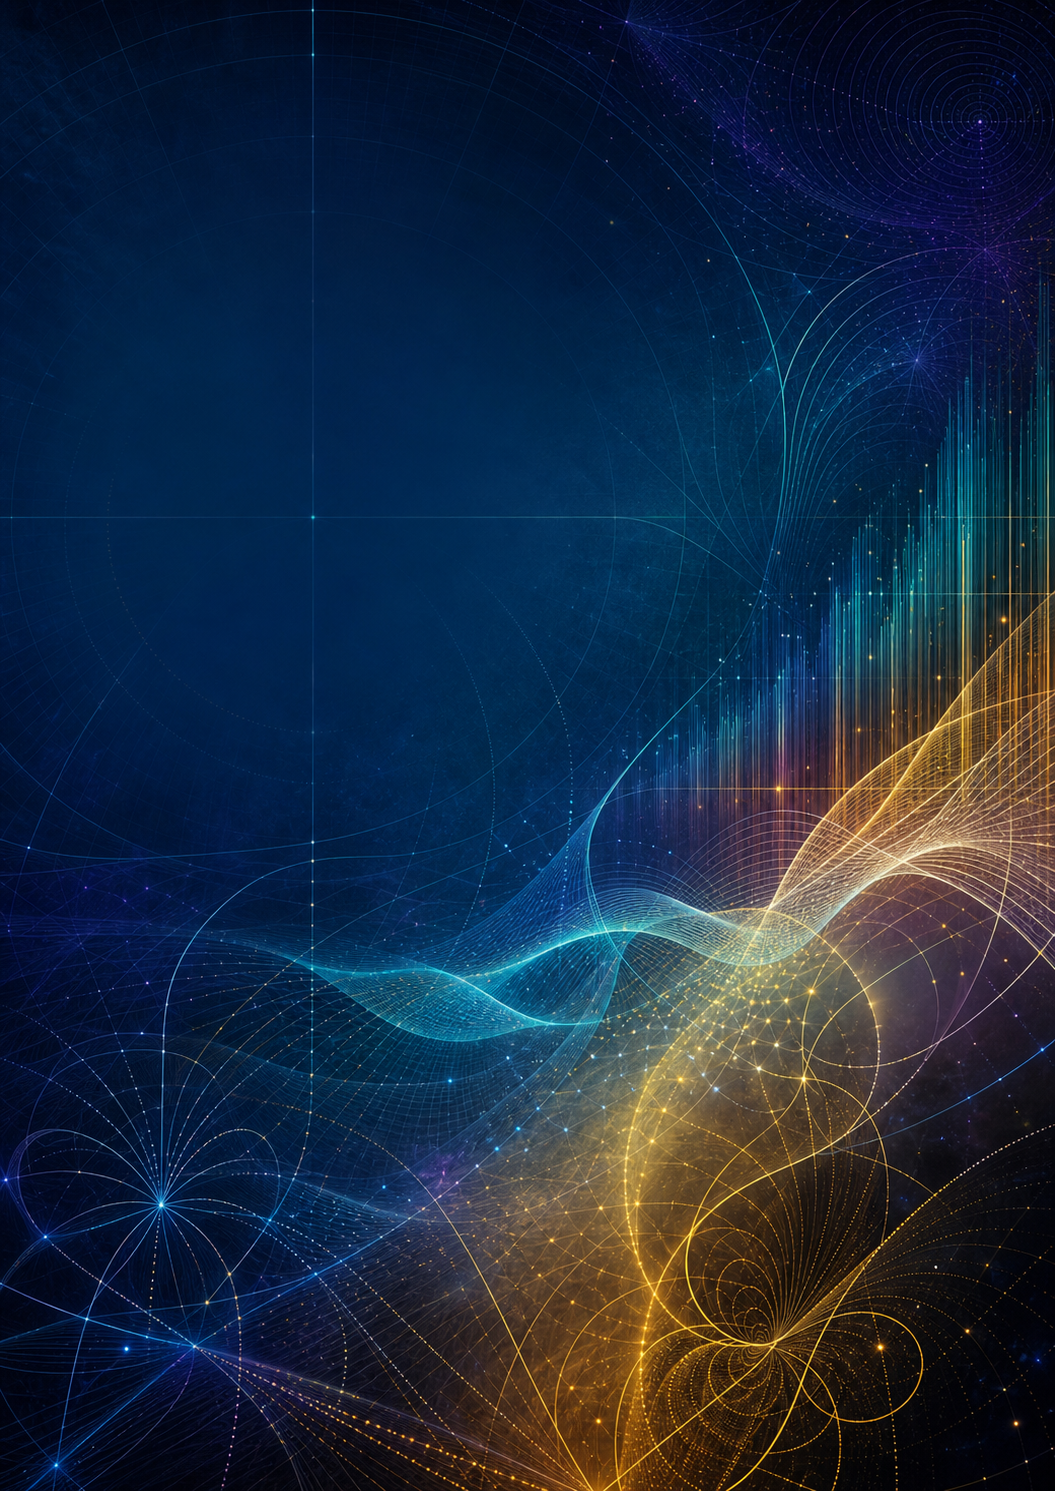
\includegraphics[width=\paperwidth,height=\paperheight]{figures/cover-image2.png}%
  };
  \fill[black, opacity=0.18] (current page.south west) rectangle (current page.north east);
  \fill[black, opacity=0.45] (current page.north west) rectangle ([yshift=-3.55in]current page.north east);
  \draw[qftCoverGold, line width=0.9pt, opacity=0.85]
    ([xshift=0.88in,yshift=-3.50in]current page.north west) --
    ([xshift=-0.88in,yshift=-3.50in]current page.north east);
  \draw[qftCoverCyan, line width=0.35pt, opacity=0.65]
    ([xshift=0.88in,yshift=-3.57in]current page.north west) --
    ([xshift=-0.88in,yshift=-3.57in]current page.north east);
\end{tikzpicture}

\vspace*{0.72in}
\begin{center}
{\sffamily\bfseries\color{white}\fontsize{32}{37}\selectfont
Quantum Field Theory\\[0.08em]from Calculus\par}

\vspace{0.34in}

{\sffamily\color{white!92}\fontsize{14}{18}\selectfont
A Self-Contained, Derivation-Based Course\\[0.12em]
from Classical Fields to Gauge Theory\par}
\end{center}
\vfill
\end{titlepage}

\clearpage
\hypersetup{pageanchor=true}
\setcounter{page}{1}
\chapter*{Preface}
\addcontentsline{toc}{chapter}{Preface}

This book is written for a reader who can differentiate, integrate, and follow an algebraic calculation, but who has not yet been handed the usual stack of prerequisites for quantum field theory.  The aim is not to hide the subject's difficulty.  The aim is to spend that difficulty carefully.

Quantum field theory is often introduced after years of linear algebra, differential equations, special relativity, quantum mechanics, and group theory.  There is a good reason for that route: each tool earns its place.  Yet the core moves of the subject are not mysterious.  They are variations of functions, sums that become integrals, oscillators that become fields, symmetries that give conserved quantities, and local changes of phase that demand gauge fields.  Each of these begins in calculus.

The chapters therefore build the machinery as it is needed.  A vector is first a list of numbers with a length.  A matrix is first a rule for mixing lists.  A delta function is first a limit of narrow peaks tested under an integral.  A path integral is first an ordinary Gaussian integral repeated many times.  A gauge field is first the price paid when a symmetry is allowed to vary from point to point.  The advanced words are not avoided, but they are made to carry their weight.

The book is not a survey.  It is a course.  Equations are derived, not merely displayed.  When a step is formal, the text says so and shows the finite-dimensional calculation that motivates it.  When an argument depends on a physical assumption, that assumption is named.  Worked examples and exercises are included so that the reader can test each new idea with a pencil rather than by nodding at prose.

No short book can replace the long apprenticeship that makes a quantum field theorist.  Still, a self-contained first road through the subject can be honest.  That is the standard used here.


\tableofcontents

\mainmatter
\part{Calculus, Space, and Mathematical Language}
\chapter{The Calculus Starting Point}

\chapterquote{A field-theory formula is useful only after the smaller calculation inside it is visible.}

This chapter is part of \emph{Calculus, Space, and Mathematical Language}.  The working vocabulary is limits, derivatives, integrals, approximation, dimensions.  The first pass through the chapter should be slow: identify the object being changed, the condition held fixed, and the reason a boundary term or normalization is allowed.  The first concrete theme is linearizing a function; later sections reuse the same habit in a more compact notation.

For The Calculus Starting Point, the calculus-level starting point is tied to linearizing a function.  Matrices, waves, operators, fields, and gauge variables are introduced only as the calculation requires them.  A formula is accepted after it has been checked in a finite model, differentiated or varied explicitly, and connected to the field-theoretic use that motivates it.

\section{The concrete problem: linearizing a function}

The work of this section is linearizing a function.  In the chapter heading the vocabulary is limits, derivatives, integrals, approximation, dimensions, but the first objects on the page are more prosaic: small changes, rates of change, accumulated area, and dimensionful quantities.  The formal notation will be useful only after it has been tied to a limit, a symmetry, a normalization condition, or an integration-by-parts step.  In The Calculus Starting Point, section 1, the useful habit is to name the object, the operation, and the assumption before using the compact notation.

The finite model is a table of sampled values \(f(x_j)\) with spacing \(\Delta x\), where derivatives are differences and integrals are sums.  In that model no mystery is available: every derivative is an ordinary derivative with respect to one listed variable, every inner product is a sum, and every boundary assumption can be written at the endpoints.  This is why the finite model is not a toy in the dismissive sense.  It is the bookkeeping device that prevents continuum notation from becoming a fog of indices.  For The Calculus Starting Point, section 1, that bookkeeping is deliberately modest, but it is what later keeps signs, factors of \(2\pi\), and normalization constants from turning into guesses.

The central idea for this chapter is linear approximation: the leading change of a quantity is the derivative multiplied by the small input change.  To test that idea, strip the formula down until only the operation remains.  A sign change after raising or lowering an index means the metric has entered.  A derivative moving from one factor to another means a boundary term has been handled.  A normalization constant means that some unit object, such as a delta function, basis vector, or one-particle state, has been fixed.  Read in the setting of The Calculus Starting Point, section 1, the line is a check on the calculation rather than an invitation to memorize another rule.

For the concrete problem: linearizing a function, the calculation should also pass a dimensional check.  The left and right sides must carry the same units; more subtly, they must transform in the same way under the symmetries already introduced.  This is not a proof, but it is a quick way to catch wrong factors of \(2\pi\), signs in the metric, missing powers of the lattice spacing, or an omitted charge.  The same step will look more abstract later; in The Calculus Starting Point, section 1 it is kept close to the finite calculation so the limiting move remains visible.

The bridge to quantum field theory is direct.  Later functional derivatives and field equations are the same idea applied to infinitely many variables labelled by position.  Later notation will carry more indices and fewer verbal reminders, so the safe habit is to keep asking which operation is being performed and which quantity is being held fixed.  At this point in The Calculus Starting Point, section 1, it is worth asking what would fail if the boundary condition, normalization, or symmetry assumption were changed.

One warning is worth making explicit here.  The symbol \(O(h^2)\) is a promise about a limit; it should not be read as a number that can be ignored at any size of \(h\).  This warning points to the delicate step of the derivation, not to a decorative aside.  In The Calculus Starting Point, section 1, the calculation is meant to leave a trail from an ordinary derivative, sum, matrix product, or Gaussian integral to the field-theory formula.

The section closes by keeping linearizing a function connected to The Calculus Starting Point.  The same general operation will be used with different objects in neighboring chapters, so the present calculation is both a result and a rehearsal.  In The Calculus Starting Point, section 1, the useful habit is to name the object, the operation, and the assumption before using the compact notation.



\paragraph{Step-by-step derivation.}

For The Calculus Starting Point: The concrete problem: linearizing a function, the derivation is written from the smallest usable model upward.

Take a differentiable function \(f\) and compare \(f(x+h)\) with \(f(x)\).  By the definition of derivative, the ratio
\[
  \frac{f(x+h)-f(x)}{h}
\]
approaches \(f'(x)\) as \(h\to0\).  Therefore the difference itself has the form
\[
  f(x+h)-f(x)=hf'(x)+h\,r(h),
\]
where \(r(h)\to0\).  If \(f\) has a second derivative, the next correction is \(\frac12h^2f''(x)\).  The expression is not a slogan about smallness; it is an accounting rule for how much information is being kept.  In The Calculus Starting Point, section 1, the useful habit is to name the object, the operation, and the assumption before using the compact notation.

The same bookkeeping explains integration by parts.  Start with the product rule \((uv)'=u'v+uv'\).  Integrating from \(a\) to \(b\) gives \(\int_a^b u'v\dd x=[uv]_a^b-\int_a^buv'\dd x\).  Every later variational derivation uses exactly this line, with \(u\) replaced by a variation or a field.  For The Calculus Starting Point, section 1, that bookkeeping is deliberately modest, but it is what later keeps signs, factors of \(2\pi\), and normalization constants from turning into guesses.

The formulas to keep in view are

\[
  f(x+h)=f(x)+hf'(x)+\frac{h^2}{2}f''(x)+O(h^3)
\]
\[
  \int_a^b u'(x)v(x)\dd x=[uv]_a^b-\int_a^b u(x)v'(x)\dd x
\]
\[
  \sum_{j=0}^{N-1}f(x_j)\Delta x\longrightarrow \int_a^b f(x)\dd x
\]

In this setting the calculation for The Calculus Starting Point: The concrete problem: linearizing a function is complete when the finite model, the limiting step, and the normalization or boundary condition can all be named without looking back at the prose.




\begin{example}[A worked calculation for The Calculus Starting Point: The concrete problem: linearizing a function]
For \(f(x)=x^2\sin(4x)\), the derivative is \(2x\sin(4x)+4x^2\cos(4x)\).  The two terms have different origins: one differentiates the slowly varying envelope, and one differentiates the oscillation.  Separating these origins is the same habit used later with fields and modes.  In The Calculus Starting Point, section 1, the useful habit is to name the object, the operation, and the assumption before using the compact notation.
\end{example}



\begin{exercise}
Differentiate \(x^2e^{-3x^2}\) and identify the two sources of terms.  Use the notation of The Calculus Starting Point: The concrete problem: linearizing a function.
\begin{answer}
\(2xe^{-3x^2}-2\cdot 3x^3e^{-3x^2}\); the two terms come from \(x^2\) and from the exponential.
\end{answer}
\end{exercise}

\begin{exercise}
State the integration-by-parts formula used in this section.  Use the notation of The Calculus Starting Point: The concrete problem: linearizing a function.
\begin{answer}
\(\int u'v=[uv]-\int uv'\), with limits or boundary conditions supplied by the problem.
\end{answer}
\end{exercise}



\section{Objects, notation, and units: tracking dimensions through a formula}

The work of this section is tracking dimensions through a formula.  In the chapter heading the vocabulary is limits, derivatives, integrals, approximation, dimensions, but the first objects on the page are more prosaic: small changes, rates of change, accumulated area, and dimensionful quantities.  The formal notation will be useful only after it has been tied to a limit, a symmetry, a normalization condition, or an integration-by-parts step.  In The Calculus Starting Point, section 2, the useful habit is to name the object, the operation, and the assumption before using the compact notation.

The finite model is a table of sampled values \(f(x_j)\) with spacing \(\Delta x\), where derivatives are differences and integrals are sums.  In that model no mystery is available: every derivative is an ordinary derivative with respect to one listed variable, every inner product is a sum, and every boundary assumption can be written at the endpoints.  This is why the finite model is not a toy in the dismissive sense.  It is the bookkeeping device that prevents continuum notation from becoming a fog of indices.  For The Calculus Starting Point, section 2, that bookkeeping is deliberately modest, but it is what later keeps signs, factors of \(2\pi\), and normalization constants from turning into guesses.

The central idea for this chapter is linear approximation: the leading change of a quantity is the derivative multiplied by the small input change.  To test that idea, strip the formula down until only the operation remains.  A sign change after raising or lowering an index means the metric has entered.  A derivative moving from one factor to another means a boundary term has been handled.  A normalization constant means that some unit object, such as a delta function, basis vector, or one-particle state, has been fixed.  Read in the setting of The Calculus Starting Point, section 2, the line is a check on the calculation rather than an invitation to memorize another rule.

For objects, notation, and units: tracking dimensions through a formula, the calculation should also pass a dimensional check.  The left and right sides must carry the same units; more subtly, they must transform in the same way under the symmetries already introduced.  This is not a proof, but it is a quick way to catch wrong factors of \(2\pi\), signs in the metric, missing powers of the lattice spacing, or an omitted charge.  The same step will look more abstract later; in The Calculus Starting Point, section 2 it is kept close to the finite calculation so the limiting move remains visible.

The bridge to quantum field theory is direct.  Later functional derivatives and field equations are the same idea applied to infinitely many variables labelled by position.  Later notation will carry more indices and fewer verbal reminders, so the safe habit is to keep asking which operation is being performed and which quantity is being held fixed.  At this point in The Calculus Starting Point, section 2, it is worth asking what would fail if the boundary condition, normalization, or symmetry assumption were changed.

One warning is worth making explicit here.  The symbol \(O(h^2)\) is a promise about a limit; it should not be read as a number that can be ignored at any size of \(h\).  This warning points to the delicate step of the derivation, not to a decorative aside.  In The Calculus Starting Point, section 2, the calculation is meant to leave a trail from an ordinary derivative, sum, matrix product, or Gaussian integral to the field-theory formula.

The section closes by keeping tracking dimensions through a formula connected to The Calculus Starting Point.  The same general operation will be used with different objects in neighboring chapters, so the present calculation is both a result and a rehearsal.  In The Calculus Starting Point, section 2, the useful habit is to name the object, the operation, and the assumption before using the compact notation.



\paragraph{Step-by-step derivation.}

For The Calculus Starting Point: Objects, notation, and units: tracking dimensions through a formula, the derivation is written from the smallest usable model upward.

Take a differentiable function \(f\) and compare \(f(x+h)\) with \(f(x)\).  By the definition of derivative, the ratio
\[
  \frac{f(x+h)-f(x)}{h}
\]
approaches \(f'(x)\) as \(h\to0\).  Therefore the difference itself has the form
\[
  f(x+h)-f(x)=hf'(x)+h\,r(h),
\]
where \(r(h)\to0\).  If \(f\) has a second derivative, the next correction is \(\frac12h^2f''(x)\).  The expression is not a slogan about smallness; it is an accounting rule for how much information is being kept.  In The Calculus Starting Point, section 2, the useful habit is to name the object, the operation, and the assumption before using the compact notation.

The same bookkeeping explains integration by parts.  Start with the product rule \((uv)'=u'v+uv'\).  Integrating from \(a\) to \(b\) gives \(\int_a^b u'v\dd x=[uv]_a^b-\int_a^buv'\dd x\).  Every later variational derivation uses exactly this line, with \(u\) replaced by a variation or a field.  For The Calculus Starting Point, section 2, that bookkeeping is deliberately modest, but it is what later keeps signs, factors of \(2\pi\), and normalization constants from turning into guesses.

The formulas to keep in view are

\[
  f(x+h)=f(x)+hf'(x)+\frac{h^2}{2}f''(x)+O(h^3)
\]
\[
  \int_a^b u'(x)v(x)\dd x=[uv]_a^b-\int_a^b u(x)v'(x)\dd x
\]
\[
  \sum_{j=0}^{N-1}f(x_j)\Delta x\longrightarrow \int_a^b f(x)\dd x
\]

In this setting the calculation for The Calculus Starting Point: Objects, notation, and units: tracking dimensions through a formula is complete when the finite model, the limiting step, and the normalization or boundary condition can all be named without looking back at the prose.




\begin{example}[A worked calculation for The Calculus Starting Point: Objects, notation, and units: tracking dimensions through a formula]
For \(f(x)=x^2\sin(5x)\), the derivative is \(2x\sin(5x)+5x^2\cos(5x)\).  The two terms have different origins: one differentiates the slowly varying envelope, and one differentiates the oscillation.  Separating these origins is the same habit used later with fields and modes.  In The Calculus Starting Point, section 2, the useful habit is to name the object, the operation, and the assumption before using the compact notation.
\end{example}



\begin{exercise}
Differentiate \(x^2e^{-4x^2}\) and identify the two sources of terms.  Use the notation of The Calculus Starting Point: Objects, notation, and units: tracking dimensions through a formula.
\begin{answer}
\(2xe^{-4x^2}-2\cdot 4x^3e^{-4x^2}\); the two terms come from \(x^2\) and from the exponential.
\end{answer}
\end{exercise}

\begin{exercise}
State the integration-by-parts formula used in this section.  Use the notation of The Calculus Starting Point: Objects, notation, and units: tracking dimensions through a formula.
\begin{answer}
\(\int u'v=[uv]-\int uv'\), with limits or boundary conditions supplied by the problem.
\end{answer}
\end{exercise}



\section{The finite calculation: turning sums into integrals}

The work of this section is turning sums into integrals.  In the chapter heading the vocabulary is limits, derivatives, integrals, approximation, dimensions, but the first objects on the page are more prosaic: small changes, rates of change, accumulated area, and dimensionful quantities.  The formal notation will be useful only after it has been tied to a limit, a symmetry, a normalization condition, or an integration-by-parts step.  In The Calculus Starting Point, section 3, the useful habit is to name the object, the operation, and the assumption before using the compact notation.

The finite model is a table of sampled values \(f(x_j)\) with spacing \(\Delta x\), where derivatives are differences and integrals are sums.  In that model no mystery is available: every derivative is an ordinary derivative with respect to one listed variable, every inner product is a sum, and every boundary assumption can be written at the endpoints.  This is why the finite model is not a toy in the dismissive sense.  It is the bookkeeping device that prevents continuum notation from becoming a fog of indices.  For The Calculus Starting Point, section 3, that bookkeeping is deliberately modest, but it is what later keeps signs, factors of \(2\pi\), and normalization constants from turning into guesses.

The central idea for this chapter is linear approximation: the leading change of a quantity is the derivative multiplied by the small input change.  To test that idea, strip the formula down until only the operation remains.  A sign change after raising or lowering an index means the metric has entered.  A derivative moving from one factor to another means a boundary term has been handled.  A normalization constant means that some unit object, such as a delta function, basis vector, or one-particle state, has been fixed.  Read in the setting of The Calculus Starting Point, section 3, the line is a check on the calculation rather than an invitation to memorize another rule.

For the finite calculation: turning sums into integrals, the calculation should also pass a dimensional check.  The left and right sides must carry the same units; more subtly, they must transform in the same way under the symmetries already introduced.  This is not a proof, but it is a quick way to catch wrong factors of \(2\pi\), signs in the metric, missing powers of the lattice spacing, or an omitted charge.  The same step will look more abstract later; in The Calculus Starting Point, section 3 it is kept close to the finite calculation so the limiting move remains visible.

The bridge to quantum field theory is direct.  Later functional derivatives and field equations are the same idea applied to infinitely many variables labelled by position.  Later notation will carry more indices and fewer verbal reminders, so the safe habit is to keep asking which operation is being performed and which quantity is being held fixed.  At this point in The Calculus Starting Point, section 3, it is worth asking what would fail if the boundary condition, normalization, or symmetry assumption were changed.

One warning is worth making explicit here.  The symbol \(O(h^2)\) is a promise about a limit; it should not be read as a number that can be ignored at any size of \(h\).  This warning points to the delicate step of the derivation, not to a decorative aside.  In The Calculus Starting Point, section 3, the calculation is meant to leave a trail from an ordinary derivative, sum, matrix product, or Gaussian integral to the field-theory formula.

The section closes by keeping turning sums into integrals connected to The Calculus Starting Point.  The same general operation will be used with different objects in neighboring chapters, so the present calculation is both a result and a rehearsal.  In The Calculus Starting Point, section 3, the useful habit is to name the object, the operation, and the assumption before using the compact notation.



\paragraph{Step-by-step derivation.}

For The Calculus Starting Point: The finite calculation: turning sums into integrals, the derivation is written from the smallest usable model upward.

Take a differentiable function \(f\) and compare \(f(x+h)\) with \(f(x)\).  By the definition of derivative, the ratio
\[
  \frac{f(x+h)-f(x)}{h}
\]
approaches \(f'(x)\) as \(h\to0\).  Therefore the difference itself has the form
\[
  f(x+h)-f(x)=hf'(x)+h\,r(h),
\]
where \(r(h)\to0\).  If \(f\) has a second derivative, the next correction is \(\frac12h^2f''(x)\).  The expression is not a slogan about smallness; it is an accounting rule for how much information is being kept.  In The Calculus Starting Point, section 3, the useful habit is to name the object, the operation, and the assumption before using the compact notation.

The same bookkeeping explains integration by parts.  Start with the product rule \((uv)'=u'v+uv'\).  Integrating from \(a\) to \(b\) gives \(\int_a^b u'v\dd x=[uv]_a^b-\int_a^buv'\dd x\).  Every later variational derivation uses exactly this line, with \(u\) replaced by a variation or a field.  For The Calculus Starting Point, section 3, that bookkeeping is deliberately modest, but it is what later keeps signs, factors of \(2\pi\), and normalization constants from turning into guesses.

The formulas to keep in view are

\[
  f(x+h)=f(x)+hf'(x)+\frac{h^2}{2}f''(x)+O(h^3)
\]
\[
  \int_a^b u'(x)v(x)\dd x=[uv]_a^b-\int_a^b u(x)v'(x)\dd x
\]
\[
  \sum_{j=0}^{N-1}f(x_j)\Delta x\longrightarrow \int_a^b f(x)\dd x
\]

In this setting the calculation for The Calculus Starting Point: The finite calculation: turning sums into integrals is complete when the finite model, the limiting step, and the normalization or boundary condition can all be named without looking back at the prose.




\begin{example}[A worked calculation for The Calculus Starting Point: The finite calculation: turning sums into integrals]
For \(f(x)=x^2\sin(6x)\), the derivative is \(2x\sin(6x)+6x^2\cos(6x)\).  The two terms have different origins: one differentiates the slowly varying envelope, and one differentiates the oscillation.  Separating these origins is the same habit used later with fields and modes.  In The Calculus Starting Point, section 3, the useful habit is to name the object, the operation, and the assumption before using the compact notation.
\end{example}



\begin{exercise}
Differentiate \(x^2e^{-5x^2}\) and identify the two sources of terms.  Use the notation of The Calculus Starting Point: The finite calculation: turning sums into integrals.
\begin{answer}
\(2xe^{-5x^2}-2\cdot 5x^3e^{-5x^2}\); the two terms come from \(x^2\) and from the exponential.
\end{answer}
\end{exercise}

\begin{exercise}
State the integration-by-parts formula used in this section.  Use the notation of The Calculus Starting Point: The finite calculation: turning sums into integrals.
\begin{answer}
\(\int u'v=[uv]-\int uv'\), with limits or boundary conditions supplied by the problem.
\end{answer}
\end{exercise}



\section{The central derivation: using integration by parts}

The work of this section is using integration by parts.  In the chapter heading the vocabulary is limits, derivatives, integrals, approximation, dimensions, but the first objects on the page are more prosaic: small changes, rates of change, accumulated area, and dimensionful quantities.  The formal notation will be useful only after it has been tied to a limit, a symmetry, a normalization condition, or an integration-by-parts step.  In The Calculus Starting Point, section 4, the useful habit is to name the object, the operation, and the assumption before using the compact notation.

The finite model is a table of sampled values \(f(x_j)\) with spacing \(\Delta x\), where derivatives are differences and integrals are sums.  In that model no mystery is available: every derivative is an ordinary derivative with respect to one listed variable, every inner product is a sum, and every boundary assumption can be written at the endpoints.  This is why the finite model is not a toy in the dismissive sense.  It is the bookkeeping device that prevents continuum notation from becoming a fog of indices.  For The Calculus Starting Point, section 4, that bookkeeping is deliberately modest, but it is what later keeps signs, factors of \(2\pi\), and normalization constants from turning into guesses.

The central idea for this chapter is linear approximation: the leading change of a quantity is the derivative multiplied by the small input change.  To test that idea, strip the formula down until only the operation remains.  A sign change after raising or lowering an index means the metric has entered.  A derivative moving from one factor to another means a boundary term has been handled.  A normalization constant means that some unit object, such as a delta function, basis vector, or one-particle state, has been fixed.  Read in the setting of The Calculus Starting Point, section 4, the line is a check on the calculation rather than an invitation to memorize another rule.

For the central derivation: using integration by parts, the calculation should also pass a dimensional check.  The left and right sides must carry the same units; more subtly, they must transform in the same way under the symmetries already introduced.  This is not a proof, but it is a quick way to catch wrong factors of \(2\pi\), signs in the metric, missing powers of the lattice spacing, or an omitted charge.  The same step will look more abstract later; in The Calculus Starting Point, section 4 it is kept close to the finite calculation so the limiting move remains visible.

The bridge to quantum field theory is direct.  Later functional derivatives and field equations are the same idea applied to infinitely many variables labelled by position.  Later notation will carry more indices and fewer verbal reminders, so the safe habit is to keep asking which operation is being performed and which quantity is being held fixed.  At this point in The Calculus Starting Point, section 4, it is worth asking what would fail if the boundary condition, normalization, or symmetry assumption were changed.

One warning is worth making explicit here.  The symbol \(O(h^2)\) is a promise about a limit; it should not be read as a number that can be ignored at any size of \(h\).  This warning points to the delicate step of the derivation, not to a decorative aside.  In The Calculus Starting Point, section 4, the calculation is meant to leave a trail from an ordinary derivative, sum, matrix product, or Gaussian integral to the field-theory formula.

The section closes by keeping using integration by parts connected to The Calculus Starting Point.  The same general operation will be used with different objects in neighboring chapters, so the present calculation is both a result and a rehearsal.  In The Calculus Starting Point, section 4, the useful habit is to name the object, the operation, and the assumption before using the compact notation.



\paragraph{Step-by-step derivation.}

For The Calculus Starting Point: The central derivation: using integration by parts, the derivation is written from the smallest usable model upward.

Take a differentiable function \(f\) and compare \(f(x+h)\) with \(f(x)\).  By the definition of derivative, the ratio
\[
  \frac{f(x+h)-f(x)}{h}
\]
approaches \(f'(x)\) as \(h\to0\).  Therefore the difference itself has the form
\[
  f(x+h)-f(x)=hf'(x)+h\,r(h),
\]
where \(r(h)\to0\).  If \(f\) has a second derivative, the next correction is \(\frac12h^2f''(x)\).  The expression is not a slogan about smallness; it is an accounting rule for how much information is being kept.  In The Calculus Starting Point, section 4, the useful habit is to name the object, the operation, and the assumption before using the compact notation.

The same bookkeeping explains integration by parts.  Start with the product rule \((uv)'=u'v+uv'\).  Integrating from \(a\) to \(b\) gives \(\int_a^b u'v\dd x=[uv]_a^b-\int_a^buv'\dd x\).  Every later variational derivation uses exactly this line, with \(u\) replaced by a variation or a field.  For The Calculus Starting Point, section 4, that bookkeeping is deliberately modest, but it is what later keeps signs, factors of \(2\pi\), and normalization constants from turning into guesses.

The formulas to keep in view are

\[
  f(x+h)=f(x)+hf'(x)+\frac{h^2}{2}f''(x)+O(h^3)
\]
\[
  \int_a^b u'(x)v(x)\dd x=[uv]_a^b-\int_a^b u(x)v'(x)\dd x
\]
\[
  \sum_{j=0}^{N-1}f(x_j)\Delta x\longrightarrow \int_a^b f(x)\dd x
\]

In this setting the calculation for The Calculus Starting Point: The central derivation: using integration by parts is complete when the finite model, the limiting step, and the normalization or boundary condition can all be named without looking back at the prose.




\begin{example}[A worked calculation for The Calculus Starting Point: The central derivation: using integration by parts]
For \(f(x)=x^2\sin(7x)\), the derivative is \(2x\sin(7x)+7x^2\cos(7x)\).  The two terms have different origins: one differentiates the slowly varying envelope, and one differentiates the oscillation.  Separating these origins is the same habit used later with fields and modes.  In The Calculus Starting Point, section 4, the useful habit is to name the object, the operation, and the assumption before using the compact notation.
\end{example}



\begin{exercise}
Differentiate \(x^2e^{-6x^2}\) and identify the two sources of terms.  Use the notation of The Calculus Starting Point: The central derivation: using integration by parts.
\begin{answer}
\(2xe^{-6x^2}-2\cdot 6x^3e^{-6x^2}\); the two terms come from \(x^2\) and from the exponential.
\end{answer}
\end{exercise}

\begin{exercise}
State the integration-by-parts formula used in this section.  Use the notation of The Calculus Starting Point: The central derivation: using integration by parts.
\begin{answer}
\(\int u'v=[uv]-\int uv'\), with limits or boundary conditions supplied by the problem.
\end{answer}
\end{exercise}



\section{Worked calculation: approximating a curve near one point}

The work of this section is approximating a curve near one point.  In the chapter heading the vocabulary is limits, derivatives, integrals, approximation, dimensions, but the first objects on the page are more prosaic: small changes, rates of change, accumulated area, and dimensionful quantities.  The formal notation will be useful only after it has been tied to a limit, a symmetry, a normalization condition, or an integration-by-parts step.  In The Calculus Starting Point, section 5, the useful habit is to name the object, the operation, and the assumption before using the compact notation.

The finite model is a table of sampled values \(f(x_j)\) with spacing \(\Delta x\), where derivatives are differences and integrals are sums.  In that model no mystery is available: every derivative is an ordinary derivative with respect to one listed variable, every inner product is a sum, and every boundary assumption can be written at the endpoints.  This is why the finite model is not a toy in the dismissive sense.  It is the bookkeeping device that prevents continuum notation from becoming a fog of indices.  For The Calculus Starting Point, section 5, that bookkeeping is deliberately modest, but it is what later keeps signs, factors of \(2\pi\), and normalization constants from turning into guesses.

The central idea for this chapter is linear approximation: the leading change of a quantity is the derivative multiplied by the small input change.  To test that idea, strip the formula down until only the operation remains.  A sign change after raising or lowering an index means the metric has entered.  A derivative moving from one factor to another means a boundary term has been handled.  A normalization constant means that some unit object, such as a delta function, basis vector, or one-particle state, has been fixed.  Read in the setting of The Calculus Starting Point, section 5, the line is a check on the calculation rather than an invitation to memorize another rule.

For worked calculation: approximating a curve near one point, the calculation should also pass a dimensional check.  The left and right sides must carry the same units; more subtly, they must transform in the same way under the symmetries already introduced.  This is not a proof, but it is a quick way to catch wrong factors of \(2\pi\), signs in the metric, missing powers of the lattice spacing, or an omitted charge.  The same step will look more abstract later; in The Calculus Starting Point, section 5 it is kept close to the finite calculation so the limiting move remains visible.

The bridge to quantum field theory is direct.  Later functional derivatives and field equations are the same idea applied to infinitely many variables labelled by position.  Later notation will carry more indices and fewer verbal reminders, so the safe habit is to keep asking which operation is being performed and which quantity is being held fixed.  At this point in The Calculus Starting Point, section 5, it is worth asking what would fail if the boundary condition, normalization, or symmetry assumption were changed.

One warning is worth making explicit here.  The symbol \(O(h^2)\) is a promise about a limit; it should not be read as a number that can be ignored at any size of \(h\).  This warning points to the delicate step of the derivation, not to a decorative aside.  In The Calculus Starting Point, section 5, the calculation is meant to leave a trail from an ordinary derivative, sum, matrix product, or Gaussian integral to the field-theory formula.

The section closes by keeping approximating a curve near one point connected to The Calculus Starting Point.  The same general operation will be used with different objects in neighboring chapters, so the present calculation is both a result and a rehearsal.  In The Calculus Starting Point, section 5, the useful habit is to name the object, the operation, and the assumption before using the compact notation.



\paragraph{Step-by-step derivation.}

For The Calculus Starting Point: Worked calculation: approximating a curve near one point, the derivation is written from the smallest usable model upward.

Take a differentiable function \(f\) and compare \(f(x+h)\) with \(f(x)\).  By the definition of derivative, the ratio
\[
  \frac{f(x+h)-f(x)}{h}
\]
approaches \(f'(x)\) as \(h\to0\).  Therefore the difference itself has the form
\[
  f(x+h)-f(x)=hf'(x)+h\,r(h),
\]
where \(r(h)\to0\).  If \(f\) has a second derivative, the next correction is \(\frac12h^2f''(x)\).  The expression is not a slogan about smallness; it is an accounting rule for how much information is being kept.  In The Calculus Starting Point, section 5, the useful habit is to name the object, the operation, and the assumption before using the compact notation.

The same bookkeeping explains integration by parts.  Start with the product rule \((uv)'=u'v+uv'\).  Integrating from \(a\) to \(b\) gives \(\int_a^b u'v\dd x=[uv]_a^b-\int_a^buv'\dd x\).  Every later variational derivation uses exactly this line, with \(u\) replaced by a variation or a field.  For The Calculus Starting Point, section 5, that bookkeeping is deliberately modest, but it is what later keeps signs, factors of \(2\pi\), and normalization constants from turning into guesses.

The formulas to keep in view are

\[
  f(x+h)=f(x)+hf'(x)+\frac{h^2}{2}f''(x)+O(h^3)
\]
\[
  \int_a^b u'(x)v(x)\dd x=[uv]_a^b-\int_a^b u(x)v'(x)\dd x
\]
\[
  \sum_{j=0}^{N-1}f(x_j)\Delta x\longrightarrow \int_a^b f(x)\dd x
\]

In this setting the calculation for The Calculus Starting Point: Worked calculation: approximating a curve near one point is complete when the finite model, the limiting step, and the normalization or boundary condition can all be named without looking back at the prose.




\begin{example}[A worked calculation for The Calculus Starting Point: Worked calculation: approximating a curve near one point]
For \(f(x)=x^2\sin(8x)\), the derivative is \(2x\sin(8x)+8x^2\cos(8x)\).  The two terms have different origins: one differentiates the slowly varying envelope, and one differentiates the oscillation.  Separating these origins is the same habit used later with fields and modes.  In The Calculus Starting Point, section 5, the useful habit is to name the object, the operation, and the assumption before using the compact notation.
\end{example}



\begin{exercise}
Differentiate \(x^2e^{-7x^2}\) and identify the two sources of terms.  Use the notation of The Calculus Starting Point: Worked calculation: approximating a curve near one point.
\begin{answer}
\(2xe^{-7x^2}-2\cdot 7x^3e^{-7x^2}\); the two terms come from \(x^2\) and from the exponential.
\end{answer}
\end{exercise}

\begin{exercise}
State the integration-by-parts formula used in this section.  Use the notation of The Calculus Starting Point: Worked calculation: approximating a curve near one point.
\begin{answer}
\(\int u'v=[uv]-\int uv'\), with limits or boundary conditions supplied by the problem.
\end{answer}
\end{exercise}



\section{Boundary conditions, normalization, and signs: controlling the error term}

The work of this section is controlling the error term.  In the chapter heading the vocabulary is limits, derivatives, integrals, approximation, dimensions, but the first objects on the page are more prosaic: small changes, rates of change, accumulated area, and dimensionful quantities.  The formal notation will be useful only after it has been tied to a limit, a symmetry, a normalization condition, or an integration-by-parts step.  In The Calculus Starting Point, section 6, the useful habit is to name the object, the operation, and the assumption before using the compact notation.

The finite model is a table of sampled values \(f(x_j)\) with spacing \(\Delta x\), where derivatives are differences and integrals are sums.  In that model no mystery is available: every derivative is an ordinary derivative with respect to one listed variable, every inner product is a sum, and every boundary assumption can be written at the endpoints.  This is why the finite model is not a toy in the dismissive sense.  It is the bookkeeping device that prevents continuum notation from becoming a fog of indices.  For The Calculus Starting Point, section 6, that bookkeeping is deliberately modest, but it is what later keeps signs, factors of \(2\pi\), and normalization constants from turning into guesses.

The central idea for this chapter is linear approximation: the leading change of a quantity is the derivative multiplied by the small input change.  To test that idea, strip the formula down until only the operation remains.  A sign change after raising or lowering an index means the metric has entered.  A derivative moving from one factor to another means a boundary term has been handled.  A normalization constant means that some unit object, such as a delta function, basis vector, or one-particle state, has been fixed.  Read in the setting of The Calculus Starting Point, section 6, the line is a check on the calculation rather than an invitation to memorize another rule.

For boundary conditions, normalization, and signs: controlling the error term, the calculation should also pass a dimensional check.  The left and right sides must carry the same units; more subtly, they must transform in the same way under the symmetries already introduced.  This is not a proof, but it is a quick way to catch wrong factors of \(2\pi\), signs in the metric, missing powers of the lattice spacing, or an omitted charge.  The same step will look more abstract later; in The Calculus Starting Point, section 6 it is kept close to the finite calculation so the limiting move remains visible.

The bridge to quantum field theory is direct.  Later functional derivatives and field equations are the same idea applied to infinitely many variables labelled by position.  Later notation will carry more indices and fewer verbal reminders, so the safe habit is to keep asking which operation is being performed and which quantity is being held fixed.  At this point in The Calculus Starting Point, section 6, it is worth asking what would fail if the boundary condition, normalization, or symmetry assumption were changed.

One warning is worth making explicit here.  The symbol \(O(h^2)\) is a promise about a limit; it should not be read as a number that can be ignored at any size of \(h\).  This warning points to the delicate step of the derivation, not to a decorative aside.  In The Calculus Starting Point, section 6, the calculation is meant to leave a trail from an ordinary derivative, sum, matrix product, or Gaussian integral to the field-theory formula.

The section closes by keeping controlling the error term connected to The Calculus Starting Point.  The same general operation will be used with different objects in neighboring chapters, so the present calculation is both a result and a rehearsal.  In The Calculus Starting Point, section 6, the useful habit is to name the object, the operation, and the assumption before using the compact notation.



\paragraph{Step-by-step derivation.}

For The Calculus Starting Point: Boundary conditions, normalization, and signs: controlling the error term, the derivation is written from the smallest usable model upward.

Take a differentiable function \(f\) and compare \(f(x+h)\) with \(f(x)\).  By the definition of derivative, the ratio
\[
  \frac{f(x+h)-f(x)}{h}
\]
approaches \(f'(x)\) as \(h\to0\).  Therefore the difference itself has the form
\[
  f(x+h)-f(x)=hf'(x)+h\,r(h),
\]
where \(r(h)\to0\).  If \(f\) has a second derivative, the next correction is \(\frac12h^2f''(x)\).  The expression is not a slogan about smallness; it is an accounting rule for how much information is being kept.  In The Calculus Starting Point, section 6, the useful habit is to name the object, the operation, and the assumption before using the compact notation.

The same bookkeeping explains integration by parts.  Start with the product rule \((uv)'=u'v+uv'\).  Integrating from \(a\) to \(b\) gives \(\int_a^b u'v\dd x=[uv]_a^b-\int_a^buv'\dd x\).  Every later variational derivation uses exactly this line, with \(u\) replaced by a variation or a field.  For The Calculus Starting Point, section 6, that bookkeeping is deliberately modest, but it is what later keeps signs, factors of \(2\pi\), and normalization constants from turning into guesses.

The formulas to keep in view are

\[
  f(x+h)=f(x)+hf'(x)+\frac{h^2}{2}f''(x)+O(h^3)
\]
\[
  \int_a^b u'(x)v(x)\dd x=[uv]_a^b-\int_a^b u(x)v'(x)\dd x
\]
\[
  \sum_{j=0}^{N-1}f(x_j)\Delta x\longrightarrow \int_a^b f(x)\dd x
\]

In this setting the calculation for The Calculus Starting Point: Boundary conditions, normalization, and signs: controlling the error term is complete when the finite model, the limiting step, and the normalization or boundary condition can all be named without looking back at the prose.




\begin{example}[A worked calculation for The Calculus Starting Point: Boundary conditions, normalization, and signs: controlling the error term]
For \(f(x)=x^2\sin(9x)\), the derivative is \(2x\sin(9x)+9x^2\cos(9x)\).  The two terms have different origins: one differentiates the slowly varying envelope, and one differentiates the oscillation.  Separating these origins is the same habit used later with fields and modes.  In The Calculus Starting Point, section 6, the useful habit is to name the object, the operation, and the assumption before using the compact notation.
\end{example}



\begin{exercise}
Differentiate \(x^2e^{-8x^2}\) and identify the two sources of terms.  Use the notation of The Calculus Starting Point: Boundary conditions, normalization, and signs: controlling the error term.
\begin{answer}
\(2xe^{-8x^2}-2\cdot 8x^3e^{-8x^2}\); the two terms come from \(x^2\) and from the exponential.
\end{answer}
\end{exercise}

\begin{exercise}
State the integration-by-parts formula used in this section.  Use the notation of The Calculus Starting Point: Boundary conditions, normalization, and signs: controlling the error term.
\begin{answer}
\(\int u'v=[uv]-\int uv'\), with limits or boundary conditions supplied by the problem.
\end{answer}
\end{exercise}



\section{How the idea enters quantum field theory: reading a differential equation locally}

The work of this section is reading a differential equation locally.  In the chapter heading the vocabulary is limits, derivatives, integrals, approximation, dimensions, but the first objects on the page are more prosaic: small changes, rates of change, accumulated area, and dimensionful quantities.  The formal notation will be useful only after it has been tied to a limit, a symmetry, a normalization condition, or an integration-by-parts step.  In The Calculus Starting Point, section 7, the useful habit is to name the object, the operation, and the assumption before using the compact notation.

The finite model is a table of sampled values \(f(x_j)\) with spacing \(\Delta x\), where derivatives are differences and integrals are sums.  In that model no mystery is available: every derivative is an ordinary derivative with respect to one listed variable, every inner product is a sum, and every boundary assumption can be written at the endpoints.  This is why the finite model is not a toy in the dismissive sense.  It is the bookkeeping device that prevents continuum notation from becoming a fog of indices.  For The Calculus Starting Point, section 7, that bookkeeping is deliberately modest, but it is what later keeps signs, factors of \(2\pi\), and normalization constants from turning into guesses.

The central idea for this chapter is linear approximation: the leading change of a quantity is the derivative multiplied by the small input change.  To test that idea, strip the formula down until only the operation remains.  A sign change after raising or lowering an index means the metric has entered.  A derivative moving from one factor to another means a boundary term has been handled.  A normalization constant means that some unit object, such as a delta function, basis vector, or one-particle state, has been fixed.  Read in the setting of The Calculus Starting Point, section 7, the line is a check on the calculation rather than an invitation to memorize another rule.

For how the idea enters quantum field theory: reading a differential equation locally, the calculation should also pass a dimensional check.  The left and right sides must carry the same units; more subtly, they must transform in the same way under the symmetries already introduced.  This is not a proof, but it is a quick way to catch wrong factors of \(2\pi\), signs in the metric, missing powers of the lattice spacing, or an omitted charge.  The same step will look more abstract later; in The Calculus Starting Point, section 7 it is kept close to the finite calculation so the limiting move remains visible.

The bridge to quantum field theory is direct.  Later functional derivatives and field equations are the same idea applied to infinitely many variables labelled by position.  Later notation will carry more indices and fewer verbal reminders, so the safe habit is to keep asking which operation is being performed and which quantity is being held fixed.  At this point in The Calculus Starting Point, section 7, it is worth asking what would fail if the boundary condition, normalization, or symmetry assumption were changed.

One warning is worth making explicit here.  The symbol \(O(h^2)\) is a promise about a limit; it should not be read as a number that can be ignored at any size of \(h\).  This warning points to the delicate step of the derivation, not to a decorative aside.  In The Calculus Starting Point, section 7, the calculation is meant to leave a trail from an ordinary derivative, sum, matrix product, or Gaussian integral to the field-theory formula.

The section closes by keeping reading a differential equation locally connected to The Calculus Starting Point.  The same general operation will be used with different objects in neighboring chapters, so the present calculation is both a result and a rehearsal.  In The Calculus Starting Point, section 7, the useful habit is to name the object, the operation, and the assumption before using the compact notation.



\paragraph{Step-by-step derivation.}

For The Calculus Starting Point: How the idea enters quantum field theory: reading a differential equation locally, the derivation is written from the smallest usable model upward.

Take a differentiable function \(f\) and compare \(f(x+h)\) with \(f(x)\).  By the definition of derivative, the ratio
\[
  \frac{f(x+h)-f(x)}{h}
\]
approaches \(f'(x)\) as \(h\to0\).  Therefore the difference itself has the form
\[
  f(x+h)-f(x)=hf'(x)+h\,r(h),
\]
where \(r(h)\to0\).  If \(f\) has a second derivative, the next correction is \(\frac12h^2f''(x)\).  The expression is not a slogan about smallness; it is an accounting rule for how much information is being kept.  In The Calculus Starting Point, section 7, the useful habit is to name the object, the operation, and the assumption before using the compact notation.

The same bookkeeping explains integration by parts.  Start with the product rule \((uv)'=u'v+uv'\).  Integrating from \(a\) to \(b\) gives \(\int_a^b u'v\dd x=[uv]_a^b-\int_a^buv'\dd x\).  Every later variational derivation uses exactly this line, with \(u\) replaced by a variation or a field.  For The Calculus Starting Point, section 7, that bookkeeping is deliberately modest, but it is what later keeps signs, factors of \(2\pi\), and normalization constants from turning into guesses.

The formulas to keep in view are

\[
  f(x+h)=f(x)+hf'(x)+\frac{h^2}{2}f''(x)+O(h^3)
\]
\[
  \int_a^b u'(x)v(x)\dd x=[uv]_a^b-\int_a^b u(x)v'(x)\dd x
\]
\[
  \sum_{j=0}^{N-1}f(x_j)\Delta x\longrightarrow \int_a^b f(x)\dd x
\]

In this setting the calculation for The Calculus Starting Point: How the idea enters quantum field theory: reading a differential equation locally is complete when the finite model, the limiting step, and the normalization or boundary condition can all be named without looking back at the prose.




\begin{example}[A worked calculation for The Calculus Starting Point: How the idea enters quantum field theory: reading a differential equation locally]
For \(f(x)=x^2\sin(10x)\), the derivative is \(2x\sin(10x)+10x^2\cos(10x)\).  The two terms have different origins: one differentiates the slowly varying envelope, and one differentiates the oscillation.  Separating these origins is the same habit used later with fields and modes.  In The Calculus Starting Point, section 7, the useful habit is to name the object, the operation, and the assumption before using the compact notation.
\end{example}



\begin{exercise}
Differentiate \(x^2e^{-9x^2}\) and identify the two sources of terms.  Use the notation of The Calculus Starting Point: How the idea enters quantum field theory: reading a differential equation locally.
\begin{answer}
\(2xe^{-9x^2}-2\cdot 9x^3e^{-9x^2}\); the two terms come from \(x^2\) and from the exponential.
\end{answer}
\end{exercise}

\begin{exercise}
State the integration-by-parts formula used in this section.  Use the notation of The Calculus Starting Point: How the idea enters quantum field theory: reading a differential equation locally.
\begin{answer}
\(\int u'v=[uv]-\int uv'\), with limits or boundary conditions supplied by the problem.
\end{answer}
\end{exercise}



\section{Review problems and extensions: building a calculation log}

The work of this section is building a calculation log.  In the chapter heading the vocabulary is limits, derivatives, integrals, approximation, dimensions, but the first objects on the page are more prosaic: small changes, rates of change, accumulated area, and dimensionful quantities.  The formal notation will be useful only after it has been tied to a limit, a symmetry, a normalization condition, or an integration-by-parts step.  In The Calculus Starting Point, section 8, the useful habit is to name the object, the operation, and the assumption before using the compact notation.

The finite model is a table of sampled values \(f(x_j)\) with spacing \(\Delta x\), where derivatives are differences and integrals are sums.  In that model no mystery is available: every derivative is an ordinary derivative with respect to one listed variable, every inner product is a sum, and every boundary assumption can be written at the endpoints.  This is why the finite model is not a toy in the dismissive sense.  It is the bookkeeping device that prevents continuum notation from becoming a fog of indices.  For The Calculus Starting Point, section 8, that bookkeeping is deliberately modest, but it is what later keeps signs, factors of \(2\pi\), and normalization constants from turning into guesses.

The central idea for this chapter is linear approximation: the leading change of a quantity is the derivative multiplied by the small input change.  To test that idea, strip the formula down until only the operation remains.  A sign change after raising or lowering an index means the metric has entered.  A derivative moving from one factor to another means a boundary term has been handled.  A normalization constant means that some unit object, such as a delta function, basis vector, or one-particle state, has been fixed.  Read in the setting of The Calculus Starting Point, section 8, the line is a check on the calculation rather than an invitation to memorize another rule.

For review problems and extensions: building a calculation log, the calculation should also pass a dimensional check.  The left and right sides must carry the same units; more subtly, they must transform in the same way under the symmetries already introduced.  This is not a proof, but it is a quick way to catch wrong factors of \(2\pi\), signs in the metric, missing powers of the lattice spacing, or an omitted charge.  The same step will look more abstract later; in The Calculus Starting Point, section 8 it is kept close to the finite calculation so the limiting move remains visible.

The bridge to quantum field theory is direct.  Later functional derivatives and field equations are the same idea applied to infinitely many variables labelled by position.  Later notation will carry more indices and fewer verbal reminders, so the safe habit is to keep asking which operation is being performed and which quantity is being held fixed.  At this point in The Calculus Starting Point, section 8, it is worth asking what would fail if the boundary condition, normalization, or symmetry assumption were changed.

One warning is worth making explicit here.  The symbol \(O(h^2)\) is a promise about a limit; it should not be read as a number that can be ignored at any size of \(h\).  This warning points to the delicate step of the derivation, not to a decorative aside.  In The Calculus Starting Point, section 8, the calculation is meant to leave a trail from an ordinary derivative, sum, matrix product, or Gaussian integral to the field-theory formula.

The section closes by keeping building a calculation log connected to The Calculus Starting Point.  The same general operation will be used with different objects in neighboring chapters, so the present calculation is both a result and a rehearsal.  In The Calculus Starting Point, section 8, the useful habit is to name the object, the operation, and the assumption before using the compact notation.



\paragraph{Step-by-step derivation.}

For The Calculus Starting Point: Review problems and extensions: building a calculation log, the derivation is written from the smallest usable model upward.

Take a differentiable function \(f\) and compare \(f(x+h)\) with \(f(x)\).  By the definition of derivative, the ratio
\[
  \frac{f(x+h)-f(x)}{h}
\]
approaches \(f'(x)\) as \(h\to0\).  Therefore the difference itself has the form
\[
  f(x+h)-f(x)=hf'(x)+h\,r(h),
\]
where \(r(h)\to0\).  If \(f\) has a second derivative, the next correction is \(\frac12h^2f''(x)\).  The expression is not a slogan about smallness; it is an accounting rule for how much information is being kept.  In The Calculus Starting Point, section 8, the useful habit is to name the object, the operation, and the assumption before using the compact notation.

The same bookkeeping explains integration by parts.  Start with the product rule \((uv)'=u'v+uv'\).  Integrating from \(a\) to \(b\) gives \(\int_a^b u'v\dd x=[uv]_a^b-\int_a^buv'\dd x\).  Every later variational derivation uses exactly this line, with \(u\) replaced by a variation or a field.  For The Calculus Starting Point, section 8, that bookkeeping is deliberately modest, but it is what later keeps signs, factors of \(2\pi\), and normalization constants from turning into guesses.

The formulas to keep in view are

\[
  f(x+h)=f(x)+hf'(x)+\frac{h^2}{2}f''(x)+O(h^3)
\]
\[
  \int_a^b u'(x)v(x)\dd x=[uv]_a^b-\int_a^b u(x)v'(x)\dd x
\]
\[
  \sum_{j=0}^{N-1}f(x_j)\Delta x\longrightarrow \int_a^b f(x)\dd x
\]

In this setting the calculation for The Calculus Starting Point: Review problems and extensions: building a calculation log is complete when the finite model, the limiting step, and the normalization or boundary condition can all be named without looking back at the prose.




\begin{example}[A worked calculation for The Calculus Starting Point: Review problems and extensions: building a calculation log]
For \(f(x)=x^2\sin(11x)\), the derivative is \(2x\sin(11x)+11x^2\cos(11x)\).  The two terms have different origins: one differentiates the slowly varying envelope, and one differentiates the oscillation.  Separating these origins is the same habit used later with fields and modes.  In The Calculus Starting Point, section 8, the useful habit is to name the object, the operation, and the assumption before using the compact notation.
\end{example}



\begin{exercise}
Differentiate \(x^2e^{-10x^2}\) and identify the two sources of terms.  Use the notation of The Calculus Starting Point: Review problems and extensions: building a calculation log.
\begin{answer}
\(2xe^{-10x^2}-2\cdot 10x^3e^{-10x^2}\); the two terms come from \(x^2\) and from the exponential.
\end{answer}
\end{exercise}

\begin{exercise}
State the integration-by-parts formula used in this section.  Use the notation of The Calculus Starting Point: Review problems and extensions: building a calculation log.
\begin{answer}
\(\int u'v=[uv]-\int uv'\), with limits or boundary conditions supplied by the problem.
\end{answer}
\end{exercise}



\section{Cumulative worked derivation: from linearizing a function to reading a differential equation locally}

This final worked section braids together linearizing a function, using integration by parts, and reading a differential equation locally for The Calculus Starting Point.  The vocabulary of the chapter was limits, derivatives, integrals, approximation, dimensions; here those words are used in one continuous calculation rather than in isolated fragments.

Choose a small change, compute the linear term, check units, and then ask whether the same operation survives a limiting process.  This is the common skeleton behind derivatives, matrix actions, Fourier transforms, and field variations.  The notation grows, but the controlling questions remain the same: what is varied, what is fixed, which boundary term is used, and what finite calculation is being approximated?  In The Calculus Starting Point, cumulative derivation, the useful habit is to name the object, the operation, and the assumption before using the compact notation.

For reference, the compact formulas are

\[
  f(x+h)=f(x)+hf'(x)+\frac{h^2}{2}f''(x)+O(h^3)
\]
\[
  \int_a^b u'(x)v(x)\dd x=[uv]_a^b-\int_a^b u(x)v'(x)\dd x
\]
\[
  \sum_{j=0}^{N-1}f(x_j)\Delta x\longrightarrow \int_a^b f(x)\dd x
\]

\begin{exercise}
Reproduce the cumulative derivation for The Calculus Starting Point without looking at the prose.  Mark the step where a finite calculation becomes a continuum, operator, or field-theoretic statement.
\begin{answer}
The reconstruction should name the starting object, carry out the differentiating, varying, transforming, or commuting step explicitly, and state the normalization or boundary condition that makes the final formula meaningful.
\end{answer}
\end{exercise}



\section{Chapter synthesis}

This chapter has treated the calculus starting point as a chain of calculations.  The safest summary is not a list of final formulas, but a map from assumptions to equations: finite model, limiting step, boundary condition, normalization, and field-theory use.  If one of those links is missing, the formula should be rederived before it is used in a later chapter.

\begin{exercise}
Write a one-page reconstruction of the calculus starting point.  Include one equation from the finite model, one equation from the continuum or operator form, and one sentence explaining how the two are connected.
\begin{answer}
A strong reconstruction names the basic objects, identifies the central derivative, variation, commutator, or symmetry operation, and states the assumption that allows the finite calculation to become the field-theory formula.
\end{answer}
\end{exercise}

\chapter{Vectors, Coordinates, and Geometry}

\chapterquote{A field-theory formula is useful only after the smaller calculation inside it is visible.}

This chapter is part of \emph{Calculus, Space, and Mathematical Language}.  The working vocabulary is vectors, coordinates, dot products, bases, length.  The first pass through the chapter should be slow: identify the object being changed, the condition held fixed, and the reason a boundary term or normalization is allowed.  The first concrete theme is separating vectors from coordinates; later sections reuse the same habit in a more compact notation.

For Vectors, Coordinates, and Geometry, the calculus-level starting point is tied to separating vectors from coordinates.  Matrices, waves, operators, fields, and gauge variables are introduced only as the calculation requires them.  A formula is accepted after it has been checked in a finite model, differentiated or varied explicitly, and connected to the field-theoretic use that motivates it.

\section{The concrete problem: separating vectors from coordinates}

% QFTFIGURE-BEGIN ch002vectorscoordinatesandgeometry-01-vector-arrow
\qftfigure{figures/instructional/ch002vectorscoordinatesandgeometry/ch002vectorscoordinatesandgeometry-01-vector-arrow.pdf}{The fixed arrow with two coordinate grids separates the geometric object from the component lists used to describe it.}{fig:ch002vectorscoordinatesandgeometry-01-vector-arrow}
% QFTFIGURE-END ch002vectorscoordinatesandgeometry-01-vector-arrow












The work of this section is separating vectors from coordinates.  In the chapter heading the vocabulary is vectors, coordinates, dot products, bases, length, but the first objects on the page are more prosaic: arrows, coordinates, basis vectors, dot products, lengths, and projections.  The formal notation will be useful only after it has been tied to a limit, a symmetry, a normalization condition, or an integration-by-parts step.  In Vectors, Coordinates, and Geometry, section 1, the useful habit is to name the object, the operation, and the assumption before using the compact notation.

The finite model is a two- or three-component column vector whose components change when the basis is changed.  In that model no mystery is available: every derivative is an ordinary derivative with respect to one listed variable, every inner product is a sum, and every boundary assumption can be written at the endpoints.  This is why the finite model is not a toy in the dismissive sense.  It is the bookkeeping device that prevents continuum notation from becoming a fog of indices.  For Vectors, Coordinates, and Geometry, section 1, that bookkeeping is deliberately modest, but it is what later keeps signs, factors of \(2\pi\), and normalization constants from turning into guesses.

The central idea for this chapter is a geometric statement must keep the same length and angle even when coordinates are rewritten.  To test that idea, strip the formula down until only the operation remains.  A sign change after raising or lowering an index means the metric has entered.  A derivative moving from one factor to another means a boundary term has been handled.  A normalization constant means that some unit object, such as a delta function, basis vector, or one-particle state, has been fixed.  Read in the setting of Vectors, Coordinates, and Geometry, section 1, the line is a check on the calculation rather than an invitation to memorize another rule.

For the concrete problem: separating vectors from coordinates, the calculation should also pass a dimensional check.  The left and right sides must carry the same units; more subtly, they must transform in the same way under the symmetries already introduced.  This is not a proof, but it is a quick way to catch wrong factors of \(2\pi\), signs in the metric, missing powers of the lattice spacing, or an omitted charge.  The same step will look more abstract later; in Vectors, Coordinates, and Geometry, section 1 it is kept close to the finite calculation so the limiting move remains visible.

The bridge to quantum field theory is direct.  Fields will later have components under rotations, Lorentz transformations, and internal symmetry rotations.  Later notation will carry more indices and fewer verbal reminders, so the safe habit is to keep asking which operation is being performed and which quantity is being held fixed.  At this point in Vectors, Coordinates, and Geometry, section 1, it is worth asking what would fail if the boundary condition, normalization, or symmetry assumption were changed.

One warning is worth making explicit here.  A component is not the vector itself; changing coordinates changes the component list without changing the arrow.  This warning points to the delicate step of the derivation, not to a decorative aside.  In Vectors, Coordinates, and Geometry, section 1, the calculation is meant to leave a trail from an ordinary derivative, sum, matrix product, or Gaussian integral to the field-theory formula.

The section closes by keeping separating vectors from coordinates connected to Vectors, Coordinates, and Geometry.  The same general operation will be used with different objects in neighboring chapters, so the present calculation is both a result and a rehearsal.  In Vectors, Coordinates, and Geometry, section 1, the useful habit is to name the object, the operation, and the assumption before using the compact notation.



\paragraph{Step-by-step derivation.}

For Vectors, Coordinates, and Geometry: The concrete problem: separating vectors from coordinates, the derivation is written from the smallest usable model upward.

Let \(\hat n\) be a unit vector.  The component of \(\bm v\) along \(\hat n\) is the number \(c\) for which \(c\hat n\) is the closest vector on the line spanned by \(\hat n\).  Minimize \(\|\bm v-c\hat n\|^2\):
\[
  \|\bm v-c\hat n\|^2=\bm v\cdot\bm v-2c\,\bm v\cdot\hat n+c^2.
\]
Differentiating with respect to \(c\) gives \(-2\bm v\cdot\hat n+2c=0\), hence \(c=\bm v\cdot\hat n\).  Thus projection is not a memorized formula; it is a one-variable minimization problem.  In Vectors, Coordinates, and Geometry, section 1, the useful habit is to name the object, the operation, and the assumption before using the compact notation.

When the basis changes, the arrow has not changed.  If \(\bm v=v^i\bm e_i=\tilde v^i\tilde{\bm e}_i\), the component lists differ because the basis vectors differ.  This distinction is the seed of tensor notation.  For Vectors, Coordinates, and Geometry, section 1, that bookkeeping is deliberately modest, but it is what later keeps signs, factors of \(2\pi\), and normalization constants from turning into guesses.

The formulas to keep in view are

\[
  \bm v=v^i\bm e_i,\qquad \bm v\cdot\bm w=v^iw^j(\bm e_i\cdot\bm e_j)
\]
\[
  \mathrm{proj}_{\hat n}\bm v=(\bm v\cdot\hat n)\hat n
\]
\[
  A\bm e_j=A^i{}_j\bm e_i
\]

In this setting the calculation for Vectors, Coordinates, and Geometry: The concrete problem: separating vectors from coordinates is complete when the finite model, the limiting step, and the normalization or boundary condition can all be named without looking back at the prose.




\begin{example}[A worked calculation for Vectors, Coordinates, and Geometry: The concrete problem: separating vectors from coordinates]
Take \(\bm v=(3,4)\) and \(\hat n=(1,0)\) in an orthonormal basis.  The projection coefficient is
\[
  \bm v\cdot\hat n=3,
\]
so the projected vector is \((3,0)\).  If the basis is rotated, the component list changes, but the length of the projected vector remains \(3\).  This is the small finite-dimensional check behind later statements about tensors and invariant inner products.  In Vectors, Coordinates, and Geometry, section 1, the useful habit is to name the object, the operation, and the assumption before using the compact notation.
\end{example}



\begin{exercise}
For \(\bm v=(2,-1,2)\), compute its length in an orthonormal basis.  Use the notation of Vectors, Coordinates, and Geometry: The concrete problem: separating vectors from coordinates.
\begin{answer}
The length is \(\sqrt{2^2+(-1)^2+2^2}=3\).
\end{answer}
\end{exercise}

\begin{exercise}
Let \(\hat n=(0,1)\) and \(\bm v=(5,-2)\).  Compute the projection of \(\bm v\) onto \(\hat n\).  Use the notation of Vectors, Coordinates, and Geometry: The concrete problem: separating vectors from coordinates.
\begin{answer}
The coefficient is \(\bm v\cdot\hat n=-2\), so the projected vector is \((0,-2)\).
\end{answer}
\end{exercise}



\section{Objects, notation, and units: computing projections}

% QFTFIGURE-BEGIN ch002vectorscoordinatesandgeometry-02-projection
\qftfigure{figures/instructional/ch002vectorscoordinatesandgeometry/ch002vectorscoordinatesandgeometry-02-projection.pdf}{The right-triangle projection makes the dot product visible as the amount of one direction contained in another.}{fig:ch002vectorscoordinatesandgeometry-02-projection}
% QFTFIGURE-END ch002vectorscoordinatesandgeometry-02-projection












The work of this section is computing projections.  In the chapter heading the vocabulary is vectors, coordinates, dot products, bases, length, but the first objects on the page are more prosaic: arrows, coordinates, basis vectors, dot products, lengths, and projections.  The formal notation will be useful only after it has been tied to a limit, a symmetry, a normalization condition, or an integration-by-parts step.  In Vectors, Coordinates, and Geometry, section 2, the useful habit is to name the object, the operation, and the assumption before using the compact notation.

The finite model is a two- or three-component column vector whose components change when the basis is changed.  In that model no mystery is available: every derivative is an ordinary derivative with respect to one listed variable, every inner product is a sum, and every boundary assumption can be written at the endpoints.  This is why the finite model is not a toy in the dismissive sense.  It is the bookkeeping device that prevents continuum notation from becoming a fog of indices.  For Vectors, Coordinates, and Geometry, section 2, that bookkeeping is deliberately modest, but it is what later keeps signs, factors of \(2\pi\), and normalization constants from turning into guesses.

The central idea for this chapter is a geometric statement must keep the same length and angle even when coordinates are rewritten.  To test that idea, strip the formula down until only the operation remains.  A sign change after raising or lowering an index means the metric has entered.  A derivative moving from one factor to another means a boundary term has been handled.  A normalization constant means that some unit object, such as a delta function, basis vector, or one-particle state, has been fixed.  Read in the setting of Vectors, Coordinates, and Geometry, section 2, the line is a check on the calculation rather than an invitation to memorize another rule.

For objects, notation, and units: computing projections, the calculation should also pass a dimensional check.  The left and right sides must carry the same units; more subtly, they must transform in the same way under the symmetries already introduced.  This is not a proof, but it is a quick way to catch wrong factors of \(2\pi\), signs in the metric, missing powers of the lattice spacing, or an omitted charge.  The same step will look more abstract later; in Vectors, Coordinates, and Geometry, section 2 it is kept close to the finite calculation so the limiting move remains visible.

The bridge to quantum field theory is direct.  Fields will later have components under rotations, Lorentz transformations, and internal symmetry rotations.  Later notation will carry more indices and fewer verbal reminders, so the safe habit is to keep asking which operation is being performed and which quantity is being held fixed.  At this point in Vectors, Coordinates, and Geometry, section 2, it is worth asking what would fail if the boundary condition, normalization, or symmetry assumption were changed.

One warning is worth making explicit here.  A component is not the vector itself; changing coordinates changes the component list without changing the arrow.  This warning points to the delicate step of the derivation, not to a decorative aside.  In Vectors, Coordinates, and Geometry, section 2, the calculation is meant to leave a trail from an ordinary derivative, sum, matrix product, or Gaussian integral to the field-theory formula.

The section closes by keeping computing projections connected to Vectors, Coordinates, and Geometry.  The same general operation will be used with different objects in neighboring chapters, so the present calculation is both a result and a rehearsal.  In Vectors, Coordinates, and Geometry, section 2, the useful habit is to name the object, the operation, and the assumption before using the compact notation.



\paragraph{Step-by-step derivation.}

For Vectors, Coordinates, and Geometry: Objects, notation, and units: computing projections, the derivation is written from the smallest usable model upward.

Let \(\hat n\) be a unit vector.  The component of \(\bm v\) along \(\hat n\) is the number \(c\) for which \(c\hat n\) is the closest vector on the line spanned by \(\hat n\).  Minimize \(\|\bm v-c\hat n\|^2\):
\[
  \|\bm v-c\hat n\|^2=\bm v\cdot\bm v-2c\,\bm v\cdot\hat n+c^2.
\]
Differentiating with respect to \(c\) gives \(-2\bm v\cdot\hat n+2c=0\), hence \(c=\bm v\cdot\hat n\).  Thus projection is not a memorized formula; it is a one-variable minimization problem.  In Vectors, Coordinates, and Geometry, section 2, the useful habit is to name the object, the operation, and the assumption before using the compact notation.

When the basis changes, the arrow has not changed.  If \(\bm v=v^i\bm e_i=\tilde v^i\tilde{\bm e}_i\), the component lists differ because the basis vectors differ.  This distinction is the seed of tensor notation.  For Vectors, Coordinates, and Geometry, section 2, that bookkeeping is deliberately modest, but it is what later keeps signs, factors of \(2\pi\), and normalization constants from turning into guesses.

The formulas to keep in view are

\[
  \bm v=v^i\bm e_i,\qquad \bm v\cdot\bm w=v^iw^j(\bm e_i\cdot\bm e_j)
\]
\[
  \mathrm{proj}_{\hat n}\bm v=(\bm v\cdot\hat n)\hat n
\]
\[
  A\bm e_j=A^i{}_j\bm e_i
\]

In this setting the calculation for Vectors, Coordinates, and Geometry: Objects, notation, and units: computing projections is complete when the finite model, the limiting step, and the normalization or boundary condition can all be named without looking back at the prose.




\begin{example}[A worked calculation for Vectors, Coordinates, and Geometry: Objects, notation, and units: computing projections]
Take \(\bm v=(3,4)\) and \(\hat n=(1,0)\) in an orthonormal basis.  The projection coefficient is
\[
  \bm v\cdot\hat n=3,
\]
so the projected vector is \((3,0)\).  If the basis is rotated, the component list changes, but the length of the projected vector remains \(3\).  This is the small finite-dimensional check behind later statements about tensors and invariant inner products.  In Vectors, Coordinates, and Geometry, section 2, the useful habit is to name the object, the operation, and the assumption before using the compact notation.
\end{example}



\begin{exercise}
For \(\bm v=(2,-1,2)\), compute its length in an orthonormal basis.  Use the notation of Vectors, Coordinates, and Geometry: Objects, notation, and units: computing projections.
\begin{answer}
The length is \(\sqrt{2^2+(-1)^2+2^2}=3\).
\end{answer}
\end{exercise}

\begin{exercise}
Let \(\hat n=(0,1)\) and \(\bm v=(5,-2)\).  Compute the projection of \(\bm v\) onto \(\hat n\).  Use the notation of Vectors, Coordinates, and Geometry: Objects, notation, and units: computing projections.
\begin{answer}
The coefficient is \(\bm v\cdot\hat n=-2\), so the projected vector is \((0,-2)\).
\end{answer}
\end{exercise}



\section{The finite calculation: changing bases}

% QFTFIGURE-BEGIN ch002vectorscoordinatesandgeometry-03-basis-change
\qftfigure{figures/instructional/ch002vectorscoordinatesandgeometry/ch002vectorscoordinatesandgeometry-03-basis-change.pdf}{The rotated grids show that components can change while the vector and its physical length remain unchanged.}{fig:ch002vectorscoordinatesandgeometry-03-basis-change}
% QFTFIGURE-END ch002vectorscoordinatesandgeometry-03-basis-change












The work of this section is changing bases.  In the chapter heading the vocabulary is vectors, coordinates, dot products, bases, length, but the first objects on the page are more prosaic: arrows, coordinates, basis vectors, dot products, lengths, and projections.  The formal notation will be useful only after it has been tied to a limit, a symmetry, a normalization condition, or an integration-by-parts step.  In Vectors, Coordinates, and Geometry, section 3, the useful habit is to name the object, the operation, and the assumption before using the compact notation.

The finite model is a two- or three-component column vector whose components change when the basis is changed.  In that model no mystery is available: every derivative is an ordinary derivative with respect to one listed variable, every inner product is a sum, and every boundary assumption can be written at the endpoints.  This is why the finite model is not a toy in the dismissive sense.  It is the bookkeeping device that prevents continuum notation from becoming a fog of indices.  For Vectors, Coordinates, and Geometry, section 3, that bookkeeping is deliberately modest, but it is what later keeps signs, factors of \(2\pi\), and normalization constants from turning into guesses.

The central idea for this chapter is a geometric statement must keep the same length and angle even when coordinates are rewritten.  To test that idea, strip the formula down until only the operation remains.  A sign change after raising or lowering an index means the metric has entered.  A derivative moving from one factor to another means a boundary term has been handled.  A normalization constant means that some unit object, such as a delta function, basis vector, or one-particle state, has been fixed.  Read in the setting of Vectors, Coordinates, and Geometry, section 3, the line is a check on the calculation rather than an invitation to memorize another rule.

For the finite calculation: changing bases, the calculation should also pass a dimensional check.  The left and right sides must carry the same units; more subtly, they must transform in the same way under the symmetries already introduced.  This is not a proof, but it is a quick way to catch wrong factors of \(2\pi\), signs in the metric, missing powers of the lattice spacing, or an omitted charge.  The same step will look more abstract later; in Vectors, Coordinates, and Geometry, section 3 it is kept close to the finite calculation so the limiting move remains visible.

The bridge to quantum field theory is direct.  Fields will later have components under rotations, Lorentz transformations, and internal symmetry rotations.  Later notation will carry more indices and fewer verbal reminders, so the safe habit is to keep asking which operation is being performed and which quantity is being held fixed.  At this point in Vectors, Coordinates, and Geometry, section 3, it is worth asking what would fail if the boundary condition, normalization, or symmetry assumption were changed.

One warning is worth making explicit here.  A component is not the vector itself; changing coordinates changes the component list without changing the arrow.  This warning points to the delicate step of the derivation, not to a decorative aside.  In Vectors, Coordinates, and Geometry, section 3, the calculation is meant to leave a trail from an ordinary derivative, sum, matrix product, or Gaussian integral to the field-theory formula.

The section closes by keeping changing bases connected to Vectors, Coordinates, and Geometry.  The same general operation will be used with different objects in neighboring chapters, so the present calculation is both a result and a rehearsal.  In Vectors, Coordinates, and Geometry, section 3, the useful habit is to name the object, the operation, and the assumption before using the compact notation.



\paragraph{Step-by-step derivation.}

For Vectors, Coordinates, and Geometry: The finite calculation: changing bases, the derivation is written from the smallest usable model upward.

Let \(\hat n\) be a unit vector.  The component of \(\bm v\) along \(\hat n\) is the number \(c\) for which \(c\hat n\) is the closest vector on the line spanned by \(\hat n\).  Minimize \(\|\bm v-c\hat n\|^2\):
\[
  \|\bm v-c\hat n\|^2=\bm v\cdot\bm v-2c\,\bm v\cdot\hat n+c^2.
\]
Differentiating with respect to \(c\) gives \(-2\bm v\cdot\hat n+2c=0\), hence \(c=\bm v\cdot\hat n\).  Thus projection is not a memorized formula; it is a one-variable minimization problem.  In Vectors, Coordinates, and Geometry, section 3, the useful habit is to name the object, the operation, and the assumption before using the compact notation.

When the basis changes, the arrow has not changed.  If \(\bm v=v^i\bm e_i=\tilde v^i\tilde{\bm e}_i\), the component lists differ because the basis vectors differ.  This distinction is the seed of tensor notation.  For Vectors, Coordinates, and Geometry, section 3, that bookkeeping is deliberately modest, but it is what later keeps signs, factors of \(2\pi\), and normalization constants from turning into guesses.

The formulas to keep in view are

\[
  \bm v=v^i\bm e_i,\qquad \bm v\cdot\bm w=v^iw^j(\bm e_i\cdot\bm e_j)
\]
\[
  \mathrm{proj}_{\hat n}\bm v=(\bm v\cdot\hat n)\hat n
\]
\[
  A\bm e_j=A^i{}_j\bm e_i
\]

In this setting the calculation for Vectors, Coordinates, and Geometry: The finite calculation: changing bases is complete when the finite model, the limiting step, and the normalization or boundary condition can all be named without looking back at the prose.




\begin{example}[A worked calculation for Vectors, Coordinates, and Geometry: The finite calculation: changing bases]
Take \(\bm v=(3,4)\) and \(\hat n=(1,0)\) in an orthonormal basis.  The projection coefficient is
\[
  \bm v\cdot\hat n=3,
\]
so the projected vector is \((3,0)\).  If the basis is rotated, the component list changes, but the length of the projected vector remains \(3\).  This is the small finite-dimensional check behind later statements about tensors and invariant inner products.  In Vectors, Coordinates, and Geometry, section 3, the useful habit is to name the object, the operation, and the assumption before using the compact notation.
\end{example}



\begin{exercise}
For \(\bm v=(2,-1,2)\), compute its length in an orthonormal basis.  Use the notation of Vectors, Coordinates, and Geometry: The finite calculation: changing bases.
\begin{answer}
The length is \(\sqrt{2^2+(-1)^2+2^2}=3\).
\end{answer}
\end{exercise}

\begin{exercise}
Let \(\hat n=(0,1)\) and \(\bm v=(5,-2)\).  Compute the projection of \(\bm v\) onto \(\hat n\).  Use the notation of Vectors, Coordinates, and Geometry: The finite calculation: changing bases.
\begin{answer}
The coefficient is \(\bm v\cdot\hat n=-2\), so the projected vector is \((0,-2)\).
\end{answer}
\end{exercise}



\section{The central derivation: dot products as measurements}

% QFTFIGURE-BEGIN ch002vectorscoordinatesandgeometry-04-metric-length
\qftfigure{figures/instructional/ch002vectorscoordinatesandgeometry/ch002vectorscoordinatesandgeometry-04-metric-length.pdf}{The ellipse of equal length illustrates how a metric turns coordinate differences into invariant geometric measurements.}{fig:ch002vectorscoordinatesandgeometry-04-metric-length}
% QFTFIGURE-END ch002vectorscoordinatesandgeometry-04-metric-length












The work of this section is dot products as measurements.  In the chapter heading the vocabulary is vectors, coordinates, dot products, bases, length, but the first objects on the page are more prosaic: arrows, coordinates, basis vectors, dot products, lengths, and projections.  The formal notation will be useful only after it has been tied to a limit, a symmetry, a normalization condition, or an integration-by-parts step.  In Vectors, Coordinates, and Geometry, section 4, the useful habit is to name the object, the operation, and the assumption before using the compact notation.

The finite model is a two- or three-component column vector whose components change when the basis is changed.  In that model no mystery is available: every derivative is an ordinary derivative with respect to one listed variable, every inner product is a sum, and every boundary assumption can be written at the endpoints.  This is why the finite model is not a toy in the dismissive sense.  It is the bookkeeping device that prevents continuum notation from becoming a fog of indices.  For Vectors, Coordinates, and Geometry, section 4, that bookkeeping is deliberately modest, but it is what later keeps signs, factors of \(2\pi\), and normalization constants from turning into guesses.

The central idea for this chapter is a geometric statement must keep the same length and angle even when coordinates are rewritten.  To test that idea, strip the formula down until only the operation remains.  A sign change after raising or lowering an index means the metric has entered.  A derivative moving from one factor to another means a boundary term has been handled.  A normalization constant means that some unit object, such as a delta function, basis vector, or one-particle state, has been fixed.  Read in the setting of Vectors, Coordinates, and Geometry, section 4, the line is a check on the calculation rather than an invitation to memorize another rule.

For the central derivation: dot products as measurements, the calculation should also pass a dimensional check.  The left and right sides must carry the same units; more subtly, they must transform in the same way under the symmetries already introduced.  This is not a proof, but it is a quick way to catch wrong factors of \(2\pi\), signs in the metric, missing powers of the lattice spacing, or an omitted charge.  The same step will look more abstract later; in Vectors, Coordinates, and Geometry, section 4 it is kept close to the finite calculation so the limiting move remains visible.

The bridge to quantum field theory is direct.  Fields will later have components under rotations, Lorentz transformations, and internal symmetry rotations.  Later notation will carry more indices and fewer verbal reminders, so the safe habit is to keep asking which operation is being performed and which quantity is being held fixed.  At this point in Vectors, Coordinates, and Geometry, section 4, it is worth asking what would fail if the boundary condition, normalization, or symmetry assumption were changed.

One warning is worth making explicit here.  A component is not the vector itself; changing coordinates changes the component list without changing the arrow.  This warning points to the delicate step of the derivation, not to a decorative aside.  In Vectors, Coordinates, and Geometry, section 4, the calculation is meant to leave a trail from an ordinary derivative, sum, matrix product, or Gaussian integral to the field-theory formula.

The section closes by keeping dot products as measurements connected to Vectors, Coordinates, and Geometry.  The same general operation will be used with different objects in neighboring chapters, so the present calculation is both a result and a rehearsal.  In Vectors, Coordinates, and Geometry, section 4, the useful habit is to name the object, the operation, and the assumption before using the compact notation.



\paragraph{Step-by-step derivation.}

For Vectors, Coordinates, and Geometry: The central derivation: dot products as measurements, the derivation is written from the smallest usable model upward.

Let \(\hat n\) be a unit vector.  The component of \(\bm v\) along \(\hat n\) is the number \(c\) for which \(c\hat n\) is the closest vector on the line spanned by \(\hat n\).  Minimize \(\|\bm v-c\hat n\|^2\):
\[
  \|\bm v-c\hat n\|^2=\bm v\cdot\bm v-2c\,\bm v\cdot\hat n+c^2.
\]
Differentiating with respect to \(c\) gives \(-2\bm v\cdot\hat n+2c=0\), hence \(c=\bm v\cdot\hat n\).  Thus projection is not a memorized formula; it is a one-variable minimization problem.  In Vectors, Coordinates, and Geometry, section 4, the useful habit is to name the object, the operation, and the assumption before using the compact notation.

When the basis changes, the arrow has not changed.  If \(\bm v=v^i\bm e_i=\tilde v^i\tilde{\bm e}_i\), the component lists differ because the basis vectors differ.  This distinction is the seed of tensor notation.  For Vectors, Coordinates, and Geometry, section 4, that bookkeeping is deliberately modest, but it is what later keeps signs, factors of \(2\pi\), and normalization constants from turning into guesses.

The formulas to keep in view are

\[
  \bm v=v^i\bm e_i,\qquad \bm v\cdot\bm w=v^iw^j(\bm e_i\cdot\bm e_j)
\]
\[
  \mathrm{proj}_{\hat n}\bm v=(\bm v\cdot\hat n)\hat n
\]
\[
  A\bm e_j=A^i{}_j\bm e_i
\]

In this setting the calculation for Vectors, Coordinates, and Geometry: The central derivation: dot products as measurements is complete when the finite model, the limiting step, and the normalization or boundary condition can all be named without looking back at the prose.




\begin{example}[A worked calculation for Vectors, Coordinates, and Geometry: The central derivation: dot products as measurements]
Take \(\bm v=(3,4)\) and \(\hat n=(1,0)\) in an orthonormal basis.  The projection coefficient is
\[
  \bm v\cdot\hat n=3,
\]
so the projected vector is \((3,0)\).  If the basis is rotated, the component list changes, but the length of the projected vector remains \(3\).  This is the small finite-dimensional check behind later statements about tensors and invariant inner products.  In Vectors, Coordinates, and Geometry, section 4, the useful habit is to name the object, the operation, and the assumption before using the compact notation.
\end{example}



\begin{exercise}
For \(\bm v=(2,-1,2)\), compute its length in an orthonormal basis.  Use the notation of Vectors, Coordinates, and Geometry: The central derivation: dot products as measurements.
\begin{answer}
The length is \(\sqrt{2^2+(-1)^2+2^2}=3\).
\end{answer}
\end{exercise}

\begin{exercise}
Let \(\hat n=(0,1)\) and \(\bm v=(5,-2)\).  Compute the projection of \(\bm v\) onto \(\hat n\).  Use the notation of Vectors, Coordinates, and Geometry: The central derivation: dot products as measurements.
\begin{answer}
The coefficient is \(\bm v\cdot\hat n=-2\), so the projected vector is \((0,-2)\).
\end{answer}
\end{exercise}



\section{Worked calculation: orthonormal frames}

The work of this section is orthonormal frames.  In the chapter heading the vocabulary is vectors, coordinates, dot products, bases, length, but the first objects on the page are more prosaic: arrows, coordinates, basis vectors, dot products, lengths, and projections.  The formal notation will be useful only after it has been tied to a limit, a symmetry, a normalization condition, or an integration-by-parts step.  In Vectors, Coordinates, and Geometry, section 5, the useful habit is to name the object, the operation, and the assumption before using the compact notation.

The finite model is a two- or three-component column vector whose components change when the basis is changed.  In that model no mystery is available: every derivative is an ordinary derivative with respect to one listed variable, every inner product is a sum, and every boundary assumption can be written at the endpoints.  This is why the finite model is not a toy in the dismissive sense.  It is the bookkeeping device that prevents continuum notation from becoming a fog of indices.  For Vectors, Coordinates, and Geometry, section 5, that bookkeeping is deliberately modest, but it is what later keeps signs, factors of \(2\pi\), and normalization constants from turning into guesses.

The central idea for this chapter is a geometric statement must keep the same length and angle even when coordinates are rewritten.  To test that idea, strip the formula down until only the operation remains.  A sign change after raising or lowering an index means the metric has entered.  A derivative moving from one factor to another means a boundary term has been handled.  A normalization constant means that some unit object, such as a delta function, basis vector, or one-particle state, has been fixed.  Read in the setting of Vectors, Coordinates, and Geometry, section 5, the line is a check on the calculation rather than an invitation to memorize another rule.

For worked calculation: orthonormal frames, the calculation should also pass a dimensional check.  The left and right sides must carry the same units; more subtly, they must transform in the same way under the symmetries already introduced.  This is not a proof, but it is a quick way to catch wrong factors of \(2\pi\), signs in the metric, missing powers of the lattice spacing, or an omitted charge.  The same step will look more abstract later; in Vectors, Coordinates, and Geometry, section 5 it is kept close to the finite calculation so the limiting move remains visible.

The bridge to quantum field theory is direct.  Fields will later have components under rotations, Lorentz transformations, and internal symmetry rotations.  Later notation will carry more indices and fewer verbal reminders, so the safe habit is to keep asking which operation is being performed and which quantity is being held fixed.  At this point in Vectors, Coordinates, and Geometry, section 5, it is worth asking what would fail if the boundary condition, normalization, or symmetry assumption were changed.

One warning is worth making explicit here.  A component is not the vector itself; changing coordinates changes the component list without changing the arrow.  This warning points to the delicate step of the derivation, not to a decorative aside.  In Vectors, Coordinates, and Geometry, section 5, the calculation is meant to leave a trail from an ordinary derivative, sum, matrix product, or Gaussian integral to the field-theory formula.

The section closes by keeping orthonormal frames connected to Vectors, Coordinates, and Geometry.  The same general operation will be used with different objects in neighboring chapters, so the present calculation is both a result and a rehearsal.  In Vectors, Coordinates, and Geometry, section 5, the useful habit is to name the object, the operation, and the assumption before using the compact notation.



\paragraph{Step-by-step derivation.}

For Vectors, Coordinates, and Geometry: Worked calculation: orthonormal frames, the derivation is written from the smallest usable model upward.

Let \(\hat n\) be a unit vector.  The component of \(\bm v\) along \(\hat n\) is the number \(c\) for which \(c\hat n\) is the closest vector on the line spanned by \(\hat n\).  Minimize \(\|\bm v-c\hat n\|^2\):
\[
  \|\bm v-c\hat n\|^2=\bm v\cdot\bm v-2c\,\bm v\cdot\hat n+c^2.
\]
Differentiating with respect to \(c\) gives \(-2\bm v\cdot\hat n+2c=0\), hence \(c=\bm v\cdot\hat n\).  Thus projection is not a memorized formula; it is a one-variable minimization problem.  In Vectors, Coordinates, and Geometry, section 5, the useful habit is to name the object, the operation, and the assumption before using the compact notation.

When the basis changes, the arrow has not changed.  If \(\bm v=v^i\bm e_i=\tilde v^i\tilde{\bm e}_i\), the component lists differ because the basis vectors differ.  This distinction is the seed of tensor notation.  For Vectors, Coordinates, and Geometry, section 5, that bookkeeping is deliberately modest, but it is what later keeps signs, factors of \(2\pi\), and normalization constants from turning into guesses.

The formulas to keep in view are

\[
  \bm v=v^i\bm e_i,\qquad \bm v\cdot\bm w=v^iw^j(\bm e_i\cdot\bm e_j)
\]
\[
  \mathrm{proj}_{\hat n}\bm v=(\bm v\cdot\hat n)\hat n
\]
\[
  A\bm e_j=A^i{}_j\bm e_i
\]

In this setting the calculation for Vectors, Coordinates, and Geometry: Worked calculation: orthonormal frames is complete when the finite model, the limiting step, and the normalization or boundary condition can all be named without looking back at the prose.




\begin{example}[A worked calculation for Vectors, Coordinates, and Geometry: Worked calculation: orthonormal frames]
Take \(\bm v=(3,4)\) and \(\hat n=(1,0)\) in an orthonormal basis.  The projection coefficient is
\[
  \bm v\cdot\hat n=3,
\]
so the projected vector is \((3,0)\).  If the basis is rotated, the component list changes, but the length of the projected vector remains \(3\).  This is the small finite-dimensional check behind later statements about tensors and invariant inner products.  In Vectors, Coordinates, and Geometry, section 5, the useful habit is to name the object, the operation, and the assumption before using the compact notation.
\end{example}



\begin{exercise}
For \(\bm v=(2,-1,2)\), compute its length in an orthonormal basis.  Use the notation of Vectors, Coordinates, and Geometry: Worked calculation: orthonormal frames.
\begin{answer}
The length is \(\sqrt{2^2+(-1)^2+2^2}=3\).
\end{answer}
\end{exercise}

\begin{exercise}
Let \(\hat n=(0,1)\) and \(\bm v=(5,-2)\).  Compute the projection of \(\bm v\) onto \(\hat n\).  Use the notation of Vectors, Coordinates, and Geometry: Worked calculation: orthonormal frames.
\begin{answer}
The coefficient is \(\bm v\cdot\hat n=-2\), so the projected vector is \((0,-2)\).
\end{answer}
\end{exercise}



\section{Boundary conditions, normalization, and signs: matrix notation for geometry}

The work of this section is matrix notation for geometry.  In the chapter heading the vocabulary is vectors, coordinates, dot products, bases, length, but the first objects on the page are more prosaic: arrows, coordinates, basis vectors, dot products, lengths, and projections.  The formal notation will be useful only after it has been tied to a limit, a symmetry, a normalization condition, or an integration-by-parts step.  In Vectors, Coordinates, and Geometry, section 6, the useful habit is to name the object, the operation, and the assumption before using the compact notation.

The finite model is a two- or three-component column vector whose components change when the basis is changed.  In that model no mystery is available: every derivative is an ordinary derivative with respect to one listed variable, every inner product is a sum, and every boundary assumption can be written at the endpoints.  This is why the finite model is not a toy in the dismissive sense.  It is the bookkeeping device that prevents continuum notation from becoming a fog of indices.  For Vectors, Coordinates, and Geometry, section 6, that bookkeeping is deliberately modest, but it is what later keeps signs, factors of \(2\pi\), and normalization constants from turning into guesses.

The central idea for this chapter is a geometric statement must keep the same length and angle even when coordinates are rewritten.  To test that idea, strip the formula down until only the operation remains.  A sign change after raising or lowering an index means the metric has entered.  A derivative moving from one factor to another means a boundary term has been handled.  A normalization constant means that some unit object, such as a delta function, basis vector, or one-particle state, has been fixed.  Read in the setting of Vectors, Coordinates, and Geometry, section 6, the line is a check on the calculation rather than an invitation to memorize another rule.

For boundary conditions, normalization, and signs: matrix notation for geometry, the calculation should also pass a dimensional check.  The left and right sides must carry the same units; more subtly, they must transform in the same way under the symmetries already introduced.  This is not a proof, but it is a quick way to catch wrong factors of \(2\pi\), signs in the metric, missing powers of the lattice spacing, or an omitted charge.  The same step will look more abstract later; in Vectors, Coordinates, and Geometry, section 6 it is kept close to the finite calculation so the limiting move remains visible.

The bridge to quantum field theory is direct.  Fields will later have components under rotations, Lorentz transformations, and internal symmetry rotations.  Later notation will carry more indices and fewer verbal reminders, so the safe habit is to keep asking which operation is being performed and which quantity is being held fixed.  At this point in Vectors, Coordinates, and Geometry, section 6, it is worth asking what would fail if the boundary condition, normalization, or symmetry assumption were changed.

One warning is worth making explicit here.  A component is not the vector itself; changing coordinates changes the component list without changing the arrow.  This warning points to the delicate step of the derivation, not to a decorative aside.  In Vectors, Coordinates, and Geometry, section 6, the calculation is meant to leave a trail from an ordinary derivative, sum, matrix product, or Gaussian integral to the field-theory formula.

The section closes by keeping matrix notation for geometry connected to Vectors, Coordinates, and Geometry.  The same general operation will be used with different objects in neighboring chapters, so the present calculation is both a result and a rehearsal.  In Vectors, Coordinates, and Geometry, section 6, the useful habit is to name the object, the operation, and the assumption before using the compact notation.



\paragraph{Step-by-step derivation.}

For Vectors, Coordinates, and Geometry: Boundary conditions, normalization, and signs: matrix notation for geometry, the derivation is written from the smallest usable model upward.

Let \(\hat n\) be a unit vector.  The component of \(\bm v\) along \(\hat n\) is the number \(c\) for which \(c\hat n\) is the closest vector on the line spanned by \(\hat n\).  Minimize \(\|\bm v-c\hat n\|^2\):
\[
  \|\bm v-c\hat n\|^2=\bm v\cdot\bm v-2c\,\bm v\cdot\hat n+c^2.
\]
Differentiating with respect to \(c\) gives \(-2\bm v\cdot\hat n+2c=0\), hence \(c=\bm v\cdot\hat n\).  Thus projection is not a memorized formula; it is a one-variable minimization problem.  In Vectors, Coordinates, and Geometry, section 6, the useful habit is to name the object, the operation, and the assumption before using the compact notation.

When the basis changes, the arrow has not changed.  If \(\bm v=v^i\bm e_i=\tilde v^i\tilde{\bm e}_i\), the component lists differ because the basis vectors differ.  This distinction is the seed of tensor notation.  For Vectors, Coordinates, and Geometry, section 6, that bookkeeping is deliberately modest, but it is what later keeps signs, factors of \(2\pi\), and normalization constants from turning into guesses.

The formulas to keep in view are

\[
  \bm v=v^i\bm e_i,\qquad \bm v\cdot\bm w=v^iw^j(\bm e_i\cdot\bm e_j)
\]
\[
  \mathrm{proj}_{\hat n}\bm v=(\bm v\cdot\hat n)\hat n
\]
\[
  A\bm e_j=A^i{}_j\bm e_i
\]

In this setting the calculation for Vectors, Coordinates, and Geometry: Boundary conditions, normalization, and signs: matrix notation for geometry is complete when the finite model, the limiting step, and the normalization or boundary condition can all be named without looking back at the prose.




\begin{example}[A worked calculation for Vectors, Coordinates, and Geometry: Boundary conditions, normalization, and signs: matrix notation for geometry]
Take \(\bm v=(3,4)\) and \(\hat n=(1,0)\) in an orthonormal basis.  The projection coefficient is
\[
  \bm v\cdot\hat n=3,
\]
so the projected vector is \((3,0)\).  If the basis is rotated, the component list changes, but the length of the projected vector remains \(3\).  This is the small finite-dimensional check behind later statements about tensors and invariant inner products.  In Vectors, Coordinates, and Geometry, section 6, the useful habit is to name the object, the operation, and the assumption before using the compact notation.
\end{example}



\begin{exercise}
For \(\bm v=(2,-1,2)\), compute its length in an orthonormal basis.  Use the notation of Vectors, Coordinates, and Geometry: Boundary conditions, normalization, and signs: matrix notation for geometry.
\begin{answer}
The length is \(\sqrt{2^2+(-1)^2+2^2}=3\).
\end{answer}
\end{exercise}

\begin{exercise}
Let \(\hat n=(0,1)\) and \(\bm v=(5,-2)\).  Compute the projection of \(\bm v\) onto \(\hat n\).  Use the notation of Vectors, Coordinates, and Geometry: Boundary conditions, normalization, and signs: matrix notation for geometry.
\begin{answer}
The coefficient is \(\bm v\cdot\hat n=-2\), so the projected vector is \((0,-2)\).
\end{answer}
\end{exercise}



\section{How the idea enters quantum field theory: geometric invariants}

The work of this section is geometric invariants.  In the chapter heading the vocabulary is vectors, coordinates, dot products, bases, length, but the first objects on the page are more prosaic: arrows, coordinates, basis vectors, dot products, lengths, and projections.  The formal notation will be useful only after it has been tied to a limit, a symmetry, a normalization condition, or an integration-by-parts step.  In Vectors, Coordinates, and Geometry, section 7, the useful habit is to name the object, the operation, and the assumption before using the compact notation.

The finite model is a two- or three-component column vector whose components change when the basis is changed.  In that model no mystery is available: every derivative is an ordinary derivative with respect to one listed variable, every inner product is a sum, and every boundary assumption can be written at the endpoints.  This is why the finite model is not a toy in the dismissive sense.  It is the bookkeeping device that prevents continuum notation from becoming a fog of indices.  For Vectors, Coordinates, and Geometry, section 7, that bookkeeping is deliberately modest, but it is what later keeps signs, factors of \(2\pi\), and normalization constants from turning into guesses.

The central idea for this chapter is a geometric statement must keep the same length and angle even when coordinates are rewritten.  To test that idea, strip the formula down until only the operation remains.  A sign change after raising or lowering an index means the metric has entered.  A derivative moving from one factor to another means a boundary term has been handled.  A normalization constant means that some unit object, such as a delta function, basis vector, or one-particle state, has been fixed.  Read in the setting of Vectors, Coordinates, and Geometry, section 7, the line is a check on the calculation rather than an invitation to memorize another rule.

For how the idea enters quantum field theory: geometric invariants, the calculation should also pass a dimensional check.  The left and right sides must carry the same units; more subtly, they must transform in the same way under the symmetries already introduced.  This is not a proof, but it is a quick way to catch wrong factors of \(2\pi\), signs in the metric, missing powers of the lattice spacing, or an omitted charge.  The same step will look more abstract later; in Vectors, Coordinates, and Geometry, section 7 it is kept close to the finite calculation so the limiting move remains visible.

The bridge to quantum field theory is direct.  Fields will later have components under rotations, Lorentz transformations, and internal symmetry rotations.  Later notation will carry more indices and fewer verbal reminders, so the safe habit is to keep asking which operation is being performed and which quantity is being held fixed.  At this point in Vectors, Coordinates, and Geometry, section 7, it is worth asking what would fail if the boundary condition, normalization, or symmetry assumption were changed.

One warning is worth making explicit here.  A component is not the vector itself; changing coordinates changes the component list without changing the arrow.  This warning points to the delicate step of the derivation, not to a decorative aside.  In Vectors, Coordinates, and Geometry, section 7, the calculation is meant to leave a trail from an ordinary derivative, sum, matrix product, or Gaussian integral to the field-theory formula.

The section closes by keeping geometric invariants connected to Vectors, Coordinates, and Geometry.  The same general operation will be used with different objects in neighboring chapters, so the present calculation is both a result and a rehearsal.  In Vectors, Coordinates, and Geometry, section 7, the useful habit is to name the object, the operation, and the assumption before using the compact notation.



\paragraph{Step-by-step derivation.}

For Vectors, Coordinates, and Geometry: How the idea enters quantum field theory: geometric invariants, the derivation is written from the smallest usable model upward.

Let \(\hat n\) be a unit vector.  The component of \(\bm v\) along \(\hat n\) is the number \(c\) for which \(c\hat n\) is the closest vector on the line spanned by \(\hat n\).  Minimize \(\|\bm v-c\hat n\|^2\):
\[
  \|\bm v-c\hat n\|^2=\bm v\cdot\bm v-2c\,\bm v\cdot\hat n+c^2.
\]
Differentiating with respect to \(c\) gives \(-2\bm v\cdot\hat n+2c=0\), hence \(c=\bm v\cdot\hat n\).  Thus projection is not a memorized formula; it is a one-variable minimization problem.  In Vectors, Coordinates, and Geometry, section 7, the useful habit is to name the object, the operation, and the assumption before using the compact notation.

When the basis changes, the arrow has not changed.  If \(\bm v=v^i\bm e_i=\tilde v^i\tilde{\bm e}_i\), the component lists differ because the basis vectors differ.  This distinction is the seed of tensor notation.  For Vectors, Coordinates, and Geometry, section 7, that bookkeeping is deliberately modest, but it is what later keeps signs, factors of \(2\pi\), and normalization constants from turning into guesses.

The formulas to keep in view are

\[
  \bm v=v^i\bm e_i,\qquad \bm v\cdot\bm w=v^iw^j(\bm e_i\cdot\bm e_j)
\]
\[
  \mathrm{proj}_{\hat n}\bm v=(\bm v\cdot\hat n)\hat n
\]
\[
  A\bm e_j=A^i{}_j\bm e_i
\]

In this setting the calculation for Vectors, Coordinates, and Geometry: How the idea enters quantum field theory: geometric invariants is complete when the finite model, the limiting step, and the normalization or boundary condition can all be named without looking back at the prose.




\begin{example}[A worked calculation for Vectors, Coordinates, and Geometry: How the idea enters quantum field theory: geometric invariants]
Take \(\bm v=(3,4)\) and \(\hat n=(1,0)\) in an orthonormal basis.  The projection coefficient is
\[
  \bm v\cdot\hat n=3,
\]
so the projected vector is \((3,0)\).  If the basis is rotated, the component list changes, but the length of the projected vector remains \(3\).  This is the small finite-dimensional check behind later statements about tensors and invariant inner products.  In Vectors, Coordinates, and Geometry, section 7, the useful habit is to name the object, the operation, and the assumption before using the compact notation.
\end{example}



\begin{exercise}
For \(\bm v=(2,-1,2)\), compute its length in an orthonormal basis.  Use the notation of Vectors, Coordinates, and Geometry: How the idea enters quantum field theory: geometric invariants.
\begin{answer}
The length is \(\sqrt{2^2+(-1)^2+2^2}=3\).
\end{answer}
\end{exercise}

\begin{exercise}
Let \(\hat n=(0,1)\) and \(\bm v=(5,-2)\).  Compute the projection of \(\bm v\) onto \(\hat n\).  Use the notation of Vectors, Coordinates, and Geometry: How the idea enters quantum field theory: geometric invariants.
\begin{answer}
The coefficient is \(\bm v\cdot\hat n=-2\), so the projected vector is \((0,-2)\).
\end{answer}
\end{exercise}



\section{Review problems and extensions: coordinate checks}

The work of this section is coordinate checks.  In the chapter heading the vocabulary is vectors, coordinates, dot products, bases, length, but the first objects on the page are more prosaic: arrows, coordinates, basis vectors, dot products, lengths, and projections.  The formal notation will be useful only after it has been tied to a limit, a symmetry, a normalization condition, or an integration-by-parts step.  In Vectors, Coordinates, and Geometry, section 8, the useful habit is to name the object, the operation, and the assumption before using the compact notation.

The finite model is a two- or three-component column vector whose components change when the basis is changed.  In that model no mystery is available: every derivative is an ordinary derivative with respect to one listed variable, every inner product is a sum, and every boundary assumption can be written at the endpoints.  This is why the finite model is not a toy in the dismissive sense.  It is the bookkeeping device that prevents continuum notation from becoming a fog of indices.  For Vectors, Coordinates, and Geometry, section 8, that bookkeeping is deliberately modest, but it is what later keeps signs, factors of \(2\pi\), and normalization constants from turning into guesses.

The central idea for this chapter is a geometric statement must keep the same length and angle even when coordinates are rewritten.  To test that idea, strip the formula down until only the operation remains.  A sign change after raising or lowering an index means the metric has entered.  A derivative moving from one factor to another means a boundary term has been handled.  A normalization constant means that some unit object, such as a delta function, basis vector, or one-particle state, has been fixed.  Read in the setting of Vectors, Coordinates, and Geometry, section 8, the line is a check on the calculation rather than an invitation to memorize another rule.

For review problems and extensions: coordinate checks, the calculation should also pass a dimensional check.  The left and right sides must carry the same units; more subtly, they must transform in the same way under the symmetries already introduced.  This is not a proof, but it is a quick way to catch wrong factors of \(2\pi\), signs in the metric, missing powers of the lattice spacing, or an omitted charge.  The same step will look more abstract later; in Vectors, Coordinates, and Geometry, section 8 it is kept close to the finite calculation so the limiting move remains visible.

The bridge to quantum field theory is direct.  Fields will later have components under rotations, Lorentz transformations, and internal symmetry rotations.  Later notation will carry more indices and fewer verbal reminders, so the safe habit is to keep asking which operation is being performed and which quantity is being held fixed.  At this point in Vectors, Coordinates, and Geometry, section 8, it is worth asking what would fail if the boundary condition, normalization, or symmetry assumption were changed.

One warning is worth making explicit here.  A component is not the vector itself; changing coordinates changes the component list without changing the arrow.  This warning points to the delicate step of the derivation, not to a decorative aside.  In Vectors, Coordinates, and Geometry, section 8, the calculation is meant to leave a trail from an ordinary derivative, sum, matrix product, or Gaussian integral to the field-theory formula.

The section closes by keeping coordinate checks connected to Vectors, Coordinates, and Geometry.  The same general operation will be used with different objects in neighboring chapters, so the present calculation is both a result and a rehearsal.  In Vectors, Coordinates, and Geometry, section 8, the useful habit is to name the object, the operation, and the assumption before using the compact notation.



\paragraph{Step-by-step derivation.}

For Vectors, Coordinates, and Geometry: Review problems and extensions: coordinate checks, the derivation is written from the smallest usable model upward.

Let \(\hat n\) be a unit vector.  The component of \(\bm v\) along \(\hat n\) is the number \(c\) for which \(c\hat n\) is the closest vector on the line spanned by \(\hat n\).  Minimize \(\|\bm v-c\hat n\|^2\):
\[
  \|\bm v-c\hat n\|^2=\bm v\cdot\bm v-2c\,\bm v\cdot\hat n+c^2.
\]
Differentiating with respect to \(c\) gives \(-2\bm v\cdot\hat n+2c=0\), hence \(c=\bm v\cdot\hat n\).  Thus projection is not a memorized formula; it is a one-variable minimization problem.  In Vectors, Coordinates, and Geometry, section 8, the useful habit is to name the object, the operation, and the assumption before using the compact notation.

When the basis changes, the arrow has not changed.  If \(\bm v=v^i\bm e_i=\tilde v^i\tilde{\bm e}_i\), the component lists differ because the basis vectors differ.  This distinction is the seed of tensor notation.  For Vectors, Coordinates, and Geometry, section 8, that bookkeeping is deliberately modest, but it is what later keeps signs, factors of \(2\pi\), and normalization constants from turning into guesses.

The formulas to keep in view are

\[
  \bm v=v^i\bm e_i,\qquad \bm v\cdot\bm w=v^iw^j(\bm e_i\cdot\bm e_j)
\]
\[
  \mathrm{proj}_{\hat n}\bm v=(\bm v\cdot\hat n)\hat n
\]
\[
  A\bm e_j=A^i{}_j\bm e_i
\]

In this setting the calculation for Vectors, Coordinates, and Geometry: Review problems and extensions: coordinate checks is complete when the finite model, the limiting step, and the normalization or boundary condition can all be named without looking back at the prose.




\begin{example}[A worked calculation for Vectors, Coordinates, and Geometry: Review problems and extensions: coordinate checks]
Take \(\bm v=(3,4)\) and \(\hat n=(1,0)\) in an orthonormal basis.  The projection coefficient is
\[
  \bm v\cdot\hat n=3,
\]
so the projected vector is \((3,0)\).  If the basis is rotated, the component list changes, but the length of the projected vector remains \(3\).  This is the small finite-dimensional check behind later statements about tensors and invariant inner products.  In Vectors, Coordinates, and Geometry, section 8, the useful habit is to name the object, the operation, and the assumption before using the compact notation.
\end{example}



\begin{exercise}
For \(\bm v=(2,-1,2)\), compute its length in an orthonormal basis.  Use the notation of Vectors, Coordinates, and Geometry: Review problems and extensions: coordinate checks.
\begin{answer}
The length is \(\sqrt{2^2+(-1)^2+2^2}=3\).
\end{answer}
\end{exercise}

\begin{exercise}
Let \(\hat n=(0,1)\) and \(\bm v=(5,-2)\).  Compute the projection of \(\bm v\) onto \(\hat n\).  Use the notation of Vectors, Coordinates, and Geometry: Review problems and extensions: coordinate checks.
\begin{answer}
The coefficient is \(\bm v\cdot\hat n=-2\), so the projected vector is \((0,-2)\).
\end{answer}
\end{exercise}



\section{Cumulative worked derivation: from separating vectors from coordinates to geometric invariants}

This final worked section braids together separating vectors from coordinates, dot products as measurements, and geometric invariants for Vectors, Coordinates, and Geometry.  The vocabulary of the chapter was vectors, coordinates, dot products, bases, length; here those words are used in one continuous calculation rather than in isolated fragments.

Choose a small change, compute the linear term, check units, and then ask whether the same operation survives a limiting process.  This is the common skeleton behind derivatives, matrix actions, Fourier transforms, and field variations.  The notation grows, but the controlling questions remain the same: what is varied, what is fixed, which boundary term is used, and what finite calculation is being approximated?  In Vectors, Coordinates, and Geometry, cumulative derivation, the useful habit is to name the object, the operation, and the assumption before using the compact notation.

For reference, the compact formulas are

\[
  \bm v=v^i\bm e_i,\qquad \bm v\cdot\bm w=v^iw^j(\bm e_i\cdot\bm e_j)
\]
\[
  \mathrm{proj}_{\hat n}\bm v=(\bm v\cdot\hat n)\hat n
\]
\[
  A\bm e_j=A^i{}_j\bm e_i
\]

\begin{exercise}
Reproduce the cumulative derivation for Vectors, Coordinates, and Geometry without looking at the prose.  Mark the step where a finite calculation becomes a continuum, operator, or field-theoretic statement.
\begin{answer}
The reconstruction should name the starting object, carry out the differentiating, varying, transforming, or commuting step explicitly, and state the normalization or boundary condition that makes the final formula meaningful.
\end{answer}
\end{exercise}



\section{Chapter synthesis}

This chapter has treated vectors, coordinates, and geometry as a chain of calculations.  The safest summary is not a list of final formulas, but a map from assumptions to equations: finite model, limiting step, boundary condition, normalization, and field-theory use.  If one of those links is missing, the formula should be rederived before it is used in a later chapter.

\begin{exercise}
Write a one-page reconstruction of vectors, coordinates, and geometry.  Include one equation from the finite model, one equation from the continuum or operator form, and one sentence explaining how the two are connected.
\begin{answer}
A strong reconstruction names the basic objects, identifies the central derivative, variation, commutator, or symmetry operation, and states the assumption that allows the finite calculation to become the field-theory formula.
\end{answer}
\end{exercise}

\chapter{Multivariable Calculus for Fields}

\chapterquote{A field-theory formula is useful only after the smaller calculation inside it is visible.}

This chapter is part of \emph{Calculus, Space, and Mathematical Language}.  The working vocabulary is gradients, divergence, curl, Jacobians, flux.  The first pass through the chapter should be slow: identify the object being changed, the condition held fixed, and the reason a boundary term or normalization is allowed.  The first concrete theme is linearizing a function; later sections reuse the same habit in a more compact notation.

For Multivariable Calculus for Fields, the calculus-level starting point is tied to linearizing a function.  Matrices, waves, operators, fields, and gauge variables are introduced only as the calculation requires them.  A formula is accepted after it has been checked in a finite model, differentiated or varied explicitly, and connected to the field-theoretic use that motivates it.

\section{The concrete problem: linearizing a function}

% QFTFIGURE-BEGIN ch003multivariablecalculusforfields-01-gradient
\qftfigure{figures/instructional/ch003multivariablecalculusforfields/ch003multivariablecalculusforfields-01-gradient.pdf}{The arrows climbing the surface show that the gradient points toward the fastest local increase, not merely toward larger coordinate values.}{fig:ch003multivariablecalculusforfields-01-gradient}
% QFTFIGURE-END ch003multivariablecalculusforfields-01-gradient












The work of this section is linearizing a function.  In the chapter heading the vocabulary is gradients, divergence, curl, Jacobians, flux, but the first objects on the page are more prosaic: small changes, rates of change, accumulated area, and dimensionful quantities.  The formal notation will be useful only after it has been tied to a limit, a symmetry, a normalization condition, or an integration-by-parts step.  In Multivariable Calculus for Fields, section 1, the useful habit is to name the object, the operation, and the assumption before using the compact notation.

The finite model is a table of sampled values \(f(x_j)\) with spacing \(\Delta x\), where derivatives are differences and integrals are sums.  In that model no mystery is available: every derivative is an ordinary derivative with respect to one listed variable, every inner product is a sum, and every boundary assumption can be written at the endpoints.  This is why the finite model is not a toy in the dismissive sense.  It is the bookkeeping device that prevents continuum notation from becoming a fog of indices.  For Multivariable Calculus for Fields, section 1, that bookkeeping is deliberately modest, but it is what later keeps signs, factors of \(2\pi\), and normalization constants from turning into guesses.

The central idea for this chapter is linear approximation: the leading change of a quantity is the derivative multiplied by the small input change.  To test that idea, strip the formula down until only the operation remains.  A sign change after raising or lowering an index means the metric has entered.  A derivative moving from one factor to another means a boundary term has been handled.  A normalization constant means that some unit object, such as a delta function, basis vector, or one-particle state, has been fixed.  Read in the setting of Multivariable Calculus for Fields, section 1, the line is a check on the calculation rather than an invitation to memorize another rule.

For the concrete problem: linearizing a function, the calculation should also pass a dimensional check.  The left and right sides must carry the same units; more subtly, they must transform in the same way under the symmetries already introduced.  This is not a proof, but it is a quick way to catch wrong factors of \(2\pi\), signs in the metric, missing powers of the lattice spacing, or an omitted charge.  The same step will look more abstract later; in Multivariable Calculus for Fields, section 1 it is kept close to the finite calculation so the limiting move remains visible.

The bridge to quantum field theory is direct.  Later functional derivatives and field equations are the same idea applied to infinitely many variables labelled by position.  Later notation will carry more indices and fewer verbal reminders, so the safe habit is to keep asking which operation is being performed and which quantity is being held fixed.  At this point in Multivariable Calculus for Fields, section 1, it is worth asking what would fail if the boundary condition, normalization, or symmetry assumption were changed.

One warning is worth making explicit here.  The symbol \(O(h^2)\) is a promise about a limit; it should not be read as a number that can be ignored at any size of \(h\).  This warning points to the delicate step of the derivation, not to a decorative aside.  In Multivariable Calculus for Fields, section 1, the calculation is meant to leave a trail from an ordinary derivative, sum, matrix product, or Gaussian integral to the field-theory formula.

The section closes by keeping linearizing a function connected to Multivariable Calculus for Fields.  The same general operation will be used with different objects in neighboring chapters, so the present calculation is both a result and a rehearsal.  In Multivariable Calculus for Fields, section 1, the useful habit is to name the object, the operation, and the assumption before using the compact notation.



\paragraph{Step-by-step derivation.}

For Multivariable Calculus for Fields: The concrete problem: linearizing a function, the derivation is written from the smallest usable model upward.

Take a differentiable function \(f\) and compare \(f(x+h)\) with \(f(x)\).  By the definition of derivative, the ratio
\[
  \frac{f(x+h)-f(x)}{h}
\]
approaches \(f'(x)\) as \(h\to0\).  Therefore the difference itself has the form
\[
  f(x+h)-f(x)=hf'(x)+h\,r(h),
\]
where \(r(h)\to0\).  If \(f\) has a second derivative, the next correction is \(\frac12h^2f''(x)\).  The expression is not a slogan about smallness; it is an accounting rule for how much information is being kept.  In Multivariable Calculus for Fields, section 1, the useful habit is to name the object, the operation, and the assumption before using the compact notation.

The same bookkeeping explains integration by parts.  Start with the product rule \((uv)'=u'v+uv'\).  Integrating from \(a\) to \(b\) gives \(\int_a^b u'v\dd x=[uv]_a^b-\int_a^buv'\dd x\).  Every later variational derivation uses exactly this line, with \(u\) replaced by a variation or a field.  For Multivariable Calculus for Fields, section 1, that bookkeeping is deliberately modest, but it is what later keeps signs, factors of \(2\pi\), and normalization constants from turning into guesses.

The formulas to keep in view are

\[
  f(x+h)=f(x)+hf'(x)+\frac{h^2}{2}f''(x)+O(h^3)
\]
\[
  \int_a^b u'(x)v(x)\dd x=[uv]_a^b-\int_a^b u(x)v'(x)\dd x
\]
\[
  \sum_{j=0}^{N-1}f(x_j)\Delta x\longrightarrow \int_a^b f(x)\dd x
\]

In this setting the calculation for Multivariable Calculus for Fields: The concrete problem: linearizing a function is complete when the finite model, the limiting step, and the normalization or boundary condition can all be named without looking back at the prose.




\begin{example}[A worked calculation for Multivariable Calculus for Fields: The concrete problem: linearizing a function]
For \(f(x)=x^2\sin(6x)\), the derivative is \(2x\sin(6x)+6x^2\cos(6x)\).  The two terms have different origins: one differentiates the slowly varying envelope, and one differentiates the oscillation.  Separating these origins is the same habit used later with fields and modes.  In Multivariable Calculus for Fields, section 1, the useful habit is to name the object, the operation, and the assumption before using the compact notation.
\end{example}



\begin{exercise}
Differentiate \(x^2e^{-5x^2}\) and identify the two sources of terms.  Use the notation of Multivariable Calculus for Fields: The concrete problem: linearizing a function.
\begin{answer}
\(2xe^{-5x^2}-2\cdot 5x^3e^{-5x^2}\); the two terms come from \(x^2\) and from the exponential.
\end{answer}
\end{exercise}

\begin{exercise}
State the integration-by-parts formula used in this section.  Use the notation of Multivariable Calculus for Fields: The concrete problem: linearizing a function.
\begin{answer}
\(\int u'v=[uv]-\int uv'\), with limits or boundary conditions supplied by the problem.
\end{answer}
\end{exercise}



\section{Objects, notation, and units: tracking dimensions through a formula}

% QFTFIGURE-BEGIN ch003multivariablecalculusforfields-02-flux
\qftfigure{figures/instructional/ch003multivariablecalculusforfields/ch003multivariablecalculusforfields-02-flux.pdf}{The streamlines crossing a small surface patch make divergence theorem bookkeeping concrete before it is used in field equations.}{fig:ch003multivariablecalculusforfields-02-flux}
% QFTFIGURE-END ch003multivariablecalculusforfields-02-flux












The work of this section is tracking dimensions through a formula.  In the chapter heading the vocabulary is gradients, divergence, curl, Jacobians, flux, but the first objects on the page are more prosaic: small changes, rates of change, accumulated area, and dimensionful quantities.  The formal notation will be useful only after it has been tied to a limit, a symmetry, a normalization condition, or an integration-by-parts step.  In Multivariable Calculus for Fields, section 2, the useful habit is to name the object, the operation, and the assumption before using the compact notation.

The finite model is a table of sampled values \(f(x_j)\) with spacing \(\Delta x\), where derivatives are differences and integrals are sums.  In that model no mystery is available: every derivative is an ordinary derivative with respect to one listed variable, every inner product is a sum, and every boundary assumption can be written at the endpoints.  This is why the finite model is not a toy in the dismissive sense.  It is the bookkeeping device that prevents continuum notation from becoming a fog of indices.  For Multivariable Calculus for Fields, section 2, that bookkeeping is deliberately modest, but it is what later keeps signs, factors of \(2\pi\), and normalization constants from turning into guesses.

The central idea for this chapter is linear approximation: the leading change of a quantity is the derivative multiplied by the small input change.  To test that idea, strip the formula down until only the operation remains.  A sign change after raising or lowering an index means the metric has entered.  A derivative moving from one factor to another means a boundary term has been handled.  A normalization constant means that some unit object, such as a delta function, basis vector, or one-particle state, has been fixed.  Read in the setting of Multivariable Calculus for Fields, section 2, the line is a check on the calculation rather than an invitation to memorize another rule.

For objects, notation, and units: tracking dimensions through a formula, the calculation should also pass a dimensional check.  The left and right sides must carry the same units; more subtly, they must transform in the same way under the symmetries already introduced.  This is not a proof, but it is a quick way to catch wrong factors of \(2\pi\), signs in the metric, missing powers of the lattice spacing, or an omitted charge.  The same step will look more abstract later; in Multivariable Calculus for Fields, section 2 it is kept close to the finite calculation so the limiting move remains visible.

The bridge to quantum field theory is direct.  Later functional derivatives and field equations are the same idea applied to infinitely many variables labelled by position.  Later notation will carry more indices and fewer verbal reminders, so the safe habit is to keep asking which operation is being performed and which quantity is being held fixed.  At this point in Multivariable Calculus for Fields, section 2, it is worth asking what would fail if the boundary condition, normalization, or symmetry assumption were changed.

One warning is worth making explicit here.  The symbol \(O(h^2)\) is a promise about a limit; it should not be read as a number that can be ignored at any size of \(h\).  This warning points to the delicate step of the derivation, not to a decorative aside.  In Multivariable Calculus for Fields, section 2, the calculation is meant to leave a trail from an ordinary derivative, sum, matrix product, or Gaussian integral to the field-theory formula.

The section closes by keeping tracking dimensions through a formula connected to Multivariable Calculus for Fields.  The same general operation will be used with different objects in neighboring chapters, so the present calculation is both a result and a rehearsal.  In Multivariable Calculus for Fields, section 2, the useful habit is to name the object, the operation, and the assumption before using the compact notation.



\paragraph{Step-by-step derivation.}

For Multivariable Calculus for Fields: Objects, notation, and units: tracking dimensions through a formula, the derivation is written from the smallest usable model upward.

Take a differentiable function \(f\) and compare \(f(x+h)\) with \(f(x)\).  By the definition of derivative, the ratio
\[
  \frac{f(x+h)-f(x)}{h}
\]
approaches \(f'(x)\) as \(h\to0\).  Therefore the difference itself has the form
\[
  f(x+h)-f(x)=hf'(x)+h\,r(h),
\]
where \(r(h)\to0\).  If \(f\) has a second derivative, the next correction is \(\frac12h^2f''(x)\).  The expression is not a slogan about smallness; it is an accounting rule for how much information is being kept.  In Multivariable Calculus for Fields, section 2, the useful habit is to name the object, the operation, and the assumption before using the compact notation.

The same bookkeeping explains integration by parts.  Start with the product rule \((uv)'=u'v+uv'\).  Integrating from \(a\) to \(b\) gives \(\int_a^b u'v\dd x=[uv]_a^b-\int_a^buv'\dd x\).  Every later variational derivation uses exactly this line, with \(u\) replaced by a variation or a field.  For Multivariable Calculus for Fields, section 2, that bookkeeping is deliberately modest, but it is what later keeps signs, factors of \(2\pi\), and normalization constants from turning into guesses.

The formulas to keep in view are

\[
  f(x+h)=f(x)+hf'(x)+\frac{h^2}{2}f''(x)+O(h^3)
\]
\[
  \int_a^b u'(x)v(x)\dd x=[uv]_a^b-\int_a^b u(x)v'(x)\dd x
\]
\[
  \sum_{j=0}^{N-1}f(x_j)\Delta x\longrightarrow \int_a^b f(x)\dd x
\]

In this setting the calculation for Multivariable Calculus for Fields: Objects, notation, and units: tracking dimensions through a formula is complete when the finite model, the limiting step, and the normalization or boundary condition can all be named without looking back at the prose.




\begin{example}[A worked calculation for Multivariable Calculus for Fields: Objects, notation, and units: tracking dimensions through a formula]
For \(f(x)=x^2\sin(7x)\), the derivative is \(2x\sin(7x)+7x^2\cos(7x)\).  The two terms have different origins: one differentiates the slowly varying envelope, and one differentiates the oscillation.  Separating these origins is the same habit used later with fields and modes.  In Multivariable Calculus for Fields, section 2, the useful habit is to name the object, the operation, and the assumption before using the compact notation.
\end{example}



\begin{exercise}
Differentiate \(x^2e^{-6x^2}\) and identify the two sources of terms.  Use the notation of Multivariable Calculus for Fields: Objects, notation, and units: tracking dimensions through a formula.
\begin{answer}
\(2xe^{-6x^2}-2\cdot 6x^3e^{-6x^2}\); the two terms come from \(x^2\) and from the exponential.
\end{answer}
\end{exercise}

\begin{exercise}
State the integration-by-parts formula used in this section.  Use the notation of Multivariable Calculus for Fields: Objects, notation, and units: tracking dimensions through a formula.
\begin{answer}
\(\int u'v=[uv]-\int uv'\), with limits or boundary conditions supplied by the problem.
\end{answer}
\end{exercise}



\section{The finite calculation: turning sums into integrals}

% QFTFIGURE-BEGIN ch003multivariablecalculusforfields-03-curl
\qftfigure{figures/instructional/ch003multivariablecalculusforfields/ch003multivariablecalculusforfields-03-curl.pdf}{The tiny circulation loops show curl as the rotational tendency measured in a small neighborhood.}{fig:ch003multivariablecalculusforfields-03-curl}
% QFTFIGURE-END ch003multivariablecalculusforfields-03-curl












The work of this section is turning sums into integrals.  In the chapter heading the vocabulary is gradients, divergence, curl, Jacobians, flux, but the first objects on the page are more prosaic: small changes, rates of change, accumulated area, and dimensionful quantities.  The formal notation will be useful only after it has been tied to a limit, a symmetry, a normalization condition, or an integration-by-parts step.  In Multivariable Calculus for Fields, section 3, the useful habit is to name the object, the operation, and the assumption before using the compact notation.

The finite model is a table of sampled values \(f(x_j)\) with spacing \(\Delta x\), where derivatives are differences and integrals are sums.  In that model no mystery is available: every derivative is an ordinary derivative with respect to one listed variable, every inner product is a sum, and every boundary assumption can be written at the endpoints.  This is why the finite model is not a toy in the dismissive sense.  It is the bookkeeping device that prevents continuum notation from becoming a fog of indices.  For Multivariable Calculus for Fields, section 3, that bookkeeping is deliberately modest, but it is what later keeps signs, factors of \(2\pi\), and normalization constants from turning into guesses.

The central idea for this chapter is linear approximation: the leading change of a quantity is the derivative multiplied by the small input change.  To test that idea, strip the formula down until only the operation remains.  A sign change after raising or lowering an index means the metric has entered.  A derivative moving from one factor to another means a boundary term has been handled.  A normalization constant means that some unit object, such as a delta function, basis vector, or one-particle state, has been fixed.  Read in the setting of Multivariable Calculus for Fields, section 3, the line is a check on the calculation rather than an invitation to memorize another rule.

For the finite calculation: turning sums into integrals, the calculation should also pass a dimensional check.  The left and right sides must carry the same units; more subtly, they must transform in the same way under the symmetries already introduced.  This is not a proof, but it is a quick way to catch wrong factors of \(2\pi\), signs in the metric, missing powers of the lattice spacing, or an omitted charge.  The same step will look more abstract later; in Multivariable Calculus for Fields, section 3 it is kept close to the finite calculation so the limiting move remains visible.

The bridge to quantum field theory is direct.  Later functional derivatives and field equations are the same idea applied to infinitely many variables labelled by position.  Later notation will carry more indices and fewer verbal reminders, so the safe habit is to keep asking which operation is being performed and which quantity is being held fixed.  At this point in Multivariable Calculus for Fields, section 3, it is worth asking what would fail if the boundary condition, normalization, or symmetry assumption were changed.

One warning is worth making explicit here.  The symbol \(O(h^2)\) is a promise about a limit; it should not be read as a number that can be ignored at any size of \(h\).  This warning points to the delicate step of the derivation, not to a decorative aside.  In Multivariable Calculus for Fields, section 3, the calculation is meant to leave a trail from an ordinary derivative, sum, matrix product, or Gaussian integral to the field-theory formula.

The section closes by keeping turning sums into integrals connected to Multivariable Calculus for Fields.  The same general operation will be used with different objects in neighboring chapters, so the present calculation is both a result and a rehearsal.  In Multivariable Calculus for Fields, section 3, the useful habit is to name the object, the operation, and the assumption before using the compact notation.



\paragraph{Step-by-step derivation.}

For Multivariable Calculus for Fields: The finite calculation: turning sums into integrals, the derivation is written from the smallest usable model upward.

Take a differentiable function \(f\) and compare \(f(x+h)\) with \(f(x)\).  By the definition of derivative, the ratio
\[
  \frac{f(x+h)-f(x)}{h}
\]
approaches \(f'(x)\) as \(h\to0\).  Therefore the difference itself has the form
\[
  f(x+h)-f(x)=hf'(x)+h\,r(h),
\]
where \(r(h)\to0\).  If \(f\) has a second derivative, the next correction is \(\frac12h^2f''(x)\).  The expression is not a slogan about smallness; it is an accounting rule for how much information is being kept.  In Multivariable Calculus for Fields, section 3, the useful habit is to name the object, the operation, and the assumption before using the compact notation.

The same bookkeeping explains integration by parts.  Start with the product rule \((uv)'=u'v+uv'\).  Integrating from \(a\) to \(b\) gives \(\int_a^b u'v\dd x=[uv]_a^b-\int_a^buv'\dd x\).  Every later variational derivation uses exactly this line, with \(u\) replaced by a variation or a field.  For Multivariable Calculus for Fields, section 3, that bookkeeping is deliberately modest, but it is what later keeps signs, factors of \(2\pi\), and normalization constants from turning into guesses.

The formulas to keep in view are

\[
  f(x+h)=f(x)+hf'(x)+\frac{h^2}{2}f''(x)+O(h^3)
\]
\[
  \int_a^b u'(x)v(x)\dd x=[uv]_a^b-\int_a^b u(x)v'(x)\dd x
\]
\[
  \sum_{j=0}^{N-1}f(x_j)\Delta x\longrightarrow \int_a^b f(x)\dd x
\]

In this setting the calculation for Multivariable Calculus for Fields: The finite calculation: turning sums into integrals is complete when the finite model, the limiting step, and the normalization or boundary condition can all be named without looking back at the prose.




\begin{example}[A worked calculation for Multivariable Calculus for Fields: The finite calculation: turning sums into integrals]
For \(f(x)=x^2\sin(8x)\), the derivative is \(2x\sin(8x)+8x^2\cos(8x)\).  The two terms have different origins: one differentiates the slowly varying envelope, and one differentiates the oscillation.  Separating these origins is the same habit used later with fields and modes.  In Multivariable Calculus for Fields, section 3, the useful habit is to name the object, the operation, and the assumption before using the compact notation.
\end{example}



\begin{exercise}
Differentiate \(x^2e^{-7x^2}\) and identify the two sources of terms.  Use the notation of Multivariable Calculus for Fields: The finite calculation: turning sums into integrals.
\begin{answer}
\(2xe^{-7x^2}-2\cdot 7x^3e^{-7x^2}\); the two terms come from \(x^2\) and from the exponential.
\end{answer}
\end{exercise}

\begin{exercise}
State the integration-by-parts formula used in this section.  Use the notation of Multivariable Calculus for Fields: The finite calculation: turning sums into integrals.
\begin{answer}
\(\int u'v=[uv]-\int uv'\), with limits or boundary conditions supplied by the problem.
\end{answer}
\end{exercise}



\section{The central derivation: using integration by parts}

% QFTFIGURE-BEGIN ch003multivariablecalculusforfields-04-jacobian
\qftfigure{figures/instructional/ch003multivariablecalculusforfields/ch003multivariablecalculusforfields-04-jacobian.pdf}{The deformed grid shows why a change of variables must also transform the local volume element.}{fig:ch003multivariablecalculusforfields-04-jacobian}
% QFTFIGURE-END ch003multivariablecalculusforfields-04-jacobian












The work of this section is using integration by parts.  In the chapter heading the vocabulary is gradients, divergence, curl, Jacobians, flux, but the first objects on the page are more prosaic: small changes, rates of change, accumulated area, and dimensionful quantities.  The formal notation will be useful only after it has been tied to a limit, a symmetry, a normalization condition, or an integration-by-parts step.  In Multivariable Calculus for Fields, section 4, the useful habit is to name the object, the operation, and the assumption before using the compact notation.

The finite model is a table of sampled values \(f(x_j)\) with spacing \(\Delta x\), where derivatives are differences and integrals are sums.  In that model no mystery is available: every derivative is an ordinary derivative with respect to one listed variable, every inner product is a sum, and every boundary assumption can be written at the endpoints.  This is why the finite model is not a toy in the dismissive sense.  It is the bookkeeping device that prevents continuum notation from becoming a fog of indices.  For Multivariable Calculus for Fields, section 4, that bookkeeping is deliberately modest, but it is what later keeps signs, factors of \(2\pi\), and normalization constants from turning into guesses.

The central idea for this chapter is linear approximation: the leading change of a quantity is the derivative multiplied by the small input change.  To test that idea, strip the formula down until only the operation remains.  A sign change after raising or lowering an index means the metric has entered.  A derivative moving from one factor to another means a boundary term has been handled.  A normalization constant means that some unit object, such as a delta function, basis vector, or one-particle state, has been fixed.  Read in the setting of Multivariable Calculus for Fields, section 4, the line is a check on the calculation rather than an invitation to memorize another rule.

For the central derivation: using integration by parts, the calculation should also pass a dimensional check.  The left and right sides must carry the same units; more subtly, they must transform in the same way under the symmetries already introduced.  This is not a proof, but it is a quick way to catch wrong factors of \(2\pi\), signs in the metric, missing powers of the lattice spacing, or an omitted charge.  The same step will look more abstract later; in Multivariable Calculus for Fields, section 4 it is kept close to the finite calculation so the limiting move remains visible.

The bridge to quantum field theory is direct.  Later functional derivatives and field equations are the same idea applied to infinitely many variables labelled by position.  Later notation will carry more indices and fewer verbal reminders, so the safe habit is to keep asking which operation is being performed and which quantity is being held fixed.  At this point in Multivariable Calculus for Fields, section 4, it is worth asking what would fail if the boundary condition, normalization, or symmetry assumption were changed.

One warning is worth making explicit here.  The symbol \(O(h^2)\) is a promise about a limit; it should not be read as a number that can be ignored at any size of \(h\).  This warning points to the delicate step of the derivation, not to a decorative aside.  In Multivariable Calculus for Fields, section 4, the calculation is meant to leave a trail from an ordinary derivative, sum, matrix product, or Gaussian integral to the field-theory formula.

The section closes by keeping using integration by parts connected to Multivariable Calculus for Fields.  The same general operation will be used with different objects in neighboring chapters, so the present calculation is both a result and a rehearsal.  In Multivariable Calculus for Fields, section 4, the useful habit is to name the object, the operation, and the assumption before using the compact notation.



\paragraph{Step-by-step derivation.}

For Multivariable Calculus for Fields: The central derivation: using integration by parts, the derivation is written from the smallest usable model upward.

Take a differentiable function \(f\) and compare \(f(x+h)\) with \(f(x)\).  By the definition of derivative, the ratio
\[
  \frac{f(x+h)-f(x)}{h}
\]
approaches \(f'(x)\) as \(h\to0\).  Therefore the difference itself has the form
\[
  f(x+h)-f(x)=hf'(x)+h\,r(h),
\]
where \(r(h)\to0\).  If \(f\) has a second derivative, the next correction is \(\frac12h^2f''(x)\).  The expression is not a slogan about smallness; it is an accounting rule for how much information is being kept.  In Multivariable Calculus for Fields, section 4, the useful habit is to name the object, the operation, and the assumption before using the compact notation.

The same bookkeeping explains integration by parts.  Start with the product rule \((uv)'=u'v+uv'\).  Integrating from \(a\) to \(b\) gives \(\int_a^b u'v\dd x=[uv]_a^b-\int_a^buv'\dd x\).  Every later variational derivation uses exactly this line, with \(u\) replaced by a variation or a field.  For Multivariable Calculus for Fields, section 4, that bookkeeping is deliberately modest, but it is what later keeps signs, factors of \(2\pi\), and normalization constants from turning into guesses.

The formulas to keep in view are

\[
  f(x+h)=f(x)+hf'(x)+\frac{h^2}{2}f''(x)+O(h^3)
\]
\[
  \int_a^b u'(x)v(x)\dd x=[uv]_a^b-\int_a^b u(x)v'(x)\dd x
\]
\[
  \sum_{j=0}^{N-1}f(x_j)\Delta x\longrightarrow \int_a^b f(x)\dd x
\]

In this setting the calculation for Multivariable Calculus for Fields: The central derivation: using integration by parts is complete when the finite model, the limiting step, and the normalization or boundary condition can all be named without looking back at the prose.




\begin{example}[A worked calculation for Multivariable Calculus for Fields: The central derivation: using integration by parts]
For \(f(x)=x^2\sin(9x)\), the derivative is \(2x\sin(9x)+9x^2\cos(9x)\).  The two terms have different origins: one differentiates the slowly varying envelope, and one differentiates the oscillation.  Separating these origins is the same habit used later with fields and modes.  In Multivariable Calculus for Fields, section 4, the useful habit is to name the object, the operation, and the assumption before using the compact notation.
\end{example}



\begin{exercise}
Differentiate \(x^2e^{-8x^2}\) and identify the two sources of terms.  Use the notation of Multivariable Calculus for Fields: The central derivation: using integration by parts.
\begin{answer}
\(2xe^{-8x^2}-2\cdot 8x^3e^{-8x^2}\); the two terms come from \(x^2\) and from the exponential.
\end{answer}
\end{exercise}

\begin{exercise}
State the integration-by-parts formula used in this section.  Use the notation of Multivariable Calculus for Fields: The central derivation: using integration by parts.
\begin{answer}
\(\int u'v=[uv]-\int uv'\), with limits or boundary conditions supplied by the problem.
\end{answer}
\end{exercise}



\section{Worked calculation: approximating a curve near one point}

The work of this section is approximating a curve near one point.  In the chapter heading the vocabulary is gradients, divergence, curl, Jacobians, flux, but the first objects on the page are more prosaic: small changes, rates of change, accumulated area, and dimensionful quantities.  The formal notation will be useful only after it has been tied to a limit, a symmetry, a normalization condition, or an integration-by-parts step.  In Multivariable Calculus for Fields, section 5, the useful habit is to name the object, the operation, and the assumption before using the compact notation.

The finite model is a table of sampled values \(f(x_j)\) with spacing \(\Delta x\), where derivatives are differences and integrals are sums.  In that model no mystery is available: every derivative is an ordinary derivative with respect to one listed variable, every inner product is a sum, and every boundary assumption can be written at the endpoints.  This is why the finite model is not a toy in the dismissive sense.  It is the bookkeeping device that prevents continuum notation from becoming a fog of indices.  For Multivariable Calculus for Fields, section 5, that bookkeeping is deliberately modest, but it is what later keeps signs, factors of \(2\pi\), and normalization constants from turning into guesses.

The central idea for this chapter is linear approximation: the leading change of a quantity is the derivative multiplied by the small input change.  To test that idea, strip the formula down until only the operation remains.  A sign change after raising or lowering an index means the metric has entered.  A derivative moving from one factor to another means a boundary term has been handled.  A normalization constant means that some unit object, such as a delta function, basis vector, or one-particle state, has been fixed.  Read in the setting of Multivariable Calculus for Fields, section 5, the line is a check on the calculation rather than an invitation to memorize another rule.

For worked calculation: approximating a curve near one point, the calculation should also pass a dimensional check.  The left and right sides must carry the same units; more subtly, they must transform in the same way under the symmetries already introduced.  This is not a proof, but it is a quick way to catch wrong factors of \(2\pi\), signs in the metric, missing powers of the lattice spacing, or an omitted charge.  The same step will look more abstract later; in Multivariable Calculus for Fields, section 5 it is kept close to the finite calculation so the limiting move remains visible.

The bridge to quantum field theory is direct.  Later functional derivatives and field equations are the same idea applied to infinitely many variables labelled by position.  Later notation will carry more indices and fewer verbal reminders, so the safe habit is to keep asking which operation is being performed and which quantity is being held fixed.  At this point in Multivariable Calculus for Fields, section 5, it is worth asking what would fail if the boundary condition, normalization, or symmetry assumption were changed.

One warning is worth making explicit here.  The symbol \(O(h^2)\) is a promise about a limit; it should not be read as a number that can be ignored at any size of \(h\).  This warning points to the delicate step of the derivation, not to a decorative aside.  In Multivariable Calculus for Fields, section 5, the calculation is meant to leave a trail from an ordinary derivative, sum, matrix product, or Gaussian integral to the field-theory formula.

The section closes by keeping approximating a curve near one point connected to Multivariable Calculus for Fields.  The same general operation will be used with different objects in neighboring chapters, so the present calculation is both a result and a rehearsal.  In Multivariable Calculus for Fields, section 5, the useful habit is to name the object, the operation, and the assumption before using the compact notation.



\paragraph{Step-by-step derivation.}

For Multivariable Calculus for Fields: Worked calculation: approximating a curve near one point, the derivation is written from the smallest usable model upward.

Take a differentiable function \(f\) and compare \(f(x+h)\) with \(f(x)\).  By the definition of derivative, the ratio
\[
  \frac{f(x+h)-f(x)}{h}
\]
approaches \(f'(x)\) as \(h\to0\).  Therefore the difference itself has the form
\[
  f(x+h)-f(x)=hf'(x)+h\,r(h),
\]
where \(r(h)\to0\).  If \(f\) has a second derivative, the next correction is \(\frac12h^2f''(x)\).  The expression is not a slogan about smallness; it is an accounting rule for how much information is being kept.  In Multivariable Calculus for Fields, section 5, the useful habit is to name the object, the operation, and the assumption before using the compact notation.

The same bookkeeping explains integration by parts.  Start with the product rule \((uv)'=u'v+uv'\).  Integrating from \(a\) to \(b\) gives \(\int_a^b u'v\dd x=[uv]_a^b-\int_a^buv'\dd x\).  Every later variational derivation uses exactly this line, with \(u\) replaced by a variation or a field.  For Multivariable Calculus for Fields, section 5, that bookkeeping is deliberately modest, but it is what later keeps signs, factors of \(2\pi\), and normalization constants from turning into guesses.

The formulas to keep in view are

\[
  f(x+h)=f(x)+hf'(x)+\frac{h^2}{2}f''(x)+O(h^3)
\]
\[
  \int_a^b u'(x)v(x)\dd x=[uv]_a^b-\int_a^b u(x)v'(x)\dd x
\]
\[
  \sum_{j=0}^{N-1}f(x_j)\Delta x\longrightarrow \int_a^b f(x)\dd x
\]

In this setting the calculation for Multivariable Calculus for Fields: Worked calculation: approximating a curve near one point is complete when the finite model, the limiting step, and the normalization or boundary condition can all be named without looking back at the prose.




\begin{example}[A worked calculation for Multivariable Calculus for Fields: Worked calculation: approximating a curve near one point]
For \(f(x)=x^2\sin(10x)\), the derivative is \(2x\sin(10x)+10x^2\cos(10x)\).  The two terms have different origins: one differentiates the slowly varying envelope, and one differentiates the oscillation.  Separating these origins is the same habit used later with fields and modes.  In Multivariable Calculus for Fields, section 5, the useful habit is to name the object, the operation, and the assumption before using the compact notation.
\end{example}



\begin{exercise}
Differentiate \(x^2e^{-9x^2}\) and identify the two sources of terms.  Use the notation of Multivariable Calculus for Fields: Worked calculation: approximating a curve near one point.
\begin{answer}
\(2xe^{-9x^2}-2\cdot 9x^3e^{-9x^2}\); the two terms come from \(x^2\) and from the exponential.
\end{answer}
\end{exercise}

\begin{exercise}
State the integration-by-parts formula used in this section.  Use the notation of Multivariable Calculus for Fields: Worked calculation: approximating a curve near one point.
\begin{answer}
\(\int u'v=[uv]-\int uv'\), with limits or boundary conditions supplied by the problem.
\end{answer}
\end{exercise}



\section{Boundary conditions, normalization, and signs: controlling the error term}

The work of this section is controlling the error term.  In the chapter heading the vocabulary is gradients, divergence, curl, Jacobians, flux, but the first objects on the page are more prosaic: small changes, rates of change, accumulated area, and dimensionful quantities.  The formal notation will be useful only after it has been tied to a limit, a symmetry, a normalization condition, or an integration-by-parts step.  In Multivariable Calculus for Fields, section 6, the useful habit is to name the object, the operation, and the assumption before using the compact notation.

The finite model is a table of sampled values \(f(x_j)\) with spacing \(\Delta x\), where derivatives are differences and integrals are sums.  In that model no mystery is available: every derivative is an ordinary derivative with respect to one listed variable, every inner product is a sum, and every boundary assumption can be written at the endpoints.  This is why the finite model is not a toy in the dismissive sense.  It is the bookkeeping device that prevents continuum notation from becoming a fog of indices.  For Multivariable Calculus for Fields, section 6, that bookkeeping is deliberately modest, but it is what later keeps signs, factors of \(2\pi\), and normalization constants from turning into guesses.

The central idea for this chapter is linear approximation: the leading change of a quantity is the derivative multiplied by the small input change.  To test that idea, strip the formula down until only the operation remains.  A sign change after raising or lowering an index means the metric has entered.  A derivative moving from one factor to another means a boundary term has been handled.  A normalization constant means that some unit object, such as a delta function, basis vector, or one-particle state, has been fixed.  Read in the setting of Multivariable Calculus for Fields, section 6, the line is a check on the calculation rather than an invitation to memorize another rule.

For boundary conditions, normalization, and signs: controlling the error term, the calculation should also pass a dimensional check.  The left and right sides must carry the same units; more subtly, they must transform in the same way under the symmetries already introduced.  This is not a proof, but it is a quick way to catch wrong factors of \(2\pi\), signs in the metric, missing powers of the lattice spacing, or an omitted charge.  The same step will look more abstract later; in Multivariable Calculus for Fields, section 6 it is kept close to the finite calculation so the limiting move remains visible.

The bridge to quantum field theory is direct.  Later functional derivatives and field equations are the same idea applied to infinitely many variables labelled by position.  Later notation will carry more indices and fewer verbal reminders, so the safe habit is to keep asking which operation is being performed and which quantity is being held fixed.  At this point in Multivariable Calculus for Fields, section 6, it is worth asking what would fail if the boundary condition, normalization, or symmetry assumption were changed.

One warning is worth making explicit here.  The symbol \(O(h^2)\) is a promise about a limit; it should not be read as a number that can be ignored at any size of \(h\).  This warning points to the delicate step of the derivation, not to a decorative aside.  In Multivariable Calculus for Fields, section 6, the calculation is meant to leave a trail from an ordinary derivative, sum, matrix product, or Gaussian integral to the field-theory formula.

The section closes by keeping controlling the error term connected to Multivariable Calculus for Fields.  The same general operation will be used with different objects in neighboring chapters, so the present calculation is both a result and a rehearsal.  In Multivariable Calculus for Fields, section 6, the useful habit is to name the object, the operation, and the assumption before using the compact notation.



\paragraph{Step-by-step derivation.}

For Multivariable Calculus for Fields: Boundary conditions, normalization, and signs: controlling the error term, the derivation is written from the smallest usable model upward.

Take a differentiable function \(f\) and compare \(f(x+h)\) with \(f(x)\).  By the definition of derivative, the ratio
\[
  \frac{f(x+h)-f(x)}{h}
\]
approaches \(f'(x)\) as \(h\to0\).  Therefore the difference itself has the form
\[
  f(x+h)-f(x)=hf'(x)+h\,r(h),
\]
where \(r(h)\to0\).  If \(f\) has a second derivative, the next correction is \(\frac12h^2f''(x)\).  The expression is not a slogan about smallness; it is an accounting rule for how much information is being kept.  In Multivariable Calculus for Fields, section 6, the useful habit is to name the object, the operation, and the assumption before using the compact notation.

The same bookkeeping explains integration by parts.  Start with the product rule \((uv)'=u'v+uv'\).  Integrating from \(a\) to \(b\) gives \(\int_a^b u'v\dd x=[uv]_a^b-\int_a^buv'\dd x\).  Every later variational derivation uses exactly this line, with \(u\) replaced by a variation or a field.  For Multivariable Calculus for Fields, section 6, that bookkeeping is deliberately modest, but it is what later keeps signs, factors of \(2\pi\), and normalization constants from turning into guesses.

The formulas to keep in view are

\[
  f(x+h)=f(x)+hf'(x)+\frac{h^2}{2}f''(x)+O(h^3)
\]
\[
  \int_a^b u'(x)v(x)\dd x=[uv]_a^b-\int_a^b u(x)v'(x)\dd x
\]
\[
  \sum_{j=0}^{N-1}f(x_j)\Delta x\longrightarrow \int_a^b f(x)\dd x
\]

In this setting the calculation for Multivariable Calculus for Fields: Boundary conditions, normalization, and signs: controlling the error term is complete when the finite model, the limiting step, and the normalization or boundary condition can all be named without looking back at the prose.




\begin{example}[A worked calculation for Multivariable Calculus for Fields: Boundary conditions, normalization, and signs: controlling the error term]
For \(f(x)=x^2\sin(11x)\), the derivative is \(2x\sin(11x)+11x^2\cos(11x)\).  The two terms have different origins: one differentiates the slowly varying envelope, and one differentiates the oscillation.  Separating these origins is the same habit used later with fields and modes.  In Multivariable Calculus for Fields, section 6, the useful habit is to name the object, the operation, and the assumption before using the compact notation.
\end{example}



\begin{exercise}
Differentiate \(x^2e^{-10x^2}\) and identify the two sources of terms.  Use the notation of Multivariable Calculus for Fields: Boundary conditions, normalization, and signs: controlling the error term.
\begin{answer}
\(2xe^{-10x^2}-2\cdot 10x^3e^{-10x^2}\); the two terms come from \(x^2\) and from the exponential.
\end{answer}
\end{exercise}

\begin{exercise}
State the integration-by-parts formula used in this section.  Use the notation of Multivariable Calculus for Fields: Boundary conditions, normalization, and signs: controlling the error term.
\begin{answer}
\(\int u'v=[uv]-\int uv'\), with limits or boundary conditions supplied by the problem.
\end{answer}
\end{exercise}



\section{How the idea enters quantum field theory: reading a differential equation locally}

The work of this section is reading a differential equation locally.  In the chapter heading the vocabulary is gradients, divergence, curl, Jacobians, flux, but the first objects on the page are more prosaic: small changes, rates of change, accumulated area, and dimensionful quantities.  The formal notation will be useful only after it has been tied to a limit, a symmetry, a normalization condition, or an integration-by-parts step.  In Multivariable Calculus for Fields, section 7, the useful habit is to name the object, the operation, and the assumption before using the compact notation.

The finite model is a table of sampled values \(f(x_j)\) with spacing \(\Delta x\), where derivatives are differences and integrals are sums.  In that model no mystery is available: every derivative is an ordinary derivative with respect to one listed variable, every inner product is a sum, and every boundary assumption can be written at the endpoints.  This is why the finite model is not a toy in the dismissive sense.  It is the bookkeeping device that prevents continuum notation from becoming a fog of indices.  For Multivariable Calculus for Fields, section 7, that bookkeeping is deliberately modest, but it is what later keeps signs, factors of \(2\pi\), and normalization constants from turning into guesses.

The central idea for this chapter is linear approximation: the leading change of a quantity is the derivative multiplied by the small input change.  To test that idea, strip the formula down until only the operation remains.  A sign change after raising or lowering an index means the metric has entered.  A derivative moving from one factor to another means a boundary term has been handled.  A normalization constant means that some unit object, such as a delta function, basis vector, or one-particle state, has been fixed.  Read in the setting of Multivariable Calculus for Fields, section 7, the line is a check on the calculation rather than an invitation to memorize another rule.

For how the idea enters quantum field theory: reading a differential equation locally, the calculation should also pass a dimensional check.  The left and right sides must carry the same units; more subtly, they must transform in the same way under the symmetries already introduced.  This is not a proof, but it is a quick way to catch wrong factors of \(2\pi\), signs in the metric, missing powers of the lattice spacing, or an omitted charge.  The same step will look more abstract later; in Multivariable Calculus for Fields, section 7 it is kept close to the finite calculation so the limiting move remains visible.

The bridge to quantum field theory is direct.  Later functional derivatives and field equations are the same idea applied to infinitely many variables labelled by position.  Later notation will carry more indices and fewer verbal reminders, so the safe habit is to keep asking which operation is being performed and which quantity is being held fixed.  At this point in Multivariable Calculus for Fields, section 7, it is worth asking what would fail if the boundary condition, normalization, or symmetry assumption were changed.

One warning is worth making explicit here.  The symbol \(O(h^2)\) is a promise about a limit; it should not be read as a number that can be ignored at any size of \(h\).  This warning points to the delicate step of the derivation, not to a decorative aside.  In Multivariable Calculus for Fields, section 7, the calculation is meant to leave a trail from an ordinary derivative, sum, matrix product, or Gaussian integral to the field-theory formula.

The section closes by keeping reading a differential equation locally connected to Multivariable Calculus for Fields.  The same general operation will be used with different objects in neighboring chapters, so the present calculation is both a result and a rehearsal.  In Multivariable Calculus for Fields, section 7, the useful habit is to name the object, the operation, and the assumption before using the compact notation.



\paragraph{Step-by-step derivation.}

For Multivariable Calculus for Fields: How the idea enters quantum field theory: reading a differential equation locally, the derivation is written from the smallest usable model upward.

Take a differentiable function \(f\) and compare \(f(x+h)\) with \(f(x)\).  By the definition of derivative, the ratio
\[
  \frac{f(x+h)-f(x)}{h}
\]
approaches \(f'(x)\) as \(h\to0\).  Therefore the difference itself has the form
\[
  f(x+h)-f(x)=hf'(x)+h\,r(h),
\]
where \(r(h)\to0\).  If \(f\) has a second derivative, the next correction is \(\frac12h^2f''(x)\).  The expression is not a slogan about smallness; it is an accounting rule for how much information is being kept.  In Multivariable Calculus for Fields, section 7, the useful habit is to name the object, the operation, and the assumption before using the compact notation.

The same bookkeeping explains integration by parts.  Start with the product rule \((uv)'=u'v+uv'\).  Integrating from \(a\) to \(b\) gives \(\int_a^b u'v\dd x=[uv]_a^b-\int_a^buv'\dd x\).  Every later variational derivation uses exactly this line, with \(u\) replaced by a variation or a field.  For Multivariable Calculus for Fields, section 7, that bookkeeping is deliberately modest, but it is what later keeps signs, factors of \(2\pi\), and normalization constants from turning into guesses.

The formulas to keep in view are

\[
  f(x+h)=f(x)+hf'(x)+\frac{h^2}{2}f''(x)+O(h^3)
\]
\[
  \int_a^b u'(x)v(x)\dd x=[uv]_a^b-\int_a^b u(x)v'(x)\dd x
\]
\[
  \sum_{j=0}^{N-1}f(x_j)\Delta x\longrightarrow \int_a^b f(x)\dd x
\]

In this setting the calculation for Multivariable Calculus for Fields: How the idea enters quantum field theory: reading a differential equation locally is complete when the finite model, the limiting step, and the normalization or boundary condition can all be named without looking back at the prose.




\begin{example}[A worked calculation for Multivariable Calculus for Fields: How the idea enters quantum field theory: reading a differential equation locally]
For \(f(x)=x^2\sin(12x)\), the derivative is \(2x\sin(12x)+12x^2\cos(12x)\).  The two terms have different origins: one differentiates the slowly varying envelope, and one differentiates the oscillation.  Separating these origins is the same habit used later with fields and modes.  In Multivariable Calculus for Fields, section 7, the useful habit is to name the object, the operation, and the assumption before using the compact notation.
\end{example}



\begin{exercise}
Differentiate \(x^2e^{-11x^2}\) and identify the two sources of terms.  Use the notation of Multivariable Calculus for Fields: How the idea enters quantum field theory: reading a differential equation locally.
\begin{answer}
\(2xe^{-11x^2}-2\cdot 11x^3e^{-11x^2}\); the two terms come from \(x^2\) and from the exponential.
\end{answer}
\end{exercise}

\begin{exercise}
State the integration-by-parts formula used in this section.  Use the notation of Multivariable Calculus for Fields: How the idea enters quantum field theory: reading a differential equation locally.
\begin{answer}
\(\int u'v=[uv]-\int uv'\), with limits or boundary conditions supplied by the problem.
\end{answer}
\end{exercise}



\section{Review problems and extensions: building a calculation log}

The work of this section is building a calculation log.  In the chapter heading the vocabulary is gradients, divergence, curl, Jacobians, flux, but the first objects on the page are more prosaic: small changes, rates of change, accumulated area, and dimensionful quantities.  The formal notation will be useful only after it has been tied to a limit, a symmetry, a normalization condition, or an integration-by-parts step.  In Multivariable Calculus for Fields, section 8, the useful habit is to name the object, the operation, and the assumption before using the compact notation.

The finite model is a table of sampled values \(f(x_j)\) with spacing \(\Delta x\), where derivatives are differences and integrals are sums.  In that model no mystery is available: every derivative is an ordinary derivative with respect to one listed variable, every inner product is a sum, and every boundary assumption can be written at the endpoints.  This is why the finite model is not a toy in the dismissive sense.  It is the bookkeeping device that prevents continuum notation from becoming a fog of indices.  For Multivariable Calculus for Fields, section 8, that bookkeeping is deliberately modest, but it is what later keeps signs, factors of \(2\pi\), and normalization constants from turning into guesses.

The central idea for this chapter is linear approximation: the leading change of a quantity is the derivative multiplied by the small input change.  To test that idea, strip the formula down until only the operation remains.  A sign change after raising or lowering an index means the metric has entered.  A derivative moving from one factor to another means a boundary term has been handled.  A normalization constant means that some unit object, such as a delta function, basis vector, or one-particle state, has been fixed.  Read in the setting of Multivariable Calculus for Fields, section 8, the line is a check on the calculation rather than an invitation to memorize another rule.

For review problems and extensions: building a calculation log, the calculation should also pass a dimensional check.  The left and right sides must carry the same units; more subtly, they must transform in the same way under the symmetries already introduced.  This is not a proof, but it is a quick way to catch wrong factors of \(2\pi\), signs in the metric, missing powers of the lattice spacing, or an omitted charge.  The same step will look more abstract later; in Multivariable Calculus for Fields, section 8 it is kept close to the finite calculation so the limiting move remains visible.

The bridge to quantum field theory is direct.  Later functional derivatives and field equations are the same idea applied to infinitely many variables labelled by position.  Later notation will carry more indices and fewer verbal reminders, so the safe habit is to keep asking which operation is being performed and which quantity is being held fixed.  At this point in Multivariable Calculus for Fields, section 8, it is worth asking what would fail if the boundary condition, normalization, or symmetry assumption were changed.

One warning is worth making explicit here.  The symbol \(O(h^2)\) is a promise about a limit; it should not be read as a number that can be ignored at any size of \(h\).  This warning points to the delicate step of the derivation, not to a decorative aside.  In Multivariable Calculus for Fields, section 8, the calculation is meant to leave a trail from an ordinary derivative, sum, matrix product, or Gaussian integral to the field-theory formula.

The section closes by keeping building a calculation log connected to Multivariable Calculus for Fields.  The same general operation will be used with different objects in neighboring chapters, so the present calculation is both a result and a rehearsal.  In Multivariable Calculus for Fields, section 8, the useful habit is to name the object, the operation, and the assumption before using the compact notation.



\paragraph{Step-by-step derivation.}

For Multivariable Calculus for Fields: Review problems and extensions: building a calculation log, the derivation is written from the smallest usable model upward.

Take a differentiable function \(f\) and compare \(f(x+h)\) with \(f(x)\).  By the definition of derivative, the ratio
\[
  \frac{f(x+h)-f(x)}{h}
\]
approaches \(f'(x)\) as \(h\to0\).  Therefore the difference itself has the form
\[
  f(x+h)-f(x)=hf'(x)+h\,r(h),
\]
where \(r(h)\to0\).  If \(f\) has a second derivative, the next correction is \(\frac12h^2f''(x)\).  The expression is not a slogan about smallness; it is an accounting rule for how much information is being kept.  In Multivariable Calculus for Fields, section 8, the useful habit is to name the object, the operation, and the assumption before using the compact notation.

The same bookkeeping explains integration by parts.  Start with the product rule \((uv)'=u'v+uv'\).  Integrating from \(a\) to \(b\) gives \(\int_a^b u'v\dd x=[uv]_a^b-\int_a^buv'\dd x\).  Every later variational derivation uses exactly this line, with \(u\) replaced by a variation or a field.  For Multivariable Calculus for Fields, section 8, that bookkeeping is deliberately modest, but it is what later keeps signs, factors of \(2\pi\), and normalization constants from turning into guesses.

The formulas to keep in view are

\[
  f(x+h)=f(x)+hf'(x)+\frac{h^2}{2}f''(x)+O(h^3)
\]
\[
  \int_a^b u'(x)v(x)\dd x=[uv]_a^b-\int_a^b u(x)v'(x)\dd x
\]
\[
  \sum_{j=0}^{N-1}f(x_j)\Delta x\longrightarrow \int_a^b f(x)\dd x
\]

In this setting the calculation for Multivariable Calculus for Fields: Review problems and extensions: building a calculation log is complete when the finite model, the limiting step, and the normalization or boundary condition can all be named without looking back at the prose.




\begin{example}[A worked calculation for Multivariable Calculus for Fields: Review problems and extensions: building a calculation log]
For \(f(x)=x^2\sin(13x)\), the derivative is \(2x\sin(13x)+13x^2\cos(13x)\).  The two terms have different origins: one differentiates the slowly varying envelope, and one differentiates the oscillation.  Separating these origins is the same habit used later with fields and modes.  In Multivariable Calculus for Fields, section 8, the useful habit is to name the object, the operation, and the assumption before using the compact notation.
\end{example}



\begin{exercise}
Differentiate \(x^2e^{-12x^2}\) and identify the two sources of terms.  Use the notation of Multivariable Calculus for Fields: Review problems and extensions: building a calculation log.
\begin{answer}
\(2xe^{-12x^2}-2\cdot 12x^3e^{-12x^2}\); the two terms come from \(x^2\) and from the exponential.
\end{answer}
\end{exercise}

\begin{exercise}
State the integration-by-parts formula used in this section.  Use the notation of Multivariable Calculus for Fields: Review problems and extensions: building a calculation log.
\begin{answer}
\(\int u'v=[uv]-\int uv'\), with limits or boundary conditions supplied by the problem.
\end{answer}
\end{exercise}



\section{Cumulative worked derivation: from linearizing a function to reading a differential equation locally}

This final worked section braids together linearizing a function, using integration by parts, and reading a differential equation locally for Multivariable Calculus for Fields.  The vocabulary of the chapter was gradients, divergence, curl, Jacobians, flux; here those words are used in one continuous calculation rather than in isolated fragments.

Choose a small change, compute the linear term, check units, and then ask whether the same operation survives a limiting process.  This is the common skeleton behind derivatives, matrix actions, Fourier transforms, and field variations.  The notation grows, but the controlling questions remain the same: what is varied, what is fixed, which boundary term is used, and what finite calculation is being approximated?  In Multivariable Calculus for Fields, cumulative derivation, the useful habit is to name the object, the operation, and the assumption before using the compact notation.

For reference, the compact formulas are

\[
  f(x+h)=f(x)+hf'(x)+\frac{h^2}{2}f''(x)+O(h^3)
\]
\[
  \int_a^b u'(x)v(x)\dd x=[uv]_a^b-\int_a^b u(x)v'(x)\dd x
\]
\[
  \sum_{j=0}^{N-1}f(x_j)\Delta x\longrightarrow \int_a^b f(x)\dd x
\]

\begin{exercise}
Reproduce the cumulative derivation for Multivariable Calculus for Fields without looking at the prose.  Mark the step where a finite calculation becomes a continuum, operator, or field-theoretic statement.
\begin{answer}
The reconstruction should name the starting object, carry out the differentiating, varying, transforming, or commuting step explicitly, and state the normalization or boundary condition that makes the final formula meaningful.
\end{answer}
\end{exercise}



\section{Chapter synthesis}

This chapter has treated multivariable calculus for fields as a chain of calculations.  The safest summary is not a list of final formulas, but a map from assumptions to equations: finite model, limiting step, boundary condition, normalization, and field-theory use.  If one of those links is missing, the formula should be rederived before it is used in a later chapter.

\begin{exercise}
Write a one-page reconstruction of multivariable calculus for fields.  Include one equation from the finite model, one equation from the continuum or operator form, and one sentence explaining how the two are connected.
\begin{answer}
A strong reconstruction names the basic objects, identifies the central derivative, variation, commutator, or symmetry operation, and states the assumption that allows the finite calculation to become the field-theory formula.
\end{answer}
\end{exercise}

\include{chaptersfull/ch004complexnumbersandoscillation}
\include{chaptersfull/ch005linearalgebrafromsystemsofequations}
\include{chaptersfull/ch006eigenvectorsinnerproductsandhilberts}
\include{chaptersfull/ch007fourieranalysisanddistributions}

\chapter{Part I Review: From Calculus to Field Notation}

This review connects the first mathematical tools.  A derivative begins as a limit of differences; a vector begins as an object whose components depend on a basis; a Fourier coefficient begins as a projection onto a wave.  These are not separate tricks.  They are all ways of extracting one controlled component from a larger object.

\section{A guided reconstruction}

Start with a function sampled on a grid.  Differences approximate derivatives, sums approximate integrals, and dot products approximate projections.  Passing to the continuum changes the notation but not the logic:
\[
  \sum_j f_jg_j\Delta x\longrightarrow \int f(x)g(x)\dd x.
\]
Fourier analysis then says that the waves \(e^{\ii kx}\) are a basis adapted to translations.  A derivative is diagonal in that basis because \(\dd e^{\ii kx}/\dd x=\ii k e^{\ii kx}\).

\begin{exercise}
Explain in one page how projection, Fourier coefficients, and the delta function are three versions of the same idea.
\begin{answer}
Each isolates a component: projection isolates a vector component, a Fourier coefficient isolates a wave component, and the delta function isolates the value of a test function at a point.
\end{answer}
\end{exercise}

\part{Classical Mechanics and Classical Fields}
\chapter{Differential Equations and Green Functions}

\chapterquote{A field-theory formula is useful only after the smaller calculation inside it is visible.}

This chapter is part of \emph{Classical Mechanics and Classical Fields}.  The working vocabulary is ODEs, PDEs, boundary data, Green functions.  The first pass through the chapter should be slow: identify the object being changed, the condition held fixed, and the reason a boundary term or normalization is allowed.  The first concrete theme is decomposing a signal into modes; later sections reuse the same habit in a more compact notation.

For Differential Equations and Green Functions, the calculus-level starting point is tied to decomposing a signal into modes.  Matrices, waves, operators, fields, and gauge variables are introduced only as the calculation requires them.  A formula is accepted after it has been checked in a finite model, differentiated or varied explicitly, and connected to the field-theoretic use that motivates it.

\section{The concrete problem: decomposing a signal into modes}

% QFTFIGURE-BEGIN ch008differentialequationsandgreenfunctio-01-mode-sum
\qftfigure{figures/instructional/ch008differentialequationsandgreenfunctio/ch008differentialequationsandgreenfunctio-01-mode-sum.pdf}{The stack of simple waves building a localized packet shows how local structure can be made from delocalized modes.}{fig:ch008differentialequationsandgreenfunctio-01-mode-sum}
% QFTFIGURE-END ch008differentialequationsandgreenfunctio-01-mode-sum












The work of this section is decomposing a signal into modes.  In the chapter heading the vocabulary is ODEs, PDEs, boundary data, Green functions, but the first objects on the page are more prosaic: periodic functions, modes, coefficients, transforms, delta functions, and Green functions.  The formal notation will be useful only after it has been tied to a limit, a symmetry, a normalization condition, or an integration-by-parts step.  In Differential Equations and Green Functions, section 1, the useful habit is to name the object, the operation, and the assumption before using the compact notation.

The finite model is a vector of \(N\) samples expanded in the discrete waves \(e^{2\pi \ii nj/N}\).  In that model no mystery is available: every derivative is an ordinary derivative with respect to one listed variable, every inner product is a sum, and every boundary assumption can be written at the endpoints.  This is why the finite model is not a toy in the dismissive sense.  It is the bookkeeping device that prevents continuum notation from becoming a fog of indices.  For Differential Equations and Green Functions, section 1, that bookkeeping is deliberately modest, but it is what later keeps signs, factors of \(2\pi\), and normalization constants from turning into guesses.

The central idea for this chapter is orthogonality lets one coefficient be isolated by multiplying by the conjugate wave and summing or integrating.  To test that idea, strip the formula down until only the operation remains.  A sign change after raising or lowering an index means the metric has entered.  A derivative moving from one factor to another means a boundary term has been handled.  A normalization constant means that some unit object, such as a delta function, basis vector, or one-particle state, has been fixed.  Read in the setting of Differential Equations and Green Functions, section 1, the line is a check on the calculation rather than an invitation to memorize another rule.

For the concrete problem: decomposing a signal into modes, the calculation should also pass a dimensional check.  The left and right sides must carry the same units; more subtly, they must transform in the same way under the symmetries already introduced.  This is not a proof, but it is a quick way to catch wrong factors of \(2\pi\), signs in the metric, missing powers of the lattice spacing, or an omitted charge.  The same step will look more abstract later; in Differential Equations and Green Functions, section 1 it is kept close to the finite calculation so the limiting move remains visible.

The bridge to quantum field theory is direct.  Propagators, particle momenta, and loop integrals are Fourier analysis with the physical boundary condition stated explicitly.  Later notation will carry more indices and fewer verbal reminders, so the safe habit is to keep asking which operation is being performed and which quantity is being held fixed.  At this point in Differential Equations and Green Functions, section 1, it is worth asking what would fail if the boundary condition, normalization, or symmetry assumption were changed.

One warning is worth making explicit here.  The delta function is not an ordinary spike; it is a rule for what happens under an integral sign.  This warning points to the delicate step of the derivation, not to a decorative aside.  In Differential Equations and Green Functions, section 1, the calculation is meant to leave a trail from an ordinary derivative, sum, matrix product, or Gaussian integral to the field-theory formula.

The section closes by keeping decomposing a signal into modes connected to Differential Equations and Green Functions.  The same general operation will be used with different objects in neighboring chapters, so the present calculation is both a result and a rehearsal.  In Differential Equations and Green Functions, section 1, the useful habit is to name the object, the operation, and the assumption before using the compact notation.



\paragraph{Step-by-step derivation.}

For Differential Equations and Green Functions: The concrete problem: decomposing a signal into modes, the derivation is written from the smallest usable model upward.

Let \(f(x)\) be periodic on an interval of length \(L\).  Suppose it can be written as \(f(x)=\sum_n c_ne^{2\pi\ii nx/L}\).  Multiply by \(e^{-2\pi\ii mx/L}\) and integrate:
\[
  \int_0^L f(x)e^{-2\pi\ii mx/L}\dd x
  =
  \sum_n c_n\int_0^L e^{2\pi\ii(n-m)x/L}\dd x.
\]
The integral on the right is \(L\) when \(n=m\) and zero otherwise.  The orthogonality of the waves therefore isolates one coefficient, \(c_m\).  In Differential Equations and Green Functions, section 1, the useful habit is to name the object, the operation, and the assumption before using the compact notation.

Letting the interval grow turns the sum over \(n\) into an integral over \(k\).  The statement that all modes together reconstruct a function becomes the delta identity \(\delta(x-y)=\int(\dd k/2\pi)e^{\ii k(x-y)}\), understood under an integral against a smooth test function.  For Differential Equations and Green Functions, section 1, that bookkeeping is deliberately modest, but it is what later keeps signs, factors of \(2\pi\), and normalization constants from turning into guesses.

The formulas to keep in view are

\[
  c_n=\frac1L\int_0^L f(x)e^{-2\pi\ii nx/L}\dd x
\]
\[
  f(x)=\int_{-\infty}^{\infty}\frac{\dd k}{2\pi}\tilde f(k)e^{\ii kx}
\]
\[
  \delta(x-y)=\int_{-\infty}^{\infty}\frac{\dd k}{2\pi}e^{\ii k(x-y)}
\]

In this setting the calculation for Differential Equations and Green Functions: The concrete problem: decomposing a signal into modes is complete when the finite model, the limiting step, and the normalization or boundary condition can all be named without looking back at the prose.




\begin{example}[A worked calculation for Differential Equations and Green Functions: The concrete problem: decomposing a signal into modes]
Let \(f(x)=x\) on \((-\pi,\pi)\), extended periodically.  Because \(f\) is odd, only sine terms appear:
\[
  f(x)=\sum_{m=1}^\infty b_m\sin mx.
\]
The coefficient is
\[
  b_m=\frac1\pi\int_{-\pi}^\pi x\sin mx\dd x
  =\frac2\pi\int_0^\pi x\sin mx\dd x.
\]
Integrating by parts gives \(b_m=2(-1)^{m+1}/m\).  The discontinuity at the endpoint is exactly where pointwise convergence must be treated with care.  In Differential Equations and Green Functions, section 1, the useful habit is to name the object, the operation, and the assumption before using the compact notation.
\end{example}



\begin{exercise}
Using \(f(x)=\cos nx\) on \((-\pi,\pi)\), compute its complex Fourier coefficients.  Use the notation of Differential Equations and Green Functions: The concrete problem: decomposing a signal into modes.
\begin{answer}
Only the coefficients at \(m=\pm n\) are nonzero; each is \(1/2\), with the convention \(f=\sum c_me^{\ii mx}\).
\end{answer}
\end{exercise}

\begin{exercise}
Show that differentiating \(e^{\ii kx}\) twice turns \(-\dd^2/\dd x^2\) into multiplication by \(k^2\).  Use the notation of Differential Equations and Green Functions: The concrete problem: decomposing a signal into modes.
\begin{answer}
Two derivatives give \((\ii k)^2e^{\ii kx}=-k^2e^{\ii kx}\), so the extra minus sign gives \(k^2\).
\end{answer}
\end{exercise}



\section{Objects, notation, and units: normalizing Fourier coefficients}

% QFTFIGURE-BEGIN ch008differentialequationsandgreenfunctio-02-delta-sequence
\qftfigure{figures/instructional/ch008differentialequationsandgreenfunctio/ch008differentialequationsandgreenfunctio-02-delta-sequence.pdf}{The narrowing peaks make the delta function a limiting rule under an integral, not an ordinary tall function.}{fig:ch008differentialequationsandgreenfunctio-02-delta-sequence}
% QFTFIGURE-END ch008differentialequationsandgreenfunctio-02-delta-sequence












The work of this section is normalizing Fourier coefficients.  In the chapter heading the vocabulary is ODEs, PDEs, boundary data, Green functions, but the first objects on the page are more prosaic: periodic functions, modes, coefficients, transforms, delta functions, and Green functions.  The formal notation will be useful only after it has been tied to a limit, a symmetry, a normalization condition, or an integration-by-parts step.  In Differential Equations and Green Functions, section 2, the useful habit is to name the object, the operation, and the assumption before using the compact notation.

The finite model is a vector of \(N\) samples expanded in the discrete waves \(e^{2\pi \ii nj/N}\).  In that model no mystery is available: every derivative is an ordinary derivative with respect to one listed variable, every inner product is a sum, and every boundary assumption can be written at the endpoints.  This is why the finite model is not a toy in the dismissive sense.  It is the bookkeeping device that prevents continuum notation from becoming a fog of indices.  For Differential Equations and Green Functions, section 2, that bookkeeping is deliberately modest, but it is what later keeps signs, factors of \(2\pi\), and normalization constants from turning into guesses.

The central idea for this chapter is orthogonality lets one coefficient be isolated by multiplying by the conjugate wave and summing or integrating.  To test that idea, strip the formula down until only the operation remains.  A sign change after raising or lowering an index means the metric has entered.  A derivative moving from one factor to another means a boundary term has been handled.  A normalization constant means that some unit object, such as a delta function, basis vector, or one-particle state, has been fixed.  Read in the setting of Differential Equations and Green Functions, section 2, the line is a check on the calculation rather than an invitation to memorize another rule.

For objects, notation, and units: normalizing fourier coefficients, the calculation should also pass a dimensional check.  The left and right sides must carry the same units; more subtly, they must transform in the same way under the symmetries already introduced.  This is not a proof, but it is a quick way to catch wrong factors of \(2\pi\), signs in the metric, missing powers of the lattice spacing, or an omitted charge.  The same step will look more abstract later; in Differential Equations and Green Functions, section 2 it is kept close to the finite calculation so the limiting move remains visible.

The bridge to quantum field theory is direct.  Propagators, particle momenta, and loop integrals are Fourier analysis with the physical boundary condition stated explicitly.  Later notation will carry more indices and fewer verbal reminders, so the safe habit is to keep asking which operation is being performed and which quantity is being held fixed.  At this point in Differential Equations and Green Functions, section 2, it is worth asking what would fail if the boundary condition, normalization, or symmetry assumption were changed.

One warning is worth making explicit here.  The delta function is not an ordinary spike; it is a rule for what happens under an integral sign.  This warning points to the delicate step of the derivation, not to a decorative aside.  In Differential Equations and Green Functions, section 2, the calculation is meant to leave a trail from an ordinary derivative, sum, matrix product, or Gaussian integral to the field-theory formula.

The section closes by keeping normalizing Fourier coefficients connected to Differential Equations and Green Functions.  The same general operation will be used with different objects in neighboring chapters, so the present calculation is both a result and a rehearsal.  In Differential Equations and Green Functions, section 2, the useful habit is to name the object, the operation, and the assumption before using the compact notation.



\paragraph{Step-by-step derivation.}

For Differential Equations and Green Functions: Objects, notation, and units: normalizing Fourier coefficients, the derivation is written from the smallest usable model upward.

Let \(f(x)\) be periodic on an interval of length \(L\).  Suppose it can be written as \(f(x)=\sum_n c_ne^{2\pi\ii nx/L}\).  Multiply by \(e^{-2\pi\ii mx/L}\) and integrate:
\[
  \int_0^L f(x)e^{-2\pi\ii mx/L}\dd x
  =
  \sum_n c_n\int_0^L e^{2\pi\ii(n-m)x/L}\dd x.
\]
The integral on the right is \(L\) when \(n=m\) and zero otherwise.  The orthogonality of the waves therefore isolates one coefficient, \(c_m\).  In Differential Equations and Green Functions, section 2, the useful habit is to name the object, the operation, and the assumption before using the compact notation.

Letting the interval grow turns the sum over \(n\) into an integral over \(k\).  The statement that all modes together reconstruct a function becomes the delta identity \(\delta(x-y)=\int(\dd k/2\pi)e^{\ii k(x-y)}\), understood under an integral against a smooth test function.  For Differential Equations and Green Functions, section 2, that bookkeeping is deliberately modest, but it is what later keeps signs, factors of \(2\pi\), and normalization constants from turning into guesses.

The formulas to keep in view are

\[
  c_n=\frac1L\int_0^L f(x)e^{-2\pi\ii nx/L}\dd x
\]
\[
  f(x)=\int_{-\infty}^{\infty}\frac{\dd k}{2\pi}\tilde f(k)e^{\ii kx}
\]
\[
  \delta(x-y)=\int_{-\infty}^{\infty}\frac{\dd k}{2\pi}e^{\ii k(x-y)}
\]

In this setting the calculation for Differential Equations and Green Functions: Objects, notation, and units: normalizing Fourier coefficients is complete when the finite model, the limiting step, and the normalization or boundary condition can all be named without looking back at the prose.




\begin{example}[A worked calculation for Differential Equations and Green Functions: Objects, notation, and units: normalizing Fourier coefficients]
Let \(f(x)=x\) on \((-\pi,\pi)\), extended periodically.  Because \(f\) is odd, only sine terms appear:
\[
  f(x)=\sum_{m=1}^\infty b_m\sin mx.
\]
The coefficient is
\[
  b_m=\frac1\pi\int_{-\pi}^\pi x\sin mx\dd x
  =\frac2\pi\int_0^\pi x\sin mx\dd x.
\]
Integrating by parts gives \(b_m=2(-1)^{m+1}/m\).  The discontinuity at the endpoint is exactly where pointwise convergence must be treated with care.  In Differential Equations and Green Functions, section 2, the useful habit is to name the object, the operation, and the assumption before using the compact notation.
\end{example}



\begin{exercise}
Using \(f(x)=\cos nx\) on \((-\pi,\pi)\), compute its complex Fourier coefficients.  Use the notation of Differential Equations and Green Functions: Objects, notation, and units: normalizing Fourier coefficients.
\begin{answer}
Only the coefficients at \(m=\pm n\) are nonzero; each is \(1/2\), with the convention \(f=\sum c_me^{\ii mx}\).
\end{answer}
\end{exercise}

\begin{exercise}
Show that differentiating \(e^{\ii kx}\) twice turns \(-\dd^2/\dd x^2\) into multiplication by \(k^2\).  Use the notation of Differential Equations and Green Functions: Objects, notation, and units: normalizing Fourier coefficients.
\begin{answer}
Two derivatives give \((\ii k)^2e^{\ii kx}=-k^2e^{\ii kx}\), so the extra minus sign gives \(k^2\).
\end{answer}
\end{exercise}



\section{The finite calculation: passing from a box to the line}

% QFTFIGURE-BEGIN ch008differentialequationsandgreenfunctio-03-green-source
\qftfigure{figures/instructional/ch008differentialequationsandgreenfunctio/ch008differentialequationsandgreenfunctio-03-green-source.pdf}{The point source and spreading response show a Green function as the field produced by a unit localized disturbance.}{fig:ch008differentialequationsandgreenfunctio-03-green-source}
% QFTFIGURE-END ch008differentialequationsandgreenfunctio-03-green-source












The work of this section is passing from a box to the line.  In the chapter heading the vocabulary is ODEs, PDEs, boundary data, Green functions, but the first objects on the page are more prosaic: periodic functions, modes, coefficients, transforms, delta functions, and Green functions.  The formal notation will be useful only after it has been tied to a limit, a symmetry, a normalization condition, or an integration-by-parts step.  In Differential Equations and Green Functions, section 3, the useful habit is to name the object, the operation, and the assumption before using the compact notation.

The finite model is a vector of \(N\) samples expanded in the discrete waves \(e^{2\pi \ii nj/N}\).  In that model no mystery is available: every derivative is an ordinary derivative with respect to one listed variable, every inner product is a sum, and every boundary assumption can be written at the endpoints.  This is why the finite model is not a toy in the dismissive sense.  It is the bookkeeping device that prevents continuum notation from becoming a fog of indices.  For Differential Equations and Green Functions, section 3, that bookkeeping is deliberately modest, but it is what later keeps signs, factors of \(2\pi\), and normalization constants from turning into guesses.

The central idea for this chapter is orthogonality lets one coefficient be isolated by multiplying by the conjugate wave and summing or integrating.  To test that idea, strip the formula down until only the operation remains.  A sign change after raising or lowering an index means the metric has entered.  A derivative moving from one factor to another means a boundary term has been handled.  A normalization constant means that some unit object, such as a delta function, basis vector, or one-particle state, has been fixed.  Read in the setting of Differential Equations and Green Functions, section 3, the line is a check on the calculation rather than an invitation to memorize another rule.

For the finite calculation: passing from a box to the line, the calculation should also pass a dimensional check.  The left and right sides must carry the same units; more subtly, they must transform in the same way under the symmetries already introduced.  This is not a proof, but it is a quick way to catch wrong factors of \(2\pi\), signs in the metric, missing powers of the lattice spacing, or an omitted charge.  The same step will look more abstract later; in Differential Equations and Green Functions, section 3 it is kept close to the finite calculation so the limiting move remains visible.

The bridge to quantum field theory is direct.  Propagators, particle momenta, and loop integrals are Fourier analysis with the physical boundary condition stated explicitly.  Later notation will carry more indices and fewer verbal reminders, so the safe habit is to keep asking which operation is being performed and which quantity is being held fixed.  At this point in Differential Equations and Green Functions, section 3, it is worth asking what would fail if the boundary condition, normalization, or symmetry assumption were changed.

One warning is worth making explicit here.  The delta function is not an ordinary spike; it is a rule for what happens under an integral sign.  This warning points to the delicate step of the derivation, not to a decorative aside.  In Differential Equations and Green Functions, section 3, the calculation is meant to leave a trail from an ordinary derivative, sum, matrix product, or Gaussian integral to the field-theory formula.

The section closes by keeping passing from a box to the line connected to Differential Equations and Green Functions.  The same general operation will be used with different objects in neighboring chapters, so the present calculation is both a result and a rehearsal.  In Differential Equations and Green Functions, section 3, the useful habit is to name the object, the operation, and the assumption before using the compact notation.



\paragraph{Step-by-step derivation.}

For Differential Equations and Green Functions: The finite calculation: passing from a box to the line, the derivation is written from the smallest usable model upward.

Let \(f(x)\) be periodic on an interval of length \(L\).  Suppose it can be written as \(f(x)=\sum_n c_ne^{2\pi\ii nx/L}\).  Multiply by \(e^{-2\pi\ii mx/L}\) and integrate:
\[
  \int_0^L f(x)e^{-2\pi\ii mx/L}\dd x
  =
  \sum_n c_n\int_0^L e^{2\pi\ii(n-m)x/L}\dd x.
\]
The integral on the right is \(L\) when \(n=m\) and zero otherwise.  The orthogonality of the waves therefore isolates one coefficient, \(c_m\).  In Differential Equations and Green Functions, section 3, the useful habit is to name the object, the operation, and the assumption before using the compact notation.

Letting the interval grow turns the sum over \(n\) into an integral over \(k\).  The statement that all modes together reconstruct a function becomes the delta identity \(\delta(x-y)=\int(\dd k/2\pi)e^{\ii k(x-y)}\), understood under an integral against a smooth test function.  For Differential Equations and Green Functions, section 3, that bookkeeping is deliberately modest, but it is what later keeps signs, factors of \(2\pi\), and normalization constants from turning into guesses.

The formulas to keep in view are

\[
  c_n=\frac1L\int_0^L f(x)e^{-2\pi\ii nx/L}\dd x
\]
\[
  f(x)=\int_{-\infty}^{\infty}\frac{\dd k}{2\pi}\tilde f(k)e^{\ii kx}
\]
\[
  \delta(x-y)=\int_{-\infty}^{\infty}\frac{\dd k}{2\pi}e^{\ii k(x-y)}
\]

In this setting the calculation for Differential Equations and Green Functions: The finite calculation: passing from a box to the line is complete when the finite model, the limiting step, and the normalization or boundary condition can all be named without looking back at the prose.




\begin{example}[A worked calculation for Differential Equations and Green Functions: The finite calculation: passing from a box to the line]
Let \(f(x)=x\) on \((-\pi,\pi)\), extended periodically.  Because \(f\) is odd, only sine terms appear:
\[
  f(x)=\sum_{m=1}^\infty b_m\sin mx.
\]
The coefficient is
\[
  b_m=\frac1\pi\int_{-\pi}^\pi x\sin mx\dd x
  =\frac2\pi\int_0^\pi x\sin mx\dd x.
\]
Integrating by parts gives \(b_m=2(-1)^{m+1}/m\).  The discontinuity at the endpoint is exactly where pointwise convergence must be treated with care.  In Differential Equations and Green Functions, section 3, the useful habit is to name the object, the operation, and the assumption before using the compact notation.
\end{example}



\begin{exercise}
Using \(f(x)=\cos nx\) on \((-\pi,\pi)\), compute its complex Fourier coefficients.  Use the notation of Differential Equations and Green Functions: The finite calculation: passing from a box to the line.
\begin{answer}
Only the coefficients at \(m=\pm n\) are nonzero; each is \(1/2\), with the convention \(f=\sum c_me^{\ii mx}\).
\end{answer}
\end{exercise}

\begin{exercise}
Show that differentiating \(e^{\ii kx}\) twice turns \(-\dd^2/\dd x^2\) into multiplication by \(k^2\).  Use the notation of Differential Equations and Green Functions: The finite calculation: passing from a box to the line.
\begin{answer}
Two derivatives give \((\ii k)^2e^{\ii kx}=-k^2e^{\ii kx}\), so the extra minus sign gives \(k^2\).
\end{answer}
\end{exercise}



\section{The central derivation: deriving the delta representation}

% QFTFIGURE-BEGIN ch008differentialequationsandgreenfunctio-04-box-to-line
\qftfigure{figures/instructional/ch008differentialequationsandgreenfunctio/ch008differentialequationsandgreenfunctio-04-box-to-line.pdf}{The increasingly dense mode markers visualize how discrete momenta become a continuum when the box is enlarged.}{fig:ch008differentialequationsandgreenfunctio-04-box-to-line}
% QFTFIGURE-END ch008differentialequationsandgreenfunctio-04-box-to-line












The work of this section is deriving the delta representation.  In the chapter heading the vocabulary is ODEs, PDEs, boundary data, Green functions, but the first objects on the page are more prosaic: periodic functions, modes, coefficients, transforms, delta functions, and Green functions.  The formal notation will be useful only after it has been tied to a limit, a symmetry, a normalization condition, or an integration-by-parts step.  In Differential Equations and Green Functions, section 4, the useful habit is to name the object, the operation, and the assumption before using the compact notation.

The finite model is a vector of \(N\) samples expanded in the discrete waves \(e^{2\pi \ii nj/N}\).  In that model no mystery is available: every derivative is an ordinary derivative with respect to one listed variable, every inner product is a sum, and every boundary assumption can be written at the endpoints.  This is why the finite model is not a toy in the dismissive sense.  It is the bookkeeping device that prevents continuum notation from becoming a fog of indices.  For Differential Equations and Green Functions, section 4, that bookkeeping is deliberately modest, but it is what later keeps signs, factors of \(2\pi\), and normalization constants from turning into guesses.

The central idea for this chapter is orthogonality lets one coefficient be isolated by multiplying by the conjugate wave and summing or integrating.  To test that idea, strip the formula down until only the operation remains.  A sign change after raising or lowering an index means the metric has entered.  A derivative moving from one factor to another means a boundary term has been handled.  A normalization constant means that some unit object, such as a delta function, basis vector, or one-particle state, has been fixed.  Read in the setting of Differential Equations and Green Functions, section 4, the line is a check on the calculation rather than an invitation to memorize another rule.

For the central derivation: deriving the delta representation, the calculation should also pass a dimensional check.  The left and right sides must carry the same units; more subtly, they must transform in the same way under the symmetries already introduced.  This is not a proof, but it is a quick way to catch wrong factors of \(2\pi\), signs in the metric, missing powers of the lattice spacing, or an omitted charge.  The same step will look more abstract later; in Differential Equations and Green Functions, section 4 it is kept close to the finite calculation so the limiting move remains visible.

The bridge to quantum field theory is direct.  Propagators, particle momenta, and loop integrals are Fourier analysis with the physical boundary condition stated explicitly.  Later notation will carry more indices and fewer verbal reminders, so the safe habit is to keep asking which operation is being performed and which quantity is being held fixed.  At this point in Differential Equations and Green Functions, section 4, it is worth asking what would fail if the boundary condition, normalization, or symmetry assumption were changed.

One warning is worth making explicit here.  The delta function is not an ordinary spike; it is a rule for what happens under an integral sign.  This warning points to the delicate step of the derivation, not to a decorative aside.  In Differential Equations and Green Functions, section 4, the calculation is meant to leave a trail from an ordinary derivative, sum, matrix product, or Gaussian integral to the field-theory formula.

The section closes by keeping deriving the delta representation connected to Differential Equations and Green Functions.  The same general operation will be used with different objects in neighboring chapters, so the present calculation is both a result and a rehearsal.  In Differential Equations and Green Functions, section 4, the useful habit is to name the object, the operation, and the assumption before using the compact notation.



\paragraph{Step-by-step derivation.}

For Differential Equations and Green Functions: The central derivation: deriving the delta representation, the derivation is written from the smallest usable model upward.

Let \(f(x)\) be periodic on an interval of length \(L\).  Suppose it can be written as \(f(x)=\sum_n c_ne^{2\pi\ii nx/L}\).  Multiply by \(e^{-2\pi\ii mx/L}\) and integrate:
\[
  \int_0^L f(x)e^{-2\pi\ii mx/L}\dd x
  =
  \sum_n c_n\int_0^L e^{2\pi\ii(n-m)x/L}\dd x.
\]
The integral on the right is \(L\) when \(n=m\) and zero otherwise.  The orthogonality of the waves therefore isolates one coefficient, \(c_m\).  In Differential Equations and Green Functions, section 4, the useful habit is to name the object, the operation, and the assumption before using the compact notation.

Letting the interval grow turns the sum over \(n\) into an integral over \(k\).  The statement that all modes together reconstruct a function becomes the delta identity \(\delta(x-y)=\int(\dd k/2\pi)e^{\ii k(x-y)}\), understood under an integral against a smooth test function.  For Differential Equations and Green Functions, section 4, that bookkeeping is deliberately modest, but it is what later keeps signs, factors of \(2\pi\), and normalization constants from turning into guesses.

The formulas to keep in view are

\[
  c_n=\frac1L\int_0^L f(x)e^{-2\pi\ii nx/L}\dd x
\]
\[
  f(x)=\int_{-\infty}^{\infty}\frac{\dd k}{2\pi}\tilde f(k)e^{\ii kx}
\]
\[
  \delta(x-y)=\int_{-\infty}^{\infty}\frac{\dd k}{2\pi}e^{\ii k(x-y)}
\]

In this setting the calculation for Differential Equations and Green Functions: The central derivation: deriving the delta representation is complete when the finite model, the limiting step, and the normalization or boundary condition can all be named without looking back at the prose.




\begin{example}[A worked calculation for Differential Equations and Green Functions: The central derivation: deriving the delta representation]
Let \(f(x)=x\) on \((-\pi,\pi)\), extended periodically.  Because \(f\) is odd, only sine terms appear:
\[
  f(x)=\sum_{m=1}^\infty b_m\sin mx.
\]
The coefficient is
\[
  b_m=\frac1\pi\int_{-\pi}^\pi x\sin mx\dd x
  =\frac2\pi\int_0^\pi x\sin mx\dd x.
\]
Integrating by parts gives \(b_m=2(-1)^{m+1}/m\).  The discontinuity at the endpoint is exactly where pointwise convergence must be treated with care.  In Differential Equations and Green Functions, section 4, the useful habit is to name the object, the operation, and the assumption before using the compact notation.
\end{example}



\begin{exercise}
Using \(f(x)=\cos nx\) on \((-\pi,\pi)\), compute its complex Fourier coefficients.  Use the notation of Differential Equations and Green Functions: The central derivation: deriving the delta representation.
\begin{answer}
Only the coefficients at \(m=\pm n\) are nonzero; each is \(1/2\), with the convention \(f=\sum c_me^{\ii mx}\).
\end{answer}
\end{exercise}

\begin{exercise}
Show that differentiating \(e^{\ii kx}\) twice turns \(-\dd^2/\dd x^2\) into multiplication by \(k^2\).  Use the notation of Differential Equations and Green Functions: The central derivation: deriving the delta representation.
\begin{answer}
Two derivatives give \((\ii k)^2e^{\ii kx}=-k^2e^{\ii kx}\), so the extra minus sign gives \(k^2\).
\end{answer}
\end{exercise}



\section{Worked calculation: solving a Green-function problem}

% QFTFIGURE-BEGIN ch008differentialequationsandgreenfunctio-05-derivative-modes
\qftfigure{figures/instructional/ch008differentialequationsandgreenfunctio/ch008differentialequationsandgreenfunctio-05-derivative-modes.pdf}{The phase-shifted waves show why derivatives become multiplication by momentum in Fourier space.}{fig:ch008differentialequationsandgreenfunctio-05-derivative-modes}
% QFTFIGURE-END ch008differentialequationsandgreenfunctio-05-derivative-modes












The work of this section is solving a Green-function problem.  In the chapter heading the vocabulary is ODEs, PDEs, boundary data, Green functions, but the first objects on the page are more prosaic: periodic functions, modes, coefficients, transforms, delta functions, and Green functions.  The formal notation will be useful only after it has been tied to a limit, a symmetry, a normalization condition, or an integration-by-parts step.  In Differential Equations and Green Functions, section 5, the useful habit is to name the object, the operation, and the assumption before using the compact notation.

The finite model is a vector of \(N\) samples expanded in the discrete waves \(e^{2\pi \ii nj/N}\).  In that model no mystery is available: every derivative is an ordinary derivative with respect to one listed variable, every inner product is a sum, and every boundary assumption can be written at the endpoints.  This is why the finite model is not a toy in the dismissive sense.  It is the bookkeeping device that prevents continuum notation from becoming a fog of indices.  For Differential Equations and Green Functions, section 5, that bookkeeping is deliberately modest, but it is what later keeps signs, factors of \(2\pi\), and normalization constants from turning into guesses.

The central idea for this chapter is orthogonality lets one coefficient be isolated by multiplying by the conjugate wave and summing or integrating.  To test that idea, strip the formula down until only the operation remains.  A sign change after raising or lowering an index means the metric has entered.  A derivative moving from one factor to another means a boundary term has been handled.  A normalization constant means that some unit object, such as a delta function, basis vector, or one-particle state, has been fixed.  Read in the setting of Differential Equations and Green Functions, section 5, the line is a check on the calculation rather than an invitation to memorize another rule.

For worked calculation: solving a green-function problem, the calculation should also pass a dimensional check.  The left and right sides must carry the same units; more subtly, they must transform in the same way under the symmetries already introduced.  This is not a proof, but it is a quick way to catch wrong factors of \(2\pi\), signs in the metric, missing powers of the lattice spacing, or an omitted charge.  The same step will look more abstract later; in Differential Equations and Green Functions, section 5 it is kept close to the finite calculation so the limiting move remains visible.

The bridge to quantum field theory is direct.  Propagators, particle momenta, and loop integrals are Fourier analysis with the physical boundary condition stated explicitly.  Later notation will carry more indices and fewer verbal reminders, so the safe habit is to keep asking which operation is being performed and which quantity is being held fixed.  At this point in Differential Equations and Green Functions, section 5, it is worth asking what would fail if the boundary condition, normalization, or symmetry assumption were changed.

One warning is worth making explicit here.  The delta function is not an ordinary spike; it is a rule for what happens under an integral sign.  This warning points to the delicate step of the derivation, not to a decorative aside.  In Differential Equations and Green Functions, section 5, the calculation is meant to leave a trail from an ordinary derivative, sum, matrix product, or Gaussian integral to the field-theory formula.

The section closes by keeping solving a Green-function problem connected to Differential Equations and Green Functions.  The same general operation will be used with different objects in neighboring chapters, so the present calculation is both a result and a rehearsal.  In Differential Equations and Green Functions, section 5, the useful habit is to name the object, the operation, and the assumption before using the compact notation.



\paragraph{Step-by-step derivation.}

For Differential Equations and Green Functions: Worked calculation: solving a Green-function problem, the derivation is written from the smallest usable model upward.

Let \(f(x)\) be periodic on an interval of length \(L\).  Suppose it can be written as \(f(x)=\sum_n c_ne^{2\pi\ii nx/L}\).  Multiply by \(e^{-2\pi\ii mx/L}\) and integrate:
\[
  \int_0^L f(x)e^{-2\pi\ii mx/L}\dd x
  =
  \sum_n c_n\int_0^L e^{2\pi\ii(n-m)x/L}\dd x.
\]
The integral on the right is \(L\) when \(n=m\) and zero otherwise.  The orthogonality of the waves therefore isolates one coefficient, \(c_m\).  In Differential Equations and Green Functions, section 5, the useful habit is to name the object, the operation, and the assumption before using the compact notation.

Letting the interval grow turns the sum over \(n\) into an integral over \(k\).  The statement that all modes together reconstruct a function becomes the delta identity \(\delta(x-y)=\int(\dd k/2\pi)e^{\ii k(x-y)}\), understood under an integral against a smooth test function.  For Differential Equations and Green Functions, section 5, that bookkeeping is deliberately modest, but it is what later keeps signs, factors of \(2\pi\), and normalization constants from turning into guesses.

The formulas to keep in view are

\[
  c_n=\frac1L\int_0^L f(x)e^{-2\pi\ii nx/L}\dd x
\]
\[
  f(x)=\int_{-\infty}^{\infty}\frac{\dd k}{2\pi}\tilde f(k)e^{\ii kx}
\]
\[
  \delta(x-y)=\int_{-\infty}^{\infty}\frac{\dd k}{2\pi}e^{\ii k(x-y)}
\]

In this setting the calculation for Differential Equations and Green Functions: Worked calculation: solving a Green-function problem is complete when the finite model, the limiting step, and the normalization or boundary condition can all be named without looking back at the prose.




\begin{example}[A worked calculation for Differential Equations and Green Functions: Worked calculation: solving a Green-function problem]
Let \(f(x)=x\) on \((-\pi,\pi)\), extended periodically.  Because \(f\) is odd, only sine terms appear:
\[
  f(x)=\sum_{m=1}^\infty b_m\sin mx.
\]
The coefficient is
\[
  b_m=\frac1\pi\int_{-\pi}^\pi x\sin mx\dd x
  =\frac2\pi\int_0^\pi x\sin mx\dd x.
\]
Integrating by parts gives \(b_m=2(-1)^{m+1}/m\).  The discontinuity at the endpoint is exactly where pointwise convergence must be treated with care.  In Differential Equations and Green Functions, section 5, the useful habit is to name the object, the operation, and the assumption before using the compact notation.
\end{example}



\begin{exercise}
Using \(f(x)=\cos nx\) on \((-\pi,\pi)\), compute its complex Fourier coefficients.  Use the notation of Differential Equations and Green Functions: Worked calculation: solving a Green-function problem.
\begin{answer}
Only the coefficients at \(m=\pm n\) are nonzero; each is \(1/2\), with the convention \(f=\sum c_me^{\ii mx}\).
\end{answer}
\end{exercise}

\begin{exercise}
Show that differentiating \(e^{\ii kx}\) twice turns \(-\dd^2/\dd x^2\) into multiplication by \(k^2\).  Use the notation of Differential Equations and Green Functions: Worked calculation: solving a Green-function problem.
\begin{answer}
Two derivatives give \((\ii k)^2e^{\ii kx}=-k^2e^{\ii kx}\), so the extra minus sign gives \(k^2\).
\end{answer}
\end{exercise}



\section{Boundary conditions, normalization, and signs: moving derivatives onto exponentials}

% QFTFIGURE-BEGIN ch008differentialequationsandgreenfunctio-06-boundary-condition
\qftfigure{figures/instructional/ch008differentialequationsandgreenfunctio/ch008differentialequationsandgreenfunctio-06-boundary-condition.pdf}{The allowed standing waves make the boundary condition visible as a selector of the spectrum.}{fig:ch008differentialequationsandgreenfunctio-06-boundary-condition}
% QFTFIGURE-END ch008differentialequationsandgreenfunctio-06-boundary-condition












The work of this section is moving derivatives onto exponentials.  In the chapter heading the vocabulary is ODEs, PDEs, boundary data, Green functions, but the first objects on the page are more prosaic: periodic functions, modes, coefficients, transforms, delta functions, and Green functions.  The formal notation will be useful only after it has been tied to a limit, a symmetry, a normalization condition, or an integration-by-parts step.  In Differential Equations and Green Functions, section 6, the useful habit is to name the object, the operation, and the assumption before using the compact notation.

The finite model is a vector of \(N\) samples expanded in the discrete waves \(e^{2\pi \ii nj/N}\).  In that model no mystery is available: every derivative is an ordinary derivative with respect to one listed variable, every inner product is a sum, and every boundary assumption can be written at the endpoints.  This is why the finite model is not a toy in the dismissive sense.  It is the bookkeeping device that prevents continuum notation from becoming a fog of indices.  For Differential Equations and Green Functions, section 6, that bookkeeping is deliberately modest, but it is what later keeps signs, factors of \(2\pi\), and normalization constants from turning into guesses.

The central idea for this chapter is orthogonality lets one coefficient be isolated by multiplying by the conjugate wave and summing or integrating.  To test that idea, strip the formula down until only the operation remains.  A sign change after raising or lowering an index means the metric has entered.  A derivative moving from one factor to another means a boundary term has been handled.  A normalization constant means that some unit object, such as a delta function, basis vector, or one-particle state, has been fixed.  Read in the setting of Differential Equations and Green Functions, section 6, the line is a check on the calculation rather than an invitation to memorize another rule.

For boundary conditions, normalization, and signs: moving derivatives onto exponentials, the calculation should also pass a dimensional check.  The left and right sides must carry the same units; more subtly, they must transform in the same way under the symmetries already introduced.  This is not a proof, but it is a quick way to catch wrong factors of \(2\pi\), signs in the metric, missing powers of the lattice spacing, or an omitted charge.  The same step will look more abstract later; in Differential Equations and Green Functions, section 6 it is kept close to the finite calculation so the limiting move remains visible.

The bridge to quantum field theory is direct.  Propagators, particle momenta, and loop integrals are Fourier analysis with the physical boundary condition stated explicitly.  Later notation will carry more indices and fewer verbal reminders, so the safe habit is to keep asking which operation is being performed and which quantity is being held fixed.  At this point in Differential Equations and Green Functions, section 6, it is worth asking what would fail if the boundary condition, normalization, or symmetry assumption were changed.

One warning is worth making explicit here.  The delta function is not an ordinary spike; it is a rule for what happens under an integral sign.  This warning points to the delicate step of the derivation, not to a decorative aside.  In Differential Equations and Green Functions, section 6, the calculation is meant to leave a trail from an ordinary derivative, sum, matrix product, or Gaussian integral to the field-theory formula.

The section closes by keeping moving derivatives onto exponentials connected to Differential Equations and Green Functions.  The same general operation will be used with different objects in neighboring chapters, so the present calculation is both a result and a rehearsal.  In Differential Equations and Green Functions, section 6, the useful habit is to name the object, the operation, and the assumption before using the compact notation.



\paragraph{Step-by-step derivation.}

For Differential Equations and Green Functions: Boundary conditions, normalization, and signs: moving derivatives onto exponentials, the derivation is written from the smallest usable model upward.

Let \(f(x)\) be periodic on an interval of length \(L\).  Suppose it can be written as \(f(x)=\sum_n c_ne^{2\pi\ii nx/L}\).  Multiply by \(e^{-2\pi\ii mx/L}\) and integrate:
\[
  \int_0^L f(x)e^{-2\pi\ii mx/L}\dd x
  =
  \sum_n c_n\int_0^L e^{2\pi\ii(n-m)x/L}\dd x.
\]
The integral on the right is \(L\) when \(n=m\) and zero otherwise.  The orthogonality of the waves therefore isolates one coefficient, \(c_m\).  In Differential Equations and Green Functions, section 6, the useful habit is to name the object, the operation, and the assumption before using the compact notation.

Letting the interval grow turns the sum over \(n\) into an integral over \(k\).  The statement that all modes together reconstruct a function becomes the delta identity \(\delta(x-y)=\int(\dd k/2\pi)e^{\ii k(x-y)}\), understood under an integral against a smooth test function.  For Differential Equations and Green Functions, section 6, that bookkeeping is deliberately modest, but it is what later keeps signs, factors of \(2\pi\), and normalization constants from turning into guesses.

The formulas to keep in view are

\[
  c_n=\frac1L\int_0^L f(x)e^{-2\pi\ii nx/L}\dd x
\]
\[
  f(x)=\int_{-\infty}^{\infty}\frac{\dd k}{2\pi}\tilde f(k)e^{\ii kx}
\]
\[
  \delta(x-y)=\int_{-\infty}^{\infty}\frac{\dd k}{2\pi}e^{\ii k(x-y)}
\]

In this setting the calculation for Differential Equations and Green Functions: Boundary conditions, normalization, and signs: moving derivatives onto exponentials is complete when the finite model, the limiting step, and the normalization or boundary condition can all be named without looking back at the prose.




\begin{example}[A worked calculation for Differential Equations and Green Functions: Boundary conditions, normalization, and signs: moving derivatives onto exponentials]
Let \(f(x)=x\) on \((-\pi,\pi)\), extended periodically.  Because \(f\) is odd, only sine terms appear:
\[
  f(x)=\sum_{m=1}^\infty b_m\sin mx.
\]
The coefficient is
\[
  b_m=\frac1\pi\int_{-\pi}^\pi x\sin mx\dd x
  =\frac2\pi\int_0^\pi x\sin mx\dd x.
\]
Integrating by parts gives \(b_m=2(-1)^{m+1}/m\).  The discontinuity at the endpoint is exactly where pointwise convergence must be treated with care.  In Differential Equations and Green Functions, section 6, the useful habit is to name the object, the operation, and the assumption before using the compact notation.
\end{example}



\begin{exercise}
Using \(f(x)=\cos nx\) on \((-\pi,\pi)\), compute its complex Fourier coefficients.  Use the notation of Differential Equations and Green Functions: Boundary conditions, normalization, and signs: moving derivatives onto exponentials.
\begin{answer}
Only the coefficients at \(m=\pm n\) are nonzero; each is \(1/2\), with the convention \(f=\sum c_me^{\ii mx}\).
\end{answer}
\end{exercise}

\begin{exercise}
Show that differentiating \(e^{\ii kx}\) twice turns \(-\dd^2/\dd x^2\) into multiplication by \(k^2\).  Use the notation of Differential Equations and Green Functions: Boundary conditions, normalization, and signs: moving derivatives onto exponentials.
\begin{answer}
Two derivatives give \((\ii k)^2e^{\ii kx}=-k^2e^{\ii kx}\), so the extra minus sign gives \(k^2\).
\end{answer}
\end{exercise}



\section{How the idea enters quantum field theory: using spectra in field theory}

The work of this section is using spectra in field theory.  In the chapter heading the vocabulary is ODEs, PDEs, boundary data, Green functions, but the first objects on the page are more prosaic: periodic functions, modes, coefficients, transforms, delta functions, and Green functions.  The formal notation will be useful only after it has been tied to a limit, a symmetry, a normalization condition, or an integration-by-parts step.  In Differential Equations and Green Functions, section 7, the useful habit is to name the object, the operation, and the assumption before using the compact notation.

The finite model is a vector of \(N\) samples expanded in the discrete waves \(e^{2\pi \ii nj/N}\).  In that model no mystery is available: every derivative is an ordinary derivative with respect to one listed variable, every inner product is a sum, and every boundary assumption can be written at the endpoints.  This is why the finite model is not a toy in the dismissive sense.  It is the bookkeeping device that prevents continuum notation from becoming a fog of indices.  For Differential Equations and Green Functions, section 7, that bookkeeping is deliberately modest, but it is what later keeps signs, factors of \(2\pi\), and normalization constants from turning into guesses.

The central idea for this chapter is orthogonality lets one coefficient be isolated by multiplying by the conjugate wave and summing or integrating.  To test that idea, strip the formula down until only the operation remains.  A sign change after raising or lowering an index means the metric has entered.  A derivative moving from one factor to another means a boundary term has been handled.  A normalization constant means that some unit object, such as a delta function, basis vector, or one-particle state, has been fixed.  Read in the setting of Differential Equations and Green Functions, section 7, the line is a check on the calculation rather than an invitation to memorize another rule.

For how the idea enters quantum field theory: using spectra in field theory, the calculation should also pass a dimensional check.  The left and right sides must carry the same units; more subtly, they must transform in the same way under the symmetries already introduced.  This is not a proof, but it is a quick way to catch wrong factors of \(2\pi\), signs in the metric, missing powers of the lattice spacing, or an omitted charge.  The same step will look more abstract later; in Differential Equations and Green Functions, section 7 it is kept close to the finite calculation so the limiting move remains visible.

The bridge to quantum field theory is direct.  Propagators, particle momenta, and loop integrals are Fourier analysis with the physical boundary condition stated explicitly.  Later notation will carry more indices and fewer verbal reminders, so the safe habit is to keep asking which operation is being performed and which quantity is being held fixed.  At this point in Differential Equations and Green Functions, section 7, it is worth asking what would fail if the boundary condition, normalization, or symmetry assumption were changed.

One warning is worth making explicit here.  The delta function is not an ordinary spike; it is a rule for what happens under an integral sign.  This warning points to the delicate step of the derivation, not to a decorative aside.  In Differential Equations and Green Functions, section 7, the calculation is meant to leave a trail from an ordinary derivative, sum, matrix product, or Gaussian integral to the field-theory formula.

The section closes by keeping using spectra in field theory connected to Differential Equations and Green Functions.  The same general operation will be used with different objects in neighboring chapters, so the present calculation is both a result and a rehearsal.  In Differential Equations and Green Functions, section 7, the useful habit is to name the object, the operation, and the assumption before using the compact notation.



\paragraph{Step-by-step derivation.}

For Differential Equations and Green Functions: How the idea enters quantum field theory: using spectra in field theory, the derivation is written from the smallest usable model upward.

Let \(f(x)\) be periodic on an interval of length \(L\).  Suppose it can be written as \(f(x)=\sum_n c_ne^{2\pi\ii nx/L}\).  Multiply by \(e^{-2\pi\ii mx/L}\) and integrate:
\[
  \int_0^L f(x)e^{-2\pi\ii mx/L}\dd x
  =
  \sum_n c_n\int_0^L e^{2\pi\ii(n-m)x/L}\dd x.
\]
The integral on the right is \(L\) when \(n=m\) and zero otherwise.  The orthogonality of the waves therefore isolates one coefficient, \(c_m\).  In Differential Equations and Green Functions, section 7, the useful habit is to name the object, the operation, and the assumption before using the compact notation.

Letting the interval grow turns the sum over \(n\) into an integral over \(k\).  The statement that all modes together reconstruct a function becomes the delta identity \(\delta(x-y)=\int(\dd k/2\pi)e^{\ii k(x-y)}\), understood under an integral against a smooth test function.  For Differential Equations and Green Functions, section 7, that bookkeeping is deliberately modest, but it is what later keeps signs, factors of \(2\pi\), and normalization constants from turning into guesses.

The formulas to keep in view are

\[
  c_n=\frac1L\int_0^L f(x)e^{-2\pi\ii nx/L}\dd x
\]
\[
  f(x)=\int_{-\infty}^{\infty}\frac{\dd k}{2\pi}\tilde f(k)e^{\ii kx}
\]
\[
  \delta(x-y)=\int_{-\infty}^{\infty}\frac{\dd k}{2\pi}e^{\ii k(x-y)}
\]

In this setting the calculation for Differential Equations and Green Functions: How the idea enters quantum field theory: using spectra in field theory is complete when the finite model, the limiting step, and the normalization or boundary condition can all be named without looking back at the prose.




\begin{example}[A worked calculation for Differential Equations and Green Functions: How the idea enters quantum field theory: using spectra in field theory]
Let \(f(x)=x\) on \((-\pi,\pi)\), extended periodically.  Because \(f\) is odd, only sine terms appear:
\[
  f(x)=\sum_{m=1}^\infty b_m\sin mx.
\]
The coefficient is
\[
  b_m=\frac1\pi\int_{-\pi}^\pi x\sin mx\dd x
  =\frac2\pi\int_0^\pi x\sin mx\dd x.
\]
Integrating by parts gives \(b_m=2(-1)^{m+1}/m\).  The discontinuity at the endpoint is exactly where pointwise convergence must be treated with care.  In Differential Equations and Green Functions, section 7, the useful habit is to name the object, the operation, and the assumption before using the compact notation.
\end{example}



\begin{exercise}
Using \(f(x)=\cos nx\) on \((-\pi,\pi)\), compute its complex Fourier coefficients.  Use the notation of Differential Equations and Green Functions: How the idea enters quantum field theory: using spectra in field theory.
\begin{answer}
Only the coefficients at \(m=\pm n\) are nonzero; each is \(1/2\), with the convention \(f=\sum c_me^{\ii mx}\).
\end{answer}
\end{exercise}

\begin{exercise}
Show that differentiating \(e^{\ii kx}\) twice turns \(-\dd^2/\dd x^2\) into multiplication by \(k^2\).  Use the notation of Differential Equations and Green Functions: How the idea enters quantum field theory: using spectra in field theory.
\begin{answer}
Two derivatives give \((\ii k)^2e^{\ii kx}=-k^2e^{\ii kx}\), so the extra minus sign gives \(k^2\).
\end{answer}
\end{exercise}



\section{Review problems and extensions: checking transform conventions}

The work of this section is checking transform conventions.  In the chapter heading the vocabulary is ODEs, PDEs, boundary data, Green functions, but the first objects on the page are more prosaic: periodic functions, modes, coefficients, transforms, delta functions, and Green functions.  The formal notation will be useful only after it has been tied to a limit, a symmetry, a normalization condition, or an integration-by-parts step.  In Differential Equations and Green Functions, section 8, the useful habit is to name the object, the operation, and the assumption before using the compact notation.

The finite model is a vector of \(N\) samples expanded in the discrete waves \(e^{2\pi \ii nj/N}\).  In that model no mystery is available: every derivative is an ordinary derivative with respect to one listed variable, every inner product is a sum, and every boundary assumption can be written at the endpoints.  This is why the finite model is not a toy in the dismissive sense.  It is the bookkeeping device that prevents continuum notation from becoming a fog of indices.  For Differential Equations and Green Functions, section 8, that bookkeeping is deliberately modest, but it is what later keeps signs, factors of \(2\pi\), and normalization constants from turning into guesses.

The central idea for this chapter is orthogonality lets one coefficient be isolated by multiplying by the conjugate wave and summing or integrating.  To test that idea, strip the formula down until only the operation remains.  A sign change after raising or lowering an index means the metric has entered.  A derivative moving from one factor to another means a boundary term has been handled.  A normalization constant means that some unit object, such as a delta function, basis vector, or one-particle state, has been fixed.  Read in the setting of Differential Equations and Green Functions, section 8, the line is a check on the calculation rather than an invitation to memorize another rule.

For review problems and extensions: checking transform conventions, the calculation should also pass a dimensional check.  The left and right sides must carry the same units; more subtly, they must transform in the same way under the symmetries already introduced.  This is not a proof, but it is a quick way to catch wrong factors of \(2\pi\), signs in the metric, missing powers of the lattice spacing, or an omitted charge.  The same step will look more abstract later; in Differential Equations and Green Functions, section 8 it is kept close to the finite calculation so the limiting move remains visible.

The bridge to quantum field theory is direct.  Propagators, particle momenta, and loop integrals are Fourier analysis with the physical boundary condition stated explicitly.  Later notation will carry more indices and fewer verbal reminders, so the safe habit is to keep asking which operation is being performed and which quantity is being held fixed.  At this point in Differential Equations and Green Functions, section 8, it is worth asking what would fail if the boundary condition, normalization, or symmetry assumption were changed.

One warning is worth making explicit here.  The delta function is not an ordinary spike; it is a rule for what happens under an integral sign.  This warning points to the delicate step of the derivation, not to a decorative aside.  In Differential Equations and Green Functions, section 8, the calculation is meant to leave a trail from an ordinary derivative, sum, matrix product, or Gaussian integral to the field-theory formula.

The section closes by keeping checking transform conventions connected to Differential Equations and Green Functions.  The same general operation will be used with different objects in neighboring chapters, so the present calculation is both a result and a rehearsal.  In Differential Equations and Green Functions, section 8, the useful habit is to name the object, the operation, and the assumption before using the compact notation.



\paragraph{Step-by-step derivation.}

For Differential Equations and Green Functions: Review problems and extensions: checking transform conventions, the derivation is written from the smallest usable model upward.

Let \(f(x)\) be periodic on an interval of length \(L\).  Suppose it can be written as \(f(x)=\sum_n c_ne^{2\pi\ii nx/L}\).  Multiply by \(e^{-2\pi\ii mx/L}\) and integrate:
\[
  \int_0^L f(x)e^{-2\pi\ii mx/L}\dd x
  =
  \sum_n c_n\int_0^L e^{2\pi\ii(n-m)x/L}\dd x.
\]
The integral on the right is \(L\) when \(n=m\) and zero otherwise.  The orthogonality of the waves therefore isolates one coefficient, \(c_m\).  In Differential Equations and Green Functions, section 8, the useful habit is to name the object, the operation, and the assumption before using the compact notation.

Letting the interval grow turns the sum over \(n\) into an integral over \(k\).  The statement that all modes together reconstruct a function becomes the delta identity \(\delta(x-y)=\int(\dd k/2\pi)e^{\ii k(x-y)}\), understood under an integral against a smooth test function.  For Differential Equations and Green Functions, section 8, that bookkeeping is deliberately modest, but it is what later keeps signs, factors of \(2\pi\), and normalization constants from turning into guesses.

The formulas to keep in view are

\[
  c_n=\frac1L\int_0^L f(x)e^{-2\pi\ii nx/L}\dd x
\]
\[
  f(x)=\int_{-\infty}^{\infty}\frac{\dd k}{2\pi}\tilde f(k)e^{\ii kx}
\]
\[
  \delta(x-y)=\int_{-\infty}^{\infty}\frac{\dd k}{2\pi}e^{\ii k(x-y)}
\]

In this setting the calculation for Differential Equations and Green Functions: Review problems and extensions: checking transform conventions is complete when the finite model, the limiting step, and the normalization or boundary condition can all be named without looking back at the prose.




\begin{example}[A worked calculation for Differential Equations and Green Functions: Review problems and extensions: checking transform conventions]
Let \(f(x)=x\) on \((-\pi,\pi)\), extended periodically.  Because \(f\) is odd, only sine terms appear:
\[
  f(x)=\sum_{m=1}^\infty b_m\sin mx.
\]
The coefficient is
\[
  b_m=\frac1\pi\int_{-\pi}^\pi x\sin mx\dd x
  =\frac2\pi\int_0^\pi x\sin mx\dd x.
\]
Integrating by parts gives \(b_m=2(-1)^{m+1}/m\).  The discontinuity at the endpoint is exactly where pointwise convergence must be treated with care.  In Differential Equations and Green Functions, section 8, the useful habit is to name the object, the operation, and the assumption before using the compact notation.
\end{example}



\begin{exercise}
Using \(f(x)=\cos nx\) on \((-\pi,\pi)\), compute its complex Fourier coefficients.  Use the notation of Differential Equations and Green Functions: Review problems and extensions: checking transform conventions.
\begin{answer}
Only the coefficients at \(m=\pm n\) are nonzero; each is \(1/2\), with the convention \(f=\sum c_me^{\ii mx}\).
\end{answer}
\end{exercise}

\begin{exercise}
Show that differentiating \(e^{\ii kx}\) twice turns \(-\dd^2/\dd x^2\) into multiplication by \(k^2\).  Use the notation of Differential Equations and Green Functions: Review problems and extensions: checking transform conventions.
\begin{answer}
Two derivatives give \((\ii k)^2e^{\ii kx}=-k^2e^{\ii kx}\), so the extra minus sign gives \(k^2\).
\end{answer}
\end{exercise}



\section{Cumulative worked derivation: from decomposing a signal into modes to using spectra in field theory}

This final worked section braids together decomposing a signal into modes, deriving the delta representation, and using spectra in field theory for Differential Equations and Green Functions.  The vocabulary of the chapter was ODEs, PDEs, boundary data, Green functions; here those words are used in one continuous calculation rather than in isolated fragments.

Start with a source \(\rho(x)\) on a line and solve \((-\dd^2/\dd x^2+m^2)u(x)=\rho(x)\).  Fourier transform both sides.  The derivative term becomes \(k^2\tilde u(k)\), so
\[
  (k^2+m^2)\tilde u(k)=\tilde\rho(k).
\]
The inverse transform gives
\[
  u(x)=\int\dd y\,G(x-y)\rho(y),
  \qquad
  G(x-y)=\int\frac{\dd k}{2\pi}\frac{e^{\ii k(x-y)}}{k^2+m^2}.
\]
Thus a differential equation has become multiplication in momentum space and convolution in position space.  This is the same structural move that later turns the Klein-Gordon operator into the Feynman propagator.  In Differential Equations and Green Functions, cumulative derivation, the useful habit is to name the object, the operation, and the assumption before using the compact notation.

For reference, the compact formulas are

\[
  c_n=\frac1L\int_0^L f(x)e^{-2\pi\ii nx/L}\dd x
\]
\[
  f(x)=\int_{-\infty}^{\infty}\frac{\dd k}{2\pi}\tilde f(k)e^{\ii kx}
\]
\[
  \delta(x-y)=\int_{-\infty}^{\infty}\frac{\dd k}{2\pi}e^{\ii k(x-y)}
\]

\begin{exercise}
Reproduce the cumulative derivation for Differential Equations and Green Functions without looking at the prose.  Mark the step where a finite calculation becomes a continuum, operator, or field-theoretic statement.
\begin{answer}
The reconstruction should name the starting object, carry out the differentiating, varying, transforming, or commuting step explicitly, and state the normalization or boundary condition that makes the final formula meaningful.
\end{answer}
\end{exercise}



\section{Chapter synthesis}

This chapter has treated differential equations and green functions as a chain of calculations.  The safest summary is not a list of final formulas, but a map from assumptions to equations: finite model, limiting step, boundary condition, normalization, and field-theory use.  If one of those links is missing, the formula should be rederived before it is used in a later chapter.

\begin{exercise}
Write a one-page reconstruction of differential equations and green functions.  Include one equation from the finite model, one equation from the continuum or operator form, and one sentence explaining how the two are connected.
\begin{answer}
A strong reconstruction names the basic objects, identifies the central derivative, variation, commutator, or symmetry operation, and states the assumption that allows the finite calculation to become the field-theory formula.
\end{answer}
\end{exercise}

\chapter{Variational Calculus from First Principles}

\chapterquote{A field-theory formula is useful only after the smaller calculation inside it is visible.}

This chapter is part of \emph{Classical Mechanics and Classical Fields}.  The working vocabulary is functionals, variations, boundary terms, Euler equations.  The first pass through the chapter should be slow: identify the object being changed, the condition held fixed, and the reason a boundary term or normalization is allowed.  The first concrete theme is turning a path into many variables; later sections reuse the same habit in a more compact notation.

For Variational Calculus from First Principles, the calculus-level starting point is tied to turning a path into many variables.  Matrices, waves, operators, fields, and gauge variables are introduced only as the calculation requires them.  A formula is accepted after it has been checked in a finite model, differentiated or varied explicitly, and connected to the field-theoretic use that motivates it.

\section{The concrete problem: turning a path into many variables}

% QFTFIGURE-BEGIN ch009variationalcalculusfromfirstprincipl-01-path-family
\qftfigure{figures/instructional/ch009variationalcalculusfromfirstprincipl/ch009variationalcalculusfromfirstprincipl-01-path-family.pdf}{The family of paths around one curve shows a variation as a controlled comparison among neighboring histories.}{fig:ch009variationalcalculusfromfirstprincipl-01-path-family}
% QFTFIGURE-END ch009variationalcalculusfromfirstprincipl-01-path-family












The work of this section is turning a path into many variables.  In the chapter heading the vocabulary is functionals, variations, boundary terms, Euler equations, but the first objects on the page are more prosaic: paths, fields, variations, boundary terms, actions, currents, and local equations.  The formal notation will be useful only after it has been tied to a limit, a symmetry, a normalization condition, or an integration-by-parts step.  In Variational Calculus from First Principles, section 1, the useful habit is to name the object, the operation, and the assumption before using the compact notation.

The finite model is a function \(F(q_1,\ldots,q_N)\), whose stationary points satisfy \( \partial F/\partial q_j=0 \).  In that model no mystery is available: every derivative is an ordinary derivative with respect to one listed variable, every inner product is a sum, and every boundary assumption can be written at the endpoints.  This is why the finite model is not a toy in the dismissive sense.  It is the bookkeeping device that prevents continuum notation from becoming a fog of indices.  For Variational Calculus from First Principles, section 1, that bookkeeping is deliberately modest, but it is what later keeps signs, factors of \(2\pi\), and normalization constants from turning into guesses.

The central idea for this chapter is stationarity for every allowed variation forces the coefficient of that variation to vanish point by point.  To test that idea, strip the formula down until only the operation remains.  A sign change after raising or lowering an index means the metric has entered.  A derivative moving from one factor to another means a boundary term has been handled.  A normalization constant means that some unit object, such as a delta function, basis vector, or one-particle state, has been fixed.  Read in the setting of Variational Calculus from First Principles, section 1, the line is a check on the calculation rather than an invitation to memorize another rule.

For the concrete problem: turning a path into many variables, the calculation should also pass a dimensional check.  The left and right sides must carry the same units; more subtly, they must transform in the same way under the symmetries already introduced.  This is not a proof, but it is a quick way to catch wrong factors of \(2\pi\), signs in the metric, missing powers of the lattice spacing, or an omitted charge.  The same step will look more abstract later; in Variational Calculus from First Principles, section 1 it is kept close to the finite calculation so the limiting move remains visible.

The bridge to quantum field theory is direct.  Euler-Lagrange equations, Noether currents, and stress tensors are all consequences of varying an action carefully.  Later notation will carry more indices and fewer verbal reminders, so the safe habit is to keep asking which operation is being performed and which quantity is being held fixed.  At this point in Variational Calculus from First Principles, section 1, it is worth asking what would fail if the boundary condition, normalization, or symmetry assumption were changed.

One warning is worth making explicit here.  A missing boundary term usually means that a boundary condition has been assumed, not that the term never existed.  This warning points to the delicate step of the derivation, not to a decorative aside.  In Variational Calculus from First Principles, section 1, the calculation is meant to leave a trail from an ordinary derivative, sum, matrix product, or Gaussian integral to the field-theory formula.

The section closes by keeping turning a path into many variables connected to Variational Calculus from First Principles.  The same general operation will be used with different objects in neighboring chapters, so the present calculation is both a result and a rehearsal.  In Variational Calculus from First Principles, section 1, the useful habit is to name the object, the operation, and the assumption before using the compact notation.



\paragraph{Step-by-step derivation.}

For Variational Calculus from First Principles: The concrete problem: turning a path into many variables, the derivation is written from the smallest usable model upward.

Choose a path \(q(t)\) and a nearby path \(q(t)+\epsilon\eta(t)\), with \(\eta(t_i)=\eta(t_f)=0\).  The action changes by
\[
  \frac{\dd}{\dd\epsilon}S[q+\epsilon\eta]\bigg|_{\epsilon=0}
  =
  \int_{t_i}^{t_f}
  \left(
  \frac{\p L}{\p q}\eta+\frac{\p L}{\p\dot q}\dot\eta
  \right)\dd t.
\]
The second term still contains \(\dot\eta\), so integrate it by parts:
\[
  \int \frac{\p L}{\p\dot q}\dot\eta\dd t
  =
  \left[\frac{\p L}{\p\dot q}\eta\right]_{t_i}^{t_f}
  -
  \int \frac{\dd}{\dd t}\frac{\p L}{\p\dot q}\eta\dd t.
\]
The endpoint term vanishes because the endpoints of the varied path are fixed.  Since \(\eta\) is otherwise arbitrary, the coefficient of \(\eta\) must vanish.  That is the Euler-Lagrange equation.  In Variational Calculus from First Principles, section 1, the useful habit is to name the object, the operation, and the assumption before using the compact notation.

The formulas to keep in view are

\[
  S[q]=\int_{t_i}^{t_f}L(q,\dot q,t)\dd t
\]
\[
  \delta S=\int_{t_i}^{t_f}\left(\frac{\p L}{\p q}-\frac{\dd}{\dd t}\frac{\p L}{\p\dot q}\right)\eta(t)\dd t
\]
\[
  \frac{\dd}{\dd t}\frac{\p L}{\p\dot q}-\frac{\p L}{\p q}=0
\]

In this setting the calculation for Variational Calculus from First Principles: The concrete problem: turning a path into many variables is complete when the finite model, the limiting step, and the normalization or boundary condition can all be named without looking back at the prose.




\begin{example}[A worked calculation for Variational Calculus from First Principles: The concrete problem: turning a path into many variables]
Take \(L=\frac12m\dot q^2-\frac12kq^2\).  Then
\[
  \frac{\p L}{\p q}=-kq,\qquad \frac{\p L}{\p\dot q}=m\dot q.
\]
The Euler-Lagrange equation gives \(m\ddot q+kq=0\).  Trying \(q=e^{-\ii\omega t}\) gives \(-m\omega^2+k=0\), so \(\omega=\sqrt{k/m}\).  The variational calculation and the spectral calculation agree.  In Variational Calculus from First Principles, section 1, the useful habit is to name the object, the operation, and the assumption before using the compact notation.
\end{example}



\begin{exercise}
Derive the Euler-Lagrange equation for \(L=\frac12\dot q^2-U(q)\).  Use the notation of Variational Calculus from First Principles: The concrete problem: turning a path into many variables.
\begin{answer}
The equation is \(\ddot q+U'(q)=0\), after varying the action and integrating the \(\dot\eta\) term by parts.
\end{answer}
\end{exercise}

\begin{exercise}
Explain what changes if the endpoint variation \(\eta(t_f)\) is not forced to vanish.  Use the notation of Variational Calculus from First Principles: The concrete problem: turning a path into many variables.
\begin{answer}
The boundary term remains and gives a natural boundary condition involving \(\p L/\p\dot q\) at \(t_f\).
\end{answer}
\end{exercise}



\section{Objects, notation, and units: varying a derivative}

% QFTFIGURE-BEGIN ch009variationalcalculusfromfirstprincipl-02-stationary-action
\qftfigure{figures/instructional/ch009variationalcalculusfromfirstprincipl/ch009variationalcalculusfromfirstprincipl-02-stationary-action.pdf}{The valley surface shows why the physical path is found by a stationarity condition rather than by minimizing every local quantity.}{fig:ch009variationalcalculusfromfirstprincipl-02-stationary-action}
% QFTFIGURE-END ch009variationalcalculusfromfirstprincipl-02-stationary-action












The work of this section is varying a derivative.  In the chapter heading the vocabulary is functionals, variations, boundary terms, Euler equations, but the first objects on the page are more prosaic: paths, fields, variations, boundary terms, actions, currents, and local equations.  The formal notation will be useful only after it has been tied to a limit, a symmetry, a normalization condition, or an integration-by-parts step.  In Variational Calculus from First Principles, section 2, the useful habit is to name the object, the operation, and the assumption before using the compact notation.

The finite model is a function \(F(q_1,\ldots,q_N)\), whose stationary points satisfy \( \partial F/\partial q_j=0 \).  In that model no mystery is available: every derivative is an ordinary derivative with respect to one listed variable, every inner product is a sum, and every boundary assumption can be written at the endpoints.  This is why the finite model is not a toy in the dismissive sense.  It is the bookkeeping device that prevents continuum notation from becoming a fog of indices.  For Variational Calculus from First Principles, section 2, that bookkeeping is deliberately modest, but it is what later keeps signs, factors of \(2\pi\), and normalization constants from turning into guesses.

The central idea for this chapter is stationarity for every allowed variation forces the coefficient of that variation to vanish point by point.  To test that idea, strip the formula down until only the operation remains.  A sign change after raising or lowering an index means the metric has entered.  A derivative moving from one factor to another means a boundary term has been handled.  A normalization constant means that some unit object, such as a delta function, basis vector, or one-particle state, has been fixed.  Read in the setting of Variational Calculus from First Principles, section 2, the line is a check on the calculation rather than an invitation to memorize another rule.

For objects, notation, and units: varying a derivative, the calculation should also pass a dimensional check.  The left and right sides must carry the same units; more subtly, they must transform in the same way under the symmetries already introduced.  This is not a proof, but it is a quick way to catch wrong factors of \(2\pi\), signs in the metric, missing powers of the lattice spacing, or an omitted charge.  The same step will look more abstract later; in Variational Calculus from First Principles, section 2 it is kept close to the finite calculation so the limiting move remains visible.

The bridge to quantum field theory is direct.  Euler-Lagrange equations, Noether currents, and stress tensors are all consequences of varying an action carefully.  Later notation will carry more indices and fewer verbal reminders, so the safe habit is to keep asking which operation is being performed and which quantity is being held fixed.  At this point in Variational Calculus from First Principles, section 2, it is worth asking what would fail if the boundary condition, normalization, or symmetry assumption were changed.

One warning is worth making explicit here.  A missing boundary term usually means that a boundary condition has been assumed, not that the term never existed.  This warning points to the delicate step of the derivation, not to a decorative aside.  In Variational Calculus from First Principles, section 2, the calculation is meant to leave a trail from an ordinary derivative, sum, matrix product, or Gaussian integral to the field-theory formula.

The section closes by keeping varying a derivative connected to Variational Calculus from First Principles.  The same general operation will be used with different objects in neighboring chapters, so the present calculation is both a result and a rehearsal.  In Variational Calculus from First Principles, section 2, the useful habit is to name the object, the operation, and the assumption before using the compact notation.



\paragraph{Step-by-step derivation.}

For Variational Calculus from First Principles: Objects, notation, and units: varying a derivative, the derivation is written from the smallest usable model upward.

Choose a path \(q(t)\) and a nearby path \(q(t)+\epsilon\eta(t)\), with \(\eta(t_i)=\eta(t_f)=0\).  The action changes by
\[
  \frac{\dd}{\dd\epsilon}S[q+\epsilon\eta]\bigg|_{\epsilon=0}
  =
  \int_{t_i}^{t_f}
  \left(
  \frac{\p L}{\p q}\eta+\frac{\p L}{\p\dot q}\dot\eta
  \right)\dd t.
\]
The second term still contains \(\dot\eta\), so integrate it by parts:
\[
  \int \frac{\p L}{\p\dot q}\dot\eta\dd t
  =
  \left[\frac{\p L}{\p\dot q}\eta\right]_{t_i}^{t_f}
  -
  \int \frac{\dd}{\dd t}\frac{\p L}{\p\dot q}\eta\dd t.
\]
The endpoint term vanishes because the endpoints of the varied path are fixed.  Since \(\eta\) is otherwise arbitrary, the coefficient of \(\eta\) must vanish.  That is the Euler-Lagrange equation.  In Variational Calculus from First Principles, section 2, the useful habit is to name the object, the operation, and the assumption before using the compact notation.

The formulas to keep in view are

\[
  S[q]=\int_{t_i}^{t_f}L(q,\dot q,t)\dd t
\]
\[
  \delta S=\int_{t_i}^{t_f}\left(\frac{\p L}{\p q}-\frac{\dd}{\dd t}\frac{\p L}{\p\dot q}\right)\eta(t)\dd t
\]
\[
  \frac{\dd}{\dd t}\frac{\p L}{\p\dot q}-\frac{\p L}{\p q}=0
\]

In this setting the calculation for Variational Calculus from First Principles: Objects, notation, and units: varying a derivative is complete when the finite model, the limiting step, and the normalization or boundary condition can all be named without looking back at the prose.




\begin{example}[A worked calculation for Variational Calculus from First Principles: Objects, notation, and units: varying a derivative]
Take \(L=\frac12m\dot q^2-\frac12kq^2\).  Then
\[
  \frac{\p L}{\p q}=-kq,\qquad \frac{\p L}{\p\dot q}=m\dot q.
\]
The Euler-Lagrange equation gives \(m\ddot q+kq=0\).  Trying \(q=e^{-\ii\omega t}\) gives \(-m\omega^2+k=0\), so \(\omega=\sqrt{k/m}\).  The variational calculation and the spectral calculation agree.  In Variational Calculus from First Principles, section 2, the useful habit is to name the object, the operation, and the assumption before using the compact notation.
\end{example}



\begin{exercise}
Derive the Euler-Lagrange equation for \(L=\frac12\dot q^2-U(q)\).  Use the notation of Variational Calculus from First Principles: Objects, notation, and units: varying a derivative.
\begin{answer}
The equation is \(\ddot q+U'(q)=0\), after varying the action and integrating the \(\dot\eta\) term by parts.
\end{answer}
\end{exercise}

\begin{exercise}
Explain what changes if the endpoint variation \(\eta(t_f)\) is not forced to vanish.  Use the notation of Variational Calculus from First Principles: Objects, notation, and units: varying a derivative.
\begin{answer}
The boundary term remains and gives a natural boundary condition involving \(\p L/\p\dot q\) at \(t_f\).
\end{answer}
\end{exercise}



\section{The finite calculation: integrating by parts}

% QFTFIGURE-BEGIN ch009variationalcalculusfromfirstprincipl-03-boundary-fixed
\qftfigure{figures/instructional/ch009variationalcalculusfromfirstprincipl/ch009variationalcalculusfromfirstprincipl-03-boundary-fixed.pdf}{The pinned endpoints make clear which variations are allowed when boundary terms are set aside.}{fig:ch009variationalcalculusfromfirstprincipl-03-boundary-fixed}
% QFTFIGURE-END ch009variationalcalculusfromfirstprincipl-03-boundary-fixed












The work of this section is integrating by parts.  In the chapter heading the vocabulary is functionals, variations, boundary terms, Euler equations, but the first objects on the page are more prosaic: paths, fields, variations, boundary terms, actions, currents, and local equations.  The formal notation will be useful only after it has been tied to a limit, a symmetry, a normalization condition, or an integration-by-parts step.  In Variational Calculus from First Principles, section 3, the useful habit is to name the object, the operation, and the assumption before using the compact notation.

The finite model is a function \(F(q_1,\ldots,q_N)\), whose stationary points satisfy \( \partial F/\partial q_j=0 \).  In that model no mystery is available: every derivative is an ordinary derivative with respect to one listed variable, every inner product is a sum, and every boundary assumption can be written at the endpoints.  This is why the finite model is not a toy in the dismissive sense.  It is the bookkeeping device that prevents continuum notation from becoming a fog of indices.  For Variational Calculus from First Principles, section 3, that bookkeeping is deliberately modest, but it is what later keeps signs, factors of \(2\pi\), and normalization constants from turning into guesses.

The central idea for this chapter is stationarity for every allowed variation forces the coefficient of that variation to vanish point by point.  To test that idea, strip the formula down until only the operation remains.  A sign change after raising or lowering an index means the metric has entered.  A derivative moving from one factor to another means a boundary term has been handled.  A normalization constant means that some unit object, such as a delta function, basis vector, or one-particle state, has been fixed.  Read in the setting of Variational Calculus from First Principles, section 3, the line is a check on the calculation rather than an invitation to memorize another rule.

For the finite calculation: integrating by parts, the calculation should also pass a dimensional check.  The left and right sides must carry the same units; more subtly, they must transform in the same way under the symmetries already introduced.  This is not a proof, but it is a quick way to catch wrong factors of \(2\pi\), signs in the metric, missing powers of the lattice spacing, or an omitted charge.  The same step will look more abstract later; in Variational Calculus from First Principles, section 3 it is kept close to the finite calculation so the limiting move remains visible.

The bridge to quantum field theory is direct.  Euler-Lagrange equations, Noether currents, and stress tensors are all consequences of varying an action carefully.  Later notation will carry more indices and fewer verbal reminders, so the safe habit is to keep asking which operation is being performed and which quantity is being held fixed.  At this point in Variational Calculus from First Principles, section 3, it is worth asking what would fail if the boundary condition, normalization, or symmetry assumption were changed.

One warning is worth making explicit here.  A missing boundary term usually means that a boundary condition has been assumed, not that the term never existed.  This warning points to the delicate step of the derivation, not to a decorative aside.  In Variational Calculus from First Principles, section 3, the calculation is meant to leave a trail from an ordinary derivative, sum, matrix product, or Gaussian integral to the field-theory formula.

The section closes by keeping integrating by parts connected to Variational Calculus from First Principles.  The same general operation will be used with different objects in neighboring chapters, so the present calculation is both a result and a rehearsal.  In Variational Calculus from First Principles, section 3, the useful habit is to name the object, the operation, and the assumption before using the compact notation.



\paragraph{Step-by-step derivation.}

For Variational Calculus from First Principles: The finite calculation: integrating by parts, the derivation is written from the smallest usable model upward.

Choose a path \(q(t)\) and a nearby path \(q(t)+\epsilon\eta(t)\), with \(\eta(t_i)=\eta(t_f)=0\).  The action changes by
\[
  \frac{\dd}{\dd\epsilon}S[q+\epsilon\eta]\bigg|_{\epsilon=0}
  =
  \int_{t_i}^{t_f}
  \left(
  \frac{\p L}{\p q}\eta+\frac{\p L}{\p\dot q}\dot\eta
  \right)\dd t.
\]
The second term still contains \(\dot\eta\), so integrate it by parts:
\[
  \int \frac{\p L}{\p\dot q}\dot\eta\dd t
  =
  \left[\frac{\p L}{\p\dot q}\eta\right]_{t_i}^{t_f}
  -
  \int \frac{\dd}{\dd t}\frac{\p L}{\p\dot q}\eta\dd t.
\]
The endpoint term vanishes because the endpoints of the varied path are fixed.  Since \(\eta\) is otherwise arbitrary, the coefficient of \(\eta\) must vanish.  That is the Euler-Lagrange equation.  In Variational Calculus from First Principles, section 3, the useful habit is to name the object, the operation, and the assumption before using the compact notation.

The formulas to keep in view are

\[
  S[q]=\int_{t_i}^{t_f}L(q,\dot q,t)\dd t
\]
\[
  \delta S=\int_{t_i}^{t_f}\left(\frac{\p L}{\p q}-\frac{\dd}{\dd t}\frac{\p L}{\p\dot q}\right)\eta(t)\dd t
\]
\[
  \frac{\dd}{\dd t}\frac{\p L}{\p\dot q}-\frac{\p L}{\p q}=0
\]

In this setting the calculation for Variational Calculus from First Principles: The finite calculation: integrating by parts is complete when the finite model, the limiting step, and the normalization or boundary condition can all be named without looking back at the prose.




\begin{example}[A worked calculation for Variational Calculus from First Principles: The finite calculation: integrating by parts]
Take \(L=\frac12m\dot q^2-\frac12kq^2\).  Then
\[
  \frac{\p L}{\p q}=-kq,\qquad \frac{\p L}{\p\dot q}=m\dot q.
\]
The Euler-Lagrange equation gives \(m\ddot q+kq=0\).  Trying \(q=e^{-\ii\omega t}\) gives \(-m\omega^2+k=0\), so \(\omega=\sqrt{k/m}\).  The variational calculation and the spectral calculation agree.  In Variational Calculus from First Principles, section 3, the useful habit is to name the object, the operation, and the assumption before using the compact notation.
\end{example}



\begin{exercise}
Derive the Euler-Lagrange equation for \(L=\frac12\dot q^2-U(q)\).  Use the notation of Variational Calculus from First Principles: The finite calculation: integrating by parts.
\begin{answer}
The equation is \(\ddot q+U'(q)=0\), after varying the action and integrating the \(\dot\eta\) term by parts.
\end{answer}
\end{exercise}

\begin{exercise}
Explain what changes if the endpoint variation \(\eta(t_f)\) is not forced to vanish.  Use the notation of Variational Calculus from First Principles: The finite calculation: integrating by parts.
\begin{answer}
The boundary term remains and gives a natural boundary condition involving \(\p L/\p\dot q\) at \(t_f\).
\end{answer}
\end{exercise}



\section{The central derivation: reading the Euler-Lagrange equation}

% QFTFIGURE-BEGIN ch009variationalcalculusfromfirstprincipl-04-euler-lagrange
\qftfigure{figures/instructional/ch009variationalcalculusfromfirstprincipl/ch009variationalcalculusfromfirstprincipl-04-euler-lagrange.pdf}{The opposing local arrows show the balance between direct dependence and derivative dependence in the Euler-Lagrange equation.}{fig:ch009variationalcalculusfromfirstprincipl-04-euler-lagrange}
% QFTFIGURE-END ch009variationalcalculusfromfirstprincipl-04-euler-lagrange












The work of this section is reading the Euler-Lagrange equation.  In the chapter heading the vocabulary is functionals, variations, boundary terms, Euler equations, but the first objects on the page are more prosaic: paths, fields, variations, boundary terms, actions, currents, and local equations.  The formal notation will be useful only after it has been tied to a limit, a symmetry, a normalization condition, or an integration-by-parts step.  In Variational Calculus from First Principles, section 4, the useful habit is to name the object, the operation, and the assumption before using the compact notation.

The finite model is a function \(F(q_1,\ldots,q_N)\), whose stationary points satisfy \( \partial F/\partial q_j=0 \).  In that model no mystery is available: every derivative is an ordinary derivative with respect to one listed variable, every inner product is a sum, and every boundary assumption can be written at the endpoints.  This is why the finite model is not a toy in the dismissive sense.  It is the bookkeeping device that prevents continuum notation from becoming a fog of indices.  For Variational Calculus from First Principles, section 4, that bookkeeping is deliberately modest, but it is what later keeps signs, factors of \(2\pi\), and normalization constants from turning into guesses.

The central idea for this chapter is stationarity for every allowed variation forces the coefficient of that variation to vanish point by point.  To test that idea, strip the formula down until only the operation remains.  A sign change after raising or lowering an index means the metric has entered.  A derivative moving from one factor to another means a boundary term has been handled.  A normalization constant means that some unit object, such as a delta function, basis vector, or one-particle state, has been fixed.  Read in the setting of Variational Calculus from First Principles, section 4, the line is a check on the calculation rather than an invitation to memorize another rule.

For the central derivation: reading the euler-lagrange equation, the calculation should also pass a dimensional check.  The left and right sides must carry the same units; more subtly, they must transform in the same way under the symmetries already introduced.  This is not a proof, but it is a quick way to catch wrong factors of \(2\pi\), signs in the metric, missing powers of the lattice spacing, or an omitted charge.  The same step will look more abstract later; in Variational Calculus from First Principles, section 4 it is kept close to the finite calculation so the limiting move remains visible.

The bridge to quantum field theory is direct.  Euler-Lagrange equations, Noether currents, and stress tensors are all consequences of varying an action carefully.  Later notation will carry more indices and fewer verbal reminders, so the safe habit is to keep asking which operation is being performed and which quantity is being held fixed.  At this point in Variational Calculus from First Principles, section 4, it is worth asking what would fail if the boundary condition, normalization, or symmetry assumption were changed.

One warning is worth making explicit here.  A missing boundary term usually means that a boundary condition has been assumed, not that the term never existed.  This warning points to the delicate step of the derivation, not to a decorative aside.  In Variational Calculus from First Principles, section 4, the calculation is meant to leave a trail from an ordinary derivative, sum, matrix product, or Gaussian integral to the field-theory formula.

The section closes by keeping reading the Euler-Lagrange equation connected to Variational Calculus from First Principles.  The same general operation will be used with different objects in neighboring chapters, so the present calculation is both a result and a rehearsal.  In Variational Calculus from First Principles, section 4, the useful habit is to name the object, the operation, and the assumption before using the compact notation.



\paragraph{Step-by-step derivation.}

For Variational Calculus from First Principles: The central derivation: reading the Euler-Lagrange equation, the derivation is written from the smallest usable model upward.

Choose a path \(q(t)\) and a nearby path \(q(t)+\epsilon\eta(t)\), with \(\eta(t_i)=\eta(t_f)=0\).  The action changes by
\[
  \frac{\dd}{\dd\epsilon}S[q+\epsilon\eta]\bigg|_{\epsilon=0}
  =
  \int_{t_i}^{t_f}
  \left(
  \frac{\p L}{\p q}\eta+\frac{\p L}{\p\dot q}\dot\eta
  \right)\dd t.
\]
The second term still contains \(\dot\eta\), so integrate it by parts:
\[
  \int \frac{\p L}{\p\dot q}\dot\eta\dd t
  =
  \left[\frac{\p L}{\p\dot q}\eta\right]_{t_i}^{t_f}
  -
  \int \frac{\dd}{\dd t}\frac{\p L}{\p\dot q}\eta\dd t.
\]
The endpoint term vanishes because the endpoints of the varied path are fixed.  Since \(\eta\) is otherwise arbitrary, the coefficient of \(\eta\) must vanish.  That is the Euler-Lagrange equation.  In Variational Calculus from First Principles, section 4, the useful habit is to name the object, the operation, and the assumption before using the compact notation.

The formulas to keep in view are

\[
  S[q]=\int_{t_i}^{t_f}L(q,\dot q,t)\dd t
\]
\[
  \delta S=\int_{t_i}^{t_f}\left(\frac{\p L}{\p q}-\frac{\dd}{\dd t}\frac{\p L}{\p\dot q}\right)\eta(t)\dd t
\]
\[
  \frac{\dd}{\dd t}\frac{\p L}{\p\dot q}-\frac{\p L}{\p q}=0
\]

In this setting the calculation for Variational Calculus from First Principles: The central derivation: reading the Euler-Lagrange equation is complete when the finite model, the limiting step, and the normalization or boundary condition can all be named without looking back at the prose.




\begin{example}[A worked calculation for Variational Calculus from First Principles: The central derivation: reading the Euler-Lagrange equation]
Take \(L=\frac12m\dot q^2-\frac12kq^2\).  Then
\[
  \frac{\p L}{\p q}=-kq,\qquad \frac{\p L}{\p\dot q}=m\dot q.
\]
The Euler-Lagrange equation gives \(m\ddot q+kq=0\).  Trying \(q=e^{-\ii\omega t}\) gives \(-m\omega^2+k=0\), so \(\omega=\sqrt{k/m}\).  The variational calculation and the spectral calculation agree.  In Variational Calculus from First Principles, section 4, the useful habit is to name the object, the operation, and the assumption before using the compact notation.
\end{example}



\begin{exercise}
Derive the Euler-Lagrange equation for \(L=\frac12\dot q^2-U(q)\).  Use the notation of Variational Calculus from First Principles: The central derivation: reading the Euler-Lagrange equation.
\begin{answer}
The equation is \(\ddot q+U'(q)=0\), after varying the action and integrating the \(\dot\eta\) term by parts.
\end{answer}
\end{exercise}

\begin{exercise}
Explain what changes if the endpoint variation \(\eta(t_f)\) is not forced to vanish.  Use the notation of Variational Calculus from First Principles: The central derivation: reading the Euler-Lagrange equation.
\begin{answer}
The boundary term remains and gives a natural boundary condition involving \(\p L/\p\dot q\) at \(t_f\).
\end{answer}
\end{exercise}



\section{Worked calculation: finding a conserved quantity}

% QFTFIGURE-BEGIN ch009variationalcalculusfromfirstprincipl-05-field-variation
\qftfigure{figures/instructional/ch009variationalcalculusfromfirstprincipl/ch009variationalcalculusfromfirstprincipl-05-field-variation.pdf}{The two nearby surfaces show that varying a field means changing many position-labelled variables at once.}{fig:ch009variationalcalculusfromfirstprincipl-05-field-variation}
% QFTFIGURE-END ch009variationalcalculusfromfirstprincipl-05-field-variation












The work of this section is finding a conserved quantity.  In the chapter heading the vocabulary is functionals, variations, boundary terms, Euler equations, but the first objects on the page are more prosaic: paths, fields, variations, boundary terms, actions, currents, and local equations.  The formal notation will be useful only after it has been tied to a limit, a symmetry, a normalization condition, or an integration-by-parts step.  In Variational Calculus from First Principles, section 5, the useful habit is to name the object, the operation, and the assumption before using the compact notation.

The finite model is a function \(F(q_1,\ldots,q_N)\), whose stationary points satisfy \( \partial F/\partial q_j=0 \).  In that model no mystery is available: every derivative is an ordinary derivative with respect to one listed variable, every inner product is a sum, and every boundary assumption can be written at the endpoints.  This is why the finite model is not a toy in the dismissive sense.  It is the bookkeeping device that prevents continuum notation from becoming a fog of indices.  For Variational Calculus from First Principles, section 5, that bookkeeping is deliberately modest, but it is what later keeps signs, factors of \(2\pi\), and normalization constants from turning into guesses.

The central idea for this chapter is stationarity for every allowed variation forces the coefficient of that variation to vanish point by point.  To test that idea, strip the formula down until only the operation remains.  A sign change after raising or lowering an index means the metric has entered.  A derivative moving from one factor to another means a boundary term has been handled.  A normalization constant means that some unit object, such as a delta function, basis vector, or one-particle state, has been fixed.  Read in the setting of Variational Calculus from First Principles, section 5, the line is a check on the calculation rather than an invitation to memorize another rule.

For worked calculation: finding a conserved quantity, the calculation should also pass a dimensional check.  The left and right sides must carry the same units; more subtly, they must transform in the same way under the symmetries already introduced.  This is not a proof, but it is a quick way to catch wrong factors of \(2\pi\), signs in the metric, missing powers of the lattice spacing, or an omitted charge.  The same step will look more abstract later; in Variational Calculus from First Principles, section 5 it is kept close to the finite calculation so the limiting move remains visible.

The bridge to quantum field theory is direct.  Euler-Lagrange equations, Noether currents, and stress tensors are all consequences of varying an action carefully.  Later notation will carry more indices and fewer verbal reminders, so the safe habit is to keep asking which operation is being performed and which quantity is being held fixed.  At this point in Variational Calculus from First Principles, section 5, it is worth asking what would fail if the boundary condition, normalization, or symmetry assumption were changed.

One warning is worth making explicit here.  A missing boundary term usually means that a boundary condition has been assumed, not that the term never existed.  This warning points to the delicate step of the derivation, not to a decorative aside.  In Variational Calculus from First Principles, section 5, the calculation is meant to leave a trail from an ordinary derivative, sum, matrix product, or Gaussian integral to the field-theory formula.

The section closes by keeping finding a conserved quantity connected to Variational Calculus from First Principles.  The same general operation will be used with different objects in neighboring chapters, so the present calculation is both a result and a rehearsal.  In Variational Calculus from First Principles, section 5, the useful habit is to name the object, the operation, and the assumption before using the compact notation.



\paragraph{Step-by-step derivation.}

For Variational Calculus from First Principles: Worked calculation: finding a conserved quantity, the derivation is written from the smallest usable model upward.

Choose a path \(q(t)\) and a nearby path \(q(t)+\epsilon\eta(t)\), with \(\eta(t_i)=\eta(t_f)=0\).  The action changes by
\[
  \frac{\dd}{\dd\epsilon}S[q+\epsilon\eta]\bigg|_{\epsilon=0}
  =
  \int_{t_i}^{t_f}
  \left(
  \frac{\p L}{\p q}\eta+\frac{\p L}{\p\dot q}\dot\eta
  \right)\dd t.
\]
The second term still contains \(\dot\eta\), so integrate it by parts:
\[
  \int \frac{\p L}{\p\dot q}\dot\eta\dd t
  =
  \left[\frac{\p L}{\p\dot q}\eta\right]_{t_i}^{t_f}
  -
  \int \frac{\dd}{\dd t}\frac{\p L}{\p\dot q}\eta\dd t.
\]
The endpoint term vanishes because the endpoints of the varied path are fixed.  Since \(\eta\) is otherwise arbitrary, the coefficient of \(\eta\) must vanish.  That is the Euler-Lagrange equation.  In Variational Calculus from First Principles, section 5, the useful habit is to name the object, the operation, and the assumption before using the compact notation.

The formulas to keep in view are

\[
  S[q]=\int_{t_i}^{t_f}L(q,\dot q,t)\dd t
\]
\[
  \delta S=\int_{t_i}^{t_f}\left(\frac{\p L}{\p q}-\frac{\dd}{\dd t}\frac{\p L}{\p\dot q}\right)\eta(t)\dd t
\]
\[
  \frac{\dd}{\dd t}\frac{\p L}{\p\dot q}-\frac{\p L}{\p q}=0
\]

In this setting the calculation for Variational Calculus from First Principles: Worked calculation: finding a conserved quantity is complete when the finite model, the limiting step, and the normalization or boundary condition can all be named without looking back at the prose.




\begin{example}[A worked calculation for Variational Calculus from First Principles: Worked calculation: finding a conserved quantity]
Take \(L=\frac12m\dot q^2-\frac12kq^2\).  Then
\[
  \frac{\p L}{\p q}=-kq,\qquad \frac{\p L}{\p\dot q}=m\dot q.
\]
The Euler-Lagrange equation gives \(m\ddot q+kq=0\).  Trying \(q=e^{-\ii\omega t}\) gives \(-m\omega^2+k=0\), so \(\omega=\sqrt{k/m}\).  The variational calculation and the spectral calculation agree.  In Variational Calculus from First Principles, section 5, the useful habit is to name the object, the operation, and the assumption before using the compact notation.
\end{example}



\begin{exercise}
Derive the Euler-Lagrange equation for \(L=\frac12\dot q^2-U(q)\).  Use the notation of Variational Calculus from First Principles: Worked calculation: finding a conserved quantity.
\begin{answer}
The equation is \(\ddot q+U'(q)=0\), after varying the action and integrating the \(\dot\eta\) term by parts.
\end{answer}
\end{exercise}

\begin{exercise}
Explain what changes if the endpoint variation \(\eta(t_f)\) is not forced to vanish.  Use the notation of Variational Calculus from First Principles: Worked calculation: finding a conserved quantity.
\begin{answer}
The boundary term remains and gives a natural boundary condition involving \(\p L/\p\dot q\) at \(t_f\).
\end{answer}
\end{exercise}



\section{Boundary conditions, normalization, and signs: handling fields instead of paths}

% QFTFIGURE-BEGIN ch009variationalcalculusfromfirstprincipl-06-surface-term
\qftfigure{figures/instructional/ch009variationalcalculusfromfirstprincipl/ch009variationalcalculusfromfirstprincipl-06-surface-term.pdf}{The highlighted boundary band keeps the discarded or retained surface contribution visually present.}{fig:ch009variationalcalculusfromfirstprincipl-06-surface-term}
% QFTFIGURE-END ch009variationalcalculusfromfirstprincipl-06-surface-term












The work of this section is handling fields instead of paths.  In the chapter heading the vocabulary is functionals, variations, boundary terms, Euler equations, but the first objects on the page are more prosaic: paths, fields, variations, boundary terms, actions, currents, and local equations.  The formal notation will be useful only after it has been tied to a limit, a symmetry, a normalization condition, or an integration-by-parts step.  In Variational Calculus from First Principles, section 6, the useful habit is to name the object, the operation, and the assumption before using the compact notation.

The finite model is a function \(F(q_1,\ldots,q_N)\), whose stationary points satisfy \( \partial F/\partial q_j=0 \).  In that model no mystery is available: every derivative is an ordinary derivative with respect to one listed variable, every inner product is a sum, and every boundary assumption can be written at the endpoints.  This is why the finite model is not a toy in the dismissive sense.  It is the bookkeeping device that prevents continuum notation from becoming a fog of indices.  For Variational Calculus from First Principles, section 6, that bookkeeping is deliberately modest, but it is what later keeps signs, factors of \(2\pi\), and normalization constants from turning into guesses.

The central idea for this chapter is stationarity for every allowed variation forces the coefficient of that variation to vanish point by point.  To test that idea, strip the formula down until only the operation remains.  A sign change after raising or lowering an index means the metric has entered.  A derivative moving from one factor to another means a boundary term has been handled.  A normalization constant means that some unit object, such as a delta function, basis vector, or one-particle state, has been fixed.  Read in the setting of Variational Calculus from First Principles, section 6, the line is a check on the calculation rather than an invitation to memorize another rule.

For boundary conditions, normalization, and signs: handling fields instead of paths, the calculation should also pass a dimensional check.  The left and right sides must carry the same units; more subtly, they must transform in the same way under the symmetries already introduced.  This is not a proof, but it is a quick way to catch wrong factors of \(2\pi\), signs in the metric, missing powers of the lattice spacing, or an omitted charge.  The same step will look more abstract later; in Variational Calculus from First Principles, section 6 it is kept close to the finite calculation so the limiting move remains visible.

The bridge to quantum field theory is direct.  Euler-Lagrange equations, Noether currents, and stress tensors are all consequences of varying an action carefully.  Later notation will carry more indices and fewer verbal reminders, so the safe habit is to keep asking which operation is being performed and which quantity is being held fixed.  At this point in Variational Calculus from First Principles, section 6, it is worth asking what would fail if the boundary condition, normalization, or symmetry assumption were changed.

One warning is worth making explicit here.  A missing boundary term usually means that a boundary condition has been assumed, not that the term never existed.  This warning points to the delicate step of the derivation, not to a decorative aside.  In Variational Calculus from First Principles, section 6, the calculation is meant to leave a trail from an ordinary derivative, sum, matrix product, or Gaussian integral to the field-theory formula.

The section closes by keeping handling fields instead of paths connected to Variational Calculus from First Principles.  The same general operation will be used with different objects in neighboring chapters, so the present calculation is both a result and a rehearsal.  In Variational Calculus from First Principles, section 6, the useful habit is to name the object, the operation, and the assumption before using the compact notation.



\paragraph{Step-by-step derivation.}

For Variational Calculus from First Principles: Boundary conditions, normalization, and signs: handling fields instead of paths, the derivation is written from the smallest usable model upward.

Choose a path \(q(t)\) and a nearby path \(q(t)+\epsilon\eta(t)\), with \(\eta(t_i)=\eta(t_f)=0\).  The action changes by
\[
  \frac{\dd}{\dd\epsilon}S[q+\epsilon\eta]\bigg|_{\epsilon=0}
  =
  \int_{t_i}^{t_f}
  \left(
  \frac{\p L}{\p q}\eta+\frac{\p L}{\p\dot q}\dot\eta
  \right)\dd t.
\]
The second term still contains \(\dot\eta\), so integrate it by parts:
\[
  \int \frac{\p L}{\p\dot q}\dot\eta\dd t
  =
  \left[\frac{\p L}{\p\dot q}\eta\right]_{t_i}^{t_f}
  -
  \int \frac{\dd}{\dd t}\frac{\p L}{\p\dot q}\eta\dd t.
\]
The endpoint term vanishes because the endpoints of the varied path are fixed.  Since \(\eta\) is otherwise arbitrary, the coefficient of \(\eta\) must vanish.  That is the Euler-Lagrange equation.  In Variational Calculus from First Principles, section 6, the useful habit is to name the object, the operation, and the assumption before using the compact notation.

The formulas to keep in view are

\[
  S[q]=\int_{t_i}^{t_f}L(q,\dot q,t)\dd t
\]
\[
  \delta S=\int_{t_i}^{t_f}\left(\frac{\p L}{\p q}-\frac{\dd}{\dd t}\frac{\p L}{\p\dot q}\right)\eta(t)\dd t
\]
\[
  \frac{\dd}{\dd t}\frac{\p L}{\p\dot q}-\frac{\p L}{\p q}=0
\]

In this setting the calculation for Variational Calculus from First Principles: Boundary conditions, normalization, and signs: handling fields instead of paths is complete when the finite model, the limiting step, and the normalization or boundary condition can all be named without looking back at the prose.




\begin{example}[A worked calculation for Variational Calculus from First Principles: Boundary conditions, normalization, and signs: handling fields instead of paths]
Take \(L=\frac12m\dot q^2-\frac12kq^2\).  Then
\[
  \frac{\p L}{\p q}=-kq,\qquad \frac{\p L}{\p\dot q}=m\dot q.
\]
The Euler-Lagrange equation gives \(m\ddot q+kq=0\).  Trying \(q=e^{-\ii\omega t}\) gives \(-m\omega^2+k=0\), so \(\omega=\sqrt{k/m}\).  The variational calculation and the spectral calculation agree.  In Variational Calculus from First Principles, section 6, the useful habit is to name the object, the operation, and the assumption before using the compact notation.
\end{example}



\begin{exercise}
Derive the Euler-Lagrange equation for \(L=\frac12\dot q^2-U(q)\).  Use the notation of Variational Calculus from First Principles: Boundary conditions, normalization, and signs: handling fields instead of paths.
\begin{answer}
The equation is \(\ddot q+U'(q)=0\), after varying the action and integrating the \(\dot\eta\) term by parts.
\end{answer}
\end{exercise}

\begin{exercise}
Explain what changes if the endpoint variation \(\eta(t_f)\) is not forced to vanish.  Use the notation of Variational Calculus from First Principles: Boundary conditions, normalization, and signs: handling fields instead of paths.
\begin{answer}
The boundary term remains and gives a natural boundary condition involving \(\p L/\p\dot q\) at \(t_f\).
\end{answer}
\end{exercise}



\section{How the idea enters quantum field theory: tracking surface terms}

The work of this section is tracking surface terms.  In the chapter heading the vocabulary is functionals, variations, boundary terms, Euler equations, but the first objects on the page are more prosaic: paths, fields, variations, boundary terms, actions, currents, and local equations.  The formal notation will be useful only after it has been tied to a limit, a symmetry, a normalization condition, or an integration-by-parts step.  In Variational Calculus from First Principles, section 7, the useful habit is to name the object, the operation, and the assumption before using the compact notation.

The finite model is a function \(F(q_1,\ldots,q_N)\), whose stationary points satisfy \( \partial F/\partial q_j=0 \).  In that model no mystery is available: every derivative is an ordinary derivative with respect to one listed variable, every inner product is a sum, and every boundary assumption can be written at the endpoints.  This is why the finite model is not a toy in the dismissive sense.  It is the bookkeeping device that prevents continuum notation from becoming a fog of indices.  For Variational Calculus from First Principles, section 7, that bookkeeping is deliberately modest, but it is what later keeps signs, factors of \(2\pi\), and normalization constants from turning into guesses.

The central idea for this chapter is stationarity for every allowed variation forces the coefficient of that variation to vanish point by point.  To test that idea, strip the formula down until only the operation remains.  A sign change after raising or lowering an index means the metric has entered.  A derivative moving from one factor to another means a boundary term has been handled.  A normalization constant means that some unit object, such as a delta function, basis vector, or one-particle state, has been fixed.  Read in the setting of Variational Calculus from First Principles, section 7, the line is a check on the calculation rather than an invitation to memorize another rule.

For how the idea enters quantum field theory: tracking surface terms, the calculation should also pass a dimensional check.  The left and right sides must carry the same units; more subtly, they must transform in the same way under the symmetries already introduced.  This is not a proof, but it is a quick way to catch wrong factors of \(2\pi\), signs in the metric, missing powers of the lattice spacing, or an omitted charge.  The same step will look more abstract later; in Variational Calculus from First Principles, section 7 it is kept close to the finite calculation so the limiting move remains visible.

The bridge to quantum field theory is direct.  Euler-Lagrange equations, Noether currents, and stress tensors are all consequences of varying an action carefully.  Later notation will carry more indices and fewer verbal reminders, so the safe habit is to keep asking which operation is being performed and which quantity is being held fixed.  At this point in Variational Calculus from First Principles, section 7, it is worth asking what would fail if the boundary condition, normalization, or symmetry assumption were changed.

One warning is worth making explicit here.  A missing boundary term usually means that a boundary condition has been assumed, not that the term never existed.  This warning points to the delicate step of the derivation, not to a decorative aside.  In Variational Calculus from First Principles, section 7, the calculation is meant to leave a trail from an ordinary derivative, sum, matrix product, or Gaussian integral to the field-theory formula.

The section closes by keeping tracking surface terms connected to Variational Calculus from First Principles.  The same general operation will be used with different objects in neighboring chapters, so the present calculation is both a result and a rehearsal.  In Variational Calculus from First Principles, section 7, the useful habit is to name the object, the operation, and the assumption before using the compact notation.



\paragraph{Step-by-step derivation.}

For Variational Calculus from First Principles: How the idea enters quantum field theory: tracking surface terms, the derivation is written from the smallest usable model upward.

Choose a path \(q(t)\) and a nearby path \(q(t)+\epsilon\eta(t)\), with \(\eta(t_i)=\eta(t_f)=0\).  The action changes by
\[
  \frac{\dd}{\dd\epsilon}S[q+\epsilon\eta]\bigg|_{\epsilon=0}
  =
  \int_{t_i}^{t_f}
  \left(
  \frac{\p L}{\p q}\eta+\frac{\p L}{\p\dot q}\dot\eta
  \right)\dd t.
\]
The second term still contains \(\dot\eta\), so integrate it by parts:
\[
  \int \frac{\p L}{\p\dot q}\dot\eta\dd t
  =
  \left[\frac{\p L}{\p\dot q}\eta\right]_{t_i}^{t_f}
  -
  \int \frac{\dd}{\dd t}\frac{\p L}{\p\dot q}\eta\dd t.
\]
The endpoint term vanishes because the endpoints of the varied path are fixed.  Since \(\eta\) is otherwise arbitrary, the coefficient of \(\eta\) must vanish.  That is the Euler-Lagrange equation.  In Variational Calculus from First Principles, section 7, the useful habit is to name the object, the operation, and the assumption before using the compact notation.

The formulas to keep in view are

\[
  S[q]=\int_{t_i}^{t_f}L(q,\dot q,t)\dd t
\]
\[
  \delta S=\int_{t_i}^{t_f}\left(\frac{\p L}{\p q}-\frac{\dd}{\dd t}\frac{\p L}{\p\dot q}\right)\eta(t)\dd t
\]
\[
  \frac{\dd}{\dd t}\frac{\p L}{\p\dot q}-\frac{\p L}{\p q}=0
\]

In this setting the calculation for Variational Calculus from First Principles: How the idea enters quantum field theory: tracking surface terms is complete when the finite model, the limiting step, and the normalization or boundary condition can all be named without looking back at the prose.




\begin{example}[A worked calculation for Variational Calculus from First Principles: How the idea enters quantum field theory: tracking surface terms]
Take \(L=\frac12m\dot q^2-\frac12kq^2\).  Then
\[
  \frac{\p L}{\p q}=-kq,\qquad \frac{\p L}{\p\dot q}=m\dot q.
\]
The Euler-Lagrange equation gives \(m\ddot q+kq=0\).  Trying \(q=e^{-\ii\omega t}\) gives \(-m\omega^2+k=0\), so \(\omega=\sqrt{k/m}\).  The variational calculation and the spectral calculation agree.  In Variational Calculus from First Principles, section 7, the useful habit is to name the object, the operation, and the assumption before using the compact notation.
\end{example}



\begin{exercise}
Derive the Euler-Lagrange equation for \(L=\frac12\dot q^2-U(q)\).  Use the notation of Variational Calculus from First Principles: How the idea enters quantum field theory: tracking surface terms.
\begin{answer}
The equation is \(\ddot q+U'(q)=0\), after varying the action and integrating the \(\dot\eta\) term by parts.
\end{answer}
\end{exercise}

\begin{exercise}
Explain what changes if the endpoint variation \(\eta(t_f)\) is not forced to vanish.  Use the notation of Variational Calculus from First Principles: How the idea enters quantum field theory: tracking surface terms.
\begin{answer}
The boundary term remains and gives a natural boundary condition involving \(\p L/\p\dot q\) at \(t_f\).
\end{answer}
\end{exercise}



\section{Review problems and extensions: testing a proposed symmetry}

The work of this section is testing a proposed symmetry.  In the chapter heading the vocabulary is functionals, variations, boundary terms, Euler equations, but the first objects on the page are more prosaic: paths, fields, variations, boundary terms, actions, currents, and local equations.  The formal notation will be useful only after it has been tied to a limit, a symmetry, a normalization condition, or an integration-by-parts step.  In Variational Calculus from First Principles, section 8, the useful habit is to name the object, the operation, and the assumption before using the compact notation.

The finite model is a function \(F(q_1,\ldots,q_N)\), whose stationary points satisfy \( \partial F/\partial q_j=0 \).  In that model no mystery is available: every derivative is an ordinary derivative with respect to one listed variable, every inner product is a sum, and every boundary assumption can be written at the endpoints.  This is why the finite model is not a toy in the dismissive sense.  It is the bookkeeping device that prevents continuum notation from becoming a fog of indices.  For Variational Calculus from First Principles, section 8, that bookkeeping is deliberately modest, but it is what later keeps signs, factors of \(2\pi\), and normalization constants from turning into guesses.

The central idea for this chapter is stationarity for every allowed variation forces the coefficient of that variation to vanish point by point.  To test that idea, strip the formula down until only the operation remains.  A sign change after raising or lowering an index means the metric has entered.  A derivative moving from one factor to another means a boundary term has been handled.  A normalization constant means that some unit object, such as a delta function, basis vector, or one-particle state, has been fixed.  Read in the setting of Variational Calculus from First Principles, section 8, the line is a check on the calculation rather than an invitation to memorize another rule.

For review problems and extensions: testing a proposed symmetry, the calculation should also pass a dimensional check.  The left and right sides must carry the same units; more subtly, they must transform in the same way under the symmetries already introduced.  This is not a proof, but it is a quick way to catch wrong factors of \(2\pi\), signs in the metric, missing powers of the lattice spacing, or an omitted charge.  The same step will look more abstract later; in Variational Calculus from First Principles, section 8 it is kept close to the finite calculation so the limiting move remains visible.

The bridge to quantum field theory is direct.  Euler-Lagrange equations, Noether currents, and stress tensors are all consequences of varying an action carefully.  Later notation will carry more indices and fewer verbal reminders, so the safe habit is to keep asking which operation is being performed and which quantity is being held fixed.  At this point in Variational Calculus from First Principles, section 8, it is worth asking what would fail if the boundary condition, normalization, or symmetry assumption were changed.

One warning is worth making explicit here.  A missing boundary term usually means that a boundary condition has been assumed, not that the term never existed.  This warning points to the delicate step of the derivation, not to a decorative aside.  In Variational Calculus from First Principles, section 8, the calculation is meant to leave a trail from an ordinary derivative, sum, matrix product, or Gaussian integral to the field-theory formula.

The section closes by keeping testing a proposed symmetry connected to Variational Calculus from First Principles.  The same general operation will be used with different objects in neighboring chapters, so the present calculation is both a result and a rehearsal.  In Variational Calculus from First Principles, section 8, the useful habit is to name the object, the operation, and the assumption before using the compact notation.



\paragraph{Step-by-step derivation.}

For Variational Calculus from First Principles: Review problems and extensions: testing a proposed symmetry, the derivation is written from the smallest usable model upward.

Choose a path \(q(t)\) and a nearby path \(q(t)+\epsilon\eta(t)\), with \(\eta(t_i)=\eta(t_f)=0\).  The action changes by
\[
  \frac{\dd}{\dd\epsilon}S[q+\epsilon\eta]\bigg|_{\epsilon=0}
  =
  \int_{t_i}^{t_f}
  \left(
  \frac{\p L}{\p q}\eta+\frac{\p L}{\p\dot q}\dot\eta
  \right)\dd t.
\]
The second term still contains \(\dot\eta\), so integrate it by parts:
\[
  \int \frac{\p L}{\p\dot q}\dot\eta\dd t
  =
  \left[\frac{\p L}{\p\dot q}\eta\right]_{t_i}^{t_f}
  -
  \int \frac{\dd}{\dd t}\frac{\p L}{\p\dot q}\eta\dd t.
\]
The endpoint term vanishes because the endpoints of the varied path are fixed.  Since \(\eta\) is otherwise arbitrary, the coefficient of \(\eta\) must vanish.  That is the Euler-Lagrange equation.  In Variational Calculus from First Principles, section 8, the useful habit is to name the object, the operation, and the assumption before using the compact notation.

The formulas to keep in view are

\[
  S[q]=\int_{t_i}^{t_f}L(q,\dot q,t)\dd t
\]
\[
  \delta S=\int_{t_i}^{t_f}\left(\frac{\p L}{\p q}-\frac{\dd}{\dd t}\frac{\p L}{\p\dot q}\right)\eta(t)\dd t
\]
\[
  \frac{\dd}{\dd t}\frac{\p L}{\p\dot q}-\frac{\p L}{\p q}=0
\]

In this setting the calculation for Variational Calculus from First Principles: Review problems and extensions: testing a proposed symmetry is complete when the finite model, the limiting step, and the normalization or boundary condition can all be named without looking back at the prose.




\begin{example}[A worked calculation for Variational Calculus from First Principles: Review problems and extensions: testing a proposed symmetry]
Take \(L=\frac12m\dot q^2-\frac12kq^2\).  Then
\[
  \frac{\p L}{\p q}=-kq,\qquad \frac{\p L}{\p\dot q}=m\dot q.
\]
The Euler-Lagrange equation gives \(m\ddot q+kq=0\).  Trying \(q=e^{-\ii\omega t}\) gives \(-m\omega^2+k=0\), so \(\omega=\sqrt{k/m}\).  The variational calculation and the spectral calculation agree.  In Variational Calculus from First Principles, section 8, the useful habit is to name the object, the operation, and the assumption before using the compact notation.
\end{example}



\begin{exercise}
Derive the Euler-Lagrange equation for \(L=\frac12\dot q^2-U(q)\).  Use the notation of Variational Calculus from First Principles: Review problems and extensions: testing a proposed symmetry.
\begin{answer}
The equation is \(\ddot q+U'(q)=0\), after varying the action and integrating the \(\dot\eta\) term by parts.
\end{answer}
\end{exercise}

\begin{exercise}
Explain what changes if the endpoint variation \(\eta(t_f)\) is not forced to vanish.  Use the notation of Variational Calculus from First Principles: Review problems and extensions: testing a proposed symmetry.
\begin{answer}
The boundary term remains and gives a natural boundary condition involving \(\p L/\p\dot q\) at \(t_f\).
\end{answer}
\end{exercise}



\section{Cumulative worked derivation: from turning a path into many variables to tracking surface terms}

This final worked section braids together turning a path into many variables, reading the Euler-Lagrange equation, and tracking surface terms for Variational Calculus from First Principles.  The vocabulary of the chapter was functionals, variations, boundary terms, Euler equations; here those words are used in one continuous calculation rather than in isolated fragments.

Take a real field in one space dimension with
\[
  S[\phi]=\int\dd t\,\dd x\left[
  \frac12\dot\phi^2-\frac12(\p_x\phi)^2-V(\phi)
  \right].
\]
Vary the field by \(\phi\to\phi+\epsilon\eta\).  The first-order change is
\[
  \delta S=\int\dd t\,\dd x\left[
  \dot\phi\,\dot\eta-(\p_x\phi)(\p_x\eta)-V'(\phi)\eta
  \right].
\]
Integrating by parts in both \(t\) and \(x\), and stating that the surface terms vanish, gives
\[
  \delta S=-\int\dd t\,\dd x\,
  \left[\ddot\phi-\p_x^2\phi+V'(\phi)\right]\eta.
\]
Because \(\eta\) is arbitrary, the field equation follows point by point.  In Variational Calculus from First Principles, cumulative derivation, the useful habit is to name the object, the operation, and the assumption before using the compact notation.

For reference, the compact formulas are

\[
  S[q]=\int_{t_i}^{t_f}L(q,\dot q,t)\dd t
\]
\[
  \delta S=\int_{t_i}^{t_f}\left(\frac{\p L}{\p q}-\frac{\dd}{\dd t}\frac{\p L}{\p\dot q}\right)\eta(t)\dd t
\]
\[
  \frac{\dd}{\dd t}\frac{\p L}{\p\dot q}-\frac{\p L}{\p q}=0
\]

\begin{exercise}
Reproduce the cumulative derivation for Variational Calculus from First Principles without looking at the prose.  Mark the step where a finite calculation becomes a continuum, operator, or field-theoretic statement.
\begin{answer}
The reconstruction should name the starting object, carry out the differentiating, varying, transforming, or commuting step explicitly, and state the normalization or boundary condition that makes the final formula meaningful.
\end{answer}
\end{exercise}



\section{Chapter synthesis}

This chapter has treated variational calculus from first principles as a chain of calculations.  The safest summary is not a list of final formulas, but a map from assumptions to equations: finite model, limiting step, boundary condition, normalization, and field-theory use.  If one of those links is missing, the formula should be rederived before it is used in a later chapter.

\begin{exercise}
Write a one-page reconstruction of variational calculus from first principles.  Include one equation from the finite model, one equation from the continuum or operator form, and one sentence explaining how the two are connected.
\begin{answer}
A strong reconstruction names the basic objects, identifies the central derivative, variation, commutator, or symmetry operation, and states the assumption that allows the finite calculation to become the field-theory formula.
\end{answer}
\end{exercise}

\chapter{Lagrangian Mechanics}

\chapterquote{A field-theory formula is useful only after the smaller calculation inside it is visible.}

This chapter is part of \emph{Classical Mechanics and Classical Fields}.  The working vocabulary is actions, generalized coordinates, constraints, energy.  The first pass through the chapter should be slow: identify the object being changed, the condition held fixed, and the reason a boundary term or normalization is allowed.  The first concrete theme is choosing generalized coordinates; later sections reuse the same habit in a more compact notation.

For Lagrangian Mechanics, the calculus-level starting point is tied to choosing generalized coordinates.  Matrices, waves, operators, fields, and gauge variables are introduced only as the calculation requires them.  A formula is accepted after it has been checked in a finite model, differentiated or varied explicitly, and connected to the field-theoretic use that motivates it.

\section{The concrete problem: choosing generalized coordinates}

The work of this section is choosing generalized coordinates.  In the chapter heading the vocabulary is actions, generalized coordinates, constraints, energy, but the first objects on the page are more prosaic: generalized coordinates, momenta, energies, constraints, phase space, and Poisson brackets.  The formal notation will be useful only after it has been tied to a limit, a symmetry, a normalization condition, or an integration-by-parts step.  In Lagrangian Mechanics, section 1, the useful habit is to name the object, the operation, and the assumption before using the compact notation.

The finite model is a particle with coordinates \(q_i(t)\) and a Lagrangian depending on \(q_i\) and \(\dot q_i\).  In that model no mystery is available: every derivative is an ordinary derivative with respect to one listed variable, every inner product is a sum, and every boundary assumption can be written at the endpoints.  This is why the finite model is not a toy in the dismissive sense.  It is the bookkeeping device that prevents continuum notation from becoming a fog of indices.  For Lagrangian Mechanics, section 1, that bookkeeping is deliberately modest, but it is what later keeps signs, factors of \(2\pi\), and normalization constants from turning into guesses.

The central idea for this chapter is the action principle gives equations of motion, and the Legendre transform rewrites them as first-order phase-space equations.  To test that idea, strip the formula down until only the operation remains.  A sign change after raising or lowering an index means the metric has entered.  A derivative moving from one factor to another means a boundary term has been handled.  A normalization constant means that some unit object, such as a delta function, basis vector, or one-particle state, has been fixed.  Read in the setting of Lagrangian Mechanics, section 1, the line is a check on the calculation rather than an invitation to memorize another rule.

For the concrete problem: choosing generalized coordinates, the calculation should also pass a dimensional check.  The left and right sides must carry the same units; more subtly, they must transform in the same way under the symmetries already introduced.  This is not a proof, but it is a quick way to catch wrong factors of \(2\pi\), signs in the metric, missing powers of the lattice spacing, or an omitted charge.  The same step will look more abstract later; in Lagrangian Mechanics, section 1 it is kept close to the finite calculation so the limiting move remains visible.

The bridge to quantum field theory is direct.  Canonical quantization replaces Poisson brackets by commutators and turns field modes into oscillator variables.  Later notation will carry more indices and fewer verbal reminders, so the safe habit is to keep asking which operation is being performed and which quantity is being held fixed.  At this point in Lagrangian Mechanics, section 1, it is worth asking what would fail if the boundary condition, normalization, or symmetry assumption were changed.

One warning is worth making explicit here.  The Hamiltonian equals the energy only when the usual regularity and time-independence conditions are satisfied.  This warning points to the delicate step of the derivation, not to a decorative aside.  In Lagrangian Mechanics, section 1, the calculation is meant to leave a trail from an ordinary derivative, sum, matrix product, or Gaussian integral to the field-theory formula.

The section closes by keeping choosing generalized coordinates connected to Lagrangian Mechanics.  The same general operation will be used with different objects in neighboring chapters, so the present calculation is both a result and a rehearsal.  In Lagrangian Mechanics, section 1, the useful habit is to name the object, the operation, and the assumption before using the compact notation.



\paragraph{Step-by-step derivation.}

For Lagrangian Mechanics: The concrete problem: choosing generalized coordinates, the derivation is written from the smallest usable model upward.

Start from the differential of the Lagrangian,
\[
  \dd L=\frac{\p L}{\p q_i}\dd q_i+\frac{\p L}{\p\dot q_i}\dd\dot q_i+\frac{\p L}{\p t}\dd t.
\]
Define \(p_i=\p L/\p\dot q_i\) and \(H=p_i\dot q_i-L\), assuming the velocities can be solved in terms of \(q\) and \(p\).  Then
\[
  \dd H=\dot q_i\dd p_i+p_i\dd\dot q_i-\dd L.
\]
Substitute the expression for \(\dd L\) and use the Euler-Lagrange equation \(\dot p_i=\p L/\p q_i\).  The \(p_i\dd\dot q_i\) terms cancel, leaving
\[
  \dd H=\dot q_i\dd p_i-\dot p_i\dd q_i-\frac{\p L}{\p t}\dd t.
\]
Reading coefficients gives Hamilton's equations.  In Lagrangian Mechanics, section 1, the useful habit is to name the object, the operation, and the assumption before using the compact notation.

The formulas to keep in view are

\[
  p_i=\frac{\p L}{\p\dot q_i},\qquad H=p_i\dot q_i-L
\]
\[
  \dot q_i=\frac{\p H}{\p p_i},\qquad \dot p_i=-\frac{\p H}{\p q_i}
\]
\[
  \{f,g\}=\frac{\p f}{\p q_i}\frac{\p g}{\p p_i}-\frac{\p f}{\p p_i}\frac{\p g}{\p q_i}
\]

In this setting the calculation for Lagrangian Mechanics: The concrete problem: choosing generalized coordinates is complete when the finite model, the limiting step, and the normalization or boundary condition can all be named without looking back at the prose.




\begin{example}[A worked calculation for Lagrangian Mechanics: The concrete problem: choosing generalized coordinates]
For \(L=\frac12m\dot q^2-V(q)\), the momentum is \(p=m\dot q\).  The Hamiltonian is
\[
  H=p\dot q-L=\frac{p^2}{2m}+V(q).
\]
Hamilton's equations give \(\dot q=p/m\) and \(\dot p=-V'(q)\).  Combining them recovers \(m\ddot q=-V'(q)\), so the phase-space form has not changed the physics.  In Lagrangian Mechanics, section 1, the useful habit is to name the object, the operation, and the assumption before using the compact notation.
\end{example}



\begin{exercise}
For \(H=p^2/2m+kq^2/2\), use Hamilton's equations to recover the oscillator equation.  Use the notation of Lagrangian Mechanics: The concrete problem: choosing generalized coordinates.
\begin{answer}
\(\dot q=p/m\), \(\dot p=-kq\), hence \(m\ddot q=-kq\).
\end{answer}
\end{exercise}

\begin{exercise}
Compute \(\{q,p^2\}\) for one degree of freedom.  Use the notation of Lagrangian Mechanics: The concrete problem: choosing generalized coordinates.
\begin{answer}
\(\{q,p^2\}=2p\), since \(\p q/\p q=1\) and \(\p p^2/\p p=2p\).
\end{answer}
\end{exercise}



\section{Objects, notation, and units: deriving momenta}

The work of this section is deriving momenta.  In the chapter heading the vocabulary is actions, generalized coordinates, constraints, energy, but the first objects on the page are more prosaic: generalized coordinates, momenta, energies, constraints, phase space, and Poisson brackets.  The formal notation will be useful only after it has been tied to a limit, a symmetry, a normalization condition, or an integration-by-parts step.  In Lagrangian Mechanics, section 2, the useful habit is to name the object, the operation, and the assumption before using the compact notation.

The finite model is a particle with coordinates \(q_i(t)\) and a Lagrangian depending on \(q_i\) and \(\dot q_i\).  In that model no mystery is available: every derivative is an ordinary derivative with respect to one listed variable, every inner product is a sum, and every boundary assumption can be written at the endpoints.  This is why the finite model is not a toy in the dismissive sense.  It is the bookkeeping device that prevents continuum notation from becoming a fog of indices.  For Lagrangian Mechanics, section 2, that bookkeeping is deliberately modest, but it is what later keeps signs, factors of \(2\pi\), and normalization constants from turning into guesses.

The central idea for this chapter is the action principle gives equations of motion, and the Legendre transform rewrites them as first-order phase-space equations.  To test that idea, strip the formula down until only the operation remains.  A sign change after raising or lowering an index means the metric has entered.  A derivative moving from one factor to another means a boundary term has been handled.  A normalization constant means that some unit object, such as a delta function, basis vector, or one-particle state, has been fixed.  Read in the setting of Lagrangian Mechanics, section 2, the line is a check on the calculation rather than an invitation to memorize another rule.

For objects, notation, and units: deriving momenta, the calculation should also pass a dimensional check.  The left and right sides must carry the same units; more subtly, they must transform in the same way under the symmetries already introduced.  This is not a proof, but it is a quick way to catch wrong factors of \(2\pi\), signs in the metric, missing powers of the lattice spacing, or an omitted charge.  The same step will look more abstract later; in Lagrangian Mechanics, section 2 it is kept close to the finite calculation so the limiting move remains visible.

The bridge to quantum field theory is direct.  Canonical quantization replaces Poisson brackets by commutators and turns field modes into oscillator variables.  Later notation will carry more indices and fewer verbal reminders, so the safe habit is to keep asking which operation is being performed and which quantity is being held fixed.  At this point in Lagrangian Mechanics, section 2, it is worth asking what would fail if the boundary condition, normalization, or symmetry assumption were changed.

One warning is worth making explicit here.  The Hamiltonian equals the energy only when the usual regularity and time-independence conditions are satisfied.  This warning points to the delicate step of the derivation, not to a decorative aside.  In Lagrangian Mechanics, section 2, the calculation is meant to leave a trail from an ordinary derivative, sum, matrix product, or Gaussian integral to the field-theory formula.

The section closes by keeping deriving momenta connected to Lagrangian Mechanics.  The same general operation will be used with different objects in neighboring chapters, so the present calculation is both a result and a rehearsal.  In Lagrangian Mechanics, section 2, the useful habit is to name the object, the operation, and the assumption before using the compact notation.



\paragraph{Step-by-step derivation.}

For Lagrangian Mechanics: Objects, notation, and units: deriving momenta, the derivation is written from the smallest usable model upward.

Start from the differential of the Lagrangian,
\[
  \dd L=\frac{\p L}{\p q_i}\dd q_i+\frac{\p L}{\p\dot q_i}\dd\dot q_i+\frac{\p L}{\p t}\dd t.
\]
Define \(p_i=\p L/\p\dot q_i\) and \(H=p_i\dot q_i-L\), assuming the velocities can be solved in terms of \(q\) and \(p\).  Then
\[
  \dd H=\dot q_i\dd p_i+p_i\dd\dot q_i-\dd L.
\]
Substitute the expression for \(\dd L\) and use the Euler-Lagrange equation \(\dot p_i=\p L/\p q_i\).  The \(p_i\dd\dot q_i\) terms cancel, leaving
\[
  \dd H=\dot q_i\dd p_i-\dot p_i\dd q_i-\frac{\p L}{\p t}\dd t.
\]
Reading coefficients gives Hamilton's equations.  In Lagrangian Mechanics, section 2, the useful habit is to name the object, the operation, and the assumption before using the compact notation.

The formulas to keep in view are

\[
  p_i=\frac{\p L}{\p\dot q_i},\qquad H=p_i\dot q_i-L
\]
\[
  \dot q_i=\frac{\p H}{\p p_i},\qquad \dot p_i=-\frac{\p H}{\p q_i}
\]
\[
  \{f,g\}=\frac{\p f}{\p q_i}\frac{\p g}{\p p_i}-\frac{\p f}{\p p_i}\frac{\p g}{\p q_i}
\]

In this setting the calculation for Lagrangian Mechanics: Objects, notation, and units: deriving momenta is complete when the finite model, the limiting step, and the normalization or boundary condition can all be named without looking back at the prose.




\begin{example}[A worked calculation for Lagrangian Mechanics: Objects, notation, and units: deriving momenta]
For \(L=\frac12m\dot q^2-V(q)\), the momentum is \(p=m\dot q\).  The Hamiltonian is
\[
  H=p\dot q-L=\frac{p^2}{2m}+V(q).
\]
Hamilton's equations give \(\dot q=p/m\) and \(\dot p=-V'(q)\).  Combining them recovers \(m\ddot q=-V'(q)\), so the phase-space form has not changed the physics.  In Lagrangian Mechanics, section 2, the useful habit is to name the object, the operation, and the assumption before using the compact notation.
\end{example}



\begin{exercise}
For \(H=p^2/2m+kq^2/2\), use Hamilton's equations to recover the oscillator equation.  Use the notation of Lagrangian Mechanics: Objects, notation, and units: deriving momenta.
\begin{answer}
\(\dot q=p/m\), \(\dot p=-kq\), hence \(m\ddot q=-kq\).
\end{answer}
\end{exercise}

\begin{exercise}
Compute \(\{q,p^2\}\) for one degree of freedom.  Use the notation of Lagrangian Mechanics: Objects, notation, and units: deriving momenta.
\begin{answer}
\(\{q,p^2\}=2p\), since \(\p q/\p q=1\) and \(\p p^2/\p p=2p\).
\end{answer}
\end{exercise}



\section{The finite calculation: performing a Legendre transform}

The work of this section is performing a Legendre transform.  In the chapter heading the vocabulary is actions, generalized coordinates, constraints, energy, but the first objects on the page are more prosaic: generalized coordinates, momenta, energies, constraints, phase space, and Poisson brackets.  The formal notation will be useful only after it has been tied to a limit, a symmetry, a normalization condition, or an integration-by-parts step.  In Lagrangian Mechanics, section 3, the useful habit is to name the object, the operation, and the assumption before using the compact notation.

The finite model is a particle with coordinates \(q_i(t)\) and a Lagrangian depending on \(q_i\) and \(\dot q_i\).  In that model no mystery is available: every derivative is an ordinary derivative with respect to one listed variable, every inner product is a sum, and every boundary assumption can be written at the endpoints.  This is why the finite model is not a toy in the dismissive sense.  It is the bookkeeping device that prevents continuum notation from becoming a fog of indices.  For Lagrangian Mechanics, section 3, that bookkeeping is deliberately modest, but it is what later keeps signs, factors of \(2\pi\), and normalization constants from turning into guesses.

The central idea for this chapter is the action principle gives equations of motion, and the Legendre transform rewrites them as first-order phase-space equations.  To test that idea, strip the formula down until only the operation remains.  A sign change after raising or lowering an index means the metric has entered.  A derivative moving from one factor to another means a boundary term has been handled.  A normalization constant means that some unit object, such as a delta function, basis vector, or one-particle state, has been fixed.  Read in the setting of Lagrangian Mechanics, section 3, the line is a check on the calculation rather than an invitation to memorize another rule.

For the finite calculation: performing a legendre transform, the calculation should also pass a dimensional check.  The left and right sides must carry the same units; more subtly, they must transform in the same way under the symmetries already introduced.  This is not a proof, but it is a quick way to catch wrong factors of \(2\pi\), signs in the metric, missing powers of the lattice spacing, or an omitted charge.  The same step will look more abstract later; in Lagrangian Mechanics, section 3 it is kept close to the finite calculation so the limiting move remains visible.

The bridge to quantum field theory is direct.  Canonical quantization replaces Poisson brackets by commutators and turns field modes into oscillator variables.  Later notation will carry more indices and fewer verbal reminders, so the safe habit is to keep asking which operation is being performed and which quantity is being held fixed.  At this point in Lagrangian Mechanics, section 3, it is worth asking what would fail if the boundary condition, normalization, or symmetry assumption were changed.

One warning is worth making explicit here.  The Hamiltonian equals the energy only when the usual regularity and time-independence conditions are satisfied.  This warning points to the delicate step of the derivation, not to a decorative aside.  In Lagrangian Mechanics, section 3, the calculation is meant to leave a trail from an ordinary derivative, sum, matrix product, or Gaussian integral to the field-theory formula.

The section closes by keeping performing a Legendre transform connected to Lagrangian Mechanics.  The same general operation will be used with different objects in neighboring chapters, so the present calculation is both a result and a rehearsal.  In Lagrangian Mechanics, section 3, the useful habit is to name the object, the operation, and the assumption before using the compact notation.



\paragraph{Step-by-step derivation.}

For Lagrangian Mechanics: The finite calculation: performing a Legendre transform, the derivation is written from the smallest usable model upward.

Start from the differential of the Lagrangian,
\[
  \dd L=\frac{\p L}{\p q_i}\dd q_i+\frac{\p L}{\p\dot q_i}\dd\dot q_i+\frac{\p L}{\p t}\dd t.
\]
Define \(p_i=\p L/\p\dot q_i\) and \(H=p_i\dot q_i-L\), assuming the velocities can be solved in terms of \(q\) and \(p\).  Then
\[
  \dd H=\dot q_i\dd p_i+p_i\dd\dot q_i-\dd L.
\]
Substitute the expression for \(\dd L\) and use the Euler-Lagrange equation \(\dot p_i=\p L/\p q_i\).  The \(p_i\dd\dot q_i\) terms cancel, leaving
\[
  \dd H=\dot q_i\dd p_i-\dot p_i\dd q_i-\frac{\p L}{\p t}\dd t.
\]
Reading coefficients gives Hamilton's equations.  In Lagrangian Mechanics, section 3, the useful habit is to name the object, the operation, and the assumption before using the compact notation.

The formulas to keep in view are

\[
  p_i=\frac{\p L}{\p\dot q_i},\qquad H=p_i\dot q_i-L
\]
\[
  \dot q_i=\frac{\p H}{\p p_i},\qquad \dot p_i=-\frac{\p H}{\p q_i}
\]
\[
  \{f,g\}=\frac{\p f}{\p q_i}\frac{\p g}{\p p_i}-\frac{\p f}{\p p_i}\frac{\p g}{\p q_i}
\]

In this setting the calculation for Lagrangian Mechanics: The finite calculation: performing a Legendre transform is complete when the finite model, the limiting step, and the normalization or boundary condition can all be named without looking back at the prose.




\begin{example}[A worked calculation for Lagrangian Mechanics: The finite calculation: performing a Legendre transform]
For \(L=\frac12m\dot q^2-V(q)\), the momentum is \(p=m\dot q\).  The Hamiltonian is
\[
  H=p\dot q-L=\frac{p^2}{2m}+V(q).
\]
Hamilton's equations give \(\dot q=p/m\) and \(\dot p=-V'(q)\).  Combining them recovers \(m\ddot q=-V'(q)\), so the phase-space form has not changed the physics.  In Lagrangian Mechanics, section 3, the useful habit is to name the object, the operation, and the assumption before using the compact notation.
\end{example}



\begin{exercise}
For \(H=p^2/2m+kq^2/2\), use Hamilton's equations to recover the oscillator equation.  Use the notation of Lagrangian Mechanics: The finite calculation: performing a Legendre transform.
\begin{answer}
\(\dot q=p/m\), \(\dot p=-kq\), hence \(m\ddot q=-kq\).
\end{answer}
\end{exercise}

\begin{exercise}
Compute \(\{q,p^2\}\) for one degree of freedom.  Use the notation of Lagrangian Mechanics: The finite calculation: performing a Legendre transform.
\begin{answer}
\(\{q,p^2\}=2p\), since \(\p q/\p q=1\) and \(\p p^2/\p p=2p\).
\end{answer}
\end{exercise}



\section{The central derivation: checking Hamilton equations}

The work of this section is checking Hamilton equations.  In the chapter heading the vocabulary is actions, generalized coordinates, constraints, energy, but the first objects on the page are more prosaic: generalized coordinates, momenta, energies, constraints, phase space, and Poisson brackets.  The formal notation will be useful only after it has been tied to a limit, a symmetry, a normalization condition, or an integration-by-parts step.  In Lagrangian Mechanics, section 4, the useful habit is to name the object, the operation, and the assumption before using the compact notation.

The finite model is a particle with coordinates \(q_i(t)\) and a Lagrangian depending on \(q_i\) and \(\dot q_i\).  In that model no mystery is available: every derivative is an ordinary derivative with respect to one listed variable, every inner product is a sum, and every boundary assumption can be written at the endpoints.  This is why the finite model is not a toy in the dismissive sense.  It is the bookkeeping device that prevents continuum notation from becoming a fog of indices.  For Lagrangian Mechanics, section 4, that bookkeeping is deliberately modest, but it is what later keeps signs, factors of \(2\pi\), and normalization constants from turning into guesses.

The central idea for this chapter is the action principle gives equations of motion, and the Legendre transform rewrites them as first-order phase-space equations.  To test that idea, strip the formula down until only the operation remains.  A sign change after raising or lowering an index means the metric has entered.  A derivative moving from one factor to another means a boundary term has been handled.  A normalization constant means that some unit object, such as a delta function, basis vector, or one-particle state, has been fixed.  Read in the setting of Lagrangian Mechanics, section 4, the line is a check on the calculation rather than an invitation to memorize another rule.

For the central derivation: checking hamilton equations, the calculation should also pass a dimensional check.  The left and right sides must carry the same units; more subtly, they must transform in the same way under the symmetries already introduced.  This is not a proof, but it is a quick way to catch wrong factors of \(2\pi\), signs in the metric, missing powers of the lattice spacing, or an omitted charge.  The same step will look more abstract later; in Lagrangian Mechanics, section 4 it is kept close to the finite calculation so the limiting move remains visible.

The bridge to quantum field theory is direct.  Canonical quantization replaces Poisson brackets by commutators and turns field modes into oscillator variables.  Later notation will carry more indices and fewer verbal reminders, so the safe habit is to keep asking which operation is being performed and which quantity is being held fixed.  At this point in Lagrangian Mechanics, section 4, it is worth asking what would fail if the boundary condition, normalization, or symmetry assumption were changed.

One warning is worth making explicit here.  The Hamiltonian equals the energy only when the usual regularity and time-independence conditions are satisfied.  This warning points to the delicate step of the derivation, not to a decorative aside.  In Lagrangian Mechanics, section 4, the calculation is meant to leave a trail from an ordinary derivative, sum, matrix product, or Gaussian integral to the field-theory formula.

The section closes by keeping checking Hamilton equations connected to Lagrangian Mechanics.  The same general operation will be used with different objects in neighboring chapters, so the present calculation is both a result and a rehearsal.  In Lagrangian Mechanics, section 4, the useful habit is to name the object, the operation, and the assumption before using the compact notation.



\paragraph{Step-by-step derivation.}

For Lagrangian Mechanics: The central derivation: checking Hamilton equations, the derivation is written from the smallest usable model upward.

Start from the differential of the Lagrangian,
\[
  \dd L=\frac{\p L}{\p q_i}\dd q_i+\frac{\p L}{\p\dot q_i}\dd\dot q_i+\frac{\p L}{\p t}\dd t.
\]
Define \(p_i=\p L/\p\dot q_i\) and \(H=p_i\dot q_i-L\), assuming the velocities can be solved in terms of \(q\) and \(p\).  Then
\[
  \dd H=\dot q_i\dd p_i+p_i\dd\dot q_i-\dd L.
\]
Substitute the expression for \(\dd L\) and use the Euler-Lagrange equation \(\dot p_i=\p L/\p q_i\).  The \(p_i\dd\dot q_i\) terms cancel, leaving
\[
  \dd H=\dot q_i\dd p_i-\dot p_i\dd q_i-\frac{\p L}{\p t}\dd t.
\]
Reading coefficients gives Hamilton's equations.  In Lagrangian Mechanics, section 4, the useful habit is to name the object, the operation, and the assumption before using the compact notation.

The formulas to keep in view are

\[
  p_i=\frac{\p L}{\p\dot q_i},\qquad H=p_i\dot q_i-L
\]
\[
  \dot q_i=\frac{\p H}{\p p_i},\qquad \dot p_i=-\frac{\p H}{\p q_i}
\]
\[
  \{f,g\}=\frac{\p f}{\p q_i}\frac{\p g}{\p p_i}-\frac{\p f}{\p p_i}\frac{\p g}{\p q_i}
\]

In this setting the calculation for Lagrangian Mechanics: The central derivation: checking Hamilton equations is complete when the finite model, the limiting step, and the normalization or boundary condition can all be named without looking back at the prose.




\begin{example}[A worked calculation for Lagrangian Mechanics: The central derivation: checking Hamilton equations]
For \(L=\frac12m\dot q^2-V(q)\), the momentum is \(p=m\dot q\).  The Hamiltonian is
\[
  H=p\dot q-L=\frac{p^2}{2m}+V(q).
\]
Hamilton's equations give \(\dot q=p/m\) and \(\dot p=-V'(q)\).  Combining them recovers \(m\ddot q=-V'(q)\), so the phase-space form has not changed the physics.  In Lagrangian Mechanics, section 4, the useful habit is to name the object, the operation, and the assumption before using the compact notation.
\end{example}



\begin{exercise}
For \(H=p^2/2m+kq^2/2\), use Hamilton's equations to recover the oscillator equation.  Use the notation of Lagrangian Mechanics: The central derivation: checking Hamilton equations.
\begin{answer}
\(\dot q=p/m\), \(\dot p=-kq\), hence \(m\ddot q=-kq\).
\end{answer}
\end{exercise}

\begin{exercise}
Compute \(\{q,p^2\}\) for one degree of freedom.  Use the notation of Lagrangian Mechanics: The central derivation: checking Hamilton equations.
\begin{answer}
\(\{q,p^2\}=2p\), since \(\p q/\p q=1\) and \(\p p^2/\p p=2p\).
\end{answer}
\end{exercise}



\section{Worked calculation: using Poisson brackets}

The work of this section is using Poisson brackets.  In the chapter heading the vocabulary is actions, generalized coordinates, constraints, energy, but the first objects on the page are more prosaic: generalized coordinates, momenta, energies, constraints, phase space, and Poisson brackets.  The formal notation will be useful only after it has been tied to a limit, a symmetry, a normalization condition, or an integration-by-parts step.  In Lagrangian Mechanics, section 5, the useful habit is to name the object, the operation, and the assumption before using the compact notation.

The finite model is a particle with coordinates \(q_i(t)\) and a Lagrangian depending on \(q_i\) and \(\dot q_i\).  In that model no mystery is available: every derivative is an ordinary derivative with respect to one listed variable, every inner product is a sum, and every boundary assumption can be written at the endpoints.  This is why the finite model is not a toy in the dismissive sense.  It is the bookkeeping device that prevents continuum notation from becoming a fog of indices.  For Lagrangian Mechanics, section 5, that bookkeeping is deliberately modest, but it is what later keeps signs, factors of \(2\pi\), and normalization constants from turning into guesses.

The central idea for this chapter is the action principle gives equations of motion, and the Legendre transform rewrites them as first-order phase-space equations.  To test that idea, strip the formula down until only the operation remains.  A sign change after raising or lowering an index means the metric has entered.  A derivative moving from one factor to another means a boundary term has been handled.  A normalization constant means that some unit object, such as a delta function, basis vector, or one-particle state, has been fixed.  Read in the setting of Lagrangian Mechanics, section 5, the line is a check on the calculation rather than an invitation to memorize another rule.

For worked calculation: using poisson brackets, the calculation should also pass a dimensional check.  The left and right sides must carry the same units; more subtly, they must transform in the same way under the symmetries already introduced.  This is not a proof, but it is a quick way to catch wrong factors of \(2\pi\), signs in the metric, missing powers of the lattice spacing, or an omitted charge.  The same step will look more abstract later; in Lagrangian Mechanics, section 5 it is kept close to the finite calculation so the limiting move remains visible.

The bridge to quantum field theory is direct.  Canonical quantization replaces Poisson brackets by commutators and turns field modes into oscillator variables.  Later notation will carry more indices and fewer verbal reminders, so the safe habit is to keep asking which operation is being performed and which quantity is being held fixed.  At this point in Lagrangian Mechanics, section 5, it is worth asking what would fail if the boundary condition, normalization, or symmetry assumption were changed.

One warning is worth making explicit here.  The Hamiltonian equals the energy only when the usual regularity and time-independence conditions are satisfied.  This warning points to the delicate step of the derivation, not to a decorative aside.  In Lagrangian Mechanics, section 5, the calculation is meant to leave a trail from an ordinary derivative, sum, matrix product, or Gaussian integral to the field-theory formula.

The section closes by keeping using Poisson brackets connected to Lagrangian Mechanics.  The same general operation will be used with different objects in neighboring chapters, so the present calculation is both a result and a rehearsal.  In Lagrangian Mechanics, section 5, the useful habit is to name the object, the operation, and the assumption before using the compact notation.



\paragraph{Step-by-step derivation.}

For Lagrangian Mechanics: Worked calculation: using Poisson brackets, the derivation is written from the smallest usable model upward.

Start from the differential of the Lagrangian,
\[
  \dd L=\frac{\p L}{\p q_i}\dd q_i+\frac{\p L}{\p\dot q_i}\dd\dot q_i+\frac{\p L}{\p t}\dd t.
\]
Define \(p_i=\p L/\p\dot q_i\) and \(H=p_i\dot q_i-L\), assuming the velocities can be solved in terms of \(q\) and \(p\).  Then
\[
  \dd H=\dot q_i\dd p_i+p_i\dd\dot q_i-\dd L.
\]
Substitute the expression for \(\dd L\) and use the Euler-Lagrange equation \(\dot p_i=\p L/\p q_i\).  The \(p_i\dd\dot q_i\) terms cancel, leaving
\[
  \dd H=\dot q_i\dd p_i-\dot p_i\dd q_i-\frac{\p L}{\p t}\dd t.
\]
Reading coefficients gives Hamilton's equations.  In Lagrangian Mechanics, section 5, the useful habit is to name the object, the operation, and the assumption before using the compact notation.

The formulas to keep in view are

\[
  p_i=\frac{\p L}{\p\dot q_i},\qquad H=p_i\dot q_i-L
\]
\[
  \dot q_i=\frac{\p H}{\p p_i},\qquad \dot p_i=-\frac{\p H}{\p q_i}
\]
\[
  \{f,g\}=\frac{\p f}{\p q_i}\frac{\p g}{\p p_i}-\frac{\p f}{\p p_i}\frac{\p g}{\p q_i}
\]

In this setting the calculation for Lagrangian Mechanics: Worked calculation: using Poisson brackets is complete when the finite model, the limiting step, and the normalization or boundary condition can all be named without looking back at the prose.




\begin{example}[A worked calculation for Lagrangian Mechanics: Worked calculation: using Poisson brackets]
For \(L=\frac12m\dot q^2-V(q)\), the momentum is \(p=m\dot q\).  The Hamiltonian is
\[
  H=p\dot q-L=\frac{p^2}{2m}+V(q).
\]
Hamilton's equations give \(\dot q=p/m\) and \(\dot p=-V'(q)\).  Combining them recovers \(m\ddot q=-V'(q)\), so the phase-space form has not changed the physics.  In Lagrangian Mechanics, section 5, the useful habit is to name the object, the operation, and the assumption before using the compact notation.
\end{example}



\begin{exercise}
For \(H=p^2/2m+kq^2/2\), use Hamilton's equations to recover the oscillator equation.  Use the notation of Lagrangian Mechanics: Worked calculation: using Poisson brackets.
\begin{answer}
\(\dot q=p/m\), \(\dot p=-kq\), hence \(m\ddot q=-kq\).
\end{answer}
\end{exercise}

\begin{exercise}
Compute \(\{q,p^2\}\) for one degree of freedom.  Use the notation of Lagrangian Mechanics: Worked calculation: using Poisson brackets.
\begin{answer}
\(\{q,p^2\}=2p\), since \(\p q/\p q=1\) and \(\p p^2/\p p=2p\).
\end{answer}
\end{exercise}



\section{Boundary conditions, normalization, and signs: recognizing constraints}

The work of this section is recognizing constraints.  In the chapter heading the vocabulary is actions, generalized coordinates, constraints, energy, but the first objects on the page are more prosaic: generalized coordinates, momenta, energies, constraints, phase space, and Poisson brackets.  The formal notation will be useful only after it has been tied to a limit, a symmetry, a normalization condition, or an integration-by-parts step.  In Lagrangian Mechanics, section 6, the useful habit is to name the object, the operation, and the assumption before using the compact notation.

The finite model is a particle with coordinates \(q_i(t)\) and a Lagrangian depending on \(q_i\) and \(\dot q_i\).  In that model no mystery is available: every derivative is an ordinary derivative with respect to one listed variable, every inner product is a sum, and every boundary assumption can be written at the endpoints.  This is why the finite model is not a toy in the dismissive sense.  It is the bookkeeping device that prevents continuum notation from becoming a fog of indices.  For Lagrangian Mechanics, section 6, that bookkeeping is deliberately modest, but it is what later keeps signs, factors of \(2\pi\), and normalization constants from turning into guesses.

The central idea for this chapter is the action principle gives equations of motion, and the Legendre transform rewrites them as first-order phase-space equations.  To test that idea, strip the formula down until only the operation remains.  A sign change after raising or lowering an index means the metric has entered.  A derivative moving from one factor to another means a boundary term has been handled.  A normalization constant means that some unit object, such as a delta function, basis vector, or one-particle state, has been fixed.  Read in the setting of Lagrangian Mechanics, section 6, the line is a check on the calculation rather than an invitation to memorize another rule.

For boundary conditions, normalization, and signs: recognizing constraints, the calculation should also pass a dimensional check.  The left and right sides must carry the same units; more subtly, they must transform in the same way under the symmetries already introduced.  This is not a proof, but it is a quick way to catch wrong factors of \(2\pi\), signs in the metric, missing powers of the lattice spacing, or an omitted charge.  The same step will look more abstract later; in Lagrangian Mechanics, section 6 it is kept close to the finite calculation so the limiting move remains visible.

The bridge to quantum field theory is direct.  Canonical quantization replaces Poisson brackets by commutators and turns field modes into oscillator variables.  Later notation will carry more indices and fewer verbal reminders, so the safe habit is to keep asking which operation is being performed and which quantity is being held fixed.  At this point in Lagrangian Mechanics, section 6, it is worth asking what would fail if the boundary condition, normalization, or symmetry assumption were changed.

One warning is worth making explicit here.  The Hamiltonian equals the energy only when the usual regularity and time-independence conditions are satisfied.  This warning points to the delicate step of the derivation, not to a decorative aside.  In Lagrangian Mechanics, section 6, the calculation is meant to leave a trail from an ordinary derivative, sum, matrix product, or Gaussian integral to the field-theory formula.

The section closes by keeping recognizing constraints connected to Lagrangian Mechanics.  The same general operation will be used with different objects in neighboring chapters, so the present calculation is both a result and a rehearsal.  In Lagrangian Mechanics, section 6, the useful habit is to name the object, the operation, and the assumption before using the compact notation.



\paragraph{Step-by-step derivation.}

For Lagrangian Mechanics: Boundary conditions, normalization, and signs: recognizing constraints, the derivation is written from the smallest usable model upward.

Start from the differential of the Lagrangian,
\[
  \dd L=\frac{\p L}{\p q_i}\dd q_i+\frac{\p L}{\p\dot q_i}\dd\dot q_i+\frac{\p L}{\p t}\dd t.
\]
Define \(p_i=\p L/\p\dot q_i\) and \(H=p_i\dot q_i-L\), assuming the velocities can be solved in terms of \(q\) and \(p\).  Then
\[
  \dd H=\dot q_i\dd p_i+p_i\dd\dot q_i-\dd L.
\]
Substitute the expression for \(\dd L\) and use the Euler-Lagrange equation \(\dot p_i=\p L/\p q_i\).  The \(p_i\dd\dot q_i\) terms cancel, leaving
\[
  \dd H=\dot q_i\dd p_i-\dot p_i\dd q_i-\frac{\p L}{\p t}\dd t.
\]
Reading coefficients gives Hamilton's equations.  In Lagrangian Mechanics, section 6, the useful habit is to name the object, the operation, and the assumption before using the compact notation.

The formulas to keep in view are

\[
  p_i=\frac{\p L}{\p\dot q_i},\qquad H=p_i\dot q_i-L
\]
\[
  \dot q_i=\frac{\p H}{\p p_i},\qquad \dot p_i=-\frac{\p H}{\p q_i}
\]
\[
  \{f,g\}=\frac{\p f}{\p q_i}\frac{\p g}{\p p_i}-\frac{\p f}{\p p_i}\frac{\p g}{\p q_i}
\]

In this setting the calculation for Lagrangian Mechanics: Boundary conditions, normalization, and signs: recognizing constraints is complete when the finite model, the limiting step, and the normalization or boundary condition can all be named without looking back at the prose.




\begin{example}[A worked calculation for Lagrangian Mechanics: Boundary conditions, normalization, and signs: recognizing constraints]
For \(L=\frac12m\dot q^2-V(q)\), the momentum is \(p=m\dot q\).  The Hamiltonian is
\[
  H=p\dot q-L=\frac{p^2}{2m}+V(q).
\]
Hamilton's equations give \(\dot q=p/m\) and \(\dot p=-V'(q)\).  Combining them recovers \(m\ddot q=-V'(q)\), so the phase-space form has not changed the physics.  In Lagrangian Mechanics, section 6, the useful habit is to name the object, the operation, and the assumption before using the compact notation.
\end{example}



\begin{exercise}
For \(H=p^2/2m+kq^2/2\), use Hamilton's equations to recover the oscillator equation.  Use the notation of Lagrangian Mechanics: Boundary conditions, normalization, and signs: recognizing constraints.
\begin{answer}
\(\dot q=p/m\), \(\dot p=-kq\), hence \(m\ddot q=-kq\).
\end{answer}
\end{exercise}

\begin{exercise}
Compute \(\{q,p^2\}\) for one degree of freedom.  Use the notation of Lagrangian Mechanics: Boundary conditions, normalization, and signs: recognizing constraints.
\begin{answer}
\(\{q,p^2\}=2p\), since \(\p q/\p q=1\) and \(\p p^2/\p p=2p\).
\end{answer}
\end{exercise}



\section{How the idea enters quantum field theory: preparing canonical quantization}

The work of this section is preparing canonical quantization.  In the chapter heading the vocabulary is actions, generalized coordinates, constraints, energy, but the first objects on the page are more prosaic: generalized coordinates, momenta, energies, constraints, phase space, and Poisson brackets.  The formal notation will be useful only after it has been tied to a limit, a symmetry, a normalization condition, or an integration-by-parts step.  In Lagrangian Mechanics, section 7, the useful habit is to name the object, the operation, and the assumption before using the compact notation.

The finite model is a particle with coordinates \(q_i(t)\) and a Lagrangian depending on \(q_i\) and \(\dot q_i\).  In that model no mystery is available: every derivative is an ordinary derivative with respect to one listed variable, every inner product is a sum, and every boundary assumption can be written at the endpoints.  This is why the finite model is not a toy in the dismissive sense.  It is the bookkeeping device that prevents continuum notation from becoming a fog of indices.  For Lagrangian Mechanics, section 7, that bookkeeping is deliberately modest, but it is what later keeps signs, factors of \(2\pi\), and normalization constants from turning into guesses.

The central idea for this chapter is the action principle gives equations of motion, and the Legendre transform rewrites them as first-order phase-space equations.  To test that idea, strip the formula down until only the operation remains.  A sign change after raising or lowering an index means the metric has entered.  A derivative moving from one factor to another means a boundary term has been handled.  A normalization constant means that some unit object, such as a delta function, basis vector, or one-particle state, has been fixed.  Read in the setting of Lagrangian Mechanics, section 7, the line is a check on the calculation rather than an invitation to memorize another rule.

For how the idea enters quantum field theory: preparing canonical quantization, the calculation should also pass a dimensional check.  The left and right sides must carry the same units; more subtly, they must transform in the same way under the symmetries already introduced.  This is not a proof, but it is a quick way to catch wrong factors of \(2\pi\), signs in the metric, missing powers of the lattice spacing, or an omitted charge.  The same step will look more abstract later; in Lagrangian Mechanics, section 7 it is kept close to the finite calculation so the limiting move remains visible.

The bridge to quantum field theory is direct.  Canonical quantization replaces Poisson brackets by commutators and turns field modes into oscillator variables.  Later notation will carry more indices and fewer verbal reminders, so the safe habit is to keep asking which operation is being performed and which quantity is being held fixed.  At this point in Lagrangian Mechanics, section 7, it is worth asking what would fail if the boundary condition, normalization, or symmetry assumption were changed.

One warning is worth making explicit here.  The Hamiltonian equals the energy only when the usual regularity and time-independence conditions are satisfied.  This warning points to the delicate step of the derivation, not to a decorative aside.  In Lagrangian Mechanics, section 7, the calculation is meant to leave a trail from an ordinary derivative, sum, matrix product, or Gaussian integral to the field-theory formula.

The section closes by keeping preparing canonical quantization connected to Lagrangian Mechanics.  The same general operation will be used with different objects in neighboring chapters, so the present calculation is both a result and a rehearsal.  In Lagrangian Mechanics, section 7, the useful habit is to name the object, the operation, and the assumption before using the compact notation.



\paragraph{Step-by-step derivation.}

For Lagrangian Mechanics: How the idea enters quantum field theory: preparing canonical quantization, the derivation is written from the smallest usable model upward.

Start from the differential of the Lagrangian,
\[
  \dd L=\frac{\p L}{\p q_i}\dd q_i+\frac{\p L}{\p\dot q_i}\dd\dot q_i+\frac{\p L}{\p t}\dd t.
\]
Define \(p_i=\p L/\p\dot q_i\) and \(H=p_i\dot q_i-L\), assuming the velocities can be solved in terms of \(q\) and \(p\).  Then
\[
  \dd H=\dot q_i\dd p_i+p_i\dd\dot q_i-\dd L.
\]
Substitute the expression for \(\dd L\) and use the Euler-Lagrange equation \(\dot p_i=\p L/\p q_i\).  The \(p_i\dd\dot q_i\) terms cancel, leaving
\[
  \dd H=\dot q_i\dd p_i-\dot p_i\dd q_i-\frac{\p L}{\p t}\dd t.
\]
Reading coefficients gives Hamilton's equations.  In Lagrangian Mechanics, section 7, the useful habit is to name the object, the operation, and the assumption before using the compact notation.

The formulas to keep in view are

\[
  p_i=\frac{\p L}{\p\dot q_i},\qquad H=p_i\dot q_i-L
\]
\[
  \dot q_i=\frac{\p H}{\p p_i},\qquad \dot p_i=-\frac{\p H}{\p q_i}
\]
\[
  \{f,g\}=\frac{\p f}{\p q_i}\frac{\p g}{\p p_i}-\frac{\p f}{\p p_i}\frac{\p g}{\p q_i}
\]

In this setting the calculation for Lagrangian Mechanics: How the idea enters quantum field theory: preparing canonical quantization is complete when the finite model, the limiting step, and the normalization or boundary condition can all be named without looking back at the prose.




\begin{example}[A worked calculation for Lagrangian Mechanics: How the idea enters quantum field theory: preparing canonical quantization]
For \(L=\frac12m\dot q^2-V(q)\), the momentum is \(p=m\dot q\).  The Hamiltonian is
\[
  H=p\dot q-L=\frac{p^2}{2m}+V(q).
\]
Hamilton's equations give \(\dot q=p/m\) and \(\dot p=-V'(q)\).  Combining them recovers \(m\ddot q=-V'(q)\), so the phase-space form has not changed the physics.  In Lagrangian Mechanics, section 7, the useful habit is to name the object, the operation, and the assumption before using the compact notation.
\end{example}



\begin{exercise}
For \(H=p^2/2m+kq^2/2\), use Hamilton's equations to recover the oscillator equation.  Use the notation of Lagrangian Mechanics: How the idea enters quantum field theory: preparing canonical quantization.
\begin{answer}
\(\dot q=p/m\), \(\dot p=-kq\), hence \(m\ddot q=-kq\).
\end{answer}
\end{exercise}

\begin{exercise}
Compute \(\{q,p^2\}\) for one degree of freedom.  Use the notation of Lagrangian Mechanics: How the idea enters quantum field theory: preparing canonical quantization.
\begin{answer}
\(\{q,p^2\}=2p\), since \(\p q/\p q=1\) and \(\p p^2/\p p=2p\).
\end{answer}
\end{exercise}



\section{Review problems and extensions: comparing equivalent descriptions}

The work of this section is comparing equivalent descriptions.  In the chapter heading the vocabulary is actions, generalized coordinates, constraints, energy, but the first objects on the page are more prosaic: generalized coordinates, momenta, energies, constraints, phase space, and Poisson brackets.  The formal notation will be useful only after it has been tied to a limit, a symmetry, a normalization condition, or an integration-by-parts step.  In Lagrangian Mechanics, section 8, the useful habit is to name the object, the operation, and the assumption before using the compact notation.

The finite model is a particle with coordinates \(q_i(t)\) and a Lagrangian depending on \(q_i\) and \(\dot q_i\).  In that model no mystery is available: every derivative is an ordinary derivative with respect to one listed variable, every inner product is a sum, and every boundary assumption can be written at the endpoints.  This is why the finite model is not a toy in the dismissive sense.  It is the bookkeeping device that prevents continuum notation from becoming a fog of indices.  For Lagrangian Mechanics, section 8, that bookkeeping is deliberately modest, but it is what later keeps signs, factors of \(2\pi\), and normalization constants from turning into guesses.

The central idea for this chapter is the action principle gives equations of motion, and the Legendre transform rewrites them as first-order phase-space equations.  To test that idea, strip the formula down until only the operation remains.  A sign change after raising or lowering an index means the metric has entered.  A derivative moving from one factor to another means a boundary term has been handled.  A normalization constant means that some unit object, such as a delta function, basis vector, or one-particle state, has been fixed.  Read in the setting of Lagrangian Mechanics, section 8, the line is a check on the calculation rather than an invitation to memorize another rule.

For review problems and extensions: comparing equivalent descriptions, the calculation should also pass a dimensional check.  The left and right sides must carry the same units; more subtly, they must transform in the same way under the symmetries already introduced.  This is not a proof, but it is a quick way to catch wrong factors of \(2\pi\), signs in the metric, missing powers of the lattice spacing, or an omitted charge.  The same step will look more abstract later; in Lagrangian Mechanics, section 8 it is kept close to the finite calculation so the limiting move remains visible.

The bridge to quantum field theory is direct.  Canonical quantization replaces Poisson brackets by commutators and turns field modes into oscillator variables.  Later notation will carry more indices and fewer verbal reminders, so the safe habit is to keep asking which operation is being performed and which quantity is being held fixed.  At this point in Lagrangian Mechanics, section 8, it is worth asking what would fail if the boundary condition, normalization, or symmetry assumption were changed.

One warning is worth making explicit here.  The Hamiltonian equals the energy only when the usual regularity and time-independence conditions are satisfied.  This warning points to the delicate step of the derivation, not to a decorative aside.  In Lagrangian Mechanics, section 8, the calculation is meant to leave a trail from an ordinary derivative, sum, matrix product, or Gaussian integral to the field-theory formula.

The section closes by keeping comparing equivalent descriptions connected to Lagrangian Mechanics.  The same general operation will be used with different objects in neighboring chapters, so the present calculation is both a result and a rehearsal.  In Lagrangian Mechanics, section 8, the useful habit is to name the object, the operation, and the assumption before using the compact notation.



\paragraph{Step-by-step derivation.}

For Lagrangian Mechanics: Review problems and extensions: comparing equivalent descriptions, the derivation is written from the smallest usable model upward.

Start from the differential of the Lagrangian,
\[
  \dd L=\frac{\p L}{\p q_i}\dd q_i+\frac{\p L}{\p\dot q_i}\dd\dot q_i+\frac{\p L}{\p t}\dd t.
\]
Define \(p_i=\p L/\p\dot q_i\) and \(H=p_i\dot q_i-L\), assuming the velocities can be solved in terms of \(q\) and \(p\).  Then
\[
  \dd H=\dot q_i\dd p_i+p_i\dd\dot q_i-\dd L.
\]
Substitute the expression for \(\dd L\) and use the Euler-Lagrange equation \(\dot p_i=\p L/\p q_i\).  The \(p_i\dd\dot q_i\) terms cancel, leaving
\[
  \dd H=\dot q_i\dd p_i-\dot p_i\dd q_i-\frac{\p L}{\p t}\dd t.
\]
Reading coefficients gives Hamilton's equations.  In Lagrangian Mechanics, section 8, the useful habit is to name the object, the operation, and the assumption before using the compact notation.

The formulas to keep in view are

\[
  p_i=\frac{\p L}{\p\dot q_i},\qquad H=p_i\dot q_i-L
\]
\[
  \dot q_i=\frac{\p H}{\p p_i},\qquad \dot p_i=-\frac{\p H}{\p q_i}
\]
\[
  \{f,g\}=\frac{\p f}{\p q_i}\frac{\p g}{\p p_i}-\frac{\p f}{\p p_i}\frac{\p g}{\p q_i}
\]

In this setting the calculation for Lagrangian Mechanics: Review problems and extensions: comparing equivalent descriptions is complete when the finite model, the limiting step, and the normalization or boundary condition can all be named without looking back at the prose.




\begin{example}[A worked calculation for Lagrangian Mechanics: Review problems and extensions: comparing equivalent descriptions]
For \(L=\frac12m\dot q^2-V(q)\), the momentum is \(p=m\dot q\).  The Hamiltonian is
\[
  H=p\dot q-L=\frac{p^2}{2m}+V(q).
\]
Hamilton's equations give \(\dot q=p/m\) and \(\dot p=-V'(q)\).  Combining them recovers \(m\ddot q=-V'(q)\), so the phase-space form has not changed the physics.  In Lagrangian Mechanics, section 8, the useful habit is to name the object, the operation, and the assumption before using the compact notation.
\end{example}



\begin{exercise}
For \(H=p^2/2m+kq^2/2\), use Hamilton's equations to recover the oscillator equation.  Use the notation of Lagrangian Mechanics: Review problems and extensions: comparing equivalent descriptions.
\begin{answer}
\(\dot q=p/m\), \(\dot p=-kq\), hence \(m\ddot q=-kq\).
\end{answer}
\end{exercise}

\begin{exercise}
Compute \(\{q,p^2\}\) for one degree of freedom.  Use the notation of Lagrangian Mechanics: Review problems and extensions: comparing equivalent descriptions.
\begin{answer}
\(\{q,p^2\}=2p\), since \(\p q/\p q=1\) and \(\p p^2/\p p=2p\).
\end{answer}
\end{exercise}



\section{Cumulative worked derivation: from choosing generalized coordinates to preparing canonical quantization}

This final worked section braids together choosing generalized coordinates, checking Hamilton equations, and preparing canonical quantization for Lagrangian Mechanics.  The vocabulary of the chapter was actions, generalized coordinates, constraints, energy; here those words are used in one continuous calculation rather than in isolated fragments.

For a two-coordinate system with \(L=\frac12m(\dot q_1^2+\dot q_2^2)-V(q_1,q_2)\), the momenta are \(p_i=m\dot q_i\).  The Hamiltonian is
\[
  H=\frac{p_1^2+p_2^2}{2m}+V(q_1,q_2).
\]
Hamilton's equations give \(\dot q_i=p_i/m\) and \(\dot p_i=-\p V/\p q_i\).  Combining them returns \(m\ddot q_i=-\p V/\p q_i\).  The payoff is not merely a new notation: phase space makes conserved quantities and Poisson brackets visible.  In Lagrangian Mechanics, cumulative derivation, the useful habit is to name the object, the operation, and the assumption before using the compact notation.

For reference, the compact formulas are

\[
  p_i=\frac{\p L}{\p\dot q_i},\qquad H=p_i\dot q_i-L
\]
\[
  \dot q_i=\frac{\p H}{\p p_i},\qquad \dot p_i=-\frac{\p H}{\p q_i}
\]
\[
  \{f,g\}=\frac{\p f}{\p q_i}\frac{\p g}{\p p_i}-\frac{\p f}{\p p_i}\frac{\p g}{\p q_i}
\]

\begin{exercise}
Reproduce the cumulative derivation for Lagrangian Mechanics without looking at the prose.  Mark the step where a finite calculation becomes a continuum, operator, or field-theoretic statement.
\begin{answer}
The reconstruction should name the starting object, carry out the differentiating, varying, transforming, or commuting step explicitly, and state the normalization or boundary condition that makes the final formula meaningful.
\end{answer}
\end{exercise}



\section{Chapter synthesis}

This chapter has treated lagrangian mechanics as a chain of calculations.  The safest summary is not a list of final formulas, but a map from assumptions to equations: finite model, limiting step, boundary condition, normalization, and field-theory use.  If one of those links is missing, the formula should be rederived before it is used in a later chapter.

\begin{exercise}
Write a one-page reconstruction of lagrangian mechanics.  Include one equation from the finite model, one equation from the continuum or operator form, and one sentence explaining how the two are connected.
\begin{answer}
A strong reconstruction names the basic objects, identifies the central derivative, variation, commutator, or symmetry operation, and states the assumption that allows the finite calculation to become the field-theory formula.
\end{answer}
\end{exercise}

\include{chaptersfull/ch011hamiltonianmechanicsandpoissonbracke}
\include{chaptersfull/ch012coupledoscillatorsandthecontinuumlim}
\include{chaptersfull/ch013classicalscalarfieldtheory}
\include{chaptersfull/ch014noetherstheoremandstressenergy}

\chapter{Part II Review: Actions, Waves, and Conservation}

The action principle turns a global quantity into a local equation.  The required step is always the same: vary the object, integrate by parts, state the boundary condition, and use the arbitrariness of the remaining variation.

\section{A guided reconstruction}

% QFTFIGURE-BEGIN partreview02-01-part-map
\qftfigure{figures/instructional/partreview02/partreview02-01-part-map.pdf}{The map collects the part's main constructions into a visual route so the reader can see how the chapters support one another.}{fig:partreview02-01-part-map}
% QFTFIGURE-END partreview02-01-part-map












For a path \(q(t)\), stationarity gives the Euler-Lagrange equation.  For a field \(\phi(t,\bm x)\), the same derivation has one integration by parts for each coordinate:
\[
  \frac{\p\Lag}{\p\phi}-\p_\mu\frac{\p\Lag}{\p(\p_\mu\phi)}=0.
\]
When the action is invariant under a continuous transformation, the coefficient of the local version of the transformation is a conserved current.

\begin{exercise}
Derive the field Euler-Lagrange equation from an action \(S=\int\dd^4x\,\Lag(\phi,\p_\mu\phi)\).
\begin{answer}
Vary \(\phi\), integrate the \(\p_\mu\delta\phi\) term by parts, discard the stated surface term, and set the coefficient of arbitrary \(\delta\phi\) to zero.
\end{answer}
\end{exercise}

\part{Relativity and Quantum Mechanics Built for Fields}
\chapter{Special Relativity from the Interval}

\chapterquote{A field-theory formula is useful only after the smaller calculation inside it is visible.}

This chapter is part of \emph{Relativity and Quantum Mechanics Built for Fields}.  The working vocabulary is spacetime, Lorentz transformations, invariant intervals.  The first pass through the chapter should be slow: identify the object being changed, the condition held fixed, and the reason a boundary term or normalization is allowed.  The first concrete theme is constructing the invariant interval; later sections reuse the same habit in a more compact notation.

For Special Relativity from the Interval, the calculus-level starting point is tied to constructing the invariant interval.  Matrices, waves, operators, fields, and gauge variables are introduced only as the calculation requires them.  A formula is accepted after it has been checked in a finite model, differentiated or varied explicitly, and connected to the field-theoretic use that motivates it.

\section{The concrete problem: constructing the invariant interval}

The work of this section is constructing the invariant interval.  In the chapter heading the vocabulary is spacetime, Lorentz transformations, invariant intervals, but the first objects on the page are more prosaic: events, intervals, four-vectors, tensors, Lorentz transformations, energy, and momentum.  The formal notation will be useful only after it has been tied to a limit, a symmetry, a normalization condition, or an integration-by-parts step.  In Special Relativity from the Interval, section 1, the useful habit is to name the object, the operation, and the assumption before using the compact notation.

The finite model is two inertial coordinate systems assigning numbers to the same pair of spacetime events.  In that model no mystery is available: every derivative is an ordinary derivative with respect to one listed variable, every inner product is a sum, and every boundary assumption can be written at the endpoints.  This is why the finite model is not a toy in the dismissive sense.  It is the bookkeeping device that prevents continuum notation from becoming a fog of indices.  For Special Relativity from the Interval, section 1, that bookkeeping is deliberately modest, but it is what later keeps signs, factors of \(2\pi\), and normalization constants from turning into guesses.

The central idea for this chapter is the interval \(t^2-\bm x^2\) is invariant, so valid coordinate changes must preserve the Minkowski metric.  To test that idea, strip the formula down until only the operation remains.  A sign change after raising or lowering an index means the metric has entered.  A derivative moving from one factor to another means a boundary term has been handled.  A normalization constant means that some unit object, such as a delta function, basis vector, or one-particle state, has been fixed.  Read in the setting of Special Relativity from the Interval, section 1, the line is a check on the calculation rather than an invitation to memorize another rule.

For the concrete problem: constructing the invariant interval, the calculation should also pass a dimensional check.  The left and right sides must carry the same units; more subtly, they must transform in the same way under the symmetries already introduced.  This is not a proof, but it is a quick way to catch wrong factors of \(2\pi\), signs in the metric, missing powers of the lattice spacing, or an omitted charge.  The same step will look more abstract later; in Special Relativity from the Interval, section 1 it is kept close to the finite calculation so the limiting move remains visible.

The bridge to quantum field theory is direct.  Relativistic invariance constrains field equations, propagators, phase space, and allowed interaction terms.  Later notation will carry more indices and fewer verbal reminders, so the safe habit is to keep asking which operation is being performed and which quantity is being held fixed.  At this point in Special Relativity from the Interval, section 1, it is worth asking what would fail if the boundary condition, normalization, or symmetry assumption were changed.

One warning is worth making explicit here.  Upper and lower indices are not decoration; the metric is being used when an index is moved.  This warning points to the delicate step of the derivation, not to a decorative aside.  In Special Relativity from the Interval, section 1, the calculation is meant to leave a trail from an ordinary derivative, sum, matrix product, or Gaussian integral to the field-theory formula.

The section closes by keeping constructing the invariant interval connected to Special Relativity from the Interval.  The same general operation will be used with different objects in neighboring chapters, so the present calculation is both a result and a rehearsal.  In Special Relativity from the Interval, section 1, the useful habit is to name the object, the operation, and the assumption before using the compact notation.



\paragraph{Step-by-step derivation.}

For Special Relativity from the Interval: The concrete problem: constructing the invariant interval, the derivation is written from the smallest usable model upward.

In one space dimension write a linear change of coordinates as \(t'=\gamma(t-vx)\) and \(x'=\gamma(x-vt)\).  Compute the interval:
\[
  t'^2-x'^2
  =
  \gamma^2[(t-vx)^2-(x-vt)^2]
  =
  \gamma^2(1-v^2)(t^2-x^2).
\]
Requiring this to equal \(t^2-x^2\) fixes \(\gamma=1/\sqrt{1-v^2}\).  The calculation is only algebra, but it explains why Lorentz transformations are metric-preserving transformations.  In Special Relativity from the Interval, section 1, the useful habit is to name the object, the operation, and the assumption before using the compact notation.

For momentum, the same invariant form gives \(p_\mu p^\mu=m^2\).  Writing \(p^\mu=(E,\bm p)\) yields \(E^2-\bm p^2=m^2\), the dispersion relation used by relativistic propagators.

The formulas to keep in view are

\[
  s^2=\eta_{\mu\nu}x^\mu x^\nu=t^2-\bm x^2
\]
\[
  \eta_{\rho\sigma}\Lambda^\rho{}_\mu\Lambda^\sigma{}_\nu=\eta_{\mu\nu}
\]
\[
  p_\mu p^\mu=E^2-\bm p^2=m^2
\]

In this setting the calculation for Special Relativity from the Interval: The concrete problem: constructing the invariant interval is complete when the finite model, the limiting step, and the normalization or boundary condition can all be named without looking back at the prose.




\begin{example}[A worked calculation for Special Relativity from the Interval: The concrete problem: constructing the invariant interval]
Set \(v=3/5\), so \(\gamma=5/4\).  For an event with \(t=5\) and \(x=2\), the boosted coordinates are \(t'=\gamma(t-vx)\) and \(x'=\gamma(x-vt)\).  Direct substitution gives \(t'^2-x'^2=t^2-x^2\).  This numerical check is a useful guard against sign errors before tensor notation is used.  In Special Relativity from the Interval, section 1, the useful habit is to name the object, the operation, and the assumption before using the compact notation.
\end{example}



\begin{exercise}
Show that \(E^2-\bm p^2=m^2\) reduces to \(E\approx m+\bm p^2/2m\) for small \(|\bm p|/m\).  Use the notation of Special Relativity from the Interval: The concrete problem: constructing the invariant interval.
\begin{answer}
Expand \(E=m\sqrt{1+\bm p^2/m^2}\) to first order in \(\bm p^2/m^2\).
\end{answer}
\end{exercise}

\begin{exercise}
Verify that \(p_\mu x^\mu=Et-\bm p\cdot\bm x\) with the metric convention of this book.  Use the notation of Special Relativity from the Interval: The concrete problem: constructing the invariant interval.
\begin{answer}
Lowering the spatial index changes the sign of the spatial components.
\end{answer}
\end{exercise}



\section{Objects, notation, and units: deriving a boost}

The work of this section is deriving a boost.  In the chapter heading the vocabulary is spacetime, Lorentz transformations, invariant intervals, but the first objects on the page are more prosaic: events, intervals, four-vectors, tensors, Lorentz transformations, energy, and momentum.  The formal notation will be useful only after it has been tied to a limit, a symmetry, a normalization condition, or an integration-by-parts step.  In Special Relativity from the Interval, section 2, the useful habit is to name the object, the operation, and the assumption before using the compact notation.

The finite model is two inertial coordinate systems assigning numbers to the same pair of spacetime events.  In that model no mystery is available: every derivative is an ordinary derivative with respect to one listed variable, every inner product is a sum, and every boundary assumption can be written at the endpoints.  This is why the finite model is not a toy in the dismissive sense.  It is the bookkeeping device that prevents continuum notation from becoming a fog of indices.  For Special Relativity from the Interval, section 2, that bookkeeping is deliberately modest, but it is what later keeps signs, factors of \(2\pi\), and normalization constants from turning into guesses.

The central idea for this chapter is the interval \(t^2-\bm x^2\) is invariant, so valid coordinate changes must preserve the Minkowski metric.  To test that idea, strip the formula down until only the operation remains.  A sign change after raising or lowering an index means the metric has entered.  A derivative moving from one factor to another means a boundary term has been handled.  A normalization constant means that some unit object, such as a delta function, basis vector, or one-particle state, has been fixed.  Read in the setting of Special Relativity from the Interval, section 2, the line is a check on the calculation rather than an invitation to memorize another rule.

For objects, notation, and units: deriving a boost, the calculation should also pass a dimensional check.  The left and right sides must carry the same units; more subtly, they must transform in the same way under the symmetries already introduced.  This is not a proof, but it is a quick way to catch wrong factors of \(2\pi\), signs in the metric, missing powers of the lattice spacing, or an omitted charge.  The same step will look more abstract later; in Special Relativity from the Interval, section 2 it is kept close to the finite calculation so the limiting move remains visible.

The bridge to quantum field theory is direct.  Relativistic invariance constrains field equations, propagators, phase space, and allowed interaction terms.  Later notation will carry more indices and fewer verbal reminders, so the safe habit is to keep asking which operation is being performed and which quantity is being held fixed.  At this point in Special Relativity from the Interval, section 2, it is worth asking what would fail if the boundary condition, normalization, or symmetry assumption were changed.

One warning is worth making explicit here.  Upper and lower indices are not decoration; the metric is being used when an index is moved.  This warning points to the delicate step of the derivation, not to a decorative aside.  In Special Relativity from the Interval, section 2, the calculation is meant to leave a trail from an ordinary derivative, sum, matrix product, or Gaussian integral to the field-theory formula.

The section closes by keeping deriving a boost connected to Special Relativity from the Interval.  The same general operation will be used with different objects in neighboring chapters, so the present calculation is both a result and a rehearsal.  In Special Relativity from the Interval, section 2, the useful habit is to name the object, the operation, and the assumption before using the compact notation.



\paragraph{Step-by-step derivation.}

For Special Relativity from the Interval: Objects, notation, and units: deriving a boost, the derivation is written from the smallest usable model upward.

In one space dimension write a linear change of coordinates as \(t'=\gamma(t-vx)\) and \(x'=\gamma(x-vt)\).  Compute the interval:
\[
  t'^2-x'^2
  =
  \gamma^2[(t-vx)^2-(x-vt)^2]
  =
  \gamma^2(1-v^2)(t^2-x^2).
\]
Requiring this to equal \(t^2-x^2\) fixes \(\gamma=1/\sqrt{1-v^2}\).  The calculation is only algebra, but it explains why Lorentz transformations are metric-preserving transformations.  In Special Relativity from the Interval, section 2, the useful habit is to name the object, the operation, and the assumption before using the compact notation.

For momentum, the same invariant form gives \(p_\mu p^\mu=m^2\).  Writing \(p^\mu=(E,\bm p)\) yields \(E^2-\bm p^2=m^2\), the dispersion relation used by relativistic propagators.

The formulas to keep in view are

\[
  s^2=\eta_{\mu\nu}x^\mu x^\nu=t^2-\bm x^2
\]
\[
  \eta_{\rho\sigma}\Lambda^\rho{}_\mu\Lambda^\sigma{}_\nu=\eta_{\mu\nu}
\]
\[
  p_\mu p^\mu=E^2-\bm p^2=m^2
\]

In this setting the calculation for Special Relativity from the Interval: Objects, notation, and units: deriving a boost is complete when the finite model, the limiting step, and the normalization or boundary condition can all be named without looking back at the prose.




\begin{example}[A worked calculation for Special Relativity from the Interval: Objects, notation, and units: deriving a boost]
Set \(v=3/5\), so \(\gamma=5/4\).  For an event with \(t=5\) and \(x=2\), the boosted coordinates are \(t'=\gamma(t-vx)\) and \(x'=\gamma(x-vt)\).  Direct substitution gives \(t'^2-x'^2=t^2-x^2\).  This numerical check is a useful guard against sign errors before tensor notation is used.  In Special Relativity from the Interval, section 2, the useful habit is to name the object, the operation, and the assumption before using the compact notation.
\end{example}



\begin{exercise}
Show that \(E^2-\bm p^2=m^2\) reduces to \(E\approx m+\bm p^2/2m\) for small \(|\bm p|/m\).  Use the notation of Special Relativity from the Interval: Objects, notation, and units: deriving a boost.
\begin{answer}
Expand \(E=m\sqrt{1+\bm p^2/m^2}\) to first order in \(\bm p^2/m^2\).
\end{answer}
\end{exercise}

\begin{exercise}
Verify that \(p_\mu x^\mu=Et-\bm p\cdot\bm x\) with the metric convention of this book.  Use the notation of Special Relativity from the Interval: Objects, notation, and units: deriving a boost.
\begin{answer}
Lowering the spatial index changes the sign of the spatial components.
\end{answer}
\end{exercise}



\section{The finite calculation: checking a four-vector}

The work of this section is checking a four-vector.  In the chapter heading the vocabulary is spacetime, Lorentz transformations, invariant intervals, but the first objects on the page are more prosaic: events, intervals, four-vectors, tensors, Lorentz transformations, energy, and momentum.  The formal notation will be useful only after it has been tied to a limit, a symmetry, a normalization condition, or an integration-by-parts step.  In Special Relativity from the Interval, section 3, the useful habit is to name the object, the operation, and the assumption before using the compact notation.

The finite model is two inertial coordinate systems assigning numbers to the same pair of spacetime events.  In that model no mystery is available: every derivative is an ordinary derivative with respect to one listed variable, every inner product is a sum, and every boundary assumption can be written at the endpoints.  This is why the finite model is not a toy in the dismissive sense.  It is the bookkeeping device that prevents continuum notation from becoming a fog of indices.  For Special Relativity from the Interval, section 3, that bookkeeping is deliberately modest, but it is what later keeps signs, factors of \(2\pi\), and normalization constants from turning into guesses.

The central idea for this chapter is the interval \(t^2-\bm x^2\) is invariant, so valid coordinate changes must preserve the Minkowski metric.  To test that idea, strip the formula down until only the operation remains.  A sign change after raising or lowering an index means the metric has entered.  A derivative moving from one factor to another means a boundary term has been handled.  A normalization constant means that some unit object, such as a delta function, basis vector, or one-particle state, has been fixed.  Read in the setting of Special Relativity from the Interval, section 3, the line is a check on the calculation rather than an invitation to memorize another rule.

For the finite calculation: checking a four-vector, the calculation should also pass a dimensional check.  The left and right sides must carry the same units; more subtly, they must transform in the same way under the symmetries already introduced.  This is not a proof, but it is a quick way to catch wrong factors of \(2\pi\), signs in the metric, missing powers of the lattice spacing, or an omitted charge.  The same step will look more abstract later; in Special Relativity from the Interval, section 3 it is kept close to the finite calculation so the limiting move remains visible.

The bridge to quantum field theory is direct.  Relativistic invariance constrains field equations, propagators, phase space, and allowed interaction terms.  Later notation will carry more indices and fewer verbal reminders, so the safe habit is to keep asking which operation is being performed and which quantity is being held fixed.  At this point in Special Relativity from the Interval, section 3, it is worth asking what would fail if the boundary condition, normalization, or symmetry assumption were changed.

One warning is worth making explicit here.  Upper and lower indices are not decoration; the metric is being used when an index is moved.  This warning points to the delicate step of the derivation, not to a decorative aside.  In Special Relativity from the Interval, section 3, the calculation is meant to leave a trail from an ordinary derivative, sum, matrix product, or Gaussian integral to the field-theory formula.

The section closes by keeping checking a four-vector connected to Special Relativity from the Interval.  The same general operation will be used with different objects in neighboring chapters, so the present calculation is both a result and a rehearsal.  In Special Relativity from the Interval, section 3, the useful habit is to name the object, the operation, and the assumption before using the compact notation.



\paragraph{Step-by-step derivation.}

For Special Relativity from the Interval: The finite calculation: checking a four-vector, the derivation is written from the smallest usable model upward.

In one space dimension write a linear change of coordinates as \(t'=\gamma(t-vx)\) and \(x'=\gamma(x-vt)\).  Compute the interval:
\[
  t'^2-x'^2
  =
  \gamma^2[(t-vx)^2-(x-vt)^2]
  =
  \gamma^2(1-v^2)(t^2-x^2).
\]
Requiring this to equal \(t^2-x^2\) fixes \(\gamma=1/\sqrt{1-v^2}\).  The calculation is only algebra, but it explains why Lorentz transformations are metric-preserving transformations.  In Special Relativity from the Interval, section 3, the useful habit is to name the object, the operation, and the assumption before using the compact notation.

For momentum, the same invariant form gives \(p_\mu p^\mu=m^2\).  Writing \(p^\mu=(E,\bm p)\) yields \(E^2-\bm p^2=m^2\), the dispersion relation used by relativistic propagators.

The formulas to keep in view are

\[
  s^2=\eta_{\mu\nu}x^\mu x^\nu=t^2-\bm x^2
\]
\[
  \eta_{\rho\sigma}\Lambda^\rho{}_\mu\Lambda^\sigma{}_\nu=\eta_{\mu\nu}
\]
\[
  p_\mu p^\mu=E^2-\bm p^2=m^2
\]

In this setting the calculation for Special Relativity from the Interval: The finite calculation: checking a four-vector is complete when the finite model, the limiting step, and the normalization or boundary condition can all be named without looking back at the prose.




\begin{example}[A worked calculation for Special Relativity from the Interval: The finite calculation: checking a four-vector]
Set \(v=3/5\), so \(\gamma=5/4\).  For an event with \(t=5\) and \(x=2\), the boosted coordinates are \(t'=\gamma(t-vx)\) and \(x'=\gamma(x-vt)\).  Direct substitution gives \(t'^2-x'^2=t^2-x^2\).  This numerical check is a useful guard against sign errors before tensor notation is used.  In Special Relativity from the Interval, section 3, the useful habit is to name the object, the operation, and the assumption before using the compact notation.
\end{example}



\begin{exercise}
Show that \(E^2-\bm p^2=m^2\) reduces to \(E\approx m+\bm p^2/2m\) for small \(|\bm p|/m\).  Use the notation of Special Relativity from the Interval: The finite calculation: checking a four-vector.
\begin{answer}
Expand \(E=m\sqrt{1+\bm p^2/m^2}\) to first order in \(\bm p^2/m^2\).
\end{answer}
\end{exercise}

\begin{exercise}
Verify that \(p_\mu x^\mu=Et-\bm p\cdot\bm x\) with the metric convention of this book.  Use the notation of Special Relativity from the Interval: The finite calculation: checking a four-vector.
\begin{answer}
Lowering the spatial index changes the sign of the spatial components.
\end{answer}
\end{exercise}



\section{The central derivation: lowering and raising indices}

The work of this section is lowering and raising indices.  In the chapter heading the vocabulary is spacetime, Lorentz transformations, invariant intervals, but the first objects on the page are more prosaic: events, intervals, four-vectors, tensors, Lorentz transformations, energy, and momentum.  The formal notation will be useful only after it has been tied to a limit, a symmetry, a normalization condition, or an integration-by-parts step.  In Special Relativity from the Interval, section 4, the useful habit is to name the object, the operation, and the assumption before using the compact notation.

The finite model is two inertial coordinate systems assigning numbers to the same pair of spacetime events.  In that model no mystery is available: every derivative is an ordinary derivative with respect to one listed variable, every inner product is a sum, and every boundary assumption can be written at the endpoints.  This is why the finite model is not a toy in the dismissive sense.  It is the bookkeeping device that prevents continuum notation from becoming a fog of indices.  For Special Relativity from the Interval, section 4, that bookkeeping is deliberately modest, but it is what later keeps signs, factors of \(2\pi\), and normalization constants from turning into guesses.

The central idea for this chapter is the interval \(t^2-\bm x^2\) is invariant, so valid coordinate changes must preserve the Minkowski metric.  To test that idea, strip the formula down until only the operation remains.  A sign change after raising or lowering an index means the metric has entered.  A derivative moving from one factor to another means a boundary term has been handled.  A normalization constant means that some unit object, such as a delta function, basis vector, or one-particle state, has been fixed.  Read in the setting of Special Relativity from the Interval, section 4, the line is a check on the calculation rather than an invitation to memorize another rule.

For the central derivation: lowering and raising indices, the calculation should also pass a dimensional check.  The left and right sides must carry the same units; more subtly, they must transform in the same way under the symmetries already introduced.  This is not a proof, but it is a quick way to catch wrong factors of \(2\pi\), signs in the metric, missing powers of the lattice spacing, or an omitted charge.  The same step will look more abstract later; in Special Relativity from the Interval, section 4 it is kept close to the finite calculation so the limiting move remains visible.

The bridge to quantum field theory is direct.  Relativistic invariance constrains field equations, propagators, phase space, and allowed interaction terms.  Later notation will carry more indices and fewer verbal reminders, so the safe habit is to keep asking which operation is being performed and which quantity is being held fixed.  At this point in Special Relativity from the Interval, section 4, it is worth asking what would fail if the boundary condition, normalization, or symmetry assumption were changed.

One warning is worth making explicit here.  Upper and lower indices are not decoration; the metric is being used when an index is moved.  This warning points to the delicate step of the derivation, not to a decorative aside.  In Special Relativity from the Interval, section 4, the calculation is meant to leave a trail from an ordinary derivative, sum, matrix product, or Gaussian integral to the field-theory formula.

The section closes by keeping lowering and raising indices connected to Special Relativity from the Interval.  The same general operation will be used with different objects in neighboring chapters, so the present calculation is both a result and a rehearsal.  In Special Relativity from the Interval, section 4, the useful habit is to name the object, the operation, and the assumption before using the compact notation.



\paragraph{Step-by-step derivation.}

For Special Relativity from the Interval: The central derivation: lowering and raising indices, the derivation is written from the smallest usable model upward.

In one space dimension write a linear change of coordinates as \(t'=\gamma(t-vx)\) and \(x'=\gamma(x-vt)\).  Compute the interval:
\[
  t'^2-x'^2
  =
  \gamma^2[(t-vx)^2-(x-vt)^2]
  =
  \gamma^2(1-v^2)(t^2-x^2).
\]
Requiring this to equal \(t^2-x^2\) fixes \(\gamma=1/\sqrt{1-v^2}\).  The calculation is only algebra, but it explains why Lorentz transformations are metric-preserving transformations.  In Special Relativity from the Interval, section 4, the useful habit is to name the object, the operation, and the assumption before using the compact notation.

For momentum, the same invariant form gives \(p_\mu p^\mu=m^2\).  Writing \(p^\mu=(E,\bm p)\) yields \(E^2-\bm p^2=m^2\), the dispersion relation used by relativistic propagators.

The formulas to keep in view are

\[
  s^2=\eta_{\mu\nu}x^\mu x^\nu=t^2-\bm x^2
\]
\[
  \eta_{\rho\sigma}\Lambda^\rho{}_\mu\Lambda^\sigma{}_\nu=\eta_{\mu\nu}
\]
\[
  p_\mu p^\mu=E^2-\bm p^2=m^2
\]

In this setting the calculation for Special Relativity from the Interval: The central derivation: lowering and raising indices is complete when the finite model, the limiting step, and the normalization or boundary condition can all be named without looking back at the prose.




\begin{example}[A worked calculation for Special Relativity from the Interval: The central derivation: lowering and raising indices]
Set \(v=3/5\), so \(\gamma=5/4\).  For an event with \(t=5\) and \(x=2\), the boosted coordinates are \(t'=\gamma(t-vx)\) and \(x'=\gamma(x-vt)\).  Direct substitution gives \(t'^2-x'^2=t^2-x^2\).  This numerical check is a useful guard against sign errors before tensor notation is used.  In Special Relativity from the Interval, section 4, the useful habit is to name the object, the operation, and the assumption before using the compact notation.
\end{example}



\begin{exercise}
Show that \(E^2-\bm p^2=m^2\) reduces to \(E\approx m+\bm p^2/2m\) for small \(|\bm p|/m\).  Use the notation of Special Relativity from the Interval: The central derivation: lowering and raising indices.
\begin{answer}
Expand \(E=m\sqrt{1+\bm p^2/m^2}\) to first order in \(\bm p^2/m^2\).
\end{answer}
\end{exercise}

\begin{exercise}
Verify that \(p_\mu x^\mu=Et-\bm p\cdot\bm x\) with the metric convention of this book.  Use the notation of Special Relativity from the Interval: The central derivation: lowering and raising indices.
\begin{answer}
Lowering the spatial index changes the sign of the spatial components.
\end{answer}
\end{exercise}



\section{Worked calculation: building scalar equations}

The work of this section is building scalar equations.  In the chapter heading the vocabulary is spacetime, Lorentz transformations, invariant intervals, but the first objects on the page are more prosaic: events, intervals, four-vectors, tensors, Lorentz transformations, energy, and momentum.  The formal notation will be useful only after it has been tied to a limit, a symmetry, a normalization condition, or an integration-by-parts step.  In Special Relativity from the Interval, section 5, the useful habit is to name the object, the operation, and the assumption before using the compact notation.

The finite model is two inertial coordinate systems assigning numbers to the same pair of spacetime events.  In that model no mystery is available: every derivative is an ordinary derivative with respect to one listed variable, every inner product is a sum, and every boundary assumption can be written at the endpoints.  This is why the finite model is not a toy in the dismissive sense.  It is the bookkeeping device that prevents continuum notation from becoming a fog of indices.  For Special Relativity from the Interval, section 5, that bookkeeping is deliberately modest, but it is what later keeps signs, factors of \(2\pi\), and normalization constants from turning into guesses.

The central idea for this chapter is the interval \(t^2-\bm x^2\) is invariant, so valid coordinate changes must preserve the Minkowski metric.  To test that idea, strip the formula down until only the operation remains.  A sign change after raising or lowering an index means the metric has entered.  A derivative moving from one factor to another means a boundary term has been handled.  A normalization constant means that some unit object, such as a delta function, basis vector, or one-particle state, has been fixed.  Read in the setting of Special Relativity from the Interval, section 5, the line is a check on the calculation rather than an invitation to memorize another rule.

For worked calculation: building scalar equations, the calculation should also pass a dimensional check.  The left and right sides must carry the same units; more subtly, they must transform in the same way under the symmetries already introduced.  This is not a proof, but it is a quick way to catch wrong factors of \(2\pi\), signs in the metric, missing powers of the lattice spacing, or an omitted charge.  The same step will look more abstract later; in Special Relativity from the Interval, section 5 it is kept close to the finite calculation so the limiting move remains visible.

The bridge to quantum field theory is direct.  Relativistic invariance constrains field equations, propagators, phase space, and allowed interaction terms.  Later notation will carry more indices and fewer verbal reminders, so the safe habit is to keep asking which operation is being performed and which quantity is being held fixed.  At this point in Special Relativity from the Interval, section 5, it is worth asking what would fail if the boundary condition, normalization, or symmetry assumption were changed.

One warning is worth making explicit here.  Upper and lower indices are not decoration; the metric is being used when an index is moved.  This warning points to the delicate step of the derivation, not to a decorative aside.  In Special Relativity from the Interval, section 5, the calculation is meant to leave a trail from an ordinary derivative, sum, matrix product, or Gaussian integral to the field-theory formula.

The section closes by keeping building scalar equations connected to Special Relativity from the Interval.  The same general operation will be used with different objects in neighboring chapters, so the present calculation is both a result and a rehearsal.  In Special Relativity from the Interval, section 5, the useful habit is to name the object, the operation, and the assumption before using the compact notation.



\paragraph{Step-by-step derivation.}

For Special Relativity from the Interval: Worked calculation: building scalar equations, the derivation is written from the smallest usable model upward.

In one space dimension write a linear change of coordinates as \(t'=\gamma(t-vx)\) and \(x'=\gamma(x-vt)\).  Compute the interval:
\[
  t'^2-x'^2
  =
  \gamma^2[(t-vx)^2-(x-vt)^2]
  =
  \gamma^2(1-v^2)(t^2-x^2).
\]
Requiring this to equal \(t^2-x^2\) fixes \(\gamma=1/\sqrt{1-v^2}\).  The calculation is only algebra, but it explains why Lorentz transformations are metric-preserving transformations.  In Special Relativity from the Interval, section 5, the useful habit is to name the object, the operation, and the assumption before using the compact notation.

For momentum, the same invariant form gives \(p_\mu p^\mu=m^2\).  Writing \(p^\mu=(E,\bm p)\) yields \(E^2-\bm p^2=m^2\), the dispersion relation used by relativistic propagators.

The formulas to keep in view are

\[
  s^2=\eta_{\mu\nu}x^\mu x^\nu=t^2-\bm x^2
\]
\[
  \eta_{\rho\sigma}\Lambda^\rho{}_\mu\Lambda^\sigma{}_\nu=\eta_{\mu\nu}
\]
\[
  p_\mu p^\mu=E^2-\bm p^2=m^2
\]

In this setting the calculation for Special Relativity from the Interval: Worked calculation: building scalar equations is complete when the finite model, the limiting step, and the normalization or boundary condition can all be named without looking back at the prose.




\begin{example}[A worked calculation for Special Relativity from the Interval: Worked calculation: building scalar equations]
Set \(v=3/5\), so \(\gamma=5/4\).  For an event with \(t=5\) and \(x=2\), the boosted coordinates are \(t'=\gamma(t-vx)\) and \(x'=\gamma(x-vt)\).  Direct substitution gives \(t'^2-x'^2=t^2-x^2\).  This numerical check is a useful guard against sign errors before tensor notation is used.  In Special Relativity from the Interval, section 5, the useful habit is to name the object, the operation, and the assumption before using the compact notation.
\end{example}



\begin{exercise}
Show that \(E^2-\bm p^2=m^2\) reduces to \(E\approx m+\bm p^2/2m\) for small \(|\bm p|/m\).  Use the notation of Special Relativity from the Interval: Worked calculation: building scalar equations.
\begin{answer}
Expand \(E=m\sqrt{1+\bm p^2/m^2}\) to first order in \(\bm p^2/m^2\).
\end{answer}
\end{exercise}

\begin{exercise}
Verify that \(p_\mu x^\mu=Et-\bm p\cdot\bm x\) with the metric convention of this book.  Use the notation of Special Relativity from the Interval: Worked calculation: building scalar equations.
\begin{answer}
Lowering the spatial index changes the sign of the spatial components.
\end{answer}
\end{exercise}



\section{Boundary conditions, normalization, and signs: reading mass shells}

The work of this section is reading mass shells.  In the chapter heading the vocabulary is spacetime, Lorentz transformations, invariant intervals, but the first objects on the page are more prosaic: events, intervals, four-vectors, tensors, Lorentz transformations, energy, and momentum.  The formal notation will be useful only after it has been tied to a limit, a symmetry, a normalization condition, or an integration-by-parts step.  In Special Relativity from the Interval, section 6, the useful habit is to name the object, the operation, and the assumption before using the compact notation.

The finite model is two inertial coordinate systems assigning numbers to the same pair of spacetime events.  In that model no mystery is available: every derivative is an ordinary derivative with respect to one listed variable, every inner product is a sum, and every boundary assumption can be written at the endpoints.  This is why the finite model is not a toy in the dismissive sense.  It is the bookkeeping device that prevents continuum notation from becoming a fog of indices.  For Special Relativity from the Interval, section 6, that bookkeeping is deliberately modest, but it is what later keeps signs, factors of \(2\pi\), and normalization constants from turning into guesses.

The central idea for this chapter is the interval \(t^2-\bm x^2\) is invariant, so valid coordinate changes must preserve the Minkowski metric.  To test that idea, strip the formula down until only the operation remains.  A sign change after raising or lowering an index means the metric has entered.  A derivative moving from one factor to another means a boundary term has been handled.  A normalization constant means that some unit object, such as a delta function, basis vector, or one-particle state, has been fixed.  Read in the setting of Special Relativity from the Interval, section 6, the line is a check on the calculation rather than an invitation to memorize another rule.

For boundary conditions, normalization, and signs: reading mass shells, the calculation should also pass a dimensional check.  The left and right sides must carry the same units; more subtly, they must transform in the same way under the symmetries already introduced.  This is not a proof, but it is a quick way to catch wrong factors of \(2\pi\), signs in the metric, missing powers of the lattice spacing, or an omitted charge.  The same step will look more abstract later; in Special Relativity from the Interval, section 6 it is kept close to the finite calculation so the limiting move remains visible.

The bridge to quantum field theory is direct.  Relativistic invariance constrains field equations, propagators, phase space, and allowed interaction terms.  Later notation will carry more indices and fewer verbal reminders, so the safe habit is to keep asking which operation is being performed and which quantity is being held fixed.  At this point in Special Relativity from the Interval, section 6, it is worth asking what would fail if the boundary condition, normalization, or symmetry assumption were changed.

One warning is worth making explicit here.  Upper and lower indices are not decoration; the metric is being used when an index is moved.  This warning points to the delicate step of the derivation, not to a decorative aside.  In Special Relativity from the Interval, section 6, the calculation is meant to leave a trail from an ordinary derivative, sum, matrix product, or Gaussian integral to the field-theory formula.

The section closes by keeping reading mass shells connected to Special Relativity from the Interval.  The same general operation will be used with different objects in neighboring chapters, so the present calculation is both a result and a rehearsal.  In Special Relativity from the Interval, section 6, the useful habit is to name the object, the operation, and the assumption before using the compact notation.



\paragraph{Step-by-step derivation.}

For Special Relativity from the Interval: Boundary conditions, normalization, and signs: reading mass shells, the derivation is written from the smallest usable model upward.

In one space dimension write a linear change of coordinates as \(t'=\gamma(t-vx)\) and \(x'=\gamma(x-vt)\).  Compute the interval:
\[
  t'^2-x'^2
  =
  \gamma^2[(t-vx)^2-(x-vt)^2]
  =
  \gamma^2(1-v^2)(t^2-x^2).
\]
Requiring this to equal \(t^2-x^2\) fixes \(\gamma=1/\sqrt{1-v^2}\).  The calculation is only algebra, but it explains why Lorentz transformations are metric-preserving transformations.  In Special Relativity from the Interval, section 6, the useful habit is to name the object, the operation, and the assumption before using the compact notation.

For momentum, the same invariant form gives \(p_\mu p^\mu=m^2\).  Writing \(p^\mu=(E,\bm p)\) yields \(E^2-\bm p^2=m^2\), the dispersion relation used by relativistic propagators.

The formulas to keep in view are

\[
  s^2=\eta_{\mu\nu}x^\mu x^\nu=t^2-\bm x^2
\]
\[
  \eta_{\rho\sigma}\Lambda^\rho{}_\mu\Lambda^\sigma{}_\nu=\eta_{\mu\nu}
\]
\[
  p_\mu p^\mu=E^2-\bm p^2=m^2
\]

In this setting the calculation for Special Relativity from the Interval: Boundary conditions, normalization, and signs: reading mass shells is complete when the finite model, the limiting step, and the normalization or boundary condition can all be named without looking back at the prose.




\begin{example}[A worked calculation for Special Relativity from the Interval: Boundary conditions, normalization, and signs: reading mass shells]
Set \(v=3/5\), so \(\gamma=5/4\).  For an event with \(t=5\) and \(x=2\), the boosted coordinates are \(t'=\gamma(t-vx)\) and \(x'=\gamma(x-vt)\).  Direct substitution gives \(t'^2-x'^2=t^2-x^2\).  This numerical check is a useful guard against sign errors before tensor notation is used.  In Special Relativity from the Interval, section 6, the useful habit is to name the object, the operation, and the assumption before using the compact notation.
\end{example}



\begin{exercise}
Show that \(E^2-\bm p^2=m^2\) reduces to \(E\approx m+\bm p^2/2m\) for small \(|\bm p|/m\).  Use the notation of Special Relativity from the Interval: Boundary conditions, normalization, and signs: reading mass shells.
\begin{answer}
Expand \(E=m\sqrt{1+\bm p^2/m^2}\) to first order in \(\bm p^2/m^2\).
\end{answer}
\end{exercise}

\begin{exercise}
Verify that \(p_\mu x^\mu=Et-\bm p\cdot\bm x\) with the metric convention of this book.  Use the notation of Special Relativity from the Interval: Boundary conditions, normalization, and signs: reading mass shells.
\begin{answer}
Lowering the spatial index changes the sign of the spatial components.
\end{answer}
\end{exercise}



\section{How the idea enters quantum field theory: using covariant notation}

The work of this section is using covariant notation.  In the chapter heading the vocabulary is spacetime, Lorentz transformations, invariant intervals, but the first objects on the page are more prosaic: events, intervals, four-vectors, tensors, Lorentz transformations, energy, and momentum.  The formal notation will be useful only after it has been tied to a limit, a symmetry, a normalization condition, or an integration-by-parts step.  In Special Relativity from the Interval, section 7, the useful habit is to name the object, the operation, and the assumption before using the compact notation.

The finite model is two inertial coordinate systems assigning numbers to the same pair of spacetime events.  In that model no mystery is available: every derivative is an ordinary derivative with respect to one listed variable, every inner product is a sum, and every boundary assumption can be written at the endpoints.  This is why the finite model is not a toy in the dismissive sense.  It is the bookkeeping device that prevents continuum notation from becoming a fog of indices.  For Special Relativity from the Interval, section 7, that bookkeeping is deliberately modest, but it is what later keeps signs, factors of \(2\pi\), and normalization constants from turning into guesses.

The central idea for this chapter is the interval \(t^2-\bm x^2\) is invariant, so valid coordinate changes must preserve the Minkowski metric.  To test that idea, strip the formula down until only the operation remains.  A sign change after raising or lowering an index means the metric has entered.  A derivative moving from one factor to another means a boundary term has been handled.  A normalization constant means that some unit object, such as a delta function, basis vector, or one-particle state, has been fixed.  Read in the setting of Special Relativity from the Interval, section 7, the line is a check on the calculation rather than an invitation to memorize another rule.

For how the idea enters quantum field theory: using covariant notation, the calculation should also pass a dimensional check.  The left and right sides must carry the same units; more subtly, they must transform in the same way under the symmetries already introduced.  This is not a proof, but it is a quick way to catch wrong factors of \(2\pi\), signs in the metric, missing powers of the lattice spacing, or an omitted charge.  The same step will look more abstract later; in Special Relativity from the Interval, section 7 it is kept close to the finite calculation so the limiting move remains visible.

The bridge to quantum field theory is direct.  Relativistic invariance constrains field equations, propagators, phase space, and allowed interaction terms.  Later notation will carry more indices and fewer verbal reminders, so the safe habit is to keep asking which operation is being performed and which quantity is being held fixed.  At this point in Special Relativity from the Interval, section 7, it is worth asking what would fail if the boundary condition, normalization, or symmetry assumption were changed.

One warning is worth making explicit here.  Upper and lower indices are not decoration; the metric is being used when an index is moved.  This warning points to the delicate step of the derivation, not to a decorative aside.  In Special Relativity from the Interval, section 7, the calculation is meant to leave a trail from an ordinary derivative, sum, matrix product, or Gaussian integral to the field-theory formula.

The section closes by keeping using covariant notation connected to Special Relativity from the Interval.  The same general operation will be used with different objects in neighboring chapters, so the present calculation is both a result and a rehearsal.  In Special Relativity from the Interval, section 7, the useful habit is to name the object, the operation, and the assumption before using the compact notation.



\paragraph{Step-by-step derivation.}

For Special Relativity from the Interval: How the idea enters quantum field theory: using covariant notation, the derivation is written from the smallest usable model upward.

In one space dimension write a linear change of coordinates as \(t'=\gamma(t-vx)\) and \(x'=\gamma(x-vt)\).  Compute the interval:
\[
  t'^2-x'^2
  =
  \gamma^2[(t-vx)^2-(x-vt)^2]
  =
  \gamma^2(1-v^2)(t^2-x^2).
\]
Requiring this to equal \(t^2-x^2\) fixes \(\gamma=1/\sqrt{1-v^2}\).  The calculation is only algebra, but it explains why Lorentz transformations are metric-preserving transformations.  In Special Relativity from the Interval, section 7, the useful habit is to name the object, the operation, and the assumption before using the compact notation.

For momentum, the same invariant form gives \(p_\mu p^\mu=m^2\).  Writing \(p^\mu=(E,\bm p)\) yields \(E^2-\bm p^2=m^2\), the dispersion relation used by relativistic propagators.

The formulas to keep in view are

\[
  s^2=\eta_{\mu\nu}x^\mu x^\nu=t^2-\bm x^2
\]
\[
  \eta_{\rho\sigma}\Lambda^\rho{}_\mu\Lambda^\sigma{}_\nu=\eta_{\mu\nu}
\]
\[
  p_\mu p^\mu=E^2-\bm p^2=m^2
\]

In this setting the calculation for Special Relativity from the Interval: How the idea enters quantum field theory: using covariant notation is complete when the finite model, the limiting step, and the normalization or boundary condition can all be named without looking back at the prose.




\begin{example}[A worked calculation for Special Relativity from the Interval: How the idea enters quantum field theory: using covariant notation]
Set \(v=3/5\), so \(\gamma=5/4\).  For an event with \(t=5\) and \(x=2\), the boosted coordinates are \(t'=\gamma(t-vx)\) and \(x'=\gamma(x-vt)\).  Direct substitution gives \(t'^2-x'^2=t^2-x^2\).  This numerical check is a useful guard against sign errors before tensor notation is used.  In Special Relativity from the Interval, section 7, the useful habit is to name the object, the operation, and the assumption before using the compact notation.
\end{example}



\begin{exercise}
Show that \(E^2-\bm p^2=m^2\) reduces to \(E\approx m+\bm p^2/2m\) for small \(|\bm p|/m\).  Use the notation of Special Relativity from the Interval: How the idea enters quantum field theory: using covariant notation.
\begin{answer}
Expand \(E=m\sqrt{1+\bm p^2/m^2}\) to first order in \(\bm p^2/m^2\).
\end{answer}
\end{exercise}

\begin{exercise}
Verify that \(p_\mu x^\mu=Et-\bm p\cdot\bm x\) with the metric convention of this book.  Use the notation of Special Relativity from the Interval: How the idea enters quantum field theory: using covariant notation.
\begin{answer}
Lowering the spatial index changes the sign of the spatial components.
\end{answer}
\end{exercise}



\section{Review problems and extensions: testing nonrelativistic limits}

The work of this section is testing nonrelativistic limits.  In the chapter heading the vocabulary is spacetime, Lorentz transformations, invariant intervals, but the first objects on the page are more prosaic: events, intervals, four-vectors, tensors, Lorentz transformations, energy, and momentum.  The formal notation will be useful only after it has been tied to a limit, a symmetry, a normalization condition, or an integration-by-parts step.  In Special Relativity from the Interval, section 8, the useful habit is to name the object, the operation, and the assumption before using the compact notation.

The finite model is two inertial coordinate systems assigning numbers to the same pair of spacetime events.  In that model no mystery is available: every derivative is an ordinary derivative with respect to one listed variable, every inner product is a sum, and every boundary assumption can be written at the endpoints.  This is why the finite model is not a toy in the dismissive sense.  It is the bookkeeping device that prevents continuum notation from becoming a fog of indices.  For Special Relativity from the Interval, section 8, that bookkeeping is deliberately modest, but it is what later keeps signs, factors of \(2\pi\), and normalization constants from turning into guesses.

The central idea for this chapter is the interval \(t^2-\bm x^2\) is invariant, so valid coordinate changes must preserve the Minkowski metric.  To test that idea, strip the formula down until only the operation remains.  A sign change after raising or lowering an index means the metric has entered.  A derivative moving from one factor to another means a boundary term has been handled.  A normalization constant means that some unit object, such as a delta function, basis vector, or one-particle state, has been fixed.  Read in the setting of Special Relativity from the Interval, section 8, the line is a check on the calculation rather than an invitation to memorize another rule.

For review problems and extensions: testing nonrelativistic limits, the calculation should also pass a dimensional check.  The left and right sides must carry the same units; more subtly, they must transform in the same way under the symmetries already introduced.  This is not a proof, but it is a quick way to catch wrong factors of \(2\pi\), signs in the metric, missing powers of the lattice spacing, or an omitted charge.  The same step will look more abstract later; in Special Relativity from the Interval, section 8 it is kept close to the finite calculation so the limiting move remains visible.

The bridge to quantum field theory is direct.  Relativistic invariance constrains field equations, propagators, phase space, and allowed interaction terms.  Later notation will carry more indices and fewer verbal reminders, so the safe habit is to keep asking which operation is being performed and which quantity is being held fixed.  At this point in Special Relativity from the Interval, section 8, it is worth asking what would fail if the boundary condition, normalization, or symmetry assumption were changed.

One warning is worth making explicit here.  Upper and lower indices are not decoration; the metric is being used when an index is moved.  This warning points to the delicate step of the derivation, not to a decorative aside.  In Special Relativity from the Interval, section 8, the calculation is meant to leave a trail from an ordinary derivative, sum, matrix product, or Gaussian integral to the field-theory formula.

The section closes by keeping testing nonrelativistic limits connected to Special Relativity from the Interval.  The same general operation will be used with different objects in neighboring chapters, so the present calculation is both a result and a rehearsal.  In Special Relativity from the Interval, section 8, the useful habit is to name the object, the operation, and the assumption before using the compact notation.



\paragraph{Step-by-step derivation.}

For Special Relativity from the Interval: Review problems and extensions: testing nonrelativistic limits, the derivation is written from the smallest usable model upward.

In one space dimension write a linear change of coordinates as \(t'=\gamma(t-vx)\) and \(x'=\gamma(x-vt)\).  Compute the interval:
\[
  t'^2-x'^2
  =
  \gamma^2[(t-vx)^2-(x-vt)^2]
  =
  \gamma^2(1-v^2)(t^2-x^2).
\]
Requiring this to equal \(t^2-x^2\) fixes \(\gamma=1/\sqrt{1-v^2}\).  The calculation is only algebra, but it explains why Lorentz transformations are metric-preserving transformations.  In Special Relativity from the Interval, section 8, the useful habit is to name the object, the operation, and the assumption before using the compact notation.

For momentum, the same invariant form gives \(p_\mu p^\mu=m^2\).  Writing \(p^\mu=(E,\bm p)\) yields \(E^2-\bm p^2=m^2\), the dispersion relation used by relativistic propagators.

The formulas to keep in view are

\[
  s^2=\eta_{\mu\nu}x^\mu x^\nu=t^2-\bm x^2
\]
\[
  \eta_{\rho\sigma}\Lambda^\rho{}_\mu\Lambda^\sigma{}_\nu=\eta_{\mu\nu}
\]
\[
  p_\mu p^\mu=E^2-\bm p^2=m^2
\]

In this setting the calculation for Special Relativity from the Interval: Review problems and extensions: testing nonrelativistic limits is complete when the finite model, the limiting step, and the normalization or boundary condition can all be named without looking back at the prose.




\begin{example}[A worked calculation for Special Relativity from the Interval: Review problems and extensions: testing nonrelativistic limits]
Set \(v=3/5\), so \(\gamma=5/4\).  For an event with \(t=5\) and \(x=2\), the boosted coordinates are \(t'=\gamma(t-vx)\) and \(x'=\gamma(x-vt)\).  Direct substitution gives \(t'^2-x'^2=t^2-x^2\).  This numerical check is a useful guard against sign errors before tensor notation is used.  In Special Relativity from the Interval, section 8, the useful habit is to name the object, the operation, and the assumption before using the compact notation.
\end{example}



\begin{exercise}
Show that \(E^2-\bm p^2=m^2\) reduces to \(E\approx m+\bm p^2/2m\) for small \(|\bm p|/m\).  Use the notation of Special Relativity from the Interval: Review problems and extensions: testing nonrelativistic limits.
\begin{answer}
Expand \(E=m\sqrt{1+\bm p^2/m^2}\) to first order in \(\bm p^2/m^2\).
\end{answer}
\end{exercise}

\begin{exercise}
Verify that \(p_\mu x^\mu=Et-\bm p\cdot\bm x\) with the metric convention of this book.  Use the notation of Special Relativity from the Interval: Review problems and extensions: testing nonrelativistic limits.
\begin{answer}
Lowering the spatial index changes the sign of the spatial components.
\end{answer}
\end{exercise}



\section{Cumulative worked derivation: from constructing the invariant interval to using covariant notation}

This final worked section braids together constructing the invariant interval, lowering and raising indices, and using covariant notation for Special Relativity from the Interval.  The vocabulary of the chapter was spacetime, Lorentz transformations, invariant intervals; here those words are used in one continuous calculation rather than in isolated fragments.

Build a scalar wave equation by combining the invariant \(p_\mu p^\mu=m^2\) with the Fourier substitution \(p_\mu\to\ii\p_\mu\).  The result is
\[
  (\Boxop+m^2)\phi=0.
\]
The equation is Lorentz covariant because \(\Boxop=\p_\mu\p^\mu\) is a scalar operator.  In the nonrelativistic limit, writing \(E=m+\epsilon\) and keeping the leading small energy \(\epsilon\) recovers the familiar kinetic energy \(\bm p^2/2m\).  The relativistic notation therefore contains the older mechanics as an approximation.  In Special Relativity from the Interval, cumulative derivation, the useful habit is to name the object, the operation, and the assumption before using the compact notation.

For reference, the compact formulas are

\[
  s^2=\eta_{\mu\nu}x^\mu x^\nu=t^2-\bm x^2
\]
\[
  \eta_{\rho\sigma}\Lambda^\rho{}_\mu\Lambda^\sigma{}_\nu=\eta_{\mu\nu}
\]
\[
  p_\mu p^\mu=E^2-\bm p^2=m^2
\]

\begin{exercise}
Reproduce the cumulative derivation for Special Relativity from the Interval without looking at the prose.  Mark the step where a finite calculation becomes a continuum, operator, or field-theoretic statement.
\begin{answer}
The reconstruction should name the starting object, carry out the differentiating, varying, transforming, or commuting step explicitly, and state the normalization or boundary condition that makes the final formula meaningful.
\end{answer}
\end{exercise}



\section{Chapter synthesis}

This chapter has treated special relativity from the interval as a chain of calculations.  The safest summary is not a list of final formulas, but a map from assumptions to equations: finite model, limiting step, boundary condition, normalization, and field-theory use.  If one of those links is missing, the formula should be rederived before it is used in a later chapter.

\begin{exercise}
Write a one-page reconstruction of special relativity from the interval.  Include one equation from the finite model, one equation from the continuum or operator form, and one sentence explaining how the two are connected.
\begin{answer}
A strong reconstruction names the basic objects, identifies the central derivative, variation, commutator, or symmetry operation, and states the assumption that allows the finite calculation to become the field-theory formula.
\end{answer}
\end{exercise}

\include{chaptersfull/ch016relativisticnotationandtensors}
\include{chaptersfull/ch017maxwelltheoryfrompotentials}
\include{chaptersfull/ch018quantumstatesandprobabilityamplitude}
\chapter{Operators, Measurements, and Commutators}

\chapterquote{A field-theory formula is useful only after the smaller calculation inside it is visible.}

This chapter is part of \emph{Relativity and Quantum Mechanics Built for Fields}.  The working vocabulary is observables, Hermitian operators, commutators.  The first pass through the chapter should be slow: identify the object being changed, the condition held fixed, and the reason a boundary term or normalization is allowed.  The first concrete theme is normalizing amplitudes; later sections reuse the same habit in a more compact notation.

For Operators, Measurements, and Commutators, the calculus-level starting point is tied to normalizing amplitudes.  Matrices, waves, operators, fields, and gauge variables are introduced only as the calculation requires them.  A formula is accepted after it has been checked in a finite model, differentiated or varied explicitly, and connected to the field-theoretic use that motivates it.

\section{The concrete problem: normalizing amplitudes}

% QFTFIGURE-BEGIN ch019operatorsmeasurementsandcommutators-01-amplitude-vector
\qftfigure{figures/instructional/ch019operatorsmeasurementsandcommutators/ch019operatorsmeasurementsandcommutators-01-amplitude-vector.pdf}{The complex arrows show that quantum probabilities come after amplitudes are added, not before.}{fig:ch019operatorsmeasurementsandcommutators-01-amplitude-vector}
% QFTFIGURE-END ch019operatorsmeasurementsandcommutators-01-amplitude-vector












The work of this section is normalizing amplitudes.  In the chapter heading the vocabulary is observables, Hermitian operators, commutators, but the first objects on the page are more prosaic: states, amplitudes, inner products, operators, eigenvalues, commutators, spin, and identical particles.  The formal notation will be useful only after it has been tied to a limit, a symmetry, a normalization condition, or an integration-by-parts step.  In Operators, Measurements, and Commutators, section 1, the useful habit is to name the object, the operation, and the assumption before using the compact notation.

The finite model is a complex vector of amplitudes in a finite basis with probabilities given by squared magnitudes.  In that model no mystery is available: every derivative is an ordinary derivative with respect to one listed variable, every inner product is a sum, and every boundary assumption can be written at the endpoints.  This is why the finite model is not a toy in the dismissive sense.  It is the bookkeeping device that prevents continuum notation from becoming a fog of indices.  For Operators, Measurements, and Commutators, section 1, that bookkeeping is deliberately modest, but it is what later keeps signs, factors of \(2\pi\), and normalization constants from turning into guesses.

The central idea for this chapter is linear operators act on amplitudes, and noncommuting operators encode measurement order.  To test that idea, strip the formula down until only the operation remains.  A sign change after raising or lowering an index means the metric has entered.  A derivative moving from one factor to another means a boundary term has been handled.  A normalization constant means that some unit object, such as a delta function, basis vector, or one-particle state, has been fixed.  Read in the setting of Operators, Measurements, and Commutators, section 1, the line is a check on the calculation rather than an invitation to memorize another rule.

For the concrete problem: normalizing amplitudes, the calculation should also pass a dimensional check.  The left and right sides must carry the same units; more subtly, they must transform in the same way under the symmetries already introduced.  This is not a proof, but it is a quick way to catch wrong factors of \(2\pi\), signs in the metric, missing powers of the lattice spacing, or an omitted charge.  The same step will look more abstract later; in Operators, Measurements, and Commutators, section 1 it is kept close to the finite calculation so the limiting move remains visible.

The bridge to quantum field theory is direct.  The field operators of QFT inherit the same Hilbert-space logic, but with infinitely many degrees of freedom.  Later notation will carry more indices and fewer verbal reminders, so the safe habit is to keep asking which operation is being performed and which quantity is being held fixed.  At this point in Operators, Measurements, and Commutators, section 1, it is worth asking what would fail if the boundary condition, normalization, or symmetry assumption were changed.

One warning is worth making explicit here.  A state vector and a list of measurement outcomes are different objects; the Born rule connects them.  This warning points to the delicate step of the derivation, not to a decorative aside.  In Operators, Measurements, and Commutators, section 1, the calculation is meant to leave a trail from an ordinary derivative, sum, matrix product, or Gaussian integral to the field-theory formula.

The section closes by keeping normalizing amplitudes connected to Operators, Measurements, and Commutators.  The same general operation will be used with different objects in neighboring chapters, so the present calculation is both a result and a rehearsal.  In Operators, Measurements, and Commutators, section 1, the useful habit is to name the object, the operation, and the assumption before using the compact notation.



\paragraph{Step-by-step derivation.}

For Operators, Measurements, and Commutators: The concrete problem: normalizing amplitudes, the derivation is written from the smallest usable model upward.

Let \(\ket{\psi}=\sum_i c_i\ket{i}\) in an orthonormal basis.  The norm is
\[
  \braket{\psi}{\psi}=\sum_i |c_i|^2.
\]
Normalizing the state makes this sum equal to one.  An observable \(A\) has expectation value
\[
  \avg A=\sum_{ij}c_i^*A_{ij}c_j.
\]
If \(A\) and \(B\) do not commute, then \(AB\ket{\psi}\) and \(BA\ket{\psi}\) are generally different vectors.  The commutator records the part of the two-step operation that depends on order.  This finite-dimensional fact is the model for field commutators at equal time.  In Operators, Measurements, and Commutators, section 1, the useful habit is to name the object, the operation, and the assumption before using the compact notation.

The formulas to keep in view are

\[
  \sum_i |c_i|^2=1,\qquad \ket{\psi}=\sum_i c_i\ket{i}
\]
\[
  \avg A=\bra{\psi}A\ket{\psi}
\]
\[
  \ii\frac{\dd}{\dd t}\ket{\psi(t)}=H\ket{\psi(t)}
\]

In this setting the calculation for Operators, Measurements, and Commutators: The concrete problem: normalizing amplitudes is complete when the finite model, the limiting step, and the normalization or boundary condition can all be named without looking back at the prose.




\begin{example}[A worked calculation for Operators, Measurements, and Commutators: The concrete problem: normalizing amplitudes]
Let \(\ket{\psi}=(3\ket{1}+4\ii\ket{2})/5\).  The probabilities for the two basis outcomes are \(9/25\) and \(16/25\).  For \(A=\operatorname{diag}(a_1,a_2)\), the expectation value is
\[
  \avg A=\frac{9}{25}a_1+\frac{16}{25}a_2.
\]
The phase of the second coefficient does not affect this diagonal measurement, but it will affect measurements in another basis.  In Operators, Measurements, and Commutators, section 1, the useful habit is to name the object, the operation, and the assumption before using the compact notation.
\end{example}



\begin{exercise}
Normalize the vector \((1,2,\ii)\) in a three-dimensional Hilbert space.  Use the notation of Operators, Measurements, and Commutators: The concrete problem: normalizing amplitudes.
\begin{answer}
The norm squared is \(1+4+1=6\), so divide by \(\sqrt6\).
\end{answer}
\end{exercise}

\begin{exercise}
Give a simple reason why two noncommuting operators cannot always have the same eigenbasis.  Use the notation of Operators, Measurements, and Commutators: The concrete problem: normalizing amplitudes.
\begin{answer}
If they shared a complete eigenbasis, their products would act by the same scalar products on each basis vector and would commute.
\end{answer}
\end{exercise}



\section{Objects, notation, and units: changing basis}

% QFTFIGURE-BEGIN ch019operatorsmeasurementsandcommutators-02-basis-change
\qftfigure{figures/instructional/ch019operatorsmeasurementsandcommutators/ch019operatorsmeasurementsandcommutators-02-basis-change.pdf}{The same state resolved along two axes previews why measurement outcomes depend on the chosen basis.}{fig:ch019operatorsmeasurementsandcommutators-02-basis-change}
% QFTFIGURE-END ch019operatorsmeasurementsandcommutators-02-basis-change












The work of this section is changing basis.  In the chapter heading the vocabulary is observables, Hermitian operators, commutators, but the first objects on the page are more prosaic: states, amplitudes, inner products, operators, eigenvalues, commutators, spin, and identical particles.  The formal notation will be useful only after it has been tied to a limit, a symmetry, a normalization condition, or an integration-by-parts step.  In Operators, Measurements, and Commutators, section 2, the useful habit is to name the object, the operation, and the assumption before using the compact notation.

The finite model is a complex vector of amplitudes in a finite basis with probabilities given by squared magnitudes.  In that model no mystery is available: every derivative is an ordinary derivative with respect to one listed variable, every inner product is a sum, and every boundary assumption can be written at the endpoints.  This is why the finite model is not a toy in the dismissive sense.  It is the bookkeeping device that prevents continuum notation from becoming a fog of indices.  For Operators, Measurements, and Commutators, section 2, that bookkeeping is deliberately modest, but it is what later keeps signs, factors of \(2\pi\), and normalization constants from turning into guesses.

The central idea for this chapter is linear operators act on amplitudes, and noncommuting operators encode measurement order.  To test that idea, strip the formula down until only the operation remains.  A sign change after raising or lowering an index means the metric has entered.  A derivative moving from one factor to another means a boundary term has been handled.  A normalization constant means that some unit object, such as a delta function, basis vector, or one-particle state, has been fixed.  Read in the setting of Operators, Measurements, and Commutators, section 2, the line is a check on the calculation rather than an invitation to memorize another rule.

For objects, notation, and units: changing basis, the calculation should also pass a dimensional check.  The left and right sides must carry the same units; more subtly, they must transform in the same way under the symmetries already introduced.  This is not a proof, but it is a quick way to catch wrong factors of \(2\pi\), signs in the metric, missing powers of the lattice spacing, or an omitted charge.  The same step will look more abstract later; in Operators, Measurements, and Commutators, section 2 it is kept close to the finite calculation so the limiting move remains visible.

The bridge to quantum field theory is direct.  The field operators of QFT inherit the same Hilbert-space logic, but with infinitely many degrees of freedom.  Later notation will carry more indices and fewer verbal reminders, so the safe habit is to keep asking which operation is being performed and which quantity is being held fixed.  At this point in Operators, Measurements, and Commutators, section 2, it is worth asking what would fail if the boundary condition, normalization, or symmetry assumption were changed.

One warning is worth making explicit here.  A state vector and a list of measurement outcomes are different objects; the Born rule connects them.  This warning points to the delicate step of the derivation, not to a decorative aside.  In Operators, Measurements, and Commutators, section 2, the calculation is meant to leave a trail from an ordinary derivative, sum, matrix product, or Gaussian integral to the field-theory formula.

The section closes by keeping changing basis connected to Operators, Measurements, and Commutators.  The same general operation will be used with different objects in neighboring chapters, so the present calculation is both a result and a rehearsal.  In Operators, Measurements, and Commutators, section 2, the useful habit is to name the object, the operation, and the assumption before using the compact notation.



\paragraph{Step-by-step derivation.}

For Operators, Measurements, and Commutators: Objects, notation, and units: changing basis, the derivation is written from the smallest usable model upward.

Let \(\ket{\psi}=\sum_i c_i\ket{i}\) in an orthonormal basis.  The norm is
\[
  \braket{\psi}{\psi}=\sum_i |c_i|^2.
\]
Normalizing the state makes this sum equal to one.  An observable \(A\) has expectation value
\[
  \avg A=\sum_{ij}c_i^*A_{ij}c_j.
\]
If \(A\) and \(B\) do not commute, then \(AB\ket{\psi}\) and \(BA\ket{\psi}\) are generally different vectors.  The commutator records the part of the two-step operation that depends on order.  This finite-dimensional fact is the model for field commutators at equal time.  In Operators, Measurements, and Commutators, section 2, the useful habit is to name the object, the operation, and the assumption before using the compact notation.

The formulas to keep in view are

\[
  \sum_i |c_i|^2=1,\qquad \ket{\psi}=\sum_i c_i\ket{i}
\]
\[
  \avg A=\bra{\psi}A\ket{\psi}
\]
\[
  \ii\frac{\dd}{\dd t}\ket{\psi(t)}=H\ket{\psi(t)}
\]

In this setting the calculation for Operators, Measurements, and Commutators: Objects, notation, and units: changing basis is complete when the finite model, the limiting step, and the normalization or boundary condition can all be named without looking back at the prose.




\begin{example}[A worked calculation for Operators, Measurements, and Commutators: Objects, notation, and units: changing basis]
Let \(\ket{\psi}=(3\ket{1}+4\ii\ket{2})/5\).  The probabilities for the two basis outcomes are \(9/25\) and \(16/25\).  For \(A=\operatorname{diag}(a_1,a_2)\), the expectation value is
\[
  \avg A=\frac{9}{25}a_1+\frac{16}{25}a_2.
\]
The phase of the second coefficient does not affect this diagonal measurement, but it will affect measurements in another basis.  In Operators, Measurements, and Commutators, section 2, the useful habit is to name the object, the operation, and the assumption before using the compact notation.
\end{example}



\begin{exercise}
Normalize the vector \((1,2,\ii)\) in a three-dimensional Hilbert space.  Use the notation of Operators, Measurements, and Commutators: Objects, notation, and units: changing basis.
\begin{answer}
The norm squared is \(1+4+1=6\), so divide by \(\sqrt6\).
\end{answer}
\end{exercise}

\begin{exercise}
Give a simple reason why two noncommuting operators cannot always have the same eigenbasis.  Use the notation of Operators, Measurements, and Commutators: Objects, notation, and units: changing basis.
\begin{answer}
If they shared a complete eigenbasis, their products would act by the same scalar products on each basis vector and would commute.
\end{answer}
\end{exercise}



\section{The finite calculation: computing expectation values}

% QFTFIGURE-BEGIN ch019operatorsmeasurementsandcommutators-03-expectation
\qftfigure{figures/instructional/ch019operatorsmeasurementsandcommutators/ch019operatorsmeasurementsandcommutators-03-expectation.pdf}{The bars and center marker show an expectation value as a weighted summary of possible outcomes.}{fig:ch019operatorsmeasurementsandcommutators-03-expectation}
% QFTFIGURE-END ch019operatorsmeasurementsandcommutators-03-expectation












The work of this section is computing expectation values.  In the chapter heading the vocabulary is observables, Hermitian operators, commutators, but the first objects on the page are more prosaic: states, amplitudes, inner products, operators, eigenvalues, commutators, spin, and identical particles.  The formal notation will be useful only after it has been tied to a limit, a symmetry, a normalization condition, or an integration-by-parts step.  In Operators, Measurements, and Commutators, section 3, the useful habit is to name the object, the operation, and the assumption before using the compact notation.

The finite model is a complex vector of amplitudes in a finite basis with probabilities given by squared magnitudes.  In that model no mystery is available: every derivative is an ordinary derivative with respect to one listed variable, every inner product is a sum, and every boundary assumption can be written at the endpoints.  This is why the finite model is not a toy in the dismissive sense.  It is the bookkeeping device that prevents continuum notation from becoming a fog of indices.  For Operators, Measurements, and Commutators, section 3, that bookkeeping is deliberately modest, but it is what later keeps signs, factors of \(2\pi\), and normalization constants from turning into guesses.

The central idea for this chapter is linear operators act on amplitudes, and noncommuting operators encode measurement order.  To test that idea, strip the formula down until only the operation remains.  A sign change after raising or lowering an index means the metric has entered.  A derivative moving from one factor to another means a boundary term has been handled.  A normalization constant means that some unit object, such as a delta function, basis vector, or one-particle state, has been fixed.  Read in the setting of Operators, Measurements, and Commutators, section 3, the line is a check on the calculation rather than an invitation to memorize another rule.

For the finite calculation: computing expectation values, the calculation should also pass a dimensional check.  The left and right sides must carry the same units; more subtly, they must transform in the same way under the symmetries already introduced.  This is not a proof, but it is a quick way to catch wrong factors of \(2\pi\), signs in the metric, missing powers of the lattice spacing, or an omitted charge.  The same step will look more abstract later; in Operators, Measurements, and Commutators, section 3 it is kept close to the finite calculation so the limiting move remains visible.

The bridge to quantum field theory is direct.  The field operators of QFT inherit the same Hilbert-space logic, but with infinitely many degrees of freedom.  Later notation will carry more indices and fewer verbal reminders, so the safe habit is to keep asking which operation is being performed and which quantity is being held fixed.  At this point in Operators, Measurements, and Commutators, section 3, it is worth asking what would fail if the boundary condition, normalization, or symmetry assumption were changed.

One warning is worth making explicit here.  A state vector and a list of measurement outcomes are different objects; the Born rule connects them.  This warning points to the delicate step of the derivation, not to a decorative aside.  In Operators, Measurements, and Commutators, section 3, the calculation is meant to leave a trail from an ordinary derivative, sum, matrix product, or Gaussian integral to the field-theory formula.

The section closes by keeping computing expectation values connected to Operators, Measurements, and Commutators.  The same general operation will be used with different objects in neighboring chapters, so the present calculation is both a result and a rehearsal.  In Operators, Measurements, and Commutators, section 3, the useful habit is to name the object, the operation, and the assumption before using the compact notation.



\paragraph{Step-by-step derivation.}

For Operators, Measurements, and Commutators: The finite calculation: computing expectation values, the derivation is written from the smallest usable model upward.

Let \(\ket{\psi}=\sum_i c_i\ket{i}\) in an orthonormal basis.  The norm is
\[
  \braket{\psi}{\psi}=\sum_i |c_i|^2.
\]
Normalizing the state makes this sum equal to one.  An observable \(A\) has expectation value
\[
  \avg A=\sum_{ij}c_i^*A_{ij}c_j.
\]
If \(A\) and \(B\) do not commute, then \(AB\ket{\psi}\) and \(BA\ket{\psi}\) are generally different vectors.  The commutator records the part of the two-step operation that depends on order.  This finite-dimensional fact is the model for field commutators at equal time.  In Operators, Measurements, and Commutators, section 3, the useful habit is to name the object, the operation, and the assumption before using the compact notation.

The formulas to keep in view are

\[
  \sum_i |c_i|^2=1,\qquad \ket{\psi}=\sum_i c_i\ket{i}
\]
\[
  \avg A=\bra{\psi}A\ket{\psi}
\]
\[
  \ii\frac{\dd}{\dd t}\ket{\psi(t)}=H\ket{\psi(t)}
\]

In this setting the calculation for Operators, Measurements, and Commutators: The finite calculation: computing expectation values is complete when the finite model, the limiting step, and the normalization or boundary condition can all be named without looking back at the prose.




\begin{example}[A worked calculation for Operators, Measurements, and Commutators: The finite calculation: computing expectation values]
Let \(\ket{\psi}=(3\ket{1}+4\ii\ket{2})/5\).  The probabilities for the two basis outcomes are \(9/25\) and \(16/25\).  For \(A=\operatorname{diag}(a_1,a_2)\), the expectation value is
\[
  \avg A=\frac{9}{25}a_1+\frac{16}{25}a_2.
\]
The phase of the second coefficient does not affect this diagonal measurement, but it will affect measurements in another basis.  In Operators, Measurements, and Commutators, section 3, the useful habit is to name the object, the operation, and the assumption before using the compact notation.
\end{example}



\begin{exercise}
Normalize the vector \((1,2,\ii)\) in a three-dimensional Hilbert space.  Use the notation of Operators, Measurements, and Commutators: The finite calculation: computing expectation values.
\begin{answer}
The norm squared is \(1+4+1=6\), so divide by \(\sqrt6\).
\end{answer}
\end{exercise}

\begin{exercise}
Give a simple reason why two noncommuting operators cannot always have the same eigenbasis.  Use the notation of Operators, Measurements, and Commutators: The finite calculation: computing expectation values.
\begin{answer}
If they shared a complete eigenbasis, their products would act by the same scalar products on each basis vector and would commute.
\end{answer}
\end{exercise}



\section{The central derivation: using commutators}

% QFTFIGURE-BEGIN ch019operatorsmeasurementsandcommutators-04-commutator
\qftfigure{figures/instructional/ch019operatorsmeasurementsandcommutators/ch019operatorsmeasurementsandcommutators-04-commutator.pdf}{The two paths around the square fail to meet, giving a geometric picture of a nonzero commutator.}{fig:ch019operatorsmeasurementsandcommutators-04-commutator}
% QFTFIGURE-END ch019operatorsmeasurementsandcommutators-04-commutator












The work of this section is using commutators.  In the chapter heading the vocabulary is observables, Hermitian operators, commutators, but the first objects on the page are more prosaic: states, amplitudes, inner products, operators, eigenvalues, commutators, spin, and identical particles.  The formal notation will be useful only after it has been tied to a limit, a symmetry, a normalization condition, or an integration-by-parts step.  In Operators, Measurements, and Commutators, section 4, the useful habit is to name the object, the operation, and the assumption before using the compact notation.

The finite model is a complex vector of amplitudes in a finite basis with probabilities given by squared magnitudes.  In that model no mystery is available: every derivative is an ordinary derivative with respect to one listed variable, every inner product is a sum, and every boundary assumption can be written at the endpoints.  This is why the finite model is not a toy in the dismissive sense.  It is the bookkeeping device that prevents continuum notation from becoming a fog of indices.  For Operators, Measurements, and Commutators, section 4, that bookkeeping is deliberately modest, but it is what later keeps signs, factors of \(2\pi\), and normalization constants from turning into guesses.

The central idea for this chapter is linear operators act on amplitudes, and noncommuting operators encode measurement order.  To test that idea, strip the formula down until only the operation remains.  A sign change after raising or lowering an index means the metric has entered.  A derivative moving from one factor to another means a boundary term has been handled.  A normalization constant means that some unit object, such as a delta function, basis vector, or one-particle state, has been fixed.  Read in the setting of Operators, Measurements, and Commutators, section 4, the line is a check on the calculation rather than an invitation to memorize another rule.

For the central derivation: using commutators, the calculation should also pass a dimensional check.  The left and right sides must carry the same units; more subtly, they must transform in the same way under the symmetries already introduced.  This is not a proof, but it is a quick way to catch wrong factors of \(2\pi\), signs in the metric, missing powers of the lattice spacing, or an omitted charge.  The same step will look more abstract later; in Operators, Measurements, and Commutators, section 4 it is kept close to the finite calculation so the limiting move remains visible.

The bridge to quantum field theory is direct.  The field operators of QFT inherit the same Hilbert-space logic, but with infinitely many degrees of freedom.  Later notation will carry more indices and fewer verbal reminders, so the safe habit is to keep asking which operation is being performed and which quantity is being held fixed.  At this point in Operators, Measurements, and Commutators, section 4, it is worth asking what would fail if the boundary condition, normalization, or symmetry assumption were changed.

One warning is worth making explicit here.  A state vector and a list of measurement outcomes are different objects; the Born rule connects them.  This warning points to the delicate step of the derivation, not to a decorative aside.  In Operators, Measurements, and Commutators, section 4, the calculation is meant to leave a trail from an ordinary derivative, sum, matrix product, or Gaussian integral to the field-theory formula.

The section closes by keeping using commutators connected to Operators, Measurements, and Commutators.  The same general operation will be used with different objects in neighboring chapters, so the present calculation is both a result and a rehearsal.  In Operators, Measurements, and Commutators, section 4, the useful habit is to name the object, the operation, and the assumption before using the compact notation.



\paragraph{Step-by-step derivation.}

For Operators, Measurements, and Commutators: The central derivation: using commutators, the derivation is written from the smallest usable model upward.

Let \(\ket{\psi}=\sum_i c_i\ket{i}\) in an orthonormal basis.  The norm is
\[
  \braket{\psi}{\psi}=\sum_i |c_i|^2.
\]
Normalizing the state makes this sum equal to one.  An observable \(A\) has expectation value
\[
  \avg A=\sum_{ij}c_i^*A_{ij}c_j.
\]
If \(A\) and \(B\) do not commute, then \(AB\ket{\psi}\) and \(BA\ket{\psi}\) are generally different vectors.  The commutator records the part of the two-step operation that depends on order.  This finite-dimensional fact is the model for field commutators at equal time.  In Operators, Measurements, and Commutators, section 4, the useful habit is to name the object, the operation, and the assumption before using the compact notation.

The formulas to keep in view are

\[
  \sum_i |c_i|^2=1,\qquad \ket{\psi}=\sum_i c_i\ket{i}
\]
\[
  \avg A=\bra{\psi}A\ket{\psi}
\]
\[
  \ii\frac{\dd}{\dd t}\ket{\psi(t)}=H\ket{\psi(t)}
\]

In this setting the calculation for Operators, Measurements, and Commutators: The central derivation: using commutators is complete when the finite model, the limiting step, and the normalization or boundary condition can all be named without looking back at the prose.




\begin{example}[A worked calculation for Operators, Measurements, and Commutators: The central derivation: using commutators]
Let \(\ket{\psi}=(3\ket{1}+4\ii\ket{2})/5\).  The probabilities for the two basis outcomes are \(9/25\) and \(16/25\).  For \(A=\operatorname{diag}(a_1,a_2)\), the expectation value is
\[
  \avg A=\frac{9}{25}a_1+\frac{16}{25}a_2.
\]
The phase of the second coefficient does not affect this diagonal measurement, but it will affect measurements in another basis.  In Operators, Measurements, and Commutators, section 4, the useful habit is to name the object, the operation, and the assumption before using the compact notation.
\end{example}



\begin{exercise}
Normalize the vector \((1,2,\ii)\) in a three-dimensional Hilbert space.  Use the notation of Operators, Measurements, and Commutators: The central derivation: using commutators.
\begin{answer}
The norm squared is \(1+4+1=6\), so divide by \(\sqrt6\).
\end{answer}
\end{exercise}

\begin{exercise}
Give a simple reason why two noncommuting operators cannot always have the same eigenbasis.  Use the notation of Operators, Measurements, and Commutators: The central derivation: using commutators.
\begin{answer}
If they shared a complete eigenbasis, their products would act by the same scalar products on each basis vector and would commute.
\end{answer}
\end{exercise}



\section{Worked calculation: solving time evolution}

The work of this section is solving time evolution.  In the chapter heading the vocabulary is observables, Hermitian operators, commutators, but the first objects on the page are more prosaic: states, amplitudes, inner products, operators, eigenvalues, commutators, spin, and identical particles.  The formal notation will be useful only after it has been tied to a limit, a symmetry, a normalization condition, or an integration-by-parts step.  In Operators, Measurements, and Commutators, section 5, the useful habit is to name the object, the operation, and the assumption before using the compact notation.

The finite model is a complex vector of amplitudes in a finite basis with probabilities given by squared magnitudes.  In that model no mystery is available: every derivative is an ordinary derivative with respect to one listed variable, every inner product is a sum, and every boundary assumption can be written at the endpoints.  This is why the finite model is not a toy in the dismissive sense.  It is the bookkeeping device that prevents continuum notation from becoming a fog of indices.  For Operators, Measurements, and Commutators, section 5, that bookkeeping is deliberately modest, but it is what later keeps signs, factors of \(2\pi\), and normalization constants from turning into guesses.

The central idea for this chapter is linear operators act on amplitudes, and noncommuting operators encode measurement order.  To test that idea, strip the formula down until only the operation remains.  A sign change after raising or lowering an index means the metric has entered.  A derivative moving from one factor to another means a boundary term has been handled.  A normalization constant means that some unit object, such as a delta function, basis vector, or one-particle state, has been fixed.  Read in the setting of Operators, Measurements, and Commutators, section 5, the line is a check on the calculation rather than an invitation to memorize another rule.

For worked calculation: solving time evolution, the calculation should also pass a dimensional check.  The left and right sides must carry the same units; more subtly, they must transform in the same way under the symmetries already introduced.  This is not a proof, but it is a quick way to catch wrong factors of \(2\pi\), signs in the metric, missing powers of the lattice spacing, or an omitted charge.  The same step will look more abstract later; in Operators, Measurements, and Commutators, section 5 it is kept close to the finite calculation so the limiting move remains visible.

The bridge to quantum field theory is direct.  The field operators of QFT inherit the same Hilbert-space logic, but with infinitely many degrees of freedom.  Later notation will carry more indices and fewer verbal reminders, so the safe habit is to keep asking which operation is being performed and which quantity is being held fixed.  At this point in Operators, Measurements, and Commutators, section 5, it is worth asking what would fail if the boundary condition, normalization, or symmetry assumption were changed.

One warning is worth making explicit here.  A state vector and a list of measurement outcomes are different objects; the Born rule connects them.  This warning points to the delicate step of the derivation, not to a decorative aside.  In Operators, Measurements, and Commutators, section 5, the calculation is meant to leave a trail from an ordinary derivative, sum, matrix product, or Gaussian integral to the field-theory formula.

The section closes by keeping solving time evolution connected to Operators, Measurements, and Commutators.  The same general operation will be used with different objects in neighboring chapters, so the present calculation is both a result and a rehearsal.  In Operators, Measurements, and Commutators, section 5, the useful habit is to name the object, the operation, and the assumption before using the compact notation.



\paragraph{Step-by-step derivation.}

For Operators, Measurements, and Commutators: Worked calculation: solving time evolution, the derivation is written from the smallest usable model upward.

Let \(\ket{\psi}=\sum_i c_i\ket{i}\) in an orthonormal basis.  The norm is
\[
  \braket{\psi}{\psi}=\sum_i |c_i|^2.
\]
Normalizing the state makes this sum equal to one.  An observable \(A\) has expectation value
\[
  \avg A=\sum_{ij}c_i^*A_{ij}c_j.
\]
If \(A\) and \(B\) do not commute, then \(AB\ket{\psi}\) and \(BA\ket{\psi}\) are generally different vectors.  The commutator records the part of the two-step operation that depends on order.  This finite-dimensional fact is the model for field commutators at equal time.  In Operators, Measurements, and Commutators, section 5, the useful habit is to name the object, the operation, and the assumption before using the compact notation.

The formulas to keep in view are

\[
  \sum_i |c_i|^2=1,\qquad \ket{\psi}=\sum_i c_i\ket{i}
\]
\[
  \avg A=\bra{\psi}A\ket{\psi}
\]
\[
  \ii\frac{\dd}{\dd t}\ket{\psi(t)}=H\ket{\psi(t)}
\]

In this setting the calculation for Operators, Measurements, and Commutators: Worked calculation: solving time evolution is complete when the finite model, the limiting step, and the normalization or boundary condition can all be named without looking back at the prose.




\begin{example}[A worked calculation for Operators, Measurements, and Commutators: Worked calculation: solving time evolution]
Let \(\ket{\psi}=(3\ket{1}+4\ii\ket{2})/5\).  The probabilities for the two basis outcomes are \(9/25\) and \(16/25\).  For \(A=\operatorname{diag}(a_1,a_2)\), the expectation value is
\[
  \avg A=\frac{9}{25}a_1+\frac{16}{25}a_2.
\]
The phase of the second coefficient does not affect this diagonal measurement, but it will affect measurements in another basis.  In Operators, Measurements, and Commutators, section 5, the useful habit is to name the object, the operation, and the assumption before using the compact notation.
\end{example}



\begin{exercise}
Normalize the vector \((1,2,\ii)\) in a three-dimensional Hilbert space.  Use the notation of Operators, Measurements, and Commutators: Worked calculation: solving time evolution.
\begin{answer}
The norm squared is \(1+4+1=6\), so divide by \(\sqrt6\).
\end{answer}
\end{exercise}

\begin{exercise}
Give a simple reason why two noncommuting operators cannot always have the same eigenbasis.  Use the notation of Operators, Measurements, and Commutators: Worked calculation: solving time evolution.
\begin{answer}
If they shared a complete eigenbasis, their products would act by the same scalar products on each basis vector and would commute.
\end{answer}
\end{exercise}



\section{Boundary conditions, normalization, and signs: adding angular momenta}

The work of this section is adding angular momenta.  In the chapter heading the vocabulary is observables, Hermitian operators, commutators, but the first objects on the page are more prosaic: states, amplitudes, inner products, operators, eigenvalues, commutators, spin, and identical particles.  The formal notation will be useful only after it has been tied to a limit, a symmetry, a normalization condition, or an integration-by-parts step.  In Operators, Measurements, and Commutators, section 6, the useful habit is to name the object, the operation, and the assumption before using the compact notation.

The finite model is a complex vector of amplitudes in a finite basis with probabilities given by squared magnitudes.  In that model no mystery is available: every derivative is an ordinary derivative with respect to one listed variable, every inner product is a sum, and every boundary assumption can be written at the endpoints.  This is why the finite model is not a toy in the dismissive sense.  It is the bookkeeping device that prevents continuum notation from becoming a fog of indices.  For Operators, Measurements, and Commutators, section 6, that bookkeeping is deliberately modest, but it is what later keeps signs, factors of \(2\pi\), and normalization constants from turning into guesses.

The central idea for this chapter is linear operators act on amplitudes, and noncommuting operators encode measurement order.  To test that idea, strip the formula down until only the operation remains.  A sign change after raising or lowering an index means the metric has entered.  A derivative moving from one factor to another means a boundary term has been handled.  A normalization constant means that some unit object, such as a delta function, basis vector, or one-particle state, has been fixed.  Read in the setting of Operators, Measurements, and Commutators, section 6, the line is a check on the calculation rather than an invitation to memorize another rule.

For boundary conditions, normalization, and signs: adding angular momenta, the calculation should also pass a dimensional check.  The left and right sides must carry the same units; more subtly, they must transform in the same way under the symmetries already introduced.  This is not a proof, but it is a quick way to catch wrong factors of \(2\pi\), signs in the metric, missing powers of the lattice spacing, or an omitted charge.  The same step will look more abstract later; in Operators, Measurements, and Commutators, section 6 it is kept close to the finite calculation so the limiting move remains visible.

The bridge to quantum field theory is direct.  The field operators of QFT inherit the same Hilbert-space logic, but with infinitely many degrees of freedom.  Later notation will carry more indices and fewer verbal reminders, so the safe habit is to keep asking which operation is being performed and which quantity is being held fixed.  At this point in Operators, Measurements, and Commutators, section 6, it is worth asking what would fail if the boundary condition, normalization, or symmetry assumption were changed.

One warning is worth making explicit here.  A state vector and a list of measurement outcomes are different objects; the Born rule connects them.  This warning points to the delicate step of the derivation, not to a decorative aside.  In Operators, Measurements, and Commutators, section 6, the calculation is meant to leave a trail from an ordinary derivative, sum, matrix product, or Gaussian integral to the field-theory formula.

The section closes by keeping adding angular momenta connected to Operators, Measurements, and Commutators.  The same general operation will be used with different objects in neighboring chapters, so the present calculation is both a result and a rehearsal.  In Operators, Measurements, and Commutators, section 6, the useful habit is to name the object, the operation, and the assumption before using the compact notation.



\paragraph{Step-by-step derivation.}

For Operators, Measurements, and Commutators: Boundary conditions, normalization, and signs: adding angular momenta, the derivation is written from the smallest usable model upward.

Let \(\ket{\psi}=\sum_i c_i\ket{i}\) in an orthonormal basis.  The norm is
\[
  \braket{\psi}{\psi}=\sum_i |c_i|^2.
\]
Normalizing the state makes this sum equal to one.  An observable \(A\) has expectation value
\[
  \avg A=\sum_{ij}c_i^*A_{ij}c_j.
\]
If \(A\) and \(B\) do not commute, then \(AB\ket{\psi}\) and \(BA\ket{\psi}\) are generally different vectors.  The commutator records the part of the two-step operation that depends on order.  This finite-dimensional fact is the model for field commutators at equal time.  In Operators, Measurements, and Commutators, section 6, the useful habit is to name the object, the operation, and the assumption before using the compact notation.

The formulas to keep in view are

\[
  \sum_i |c_i|^2=1,\qquad \ket{\psi}=\sum_i c_i\ket{i}
\]
\[
  \avg A=\bra{\psi}A\ket{\psi}
\]
\[
  \ii\frac{\dd}{\dd t}\ket{\psi(t)}=H\ket{\psi(t)}
\]

In this setting the calculation for Operators, Measurements, and Commutators: Boundary conditions, normalization, and signs: adding angular momenta is complete when the finite model, the limiting step, and the normalization or boundary condition can all be named without looking back at the prose.




\begin{example}[A worked calculation for Operators, Measurements, and Commutators: Boundary conditions, normalization, and signs: adding angular momenta]
Let \(\ket{\psi}=(3\ket{1}+4\ii\ket{2})/5\).  The probabilities for the two basis outcomes are \(9/25\) and \(16/25\).  For \(A=\operatorname{diag}(a_1,a_2)\), the expectation value is
\[
  \avg A=\frac{9}{25}a_1+\frac{16}{25}a_2.
\]
The phase of the second coefficient does not affect this diagonal measurement, but it will affect measurements in another basis.  In Operators, Measurements, and Commutators, section 6, the useful habit is to name the object, the operation, and the assumption before using the compact notation.
\end{example}



\begin{exercise}
Normalize the vector \((1,2,\ii)\) in a three-dimensional Hilbert space.  Use the notation of Operators, Measurements, and Commutators: Boundary conditions, normalization, and signs: adding angular momenta.
\begin{answer}
The norm squared is \(1+4+1=6\), so divide by \(\sqrt6\).
\end{answer}
\end{exercise}

\begin{exercise}
Give a simple reason why two noncommuting operators cannot always have the same eigenbasis.  Use the notation of Operators, Measurements, and Commutators: Boundary conditions, normalization, and signs: adding angular momenta.
\begin{answer}
If they shared a complete eigenbasis, their products would act by the same scalar products on each basis vector and would commute.
\end{answer}
\end{exercise}



\section{How the idea enters quantum field theory: symmetrizing identical states}

The work of this section is symmetrizing identical states.  In the chapter heading the vocabulary is observables, Hermitian operators, commutators, but the first objects on the page are more prosaic: states, amplitudes, inner products, operators, eigenvalues, commutators, spin, and identical particles.  The formal notation will be useful only after it has been tied to a limit, a symmetry, a normalization condition, or an integration-by-parts step.  In Operators, Measurements, and Commutators, section 7, the useful habit is to name the object, the operation, and the assumption before using the compact notation.

The finite model is a complex vector of amplitudes in a finite basis with probabilities given by squared magnitudes.  In that model no mystery is available: every derivative is an ordinary derivative with respect to one listed variable, every inner product is a sum, and every boundary assumption can be written at the endpoints.  This is why the finite model is not a toy in the dismissive sense.  It is the bookkeeping device that prevents continuum notation from becoming a fog of indices.  For Operators, Measurements, and Commutators, section 7, that bookkeeping is deliberately modest, but it is what later keeps signs, factors of \(2\pi\), and normalization constants from turning into guesses.

The central idea for this chapter is linear operators act on amplitudes, and noncommuting operators encode measurement order.  To test that idea, strip the formula down until only the operation remains.  A sign change after raising or lowering an index means the metric has entered.  A derivative moving from one factor to another means a boundary term has been handled.  A normalization constant means that some unit object, such as a delta function, basis vector, or one-particle state, has been fixed.  Read in the setting of Operators, Measurements, and Commutators, section 7, the line is a check on the calculation rather than an invitation to memorize another rule.

For how the idea enters quantum field theory: symmetrizing identical states, the calculation should also pass a dimensional check.  The left and right sides must carry the same units; more subtly, they must transform in the same way under the symmetries already introduced.  This is not a proof, but it is a quick way to catch wrong factors of \(2\pi\), signs in the metric, missing powers of the lattice spacing, or an omitted charge.  The same step will look more abstract later; in Operators, Measurements, and Commutators, section 7 it is kept close to the finite calculation so the limiting move remains visible.

The bridge to quantum field theory is direct.  The field operators of QFT inherit the same Hilbert-space logic, but with infinitely many degrees of freedom.  Later notation will carry more indices and fewer verbal reminders, so the safe habit is to keep asking which operation is being performed and which quantity is being held fixed.  At this point in Operators, Measurements, and Commutators, section 7, it is worth asking what would fail if the boundary condition, normalization, or symmetry assumption were changed.

One warning is worth making explicit here.  A state vector and a list of measurement outcomes are different objects; the Born rule connects them.  This warning points to the delicate step of the derivation, not to a decorative aside.  In Operators, Measurements, and Commutators, section 7, the calculation is meant to leave a trail from an ordinary derivative, sum, matrix product, or Gaussian integral to the field-theory formula.

The section closes by keeping symmetrizing identical states connected to Operators, Measurements, and Commutators.  The same general operation will be used with different objects in neighboring chapters, so the present calculation is both a result and a rehearsal.  In Operators, Measurements, and Commutators, section 7, the useful habit is to name the object, the operation, and the assumption before using the compact notation.



\paragraph{Step-by-step derivation.}

For Operators, Measurements, and Commutators: How the idea enters quantum field theory: symmetrizing identical states, the derivation is written from the smallest usable model upward.

Let \(\ket{\psi}=\sum_i c_i\ket{i}\) in an orthonormal basis.  The norm is
\[
  \braket{\psi}{\psi}=\sum_i |c_i|^2.
\]
Normalizing the state makes this sum equal to one.  An observable \(A\) has expectation value
\[
  \avg A=\sum_{ij}c_i^*A_{ij}c_j.
\]
If \(A\) and \(B\) do not commute, then \(AB\ket{\psi}\) and \(BA\ket{\psi}\) are generally different vectors.  The commutator records the part of the two-step operation that depends on order.  This finite-dimensional fact is the model for field commutators at equal time.  In Operators, Measurements, and Commutators, section 7, the useful habit is to name the object, the operation, and the assumption before using the compact notation.

The formulas to keep in view are

\[
  \sum_i |c_i|^2=1,\qquad \ket{\psi}=\sum_i c_i\ket{i}
\]
\[
  \avg A=\bra{\psi}A\ket{\psi}
\]
\[
  \ii\frac{\dd}{\dd t}\ket{\psi(t)}=H\ket{\psi(t)}
\]

In this setting the calculation for Operators, Measurements, and Commutators: How the idea enters quantum field theory: symmetrizing identical states is complete when the finite model, the limiting step, and the normalization or boundary condition can all be named without looking back at the prose.




\begin{example}[A worked calculation for Operators, Measurements, and Commutators: How the idea enters quantum field theory: symmetrizing identical states]
Let \(\ket{\psi}=(3\ket{1}+4\ii\ket{2})/5\).  The probabilities for the two basis outcomes are \(9/25\) and \(16/25\).  For \(A=\operatorname{diag}(a_1,a_2)\), the expectation value is
\[
  \avg A=\frac{9}{25}a_1+\frac{16}{25}a_2.
\]
The phase of the second coefficient does not affect this diagonal measurement, but it will affect measurements in another basis.  In Operators, Measurements, and Commutators, section 7, the useful habit is to name the object, the operation, and the assumption before using the compact notation.
\end{example}



\begin{exercise}
Normalize the vector \((1,2,\ii)\) in a three-dimensional Hilbert space.  Use the notation of Operators, Measurements, and Commutators: How the idea enters quantum field theory: symmetrizing identical states.
\begin{answer}
The norm squared is \(1+4+1=6\), so divide by \(\sqrt6\).
\end{answer}
\end{exercise}

\begin{exercise}
Give a simple reason why two noncommuting operators cannot always have the same eigenbasis.  Use the notation of Operators, Measurements, and Commutators: How the idea enters quantum field theory: symmetrizing identical states.
\begin{answer}
If they shared a complete eigenbasis, their products would act by the same scalar products on each basis vector and would commute.
\end{answer}
\end{exercise}



\section{Review problems and extensions: preparing field operators}

The work of this section is preparing field operators.  In the chapter heading the vocabulary is observables, Hermitian operators, commutators, but the first objects on the page are more prosaic: states, amplitudes, inner products, operators, eigenvalues, commutators, spin, and identical particles.  The formal notation will be useful only after it has been tied to a limit, a symmetry, a normalization condition, or an integration-by-parts step.  In Operators, Measurements, and Commutators, section 8, the useful habit is to name the object, the operation, and the assumption before using the compact notation.

The finite model is a complex vector of amplitudes in a finite basis with probabilities given by squared magnitudes.  In that model no mystery is available: every derivative is an ordinary derivative with respect to one listed variable, every inner product is a sum, and every boundary assumption can be written at the endpoints.  This is why the finite model is not a toy in the dismissive sense.  It is the bookkeeping device that prevents continuum notation from becoming a fog of indices.  For Operators, Measurements, and Commutators, section 8, that bookkeeping is deliberately modest, but it is what later keeps signs, factors of \(2\pi\), and normalization constants from turning into guesses.

The central idea for this chapter is linear operators act on amplitudes, and noncommuting operators encode measurement order.  To test that idea, strip the formula down until only the operation remains.  A sign change after raising or lowering an index means the metric has entered.  A derivative moving from one factor to another means a boundary term has been handled.  A normalization constant means that some unit object, such as a delta function, basis vector, or one-particle state, has been fixed.  Read in the setting of Operators, Measurements, and Commutators, section 8, the line is a check on the calculation rather than an invitation to memorize another rule.

For review problems and extensions: preparing field operators, the calculation should also pass a dimensional check.  The left and right sides must carry the same units; more subtly, they must transform in the same way under the symmetries already introduced.  This is not a proof, but it is a quick way to catch wrong factors of \(2\pi\), signs in the metric, missing powers of the lattice spacing, or an omitted charge.  The same step will look more abstract later; in Operators, Measurements, and Commutators, section 8 it is kept close to the finite calculation so the limiting move remains visible.

The bridge to quantum field theory is direct.  The field operators of QFT inherit the same Hilbert-space logic, but with infinitely many degrees of freedom.  Later notation will carry more indices and fewer verbal reminders, so the safe habit is to keep asking which operation is being performed and which quantity is being held fixed.  At this point in Operators, Measurements, and Commutators, section 8, it is worth asking what would fail if the boundary condition, normalization, or symmetry assumption were changed.

One warning is worth making explicit here.  A state vector and a list of measurement outcomes are different objects; the Born rule connects them.  This warning points to the delicate step of the derivation, not to a decorative aside.  In Operators, Measurements, and Commutators, section 8, the calculation is meant to leave a trail from an ordinary derivative, sum, matrix product, or Gaussian integral to the field-theory formula.

The section closes by keeping preparing field operators connected to Operators, Measurements, and Commutators.  The same general operation will be used with different objects in neighboring chapters, so the present calculation is both a result and a rehearsal.  In Operators, Measurements, and Commutators, section 8, the useful habit is to name the object, the operation, and the assumption before using the compact notation.



\paragraph{Step-by-step derivation.}

For Operators, Measurements, and Commutators: Review problems and extensions: preparing field operators, the derivation is written from the smallest usable model upward.

Let \(\ket{\psi}=\sum_i c_i\ket{i}\) in an orthonormal basis.  The norm is
\[
  \braket{\psi}{\psi}=\sum_i |c_i|^2.
\]
Normalizing the state makes this sum equal to one.  An observable \(A\) has expectation value
\[
  \avg A=\sum_{ij}c_i^*A_{ij}c_j.
\]
If \(A\) and \(B\) do not commute, then \(AB\ket{\psi}\) and \(BA\ket{\psi}\) are generally different vectors.  The commutator records the part of the two-step operation that depends on order.  This finite-dimensional fact is the model for field commutators at equal time.  In Operators, Measurements, and Commutators, section 8, the useful habit is to name the object, the operation, and the assumption before using the compact notation.

The formulas to keep in view are

\[
  \sum_i |c_i|^2=1,\qquad \ket{\psi}=\sum_i c_i\ket{i}
\]
\[
  \avg A=\bra{\psi}A\ket{\psi}
\]
\[
  \ii\frac{\dd}{\dd t}\ket{\psi(t)}=H\ket{\psi(t)}
\]

In this setting the calculation for Operators, Measurements, and Commutators: Review problems and extensions: preparing field operators is complete when the finite model, the limiting step, and the normalization or boundary condition can all be named without looking back at the prose.




\begin{example}[A worked calculation for Operators, Measurements, and Commutators: Review problems and extensions: preparing field operators]
Let \(\ket{\psi}=(3\ket{1}+4\ii\ket{2})/5\).  The probabilities for the two basis outcomes are \(9/25\) and \(16/25\).  For \(A=\operatorname{diag}(a_1,a_2)\), the expectation value is
\[
  \avg A=\frac{9}{25}a_1+\frac{16}{25}a_2.
\]
The phase of the second coefficient does not affect this diagonal measurement, but it will affect measurements in another basis.  In Operators, Measurements, and Commutators, section 8, the useful habit is to name the object, the operation, and the assumption before using the compact notation.
\end{example}



\begin{exercise}
Normalize the vector \((1,2,\ii)\) in a three-dimensional Hilbert space.  Use the notation of Operators, Measurements, and Commutators: Review problems and extensions: preparing field operators.
\begin{answer}
The norm squared is \(1+4+1=6\), so divide by \(\sqrt6\).
\end{answer}
\end{exercise}

\begin{exercise}
Give a simple reason why two noncommuting operators cannot always have the same eigenbasis.  Use the notation of Operators, Measurements, and Commutators: Review problems and extensions: preparing field operators.
\begin{answer}
If they shared a complete eigenbasis, their products would act by the same scalar products on each basis vector and would commute.
\end{answer}
\end{exercise}



\section{Cumulative worked derivation: from normalizing amplitudes to symmetrizing identical states}

This final worked section braids together normalizing amplitudes, using commutators, and symmetrizing identical states for Operators, Measurements, and Commutators.  The vocabulary of the chapter was observables, Hermitian operators, commutators; here those words are used in one continuous calculation rather than in isolated fragments.

Let \(H\ket n=E_n\ket n\) and expand a state as \(\ket{\psi(t)}=\sum_nc_n(t)\ket n\).  The Schrödinger equation gives
\[
  \ii\dot c_n(t)=E_nc_n(t),
\]
so \(c_n(t)=c_n(0)e^{-\ii E_nt}\).  A perturbation adds off-diagonal matrix elements, and those matrix elements become transition amplitudes.  In QFT the same structure reappears with \(n\) replaced by many-particle occupation labels.  In Operators, Measurements, and Commutators, cumulative derivation, the useful habit is to name the object, the operation, and the assumption before using the compact notation.

For reference, the compact formulas are

\[
  \sum_i |c_i|^2=1,\qquad \ket{\psi}=\sum_i c_i\ket{i}
\]
\[
  \avg A=\bra{\psi}A\ket{\psi}
\]
\[
  \ii\frac{\dd}{\dd t}\ket{\psi(t)}=H\ket{\psi(t)}
\]

\begin{exercise}
Reproduce the cumulative derivation for Operators, Measurements, and Commutators without looking at the prose.  Mark the step where a finite calculation becomes a continuum, operator, or field-theoretic statement.
\begin{answer}
The reconstruction should name the starting object, carry out the differentiating, varying, transforming, or commuting step explicitly, and state the normalization or boundary condition that makes the final formula meaningful.
\end{answer}
\end{exercise}



\section{Chapter synthesis}

This chapter has treated operators, measurements, and commutators as a chain of calculations.  The safest summary is not a list of final formulas, but a map from assumptions to equations: finite model, limiting step, boundary condition, normalization, and field-theory use.  If one of those links is missing, the formula should be rederived before it is used in a later chapter.

\begin{exercise}
Write a one-page reconstruction of operators, measurements, and commutators.  Include one equation from the finite model, one equation from the continuum or operator form, and one sentence explaining how the two are connected.
\begin{answer}
A strong reconstruction names the basic objects, identifies the central derivative, variation, commutator, or symmetry operation, and states the assumption that allows the finite calculation to become the field-theory formula.
\end{answer}
\end{exercise}

\chapter{The Harmonic Oscillator in Full Detail}

\chapterquote{A field-theory formula is useful only after the smaller calculation inside it is visible.}

This chapter is part of \emph{Relativity and Quantum Mechanics Built for Fields}.  The working vocabulary is ladder operators, spectra, wavefunctions, zero-point energy.  The first pass through the chapter should be slow: identify the object being changed, the condition held fixed, and the reason a boundary term or normalization is allowed.  The first concrete theme is solving the classical oscillator; later sections reuse the same habit in a more compact notation.

For The Harmonic Oscillator in Full Detail, the calculus-level starting point is tied to solving the classical oscillator.  Matrices, waves, operators, fields, and gauge variables are introduced only as the calculation requires them.  A formula is accepted after it has been checked in a finite model, differentiated or varied explicitly, and connected to the field-theoretic use that motivates it.

\section{The concrete problem: solving the classical oscillator}

% QFTFIGURE-BEGIN ch020theharmonicoscillatorinfulldetail-01-single-oscillator
\qftfigure{figures/instructional/ch020theharmonicoscillatorinfulldetail/ch020theharmonicoscillatorinfulldetail-01-single-oscillator.pdf}{The bowl and orbit show the oscillator as both a restoring-force problem and a phase-space rotation.}{fig:ch020theharmonicoscillatorinfulldetail-01-single-oscillator}
% QFTFIGURE-END ch020theharmonicoscillatorinfulldetail-01-single-oscillator












The work of this section is solving the classical oscillator.  In the chapter heading the vocabulary is ladder operators, spectra, wavefunctions, zero-point energy, but the first objects on the page are more prosaic: springs, normal modes, ladder operators, spectra, number operators, and zero-point energy.  The formal notation will be useful only after it has been tied to a limit, a symmetry, a normalization condition, or an integration-by-parts step.  In The Harmonic Oscillator in Full Detail, section 1, the useful habit is to name the object, the operation, and the assumption before using the compact notation.

The finite model is one oscillator or a finite chain of coupled oscillators with a symmetric matrix of spring constants.  In that model no mystery is available: every derivative is an ordinary derivative with respect to one listed variable, every inner product is a sum, and every boundary assumption can be written at the endpoints.  This is why the finite model is not a toy in the dismissive sense.  It is the bookkeeping device that prevents continuum notation from becoming a fog of indices.  For The Harmonic Oscillator in Full Detail, section 1, that bookkeeping is deliberately modest, but it is what later keeps signs, factors of \(2\pi\), and normalization constants from turning into guesses.

The central idea for this chapter is a quadratic Hamiltonian can be diagonalized into independent modes, each behaving like a simple harmonic oscillator.  To test that idea, strip the formula down until only the operation remains.  A sign change after raising or lowering an index means the metric has entered.  A derivative moving from one factor to another means a boundary term has been handled.  A normalization constant means that some unit object, such as a delta function, basis vector, or one-particle state, has been fixed.  Read in the setting of The Harmonic Oscillator in Full Detail, section 1, the line is a check on the calculation rather than an invitation to memorize another rule.

For the concrete problem: solving the classical oscillator, the calculation should also pass a dimensional check.  The left and right sides must carry the same units; more subtly, they must transform in the same way under the symmetries already introduced.  This is not a proof, but it is a quick way to catch wrong factors of \(2\pi\), signs in the metric, missing powers of the lattice spacing, or an omitted charge.  The same step will look more abstract later; in The Harmonic Oscillator in Full Detail, section 1 it is kept close to the finite calculation so the limiting move remains visible.

The bridge to quantum field theory is direct.  A free quantum field is an infinite collection of harmonic oscillators, one for each allowed momentum.  Later notation will carry more indices and fewer verbal reminders, so the safe habit is to keep asking which operation is being performed and which quantity is being held fixed.  At this point in The Harmonic Oscillator in Full Detail, section 1, it is worth asking what would fail if the boundary condition, normalization, or symmetry assumption were changed.

One warning is worth making explicit here.  The zero-point term is not produced by a bad choice of origin; it comes from the commutator.  This warning points to the delicate step of the derivation, not to a decorative aside.  In The Harmonic Oscillator in Full Detail, section 1, the calculation is meant to leave a trail from an ordinary derivative, sum, matrix product, or Gaussian integral to the field-theory formula.

The section closes by keeping solving the classical oscillator connected to The Harmonic Oscillator in Full Detail.  The same general operation will be used with different objects in neighboring chapters, so the present calculation is both a result and a rehearsal.  In The Harmonic Oscillator in Full Detail, section 1, the useful habit is to name the object, the operation, and the assumption before using the compact notation.



\paragraph{Step-by-step derivation.}

For The Harmonic Oscillator in Full Detail: The concrete problem: solving the classical oscillator, the derivation is written from the smallest usable model upward.

For the oscillator with \(H=\frac12p^2+\frac12\omega^2q^2\), define
\[
  a=\frac{1}{\sqrt{2\omega}}(\omega q+\ii p),\qquad
  a^\dagger=\frac{1}{\sqrt{2\omega}}(\omega q-\ii p).
\]
Using \([q,p]=\ii\), compute
\[
  [a,a^\dagger]
  =
  \frac{1}{2\omega}[\omega q+\ii p,\omega q-\ii p]=1.
\]
Now multiply \(a^\dagger a\):
\[
  a^\dagger a=\frac{1}{2\omega}(\omega^2q^2+p^2-\omega).
\]
Therefore \(H=\omega(a^\dagger a+\frac12)\).  If \(N=a^\dagger a\), then \([N,a^\dagger]=a^\dagger\), so \(a^\dagger\) raises the energy by \(\omega\).  The lowest state cannot be lowered further, giving the zero-point energy \(\omega/2\).  In The Harmonic Oscillator in Full Detail, section 1, the useful habit is to name the object, the operation, and the assumption before using the compact notation.

The formulas to keep in view are

\[
  H=\frac12p^2+\frac12\omega^2q^2
\]
\[
  a=\frac{1}{\sqrt{2\omega}}(\omega q+\ii p),\qquad a^\dagger=\frac{1}{\sqrt{2\omega}}(\omega q-\ii p)
\]
\[
  H=\omega\left(a^\dagger a+\frac12\right)
\]

In this setting the calculation for The Harmonic Oscillator in Full Detail: The concrete problem: solving the classical oscillator is complete when the finite model, the limiting step, and the normalization or boundary condition can all be named without looking back at the prose.




\begin{example}[A worked calculation for The Harmonic Oscillator in Full Detail: The concrete problem: solving the classical oscillator]
Let \(\ket{0}\) obey \(a\ket{0}=0\).  Define \(\ket{r}=C_r(a^\dagger)^r\ket{0}\).  Since \([N,a^\dagger]=a^\dagger\), induction gives \(N\ket{r}=r\ket{r}\).  Normalization fixes \(C_r=1/\sqrt{r!}\).  The energy is \(E_r=\omega(r+\frac12)\).
\end{example}



\begin{exercise}
Using \([a,a^\dagger]=1\), show that \([N,a^\dagger]=a^\dagger\).  Use the notation of The Harmonic Oscillator in Full Detail: The concrete problem: solving the classical oscillator.
\begin{answer}
\([a^\dagger a,a^\dagger]=a^\dagger[a,a^\dagger]=a^\dagger\).
\end{answer}
\end{exercise}

\begin{exercise}
Normalize \((a^\dagger)^2\ket0\).  Use the notation of The Harmonic Oscillator in Full Detail: The concrete problem: solving the classical oscillator.
\begin{answer}
The normalized state is \((a^\dagger)^2\ket0/\sqrt{2!}\).
\end{answer}
\end{exercise}



\section{Objects, notation, and units: diagonalizing a coupled chain}

% QFTFIGURE-BEGIN ch020theharmonicoscillatorinfulldetail-02-coupled-chain
\qftfigure{figures/instructional/ch020theharmonicoscillatorinfulldetail/ch020theharmonicoscillatorinfulldetail-02-coupled-chain.pdf}{The linked masses show how many simple oscillators become collective normal modes.}{fig:ch020theharmonicoscillatorinfulldetail-02-coupled-chain}
% QFTFIGURE-END ch020theharmonicoscillatorinfulldetail-02-coupled-chain












The work of this section is diagonalizing a coupled chain.  In the chapter heading the vocabulary is ladder operators, spectra, wavefunctions, zero-point energy, but the first objects on the page are more prosaic: springs, normal modes, ladder operators, spectra, number operators, and zero-point energy.  The formal notation will be useful only after it has been tied to a limit, a symmetry, a normalization condition, or an integration-by-parts step.  In The Harmonic Oscillator in Full Detail, section 2, the useful habit is to name the object, the operation, and the assumption before using the compact notation.

The finite model is one oscillator or a finite chain of coupled oscillators with a symmetric matrix of spring constants.  In that model no mystery is available: every derivative is an ordinary derivative with respect to one listed variable, every inner product is a sum, and every boundary assumption can be written at the endpoints.  This is why the finite model is not a toy in the dismissive sense.  It is the bookkeeping device that prevents continuum notation from becoming a fog of indices.  For The Harmonic Oscillator in Full Detail, section 2, that bookkeeping is deliberately modest, but it is what later keeps signs, factors of \(2\pi\), and normalization constants from turning into guesses.

The central idea for this chapter is a quadratic Hamiltonian can be diagonalized into independent modes, each behaving like a simple harmonic oscillator.  To test that idea, strip the formula down until only the operation remains.  A sign change after raising or lowering an index means the metric has entered.  A derivative moving from one factor to another means a boundary term has been handled.  A normalization constant means that some unit object, such as a delta function, basis vector, or one-particle state, has been fixed.  Read in the setting of The Harmonic Oscillator in Full Detail, section 2, the line is a check on the calculation rather than an invitation to memorize another rule.

For objects, notation, and units: diagonalizing a coupled chain, the calculation should also pass a dimensional check.  The left and right sides must carry the same units; more subtly, they must transform in the same way under the symmetries already introduced.  This is not a proof, but it is a quick way to catch wrong factors of \(2\pi\), signs in the metric, missing powers of the lattice spacing, or an omitted charge.  The same step will look more abstract later; in The Harmonic Oscillator in Full Detail, section 2 it is kept close to the finite calculation so the limiting move remains visible.

The bridge to quantum field theory is direct.  A free quantum field is an infinite collection of harmonic oscillators, one for each allowed momentum.  Later notation will carry more indices and fewer verbal reminders, so the safe habit is to keep asking which operation is being performed and which quantity is being held fixed.  At this point in The Harmonic Oscillator in Full Detail, section 2, it is worth asking what would fail if the boundary condition, normalization, or symmetry assumption were changed.

One warning is worth making explicit here.  The zero-point term is not produced by a bad choice of origin; it comes from the commutator.  This warning points to the delicate step of the derivation, not to a decorative aside.  In The Harmonic Oscillator in Full Detail, section 2, the calculation is meant to leave a trail from an ordinary derivative, sum, matrix product, or Gaussian integral to the field-theory formula.

The section closes by keeping diagonalizing a coupled chain connected to The Harmonic Oscillator in Full Detail.  The same general operation will be used with different objects in neighboring chapters, so the present calculation is both a result and a rehearsal.  In The Harmonic Oscillator in Full Detail, section 2, the useful habit is to name the object, the operation, and the assumption before using the compact notation.



\paragraph{Step-by-step derivation.}

For The Harmonic Oscillator in Full Detail: Objects, notation, and units: diagonalizing a coupled chain, the derivation is written from the smallest usable model upward.

For the oscillator with \(H=\frac12p^2+\frac12\omega^2q^2\), define
\[
  a=\frac{1}{\sqrt{2\omega}}(\omega q+\ii p),\qquad
  a^\dagger=\frac{1}{\sqrt{2\omega}}(\omega q-\ii p).
\]
Using \([q,p]=\ii\), compute
\[
  [a,a^\dagger]
  =
  \frac{1}{2\omega}[\omega q+\ii p,\omega q-\ii p]=1.
\]
Now multiply \(a^\dagger a\):
\[
  a^\dagger a=\frac{1}{2\omega}(\omega^2q^2+p^2-\omega).
\]
Therefore \(H=\omega(a^\dagger a+\frac12)\).  If \(N=a^\dagger a\), then \([N,a^\dagger]=a^\dagger\), so \(a^\dagger\) raises the energy by \(\omega\).  The lowest state cannot be lowered further, giving the zero-point energy \(\omega/2\).  In The Harmonic Oscillator in Full Detail, section 2, the useful habit is to name the object, the operation, and the assumption before using the compact notation.

The formulas to keep in view are

\[
  H=\frac12p^2+\frac12\omega^2q^2
\]
\[
  a=\frac{1}{\sqrt{2\omega}}(\omega q+\ii p),\qquad a^\dagger=\frac{1}{\sqrt{2\omega}}(\omega q-\ii p)
\]
\[
  H=\omega\left(a^\dagger a+\frac12\right)
\]

In this setting the calculation for The Harmonic Oscillator in Full Detail: Objects, notation, and units: diagonalizing a coupled chain is complete when the finite model, the limiting step, and the normalization or boundary condition can all be named without looking back at the prose.




\begin{example}[A worked calculation for The Harmonic Oscillator in Full Detail: Objects, notation, and units: diagonalizing a coupled chain]
Let \(\ket{0}\) obey \(a\ket{0}=0\).  Define \(\ket{r}=C_r(a^\dagger)^r\ket{0}\).  Since \([N,a^\dagger]=a^\dagger\), induction gives \(N\ket{r}=r\ket{r}\).  Normalization fixes \(C_r=1/\sqrt{r!}\).  The energy is \(E_r=\omega(r+\frac12)\).
\end{example}



\begin{exercise}
Using \([a,a^\dagger]=1\), show that \([N,a^\dagger]=a^\dagger\).  Use the notation of The Harmonic Oscillator in Full Detail: Objects, notation, and units: diagonalizing a coupled chain.
\begin{answer}
\([a^\dagger a,a^\dagger]=a^\dagger[a,a^\dagger]=a^\dagger\).
\end{answer}
\end{exercise}

\begin{exercise}
Normalize \((a^\dagger)^2\ket0\).  Use the notation of The Harmonic Oscillator in Full Detail: Objects, notation, and units: diagonalizing a coupled chain.
\begin{answer}
The normalized state is \((a^\dagger)^2\ket0/\sqrt{2!}\).
\end{answer}
\end{exercise}



\section{The finite calculation: defining ladder operators}

% QFTFIGURE-BEGIN ch020theharmonicoscillatorinfulldetail-03-normal-mode
\qftfigure{figures/instructional/ch020theharmonicoscillatorinfulldetail/ch020theharmonicoscillatorinfulldetail-03-normal-mode.pdf}{The alternating displacement pattern makes a normal mode visible as coherent motion of the whole system.}{fig:ch020theharmonicoscillatorinfulldetail-03-normal-mode}
% QFTFIGURE-END ch020theharmonicoscillatorinfulldetail-03-normal-mode












The work of this section is defining ladder operators.  In the chapter heading the vocabulary is ladder operators, spectra, wavefunctions, zero-point energy, but the first objects on the page are more prosaic: springs, normal modes, ladder operators, spectra, number operators, and zero-point energy.  The formal notation will be useful only after it has been tied to a limit, a symmetry, a normalization condition, or an integration-by-parts step.  In The Harmonic Oscillator in Full Detail, section 3, the useful habit is to name the object, the operation, and the assumption before using the compact notation.

The finite model is one oscillator or a finite chain of coupled oscillators with a symmetric matrix of spring constants.  In that model no mystery is available: every derivative is an ordinary derivative with respect to one listed variable, every inner product is a sum, and every boundary assumption can be written at the endpoints.  This is why the finite model is not a toy in the dismissive sense.  It is the bookkeeping device that prevents continuum notation from becoming a fog of indices.  For The Harmonic Oscillator in Full Detail, section 3, that bookkeeping is deliberately modest, but it is what later keeps signs, factors of \(2\pi\), and normalization constants from turning into guesses.

The central idea for this chapter is a quadratic Hamiltonian can be diagonalized into independent modes, each behaving like a simple harmonic oscillator.  To test that idea, strip the formula down until only the operation remains.  A sign change after raising or lowering an index means the metric has entered.  A derivative moving from one factor to another means a boundary term has been handled.  A normalization constant means that some unit object, such as a delta function, basis vector, or one-particle state, has been fixed.  Read in the setting of The Harmonic Oscillator in Full Detail, section 3, the line is a check on the calculation rather than an invitation to memorize another rule.

For the finite calculation: defining ladder operators, the calculation should also pass a dimensional check.  The left and right sides must carry the same units; more subtly, they must transform in the same way under the symmetries already introduced.  This is not a proof, but it is a quick way to catch wrong factors of \(2\pi\), signs in the metric, missing powers of the lattice spacing, or an omitted charge.  The same step will look more abstract later; in The Harmonic Oscillator in Full Detail, section 3 it is kept close to the finite calculation so the limiting move remains visible.

The bridge to quantum field theory is direct.  A free quantum field is an infinite collection of harmonic oscillators, one for each allowed momentum.  Later notation will carry more indices and fewer verbal reminders, so the safe habit is to keep asking which operation is being performed and which quantity is being held fixed.  At this point in The Harmonic Oscillator in Full Detail, section 3, it is worth asking what would fail if the boundary condition, normalization, or symmetry assumption were changed.

One warning is worth making explicit here.  The zero-point term is not produced by a bad choice of origin; it comes from the commutator.  This warning points to the delicate step of the derivation, not to a decorative aside.  In The Harmonic Oscillator in Full Detail, section 3, the calculation is meant to leave a trail from an ordinary derivative, sum, matrix product, or Gaussian integral to the field-theory formula.

The section closes by keeping defining ladder operators connected to The Harmonic Oscillator in Full Detail.  The same general operation will be used with different objects in neighboring chapters, so the present calculation is both a result and a rehearsal.  In The Harmonic Oscillator in Full Detail, section 3, the useful habit is to name the object, the operation, and the assumption before using the compact notation.



\paragraph{Step-by-step derivation.}

For The Harmonic Oscillator in Full Detail: The finite calculation: defining ladder operators, the derivation is written from the smallest usable model upward.

For the oscillator with \(H=\frac12p^2+\frac12\omega^2q^2\), define
\[
  a=\frac{1}{\sqrt{2\omega}}(\omega q+\ii p),\qquad
  a^\dagger=\frac{1}{\sqrt{2\omega}}(\omega q-\ii p).
\]
Using \([q,p]=\ii\), compute
\[
  [a,a^\dagger]
  =
  \frac{1}{2\omega}[\omega q+\ii p,\omega q-\ii p]=1.
\]
Now multiply \(a^\dagger a\):
\[
  a^\dagger a=\frac{1}{2\omega}(\omega^2q^2+p^2-\omega).
\]
Therefore \(H=\omega(a^\dagger a+\frac12)\).  If \(N=a^\dagger a\), then \([N,a^\dagger]=a^\dagger\), so \(a^\dagger\) raises the energy by \(\omega\).  The lowest state cannot be lowered further, giving the zero-point energy \(\omega/2\).  In The Harmonic Oscillator in Full Detail, section 3, the useful habit is to name the object, the operation, and the assumption before using the compact notation.

The formulas to keep in view are

\[
  H=\frac12p^2+\frac12\omega^2q^2
\]
\[
  a=\frac{1}{\sqrt{2\omega}}(\omega q+\ii p),\qquad a^\dagger=\frac{1}{\sqrt{2\omega}}(\omega q-\ii p)
\]
\[
  H=\omega\left(a^\dagger a+\frac12\right)
\]

In this setting the calculation for The Harmonic Oscillator in Full Detail: The finite calculation: defining ladder operators is complete when the finite model, the limiting step, and the normalization or boundary condition can all be named without looking back at the prose.




\begin{example}[A worked calculation for The Harmonic Oscillator in Full Detail: The finite calculation: defining ladder operators]
Let \(\ket{0}\) obey \(a\ket{0}=0\).  Define \(\ket{r}=C_r(a^\dagger)^r\ket{0}\).  Since \([N,a^\dagger]=a^\dagger\), induction gives \(N\ket{r}=r\ket{r}\).  Normalization fixes \(C_r=1/\sqrt{r!}\).  The energy is \(E_r=\omega(r+\frac12)\).
\end{example}



\begin{exercise}
Using \([a,a^\dagger]=1\), show that \([N,a^\dagger]=a^\dagger\).  Use the notation of The Harmonic Oscillator in Full Detail: The finite calculation: defining ladder operators.
\begin{answer}
\([a^\dagger a,a^\dagger]=a^\dagger[a,a^\dagger]=a^\dagger\).
\end{answer}
\end{exercise}

\begin{exercise}
Normalize \((a^\dagger)^2\ket0\).  Use the notation of The Harmonic Oscillator in Full Detail: The finite calculation: defining ladder operators.
\begin{answer}
The normalized state is \((a^\dagger)^2\ket0/\sqrt{2!}\).
\end{answer}
\end{exercise}



\section{The central derivation: deriving the spectrum}

% QFTFIGURE-BEGIN ch020theharmonicoscillatorinfulldetail-04-dispersion
\qftfigure{figures/instructional/ch020theharmonicoscillatorinfulldetail/ch020theharmonicoscillatorinfulldetail-04-dispersion.pdf}{The curve of frequency against wave number prepares the reader to read particles as modes with energy-momentum relations.}{fig:ch020theharmonicoscillatorinfulldetail-04-dispersion}
% QFTFIGURE-END ch020theharmonicoscillatorinfulldetail-04-dispersion












The work of this section is deriving the spectrum.  In the chapter heading the vocabulary is ladder operators, spectra, wavefunctions, zero-point energy, but the first objects on the page are more prosaic: springs, normal modes, ladder operators, spectra, number operators, and zero-point energy.  The formal notation will be useful only after it has been tied to a limit, a symmetry, a normalization condition, or an integration-by-parts step.  In The Harmonic Oscillator in Full Detail, section 4, the useful habit is to name the object, the operation, and the assumption before using the compact notation.

The finite model is one oscillator or a finite chain of coupled oscillators with a symmetric matrix of spring constants.  In that model no mystery is available: every derivative is an ordinary derivative with respect to one listed variable, every inner product is a sum, and every boundary assumption can be written at the endpoints.  This is why the finite model is not a toy in the dismissive sense.  It is the bookkeeping device that prevents continuum notation from becoming a fog of indices.  For The Harmonic Oscillator in Full Detail, section 4, that bookkeeping is deliberately modest, but it is what later keeps signs, factors of \(2\pi\), and normalization constants from turning into guesses.

The central idea for this chapter is a quadratic Hamiltonian can be diagonalized into independent modes, each behaving like a simple harmonic oscillator.  To test that idea, strip the formula down until only the operation remains.  A sign change after raising or lowering an index means the metric has entered.  A derivative moving from one factor to another means a boundary term has been handled.  A normalization constant means that some unit object, such as a delta function, basis vector, or one-particle state, has been fixed.  Read in the setting of The Harmonic Oscillator in Full Detail, section 4, the line is a check on the calculation rather than an invitation to memorize another rule.

For the central derivation: deriving the spectrum, the calculation should also pass a dimensional check.  The left and right sides must carry the same units; more subtly, they must transform in the same way under the symmetries already introduced.  This is not a proof, but it is a quick way to catch wrong factors of \(2\pi\), signs in the metric, missing powers of the lattice spacing, or an omitted charge.  The same step will look more abstract later; in The Harmonic Oscillator in Full Detail, section 4 it is kept close to the finite calculation so the limiting move remains visible.

The bridge to quantum field theory is direct.  A free quantum field is an infinite collection of harmonic oscillators, one for each allowed momentum.  Later notation will carry more indices and fewer verbal reminders, so the safe habit is to keep asking which operation is being performed and which quantity is being held fixed.  At this point in The Harmonic Oscillator in Full Detail, section 4, it is worth asking what would fail if the boundary condition, normalization, or symmetry assumption were changed.

One warning is worth making explicit here.  The zero-point term is not produced by a bad choice of origin; it comes from the commutator.  This warning points to the delicate step of the derivation, not to a decorative aside.  In The Harmonic Oscillator in Full Detail, section 4, the calculation is meant to leave a trail from an ordinary derivative, sum, matrix product, or Gaussian integral to the field-theory formula.

The section closes by keeping deriving the spectrum connected to The Harmonic Oscillator in Full Detail.  The same general operation will be used with different objects in neighboring chapters, so the present calculation is both a result and a rehearsal.  In The Harmonic Oscillator in Full Detail, section 4, the useful habit is to name the object, the operation, and the assumption before using the compact notation.



\paragraph{Step-by-step derivation.}

For The Harmonic Oscillator in Full Detail: The central derivation: deriving the spectrum, the derivation is written from the smallest usable model upward.

For the oscillator with \(H=\frac12p^2+\frac12\omega^2q^2\), define
\[
  a=\frac{1}{\sqrt{2\omega}}(\omega q+\ii p),\qquad
  a^\dagger=\frac{1}{\sqrt{2\omega}}(\omega q-\ii p).
\]
Using \([q,p]=\ii\), compute
\[
  [a,a^\dagger]
  =
  \frac{1}{2\omega}[\omega q+\ii p,\omega q-\ii p]=1.
\]
Now multiply \(a^\dagger a\):
\[
  a^\dagger a=\frac{1}{2\omega}(\omega^2q^2+p^2-\omega).
\]
Therefore \(H=\omega(a^\dagger a+\frac12)\).  If \(N=a^\dagger a\), then \([N,a^\dagger]=a^\dagger\), so \(a^\dagger\) raises the energy by \(\omega\).  The lowest state cannot be lowered further, giving the zero-point energy \(\omega/2\).  In The Harmonic Oscillator in Full Detail, section 4, the useful habit is to name the object, the operation, and the assumption before using the compact notation.

The formulas to keep in view are

\[
  H=\frac12p^2+\frac12\omega^2q^2
\]
\[
  a=\frac{1}{\sqrt{2\omega}}(\omega q+\ii p),\qquad a^\dagger=\frac{1}{\sqrt{2\omega}}(\omega q-\ii p)
\]
\[
  H=\omega\left(a^\dagger a+\frac12\right)
\]

In this setting the calculation for The Harmonic Oscillator in Full Detail: The central derivation: deriving the spectrum is complete when the finite model, the limiting step, and the normalization or boundary condition can all be named without looking back at the prose.




\begin{example}[A worked calculation for The Harmonic Oscillator in Full Detail: The central derivation: deriving the spectrum]
Let \(\ket{0}\) obey \(a\ket{0}=0\).  Define \(\ket{r}=C_r(a^\dagger)^r\ket{0}\).  Since \([N,a^\dagger]=a^\dagger\), induction gives \(N\ket{r}=r\ket{r}\).  Normalization fixes \(C_r=1/\sqrt{r!}\).  The energy is \(E_r=\omega(r+\frac12)\).
\end{example}



\begin{exercise}
Using \([a,a^\dagger]=1\), show that \([N,a^\dagger]=a^\dagger\).  Use the notation of The Harmonic Oscillator in Full Detail: The central derivation: deriving the spectrum.
\begin{answer}
\([a^\dagger a,a^\dagger]=a^\dagger[a,a^\dagger]=a^\dagger\).
\end{answer}
\end{exercise}

\begin{exercise}
Normalize \((a^\dagger)^2\ket0\).  Use the notation of The Harmonic Oscillator in Full Detail: The central derivation: deriving the spectrum.
\begin{answer}
The normalized state is \((a^\dagger)^2\ket0/\sqrt{2!}\).
\end{answer}
\end{exercise}



\section{Worked calculation: normalizing wavefunctions}

% QFTFIGURE-BEGIN ch020theharmonicoscillatorinfulldetail-05-continuum-limit
\qftfigure{figures/instructional/ch020theharmonicoscillatorinfulldetail/ch020theharmonicoscillatorinfulldetail-05-continuum-limit.pdf}{The dense chain becoming a smooth wave shows how a field emerges from many coupled variables.}{fig:ch020theharmonicoscillatorinfulldetail-05-continuum-limit}
% QFTFIGURE-END ch020theharmonicoscillatorinfulldetail-05-continuum-limit












The work of this section is normalizing wavefunctions.  In the chapter heading the vocabulary is ladder operators, spectra, wavefunctions, zero-point energy, but the first objects on the page are more prosaic: springs, normal modes, ladder operators, spectra, number operators, and zero-point energy.  The formal notation will be useful only after it has been tied to a limit, a symmetry, a normalization condition, or an integration-by-parts step.  In The Harmonic Oscillator in Full Detail, section 5, the useful habit is to name the object, the operation, and the assumption before using the compact notation.

The finite model is one oscillator or a finite chain of coupled oscillators with a symmetric matrix of spring constants.  In that model no mystery is available: every derivative is an ordinary derivative with respect to one listed variable, every inner product is a sum, and every boundary assumption can be written at the endpoints.  This is why the finite model is not a toy in the dismissive sense.  It is the bookkeeping device that prevents continuum notation from becoming a fog of indices.  For The Harmonic Oscillator in Full Detail, section 5, that bookkeeping is deliberately modest, but it is what later keeps signs, factors of \(2\pi\), and normalization constants from turning into guesses.

The central idea for this chapter is a quadratic Hamiltonian can be diagonalized into independent modes, each behaving like a simple harmonic oscillator.  To test that idea, strip the formula down until only the operation remains.  A sign change after raising or lowering an index means the metric has entered.  A derivative moving from one factor to another means a boundary term has been handled.  A normalization constant means that some unit object, such as a delta function, basis vector, or one-particle state, has been fixed.  Read in the setting of The Harmonic Oscillator in Full Detail, section 5, the line is a check on the calculation rather than an invitation to memorize another rule.

For worked calculation: normalizing wavefunctions, the calculation should also pass a dimensional check.  The left and right sides must carry the same units; more subtly, they must transform in the same way under the symmetries already introduced.  This is not a proof, but it is a quick way to catch wrong factors of \(2\pi\), signs in the metric, missing powers of the lattice spacing, or an omitted charge.  The same step will look more abstract later; in The Harmonic Oscillator in Full Detail, section 5 it is kept close to the finite calculation so the limiting move remains visible.

The bridge to quantum field theory is direct.  A free quantum field is an infinite collection of harmonic oscillators, one for each allowed momentum.  Later notation will carry more indices and fewer verbal reminders, so the safe habit is to keep asking which operation is being performed and which quantity is being held fixed.  At this point in The Harmonic Oscillator in Full Detail, section 5, it is worth asking what would fail if the boundary condition, normalization, or symmetry assumption were changed.

One warning is worth making explicit here.  The zero-point term is not produced by a bad choice of origin; it comes from the commutator.  This warning points to the delicate step of the derivation, not to a decorative aside.  In The Harmonic Oscillator in Full Detail, section 5, the calculation is meant to leave a trail from an ordinary derivative, sum, matrix product, or Gaussian integral to the field-theory formula.

The section closes by keeping normalizing wavefunctions connected to The Harmonic Oscillator in Full Detail.  The same general operation will be used with different objects in neighboring chapters, so the present calculation is both a result and a rehearsal.  In The Harmonic Oscillator in Full Detail, section 5, the useful habit is to name the object, the operation, and the assumption before using the compact notation.



\paragraph{Step-by-step derivation.}

For The Harmonic Oscillator in Full Detail: Worked calculation: normalizing wavefunctions, the derivation is written from the smallest usable model upward.

For the oscillator with \(H=\frac12p^2+\frac12\omega^2q^2\), define
\[
  a=\frac{1}{\sqrt{2\omega}}(\omega q+\ii p),\qquad
  a^\dagger=\frac{1}{\sqrt{2\omega}}(\omega q-\ii p).
\]
Using \([q,p]=\ii\), compute
\[
  [a,a^\dagger]
  =
  \frac{1}{2\omega}[\omega q+\ii p,\omega q-\ii p]=1.
\]
Now multiply \(a^\dagger a\):
\[
  a^\dagger a=\frac{1}{2\omega}(\omega^2q^2+p^2-\omega).
\]
Therefore \(H=\omega(a^\dagger a+\frac12)\).  If \(N=a^\dagger a\), then \([N,a^\dagger]=a^\dagger\), so \(a^\dagger\) raises the energy by \(\omega\).  The lowest state cannot be lowered further, giving the zero-point energy \(\omega/2\).  In The Harmonic Oscillator in Full Detail, section 5, the useful habit is to name the object, the operation, and the assumption before using the compact notation.

The formulas to keep in view are

\[
  H=\frac12p^2+\frac12\omega^2q^2
\]
\[
  a=\frac{1}{\sqrt{2\omega}}(\omega q+\ii p),\qquad a^\dagger=\frac{1}{\sqrt{2\omega}}(\omega q-\ii p)
\]
\[
  H=\omega\left(a^\dagger a+\frac12\right)
\]

In this setting the calculation for The Harmonic Oscillator in Full Detail: Worked calculation: normalizing wavefunctions is complete when the finite model, the limiting step, and the normalization or boundary condition can all be named without looking back at the prose.




\begin{example}[A worked calculation for The Harmonic Oscillator in Full Detail: Worked calculation: normalizing wavefunctions]
Let \(\ket{0}\) obey \(a\ket{0}=0\).  Define \(\ket{r}=C_r(a^\dagger)^r\ket{0}\).  Since \([N,a^\dagger]=a^\dagger\), induction gives \(N\ket{r}=r\ket{r}\).  Normalization fixes \(C_r=1/\sqrt{r!}\).  The energy is \(E_r=\omega(r+\frac12)\).
\end{example}



\begin{exercise}
Using \([a,a^\dagger]=1\), show that \([N,a^\dagger]=a^\dagger\).  Use the notation of The Harmonic Oscillator in Full Detail: Worked calculation: normalizing wavefunctions.
\begin{answer}
\([a^\dagger a,a^\dagger]=a^\dagger[a,a^\dagger]=a^\dagger\).
\end{answer}
\end{exercise}

\begin{exercise}
Normalize \((a^\dagger)^2\ket0\).  Use the notation of The Harmonic Oscillator in Full Detail: Worked calculation: normalizing wavefunctions.
\begin{answer}
The normalized state is \((a^\dagger)^2\ket0/\sqrt{2!}\).
\end{answer}
\end{exercise}



\section{Boundary conditions, normalization, and signs: counting occupation numbers}

% QFTFIGURE-BEGIN ch020theharmonicoscillatorinfulldetail-06-occupation
\qftfigure{figures/instructional/ch020theharmonicoscillatorinfulldetail/ch020theharmonicoscillatorinfulldetail-06-occupation.pdf}{The stacked levels preview the quantum oscillator's ladder structure and later particle counting.}{fig:ch020theharmonicoscillatorinfulldetail-06-occupation}
% QFTFIGURE-END ch020theharmonicoscillatorinfulldetail-06-occupation












The work of this section is counting occupation numbers.  In the chapter heading the vocabulary is ladder operators, spectra, wavefunctions, zero-point energy, but the first objects on the page are more prosaic: springs, normal modes, ladder operators, spectra, number operators, and zero-point energy.  The formal notation will be useful only after it has been tied to a limit, a symmetry, a normalization condition, or an integration-by-parts step.  In The Harmonic Oscillator in Full Detail, section 6, the useful habit is to name the object, the operation, and the assumption before using the compact notation.

The finite model is one oscillator or a finite chain of coupled oscillators with a symmetric matrix of spring constants.  In that model no mystery is available: every derivative is an ordinary derivative with respect to one listed variable, every inner product is a sum, and every boundary assumption can be written at the endpoints.  This is why the finite model is not a toy in the dismissive sense.  It is the bookkeeping device that prevents continuum notation from becoming a fog of indices.  For The Harmonic Oscillator in Full Detail, section 6, that bookkeeping is deliberately modest, but it is what later keeps signs, factors of \(2\pi\), and normalization constants from turning into guesses.

The central idea for this chapter is a quadratic Hamiltonian can be diagonalized into independent modes, each behaving like a simple harmonic oscillator.  To test that idea, strip the formula down until only the operation remains.  A sign change after raising or lowering an index means the metric has entered.  A derivative moving from one factor to another means a boundary term has been handled.  A normalization constant means that some unit object, such as a delta function, basis vector, or one-particle state, has been fixed.  Read in the setting of The Harmonic Oscillator in Full Detail, section 6, the line is a check on the calculation rather than an invitation to memorize another rule.

For boundary conditions, normalization, and signs: counting occupation numbers, the calculation should also pass a dimensional check.  The left and right sides must carry the same units; more subtly, they must transform in the same way under the symmetries already introduced.  This is not a proof, but it is a quick way to catch wrong factors of \(2\pi\), signs in the metric, missing powers of the lattice spacing, or an omitted charge.  The same step will look more abstract later; in The Harmonic Oscillator in Full Detail, section 6 it is kept close to the finite calculation so the limiting move remains visible.

The bridge to quantum field theory is direct.  A free quantum field is an infinite collection of harmonic oscillators, one for each allowed momentum.  Later notation will carry more indices and fewer verbal reminders, so the safe habit is to keep asking which operation is being performed and which quantity is being held fixed.  At this point in The Harmonic Oscillator in Full Detail, section 6, it is worth asking what would fail if the boundary condition, normalization, or symmetry assumption were changed.

One warning is worth making explicit here.  The zero-point term is not produced by a bad choice of origin; it comes from the commutator.  This warning points to the delicate step of the derivation, not to a decorative aside.  In The Harmonic Oscillator in Full Detail, section 6, the calculation is meant to leave a trail from an ordinary derivative, sum, matrix product, or Gaussian integral to the field-theory formula.

The section closes by keeping counting occupation numbers connected to The Harmonic Oscillator in Full Detail.  The same general operation will be used with different objects in neighboring chapters, so the present calculation is both a result and a rehearsal.  In The Harmonic Oscillator in Full Detail, section 6, the useful habit is to name the object, the operation, and the assumption before using the compact notation.



\paragraph{Step-by-step derivation.}

For The Harmonic Oscillator in Full Detail: Boundary conditions, normalization, and signs: counting occupation numbers, the derivation is written from the smallest usable model upward.

For the oscillator with \(H=\frac12p^2+\frac12\omega^2q^2\), define
\[
  a=\frac{1}{\sqrt{2\omega}}(\omega q+\ii p),\qquad
  a^\dagger=\frac{1}{\sqrt{2\omega}}(\omega q-\ii p).
\]
Using \([q,p]=\ii\), compute
\[
  [a,a^\dagger]
  =
  \frac{1}{2\omega}[\omega q+\ii p,\omega q-\ii p]=1.
\]
Now multiply \(a^\dagger a\):
\[
  a^\dagger a=\frac{1}{2\omega}(\omega^2q^2+p^2-\omega).
\]
Therefore \(H=\omega(a^\dagger a+\frac12)\).  If \(N=a^\dagger a\), then \([N,a^\dagger]=a^\dagger\), so \(a^\dagger\) raises the energy by \(\omega\).  The lowest state cannot be lowered further, giving the zero-point energy \(\omega/2\).  In The Harmonic Oscillator in Full Detail, section 6, the useful habit is to name the object, the operation, and the assumption before using the compact notation.

The formulas to keep in view are

\[
  H=\frac12p^2+\frac12\omega^2q^2
\]
\[
  a=\frac{1}{\sqrt{2\omega}}(\omega q+\ii p),\qquad a^\dagger=\frac{1}{\sqrt{2\omega}}(\omega q-\ii p)
\]
\[
  H=\omega\left(a^\dagger a+\frac12\right)
\]

In this setting the calculation for The Harmonic Oscillator in Full Detail: Boundary conditions, normalization, and signs: counting occupation numbers is complete when the finite model, the limiting step, and the normalization or boundary condition can all be named without looking back at the prose.




\begin{example}[A worked calculation for The Harmonic Oscillator in Full Detail: Boundary conditions, normalization, and signs: counting occupation numbers]
Let \(\ket{0}\) obey \(a\ket{0}=0\).  Define \(\ket{r}=C_r(a^\dagger)^r\ket{0}\).  Since \([N,a^\dagger]=a^\dagger\), induction gives \(N\ket{r}=r\ket{r}\).  Normalization fixes \(C_r=1/\sqrt{r!}\).  The energy is \(E_r=\omega(r+\frac12)\).
\end{example}



\begin{exercise}
Using \([a,a^\dagger]=1\), show that \([N,a^\dagger]=a^\dagger\).  Use the notation of The Harmonic Oscillator in Full Detail: Boundary conditions, normalization, and signs: counting occupation numbers.
\begin{answer}
\([a^\dagger a,a^\dagger]=a^\dagger[a,a^\dagger]=a^\dagger\).
\end{answer}
\end{exercise}

\begin{exercise}
Normalize \((a^\dagger)^2\ket0\).  Use the notation of The Harmonic Oscillator in Full Detail: Boundary conditions, normalization, and signs: counting occupation numbers.
\begin{answer}
The normalized state is \((a^\dagger)^2\ket0/\sqrt{2!}\).
\end{answer}
\end{exercise}



\section{How the idea enters quantum field theory: taking the continuum limit}

The work of this section is taking the continuum limit.  In the chapter heading the vocabulary is ladder operators, spectra, wavefunctions, zero-point energy, but the first objects on the page are more prosaic: springs, normal modes, ladder operators, spectra, number operators, and zero-point energy.  The formal notation will be useful only after it has been tied to a limit, a symmetry, a normalization condition, or an integration-by-parts step.  In The Harmonic Oscillator in Full Detail, section 7, the useful habit is to name the object, the operation, and the assumption before using the compact notation.

The finite model is one oscillator or a finite chain of coupled oscillators with a symmetric matrix of spring constants.  In that model no mystery is available: every derivative is an ordinary derivative with respect to one listed variable, every inner product is a sum, and every boundary assumption can be written at the endpoints.  This is why the finite model is not a toy in the dismissive sense.  It is the bookkeeping device that prevents continuum notation from becoming a fog of indices.  For The Harmonic Oscillator in Full Detail, section 7, that bookkeeping is deliberately modest, but it is what later keeps signs, factors of \(2\pi\), and normalization constants from turning into guesses.

The central idea for this chapter is a quadratic Hamiltonian can be diagonalized into independent modes, each behaving like a simple harmonic oscillator.  To test that idea, strip the formula down until only the operation remains.  A sign change after raising or lowering an index means the metric has entered.  A derivative moving from one factor to another means a boundary term has been handled.  A normalization constant means that some unit object, such as a delta function, basis vector, or one-particle state, has been fixed.  Read in the setting of The Harmonic Oscillator in Full Detail, section 7, the line is a check on the calculation rather than an invitation to memorize another rule.

For how the idea enters quantum field theory: taking the continuum limit, the calculation should also pass a dimensional check.  The left and right sides must carry the same units; more subtly, they must transform in the same way under the symmetries already introduced.  This is not a proof, but it is a quick way to catch wrong factors of \(2\pi\), signs in the metric, missing powers of the lattice spacing, or an omitted charge.  The same step will look more abstract later; in The Harmonic Oscillator in Full Detail, section 7 it is kept close to the finite calculation so the limiting move remains visible.

The bridge to quantum field theory is direct.  A free quantum field is an infinite collection of harmonic oscillators, one for each allowed momentum.  Later notation will carry more indices and fewer verbal reminders, so the safe habit is to keep asking which operation is being performed and which quantity is being held fixed.  At this point in The Harmonic Oscillator in Full Detail, section 7, it is worth asking what would fail if the boundary condition, normalization, or symmetry assumption were changed.

One warning is worth making explicit here.  The zero-point term is not produced by a bad choice of origin; it comes from the commutator.  This warning points to the delicate step of the derivation, not to a decorative aside.  In The Harmonic Oscillator in Full Detail, section 7, the calculation is meant to leave a trail from an ordinary derivative, sum, matrix product, or Gaussian integral to the field-theory formula.

The section closes by keeping taking the continuum limit connected to The Harmonic Oscillator in Full Detail.  The same general operation will be used with different objects in neighboring chapters, so the present calculation is both a result and a rehearsal.  In The Harmonic Oscillator in Full Detail, section 7, the useful habit is to name the object, the operation, and the assumption before using the compact notation.



\paragraph{Step-by-step derivation.}

For The Harmonic Oscillator in Full Detail: How the idea enters quantum field theory: taking the continuum limit, the derivation is written from the smallest usable model upward.

For the oscillator with \(H=\frac12p^2+\frac12\omega^2q^2\), define
\[
  a=\frac{1}{\sqrt{2\omega}}(\omega q+\ii p),\qquad
  a^\dagger=\frac{1}{\sqrt{2\omega}}(\omega q-\ii p).
\]
Using \([q,p]=\ii\), compute
\[
  [a,a^\dagger]
  =
  \frac{1}{2\omega}[\omega q+\ii p,\omega q-\ii p]=1.
\]
Now multiply \(a^\dagger a\):
\[
  a^\dagger a=\frac{1}{2\omega}(\omega^2q^2+p^2-\omega).
\]
Therefore \(H=\omega(a^\dagger a+\frac12)\).  If \(N=a^\dagger a\), then \([N,a^\dagger]=a^\dagger\), so \(a^\dagger\) raises the energy by \(\omega\).  The lowest state cannot be lowered further, giving the zero-point energy \(\omega/2\).  In The Harmonic Oscillator in Full Detail, section 7, the useful habit is to name the object, the operation, and the assumption before using the compact notation.

The formulas to keep in view are

\[
  H=\frac12p^2+\frac12\omega^2q^2
\]
\[
  a=\frac{1}{\sqrt{2\omega}}(\omega q+\ii p),\qquad a^\dagger=\frac{1}{\sqrt{2\omega}}(\omega q-\ii p)
\]
\[
  H=\omega\left(a^\dagger a+\frac12\right)
\]

In this setting the calculation for The Harmonic Oscillator in Full Detail: How the idea enters quantum field theory: taking the continuum limit is complete when the finite model, the limiting step, and the normalization or boundary condition can all be named without looking back at the prose.




\begin{example}[A worked calculation for The Harmonic Oscillator in Full Detail: How the idea enters quantum field theory: taking the continuum limit]
Let \(\ket{0}\) obey \(a\ket{0}=0\).  Define \(\ket{r}=C_r(a^\dagger)^r\ket{0}\).  Since \([N,a^\dagger]=a^\dagger\), induction gives \(N\ket{r}=r\ket{r}\).  Normalization fixes \(C_r=1/\sqrt{r!}\).  The energy is \(E_r=\omega(r+\frac12)\).
\end{example}



\begin{exercise}
Using \([a,a^\dagger]=1\), show that \([N,a^\dagger]=a^\dagger\).  Use the notation of The Harmonic Oscillator in Full Detail: How the idea enters quantum field theory: taking the continuum limit.
\begin{answer}
\([a^\dagger a,a^\dagger]=a^\dagger[a,a^\dagger]=a^\dagger\).
\end{answer}
\end{exercise}

\begin{exercise}
Normalize \((a^\dagger)^2\ket0\).  Use the notation of The Harmonic Oscillator in Full Detail: How the idea enters quantum field theory: taking the continuum limit.
\begin{answer}
The normalized state is \((a^\dagger)^2\ket0/\sqrt{2!}\).
\end{answer}
\end{exercise}



\section{Review problems and extensions: connecting modes to particles}

The work of this section is connecting modes to particles.  In the chapter heading the vocabulary is ladder operators, spectra, wavefunctions, zero-point energy, but the first objects on the page are more prosaic: springs, normal modes, ladder operators, spectra, number operators, and zero-point energy.  The formal notation will be useful only after it has been tied to a limit, a symmetry, a normalization condition, or an integration-by-parts step.  In The Harmonic Oscillator in Full Detail, section 8, the useful habit is to name the object, the operation, and the assumption before using the compact notation.

The finite model is one oscillator or a finite chain of coupled oscillators with a symmetric matrix of spring constants.  In that model no mystery is available: every derivative is an ordinary derivative with respect to one listed variable, every inner product is a sum, and every boundary assumption can be written at the endpoints.  This is why the finite model is not a toy in the dismissive sense.  It is the bookkeeping device that prevents continuum notation from becoming a fog of indices.  For The Harmonic Oscillator in Full Detail, section 8, that bookkeeping is deliberately modest, but it is what later keeps signs, factors of \(2\pi\), and normalization constants from turning into guesses.

The central idea for this chapter is a quadratic Hamiltonian can be diagonalized into independent modes, each behaving like a simple harmonic oscillator.  To test that idea, strip the formula down until only the operation remains.  A sign change after raising or lowering an index means the metric has entered.  A derivative moving from one factor to another means a boundary term has been handled.  A normalization constant means that some unit object, such as a delta function, basis vector, or one-particle state, has been fixed.  Read in the setting of The Harmonic Oscillator in Full Detail, section 8, the line is a check on the calculation rather than an invitation to memorize another rule.

For review problems and extensions: connecting modes to particles, the calculation should also pass a dimensional check.  The left and right sides must carry the same units; more subtly, they must transform in the same way under the symmetries already introduced.  This is not a proof, but it is a quick way to catch wrong factors of \(2\pi\), signs in the metric, missing powers of the lattice spacing, or an omitted charge.  The same step will look more abstract later; in The Harmonic Oscillator in Full Detail, section 8 it is kept close to the finite calculation so the limiting move remains visible.

The bridge to quantum field theory is direct.  A free quantum field is an infinite collection of harmonic oscillators, one for each allowed momentum.  Later notation will carry more indices and fewer verbal reminders, so the safe habit is to keep asking which operation is being performed and which quantity is being held fixed.  At this point in The Harmonic Oscillator in Full Detail, section 8, it is worth asking what would fail if the boundary condition, normalization, or symmetry assumption were changed.

One warning is worth making explicit here.  The zero-point term is not produced by a bad choice of origin; it comes from the commutator.  This warning points to the delicate step of the derivation, not to a decorative aside.  In The Harmonic Oscillator in Full Detail, section 8, the calculation is meant to leave a trail from an ordinary derivative, sum, matrix product, or Gaussian integral to the field-theory formula.

The section closes by keeping connecting modes to particles connected to The Harmonic Oscillator in Full Detail.  The same general operation will be used with different objects in neighboring chapters, so the present calculation is both a result and a rehearsal.  In The Harmonic Oscillator in Full Detail, section 8, the useful habit is to name the object, the operation, and the assumption before using the compact notation.



\paragraph{Step-by-step derivation.}

For The Harmonic Oscillator in Full Detail: Review problems and extensions: connecting modes to particles, the derivation is written from the smallest usable model upward.

For the oscillator with \(H=\frac12p^2+\frac12\omega^2q^2\), define
\[
  a=\frac{1}{\sqrt{2\omega}}(\omega q+\ii p),\qquad
  a^\dagger=\frac{1}{\sqrt{2\omega}}(\omega q-\ii p).
\]
Using \([q,p]=\ii\), compute
\[
  [a,a^\dagger]
  =
  \frac{1}{2\omega}[\omega q+\ii p,\omega q-\ii p]=1.
\]
Now multiply \(a^\dagger a\):
\[
  a^\dagger a=\frac{1}{2\omega}(\omega^2q^2+p^2-\omega).
\]
Therefore \(H=\omega(a^\dagger a+\frac12)\).  If \(N=a^\dagger a\), then \([N,a^\dagger]=a^\dagger\), so \(a^\dagger\) raises the energy by \(\omega\).  The lowest state cannot be lowered further, giving the zero-point energy \(\omega/2\).  In The Harmonic Oscillator in Full Detail, section 8, the useful habit is to name the object, the operation, and the assumption before using the compact notation.

The formulas to keep in view are

\[
  H=\frac12p^2+\frac12\omega^2q^2
\]
\[
  a=\frac{1}{\sqrt{2\omega}}(\omega q+\ii p),\qquad a^\dagger=\frac{1}{\sqrt{2\omega}}(\omega q-\ii p)
\]
\[
  H=\omega\left(a^\dagger a+\frac12\right)
\]

In this setting the calculation for The Harmonic Oscillator in Full Detail: Review problems and extensions: connecting modes to particles is complete when the finite model, the limiting step, and the normalization or boundary condition can all be named without looking back at the prose.




\begin{example}[A worked calculation for The Harmonic Oscillator in Full Detail: Review problems and extensions: connecting modes to particles]
Let \(\ket{0}\) obey \(a\ket{0}=0\).  Define \(\ket{r}=C_r(a^\dagger)^r\ket{0}\).  Since \([N,a^\dagger]=a^\dagger\), induction gives \(N\ket{r}=r\ket{r}\).  Normalization fixes \(C_r=1/\sqrt{r!}\).  The energy is \(E_r=\omega(r+\frac12)\).
\end{example}



\begin{exercise}
Using \([a,a^\dagger]=1\), show that \([N,a^\dagger]=a^\dagger\).  Use the notation of The Harmonic Oscillator in Full Detail: Review problems and extensions: connecting modes to particles.
\begin{answer}
\([a^\dagger a,a^\dagger]=a^\dagger[a,a^\dagger]=a^\dagger\).
\end{answer}
\end{exercise}

\begin{exercise}
Normalize \((a^\dagger)^2\ket0\).  Use the notation of The Harmonic Oscillator in Full Detail: Review problems and extensions: connecting modes to particles.
\begin{answer}
The normalized state is \((a^\dagger)^2\ket0/\sqrt{2!}\).
\end{answer}
\end{exercise}



\section{Cumulative worked derivation: from solving the classical oscillator to taking the continuum limit}

This final worked section braids together solving the classical oscillator, deriving the spectrum, and taking the continuum limit for The Harmonic Oscillator in Full Detail.  The vocabulary of the chapter was ladder operators, spectra, wavefunctions, zero-point energy; here those words are used in one continuous calculation rather than in isolated fragments.

For a chain of \(N\) equal masses with nearest-neighbor springs, try normal coordinates
\[
  q_j(t)=\frac1{\sqrt N}\sum_n Q_n(t)e^{2\pi\ii nj/N}.
\]
Orthogonality of the discrete waves diagonalizes the quadratic energy.  The result is a sum of independent oscillator Hamiltonians,
\[
  H=\sum_n\left(\frac12|P_n|^2+\frac12\omega_n^2|Q_n|^2\right).
\]
Quantization now repeats the one-oscillator construction for every \(n\).  The field limit is the limit in which the mode label becomes a momentum.  In The Harmonic Oscillator in Full Detail, cumulative derivation, the useful habit is to name the object, the operation, and the assumption before using the compact notation.

For reference, the compact formulas are

\[
  H=\frac12p^2+\frac12\omega^2q^2
\]
\[
  a=\frac{1}{\sqrt{2\omega}}(\omega q+\ii p),\qquad a^\dagger=\frac{1}{\sqrt{2\omega}}(\omega q-\ii p)
\]
\[
  H=\omega\left(a^\dagger a+\frac12\right)
\]

\begin{exercise}
Reproduce the cumulative derivation for The Harmonic Oscillator in Full Detail without looking at the prose.  Mark the step where a finite calculation becomes a continuum, operator, or field-theoretic statement.
\begin{answer}
The reconstruction should name the starting object, carry out the differentiating, varying, transforming, or commuting step explicitly, and state the normalization or boundary condition that makes the final formula meaningful.
\end{answer}
\end{exercise}



\section{Chapter synthesis}

This chapter has treated the harmonic oscillator in full detail as a chain of calculations.  The safest summary is not a list of final formulas, but a map from assumptions to equations: finite model, limiting step, boundary condition, normalization, and field-theory use.  If one of those links is missing, the formula should be rederived before it is used in a later chapter.

\begin{exercise}
Write a one-page reconstruction of the harmonic oscillator in full detail.  Include one equation from the finite model, one equation from the continuum or operator form, and one sentence explaining how the two are connected.
\begin{answer}
A strong reconstruction names the basic objects, identifies the central derivative, variation, commutator, or symmetry operation, and states the assumption that allows the finite calculation to become the field-theory formula.
\end{answer}
\end{exercise}

\include{chaptersfull/ch021angularmomentumspinandidenticalparti}

\chapter{Part III Review: Invariance, Amplitudes, and Oscillators}

Relativity identifies the invariant spacetime interval.  Quantum mechanics identifies states as complex amplitude vectors.  The harmonic oscillator supplies the algebraic unit that will later appear once for every field mode.

\section{A guided reconstruction}

% QFTFIGURE-BEGIN partreview03-01-part-map
\qftfigure{figures/instructional/partreview03/partreview03-01-part-map.pdf}{The map collects the part's main constructions into a visual route so the reader can see how the chapters support one another.}{fig:partreview03-01-part-map}
% QFTFIGURE-END partreview03-01-part-map












The mass shell \(p_\mu p^\mu=m^2\) and the commutator \([q,p]=\ii\) are both compact statements with long consequences.  The first constrains the form of relativistic wave equations; the second produces ladder operators and a discrete spectrum:
\[
  H=\omega\left(a^\dagger a+\frac12\right).
\]
Together they prepare the statement that a free relativistic field is a collection of quantum oscillators labelled by momentum.

\begin{exercise}
Explain why the oscillator spectrum is needed before the particle interpretation of a free field can be built.
\begin{answer}
Each momentum mode of the free field is an oscillator, and its occupation number becomes the number of particles in that mode.
\end{answer}
\end{exercise}

\part{Free Quantum Fields}
\chapter{Time Evolution and Perturbation in Quantum Mechanics}

\chapterquote{A field-theory formula is useful only after the smaller calculation inside it is visible.}

This chapter is part of \emph{Free Quantum Fields}.  The working vocabulary is interaction picture, Dyson series, transitions.  The first pass through the chapter should be slow: identify the object being changed, the condition held fixed, and the reason a boundary term or normalization is allowed.  The first concrete theme is normalizing amplitudes; later sections reuse the same habit in a more compact notation.

For Time Evolution and Perturbation in Quantum Mechanics, the calculus-level starting point is tied to normalizing amplitudes.  Matrices, waves, operators, fields, and gauge variables are introduced only as the calculation requires them.  A formula is accepted after it has been checked in a finite model, differentiated or varied explicitly, and connected to the field-theoretic use that motivates it.

\section{The concrete problem: normalizing amplitudes}

The work of this section is normalizing amplitudes.  In the chapter heading the vocabulary is interaction picture, Dyson series, transitions, but the first objects on the page are more prosaic: states, amplitudes, inner products, operators, eigenvalues, commutators, spin, and identical particles.  The formal notation will be useful only after it has been tied to a limit, a symmetry, a normalization condition, or an integration-by-parts step.  In Time Evolution and Perturbation in Quantum Mechanics, section 1, the useful habit is to name the object, the operation, and the assumption before using the compact notation.

The finite model is a complex vector of amplitudes in a finite basis with probabilities given by squared magnitudes.  In that model no mystery is available: every derivative is an ordinary derivative with respect to one listed variable, every inner product is a sum, and every boundary assumption can be written at the endpoints.  This is why the finite model is not a toy in the dismissive sense.  It is the bookkeeping device that prevents continuum notation from becoming a fog of indices.  For Time Evolution and Perturbation in Quantum Mechanics, section 1, that bookkeeping is deliberately modest, but it is what later keeps signs, factors of \(2\pi\), and normalization constants from turning into guesses.

The central idea for this chapter is linear operators act on amplitudes, and noncommuting operators encode measurement order.  To test that idea, strip the formula down until only the operation remains.  A sign change after raising or lowering an index means the metric has entered.  A derivative moving from one factor to another means a boundary term has been handled.  A normalization constant means that some unit object, such as a delta function, basis vector, or one-particle state, has been fixed.  Read in the setting of Time Evolution and Perturbation in Quantum Mechanics, section 1, the line is a check on the calculation rather than an invitation to memorize another rule.

For the concrete problem: normalizing amplitudes, the calculation should also pass a dimensional check.  The left and right sides must carry the same units; more subtly, they must transform in the same way under the symmetries already introduced.  This is not a proof, but it is a quick way to catch wrong factors of \(2\pi\), signs in the metric, missing powers of the lattice spacing, or an omitted charge.  The same step will look more abstract later; in Time Evolution and Perturbation in Quantum Mechanics, section 1 it is kept close to the finite calculation so the limiting move remains visible.

The bridge to quantum field theory is direct.  The field operators of QFT inherit the same Hilbert-space logic, but with infinitely many degrees of freedom.  Later notation will carry more indices and fewer verbal reminders, so the safe habit is to keep asking which operation is being performed and which quantity is being held fixed.  At this point in Time Evolution and Perturbation in Quantum Mechanics, section 1, it is worth asking what would fail if the boundary condition, normalization, or symmetry assumption were changed.

One warning is worth making explicit here.  A state vector and a list of measurement outcomes are different objects; the Born rule connects them.  This warning points to the delicate step of the derivation, not to a decorative aside.  In Time Evolution and Perturbation in Quantum Mechanics, section 1, the calculation is meant to leave a trail from an ordinary derivative, sum, matrix product, or Gaussian integral to the field-theory formula.

The section closes by keeping normalizing amplitudes connected to Time Evolution and Perturbation in Quantum Mechanics.  The same general operation will be used with different objects in neighboring chapters, so the present calculation is both a result and a rehearsal.  In Time Evolution and Perturbation in Quantum Mechanics, section 1, the useful habit is to name the object, the operation, and the assumption before using the compact notation.



\paragraph{Step-by-step derivation.}

For Time Evolution and Perturbation in Quantum Mechanics: The concrete problem: normalizing amplitudes, the derivation is written from the smallest usable model upward.

Let \(\ket{\psi}=\sum_i c_i\ket{i}\) in an orthonormal basis.  The norm is
\[
  \braket{\psi}{\psi}=\sum_i |c_i|^2.
\]
Normalizing the state makes this sum equal to one.  An observable \(A\) has expectation value
\[
  \avg A=\sum_{ij}c_i^*A_{ij}c_j.
\]
If \(A\) and \(B\) do not commute, then \(AB\ket{\psi}\) and \(BA\ket{\psi}\) are generally different vectors.  The commutator records the part of the two-step operation that depends on order.  This finite-dimensional fact is the model for field commutators at equal time.  In Time Evolution and Perturbation in Quantum Mechanics, section 1, the useful habit is to name the object, the operation, and the assumption before using the compact notation.

The formulas to keep in view are

\[
  \sum_i |c_i|^2=1,\qquad \ket{\psi}=\sum_i c_i\ket{i}
\]
\[
  \avg A=\bra{\psi}A\ket{\psi}
\]
\[
  \ii\frac{\dd}{\dd t}\ket{\psi(t)}=H\ket{\psi(t)}
\]

In this setting the calculation for Time Evolution and Perturbation in Quantum Mechanics: The concrete problem: normalizing amplitudes is complete when the finite model, the limiting step, and the normalization or boundary condition can all be named without looking back at the prose.




\begin{example}[A worked calculation for Time Evolution and Perturbation in Quantum Mechanics: The concrete problem: normalizing amplitudes]
Let \(\ket{\psi}=(3\ket{1}+4\ii\ket{2})/5\).  The probabilities for the two basis outcomes are \(9/25\) and \(16/25\).  For \(A=\operatorname{diag}(a_1,a_2)\), the expectation value is
\[
  \avg A=\frac{9}{25}a_1+\frac{16}{25}a_2.
\]
The phase of the second coefficient does not affect this diagonal measurement, but it will affect measurements in another basis.  In Time Evolution and Perturbation in Quantum Mechanics, section 1, the useful habit is to name the object, the operation, and the assumption before using the compact notation.
\end{example}



\begin{exercise}
Normalize the vector \((1,2,\ii)\) in a three-dimensional Hilbert space.  Use the notation of Time Evolution and Perturbation in Quantum Mechanics: The concrete problem: normalizing amplitudes.
\begin{answer}
The norm squared is \(1+4+1=6\), so divide by \(\sqrt6\).
\end{answer}
\end{exercise}

\begin{exercise}
Give a simple reason why two noncommuting operators cannot always have the same eigenbasis.  Use the notation of Time Evolution and Perturbation in Quantum Mechanics: The concrete problem: normalizing amplitudes.
\begin{answer}
If they shared a complete eigenbasis, their products would act by the same scalar products on each basis vector and would commute.
\end{answer}
\end{exercise}



\section{Objects, notation, and units: changing basis}

The work of this section is changing basis.  In the chapter heading the vocabulary is interaction picture, Dyson series, transitions, but the first objects on the page are more prosaic: states, amplitudes, inner products, operators, eigenvalues, commutators, spin, and identical particles.  The formal notation will be useful only after it has been tied to a limit, a symmetry, a normalization condition, or an integration-by-parts step.  In Time Evolution and Perturbation in Quantum Mechanics, section 2, the useful habit is to name the object, the operation, and the assumption before using the compact notation.

The finite model is a complex vector of amplitudes in a finite basis with probabilities given by squared magnitudes.  In that model no mystery is available: every derivative is an ordinary derivative with respect to one listed variable, every inner product is a sum, and every boundary assumption can be written at the endpoints.  This is why the finite model is not a toy in the dismissive sense.  It is the bookkeeping device that prevents continuum notation from becoming a fog of indices.  For Time Evolution and Perturbation in Quantum Mechanics, section 2, that bookkeeping is deliberately modest, but it is what later keeps signs, factors of \(2\pi\), and normalization constants from turning into guesses.

The central idea for this chapter is linear operators act on amplitudes, and noncommuting operators encode measurement order.  To test that idea, strip the formula down until only the operation remains.  A sign change after raising or lowering an index means the metric has entered.  A derivative moving from one factor to another means a boundary term has been handled.  A normalization constant means that some unit object, such as a delta function, basis vector, or one-particle state, has been fixed.  Read in the setting of Time Evolution and Perturbation in Quantum Mechanics, section 2, the line is a check on the calculation rather than an invitation to memorize another rule.

For objects, notation, and units: changing basis, the calculation should also pass a dimensional check.  The left and right sides must carry the same units; more subtly, they must transform in the same way under the symmetries already introduced.  This is not a proof, but it is a quick way to catch wrong factors of \(2\pi\), signs in the metric, missing powers of the lattice spacing, or an omitted charge.  The same step will look more abstract later; in Time Evolution and Perturbation in Quantum Mechanics, section 2 it is kept close to the finite calculation so the limiting move remains visible.

The bridge to quantum field theory is direct.  The field operators of QFT inherit the same Hilbert-space logic, but with infinitely many degrees of freedom.  Later notation will carry more indices and fewer verbal reminders, so the safe habit is to keep asking which operation is being performed and which quantity is being held fixed.  At this point in Time Evolution and Perturbation in Quantum Mechanics, section 2, it is worth asking what would fail if the boundary condition, normalization, or symmetry assumption were changed.

One warning is worth making explicit here.  A state vector and a list of measurement outcomes are different objects; the Born rule connects them.  This warning points to the delicate step of the derivation, not to a decorative aside.  In Time Evolution and Perturbation in Quantum Mechanics, section 2, the calculation is meant to leave a trail from an ordinary derivative, sum, matrix product, or Gaussian integral to the field-theory formula.

The section closes by keeping changing basis connected to Time Evolution and Perturbation in Quantum Mechanics.  The same general operation will be used with different objects in neighboring chapters, so the present calculation is both a result and a rehearsal.  In Time Evolution and Perturbation in Quantum Mechanics, section 2, the useful habit is to name the object, the operation, and the assumption before using the compact notation.



\paragraph{Step-by-step derivation.}

For Time Evolution and Perturbation in Quantum Mechanics: Objects, notation, and units: changing basis, the derivation is written from the smallest usable model upward.

Let \(\ket{\psi}=\sum_i c_i\ket{i}\) in an orthonormal basis.  The norm is
\[
  \braket{\psi}{\psi}=\sum_i |c_i|^2.
\]
Normalizing the state makes this sum equal to one.  An observable \(A\) has expectation value
\[
  \avg A=\sum_{ij}c_i^*A_{ij}c_j.
\]
If \(A\) and \(B\) do not commute, then \(AB\ket{\psi}\) and \(BA\ket{\psi}\) are generally different vectors.  The commutator records the part of the two-step operation that depends on order.  This finite-dimensional fact is the model for field commutators at equal time.  In Time Evolution and Perturbation in Quantum Mechanics, section 2, the useful habit is to name the object, the operation, and the assumption before using the compact notation.

The formulas to keep in view are

\[
  \sum_i |c_i|^2=1,\qquad \ket{\psi}=\sum_i c_i\ket{i}
\]
\[
  \avg A=\bra{\psi}A\ket{\psi}
\]
\[
  \ii\frac{\dd}{\dd t}\ket{\psi(t)}=H\ket{\psi(t)}
\]

In this setting the calculation for Time Evolution and Perturbation in Quantum Mechanics: Objects, notation, and units: changing basis is complete when the finite model, the limiting step, and the normalization or boundary condition can all be named without looking back at the prose.




\begin{example}[A worked calculation for Time Evolution and Perturbation in Quantum Mechanics: Objects, notation, and units: changing basis]
Let \(\ket{\psi}=(3\ket{1}+4\ii\ket{2})/5\).  The probabilities for the two basis outcomes are \(9/25\) and \(16/25\).  For \(A=\operatorname{diag}(a_1,a_2)\), the expectation value is
\[
  \avg A=\frac{9}{25}a_1+\frac{16}{25}a_2.
\]
The phase of the second coefficient does not affect this diagonal measurement, but it will affect measurements in another basis.  In Time Evolution and Perturbation in Quantum Mechanics, section 2, the useful habit is to name the object, the operation, and the assumption before using the compact notation.
\end{example}



\begin{exercise}
Normalize the vector \((1,2,\ii)\) in a three-dimensional Hilbert space.  Use the notation of Time Evolution and Perturbation in Quantum Mechanics: Objects, notation, and units: changing basis.
\begin{answer}
The norm squared is \(1+4+1=6\), so divide by \(\sqrt6\).
\end{answer}
\end{exercise}

\begin{exercise}
Give a simple reason why two noncommuting operators cannot always have the same eigenbasis.  Use the notation of Time Evolution and Perturbation in Quantum Mechanics: Objects, notation, and units: changing basis.
\begin{answer}
If they shared a complete eigenbasis, their products would act by the same scalar products on each basis vector and would commute.
\end{answer}
\end{exercise}



\section{The finite calculation: computing expectation values}

The work of this section is computing expectation values.  In the chapter heading the vocabulary is interaction picture, Dyson series, transitions, but the first objects on the page are more prosaic: states, amplitudes, inner products, operators, eigenvalues, commutators, spin, and identical particles.  The formal notation will be useful only after it has been tied to a limit, a symmetry, a normalization condition, or an integration-by-parts step.  In Time Evolution and Perturbation in Quantum Mechanics, section 3, the useful habit is to name the object, the operation, and the assumption before using the compact notation.

The finite model is a complex vector of amplitudes in a finite basis with probabilities given by squared magnitudes.  In that model no mystery is available: every derivative is an ordinary derivative with respect to one listed variable, every inner product is a sum, and every boundary assumption can be written at the endpoints.  This is why the finite model is not a toy in the dismissive sense.  It is the bookkeeping device that prevents continuum notation from becoming a fog of indices.  For Time Evolution and Perturbation in Quantum Mechanics, section 3, that bookkeeping is deliberately modest, but it is what later keeps signs, factors of \(2\pi\), and normalization constants from turning into guesses.

The central idea for this chapter is linear operators act on amplitudes, and noncommuting operators encode measurement order.  To test that idea, strip the formula down until only the operation remains.  A sign change after raising or lowering an index means the metric has entered.  A derivative moving from one factor to another means a boundary term has been handled.  A normalization constant means that some unit object, such as a delta function, basis vector, or one-particle state, has been fixed.  Read in the setting of Time Evolution and Perturbation in Quantum Mechanics, section 3, the line is a check on the calculation rather than an invitation to memorize another rule.

For the finite calculation: computing expectation values, the calculation should also pass a dimensional check.  The left and right sides must carry the same units; more subtly, they must transform in the same way under the symmetries already introduced.  This is not a proof, but it is a quick way to catch wrong factors of \(2\pi\), signs in the metric, missing powers of the lattice spacing, or an omitted charge.  The same step will look more abstract later; in Time Evolution and Perturbation in Quantum Mechanics, section 3 it is kept close to the finite calculation so the limiting move remains visible.

The bridge to quantum field theory is direct.  The field operators of QFT inherit the same Hilbert-space logic, but with infinitely many degrees of freedom.  Later notation will carry more indices and fewer verbal reminders, so the safe habit is to keep asking which operation is being performed and which quantity is being held fixed.  At this point in Time Evolution and Perturbation in Quantum Mechanics, section 3, it is worth asking what would fail if the boundary condition, normalization, or symmetry assumption were changed.

One warning is worth making explicit here.  A state vector and a list of measurement outcomes are different objects; the Born rule connects them.  This warning points to the delicate step of the derivation, not to a decorative aside.  In Time Evolution and Perturbation in Quantum Mechanics, section 3, the calculation is meant to leave a trail from an ordinary derivative, sum, matrix product, or Gaussian integral to the field-theory formula.

The section closes by keeping computing expectation values connected to Time Evolution and Perturbation in Quantum Mechanics.  The same general operation will be used with different objects in neighboring chapters, so the present calculation is both a result and a rehearsal.  In Time Evolution and Perturbation in Quantum Mechanics, section 3, the useful habit is to name the object, the operation, and the assumption before using the compact notation.



\paragraph{Step-by-step derivation.}

For Time Evolution and Perturbation in Quantum Mechanics: The finite calculation: computing expectation values, the derivation is written from the smallest usable model upward.

Let \(\ket{\psi}=\sum_i c_i\ket{i}\) in an orthonormal basis.  The norm is
\[
  \braket{\psi}{\psi}=\sum_i |c_i|^2.
\]
Normalizing the state makes this sum equal to one.  An observable \(A\) has expectation value
\[
  \avg A=\sum_{ij}c_i^*A_{ij}c_j.
\]
If \(A\) and \(B\) do not commute, then \(AB\ket{\psi}\) and \(BA\ket{\psi}\) are generally different vectors.  The commutator records the part of the two-step operation that depends on order.  This finite-dimensional fact is the model for field commutators at equal time.  In Time Evolution and Perturbation in Quantum Mechanics, section 3, the useful habit is to name the object, the operation, and the assumption before using the compact notation.

The formulas to keep in view are

\[
  \sum_i |c_i|^2=1,\qquad \ket{\psi}=\sum_i c_i\ket{i}
\]
\[
  \avg A=\bra{\psi}A\ket{\psi}
\]
\[
  \ii\frac{\dd}{\dd t}\ket{\psi(t)}=H\ket{\psi(t)}
\]

In this setting the calculation for Time Evolution and Perturbation in Quantum Mechanics: The finite calculation: computing expectation values is complete when the finite model, the limiting step, and the normalization or boundary condition can all be named without looking back at the prose.




\begin{example}[A worked calculation for Time Evolution and Perturbation in Quantum Mechanics: The finite calculation: computing expectation values]
Let \(\ket{\psi}=(3\ket{1}+4\ii\ket{2})/5\).  The probabilities for the two basis outcomes are \(9/25\) and \(16/25\).  For \(A=\operatorname{diag}(a_1,a_2)\), the expectation value is
\[
  \avg A=\frac{9}{25}a_1+\frac{16}{25}a_2.
\]
The phase of the second coefficient does not affect this diagonal measurement, but it will affect measurements in another basis.  In Time Evolution and Perturbation in Quantum Mechanics, section 3, the useful habit is to name the object, the operation, and the assumption before using the compact notation.
\end{example}



\begin{exercise}
Normalize the vector \((1,2,\ii)\) in a three-dimensional Hilbert space.  Use the notation of Time Evolution and Perturbation in Quantum Mechanics: The finite calculation: computing expectation values.
\begin{answer}
The norm squared is \(1+4+1=6\), so divide by \(\sqrt6\).
\end{answer}
\end{exercise}

\begin{exercise}
Give a simple reason why two noncommuting operators cannot always have the same eigenbasis.  Use the notation of Time Evolution and Perturbation in Quantum Mechanics: The finite calculation: computing expectation values.
\begin{answer}
If they shared a complete eigenbasis, their products would act by the same scalar products on each basis vector and would commute.
\end{answer}
\end{exercise}



\section{The central derivation: using commutators}

The work of this section is using commutators.  In the chapter heading the vocabulary is interaction picture, Dyson series, transitions, but the first objects on the page are more prosaic: states, amplitudes, inner products, operators, eigenvalues, commutators, spin, and identical particles.  The formal notation will be useful only after it has been tied to a limit, a symmetry, a normalization condition, or an integration-by-parts step.  In Time Evolution and Perturbation in Quantum Mechanics, section 4, the useful habit is to name the object, the operation, and the assumption before using the compact notation.

The finite model is a complex vector of amplitudes in a finite basis with probabilities given by squared magnitudes.  In that model no mystery is available: every derivative is an ordinary derivative with respect to one listed variable, every inner product is a sum, and every boundary assumption can be written at the endpoints.  This is why the finite model is not a toy in the dismissive sense.  It is the bookkeeping device that prevents continuum notation from becoming a fog of indices.  For Time Evolution and Perturbation in Quantum Mechanics, section 4, that bookkeeping is deliberately modest, but it is what later keeps signs, factors of \(2\pi\), and normalization constants from turning into guesses.

The central idea for this chapter is linear operators act on amplitudes, and noncommuting operators encode measurement order.  To test that idea, strip the formula down until only the operation remains.  A sign change after raising or lowering an index means the metric has entered.  A derivative moving from one factor to another means a boundary term has been handled.  A normalization constant means that some unit object, such as a delta function, basis vector, or one-particle state, has been fixed.  Read in the setting of Time Evolution and Perturbation in Quantum Mechanics, section 4, the line is a check on the calculation rather than an invitation to memorize another rule.

For the central derivation: using commutators, the calculation should also pass a dimensional check.  The left and right sides must carry the same units; more subtly, they must transform in the same way under the symmetries already introduced.  This is not a proof, but it is a quick way to catch wrong factors of \(2\pi\), signs in the metric, missing powers of the lattice spacing, or an omitted charge.  The same step will look more abstract later; in Time Evolution and Perturbation in Quantum Mechanics, section 4 it is kept close to the finite calculation so the limiting move remains visible.

The bridge to quantum field theory is direct.  The field operators of QFT inherit the same Hilbert-space logic, but with infinitely many degrees of freedom.  Later notation will carry more indices and fewer verbal reminders, so the safe habit is to keep asking which operation is being performed and which quantity is being held fixed.  At this point in Time Evolution and Perturbation in Quantum Mechanics, section 4, it is worth asking what would fail if the boundary condition, normalization, or symmetry assumption were changed.

One warning is worth making explicit here.  A state vector and a list of measurement outcomes are different objects; the Born rule connects them.  This warning points to the delicate step of the derivation, not to a decorative aside.  In Time Evolution and Perturbation in Quantum Mechanics, section 4, the calculation is meant to leave a trail from an ordinary derivative, sum, matrix product, or Gaussian integral to the field-theory formula.

The section closes by keeping using commutators connected to Time Evolution and Perturbation in Quantum Mechanics.  The same general operation will be used with different objects in neighboring chapters, so the present calculation is both a result and a rehearsal.  In Time Evolution and Perturbation in Quantum Mechanics, section 4, the useful habit is to name the object, the operation, and the assumption before using the compact notation.



\paragraph{Step-by-step derivation.}

For Time Evolution and Perturbation in Quantum Mechanics: The central derivation: using commutators, the derivation is written from the smallest usable model upward.

Let \(\ket{\psi}=\sum_i c_i\ket{i}\) in an orthonormal basis.  The norm is
\[
  \braket{\psi}{\psi}=\sum_i |c_i|^2.
\]
Normalizing the state makes this sum equal to one.  An observable \(A\) has expectation value
\[
  \avg A=\sum_{ij}c_i^*A_{ij}c_j.
\]
If \(A\) and \(B\) do not commute, then \(AB\ket{\psi}\) and \(BA\ket{\psi}\) are generally different vectors.  The commutator records the part of the two-step operation that depends on order.  This finite-dimensional fact is the model for field commutators at equal time.  In Time Evolution and Perturbation in Quantum Mechanics, section 4, the useful habit is to name the object, the operation, and the assumption before using the compact notation.

The formulas to keep in view are

\[
  \sum_i |c_i|^2=1,\qquad \ket{\psi}=\sum_i c_i\ket{i}
\]
\[
  \avg A=\bra{\psi}A\ket{\psi}
\]
\[
  \ii\frac{\dd}{\dd t}\ket{\psi(t)}=H\ket{\psi(t)}
\]

In this setting the calculation for Time Evolution and Perturbation in Quantum Mechanics: The central derivation: using commutators is complete when the finite model, the limiting step, and the normalization or boundary condition can all be named without looking back at the prose.




\begin{example}[A worked calculation for Time Evolution and Perturbation in Quantum Mechanics: The central derivation: using commutators]
Let \(\ket{\psi}=(3\ket{1}+4\ii\ket{2})/5\).  The probabilities for the two basis outcomes are \(9/25\) and \(16/25\).  For \(A=\operatorname{diag}(a_1,a_2)\), the expectation value is
\[
  \avg A=\frac{9}{25}a_1+\frac{16}{25}a_2.
\]
The phase of the second coefficient does not affect this diagonal measurement, but it will affect measurements in another basis.  In Time Evolution and Perturbation in Quantum Mechanics, section 4, the useful habit is to name the object, the operation, and the assumption before using the compact notation.
\end{example}



\begin{exercise}
Normalize the vector \((1,2,\ii)\) in a three-dimensional Hilbert space.  Use the notation of Time Evolution and Perturbation in Quantum Mechanics: The central derivation: using commutators.
\begin{answer}
The norm squared is \(1+4+1=6\), so divide by \(\sqrt6\).
\end{answer}
\end{exercise}

\begin{exercise}
Give a simple reason why two noncommuting operators cannot always have the same eigenbasis.  Use the notation of Time Evolution and Perturbation in Quantum Mechanics: The central derivation: using commutators.
\begin{answer}
If they shared a complete eigenbasis, their products would act by the same scalar products on each basis vector and would commute.
\end{answer}
\end{exercise}



\section{Worked calculation: solving time evolution}

The work of this section is solving time evolution.  In the chapter heading the vocabulary is interaction picture, Dyson series, transitions, but the first objects on the page are more prosaic: states, amplitudes, inner products, operators, eigenvalues, commutators, spin, and identical particles.  The formal notation will be useful only after it has been tied to a limit, a symmetry, a normalization condition, or an integration-by-parts step.  In Time Evolution and Perturbation in Quantum Mechanics, section 5, the useful habit is to name the object, the operation, and the assumption before using the compact notation.

The finite model is a complex vector of amplitudes in a finite basis with probabilities given by squared magnitudes.  In that model no mystery is available: every derivative is an ordinary derivative with respect to one listed variable, every inner product is a sum, and every boundary assumption can be written at the endpoints.  This is why the finite model is not a toy in the dismissive sense.  It is the bookkeeping device that prevents continuum notation from becoming a fog of indices.  For Time Evolution and Perturbation in Quantum Mechanics, section 5, that bookkeeping is deliberately modest, but it is what later keeps signs, factors of \(2\pi\), and normalization constants from turning into guesses.

The central idea for this chapter is linear operators act on amplitudes, and noncommuting operators encode measurement order.  To test that idea, strip the formula down until only the operation remains.  A sign change after raising or lowering an index means the metric has entered.  A derivative moving from one factor to another means a boundary term has been handled.  A normalization constant means that some unit object, such as a delta function, basis vector, or one-particle state, has been fixed.  Read in the setting of Time Evolution and Perturbation in Quantum Mechanics, section 5, the line is a check on the calculation rather than an invitation to memorize another rule.

For worked calculation: solving time evolution, the calculation should also pass a dimensional check.  The left and right sides must carry the same units; more subtly, they must transform in the same way under the symmetries already introduced.  This is not a proof, but it is a quick way to catch wrong factors of \(2\pi\), signs in the metric, missing powers of the lattice spacing, or an omitted charge.  The same step will look more abstract later; in Time Evolution and Perturbation in Quantum Mechanics, section 5 it is kept close to the finite calculation so the limiting move remains visible.

The bridge to quantum field theory is direct.  The field operators of QFT inherit the same Hilbert-space logic, but with infinitely many degrees of freedom.  Later notation will carry more indices and fewer verbal reminders, so the safe habit is to keep asking which operation is being performed and which quantity is being held fixed.  At this point in Time Evolution and Perturbation in Quantum Mechanics, section 5, it is worth asking what would fail if the boundary condition, normalization, or symmetry assumption were changed.

One warning is worth making explicit here.  A state vector and a list of measurement outcomes are different objects; the Born rule connects them.  This warning points to the delicate step of the derivation, not to a decorative aside.  In Time Evolution and Perturbation in Quantum Mechanics, section 5, the calculation is meant to leave a trail from an ordinary derivative, sum, matrix product, or Gaussian integral to the field-theory formula.

The section closes by keeping solving time evolution connected to Time Evolution and Perturbation in Quantum Mechanics.  The same general operation will be used with different objects in neighboring chapters, so the present calculation is both a result and a rehearsal.  In Time Evolution and Perturbation in Quantum Mechanics, section 5, the useful habit is to name the object, the operation, and the assumption before using the compact notation.



\paragraph{Step-by-step derivation.}

For Time Evolution and Perturbation in Quantum Mechanics: Worked calculation: solving time evolution, the derivation is written from the smallest usable model upward.

Let \(\ket{\psi}=\sum_i c_i\ket{i}\) in an orthonormal basis.  The norm is
\[
  \braket{\psi}{\psi}=\sum_i |c_i|^2.
\]
Normalizing the state makes this sum equal to one.  An observable \(A\) has expectation value
\[
  \avg A=\sum_{ij}c_i^*A_{ij}c_j.
\]
If \(A\) and \(B\) do not commute, then \(AB\ket{\psi}\) and \(BA\ket{\psi}\) are generally different vectors.  The commutator records the part of the two-step operation that depends on order.  This finite-dimensional fact is the model for field commutators at equal time.  In Time Evolution and Perturbation in Quantum Mechanics, section 5, the useful habit is to name the object, the operation, and the assumption before using the compact notation.

The formulas to keep in view are

\[
  \sum_i |c_i|^2=1,\qquad \ket{\psi}=\sum_i c_i\ket{i}
\]
\[
  \avg A=\bra{\psi}A\ket{\psi}
\]
\[
  \ii\frac{\dd}{\dd t}\ket{\psi(t)}=H\ket{\psi(t)}
\]

In this setting the calculation for Time Evolution and Perturbation in Quantum Mechanics: Worked calculation: solving time evolution is complete when the finite model, the limiting step, and the normalization or boundary condition can all be named without looking back at the prose.




\begin{example}[A worked calculation for Time Evolution and Perturbation in Quantum Mechanics: Worked calculation: solving time evolution]
Let \(\ket{\psi}=(3\ket{1}+4\ii\ket{2})/5\).  The probabilities for the two basis outcomes are \(9/25\) and \(16/25\).  For \(A=\operatorname{diag}(a_1,a_2)\), the expectation value is
\[
  \avg A=\frac{9}{25}a_1+\frac{16}{25}a_2.
\]
The phase of the second coefficient does not affect this diagonal measurement, but it will affect measurements in another basis.  In Time Evolution and Perturbation in Quantum Mechanics, section 5, the useful habit is to name the object, the operation, and the assumption before using the compact notation.
\end{example}



\begin{exercise}
Normalize the vector \((1,2,\ii)\) in a three-dimensional Hilbert space.  Use the notation of Time Evolution and Perturbation in Quantum Mechanics: Worked calculation: solving time evolution.
\begin{answer}
The norm squared is \(1+4+1=6\), so divide by \(\sqrt6\).
\end{answer}
\end{exercise}

\begin{exercise}
Give a simple reason why two noncommuting operators cannot always have the same eigenbasis.  Use the notation of Time Evolution and Perturbation in Quantum Mechanics: Worked calculation: solving time evolution.
\begin{answer}
If they shared a complete eigenbasis, their products would act by the same scalar products on each basis vector and would commute.
\end{answer}
\end{exercise}



\section{Boundary conditions, normalization, and signs: adding angular momenta}

The work of this section is adding angular momenta.  In the chapter heading the vocabulary is interaction picture, Dyson series, transitions, but the first objects on the page are more prosaic: states, amplitudes, inner products, operators, eigenvalues, commutators, spin, and identical particles.  The formal notation will be useful only after it has been tied to a limit, a symmetry, a normalization condition, or an integration-by-parts step.  In Time Evolution and Perturbation in Quantum Mechanics, section 6, the useful habit is to name the object, the operation, and the assumption before using the compact notation.

The finite model is a complex vector of amplitudes in a finite basis with probabilities given by squared magnitudes.  In that model no mystery is available: every derivative is an ordinary derivative with respect to one listed variable, every inner product is a sum, and every boundary assumption can be written at the endpoints.  This is why the finite model is not a toy in the dismissive sense.  It is the bookkeeping device that prevents continuum notation from becoming a fog of indices.  For Time Evolution and Perturbation in Quantum Mechanics, section 6, that bookkeeping is deliberately modest, but it is what later keeps signs, factors of \(2\pi\), and normalization constants from turning into guesses.

The central idea for this chapter is linear operators act on amplitudes, and noncommuting operators encode measurement order.  To test that idea, strip the formula down until only the operation remains.  A sign change after raising or lowering an index means the metric has entered.  A derivative moving from one factor to another means a boundary term has been handled.  A normalization constant means that some unit object, such as a delta function, basis vector, or one-particle state, has been fixed.  Read in the setting of Time Evolution and Perturbation in Quantum Mechanics, section 6, the line is a check on the calculation rather than an invitation to memorize another rule.

For boundary conditions, normalization, and signs: adding angular momenta, the calculation should also pass a dimensional check.  The left and right sides must carry the same units; more subtly, they must transform in the same way under the symmetries already introduced.  This is not a proof, but it is a quick way to catch wrong factors of \(2\pi\), signs in the metric, missing powers of the lattice spacing, or an omitted charge.  The same step will look more abstract later; in Time Evolution and Perturbation in Quantum Mechanics, section 6 it is kept close to the finite calculation so the limiting move remains visible.

The bridge to quantum field theory is direct.  The field operators of QFT inherit the same Hilbert-space logic, but with infinitely many degrees of freedom.  Later notation will carry more indices and fewer verbal reminders, so the safe habit is to keep asking which operation is being performed and which quantity is being held fixed.  At this point in Time Evolution and Perturbation in Quantum Mechanics, section 6, it is worth asking what would fail if the boundary condition, normalization, or symmetry assumption were changed.

One warning is worth making explicit here.  A state vector and a list of measurement outcomes are different objects; the Born rule connects them.  This warning points to the delicate step of the derivation, not to a decorative aside.  In Time Evolution and Perturbation in Quantum Mechanics, section 6, the calculation is meant to leave a trail from an ordinary derivative, sum, matrix product, or Gaussian integral to the field-theory formula.

The section closes by keeping adding angular momenta connected to Time Evolution and Perturbation in Quantum Mechanics.  The same general operation will be used with different objects in neighboring chapters, so the present calculation is both a result and a rehearsal.  In Time Evolution and Perturbation in Quantum Mechanics, section 6, the useful habit is to name the object, the operation, and the assumption before using the compact notation.



\paragraph{Step-by-step derivation.}

For Time Evolution and Perturbation in Quantum Mechanics: Boundary conditions, normalization, and signs: adding angular momenta, the derivation is written from the smallest usable model upward.

Let \(\ket{\psi}=\sum_i c_i\ket{i}\) in an orthonormal basis.  The norm is
\[
  \braket{\psi}{\psi}=\sum_i |c_i|^2.
\]
Normalizing the state makes this sum equal to one.  An observable \(A\) has expectation value
\[
  \avg A=\sum_{ij}c_i^*A_{ij}c_j.
\]
If \(A\) and \(B\) do not commute, then \(AB\ket{\psi}\) and \(BA\ket{\psi}\) are generally different vectors.  The commutator records the part of the two-step operation that depends on order.  This finite-dimensional fact is the model for field commutators at equal time.  In Time Evolution and Perturbation in Quantum Mechanics, section 6, the useful habit is to name the object, the operation, and the assumption before using the compact notation.

The formulas to keep in view are

\[
  \sum_i |c_i|^2=1,\qquad \ket{\psi}=\sum_i c_i\ket{i}
\]
\[
  \avg A=\bra{\psi}A\ket{\psi}
\]
\[
  \ii\frac{\dd}{\dd t}\ket{\psi(t)}=H\ket{\psi(t)}
\]

In this setting the calculation for Time Evolution and Perturbation in Quantum Mechanics: Boundary conditions, normalization, and signs: adding angular momenta is complete when the finite model, the limiting step, and the normalization or boundary condition can all be named without looking back at the prose.




\begin{example}[A worked calculation for Time Evolution and Perturbation in Quantum Mechanics: Boundary conditions, normalization, and signs: adding angular momenta]
Let \(\ket{\psi}=(3\ket{1}+4\ii\ket{2})/5\).  The probabilities for the two basis outcomes are \(9/25\) and \(16/25\).  For \(A=\operatorname{diag}(a_1,a_2)\), the expectation value is
\[
  \avg A=\frac{9}{25}a_1+\frac{16}{25}a_2.
\]
The phase of the second coefficient does not affect this diagonal measurement, but it will affect measurements in another basis.  In Time Evolution and Perturbation in Quantum Mechanics, section 6, the useful habit is to name the object, the operation, and the assumption before using the compact notation.
\end{example}



\begin{exercise}
Normalize the vector \((1,2,\ii)\) in a three-dimensional Hilbert space.  Use the notation of Time Evolution and Perturbation in Quantum Mechanics: Boundary conditions, normalization, and signs: adding angular momenta.
\begin{answer}
The norm squared is \(1+4+1=6\), so divide by \(\sqrt6\).
\end{answer}
\end{exercise}

\begin{exercise}
Give a simple reason why two noncommuting operators cannot always have the same eigenbasis.  Use the notation of Time Evolution and Perturbation in Quantum Mechanics: Boundary conditions, normalization, and signs: adding angular momenta.
\begin{answer}
If they shared a complete eigenbasis, their products would act by the same scalar products on each basis vector and would commute.
\end{answer}
\end{exercise}



\section{How the idea enters quantum field theory: symmetrizing identical states}

The work of this section is symmetrizing identical states.  In the chapter heading the vocabulary is interaction picture, Dyson series, transitions, but the first objects on the page are more prosaic: states, amplitudes, inner products, operators, eigenvalues, commutators, spin, and identical particles.  The formal notation will be useful only after it has been tied to a limit, a symmetry, a normalization condition, or an integration-by-parts step.  In Time Evolution and Perturbation in Quantum Mechanics, section 7, the useful habit is to name the object, the operation, and the assumption before using the compact notation.

The finite model is a complex vector of amplitudes in a finite basis with probabilities given by squared magnitudes.  In that model no mystery is available: every derivative is an ordinary derivative with respect to one listed variable, every inner product is a sum, and every boundary assumption can be written at the endpoints.  This is why the finite model is not a toy in the dismissive sense.  It is the bookkeeping device that prevents continuum notation from becoming a fog of indices.  For Time Evolution and Perturbation in Quantum Mechanics, section 7, that bookkeeping is deliberately modest, but it is what later keeps signs, factors of \(2\pi\), and normalization constants from turning into guesses.

The central idea for this chapter is linear operators act on amplitudes, and noncommuting operators encode measurement order.  To test that idea, strip the formula down until only the operation remains.  A sign change after raising or lowering an index means the metric has entered.  A derivative moving from one factor to another means a boundary term has been handled.  A normalization constant means that some unit object, such as a delta function, basis vector, or one-particle state, has been fixed.  Read in the setting of Time Evolution and Perturbation in Quantum Mechanics, section 7, the line is a check on the calculation rather than an invitation to memorize another rule.

For how the idea enters quantum field theory: symmetrizing identical states, the calculation should also pass a dimensional check.  The left and right sides must carry the same units; more subtly, they must transform in the same way under the symmetries already introduced.  This is not a proof, but it is a quick way to catch wrong factors of \(2\pi\), signs in the metric, missing powers of the lattice spacing, or an omitted charge.  The same step will look more abstract later; in Time Evolution and Perturbation in Quantum Mechanics, section 7 it is kept close to the finite calculation so the limiting move remains visible.

The bridge to quantum field theory is direct.  The field operators of QFT inherit the same Hilbert-space logic, but with infinitely many degrees of freedom.  Later notation will carry more indices and fewer verbal reminders, so the safe habit is to keep asking which operation is being performed and which quantity is being held fixed.  At this point in Time Evolution and Perturbation in Quantum Mechanics, section 7, it is worth asking what would fail if the boundary condition, normalization, or symmetry assumption were changed.

One warning is worth making explicit here.  A state vector and a list of measurement outcomes are different objects; the Born rule connects them.  This warning points to the delicate step of the derivation, not to a decorative aside.  In Time Evolution and Perturbation in Quantum Mechanics, section 7, the calculation is meant to leave a trail from an ordinary derivative, sum, matrix product, or Gaussian integral to the field-theory formula.

The section closes by keeping symmetrizing identical states connected to Time Evolution and Perturbation in Quantum Mechanics.  The same general operation will be used with different objects in neighboring chapters, so the present calculation is both a result and a rehearsal.  In Time Evolution and Perturbation in Quantum Mechanics, section 7, the useful habit is to name the object, the operation, and the assumption before using the compact notation.



\paragraph{Step-by-step derivation.}

For Time Evolution and Perturbation in Quantum Mechanics: How the idea enters quantum field theory: symmetrizing identical states, the derivation is written from the smallest usable model upward.

Let \(\ket{\psi}=\sum_i c_i\ket{i}\) in an orthonormal basis.  The norm is
\[
  \braket{\psi}{\psi}=\sum_i |c_i|^2.
\]
Normalizing the state makes this sum equal to one.  An observable \(A\) has expectation value
\[
  \avg A=\sum_{ij}c_i^*A_{ij}c_j.
\]
If \(A\) and \(B\) do not commute, then \(AB\ket{\psi}\) and \(BA\ket{\psi}\) are generally different vectors.  The commutator records the part of the two-step operation that depends on order.  This finite-dimensional fact is the model for field commutators at equal time.  In Time Evolution and Perturbation in Quantum Mechanics, section 7, the useful habit is to name the object, the operation, and the assumption before using the compact notation.

The formulas to keep in view are

\[
  \sum_i |c_i|^2=1,\qquad \ket{\psi}=\sum_i c_i\ket{i}
\]
\[
  \avg A=\bra{\psi}A\ket{\psi}
\]
\[
  \ii\frac{\dd}{\dd t}\ket{\psi(t)}=H\ket{\psi(t)}
\]

In this setting the calculation for Time Evolution and Perturbation in Quantum Mechanics: How the idea enters quantum field theory: symmetrizing identical states is complete when the finite model, the limiting step, and the normalization or boundary condition can all be named without looking back at the prose.




\begin{example}[A worked calculation for Time Evolution and Perturbation in Quantum Mechanics: How the idea enters quantum field theory: symmetrizing identical states]
Let \(\ket{\psi}=(3\ket{1}+4\ii\ket{2})/5\).  The probabilities for the two basis outcomes are \(9/25\) and \(16/25\).  For \(A=\operatorname{diag}(a_1,a_2)\), the expectation value is
\[
  \avg A=\frac{9}{25}a_1+\frac{16}{25}a_2.
\]
The phase of the second coefficient does not affect this diagonal measurement, but it will affect measurements in another basis.  In Time Evolution and Perturbation in Quantum Mechanics, section 7, the useful habit is to name the object, the operation, and the assumption before using the compact notation.
\end{example}



\begin{exercise}
Normalize the vector \((1,2,\ii)\) in a three-dimensional Hilbert space.  Use the notation of Time Evolution and Perturbation in Quantum Mechanics: How the idea enters quantum field theory: symmetrizing identical states.
\begin{answer}
The norm squared is \(1+4+1=6\), so divide by \(\sqrt6\).
\end{answer}
\end{exercise}

\begin{exercise}
Give a simple reason why two noncommuting operators cannot always have the same eigenbasis.  Use the notation of Time Evolution and Perturbation in Quantum Mechanics: How the idea enters quantum field theory: symmetrizing identical states.
\begin{answer}
If they shared a complete eigenbasis, their products would act by the same scalar products on each basis vector and would commute.
\end{answer}
\end{exercise}



\section{Review problems and extensions: preparing field operators}

The work of this section is preparing field operators.  In the chapter heading the vocabulary is interaction picture, Dyson series, transitions, but the first objects on the page are more prosaic: states, amplitudes, inner products, operators, eigenvalues, commutators, spin, and identical particles.  The formal notation will be useful only after it has been tied to a limit, a symmetry, a normalization condition, or an integration-by-parts step.  In Time Evolution and Perturbation in Quantum Mechanics, section 8, the useful habit is to name the object, the operation, and the assumption before using the compact notation.

The finite model is a complex vector of amplitudes in a finite basis with probabilities given by squared magnitudes.  In that model no mystery is available: every derivative is an ordinary derivative with respect to one listed variable, every inner product is a sum, and every boundary assumption can be written at the endpoints.  This is why the finite model is not a toy in the dismissive sense.  It is the bookkeeping device that prevents continuum notation from becoming a fog of indices.  For Time Evolution and Perturbation in Quantum Mechanics, section 8, that bookkeeping is deliberately modest, but it is what later keeps signs, factors of \(2\pi\), and normalization constants from turning into guesses.

The central idea for this chapter is linear operators act on amplitudes, and noncommuting operators encode measurement order.  To test that idea, strip the formula down until only the operation remains.  A sign change after raising or lowering an index means the metric has entered.  A derivative moving from one factor to another means a boundary term has been handled.  A normalization constant means that some unit object, such as a delta function, basis vector, or one-particle state, has been fixed.  Read in the setting of Time Evolution and Perturbation in Quantum Mechanics, section 8, the line is a check on the calculation rather than an invitation to memorize another rule.

For review problems and extensions: preparing field operators, the calculation should also pass a dimensional check.  The left and right sides must carry the same units; more subtly, they must transform in the same way under the symmetries already introduced.  This is not a proof, but it is a quick way to catch wrong factors of \(2\pi\), signs in the metric, missing powers of the lattice spacing, or an omitted charge.  The same step will look more abstract later; in Time Evolution and Perturbation in Quantum Mechanics, section 8 it is kept close to the finite calculation so the limiting move remains visible.

The bridge to quantum field theory is direct.  The field operators of QFT inherit the same Hilbert-space logic, but with infinitely many degrees of freedom.  Later notation will carry more indices and fewer verbal reminders, so the safe habit is to keep asking which operation is being performed and which quantity is being held fixed.  At this point in Time Evolution and Perturbation in Quantum Mechanics, section 8, it is worth asking what would fail if the boundary condition, normalization, or symmetry assumption were changed.

One warning is worth making explicit here.  A state vector and a list of measurement outcomes are different objects; the Born rule connects them.  This warning points to the delicate step of the derivation, not to a decorative aside.  In Time Evolution and Perturbation in Quantum Mechanics, section 8, the calculation is meant to leave a trail from an ordinary derivative, sum, matrix product, or Gaussian integral to the field-theory formula.

The section closes by keeping preparing field operators connected to Time Evolution and Perturbation in Quantum Mechanics.  The same general operation will be used with different objects in neighboring chapters, so the present calculation is both a result and a rehearsal.  In Time Evolution and Perturbation in Quantum Mechanics, section 8, the useful habit is to name the object, the operation, and the assumption before using the compact notation.



\paragraph{Step-by-step derivation.}

For Time Evolution and Perturbation in Quantum Mechanics: Review problems and extensions: preparing field operators, the derivation is written from the smallest usable model upward.

Let \(\ket{\psi}=\sum_i c_i\ket{i}\) in an orthonormal basis.  The norm is
\[
  \braket{\psi}{\psi}=\sum_i |c_i|^2.
\]
Normalizing the state makes this sum equal to one.  An observable \(A\) has expectation value
\[
  \avg A=\sum_{ij}c_i^*A_{ij}c_j.
\]
If \(A\) and \(B\) do not commute, then \(AB\ket{\psi}\) and \(BA\ket{\psi}\) are generally different vectors.  The commutator records the part of the two-step operation that depends on order.  This finite-dimensional fact is the model for field commutators at equal time.  In Time Evolution and Perturbation in Quantum Mechanics, section 8, the useful habit is to name the object, the operation, and the assumption before using the compact notation.

The formulas to keep in view are

\[
  \sum_i |c_i|^2=1,\qquad \ket{\psi}=\sum_i c_i\ket{i}
\]
\[
  \avg A=\bra{\psi}A\ket{\psi}
\]
\[
  \ii\frac{\dd}{\dd t}\ket{\psi(t)}=H\ket{\psi(t)}
\]

In this setting the calculation for Time Evolution and Perturbation in Quantum Mechanics: Review problems and extensions: preparing field operators is complete when the finite model, the limiting step, and the normalization or boundary condition can all be named without looking back at the prose.




\begin{example}[A worked calculation for Time Evolution and Perturbation in Quantum Mechanics: Review problems and extensions: preparing field operators]
Let \(\ket{\psi}=(3\ket{1}+4\ii\ket{2})/5\).  The probabilities for the two basis outcomes are \(9/25\) and \(16/25\).  For \(A=\operatorname{diag}(a_1,a_2)\), the expectation value is
\[
  \avg A=\frac{9}{25}a_1+\frac{16}{25}a_2.
\]
The phase of the second coefficient does not affect this diagonal measurement, but it will affect measurements in another basis.  In Time Evolution and Perturbation in Quantum Mechanics, section 8, the useful habit is to name the object, the operation, and the assumption before using the compact notation.
\end{example}



\begin{exercise}
Normalize the vector \((1,2,\ii)\) in a three-dimensional Hilbert space.  Use the notation of Time Evolution and Perturbation in Quantum Mechanics: Review problems and extensions: preparing field operators.
\begin{answer}
The norm squared is \(1+4+1=6\), so divide by \(\sqrt6\).
\end{answer}
\end{exercise}

\begin{exercise}
Give a simple reason why two noncommuting operators cannot always have the same eigenbasis.  Use the notation of Time Evolution and Perturbation in Quantum Mechanics: Review problems and extensions: preparing field operators.
\begin{answer}
If they shared a complete eigenbasis, their products would act by the same scalar products on each basis vector and would commute.
\end{answer}
\end{exercise}



\section{Cumulative worked derivation: from normalizing amplitudes to symmetrizing identical states}

This final worked section braids together normalizing amplitudes, using commutators, and symmetrizing identical states for Time Evolution and Perturbation in Quantum Mechanics.  The vocabulary of the chapter was interaction picture, Dyson series, transitions; here those words are used in one continuous calculation rather than in isolated fragments.

Let \(H\ket n=E_n\ket n\) and expand a state as \(\ket{\psi(t)}=\sum_nc_n(t)\ket n\).  The Schrödinger equation gives
\[
  \ii\dot c_n(t)=E_nc_n(t),
\]
so \(c_n(t)=c_n(0)e^{-\ii E_nt}\).  A perturbation adds off-diagonal matrix elements, and those matrix elements become transition amplitudes.  In QFT the same structure reappears with \(n\) replaced by many-particle occupation labels.  In Time Evolution and Perturbation in Quantum Mechanics, cumulative derivation, the useful habit is to name the object, the operation, and the assumption before using the compact notation.

For reference, the compact formulas are

\[
  \sum_i |c_i|^2=1,\qquad \ket{\psi}=\sum_i c_i\ket{i}
\]
\[
  \avg A=\bra{\psi}A\ket{\psi}
\]
\[
  \ii\frac{\dd}{\dd t}\ket{\psi(t)}=H\ket{\psi(t)}
\]

\begin{exercise}
Reproduce the cumulative derivation for Time Evolution and Perturbation in Quantum Mechanics without looking at the prose.  Mark the step where a finite calculation becomes a continuum, operator, or field-theoretic statement.
\begin{answer}
The reconstruction should name the starting object, carry out the differentiating, varying, transforming, or commuting step explicitly, and state the normalization or boundary condition that makes the final formula meaningful.
\end{answer}
\end{exercise}



\section{Chapter synthesis}

This chapter has treated time evolution and perturbation in quantum mechanics as a chain of calculations.  The safest summary is not a list of final formulas, but a map from assumptions to equations: finite model, limiting step, boundary condition, normalization, and field-theory use.  If one of those links is missing, the formula should be rederived before it is used in a later chapter.

\begin{exercise}
Write a one-page reconstruction of time evolution and perturbation in quantum mechanics.  Include one equation from the finite model, one equation from the continuum or operator form, and one sentence explaining how the two are connected.
\begin{answer}
A strong reconstruction names the basic objects, identifies the central derivative, variation, commutator, or symmetry operation, and states the assumption that allows the finite calculation to become the field-theory formula.
\end{answer}
\end{exercise}

\chapter{Path Integrals in Quantum Mechanics}

\chapterquote{A field-theory formula is useful only after the smaller calculation inside it is visible.}

This chapter is part of \emph{Free Quantum Fields}.  The working vocabulary is time slicing, Gaussian integration, stationary phase.  The first pass through the chapter should be slow: identify the object being changed, the condition held fixed, and the reason a boundary term or normalization is allowed.  The first concrete theme is evaluating a Gaussian; later sections reuse the same habit in a more compact notation.

For Path Integrals in Quantum Mechanics, the calculus-level starting point is tied to evaluating a Gaussian.  Matrices, waves, operators, fields, and gauge variables are introduced only as the calculation requires them.  A formula is accepted after it has been checked in a finite model, differentiated or varied explicitly, and connected to the field-theoretic use that motivates it.

\section{The concrete problem: evaluating a Gaussian}

% QFTFIGURE-BEGIN ch023pathintegralsinquantummechanics-01-path-bundle
\qftfigure{figures/instructional/ch023pathintegralsinquantummechanics/ch023pathintegralsinquantummechanics-01-path-bundle.pdf}{The bundle of nearby and wild paths makes the path integral a weighted sum over histories rather than a single trajectory.}{fig:ch023pathintegralsinquantummechanics-01-path-bundle}
% QFTFIGURE-END ch023pathintegralsinquantummechanics-01-path-bundle












The work of this section is evaluating a Gaussian.  In the chapter heading the vocabulary is time slicing, Gaussian integration, stationary phase, but the first objects on the page are more prosaic: Gaussian integrals, sources, time slices, kernels, functional derivatives, and stationary phase.  The formal notation will be useful only after it has been tied to a limit, a symmetry, a normalization condition, or an integration-by-parts step.  In Path Integrals in Quantum Mechanics, section 1, the useful habit is to name the object, the operation, and the assumption before using the compact notation.

The finite model is an ordinary \(N\)-variable Gaussian integral with a symmetric matrix and a source vector.  In that model no mystery is available: every derivative is an ordinary derivative with respect to one listed variable, every inner product is a sum, and every boundary assumption can be written at the endpoints.  This is why the finite model is not a toy in the dismissive sense.  It is the bookkeeping device that prevents continuum notation from becoming a fog of indices.  For Path Integrals in Quantum Mechanics, section 1, that bookkeeping is deliberately modest, but it is what later keeps signs, factors of \(2\pi\), and normalization constants from turning into guesses.

The central idea for this chapter is completing the square converts a quadratic integral with sources into an inverse operator.  To test that idea, strip the formula down until only the operation remains.  A sign change after raising or lowering an index means the metric has entered.  A derivative moving from one factor to another means a boundary term has been handled.  A normalization constant means that some unit object, such as a delta function, basis vector, or one-particle state, has been fixed.  Read in the setting of Path Integrals in Quantum Mechanics, section 1, the line is a check on the calculation rather than an invitation to memorize another rule.

For the concrete problem: evaluating a gaussian, the calculation should also pass a dimensional check.  The left and right sides must carry the same units; more subtly, they must transform in the same way under the symmetries already introduced.  This is not a proof, but it is a quick way to catch wrong factors of \(2\pi\), signs in the metric, missing powers of the lattice spacing, or an omitted charge.  The same step will look more abstract later; in Path Integrals in Quantum Mechanics, section 1 it is kept close to the finite calculation so the limiting move remains visible.

The bridge to quantum field theory is direct.  The free generating functional is the infinite-dimensional Gaussian whose inverse operator is the propagator.  Later notation will carry more indices and fewer verbal reminders, so the safe habit is to keep asking which operation is being performed and which quantity is being held fixed.  At this point in Path Integrals in Quantum Mechanics, section 1, it is worth asking what would fail if the boundary condition, normalization, or symmetry assumption were changed.

One warning is worth making explicit here.  The symbol \(\mathcal D q\) is a limit of ordinary measures; it should be introduced through time slicing before it is trusted.  This warning points to the delicate step of the derivation, not to a decorative aside.  In Path Integrals in Quantum Mechanics, section 1, the calculation is meant to leave a trail from an ordinary derivative, sum, matrix product, or Gaussian integral to the field-theory formula.

The section closes by keeping evaluating a Gaussian connected to Path Integrals in Quantum Mechanics.  The same general operation will be used with different objects in neighboring chapters, so the present calculation is both a result and a rehearsal.  In Path Integrals in Quantum Mechanics, section 1, the useful habit is to name the object, the operation, and the assumption before using the compact notation.



\paragraph{Step-by-step derivation.}

For Path Integrals in Quantum Mechanics: The concrete problem: evaluating a Gaussian, the derivation is written from the smallest usable model upward.

For a positive matrix \(A\), complete the square in the exponent:
\[
  -\frac12x^TAx+J^Tx
  =
  -\frac12(x-A^{-1}J)^TA(x-A^{-1}J)
  +\frac12J^TA^{-1}J.
\]
The shift \(x\mapsto x+A^{-1}J\) changes neither the range nor the measure of the ordinary integral.  The source dependence is therefore the exponential of \(\frac12J^TA^{-1}J\).  In Path Integrals in Quantum Mechanics, section 1, the useful habit is to name the object, the operation, and the assumption before using the compact notation.

The field version replaces \(A^{-1}\) by a Green function.  Differentiating the generating functional twice with respect to \(J\) pulls down that inverse operator, which is why the propagator is the basic line in perturbation theory.  For Path Integrals in Quantum Mechanics, section 1, that bookkeeping is deliberately modest, but it is what later keeps signs, factors of \(2\pi\), and normalization constants from turning into guesses.

The formulas to keep in view are

\[
  \int\dd^n x\,e^{-\frac12x^TAx+J^Tx}=\frac{(2\pi)^{n/2}}{\sqrt{\det A}}e^{\frac12J^TA^{-1}J}
\]
\[
  K(q_f,t_f;q_i,t_i)=\int_{q_i}^{q_f}\D q\,e^{\ii S[q]}
\]
\[
  Z[J]=Z[0]\exp\left(\frac{\ii}{2}\int J\Delta_FJ\right)
\]

In this setting the calculation for Path Integrals in Quantum Mechanics: The concrete problem: evaluating a Gaussian is complete when the finite model, the limiting step, and the normalization or boundary condition can all be named without looking back at the prose.




\begin{example}[A worked calculation for Path Integrals in Quantum Mechanics: The concrete problem: evaluating a Gaussian]
For one variable,
\[
  Z(J)=\int\dd x\,e^{-ax^2/2+Jx}
  =\sqrt{\frac{2\pi}{a}}e^{J^2/2a}.
\]
Then \(Z^{-1}(0)\dd^2Z/\dd J^2|_{J=0}=1/a\).  In the field version, \(1/a\) is replaced by the inverse differential operator, namely the propagator.  In Path Integrals in Quantum Mechanics, section 1, the useful habit is to name the object, the operation, and the assumption before using the compact notation.
\end{example}



\begin{exercise}
Complete the square in \(-ax^2/2+Jx\).  Use the notation of Path Integrals in Quantum Mechanics: The concrete problem: evaluating a Gaussian.
\begin{answer}
It is \(-a(x-J/a)^2/2+J^2/(2a)\).
\end{answer}
\end{exercise}

\begin{exercise}
Differentiate \(e^{J^2/2a}\) twice and set \(J=0\).  Use the notation of Path Integrals in Quantum Mechanics: The concrete problem: evaluating a Gaussian.
\begin{answer}
The result is \(1/a\), the one-dimensional propagator of the Gaussian integral.
\end{answer}
\end{exercise}



\section{Objects, notation, and units: adding a source}

% QFTFIGURE-BEGIN ch023pathintegralsinquantummechanics-02-time-slicing
\qftfigure{figures/instructional/ch023pathintegralsinquantummechanics/ch023pathintegralsinquantummechanics-02-time-slicing.pdf}{The vertical slices show how an infinite-dimensional integral is approached through many ordinary integrals.}{fig:ch023pathintegralsinquantummechanics-02-time-slicing}
% QFTFIGURE-END ch023pathintegralsinquantummechanics-02-time-slicing












The work of this section is adding a source.  In the chapter heading the vocabulary is time slicing, Gaussian integration, stationary phase, but the first objects on the page are more prosaic: Gaussian integrals, sources, time slices, kernels, functional derivatives, and stationary phase.  The formal notation will be useful only after it has been tied to a limit, a symmetry, a normalization condition, or an integration-by-parts step.  In Path Integrals in Quantum Mechanics, section 2, the useful habit is to name the object, the operation, and the assumption before using the compact notation.

The finite model is an ordinary \(N\)-variable Gaussian integral with a symmetric matrix and a source vector.  In that model no mystery is available: every derivative is an ordinary derivative with respect to one listed variable, every inner product is a sum, and every boundary assumption can be written at the endpoints.  This is why the finite model is not a toy in the dismissive sense.  It is the bookkeeping device that prevents continuum notation from becoming a fog of indices.  For Path Integrals in Quantum Mechanics, section 2, that bookkeeping is deliberately modest, but it is what later keeps signs, factors of \(2\pi\), and normalization constants from turning into guesses.

The central idea for this chapter is completing the square converts a quadratic integral with sources into an inverse operator.  To test that idea, strip the formula down until only the operation remains.  A sign change after raising or lowering an index means the metric has entered.  A derivative moving from one factor to another means a boundary term has been handled.  A normalization constant means that some unit object, such as a delta function, basis vector, or one-particle state, has been fixed.  Read in the setting of Path Integrals in Quantum Mechanics, section 2, the line is a check on the calculation rather than an invitation to memorize another rule.

For objects, notation, and units: adding a source, the calculation should also pass a dimensional check.  The left and right sides must carry the same units; more subtly, they must transform in the same way under the symmetries already introduced.  This is not a proof, but it is a quick way to catch wrong factors of \(2\pi\), signs in the metric, missing powers of the lattice spacing, or an omitted charge.  The same step will look more abstract later; in Path Integrals in Quantum Mechanics, section 2 it is kept close to the finite calculation so the limiting move remains visible.

The bridge to quantum field theory is direct.  The free generating functional is the infinite-dimensional Gaussian whose inverse operator is the propagator.  Later notation will carry more indices and fewer verbal reminders, so the safe habit is to keep asking which operation is being performed and which quantity is being held fixed.  At this point in Path Integrals in Quantum Mechanics, section 2, it is worth asking what would fail if the boundary condition, normalization, or symmetry assumption were changed.

One warning is worth making explicit here.  The symbol \(\mathcal D q\) is a limit of ordinary measures; it should be introduced through time slicing before it is trusted.  This warning points to the delicate step of the derivation, not to a decorative aside.  In Path Integrals in Quantum Mechanics, section 2, the calculation is meant to leave a trail from an ordinary derivative, sum, matrix product, or Gaussian integral to the field-theory formula.

The section closes by keeping adding a source connected to Path Integrals in Quantum Mechanics.  The same general operation will be used with different objects in neighboring chapters, so the present calculation is both a result and a rehearsal.  In Path Integrals in Quantum Mechanics, section 2, the useful habit is to name the object, the operation, and the assumption before using the compact notation.



\paragraph{Step-by-step derivation.}

For Path Integrals in Quantum Mechanics: Objects, notation, and units: adding a source, the derivation is written from the smallest usable model upward.

For a positive matrix \(A\), complete the square in the exponent:
\[
  -\frac12x^TAx+J^Tx
  =
  -\frac12(x-A^{-1}J)^TA(x-A^{-1}J)
  +\frac12J^TA^{-1}J.
\]
The shift \(x\mapsto x+A^{-1}J\) changes neither the range nor the measure of the ordinary integral.  The source dependence is therefore the exponential of \(\frac12J^TA^{-1}J\).  In Path Integrals in Quantum Mechanics, section 2, the useful habit is to name the object, the operation, and the assumption before using the compact notation.

The field version replaces \(A^{-1}\) by a Green function.  Differentiating the generating functional twice with respect to \(J\) pulls down that inverse operator, which is why the propagator is the basic line in perturbation theory.  For Path Integrals in Quantum Mechanics, section 2, that bookkeeping is deliberately modest, but it is what later keeps signs, factors of \(2\pi\), and normalization constants from turning into guesses.

The formulas to keep in view are

\[
  \int\dd^n x\,e^{-\frac12x^TAx+J^Tx}=\frac{(2\pi)^{n/2}}{\sqrt{\det A}}e^{\frac12J^TA^{-1}J}
\]
\[
  K(q_f,t_f;q_i,t_i)=\int_{q_i}^{q_f}\D q\,e^{\ii S[q]}
\]
\[
  Z[J]=Z[0]\exp\left(\frac{\ii}{2}\int J\Delta_FJ\right)
\]

In this setting the calculation for Path Integrals in Quantum Mechanics: Objects, notation, and units: adding a source is complete when the finite model, the limiting step, and the normalization or boundary condition can all be named without looking back at the prose.




\begin{example}[A worked calculation for Path Integrals in Quantum Mechanics: Objects, notation, and units: adding a source]
For one variable,
\[
  Z(J)=\int\dd x\,e^{-ax^2/2+Jx}
  =\sqrt{\frac{2\pi}{a}}e^{J^2/2a}.
\]
Then \(Z^{-1}(0)\dd^2Z/\dd J^2|_{J=0}=1/a\).  In the field version, \(1/a\) is replaced by the inverse differential operator, namely the propagator.  In Path Integrals in Quantum Mechanics, section 2, the useful habit is to name the object, the operation, and the assumption before using the compact notation.
\end{example}



\begin{exercise}
Complete the square in \(-ax^2/2+Jx\).  Use the notation of Path Integrals in Quantum Mechanics: Objects, notation, and units: adding a source.
\begin{answer}
It is \(-a(x-J/a)^2/2+J^2/(2a)\).
\end{answer}
\end{exercise}

\begin{exercise}
Differentiate \(e^{J^2/2a}\) twice and set \(J=0\).  Use the notation of Path Integrals in Quantum Mechanics: Objects, notation, and units: adding a source.
\begin{answer}
The result is \(1/a\), the one-dimensional propagator of the Gaussian integral.
\end{answer}
\end{exercise}



\section{The finite calculation: time-slicing a kernel}

% QFTFIGURE-BEGIN ch023pathintegralsinquantummechanics-03-stationary-phase
\qftfigure{figures/instructional/ch023pathintegralsinquantummechanics/ch023pathintegralsinquantummechanics-03-stationary-phase.pdf}{The coherent band around one path shows why nearby phases survive while rapidly varying paths cancel.}{fig:ch023pathintegralsinquantummechanics-03-stationary-phase}
% QFTFIGURE-END ch023pathintegralsinquantummechanics-03-stationary-phase












The work of this section is time-slicing a kernel.  In the chapter heading the vocabulary is time slicing, Gaussian integration, stationary phase, but the first objects on the page are more prosaic: Gaussian integrals, sources, time slices, kernels, functional derivatives, and stationary phase.  The formal notation will be useful only after it has been tied to a limit, a symmetry, a normalization condition, or an integration-by-parts step.  In Path Integrals in Quantum Mechanics, section 3, the useful habit is to name the object, the operation, and the assumption before using the compact notation.

The finite model is an ordinary \(N\)-variable Gaussian integral with a symmetric matrix and a source vector.  In that model no mystery is available: every derivative is an ordinary derivative with respect to one listed variable, every inner product is a sum, and every boundary assumption can be written at the endpoints.  This is why the finite model is not a toy in the dismissive sense.  It is the bookkeeping device that prevents continuum notation from becoming a fog of indices.  For Path Integrals in Quantum Mechanics, section 3, that bookkeeping is deliberately modest, but it is what later keeps signs, factors of \(2\pi\), and normalization constants from turning into guesses.

The central idea for this chapter is completing the square converts a quadratic integral with sources into an inverse operator.  To test that idea, strip the formula down until only the operation remains.  A sign change after raising or lowering an index means the metric has entered.  A derivative moving from one factor to another means a boundary term has been handled.  A normalization constant means that some unit object, such as a delta function, basis vector, or one-particle state, has been fixed.  Read in the setting of Path Integrals in Quantum Mechanics, section 3, the line is a check on the calculation rather than an invitation to memorize another rule.

For the finite calculation: time-slicing a kernel, the calculation should also pass a dimensional check.  The left and right sides must carry the same units; more subtly, they must transform in the same way under the symmetries already introduced.  This is not a proof, but it is a quick way to catch wrong factors of \(2\pi\), signs in the metric, missing powers of the lattice spacing, or an omitted charge.  The same step will look more abstract later; in Path Integrals in Quantum Mechanics, section 3 it is kept close to the finite calculation so the limiting move remains visible.

The bridge to quantum field theory is direct.  The free generating functional is the infinite-dimensional Gaussian whose inverse operator is the propagator.  Later notation will carry more indices and fewer verbal reminders, so the safe habit is to keep asking which operation is being performed and which quantity is being held fixed.  At this point in Path Integrals in Quantum Mechanics, section 3, it is worth asking what would fail if the boundary condition, normalization, or symmetry assumption were changed.

One warning is worth making explicit here.  The symbol \(\mathcal D q\) is a limit of ordinary measures; it should be introduced through time slicing before it is trusted.  This warning points to the delicate step of the derivation, not to a decorative aside.  In Path Integrals in Quantum Mechanics, section 3, the calculation is meant to leave a trail from an ordinary derivative, sum, matrix product, or Gaussian integral to the field-theory formula.

The section closes by keeping time-slicing a kernel connected to Path Integrals in Quantum Mechanics.  The same general operation will be used with different objects in neighboring chapters, so the present calculation is both a result and a rehearsal.  In Path Integrals in Quantum Mechanics, section 3, the useful habit is to name the object, the operation, and the assumption before using the compact notation.



\paragraph{Step-by-step derivation.}

For Path Integrals in Quantum Mechanics: The finite calculation: time-slicing a kernel, the derivation is written from the smallest usable model upward.

For a positive matrix \(A\), complete the square in the exponent:
\[
  -\frac12x^TAx+J^Tx
  =
  -\frac12(x-A^{-1}J)^TA(x-A^{-1}J)
  +\frac12J^TA^{-1}J.
\]
The shift \(x\mapsto x+A^{-1}J\) changes neither the range nor the measure of the ordinary integral.  The source dependence is therefore the exponential of \(\frac12J^TA^{-1}J\).  In Path Integrals in Quantum Mechanics, section 3, the useful habit is to name the object, the operation, and the assumption before using the compact notation.

The field version replaces \(A^{-1}\) by a Green function.  Differentiating the generating functional twice with respect to \(J\) pulls down that inverse operator, which is why the propagator is the basic line in perturbation theory.  For Path Integrals in Quantum Mechanics, section 3, that bookkeeping is deliberately modest, but it is what later keeps signs, factors of \(2\pi\), and normalization constants from turning into guesses.

The formulas to keep in view are

\[
  \int\dd^n x\,e^{-\frac12x^TAx+J^Tx}=\frac{(2\pi)^{n/2}}{\sqrt{\det A}}e^{\frac12J^TA^{-1}J}
\]
\[
  K(q_f,t_f;q_i,t_i)=\int_{q_i}^{q_f}\D q\,e^{\ii S[q]}
\]
\[
  Z[J]=Z[0]\exp\left(\frac{\ii}{2}\int J\Delta_FJ\right)
\]

In this setting the calculation for Path Integrals in Quantum Mechanics: The finite calculation: time-slicing a kernel is complete when the finite model, the limiting step, and the normalization or boundary condition can all be named without looking back at the prose.




\begin{example}[A worked calculation for Path Integrals in Quantum Mechanics: The finite calculation: time-slicing a kernel]
For one variable,
\[
  Z(J)=\int\dd x\,e^{-ax^2/2+Jx}
  =\sqrt{\frac{2\pi}{a}}e^{J^2/2a}.
\]
Then \(Z^{-1}(0)\dd^2Z/\dd J^2|_{J=0}=1/a\).  In the field version, \(1/a\) is replaced by the inverse differential operator, namely the propagator.  In Path Integrals in Quantum Mechanics, section 3, the useful habit is to name the object, the operation, and the assumption before using the compact notation.
\end{example}



\begin{exercise}
Complete the square in \(-ax^2/2+Jx\).  Use the notation of Path Integrals in Quantum Mechanics: The finite calculation: time-slicing a kernel.
\begin{answer}
It is \(-a(x-J/a)^2/2+J^2/(2a)\).
\end{answer}
\end{exercise}

\begin{exercise}
Differentiate \(e^{J^2/2a}\) twice and set \(J=0\).  Use the notation of Path Integrals in Quantum Mechanics: The finite calculation: time-slicing a kernel.
\begin{answer}
The result is \(1/a\), the one-dimensional propagator of the Gaussian integral.
\end{answer}
\end{exercise}



\section{The central derivation: taking the path limit}

% QFTFIGURE-BEGIN ch023pathintegralsinquantummechanics-04-gaussian
\qftfigure{figures/instructional/ch023pathintegralsinquantummechanics/ch023pathintegralsinquantummechanics-04-gaussian.pdf}{The elliptical contours show the quadratic form that makes Gaussian path integrals exactly computable.}{fig:ch023pathintegralsinquantummechanics-04-gaussian}
% QFTFIGURE-END ch023pathintegralsinquantummechanics-04-gaussian












The work of this section is taking the path limit.  In the chapter heading the vocabulary is time slicing, Gaussian integration, stationary phase, but the first objects on the page are more prosaic: Gaussian integrals, sources, time slices, kernels, functional derivatives, and stationary phase.  The formal notation will be useful only after it has been tied to a limit, a symmetry, a normalization condition, or an integration-by-parts step.  In Path Integrals in Quantum Mechanics, section 4, the useful habit is to name the object, the operation, and the assumption before using the compact notation.

The finite model is an ordinary \(N\)-variable Gaussian integral with a symmetric matrix and a source vector.  In that model no mystery is available: every derivative is an ordinary derivative with respect to one listed variable, every inner product is a sum, and every boundary assumption can be written at the endpoints.  This is why the finite model is not a toy in the dismissive sense.  It is the bookkeeping device that prevents continuum notation from becoming a fog of indices.  For Path Integrals in Quantum Mechanics, section 4, that bookkeeping is deliberately modest, but it is what later keeps signs, factors of \(2\pi\), and normalization constants from turning into guesses.

The central idea for this chapter is completing the square converts a quadratic integral with sources into an inverse operator.  To test that idea, strip the formula down until only the operation remains.  A sign change after raising or lowering an index means the metric has entered.  A derivative moving from one factor to another means a boundary term has been handled.  A normalization constant means that some unit object, such as a delta function, basis vector, or one-particle state, has been fixed.  Read in the setting of Path Integrals in Quantum Mechanics, section 4, the line is a check on the calculation rather than an invitation to memorize another rule.

For the central derivation: taking the path limit, the calculation should also pass a dimensional check.  The left and right sides must carry the same units; more subtly, they must transform in the same way under the symmetries already introduced.  This is not a proof, but it is a quick way to catch wrong factors of \(2\pi\), signs in the metric, missing powers of the lattice spacing, or an omitted charge.  The same step will look more abstract later; in Path Integrals in Quantum Mechanics, section 4 it is kept close to the finite calculation so the limiting move remains visible.

The bridge to quantum field theory is direct.  The free generating functional is the infinite-dimensional Gaussian whose inverse operator is the propagator.  Later notation will carry more indices and fewer verbal reminders, so the safe habit is to keep asking which operation is being performed and which quantity is being held fixed.  At this point in Path Integrals in Quantum Mechanics, section 4, it is worth asking what would fail if the boundary condition, normalization, or symmetry assumption were changed.

One warning is worth making explicit here.  The symbol \(\mathcal D q\) is a limit of ordinary measures; it should be introduced through time slicing before it is trusted.  This warning points to the delicate step of the derivation, not to a decorative aside.  In Path Integrals in Quantum Mechanics, section 4, the calculation is meant to leave a trail from an ordinary derivative, sum, matrix product, or Gaussian integral to the field-theory formula.

The section closes by keeping taking the path limit connected to Path Integrals in Quantum Mechanics.  The same general operation will be used with different objects in neighboring chapters, so the present calculation is both a result and a rehearsal.  In Path Integrals in Quantum Mechanics, section 4, the useful habit is to name the object, the operation, and the assumption before using the compact notation.



\paragraph{Step-by-step derivation.}

For Path Integrals in Quantum Mechanics: The central derivation: taking the path limit, the derivation is written from the smallest usable model upward.

For a positive matrix \(A\), complete the square in the exponent:
\[
  -\frac12x^TAx+J^Tx
  =
  -\frac12(x-A^{-1}J)^TA(x-A^{-1}J)
  +\frac12J^TA^{-1}J.
\]
The shift \(x\mapsto x+A^{-1}J\) changes neither the range nor the measure of the ordinary integral.  The source dependence is therefore the exponential of \(\frac12J^TA^{-1}J\).  In Path Integrals in Quantum Mechanics, section 4, the useful habit is to name the object, the operation, and the assumption before using the compact notation.

The field version replaces \(A^{-1}\) by a Green function.  Differentiating the generating functional twice with respect to \(J\) pulls down that inverse operator, which is why the propagator is the basic line in perturbation theory.  For Path Integrals in Quantum Mechanics, section 4, that bookkeeping is deliberately modest, but it is what later keeps signs, factors of \(2\pi\), and normalization constants from turning into guesses.

The formulas to keep in view are

\[
  \int\dd^n x\,e^{-\frac12x^TAx+J^Tx}=\frac{(2\pi)^{n/2}}{\sqrt{\det A}}e^{\frac12J^TA^{-1}J}
\]
\[
  K(q_f,t_f;q_i,t_i)=\int_{q_i}^{q_f}\D q\,e^{\ii S[q]}
\]
\[
  Z[J]=Z[0]\exp\left(\frac{\ii}{2}\int J\Delta_FJ\right)
\]

In this setting the calculation for Path Integrals in Quantum Mechanics: The central derivation: taking the path limit is complete when the finite model, the limiting step, and the normalization or boundary condition can all be named without looking back at the prose.




\begin{example}[A worked calculation for Path Integrals in Quantum Mechanics: The central derivation: taking the path limit]
For one variable,
\[
  Z(J)=\int\dd x\,e^{-ax^2/2+Jx}
  =\sqrt{\frac{2\pi}{a}}e^{J^2/2a}.
\]
Then \(Z^{-1}(0)\dd^2Z/\dd J^2|_{J=0}=1/a\).  In the field version, \(1/a\) is replaced by the inverse differential operator, namely the propagator.  In Path Integrals in Quantum Mechanics, section 4, the useful habit is to name the object, the operation, and the assumption before using the compact notation.
\end{example}



\begin{exercise}
Complete the square in \(-ax^2/2+Jx\).  Use the notation of Path Integrals in Quantum Mechanics: The central derivation: taking the path limit.
\begin{answer}
It is \(-a(x-J/a)^2/2+J^2/(2a)\).
\end{answer}
\end{exercise}

\begin{exercise}
Differentiate \(e^{J^2/2a}\) twice and set \(J=0\).  Use the notation of Path Integrals in Quantum Mechanics: The central derivation: taking the path limit.
\begin{answer}
The result is \(1/a\), the one-dimensional propagator of the Gaussian integral.
\end{answer}
\end{exercise}



\section{Worked calculation: deriving a propagator}

% QFTFIGURE-BEGIN ch023pathintegralsinquantummechanics-05-source
\qftfigure{figures/instructional/ch023pathintegralsinquantummechanics/ch023pathintegralsinquantummechanics-05-source.pdf}{The localized bump along the path illustrates how a source probes the system at selected times.}{fig:ch023pathintegralsinquantummechanics-05-source}
% QFTFIGURE-END ch023pathintegralsinquantummechanics-05-source












The work of this section is deriving a propagator.  In the chapter heading the vocabulary is time slicing, Gaussian integration, stationary phase, but the first objects on the page are more prosaic: Gaussian integrals, sources, time slices, kernels, functional derivatives, and stationary phase.  The formal notation will be useful only after it has been tied to a limit, a symmetry, a normalization condition, or an integration-by-parts step.  In Path Integrals in Quantum Mechanics, section 5, the useful habit is to name the object, the operation, and the assumption before using the compact notation.

The finite model is an ordinary \(N\)-variable Gaussian integral with a symmetric matrix and a source vector.  In that model no mystery is available: every derivative is an ordinary derivative with respect to one listed variable, every inner product is a sum, and every boundary assumption can be written at the endpoints.  This is why the finite model is not a toy in the dismissive sense.  It is the bookkeeping device that prevents continuum notation from becoming a fog of indices.  For Path Integrals in Quantum Mechanics, section 5, that bookkeeping is deliberately modest, but it is what later keeps signs, factors of \(2\pi\), and normalization constants from turning into guesses.

The central idea for this chapter is completing the square converts a quadratic integral with sources into an inverse operator.  To test that idea, strip the formula down until only the operation remains.  A sign change after raising or lowering an index means the metric has entered.  A derivative moving from one factor to another means a boundary term has been handled.  A normalization constant means that some unit object, such as a delta function, basis vector, or one-particle state, has been fixed.  Read in the setting of Path Integrals in Quantum Mechanics, section 5, the line is a check on the calculation rather than an invitation to memorize another rule.

For worked calculation: deriving a propagator, the calculation should also pass a dimensional check.  The left and right sides must carry the same units; more subtly, they must transform in the same way under the symmetries already introduced.  This is not a proof, but it is a quick way to catch wrong factors of \(2\pi\), signs in the metric, missing powers of the lattice spacing, or an omitted charge.  The same step will look more abstract later; in Path Integrals in Quantum Mechanics, section 5 it is kept close to the finite calculation so the limiting move remains visible.

The bridge to quantum field theory is direct.  The free generating functional is the infinite-dimensional Gaussian whose inverse operator is the propagator.  Later notation will carry more indices and fewer verbal reminders, so the safe habit is to keep asking which operation is being performed and which quantity is being held fixed.  At this point in Path Integrals in Quantum Mechanics, section 5, it is worth asking what would fail if the boundary condition, normalization, or symmetry assumption were changed.

One warning is worth making explicit here.  The symbol \(\mathcal D q\) is a limit of ordinary measures; it should be introduced through time slicing before it is trusted.  This warning points to the delicate step of the derivation, not to a decorative aside.  In Path Integrals in Quantum Mechanics, section 5, the calculation is meant to leave a trail from an ordinary derivative, sum, matrix product, or Gaussian integral to the field-theory formula.

The section closes by keeping deriving a propagator connected to Path Integrals in Quantum Mechanics.  The same general operation will be used with different objects in neighboring chapters, so the present calculation is both a result and a rehearsal.  In Path Integrals in Quantum Mechanics, section 5, the useful habit is to name the object, the operation, and the assumption before using the compact notation.



\paragraph{Step-by-step derivation.}

For Path Integrals in Quantum Mechanics: Worked calculation: deriving a propagator, the derivation is written from the smallest usable model upward.

For a positive matrix \(A\), complete the square in the exponent:
\[
  -\frac12x^TAx+J^Tx
  =
  -\frac12(x-A^{-1}J)^TA(x-A^{-1}J)
  +\frac12J^TA^{-1}J.
\]
The shift \(x\mapsto x+A^{-1}J\) changes neither the range nor the measure of the ordinary integral.  The source dependence is therefore the exponential of \(\frac12J^TA^{-1}J\).  In Path Integrals in Quantum Mechanics, section 5, the useful habit is to name the object, the operation, and the assumption before using the compact notation.

The field version replaces \(A^{-1}\) by a Green function.  Differentiating the generating functional twice with respect to \(J\) pulls down that inverse operator, which is why the propagator is the basic line in perturbation theory.  For Path Integrals in Quantum Mechanics, section 5, that bookkeeping is deliberately modest, but it is what later keeps signs, factors of \(2\pi\), and normalization constants from turning into guesses.

The formulas to keep in view are

\[
  \int\dd^n x\,e^{-\frac12x^TAx+J^Tx}=\frac{(2\pi)^{n/2}}{\sqrt{\det A}}e^{\frac12J^TA^{-1}J}
\]
\[
  K(q_f,t_f;q_i,t_i)=\int_{q_i}^{q_f}\D q\,e^{\ii S[q]}
\]
\[
  Z[J]=Z[0]\exp\left(\frac{\ii}{2}\int J\Delta_FJ\right)
\]

In this setting the calculation for Path Integrals in Quantum Mechanics: Worked calculation: deriving a propagator is complete when the finite model, the limiting step, and the normalization or boundary condition can all be named without looking back at the prose.




\begin{example}[A worked calculation for Path Integrals in Quantum Mechanics: Worked calculation: deriving a propagator]
For one variable,
\[
  Z(J)=\int\dd x\,e^{-ax^2/2+Jx}
  =\sqrt{\frac{2\pi}{a}}e^{J^2/2a}.
\]
Then \(Z^{-1}(0)\dd^2Z/\dd J^2|_{J=0}=1/a\).  In the field version, \(1/a\) is replaced by the inverse differential operator, namely the propagator.  In Path Integrals in Quantum Mechanics, section 5, the useful habit is to name the object, the operation, and the assumption before using the compact notation.
\end{example}



\begin{exercise}
Complete the square in \(-ax^2/2+Jx\).  Use the notation of Path Integrals in Quantum Mechanics: Worked calculation: deriving a propagator.
\begin{answer}
It is \(-a(x-J/a)^2/2+J^2/(2a)\).
\end{answer}
\end{exercise}

\begin{exercise}
Differentiate \(e^{J^2/2a}\) twice and set \(J=0\).  Use the notation of Path Integrals in Quantum Mechanics: Worked calculation: deriving a propagator.
\begin{answer}
The result is \(1/a\), the one-dimensional propagator of the Gaussian integral.
\end{answer}
\end{exercise}



\section{Boundary conditions, normalization, and signs: using functional derivatives}

% QFTFIGURE-BEGIN ch023pathintegralsinquantummechanics-06-euclidean
\qftfigure{figures/instructional/ch023pathintegralsinquantummechanics/ch023pathintegralsinquantummechanics-06-euclidean.pdf}{The rotation of the time axis previews why oscillatory phases can become decaying weights.}{fig:ch023pathintegralsinquantummechanics-06-euclidean}
% QFTFIGURE-END ch023pathintegralsinquantummechanics-06-euclidean












The work of this section is using functional derivatives.  In the chapter heading the vocabulary is time slicing, Gaussian integration, stationary phase, but the first objects on the page are more prosaic: Gaussian integrals, sources, time slices, kernels, functional derivatives, and stationary phase.  The formal notation will be useful only after it has been tied to a limit, a symmetry, a normalization condition, or an integration-by-parts step.  In Path Integrals in Quantum Mechanics, section 6, the useful habit is to name the object, the operation, and the assumption before using the compact notation.

The finite model is an ordinary \(N\)-variable Gaussian integral with a symmetric matrix and a source vector.  In that model no mystery is available: every derivative is an ordinary derivative with respect to one listed variable, every inner product is a sum, and every boundary assumption can be written at the endpoints.  This is why the finite model is not a toy in the dismissive sense.  It is the bookkeeping device that prevents continuum notation from becoming a fog of indices.  For Path Integrals in Quantum Mechanics, section 6, that bookkeeping is deliberately modest, but it is what later keeps signs, factors of \(2\pi\), and normalization constants from turning into guesses.

The central idea for this chapter is completing the square converts a quadratic integral with sources into an inverse operator.  To test that idea, strip the formula down until only the operation remains.  A sign change after raising or lowering an index means the metric has entered.  A derivative moving from one factor to another means a boundary term has been handled.  A normalization constant means that some unit object, such as a delta function, basis vector, or one-particle state, has been fixed.  Read in the setting of Path Integrals in Quantum Mechanics, section 6, the line is a check on the calculation rather than an invitation to memorize another rule.

For boundary conditions, normalization, and signs: using functional derivatives, the calculation should also pass a dimensional check.  The left and right sides must carry the same units; more subtly, they must transform in the same way under the symmetries already introduced.  This is not a proof, but it is a quick way to catch wrong factors of \(2\pi\), signs in the metric, missing powers of the lattice spacing, or an omitted charge.  The same step will look more abstract later; in Path Integrals in Quantum Mechanics, section 6 it is kept close to the finite calculation so the limiting move remains visible.

The bridge to quantum field theory is direct.  The free generating functional is the infinite-dimensional Gaussian whose inverse operator is the propagator.  Later notation will carry more indices and fewer verbal reminders, so the safe habit is to keep asking which operation is being performed and which quantity is being held fixed.  At this point in Path Integrals in Quantum Mechanics, section 6, it is worth asking what would fail if the boundary condition, normalization, or symmetry assumption were changed.

One warning is worth making explicit here.  The symbol \(\mathcal D q\) is a limit of ordinary measures; it should be introduced through time slicing before it is trusted.  This warning points to the delicate step of the derivation, not to a decorative aside.  In Path Integrals in Quantum Mechanics, section 6, the calculation is meant to leave a trail from an ordinary derivative, sum, matrix product, or Gaussian integral to the field-theory formula.

The section closes by keeping using functional derivatives connected to Path Integrals in Quantum Mechanics.  The same general operation will be used with different objects in neighboring chapters, so the present calculation is both a result and a rehearsal.  In Path Integrals in Quantum Mechanics, section 6, the useful habit is to name the object, the operation, and the assumption before using the compact notation.



\paragraph{Step-by-step derivation.}

For Path Integrals in Quantum Mechanics: Boundary conditions, normalization, and signs: using functional derivatives, the derivation is written from the smallest usable model upward.

For a positive matrix \(A\), complete the square in the exponent:
\[
  -\frac12x^TAx+J^Tx
  =
  -\frac12(x-A^{-1}J)^TA(x-A^{-1}J)
  +\frac12J^TA^{-1}J.
\]
The shift \(x\mapsto x+A^{-1}J\) changes neither the range nor the measure of the ordinary integral.  The source dependence is therefore the exponential of \(\frac12J^TA^{-1}J\).  In Path Integrals in Quantum Mechanics, section 6, the useful habit is to name the object, the operation, and the assumption before using the compact notation.

The field version replaces \(A^{-1}\) by a Green function.  Differentiating the generating functional twice with respect to \(J\) pulls down that inverse operator, which is why the propagator is the basic line in perturbation theory.  For Path Integrals in Quantum Mechanics, section 6, that bookkeeping is deliberately modest, but it is what later keeps signs, factors of \(2\pi\), and normalization constants from turning into guesses.

The formulas to keep in view are

\[
  \int\dd^n x\,e^{-\frac12x^TAx+J^Tx}=\frac{(2\pi)^{n/2}}{\sqrt{\det A}}e^{\frac12J^TA^{-1}J}
\]
\[
  K(q_f,t_f;q_i,t_i)=\int_{q_i}^{q_f}\D q\,e^{\ii S[q]}
\]
\[
  Z[J]=Z[0]\exp\left(\frac{\ii}{2}\int J\Delta_FJ\right)
\]

In this setting the calculation for Path Integrals in Quantum Mechanics: Boundary conditions, normalization, and signs: using functional derivatives is complete when the finite model, the limiting step, and the normalization or boundary condition can all be named without looking back at the prose.




\begin{example}[A worked calculation for Path Integrals in Quantum Mechanics: Boundary conditions, normalization, and signs: using functional derivatives]
For one variable,
\[
  Z(J)=\int\dd x\,e^{-ax^2/2+Jx}
  =\sqrt{\frac{2\pi}{a}}e^{J^2/2a}.
\]
Then \(Z^{-1}(0)\dd^2Z/\dd J^2|_{J=0}=1/a\).  In the field version, \(1/a\) is replaced by the inverse differential operator, namely the propagator.  In Path Integrals in Quantum Mechanics, section 6, the useful habit is to name the object, the operation, and the assumption before using the compact notation.
\end{example}



\begin{exercise}
Complete the square in \(-ax^2/2+Jx\).  Use the notation of Path Integrals in Quantum Mechanics: Boundary conditions, normalization, and signs: using functional derivatives.
\begin{answer}
It is \(-a(x-J/a)^2/2+J^2/(2a)\).
\end{answer}
\end{exercise}

\begin{exercise}
Differentiate \(e^{J^2/2a}\) twice and set \(J=0\).  Use the notation of Path Integrals in Quantum Mechanics: Boundary conditions, normalization, and signs: using functional derivatives.
\begin{answer}
The result is \(1/a\), the one-dimensional propagator of the Gaussian integral.
\end{answer}
\end{exercise}



\section{How the idea enters quantum field theory: rotating to Euclidean time}

The work of this section is rotating to Euclidean time.  In the chapter heading the vocabulary is time slicing, Gaussian integration, stationary phase, but the first objects on the page are more prosaic: Gaussian integrals, sources, time slices, kernels, functional derivatives, and stationary phase.  The formal notation will be useful only after it has been tied to a limit, a symmetry, a normalization condition, or an integration-by-parts step.  In Path Integrals in Quantum Mechanics, section 7, the useful habit is to name the object, the operation, and the assumption before using the compact notation.

The finite model is an ordinary \(N\)-variable Gaussian integral with a symmetric matrix and a source vector.  In that model no mystery is available: every derivative is an ordinary derivative with respect to one listed variable, every inner product is a sum, and every boundary assumption can be written at the endpoints.  This is why the finite model is not a toy in the dismissive sense.  It is the bookkeeping device that prevents continuum notation from becoming a fog of indices.  For Path Integrals in Quantum Mechanics, section 7, that bookkeeping is deliberately modest, but it is what later keeps signs, factors of \(2\pi\), and normalization constants from turning into guesses.

The central idea for this chapter is completing the square converts a quadratic integral with sources into an inverse operator.  To test that idea, strip the formula down until only the operation remains.  A sign change after raising or lowering an index means the metric has entered.  A derivative moving from one factor to another means a boundary term has been handled.  A normalization constant means that some unit object, such as a delta function, basis vector, or one-particle state, has been fixed.  Read in the setting of Path Integrals in Quantum Mechanics, section 7, the line is a check on the calculation rather than an invitation to memorize another rule.

For how the idea enters quantum field theory: rotating to euclidean time, the calculation should also pass a dimensional check.  The left and right sides must carry the same units; more subtly, they must transform in the same way under the symmetries already introduced.  This is not a proof, but it is a quick way to catch wrong factors of \(2\pi\), signs in the metric, missing powers of the lattice spacing, or an omitted charge.  The same step will look more abstract later; in Path Integrals in Quantum Mechanics, section 7 it is kept close to the finite calculation so the limiting move remains visible.

The bridge to quantum field theory is direct.  The free generating functional is the infinite-dimensional Gaussian whose inverse operator is the propagator.  Later notation will carry more indices and fewer verbal reminders, so the safe habit is to keep asking which operation is being performed and which quantity is being held fixed.  At this point in Path Integrals in Quantum Mechanics, section 7, it is worth asking what would fail if the boundary condition, normalization, or symmetry assumption were changed.

One warning is worth making explicit here.  The symbol \(\mathcal D q\) is a limit of ordinary measures; it should be introduced through time slicing before it is trusted.  This warning points to the delicate step of the derivation, not to a decorative aside.  In Path Integrals in Quantum Mechanics, section 7, the calculation is meant to leave a trail from an ordinary derivative, sum, matrix product, or Gaussian integral to the field-theory formula.

The section closes by keeping rotating to Euclidean time connected to Path Integrals in Quantum Mechanics.  The same general operation will be used with different objects in neighboring chapters, so the present calculation is both a result and a rehearsal.  In Path Integrals in Quantum Mechanics, section 7, the useful habit is to name the object, the operation, and the assumption before using the compact notation.



\paragraph{Step-by-step derivation.}

For Path Integrals in Quantum Mechanics: How the idea enters quantum field theory: rotating to Euclidean time, the derivation is written from the smallest usable model upward.

For a positive matrix \(A\), complete the square in the exponent:
\[
  -\frac12x^TAx+J^Tx
  =
  -\frac12(x-A^{-1}J)^TA(x-A^{-1}J)
  +\frac12J^TA^{-1}J.
\]
The shift \(x\mapsto x+A^{-1}J\) changes neither the range nor the measure of the ordinary integral.  The source dependence is therefore the exponential of \(\frac12J^TA^{-1}J\).  In Path Integrals in Quantum Mechanics, section 7, the useful habit is to name the object, the operation, and the assumption before using the compact notation.

The field version replaces \(A^{-1}\) by a Green function.  Differentiating the generating functional twice with respect to \(J\) pulls down that inverse operator, which is why the propagator is the basic line in perturbation theory.  For Path Integrals in Quantum Mechanics, section 7, that bookkeeping is deliberately modest, but it is what later keeps signs, factors of \(2\pi\), and normalization constants from turning into guesses.

The formulas to keep in view are

\[
  \int\dd^n x\,e^{-\frac12x^TAx+J^Tx}=\frac{(2\pi)^{n/2}}{\sqrt{\det A}}e^{\frac12J^TA^{-1}J}
\]
\[
  K(q_f,t_f;q_i,t_i)=\int_{q_i}^{q_f}\D q\,e^{\ii S[q]}
\]
\[
  Z[J]=Z[0]\exp\left(\frac{\ii}{2}\int J\Delta_FJ\right)
\]

In this setting the calculation for Path Integrals in Quantum Mechanics: How the idea enters quantum field theory: rotating to Euclidean time is complete when the finite model, the limiting step, and the normalization or boundary condition can all be named without looking back at the prose.




\begin{example}[A worked calculation for Path Integrals in Quantum Mechanics: How the idea enters quantum field theory: rotating to Euclidean time]
For one variable,
\[
  Z(J)=\int\dd x\,e^{-ax^2/2+Jx}
  =\sqrt{\frac{2\pi}{a}}e^{J^2/2a}.
\]
Then \(Z^{-1}(0)\dd^2Z/\dd J^2|_{J=0}=1/a\).  In the field version, \(1/a\) is replaced by the inverse differential operator, namely the propagator.  In Path Integrals in Quantum Mechanics, section 7, the useful habit is to name the object, the operation, and the assumption before using the compact notation.
\end{example}



\begin{exercise}
Complete the square in \(-ax^2/2+Jx\).  Use the notation of Path Integrals in Quantum Mechanics: How the idea enters quantum field theory: rotating to Euclidean time.
\begin{answer}
It is \(-a(x-J/a)^2/2+J^2/(2a)\).
\end{answer}
\end{exercise}

\begin{exercise}
Differentiate \(e^{J^2/2a}\) twice and set \(J=0\).  Use the notation of Path Integrals in Quantum Mechanics: How the idea enters quantum field theory: rotating to Euclidean time.
\begin{answer}
The result is \(1/a\), the one-dimensional propagator of the Gaussian integral.
\end{answer}
\end{exercise}



\section{Review problems and extensions: checking normalizations}

The work of this section is checking normalizations.  In the chapter heading the vocabulary is time slicing, Gaussian integration, stationary phase, but the first objects on the page are more prosaic: Gaussian integrals, sources, time slices, kernels, functional derivatives, and stationary phase.  The formal notation will be useful only after it has been tied to a limit, a symmetry, a normalization condition, or an integration-by-parts step.  In Path Integrals in Quantum Mechanics, section 8, the useful habit is to name the object, the operation, and the assumption before using the compact notation.

The finite model is an ordinary \(N\)-variable Gaussian integral with a symmetric matrix and a source vector.  In that model no mystery is available: every derivative is an ordinary derivative with respect to one listed variable, every inner product is a sum, and every boundary assumption can be written at the endpoints.  This is why the finite model is not a toy in the dismissive sense.  It is the bookkeeping device that prevents continuum notation from becoming a fog of indices.  For Path Integrals in Quantum Mechanics, section 8, that bookkeeping is deliberately modest, but it is what later keeps signs, factors of \(2\pi\), and normalization constants from turning into guesses.

The central idea for this chapter is completing the square converts a quadratic integral with sources into an inverse operator.  To test that idea, strip the formula down until only the operation remains.  A sign change after raising or lowering an index means the metric has entered.  A derivative moving from one factor to another means a boundary term has been handled.  A normalization constant means that some unit object, such as a delta function, basis vector, or one-particle state, has been fixed.  Read in the setting of Path Integrals in Quantum Mechanics, section 8, the line is a check on the calculation rather than an invitation to memorize another rule.

For review problems and extensions: checking normalizations, the calculation should also pass a dimensional check.  The left and right sides must carry the same units; more subtly, they must transform in the same way under the symmetries already introduced.  This is not a proof, but it is a quick way to catch wrong factors of \(2\pi\), signs in the metric, missing powers of the lattice spacing, or an omitted charge.  The same step will look more abstract later; in Path Integrals in Quantum Mechanics, section 8 it is kept close to the finite calculation so the limiting move remains visible.

The bridge to quantum field theory is direct.  The free generating functional is the infinite-dimensional Gaussian whose inverse operator is the propagator.  Later notation will carry more indices and fewer verbal reminders, so the safe habit is to keep asking which operation is being performed and which quantity is being held fixed.  At this point in Path Integrals in Quantum Mechanics, section 8, it is worth asking what would fail if the boundary condition, normalization, or symmetry assumption were changed.

One warning is worth making explicit here.  The symbol \(\mathcal D q\) is a limit of ordinary measures; it should be introduced through time slicing before it is trusted.  This warning points to the delicate step of the derivation, not to a decorative aside.  In Path Integrals in Quantum Mechanics, section 8, the calculation is meant to leave a trail from an ordinary derivative, sum, matrix product, or Gaussian integral to the field-theory formula.

The section closes by keeping checking normalizations connected to Path Integrals in Quantum Mechanics.  The same general operation will be used with different objects in neighboring chapters, so the present calculation is both a result and a rehearsal.  In Path Integrals in Quantum Mechanics, section 8, the useful habit is to name the object, the operation, and the assumption before using the compact notation.



\paragraph{Step-by-step derivation.}

For Path Integrals in Quantum Mechanics: Review problems and extensions: checking normalizations, the derivation is written from the smallest usable model upward.

For a positive matrix \(A\), complete the square in the exponent:
\[
  -\frac12x^TAx+J^Tx
  =
  -\frac12(x-A^{-1}J)^TA(x-A^{-1}J)
  +\frac12J^TA^{-1}J.
\]
The shift \(x\mapsto x+A^{-1}J\) changes neither the range nor the measure of the ordinary integral.  The source dependence is therefore the exponential of \(\frac12J^TA^{-1}J\).  In Path Integrals in Quantum Mechanics, section 8, the useful habit is to name the object, the operation, and the assumption before using the compact notation.

The field version replaces \(A^{-1}\) by a Green function.  Differentiating the generating functional twice with respect to \(J\) pulls down that inverse operator, which is why the propagator is the basic line in perturbation theory.  For Path Integrals in Quantum Mechanics, section 8, that bookkeeping is deliberately modest, but it is what later keeps signs, factors of \(2\pi\), and normalization constants from turning into guesses.

The formulas to keep in view are

\[
  \int\dd^n x\,e^{-\frac12x^TAx+J^Tx}=\frac{(2\pi)^{n/2}}{\sqrt{\det A}}e^{\frac12J^TA^{-1}J}
\]
\[
  K(q_f,t_f;q_i,t_i)=\int_{q_i}^{q_f}\D q\,e^{\ii S[q]}
\]
\[
  Z[J]=Z[0]\exp\left(\frac{\ii}{2}\int J\Delta_FJ\right)
\]

In this setting the calculation for Path Integrals in Quantum Mechanics: Review problems and extensions: checking normalizations is complete when the finite model, the limiting step, and the normalization or boundary condition can all be named without looking back at the prose.




\begin{example}[A worked calculation for Path Integrals in Quantum Mechanics: Review problems and extensions: checking normalizations]
For one variable,
\[
  Z(J)=\int\dd x\,e^{-ax^2/2+Jx}
  =\sqrt{\frac{2\pi}{a}}e^{J^2/2a}.
\]
Then \(Z^{-1}(0)\dd^2Z/\dd J^2|_{J=0}=1/a\).  In the field version, \(1/a\) is replaced by the inverse differential operator, namely the propagator.  In Path Integrals in Quantum Mechanics, section 8, the useful habit is to name the object, the operation, and the assumption before using the compact notation.
\end{example}



\begin{exercise}
Complete the square in \(-ax^2/2+Jx\).  Use the notation of Path Integrals in Quantum Mechanics: Review problems and extensions: checking normalizations.
\begin{answer}
It is \(-a(x-J/a)^2/2+J^2/(2a)\).
\end{answer}
\end{exercise}

\begin{exercise}
Differentiate \(e^{J^2/2a}\) twice and set \(J=0\).  Use the notation of Path Integrals in Quantum Mechanics: Review problems and extensions: checking normalizations.
\begin{answer}
The result is \(1/a\), the one-dimensional propagator of the Gaussian integral.
\end{answer}
\end{exercise}



\section{Cumulative worked derivation: from evaluating a Gaussian to rotating to Euclidean time}

This final worked section braids together evaluating a Gaussian, taking the path limit, and rotating to Euclidean time for Path Integrals in Quantum Mechanics.  The vocabulary of the chapter was time slicing, Gaussian integration, stationary phase; here those words are used in one continuous calculation rather than in isolated fragments.

Time-slice a transition amplitude into \(N\) short factors.  Insert position identities between them, then insert momentum identities inside each short factor.  For a Hamiltonian \(p^2/2m+V(q)\), the momentum integral is Gaussian and yields
\[
  \exp\left[\ii\Delta t\left(
  \frac{m}{2}\left(\frac{q_{j+1}-q_j}{\Delta t}\right)^2-V(q_j)
  \right)\right].
\]
Multiplying all slices produces \(\exp(\ii S)\) in the continuum limit.  The path integral is therefore a limit of ordinary integrals, not a separate postulate.  In Path Integrals in Quantum Mechanics, cumulative derivation, the useful habit is to name the object, the operation, and the assumption before using the compact notation.

For reference, the compact formulas are

\[
  \int\dd^n x\,e^{-\frac12x^TAx+J^Tx}=\frac{(2\pi)^{n/2}}{\sqrt{\det A}}e^{\frac12J^TA^{-1}J}
\]
\[
  K(q_f,t_f;q_i,t_i)=\int_{q_i}^{q_f}\D q\,e^{\ii S[q]}
\]
\[
  Z[J]=Z[0]\exp\left(\frac{\ii}{2}\int J\Delta_FJ\right)
\]

\begin{exercise}
Reproduce the cumulative derivation for Path Integrals in Quantum Mechanics without looking at the prose.  Mark the step where a finite calculation becomes a continuum, operator, or field-theoretic statement.
\begin{answer}
The reconstruction should name the starting object, carry out the differentiating, varying, transforming, or commuting step explicitly, and state the normalization or boundary condition that makes the final formula meaningful.
\end{answer}
\end{exercise}



\section{Chapter synthesis}

This chapter has treated path integrals in quantum mechanics as a chain of calculations.  The safest summary is not a list of final formulas, but a map from assumptions to equations: finite model, limiting step, boundary condition, normalization, and field-theory use.  If one of those links is missing, the formula should be rederived before it is used in a later chapter.

\begin{exercise}
Write a one-page reconstruction of path integrals in quantum mechanics.  Include one equation from the finite model, one equation from the continuum or operator form, and one sentence explaining how the two are connected.
\begin{answer}
A strong reconstruction names the basic objects, identifies the central derivative, variation, commutator, or symmetry operation, and states the assumption that allows the finite calculation to become the field-theory formula.
\end{answer}
\end{exercise}

\include{chaptersfull/ch024thescalarfieldasinfiniteoscillators}
\chapter{Canonical Quantization of the Klein-Gordon Field}

\chapterquote{A field-theory formula is useful only after the smaller calculation inside it is visible.}

This chapter is part of \emph{Free Quantum Fields}.  The working vocabulary is commutators, fields, conjugate momenta.  The first pass through the chapter should be slow: identify the object being changed, the condition held fixed, and the reason a boundary term or normalization is allowed.  The first concrete theme is from lattice variables to a field; later sections reuse the same habit in a more compact notation.

For Canonical Quantization of the Klein-Gordon Field, the calculus-level starting point is tied to from lattice variables to a field.  Matrices, waves, operators, fields, and gauge variables are introduced only as the calculation requires them.  A formula is accepted after it has been checked in a finite model, differentiated or varied explicitly, and connected to the field-theoretic use that motivates it.

\section{The concrete problem: from lattice variables to a field}

The work of this section is from lattice variables to a field.  In the chapter heading the vocabulary is commutators, fields, conjugate momenta, but the first objects on the page are more prosaic: fields, conjugate momenta, densities, mode expansions, commutators, and particles.  The formal notation will be useful only after it has been tied to a limit, a symmetry, a normalization condition, or an integration-by-parts step.  In Canonical Quantization of the Klein-Gordon Field, section 1, the useful habit is to name the object, the operation, and the assumption before using the compact notation.

The finite model is a lattice of variables \(\phi_j(t)\), one at each point of a spatial grid.  In that model no mystery is available: every derivative is an ordinary derivative with respect to one listed variable, every inner product is a sum, and every boundary assumption can be written at the endpoints.  This is why the finite model is not a toy in the dismissive sense.  It is the bookkeeping device that prevents continuum notation from becoming a fog of indices.  For Canonical Quantization of the Klein-Gordon Field, section 1, that bookkeeping is deliberately modest, but it is what later keeps signs, factors of \(2\pi\), and normalization constants from turning into guesses.

The central idea for this chapter is the continuum field equation is the limit of many coupled oscillator equations with nearest-neighbor differences.  To test that idea, strip the formula down until only the operation remains.  A sign change after raising or lowering an index means the metric has entered.  A derivative moving from one factor to another means a boundary term has been handled.  A normalization constant means that some unit object, such as a delta function, basis vector, or one-particle state, has been fixed.  Read in the setting of Canonical Quantization of the Klein-Gordon Field, section 1, the line is a check on the calculation rather than an invitation to memorize another rule.

For the concrete problem: from lattice variables to a field, the calculation should also pass a dimensional check.  The left and right sides must carry the same units; more subtly, they must transform in the same way under the symmetries already introduced.  This is not a proof, but it is a quick way to catch wrong factors of \(2\pi\), signs in the metric, missing powers of the lattice spacing, or an omitted charge.  The same step will look more abstract later; in Canonical Quantization of the Klein-Gordon Field, section 1 it is kept close to the finite calculation so the limiting move remains visible.

The bridge to quantum field theory is direct.  Canonical commutators and Fourier modes turn the Klein-Gordon field into creation and annihilation operators.  Later notation will carry more indices and fewer verbal reminders, so the safe habit is to keep asking which operation is being performed and which quantity is being held fixed.  At this point in Canonical Quantization of the Klein-Gordon Field, section 1, it is worth asking what would fail if the boundary condition, normalization, or symmetry assumption were changed.

One warning is worth making explicit here.  A field value at a point is too sharp to be measured directly; smeared fields are the safer mathematical object.  This warning points to the delicate step of the derivation, not to a decorative aside.  In Canonical Quantization of the Klein-Gordon Field, section 1, the calculation is meant to leave a trail from an ordinary derivative, sum, matrix product, or Gaussian integral to the field-theory formula.

The section closes by keeping from lattice variables to a field connected to Canonical Quantization of the Klein-Gordon Field.  The same general operation will be used with different objects in neighboring chapters, so the present calculation is both a result and a rehearsal.  In Canonical Quantization of the Klein-Gordon Field, section 1, the useful habit is to name the object, the operation, and the assumption before using the compact notation.



\paragraph{Step-by-step derivation.}

For Canonical Quantization of the Klein-Gordon Field: The concrete problem: from lattice variables to a field, the derivation is written from the smallest usable model upward.

Begin with the scalar action \(S=\int\dd^4x\,\Lag\), where \(\Lag=\frac12\p_\mu\phi\p^\mu\phi-\frac12m^2\phi^2\).  Vary \(\phi\to\phi+\epsilon\eta\):
\[
  \delta S=\int\dd^4x\left(\p_\mu\phi\,\p^\mu\eta-m^2\phi\eta\right).
\]
Integrate the first term by parts in spacetime and assume the surface term vanishes:
\[
  \delta S=-\int\dd^4x\,(\p_\mu\p^\mu\phi+m^2\phi)\eta.
\]
Since \(\eta(x)\) is arbitrary, the coefficient must vanish, so \((\Boxop+m^2)\phi=0\).  A plane wave \(e^{-\ii p\cdot x}\) then gives \(p^2=m^2\), the relativistic mass shell.  In Canonical Quantization of the Klein-Gordon Field, section 1, the useful habit is to name the object, the operation, and the assumption before using the compact notation.

The formulas to keep in view are

\[
  \Lag=\frac12\p_\mu\phi\p^\mu\phi-\frac12m^2\phi^2
\]
\[
  (\Boxop+m^2)\phi=0
\]
\[
  \phi(x)=\int\frac{\dd^3p}{(2\pi)^3}\frac{a_{\bm p}e^{-\ii p\cdot x}+a_{\bm p}^\dagger e^{\ii p\cdot x}}{\sqrt{2E_{\bm p}}}
\]

In this setting the calculation for Canonical Quantization of the Klein-Gordon Field: The concrete problem: from lattice variables to a field is complete when the finite model, the limiting step, and the normalization or boundary condition can all be named without looking back at the prose.




\begin{example}[A worked calculation for Canonical Quantization of the Klein-Gordon Field: The concrete problem: from lattice variables to a field]
For a plane wave \(\phi(x)=Ae^{-\ii Et+\ii\bm p\cdot\bm x}\), the Klein-Gordon equation gives
\[
  (-E^2+\bm p^2+m^2)\phi=0.
\]
A nonzero solution therefore requires \(E^2=\bm p^2+m^2\).  The sign of the exponent did not matter; it labels positive- and negative-frequency parts that become annihilation and creation operators after quantization.  In Canonical Quantization of the Klein-Gordon Field, section 1, the useful habit is to name the object, the operation, and the assumption before using the compact notation.
\end{example}



\begin{exercise}
Derive the conjugate momentum for \(\Lag=\frac12\dot\phi^2-\frac12|\nabla\phi|^2-\frac12m^2\phi^2\).  Use the notation of Canonical Quantization of the Klein-Gordon Field: The concrete problem: from lattice variables to a field.
\begin{answer}
\(\pi=\p\Lag/\p\dot\phi=\dot\phi\).
\end{answer}
\end{exercise}

\begin{exercise}
Substitute a plane wave into the Klein-Gordon equation and find the dispersion relation.  Use the notation of Canonical Quantization of the Klein-Gordon Field: The concrete problem: from lattice variables to a field.
\begin{answer}
The result is \(E^2=\bm p^2+m^2\).
\end{answer}
\end{exercise}



\section{Objects, notation, and units: deriving the field Euler equation}

The work of this section is deriving the field Euler equation.  In the chapter heading the vocabulary is commutators, fields, conjugate momenta, but the first objects on the page are more prosaic: fields, conjugate momenta, densities, mode expansions, commutators, and particles.  The formal notation will be useful only after it has been tied to a limit, a symmetry, a normalization condition, or an integration-by-parts step.  In Canonical Quantization of the Klein-Gordon Field, section 2, the useful habit is to name the object, the operation, and the assumption before using the compact notation.

The finite model is a lattice of variables \(\phi_j(t)\), one at each point of a spatial grid.  In that model no mystery is available: every derivative is an ordinary derivative with respect to one listed variable, every inner product is a sum, and every boundary assumption can be written at the endpoints.  This is why the finite model is not a toy in the dismissive sense.  It is the bookkeeping device that prevents continuum notation from becoming a fog of indices.  For Canonical Quantization of the Klein-Gordon Field, section 2, that bookkeeping is deliberately modest, but it is what later keeps signs, factors of \(2\pi\), and normalization constants from turning into guesses.

The central idea for this chapter is the continuum field equation is the limit of many coupled oscillator equations with nearest-neighbor differences.  To test that idea, strip the formula down until only the operation remains.  A sign change after raising or lowering an index means the metric has entered.  A derivative moving from one factor to another means a boundary term has been handled.  A normalization constant means that some unit object, such as a delta function, basis vector, or one-particle state, has been fixed.  Read in the setting of Canonical Quantization of the Klein-Gordon Field, section 2, the line is a check on the calculation rather than an invitation to memorize another rule.

For objects, notation, and units: deriving the field euler equation, the calculation should also pass a dimensional check.  The left and right sides must carry the same units; more subtly, they must transform in the same way under the symmetries already introduced.  This is not a proof, but it is a quick way to catch wrong factors of \(2\pi\), signs in the metric, missing powers of the lattice spacing, or an omitted charge.  The same step will look more abstract later; in Canonical Quantization of the Klein-Gordon Field, section 2 it is kept close to the finite calculation so the limiting move remains visible.

The bridge to quantum field theory is direct.  Canonical commutators and Fourier modes turn the Klein-Gordon field into creation and annihilation operators.  Later notation will carry more indices and fewer verbal reminders, so the safe habit is to keep asking which operation is being performed and which quantity is being held fixed.  At this point in Canonical Quantization of the Klein-Gordon Field, section 2, it is worth asking what would fail if the boundary condition, normalization, or symmetry assumption were changed.

One warning is worth making explicit here.  A field value at a point is too sharp to be measured directly; smeared fields are the safer mathematical object.  This warning points to the delicate step of the derivation, not to a decorative aside.  In Canonical Quantization of the Klein-Gordon Field, section 2, the calculation is meant to leave a trail from an ordinary derivative, sum, matrix product, or Gaussian integral to the field-theory formula.

The section closes by keeping deriving the field Euler equation connected to Canonical Quantization of the Klein-Gordon Field.  The same general operation will be used with different objects in neighboring chapters, so the present calculation is both a result and a rehearsal.  In Canonical Quantization of the Klein-Gordon Field, section 2, the useful habit is to name the object, the operation, and the assumption before using the compact notation.



\paragraph{Step-by-step derivation.}

For Canonical Quantization of the Klein-Gordon Field: Objects, notation, and units: deriving the field Euler equation, the derivation is written from the smallest usable model upward.

Begin with the scalar action \(S=\int\dd^4x\,\Lag\), where \(\Lag=\frac12\p_\mu\phi\p^\mu\phi-\frac12m^2\phi^2\).  Vary \(\phi\to\phi+\epsilon\eta\):
\[
  \delta S=\int\dd^4x\left(\p_\mu\phi\,\p^\mu\eta-m^2\phi\eta\right).
\]
Integrate the first term by parts in spacetime and assume the surface term vanishes:
\[
  \delta S=-\int\dd^4x\,(\p_\mu\p^\mu\phi+m^2\phi)\eta.
\]
Since \(\eta(x)\) is arbitrary, the coefficient must vanish, so \((\Boxop+m^2)\phi=0\).  A plane wave \(e^{-\ii p\cdot x}\) then gives \(p^2=m^2\), the relativistic mass shell.  In Canonical Quantization of the Klein-Gordon Field, section 2, the useful habit is to name the object, the operation, and the assumption before using the compact notation.

The formulas to keep in view are

\[
  \Lag=\frac12\p_\mu\phi\p^\mu\phi-\frac12m^2\phi^2
\]
\[
  (\Boxop+m^2)\phi=0
\]
\[
  \phi(x)=\int\frac{\dd^3p}{(2\pi)^3}\frac{a_{\bm p}e^{-\ii p\cdot x}+a_{\bm p}^\dagger e^{\ii p\cdot x}}{\sqrt{2E_{\bm p}}}
\]

In this setting the calculation for Canonical Quantization of the Klein-Gordon Field: Objects, notation, and units: deriving the field Euler equation is complete when the finite model, the limiting step, and the normalization or boundary condition can all be named without looking back at the prose.




\begin{example}[A worked calculation for Canonical Quantization of the Klein-Gordon Field: Objects, notation, and units: deriving the field Euler equation]
For a plane wave \(\phi(x)=Ae^{-\ii Et+\ii\bm p\cdot\bm x}\), the Klein-Gordon equation gives
\[
  (-E^2+\bm p^2+m^2)\phi=0.
\]
A nonzero solution therefore requires \(E^2=\bm p^2+m^2\).  The sign of the exponent did not matter; it labels positive- and negative-frequency parts that become annihilation and creation operators after quantization.  In Canonical Quantization of the Klein-Gordon Field, section 2, the useful habit is to name the object, the operation, and the assumption before using the compact notation.
\end{example}



\begin{exercise}
Derive the conjugate momentum for \(\Lag=\frac12\dot\phi^2-\frac12|\nabla\phi|^2-\frac12m^2\phi^2\).  Use the notation of Canonical Quantization of the Klein-Gordon Field: Objects, notation, and units: deriving the field Euler equation.
\begin{answer}
\(\pi=\p\Lag/\p\dot\phi=\dot\phi\).
\end{answer}
\end{exercise}

\begin{exercise}
Substitute a plane wave into the Klein-Gordon equation and find the dispersion relation.  Use the notation of Canonical Quantization of the Klein-Gordon Field: Objects, notation, and units: deriving the field Euler equation.
\begin{answer}
The result is \(E^2=\bm p^2+m^2\).
\end{answer}
\end{exercise}



\section{The finite calculation: finding the conjugate momentum}

The work of this section is finding the conjugate momentum.  In the chapter heading the vocabulary is commutators, fields, conjugate momenta, but the first objects on the page are more prosaic: fields, conjugate momenta, densities, mode expansions, commutators, and particles.  The formal notation will be useful only after it has been tied to a limit, a symmetry, a normalization condition, or an integration-by-parts step.  In Canonical Quantization of the Klein-Gordon Field, section 3, the useful habit is to name the object, the operation, and the assumption before using the compact notation.

The finite model is a lattice of variables \(\phi_j(t)\), one at each point of a spatial grid.  In that model no mystery is available: every derivative is an ordinary derivative with respect to one listed variable, every inner product is a sum, and every boundary assumption can be written at the endpoints.  This is why the finite model is not a toy in the dismissive sense.  It is the bookkeeping device that prevents continuum notation from becoming a fog of indices.  For Canonical Quantization of the Klein-Gordon Field, section 3, that bookkeeping is deliberately modest, but it is what later keeps signs, factors of \(2\pi\), and normalization constants from turning into guesses.

The central idea for this chapter is the continuum field equation is the limit of many coupled oscillator equations with nearest-neighbor differences.  To test that idea, strip the formula down until only the operation remains.  A sign change after raising or lowering an index means the metric has entered.  A derivative moving from one factor to another means a boundary term has been handled.  A normalization constant means that some unit object, such as a delta function, basis vector, or one-particle state, has been fixed.  Read in the setting of Canonical Quantization of the Klein-Gordon Field, section 3, the line is a check on the calculation rather than an invitation to memorize another rule.

For the finite calculation: finding the conjugate momentum, the calculation should also pass a dimensional check.  The left and right sides must carry the same units; more subtly, they must transform in the same way under the symmetries already introduced.  This is not a proof, but it is a quick way to catch wrong factors of \(2\pi\), signs in the metric, missing powers of the lattice spacing, or an omitted charge.  The same step will look more abstract later; in Canonical Quantization of the Klein-Gordon Field, section 3 it is kept close to the finite calculation so the limiting move remains visible.

The bridge to quantum field theory is direct.  Canonical commutators and Fourier modes turn the Klein-Gordon field into creation and annihilation operators.  Later notation will carry more indices and fewer verbal reminders, so the safe habit is to keep asking which operation is being performed and which quantity is being held fixed.  At this point in Canonical Quantization of the Klein-Gordon Field, section 3, it is worth asking what would fail if the boundary condition, normalization, or symmetry assumption were changed.

One warning is worth making explicit here.  A field value at a point is too sharp to be measured directly; smeared fields are the safer mathematical object.  This warning points to the delicate step of the derivation, not to a decorative aside.  In Canonical Quantization of the Klein-Gordon Field, section 3, the calculation is meant to leave a trail from an ordinary derivative, sum, matrix product, or Gaussian integral to the field-theory formula.

The section closes by keeping finding the conjugate momentum connected to Canonical Quantization of the Klein-Gordon Field.  The same general operation will be used with different objects in neighboring chapters, so the present calculation is both a result and a rehearsal.  In Canonical Quantization of the Klein-Gordon Field, section 3, the useful habit is to name the object, the operation, and the assumption before using the compact notation.



\paragraph{Step-by-step derivation.}

For Canonical Quantization of the Klein-Gordon Field: The finite calculation: finding the conjugate momentum, the derivation is written from the smallest usable model upward.

Begin with the scalar action \(S=\int\dd^4x\,\Lag\), where \(\Lag=\frac12\p_\mu\phi\p^\mu\phi-\frac12m^2\phi^2\).  Vary \(\phi\to\phi+\epsilon\eta\):
\[
  \delta S=\int\dd^4x\left(\p_\mu\phi\,\p^\mu\eta-m^2\phi\eta\right).
\]
Integrate the first term by parts in spacetime and assume the surface term vanishes:
\[
  \delta S=-\int\dd^4x\,(\p_\mu\p^\mu\phi+m^2\phi)\eta.
\]
Since \(\eta(x)\) is arbitrary, the coefficient must vanish, so \((\Boxop+m^2)\phi=0\).  A plane wave \(e^{-\ii p\cdot x}\) then gives \(p^2=m^2\), the relativistic mass shell.  In Canonical Quantization of the Klein-Gordon Field, section 3, the useful habit is to name the object, the operation, and the assumption before using the compact notation.

The formulas to keep in view are

\[
  \Lag=\frac12\p_\mu\phi\p^\mu\phi-\frac12m^2\phi^2
\]
\[
  (\Boxop+m^2)\phi=0
\]
\[
  \phi(x)=\int\frac{\dd^3p}{(2\pi)^3}\frac{a_{\bm p}e^{-\ii p\cdot x}+a_{\bm p}^\dagger e^{\ii p\cdot x}}{\sqrt{2E_{\bm p}}}
\]

In this setting the calculation for Canonical Quantization of the Klein-Gordon Field: The finite calculation: finding the conjugate momentum is complete when the finite model, the limiting step, and the normalization or boundary condition can all be named without looking back at the prose.




\begin{example}[A worked calculation for Canonical Quantization of the Klein-Gordon Field: The finite calculation: finding the conjugate momentum]
For a plane wave \(\phi(x)=Ae^{-\ii Et+\ii\bm p\cdot\bm x}\), the Klein-Gordon equation gives
\[
  (-E^2+\bm p^2+m^2)\phi=0.
\]
A nonzero solution therefore requires \(E^2=\bm p^2+m^2\).  The sign of the exponent did not matter; it labels positive- and negative-frequency parts that become annihilation and creation operators after quantization.  In Canonical Quantization of the Klein-Gordon Field, section 3, the useful habit is to name the object, the operation, and the assumption before using the compact notation.
\end{example}



\begin{exercise}
Derive the conjugate momentum for \(\Lag=\frac12\dot\phi^2-\frac12|\nabla\phi|^2-\frac12m^2\phi^2\).  Use the notation of Canonical Quantization of the Klein-Gordon Field: The finite calculation: finding the conjugate momentum.
\begin{answer}
\(\pi=\p\Lag/\p\dot\phi=\dot\phi\).
\end{answer}
\end{exercise}

\begin{exercise}
Substitute a plane wave into the Klein-Gordon equation and find the dispersion relation.  Use the notation of Canonical Quantization of the Klein-Gordon Field: The finite calculation: finding the conjugate momentum.
\begin{answer}
The result is \(E^2=\bm p^2+m^2\).
\end{answer}
\end{exercise}



\section{The central derivation: solving by plane waves}

The work of this section is solving by plane waves.  In the chapter heading the vocabulary is commutators, fields, conjugate momenta, but the first objects on the page are more prosaic: fields, conjugate momenta, densities, mode expansions, commutators, and particles.  The formal notation will be useful only after it has been tied to a limit, a symmetry, a normalization condition, or an integration-by-parts step.  In Canonical Quantization of the Klein-Gordon Field, section 4, the useful habit is to name the object, the operation, and the assumption before using the compact notation.

The finite model is a lattice of variables \(\phi_j(t)\), one at each point of a spatial grid.  In that model no mystery is available: every derivative is an ordinary derivative with respect to one listed variable, every inner product is a sum, and every boundary assumption can be written at the endpoints.  This is why the finite model is not a toy in the dismissive sense.  It is the bookkeeping device that prevents continuum notation from becoming a fog of indices.  For Canonical Quantization of the Klein-Gordon Field, section 4, that bookkeeping is deliberately modest, but it is what later keeps signs, factors of \(2\pi\), and normalization constants from turning into guesses.

The central idea for this chapter is the continuum field equation is the limit of many coupled oscillator equations with nearest-neighbor differences.  To test that idea, strip the formula down until only the operation remains.  A sign change after raising or lowering an index means the metric has entered.  A derivative moving from one factor to another means a boundary term has been handled.  A normalization constant means that some unit object, such as a delta function, basis vector, or one-particle state, has been fixed.  Read in the setting of Canonical Quantization of the Klein-Gordon Field, section 4, the line is a check on the calculation rather than an invitation to memorize another rule.

For the central derivation: solving by plane waves, the calculation should also pass a dimensional check.  The left and right sides must carry the same units; more subtly, they must transform in the same way under the symmetries already introduced.  This is not a proof, but it is a quick way to catch wrong factors of \(2\pi\), signs in the metric, missing powers of the lattice spacing, or an omitted charge.  The same step will look more abstract later; in Canonical Quantization of the Klein-Gordon Field, section 4 it is kept close to the finite calculation so the limiting move remains visible.

The bridge to quantum field theory is direct.  Canonical commutators and Fourier modes turn the Klein-Gordon field into creation and annihilation operators.  Later notation will carry more indices and fewer verbal reminders, so the safe habit is to keep asking which operation is being performed and which quantity is being held fixed.  At this point in Canonical Quantization of the Klein-Gordon Field, section 4, it is worth asking what would fail if the boundary condition, normalization, or symmetry assumption were changed.

One warning is worth making explicit here.  A field value at a point is too sharp to be measured directly; smeared fields are the safer mathematical object.  This warning points to the delicate step of the derivation, not to a decorative aside.  In Canonical Quantization of the Klein-Gordon Field, section 4, the calculation is meant to leave a trail from an ordinary derivative, sum, matrix product, or Gaussian integral to the field-theory formula.

The section closes by keeping solving by plane waves connected to Canonical Quantization of the Klein-Gordon Field.  The same general operation will be used with different objects in neighboring chapters, so the present calculation is both a result and a rehearsal.  In Canonical Quantization of the Klein-Gordon Field, section 4, the useful habit is to name the object, the operation, and the assumption before using the compact notation.



\paragraph{Step-by-step derivation.}

For Canonical Quantization of the Klein-Gordon Field: The central derivation: solving by plane waves, the derivation is written from the smallest usable model upward.

Begin with the scalar action \(S=\int\dd^4x\,\Lag\), where \(\Lag=\frac12\p_\mu\phi\p^\mu\phi-\frac12m^2\phi^2\).  Vary \(\phi\to\phi+\epsilon\eta\):
\[
  \delta S=\int\dd^4x\left(\p_\mu\phi\,\p^\mu\eta-m^2\phi\eta\right).
\]
Integrate the first term by parts in spacetime and assume the surface term vanishes:
\[
  \delta S=-\int\dd^4x\,(\p_\mu\p^\mu\phi+m^2\phi)\eta.
\]
Since \(\eta(x)\) is arbitrary, the coefficient must vanish, so \((\Boxop+m^2)\phi=0\).  A plane wave \(e^{-\ii p\cdot x}\) then gives \(p^2=m^2\), the relativistic mass shell.  In Canonical Quantization of the Klein-Gordon Field, section 4, the useful habit is to name the object, the operation, and the assumption before using the compact notation.

The formulas to keep in view are

\[
  \Lag=\frac12\p_\mu\phi\p^\mu\phi-\frac12m^2\phi^2
\]
\[
  (\Boxop+m^2)\phi=0
\]
\[
  \phi(x)=\int\frac{\dd^3p}{(2\pi)^3}\frac{a_{\bm p}e^{-\ii p\cdot x}+a_{\bm p}^\dagger e^{\ii p\cdot x}}{\sqrt{2E_{\bm p}}}
\]

In this setting the calculation for Canonical Quantization of the Klein-Gordon Field: The central derivation: solving by plane waves is complete when the finite model, the limiting step, and the normalization or boundary condition can all be named without looking back at the prose.




\begin{example}[A worked calculation for Canonical Quantization of the Klein-Gordon Field: The central derivation: solving by plane waves]
For a plane wave \(\phi(x)=Ae^{-\ii Et+\ii\bm p\cdot\bm x}\), the Klein-Gordon equation gives
\[
  (-E^2+\bm p^2+m^2)\phi=0.
\]
A nonzero solution therefore requires \(E^2=\bm p^2+m^2\).  The sign of the exponent did not matter; it labels positive- and negative-frequency parts that become annihilation and creation operators after quantization.  In Canonical Quantization of the Klein-Gordon Field, section 4, the useful habit is to name the object, the operation, and the assumption before using the compact notation.
\end{example}



\begin{exercise}
Derive the conjugate momentum for \(\Lag=\frac12\dot\phi^2-\frac12|\nabla\phi|^2-\frac12m^2\phi^2\).  Use the notation of Canonical Quantization of the Klein-Gordon Field: The central derivation: solving by plane waves.
\begin{answer}
\(\pi=\p\Lag/\p\dot\phi=\dot\phi\).
\end{answer}
\end{exercise}

\begin{exercise}
Substitute a plane wave into the Klein-Gordon equation and find the dispersion relation.  Use the notation of Canonical Quantization of the Klein-Gordon Field: The central derivation: solving by plane waves.
\begin{answer}
The result is \(E^2=\bm p^2+m^2\).
\end{answer}
\end{exercise}



\section{Worked calculation: normalizing modes}

The work of this section is normalizing modes.  In the chapter heading the vocabulary is commutators, fields, conjugate momenta, but the first objects on the page are more prosaic: fields, conjugate momenta, densities, mode expansions, commutators, and particles.  The formal notation will be useful only after it has been tied to a limit, a symmetry, a normalization condition, or an integration-by-parts step.  In Canonical Quantization of the Klein-Gordon Field, section 5, the useful habit is to name the object, the operation, and the assumption before using the compact notation.

The finite model is a lattice of variables \(\phi_j(t)\), one at each point of a spatial grid.  In that model no mystery is available: every derivative is an ordinary derivative with respect to one listed variable, every inner product is a sum, and every boundary assumption can be written at the endpoints.  This is why the finite model is not a toy in the dismissive sense.  It is the bookkeeping device that prevents continuum notation from becoming a fog of indices.  For Canonical Quantization of the Klein-Gordon Field, section 5, that bookkeeping is deliberately modest, but it is what later keeps signs, factors of \(2\pi\), and normalization constants from turning into guesses.

The central idea for this chapter is the continuum field equation is the limit of many coupled oscillator equations with nearest-neighbor differences.  To test that idea, strip the formula down until only the operation remains.  A sign change after raising or lowering an index means the metric has entered.  A derivative moving from one factor to another means a boundary term has been handled.  A normalization constant means that some unit object, such as a delta function, basis vector, or one-particle state, has been fixed.  Read in the setting of Canonical Quantization of the Klein-Gordon Field, section 5, the line is a check on the calculation rather than an invitation to memorize another rule.

For worked calculation: normalizing modes, the calculation should also pass a dimensional check.  The left and right sides must carry the same units; more subtly, they must transform in the same way under the symmetries already introduced.  This is not a proof, but it is a quick way to catch wrong factors of \(2\pi\), signs in the metric, missing powers of the lattice spacing, or an omitted charge.  The same step will look more abstract later; in Canonical Quantization of the Klein-Gordon Field, section 5 it is kept close to the finite calculation so the limiting move remains visible.

The bridge to quantum field theory is direct.  Canonical commutators and Fourier modes turn the Klein-Gordon field into creation and annihilation operators.  Later notation will carry more indices and fewer verbal reminders, so the safe habit is to keep asking which operation is being performed and which quantity is being held fixed.  At this point in Canonical Quantization of the Klein-Gordon Field, section 5, it is worth asking what would fail if the boundary condition, normalization, or symmetry assumption were changed.

One warning is worth making explicit here.  A field value at a point is too sharp to be measured directly; smeared fields are the safer mathematical object.  This warning points to the delicate step of the derivation, not to a decorative aside.  In Canonical Quantization of the Klein-Gordon Field, section 5, the calculation is meant to leave a trail from an ordinary derivative, sum, matrix product, or Gaussian integral to the field-theory formula.

The section closes by keeping normalizing modes connected to Canonical Quantization of the Klein-Gordon Field.  The same general operation will be used with different objects in neighboring chapters, so the present calculation is both a result and a rehearsal.  In Canonical Quantization of the Klein-Gordon Field, section 5, the useful habit is to name the object, the operation, and the assumption before using the compact notation.



\paragraph{Step-by-step derivation.}

For Canonical Quantization of the Klein-Gordon Field: Worked calculation: normalizing modes, the derivation is written from the smallest usable model upward.

Begin with the scalar action \(S=\int\dd^4x\,\Lag\), where \(\Lag=\frac12\p_\mu\phi\p^\mu\phi-\frac12m^2\phi^2\).  Vary \(\phi\to\phi+\epsilon\eta\):
\[
  \delta S=\int\dd^4x\left(\p_\mu\phi\,\p^\mu\eta-m^2\phi\eta\right).
\]
Integrate the first term by parts in spacetime and assume the surface term vanishes:
\[
  \delta S=-\int\dd^4x\,(\p_\mu\p^\mu\phi+m^2\phi)\eta.
\]
Since \(\eta(x)\) is arbitrary, the coefficient must vanish, so \((\Boxop+m^2)\phi=0\).  A plane wave \(e^{-\ii p\cdot x}\) then gives \(p^2=m^2\), the relativistic mass shell.  In Canonical Quantization of the Klein-Gordon Field, section 5, the useful habit is to name the object, the operation, and the assumption before using the compact notation.

The formulas to keep in view are

\[
  \Lag=\frac12\p_\mu\phi\p^\mu\phi-\frac12m^2\phi^2
\]
\[
  (\Boxop+m^2)\phi=0
\]
\[
  \phi(x)=\int\frac{\dd^3p}{(2\pi)^3}\frac{a_{\bm p}e^{-\ii p\cdot x}+a_{\bm p}^\dagger e^{\ii p\cdot x}}{\sqrt{2E_{\bm p}}}
\]

In this setting the calculation for Canonical Quantization of the Klein-Gordon Field: Worked calculation: normalizing modes is complete when the finite model, the limiting step, and the normalization or boundary condition can all be named without looking back at the prose.




\begin{example}[A worked calculation for Canonical Quantization of the Klein-Gordon Field: Worked calculation: normalizing modes]
For a plane wave \(\phi(x)=Ae^{-\ii Et+\ii\bm p\cdot\bm x}\), the Klein-Gordon equation gives
\[
  (-E^2+\bm p^2+m^2)\phi=0.
\]
A nonzero solution therefore requires \(E^2=\bm p^2+m^2\).  The sign of the exponent did not matter; it labels positive- and negative-frequency parts that become annihilation and creation operators after quantization.  In Canonical Quantization of the Klein-Gordon Field, section 5, the useful habit is to name the object, the operation, and the assumption before using the compact notation.
\end{example}



\begin{exercise}
Derive the conjugate momentum for \(\Lag=\frac12\dot\phi^2-\frac12|\nabla\phi|^2-\frac12m^2\phi^2\).  Use the notation of Canonical Quantization of the Klein-Gordon Field: Worked calculation: normalizing modes.
\begin{answer}
\(\pi=\p\Lag/\p\dot\phi=\dot\phi\).
\end{answer}
\end{exercise}

\begin{exercise}
Substitute a plane wave into the Klein-Gordon equation and find the dispersion relation.  Use the notation of Canonical Quantization of the Klein-Gordon Field: Worked calculation: normalizing modes.
\begin{answer}
The result is \(E^2=\bm p^2+m^2\).
\end{answer}
\end{exercise}



\section{Boundary conditions, normalization, and signs: imposing commutators}

The work of this section is imposing commutators.  In the chapter heading the vocabulary is commutators, fields, conjugate momenta, but the first objects on the page are more prosaic: fields, conjugate momenta, densities, mode expansions, commutators, and particles.  The formal notation will be useful only after it has been tied to a limit, a symmetry, a normalization condition, or an integration-by-parts step.  In Canonical Quantization of the Klein-Gordon Field, section 6, the useful habit is to name the object, the operation, and the assumption before using the compact notation.

The finite model is a lattice of variables \(\phi_j(t)\), one at each point of a spatial grid.  In that model no mystery is available: every derivative is an ordinary derivative with respect to one listed variable, every inner product is a sum, and every boundary assumption can be written at the endpoints.  This is why the finite model is not a toy in the dismissive sense.  It is the bookkeeping device that prevents continuum notation from becoming a fog of indices.  For Canonical Quantization of the Klein-Gordon Field, section 6, that bookkeeping is deliberately modest, but it is what later keeps signs, factors of \(2\pi\), and normalization constants from turning into guesses.

The central idea for this chapter is the continuum field equation is the limit of many coupled oscillator equations with nearest-neighbor differences.  To test that idea, strip the formula down until only the operation remains.  A sign change after raising or lowering an index means the metric has entered.  A derivative moving from one factor to another means a boundary term has been handled.  A normalization constant means that some unit object, such as a delta function, basis vector, or one-particle state, has been fixed.  Read in the setting of Canonical Quantization of the Klein-Gordon Field, section 6, the line is a check on the calculation rather than an invitation to memorize another rule.

For boundary conditions, normalization, and signs: imposing commutators, the calculation should also pass a dimensional check.  The left and right sides must carry the same units; more subtly, they must transform in the same way under the symmetries already introduced.  This is not a proof, but it is a quick way to catch wrong factors of \(2\pi\), signs in the metric, missing powers of the lattice spacing, or an omitted charge.  The same step will look more abstract later; in Canonical Quantization of the Klein-Gordon Field, section 6 it is kept close to the finite calculation so the limiting move remains visible.

The bridge to quantum field theory is direct.  Canonical commutators and Fourier modes turn the Klein-Gordon field into creation and annihilation operators.  Later notation will carry more indices and fewer verbal reminders, so the safe habit is to keep asking which operation is being performed and which quantity is being held fixed.  At this point in Canonical Quantization of the Klein-Gordon Field, section 6, it is worth asking what would fail if the boundary condition, normalization, or symmetry assumption were changed.

One warning is worth making explicit here.  A field value at a point is too sharp to be measured directly; smeared fields are the safer mathematical object.  This warning points to the delicate step of the derivation, not to a decorative aside.  In Canonical Quantization of the Klein-Gordon Field, section 6, the calculation is meant to leave a trail from an ordinary derivative, sum, matrix product, or Gaussian integral to the field-theory formula.

The section closes by keeping imposing commutators connected to Canonical Quantization of the Klein-Gordon Field.  The same general operation will be used with different objects in neighboring chapters, so the present calculation is both a result and a rehearsal.  In Canonical Quantization of the Klein-Gordon Field, section 6, the useful habit is to name the object, the operation, and the assumption before using the compact notation.



\paragraph{Step-by-step derivation.}

For Canonical Quantization of the Klein-Gordon Field: Boundary conditions, normalization, and signs: imposing commutators, the derivation is written from the smallest usable model upward.

Begin with the scalar action \(S=\int\dd^4x\,\Lag\), where \(\Lag=\frac12\p_\mu\phi\p^\mu\phi-\frac12m^2\phi^2\).  Vary \(\phi\to\phi+\epsilon\eta\):
\[
  \delta S=\int\dd^4x\left(\p_\mu\phi\,\p^\mu\eta-m^2\phi\eta\right).
\]
Integrate the first term by parts in spacetime and assume the surface term vanishes:
\[
  \delta S=-\int\dd^4x\,(\p_\mu\p^\mu\phi+m^2\phi)\eta.
\]
Since \(\eta(x)\) is arbitrary, the coefficient must vanish, so \((\Boxop+m^2)\phi=0\).  A plane wave \(e^{-\ii p\cdot x}\) then gives \(p^2=m^2\), the relativistic mass shell.  In Canonical Quantization of the Klein-Gordon Field, section 6, the useful habit is to name the object, the operation, and the assumption before using the compact notation.

The formulas to keep in view are

\[
  \Lag=\frac12\p_\mu\phi\p^\mu\phi-\frac12m^2\phi^2
\]
\[
  (\Boxop+m^2)\phi=0
\]
\[
  \phi(x)=\int\frac{\dd^3p}{(2\pi)^3}\frac{a_{\bm p}e^{-\ii p\cdot x}+a_{\bm p}^\dagger e^{\ii p\cdot x}}{\sqrt{2E_{\bm p}}}
\]

In this setting the calculation for Canonical Quantization of the Klein-Gordon Field: Boundary conditions, normalization, and signs: imposing commutators is complete when the finite model, the limiting step, and the normalization or boundary condition can all be named without looking back at the prose.




\begin{example}[A worked calculation for Canonical Quantization of the Klein-Gordon Field: Boundary conditions, normalization, and signs: imposing commutators]
For a plane wave \(\phi(x)=Ae^{-\ii Et+\ii\bm p\cdot\bm x}\), the Klein-Gordon equation gives
\[
  (-E^2+\bm p^2+m^2)\phi=0.
\]
A nonzero solution therefore requires \(E^2=\bm p^2+m^2\).  The sign of the exponent did not matter; it labels positive- and negative-frequency parts that become annihilation and creation operators after quantization.  In Canonical Quantization of the Klein-Gordon Field, section 6, the useful habit is to name the object, the operation, and the assumption before using the compact notation.
\end{example}



\begin{exercise}
Derive the conjugate momentum for \(\Lag=\frac12\dot\phi^2-\frac12|\nabla\phi|^2-\frac12m^2\phi^2\).  Use the notation of Canonical Quantization of the Klein-Gordon Field: Boundary conditions, normalization, and signs: imposing commutators.
\begin{answer}
\(\pi=\p\Lag/\p\dot\phi=\dot\phi\).
\end{answer}
\end{exercise}

\begin{exercise}
Substitute a plane wave into the Klein-Gordon equation and find the dispersion relation.  Use the notation of Canonical Quantization of the Klein-Gordon Field: Boundary conditions, normalization, and signs: imposing commutators.
\begin{answer}
The result is \(E^2=\bm p^2+m^2\).
\end{answer}
\end{exercise}



\section{How the idea enters quantum field theory: constructing Fock states}

The work of this section is constructing Fock states.  In the chapter heading the vocabulary is commutators, fields, conjugate momenta, but the first objects on the page are more prosaic: fields, conjugate momenta, densities, mode expansions, commutators, and particles.  The formal notation will be useful only after it has been tied to a limit, a symmetry, a normalization condition, or an integration-by-parts step.  In Canonical Quantization of the Klein-Gordon Field, section 7, the useful habit is to name the object, the operation, and the assumption before using the compact notation.

The finite model is a lattice of variables \(\phi_j(t)\), one at each point of a spatial grid.  In that model no mystery is available: every derivative is an ordinary derivative with respect to one listed variable, every inner product is a sum, and every boundary assumption can be written at the endpoints.  This is why the finite model is not a toy in the dismissive sense.  It is the bookkeeping device that prevents continuum notation from becoming a fog of indices.  For Canonical Quantization of the Klein-Gordon Field, section 7, that bookkeeping is deliberately modest, but it is what later keeps signs, factors of \(2\pi\), and normalization constants from turning into guesses.

The central idea for this chapter is the continuum field equation is the limit of many coupled oscillator equations with nearest-neighbor differences.  To test that idea, strip the formula down until only the operation remains.  A sign change after raising or lowering an index means the metric has entered.  A derivative moving from one factor to another means a boundary term has been handled.  A normalization constant means that some unit object, such as a delta function, basis vector, or one-particle state, has been fixed.  Read in the setting of Canonical Quantization of the Klein-Gordon Field, section 7, the line is a check on the calculation rather than an invitation to memorize another rule.

For how the idea enters quantum field theory: constructing fock states, the calculation should also pass a dimensional check.  The left and right sides must carry the same units; more subtly, they must transform in the same way under the symmetries already introduced.  This is not a proof, but it is a quick way to catch wrong factors of \(2\pi\), signs in the metric, missing powers of the lattice spacing, or an omitted charge.  The same step will look more abstract later; in Canonical Quantization of the Klein-Gordon Field, section 7 it is kept close to the finite calculation so the limiting move remains visible.

The bridge to quantum field theory is direct.  Canonical commutators and Fourier modes turn the Klein-Gordon field into creation and annihilation operators.  Later notation will carry more indices and fewer verbal reminders, so the safe habit is to keep asking which operation is being performed and which quantity is being held fixed.  At this point in Canonical Quantization of the Klein-Gordon Field, section 7, it is worth asking what would fail if the boundary condition, normalization, or symmetry assumption were changed.

One warning is worth making explicit here.  A field value at a point is too sharp to be measured directly; smeared fields are the safer mathematical object.  This warning points to the delicate step of the derivation, not to a decorative aside.  In Canonical Quantization of the Klein-Gordon Field, section 7, the calculation is meant to leave a trail from an ordinary derivative, sum, matrix product, or Gaussian integral to the field-theory formula.

The section closes by keeping constructing Fock states connected to Canonical Quantization of the Klein-Gordon Field.  The same general operation will be used with different objects in neighboring chapters, so the present calculation is both a result and a rehearsal.  In Canonical Quantization of the Klein-Gordon Field, section 7, the useful habit is to name the object, the operation, and the assumption before using the compact notation.



\paragraph{Step-by-step derivation.}

For Canonical Quantization of the Klein-Gordon Field: How the idea enters quantum field theory: constructing Fock states, the derivation is written from the smallest usable model upward.

Begin with the scalar action \(S=\int\dd^4x\,\Lag\), where \(\Lag=\frac12\p_\mu\phi\p^\mu\phi-\frac12m^2\phi^2\).  Vary \(\phi\to\phi+\epsilon\eta\):
\[
  \delta S=\int\dd^4x\left(\p_\mu\phi\,\p^\mu\eta-m^2\phi\eta\right).
\]
Integrate the first term by parts in spacetime and assume the surface term vanishes:
\[
  \delta S=-\int\dd^4x\,(\p_\mu\p^\mu\phi+m^2\phi)\eta.
\]
Since \(\eta(x)\) is arbitrary, the coefficient must vanish, so \((\Boxop+m^2)\phi=0\).  A plane wave \(e^{-\ii p\cdot x}\) then gives \(p^2=m^2\), the relativistic mass shell.  In Canonical Quantization of the Klein-Gordon Field, section 7, the useful habit is to name the object, the operation, and the assumption before using the compact notation.

The formulas to keep in view are

\[
  \Lag=\frac12\p_\mu\phi\p^\mu\phi-\frac12m^2\phi^2
\]
\[
  (\Boxop+m^2)\phi=0
\]
\[
  \phi(x)=\int\frac{\dd^3p}{(2\pi)^3}\frac{a_{\bm p}e^{-\ii p\cdot x}+a_{\bm p}^\dagger e^{\ii p\cdot x}}{\sqrt{2E_{\bm p}}}
\]

In this setting the calculation for Canonical Quantization of the Klein-Gordon Field: How the idea enters quantum field theory: constructing Fock states is complete when the finite model, the limiting step, and the normalization or boundary condition can all be named without looking back at the prose.




\begin{example}[A worked calculation for Canonical Quantization of the Klein-Gordon Field: How the idea enters quantum field theory: constructing Fock states]
For a plane wave \(\phi(x)=Ae^{-\ii Et+\ii\bm p\cdot\bm x}\), the Klein-Gordon equation gives
\[
  (-E^2+\bm p^2+m^2)\phi=0.
\]
A nonzero solution therefore requires \(E^2=\bm p^2+m^2\).  The sign of the exponent did not matter; it labels positive- and negative-frequency parts that become annihilation and creation operators after quantization.  In Canonical Quantization of the Klein-Gordon Field, section 7, the useful habit is to name the object, the operation, and the assumption before using the compact notation.
\end{example}



\begin{exercise}
Derive the conjugate momentum for \(\Lag=\frac12\dot\phi^2-\frac12|\nabla\phi|^2-\frac12m^2\phi^2\).  Use the notation of Canonical Quantization of the Klein-Gordon Field: How the idea enters quantum field theory: constructing Fock states.
\begin{answer}
\(\pi=\p\Lag/\p\dot\phi=\dot\phi\).
\end{answer}
\end{exercise}

\begin{exercise}
Substitute a plane wave into the Klein-Gordon equation and find the dispersion relation.  Use the notation of Canonical Quantization of the Klein-Gordon Field: How the idea enters quantum field theory: constructing Fock states.
\begin{answer}
The result is \(E^2=\bm p^2+m^2\).
\end{answer}
\end{exercise}



\section{Review problems and extensions: checking causality}

The work of this section is checking causality.  In the chapter heading the vocabulary is commutators, fields, conjugate momenta, but the first objects on the page are more prosaic: fields, conjugate momenta, densities, mode expansions, commutators, and particles.  The formal notation will be useful only after it has been tied to a limit, a symmetry, a normalization condition, or an integration-by-parts step.  In Canonical Quantization of the Klein-Gordon Field, section 8, the useful habit is to name the object, the operation, and the assumption before using the compact notation.

The finite model is a lattice of variables \(\phi_j(t)\), one at each point of a spatial grid.  In that model no mystery is available: every derivative is an ordinary derivative with respect to one listed variable, every inner product is a sum, and every boundary assumption can be written at the endpoints.  This is why the finite model is not a toy in the dismissive sense.  It is the bookkeeping device that prevents continuum notation from becoming a fog of indices.  For Canonical Quantization of the Klein-Gordon Field, section 8, that bookkeeping is deliberately modest, but it is what later keeps signs, factors of \(2\pi\), and normalization constants from turning into guesses.

The central idea for this chapter is the continuum field equation is the limit of many coupled oscillator equations with nearest-neighbor differences.  To test that idea, strip the formula down until only the operation remains.  A sign change after raising or lowering an index means the metric has entered.  A derivative moving from one factor to another means a boundary term has been handled.  A normalization constant means that some unit object, such as a delta function, basis vector, or one-particle state, has been fixed.  Read in the setting of Canonical Quantization of the Klein-Gordon Field, section 8, the line is a check on the calculation rather than an invitation to memorize another rule.

For review problems and extensions: checking causality, the calculation should also pass a dimensional check.  The left and right sides must carry the same units; more subtly, they must transform in the same way under the symmetries already introduced.  This is not a proof, but it is a quick way to catch wrong factors of \(2\pi\), signs in the metric, missing powers of the lattice spacing, or an omitted charge.  The same step will look more abstract later; in Canonical Quantization of the Klein-Gordon Field, section 8 it is kept close to the finite calculation so the limiting move remains visible.

The bridge to quantum field theory is direct.  Canonical commutators and Fourier modes turn the Klein-Gordon field into creation and annihilation operators.  Later notation will carry more indices and fewer verbal reminders, so the safe habit is to keep asking which operation is being performed and which quantity is being held fixed.  At this point in Canonical Quantization of the Klein-Gordon Field, section 8, it is worth asking what would fail if the boundary condition, normalization, or symmetry assumption were changed.

One warning is worth making explicit here.  A field value at a point is too sharp to be measured directly; smeared fields are the safer mathematical object.  This warning points to the delicate step of the derivation, not to a decorative aside.  In Canonical Quantization of the Klein-Gordon Field, section 8, the calculation is meant to leave a trail from an ordinary derivative, sum, matrix product, or Gaussian integral to the field-theory formula.

The section closes by keeping checking causality connected to Canonical Quantization of the Klein-Gordon Field.  The same general operation will be used with different objects in neighboring chapters, so the present calculation is both a result and a rehearsal.  In Canonical Quantization of the Klein-Gordon Field, section 8, the useful habit is to name the object, the operation, and the assumption before using the compact notation.



\paragraph{Step-by-step derivation.}

For Canonical Quantization of the Klein-Gordon Field: Review problems and extensions: checking causality, the derivation is written from the smallest usable model upward.

Begin with the scalar action \(S=\int\dd^4x\,\Lag\), where \(\Lag=\frac12\p_\mu\phi\p^\mu\phi-\frac12m^2\phi^2\).  Vary \(\phi\to\phi+\epsilon\eta\):
\[
  \delta S=\int\dd^4x\left(\p_\mu\phi\,\p^\mu\eta-m^2\phi\eta\right).
\]
Integrate the first term by parts in spacetime and assume the surface term vanishes:
\[
  \delta S=-\int\dd^4x\,(\p_\mu\p^\mu\phi+m^2\phi)\eta.
\]
Since \(\eta(x)\) is arbitrary, the coefficient must vanish, so \((\Boxop+m^2)\phi=0\).  A plane wave \(e^{-\ii p\cdot x}\) then gives \(p^2=m^2\), the relativistic mass shell.  In Canonical Quantization of the Klein-Gordon Field, section 8, the useful habit is to name the object, the operation, and the assumption before using the compact notation.

The formulas to keep in view are

\[
  \Lag=\frac12\p_\mu\phi\p^\mu\phi-\frac12m^2\phi^2
\]
\[
  (\Boxop+m^2)\phi=0
\]
\[
  \phi(x)=\int\frac{\dd^3p}{(2\pi)^3}\frac{a_{\bm p}e^{-\ii p\cdot x}+a_{\bm p}^\dagger e^{\ii p\cdot x}}{\sqrt{2E_{\bm p}}}
\]

In this setting the calculation for Canonical Quantization of the Klein-Gordon Field: Review problems and extensions: checking causality is complete when the finite model, the limiting step, and the normalization or boundary condition can all be named without looking back at the prose.




\begin{example}[A worked calculation for Canonical Quantization of the Klein-Gordon Field: Review problems and extensions: checking causality]
For a plane wave \(\phi(x)=Ae^{-\ii Et+\ii\bm p\cdot\bm x}\), the Klein-Gordon equation gives
\[
  (-E^2+\bm p^2+m^2)\phi=0.
\]
A nonzero solution therefore requires \(E^2=\bm p^2+m^2\).  The sign of the exponent did not matter; it labels positive- and negative-frequency parts that become annihilation and creation operators after quantization.  In Canonical Quantization of the Klein-Gordon Field, section 8, the useful habit is to name the object, the operation, and the assumption before using the compact notation.
\end{example}



\begin{exercise}
Derive the conjugate momentum for \(\Lag=\frac12\dot\phi^2-\frac12|\nabla\phi|^2-\frac12m^2\phi^2\).  Use the notation of Canonical Quantization of the Klein-Gordon Field: Review problems and extensions: checking causality.
\begin{answer}
\(\pi=\p\Lag/\p\dot\phi=\dot\phi\).
\end{answer}
\end{exercise}

\begin{exercise}
Substitute a plane wave into the Klein-Gordon equation and find the dispersion relation.  Use the notation of Canonical Quantization of the Klein-Gordon Field: Review problems and extensions: checking causality.
\begin{answer}
The result is \(E^2=\bm p^2+m^2\).
\end{answer}
\end{exercise}



\section{Cumulative worked derivation: from from lattice variables to a field to constructing Fock states}

This final worked section braids together from lattice variables to a field, solving by plane waves, and constructing Fock states for Canonical Quantization of the Klein-Gordon Field.  The vocabulary of the chapter was commutators, fields, conjugate momenta; here those words are used in one continuous calculation rather than in isolated fragments.

Place the scalar field in a box first.  The allowed momenta are discrete, and the field expansion is a sum of oscillator modes.  The canonical commutator
\[
  [\phi(t,\bm x),\pi(t,\bm y)]=\ii\delta^{(3)}(\bm x-\bm y)
\]
fixes the normalization of the creation and annihilation operators.  The Hamiltonian becomes
\[
  H=\sum_{\bm p}E_{\bm p}\left(a_{\bm p}^\dagger a_{\bm p}+\frac12\right)
\]
before the continuum limit is taken.  This order of steps keeps the delta functions from appearing as magic constants.  In Canonical Quantization of the Klein-Gordon Field, cumulative derivation, the useful habit is to name the object, the operation, and the assumption before using the compact notation.

For reference, the compact formulas are

\[
  \Lag=\frac12\p_\mu\phi\p^\mu\phi-\frac12m^2\phi^2
\]
\[
  (\Boxop+m^2)\phi=0
\]
\[
  \phi(x)=\int\frac{\dd^3p}{(2\pi)^3}\frac{a_{\bm p}e^{-\ii p\cdot x}+a_{\bm p}^\dagger e^{\ii p\cdot x}}{\sqrt{2E_{\bm p}}}
\]

\begin{exercise}
Reproduce the cumulative derivation for Canonical Quantization of the Klein-Gordon Field without looking at the prose.  Mark the step where a finite calculation becomes a continuum, operator, or field-theoretic statement.
\begin{answer}
The reconstruction should name the starting object, carry out the differentiating, varying, transforming, or commuting step explicitly, and state the normalization or boundary condition that makes the final formula meaningful.
\end{answer}
\end{exercise}



\section{Chapter synthesis}

This chapter has treated canonical quantization of the klein-gordon field as a chain of calculations.  The safest summary is not a list of final formulas, but a map from assumptions to equations: finite model, limiting step, boundary condition, normalization, and field-theory use.  If one of those links is missing, the formula should be rederived before it is used in a later chapter.

\begin{exercise}
Write a one-page reconstruction of canonical quantization of the klein-gordon field.  Include one equation from the finite model, one equation from the continuum or operator form, and one sentence explaining how the two are connected.
\begin{answer}
A strong reconstruction names the basic objects, identifies the central derivative, variation, commutator, or symmetry operation, and states the assumption that allows the finite calculation to become the field-theory formula.
\end{answer}
\end{exercise}

\include{chaptersfull/ch026fockspaceandparticleinterpretation}
\include{chaptersfull/ch027propagatorsandmicrocausality}
\include{chaptersfull/ch028complexscalarfieldsandconservedcharg}

\chapter{Part IV Review: From Modes to Particles}

The free scalar field is a continuum limit of many coupled oscillators.  Quantization promotes the mode amplitudes to operators, and the creation operators build Fock space.

\section{A guided reconstruction}

% QFTFIGURE-BEGIN partreview04-01-part-map
\qftfigure{figures/instructional/partreview04/partreview04-01-part-map.pdf}{The map collects the part's main constructions into a visual route so the reader can see how the chapters support one another.}{fig:partreview04-01-part-map}
% QFTFIGURE-END partreview04-01-part-map












Start in a finite box, where momenta are discrete.  Normalize the modes so that
\[
  [a_{\bm p},a_{\bm q}^\dagger]=\delta_{\bm p\bm q}.
\]
Only after this finite normalization is clear should one take the continuum limit and replace Kronecker deltas by Dirac deltas.  The propagator is the Green function of the quantized field equation with the Feynman boundary condition.

\begin{exercise}
Why is it safer to quantize in a box before writing continuum delta functions?
\begin{answer}
The box gives ordinary sums and Kronecker deltas, making normalization explicit before the continuum limit introduces distributions.
\end{answer}
\end{exercise}

\part{Interactions and Perturbative Quantum Field Theory}
\include{chaptersfull/ch029generatingfunctionals}
\include{chaptersfull/ch030wickstheorem}
\include{chaptersfull/ch031interactingscalartheory}
\include{chaptersfull/ch032feynmanrulesinpositionandmomentumspa}
\chapter{Scattering, Phase Space, and Cross Sections}

\chapterquote{A field-theory formula is useful only after the smaller calculation inside it is visible.}

This chapter is part of \emph{Interactions and Perturbative Quantum Field Theory}.  The working vocabulary is S-matrix, rates, phase space, normalization.  The first pass through the chapter should be slow: identify the object being changed, the condition held fixed, and the reason a boundary term or normalization is allowed.  The first concrete theme is expanding the interaction exponential; later sections reuse the same habit in a more compact notation.

For Scattering, Phase Space, and Cross Sections, the calculus-level starting point is tied to expanding the interaction exponential.  Matrices, waves, operators, fields, and gauge variables are introduced only as the calculation requires them.  A formula is accepted after it has been checked in a finite model, differentiated or varied explicitly, and connected to the field-theoretic use that motivates it.

\section{The concrete problem: expanding the interaction exponential}

The work of this section is expanding the interaction exponential.  In the chapter heading the vocabulary is S-matrix, rates, phase space, normalization, but the first objects on the page are more prosaic: interaction terms, contractions, propagators, vertices, diagrams, external legs, and amplitudes.  The formal notation will be useful only after it has been tied to a limit, a symmetry, a normalization condition, or an integration-by-parts step.  In Scattering, Phase Space, and Cross Sections, section 1, the useful habit is to name the object, the operation, and the assumption before using the compact notation.

The finite model is a Gaussian average corrected by a small non-quadratic term expanded as a power series.  In that model no mystery is available: every derivative is an ordinary derivative with respect to one listed variable, every inner product is a sum, and every boundary assumption can be written at the endpoints.  This is why the finite model is not a toy in the dismissive sense.  It is the bookkeeping device that prevents continuum notation from becoming a fog of indices.  For Scattering, Phase Space, and Cross Sections, section 1, that bookkeeping is deliberately modest, but it is what later keeps signs, factors of \(2\pi\), and normalization constants from turning into guesses.

The central idea for this chapter is each source derivative chooses a field, each contraction gives a propagator, and each interaction term gives a vertex.  To test that idea, strip the formula down until only the operation remains.  A sign change after raising or lowering an index means the metric has entered.  A derivative moving from one factor to another means a boundary term has been handled.  A normalization constant means that some unit object, such as a delta function, basis vector, or one-particle state, has been fixed.  Read in the setting of Scattering, Phase Space, and Cross Sections, section 1, the line is a check on the calculation rather than an invitation to memorize another rule.

For the concrete problem: expanding the interaction exponential, the calculation should also pass a dimensional check.  The left and right sides must carry the same units; more subtly, they must transform in the same way under the symmetries already introduced.  This is not a proof, but it is a quick way to catch wrong factors of \(2\pi\), signs in the metric, missing powers of the lattice spacing, or an omitted charge.  The same step will look more abstract later; in Scattering, Phase Space, and Cross Sections, section 1 it is kept close to the finite calculation so the limiting move remains visible.

The bridge to quantum field theory is direct.  Feynman rules, scattering amplitudes, LSZ reduction, and loop corrections are organized perturbative expansions of correlation functions.  Later notation will carry more indices and fewer verbal reminders, so the safe habit is to keep asking which operation is being performed and which quantity is being held fixed.  At this point in Scattering, Phase Space, and Cross Sections, section 1, it is worth asking what would fail if the boundary condition, normalization, or symmetry assumption were changed.

One warning is worth making explicit here.  A diagram is not the calculation; it is a bookkeeping device for a definite integral and symmetry factor.  This warning points to the delicate step of the derivation, not to a decorative aside.  In Scattering, Phase Space, and Cross Sections, section 1, the calculation is meant to leave a trail from an ordinary derivative, sum, matrix product, or Gaussian integral to the field-theory formula.

The section closes by keeping expanding the interaction exponential connected to Scattering, Phase Space, and Cross Sections.  The same general operation will be used with different objects in neighboring chapters, so the present calculation is both a result and a rehearsal.  In Scattering, Phase Space, and Cross Sections, section 1, the useful habit is to name the object, the operation, and the assumption before using the compact notation.



\paragraph{Step-by-step derivation.}

For Scattering, Phase Space, and Cross Sections: The concrete problem: expanding the interaction exponential, the derivation is written from the smallest usable model upward.

Split the action into a free quadratic part and an interaction.  In the path integral,
\[
  e^{\ii S}=e^{\ii S_0}\left(1+\ii S_I+\frac{\ii^2}{2}S_I^2+\cdots\right).
\]
For \(\Lag_I=-\lambda\phi^4/4!\), one insertion contributes \(-\ii\lambda\int\dd^4x\,\phi(x)^4/4!\).  The four fields at that point can contract with four external fields in \(4!\) ways, cancelling the \(4!\) in the Lagrangian.  The vertex factor is therefore \(-\ii\lambda\).  In Scattering, Phase Space, and Cross Sections, section 1, the useful habit is to name the object, the operation, and the assumption before using the compact notation.

External propagators are removed by LSZ because asymptotic particles are identified with the residues of poles in correlation functions.  What remains after the pole factors are stripped is the scattering amplitude \(\mathcal M\).  For Scattering, Phase Space, and Cross Sections, section 1, that bookkeeping is deliberately modest, but it is what later keeps signs, factors of \(2\pi\), and normalization constants from turning into guesses.

The formulas to keep in view are

\[
  \Delta_F(p)=\frac{\ii}{p^2-m^2+\ii\epsilon}
\]
\[
  e^{\ii\int\Lag_I}=1+\ii\int\Lag_I+\frac{\ii^2}{2}\left(\int\Lag_I\right)^2+\cdots
\]
\[
  \ii\mathcal M=\hbox{sum of connected amputated diagrams}
\]

In this setting the calculation for Scattering, Phase Space, and Cross Sections: The concrete problem: expanding the interaction exponential is complete when the finite model, the limiting step, and the normalization or boundary condition can all be named without looking back at the prose.




\begin{example}[A worked calculation for Scattering, Phase Space, and Cross Sections: The concrete problem: expanding the interaction exponential]
In \(\lambda\phi^4\) theory, the four-point function at first order has one interaction insertion.  The four fields at the vertex can be paired with four external fields in \(4!\) ways, cancelling the \(1/4!\).  The remaining factor is \(-\ii\lambda\), multiplied by four propagators from the vertex point to the external points.  In Scattering, Phase Space, and Cross Sections, section 1, the useful habit is to name the object, the operation, and the assumption before using the compact notation.
\end{example}



\begin{exercise}
Why does the factor \(1/4!\) in \(-\lambda\phi^4/4!\) disappear from the four-point vertex rule?  Use the notation of Scattering, Phase Space, and Cross Sections: The concrete problem: expanding the interaction exponential.
\begin{answer}
There are \(4!\) contractions connecting the four identical fields at the vertex to four external fields.
\end{answer}
\end{exercise}

\begin{exercise}
State what LSZ removes from a connected correlation function.  Use the notation of Scattering, Phase Space, and Cross Sections: The concrete problem: expanding the interaction exponential.
\begin{answer}
It removes the external propagator poles and leaves the on-shell scattering amplitude.
\end{answer}
\end{exercise}



\section{Objects, notation, and units: proving Wick contractions}

The work of this section is proving Wick contractions.  In the chapter heading the vocabulary is S-matrix, rates, phase space, normalization, but the first objects on the page are more prosaic: interaction terms, contractions, propagators, vertices, diagrams, external legs, and amplitudes.  The formal notation will be useful only after it has been tied to a limit, a symmetry, a normalization condition, or an integration-by-parts step.  In Scattering, Phase Space, and Cross Sections, section 2, the useful habit is to name the object, the operation, and the assumption before using the compact notation.

The finite model is a Gaussian average corrected by a small non-quadratic term expanded as a power series.  In that model no mystery is available: every derivative is an ordinary derivative with respect to one listed variable, every inner product is a sum, and every boundary assumption can be written at the endpoints.  This is why the finite model is not a toy in the dismissive sense.  It is the bookkeeping device that prevents continuum notation from becoming a fog of indices.  For Scattering, Phase Space, and Cross Sections, section 2, that bookkeeping is deliberately modest, but it is what later keeps signs, factors of \(2\pi\), and normalization constants from turning into guesses.

The central idea for this chapter is each source derivative chooses a field, each contraction gives a propagator, and each interaction term gives a vertex.  To test that idea, strip the formula down until only the operation remains.  A sign change after raising or lowering an index means the metric has entered.  A derivative moving from one factor to another means a boundary term has been handled.  A normalization constant means that some unit object, such as a delta function, basis vector, or one-particle state, has been fixed.  Read in the setting of Scattering, Phase Space, and Cross Sections, section 2, the line is a check on the calculation rather than an invitation to memorize another rule.

For objects, notation, and units: proving wick contractions, the calculation should also pass a dimensional check.  The left and right sides must carry the same units; more subtly, they must transform in the same way under the symmetries already introduced.  This is not a proof, but it is a quick way to catch wrong factors of \(2\pi\), signs in the metric, missing powers of the lattice spacing, or an omitted charge.  The same step will look more abstract later; in Scattering, Phase Space, and Cross Sections, section 2 it is kept close to the finite calculation so the limiting move remains visible.

The bridge to quantum field theory is direct.  Feynman rules, scattering amplitudes, LSZ reduction, and loop corrections are organized perturbative expansions of correlation functions.  Later notation will carry more indices and fewer verbal reminders, so the safe habit is to keep asking which operation is being performed and which quantity is being held fixed.  At this point in Scattering, Phase Space, and Cross Sections, section 2, it is worth asking what would fail if the boundary condition, normalization, or symmetry assumption were changed.

One warning is worth making explicit here.  A diagram is not the calculation; it is a bookkeeping device for a definite integral and symmetry factor.  This warning points to the delicate step of the derivation, not to a decorative aside.  In Scattering, Phase Space, and Cross Sections, section 2, the calculation is meant to leave a trail from an ordinary derivative, sum, matrix product, or Gaussian integral to the field-theory formula.

The section closes by keeping proving Wick contractions connected to Scattering, Phase Space, and Cross Sections.  The same general operation will be used with different objects in neighboring chapters, so the present calculation is both a result and a rehearsal.  In Scattering, Phase Space, and Cross Sections, section 2, the useful habit is to name the object, the operation, and the assumption before using the compact notation.



\paragraph{Step-by-step derivation.}

For Scattering, Phase Space, and Cross Sections: Objects, notation, and units: proving Wick contractions, the derivation is written from the smallest usable model upward.

Split the action into a free quadratic part and an interaction.  In the path integral,
\[
  e^{\ii S}=e^{\ii S_0}\left(1+\ii S_I+\frac{\ii^2}{2}S_I^2+\cdots\right).
\]
For \(\Lag_I=-\lambda\phi^4/4!\), one insertion contributes \(-\ii\lambda\int\dd^4x\,\phi(x)^4/4!\).  The four fields at that point can contract with four external fields in \(4!\) ways, cancelling the \(4!\) in the Lagrangian.  The vertex factor is therefore \(-\ii\lambda\).  In Scattering, Phase Space, and Cross Sections, section 2, the useful habit is to name the object, the operation, and the assumption before using the compact notation.

External propagators are removed by LSZ because asymptotic particles are identified with the residues of poles in correlation functions.  What remains after the pole factors are stripped is the scattering amplitude \(\mathcal M\).  For Scattering, Phase Space, and Cross Sections, section 2, that bookkeeping is deliberately modest, but it is what later keeps signs, factors of \(2\pi\), and normalization constants from turning into guesses.

The formulas to keep in view are

\[
  \Delta_F(p)=\frac{\ii}{p^2-m^2+\ii\epsilon}
\]
\[
  e^{\ii\int\Lag_I}=1+\ii\int\Lag_I+\frac{\ii^2}{2}\left(\int\Lag_I\right)^2+\cdots
\]
\[
  \ii\mathcal M=\hbox{sum of connected amputated diagrams}
\]

In this setting the calculation for Scattering, Phase Space, and Cross Sections: Objects, notation, and units: proving Wick contractions is complete when the finite model, the limiting step, and the normalization or boundary condition can all be named without looking back at the prose.




\begin{example}[A worked calculation for Scattering, Phase Space, and Cross Sections: Objects, notation, and units: proving Wick contractions]
In \(\lambda\phi^4\) theory, the four-point function at first order has one interaction insertion.  The four fields at the vertex can be paired with four external fields in \(4!\) ways, cancelling the \(1/4!\).  The remaining factor is \(-\ii\lambda\), multiplied by four propagators from the vertex point to the external points.  In Scattering, Phase Space, and Cross Sections, section 2, the useful habit is to name the object, the operation, and the assumption before using the compact notation.
\end{example}



\begin{exercise}
Why does the factor \(1/4!\) in \(-\lambda\phi^4/4!\) disappear from the four-point vertex rule?  Use the notation of Scattering, Phase Space, and Cross Sections: Objects, notation, and units: proving Wick contractions.
\begin{answer}
There are \(4!\) contractions connecting the four identical fields at the vertex to four external fields.
\end{answer}
\end{exercise}

\begin{exercise}
State what LSZ removes from a connected correlation function.  Use the notation of Scattering, Phase Space, and Cross Sections: Objects, notation, and units: proving Wick contractions.
\begin{answer}
It removes the external propagator poles and leaves the on-shell scattering amplitude.
\end{answer}
\end{exercise}



\section{The finite calculation: reading a vertex factor}

The work of this section is reading a vertex factor.  In the chapter heading the vocabulary is S-matrix, rates, phase space, normalization, but the first objects on the page are more prosaic: interaction terms, contractions, propagators, vertices, diagrams, external legs, and amplitudes.  The formal notation will be useful only after it has been tied to a limit, a symmetry, a normalization condition, or an integration-by-parts step.  In Scattering, Phase Space, and Cross Sections, section 3, the useful habit is to name the object, the operation, and the assumption before using the compact notation.

The finite model is a Gaussian average corrected by a small non-quadratic term expanded as a power series.  In that model no mystery is available: every derivative is an ordinary derivative with respect to one listed variable, every inner product is a sum, and every boundary assumption can be written at the endpoints.  This is why the finite model is not a toy in the dismissive sense.  It is the bookkeeping device that prevents continuum notation from becoming a fog of indices.  For Scattering, Phase Space, and Cross Sections, section 3, that bookkeeping is deliberately modest, but it is what later keeps signs, factors of \(2\pi\), and normalization constants from turning into guesses.

The central idea for this chapter is each source derivative chooses a field, each contraction gives a propagator, and each interaction term gives a vertex.  To test that idea, strip the formula down until only the operation remains.  A sign change after raising or lowering an index means the metric has entered.  A derivative moving from one factor to another means a boundary term has been handled.  A normalization constant means that some unit object, such as a delta function, basis vector, or one-particle state, has been fixed.  Read in the setting of Scattering, Phase Space, and Cross Sections, section 3, the line is a check on the calculation rather than an invitation to memorize another rule.

For the finite calculation: reading a vertex factor, the calculation should also pass a dimensional check.  The left and right sides must carry the same units; more subtly, they must transform in the same way under the symmetries already introduced.  This is not a proof, but it is a quick way to catch wrong factors of \(2\pi\), signs in the metric, missing powers of the lattice spacing, or an omitted charge.  The same step will look more abstract later; in Scattering, Phase Space, and Cross Sections, section 3 it is kept close to the finite calculation so the limiting move remains visible.

The bridge to quantum field theory is direct.  Feynman rules, scattering amplitudes, LSZ reduction, and loop corrections are organized perturbative expansions of correlation functions.  Later notation will carry more indices and fewer verbal reminders, so the safe habit is to keep asking which operation is being performed and which quantity is being held fixed.  At this point in Scattering, Phase Space, and Cross Sections, section 3, it is worth asking what would fail if the boundary condition, normalization, or symmetry assumption were changed.

One warning is worth making explicit here.  A diagram is not the calculation; it is a bookkeeping device for a definite integral and symmetry factor.  This warning points to the delicate step of the derivation, not to a decorative aside.  In Scattering, Phase Space, and Cross Sections, section 3, the calculation is meant to leave a trail from an ordinary derivative, sum, matrix product, or Gaussian integral to the field-theory formula.

The section closes by keeping reading a vertex factor connected to Scattering, Phase Space, and Cross Sections.  The same general operation will be used with different objects in neighboring chapters, so the present calculation is both a result and a rehearsal.  In Scattering, Phase Space, and Cross Sections, section 3, the useful habit is to name the object, the operation, and the assumption before using the compact notation.



\paragraph{Step-by-step derivation.}

For Scattering, Phase Space, and Cross Sections: The finite calculation: reading a vertex factor, the derivation is written from the smallest usable model upward.

Split the action into a free quadratic part and an interaction.  In the path integral,
\[
  e^{\ii S}=e^{\ii S_0}\left(1+\ii S_I+\frac{\ii^2}{2}S_I^2+\cdots\right).
\]
For \(\Lag_I=-\lambda\phi^4/4!\), one insertion contributes \(-\ii\lambda\int\dd^4x\,\phi(x)^4/4!\).  The four fields at that point can contract with four external fields in \(4!\) ways, cancelling the \(4!\) in the Lagrangian.  The vertex factor is therefore \(-\ii\lambda\).  In Scattering, Phase Space, and Cross Sections, section 3, the useful habit is to name the object, the operation, and the assumption before using the compact notation.

External propagators are removed by LSZ because asymptotic particles are identified with the residues of poles in correlation functions.  What remains after the pole factors are stripped is the scattering amplitude \(\mathcal M\).  For Scattering, Phase Space, and Cross Sections, section 3, that bookkeeping is deliberately modest, but it is what later keeps signs, factors of \(2\pi\), and normalization constants from turning into guesses.

The formulas to keep in view are

\[
  \Delta_F(p)=\frac{\ii}{p^2-m^2+\ii\epsilon}
\]
\[
  e^{\ii\int\Lag_I}=1+\ii\int\Lag_I+\frac{\ii^2}{2}\left(\int\Lag_I\right)^2+\cdots
\]
\[
  \ii\mathcal M=\hbox{sum of connected amputated diagrams}
\]

In this setting the calculation for Scattering, Phase Space, and Cross Sections: The finite calculation: reading a vertex factor is complete when the finite model, the limiting step, and the normalization or boundary condition can all be named without looking back at the prose.




\begin{example}[A worked calculation for Scattering, Phase Space, and Cross Sections: The finite calculation: reading a vertex factor]
In \(\lambda\phi^4\) theory, the four-point function at first order has one interaction insertion.  The four fields at the vertex can be paired with four external fields in \(4!\) ways, cancelling the \(1/4!\).  The remaining factor is \(-\ii\lambda\), multiplied by four propagators from the vertex point to the external points.  In Scattering, Phase Space, and Cross Sections, section 3, the useful habit is to name the object, the operation, and the assumption before using the compact notation.
\end{example}



\begin{exercise}
Why does the factor \(1/4!\) in \(-\lambda\phi^4/4!\) disappear from the four-point vertex rule?  Use the notation of Scattering, Phase Space, and Cross Sections: The finite calculation: reading a vertex factor.
\begin{answer}
There are \(4!\) contractions connecting the four identical fields at the vertex to four external fields.
\end{answer}
\end{exercise}

\begin{exercise}
State what LSZ removes from a connected correlation function.  Use the notation of Scattering, Phase Space, and Cross Sections: The finite calculation: reading a vertex factor.
\begin{answer}
It removes the external propagator poles and leaves the on-shell scattering amplitude.
\end{answer}
\end{exercise}



\section{The central derivation: conserving momentum at a vertex}

The work of this section is conserving momentum at a vertex.  In the chapter heading the vocabulary is S-matrix, rates, phase space, normalization, but the first objects on the page are more prosaic: interaction terms, contractions, propagators, vertices, diagrams, external legs, and amplitudes.  The formal notation will be useful only after it has been tied to a limit, a symmetry, a normalization condition, or an integration-by-parts step.  In Scattering, Phase Space, and Cross Sections, section 4, the useful habit is to name the object, the operation, and the assumption before using the compact notation.

The finite model is a Gaussian average corrected by a small non-quadratic term expanded as a power series.  In that model no mystery is available: every derivative is an ordinary derivative with respect to one listed variable, every inner product is a sum, and every boundary assumption can be written at the endpoints.  This is why the finite model is not a toy in the dismissive sense.  It is the bookkeeping device that prevents continuum notation from becoming a fog of indices.  For Scattering, Phase Space, and Cross Sections, section 4, that bookkeeping is deliberately modest, but it is what later keeps signs, factors of \(2\pi\), and normalization constants from turning into guesses.

The central idea for this chapter is each source derivative chooses a field, each contraction gives a propagator, and each interaction term gives a vertex.  To test that idea, strip the formula down until only the operation remains.  A sign change after raising or lowering an index means the metric has entered.  A derivative moving from one factor to another means a boundary term has been handled.  A normalization constant means that some unit object, such as a delta function, basis vector, or one-particle state, has been fixed.  Read in the setting of Scattering, Phase Space, and Cross Sections, section 4, the line is a check on the calculation rather than an invitation to memorize another rule.

For the central derivation: conserving momentum at a vertex, the calculation should also pass a dimensional check.  The left and right sides must carry the same units; more subtly, they must transform in the same way under the symmetries already introduced.  This is not a proof, but it is a quick way to catch wrong factors of \(2\pi\), signs in the metric, missing powers of the lattice spacing, or an omitted charge.  The same step will look more abstract later; in Scattering, Phase Space, and Cross Sections, section 4 it is kept close to the finite calculation so the limiting move remains visible.

The bridge to quantum field theory is direct.  Feynman rules, scattering amplitudes, LSZ reduction, and loop corrections are organized perturbative expansions of correlation functions.  Later notation will carry more indices and fewer verbal reminders, so the safe habit is to keep asking which operation is being performed and which quantity is being held fixed.  At this point in Scattering, Phase Space, and Cross Sections, section 4, it is worth asking what would fail if the boundary condition, normalization, or symmetry assumption were changed.

One warning is worth making explicit here.  A diagram is not the calculation; it is a bookkeeping device for a definite integral and symmetry factor.  This warning points to the delicate step of the derivation, not to a decorative aside.  In Scattering, Phase Space, and Cross Sections, section 4, the calculation is meant to leave a trail from an ordinary derivative, sum, matrix product, or Gaussian integral to the field-theory formula.

The section closes by keeping conserving momentum at a vertex connected to Scattering, Phase Space, and Cross Sections.  The same general operation will be used with different objects in neighboring chapters, so the present calculation is both a result and a rehearsal.  In Scattering, Phase Space, and Cross Sections, section 4, the useful habit is to name the object, the operation, and the assumption before using the compact notation.



\paragraph{Step-by-step derivation.}

For Scattering, Phase Space, and Cross Sections: The central derivation: conserving momentum at a vertex, the derivation is written from the smallest usable model upward.

Split the action into a free quadratic part and an interaction.  In the path integral,
\[
  e^{\ii S}=e^{\ii S_0}\left(1+\ii S_I+\frac{\ii^2}{2}S_I^2+\cdots\right).
\]
For \(\Lag_I=-\lambda\phi^4/4!\), one insertion contributes \(-\ii\lambda\int\dd^4x\,\phi(x)^4/4!\).  The four fields at that point can contract with four external fields in \(4!\) ways, cancelling the \(4!\) in the Lagrangian.  The vertex factor is therefore \(-\ii\lambda\).  In Scattering, Phase Space, and Cross Sections, section 4, the useful habit is to name the object, the operation, and the assumption before using the compact notation.

External propagators are removed by LSZ because asymptotic particles are identified with the residues of poles in correlation functions.  What remains after the pole factors are stripped is the scattering amplitude \(\mathcal M\).  For Scattering, Phase Space, and Cross Sections, section 4, that bookkeeping is deliberately modest, but it is what later keeps signs, factors of \(2\pi\), and normalization constants from turning into guesses.

The formulas to keep in view are

\[
  \Delta_F(p)=\frac{\ii}{p^2-m^2+\ii\epsilon}
\]
\[
  e^{\ii\int\Lag_I}=1+\ii\int\Lag_I+\frac{\ii^2}{2}\left(\int\Lag_I\right)^2+\cdots
\]
\[
  \ii\mathcal M=\hbox{sum of connected amputated diagrams}
\]

In this setting the calculation for Scattering, Phase Space, and Cross Sections: The central derivation: conserving momentum at a vertex is complete when the finite model, the limiting step, and the normalization or boundary condition can all be named without looking back at the prose.




\begin{example}[A worked calculation for Scattering, Phase Space, and Cross Sections: The central derivation: conserving momentum at a vertex]
In \(\lambda\phi^4\) theory, the four-point function at first order has one interaction insertion.  The four fields at the vertex can be paired with four external fields in \(4!\) ways, cancelling the \(1/4!\).  The remaining factor is \(-\ii\lambda\), multiplied by four propagators from the vertex point to the external points.  In Scattering, Phase Space, and Cross Sections, section 4, the useful habit is to name the object, the operation, and the assumption before using the compact notation.
\end{example}



\begin{exercise}
Why does the factor \(1/4!\) in \(-\lambda\phi^4/4!\) disappear from the four-point vertex rule?  Use the notation of Scattering, Phase Space, and Cross Sections: The central derivation: conserving momentum at a vertex.
\begin{answer}
There are \(4!\) contractions connecting the four identical fields at the vertex to four external fields.
\end{answer}
\end{exercise}

\begin{exercise}
State what LSZ removes from a connected correlation function.  Use the notation of Scattering, Phase Space, and Cross Sections: The central derivation: conserving momentum at a vertex.
\begin{answer}
It removes the external propagator poles and leaves the on-shell scattering amplitude.
\end{answer}
\end{exercise}



\section{Worked calculation: amputating external propagators}

The work of this section is amputating external propagators.  In the chapter heading the vocabulary is S-matrix, rates, phase space, normalization, but the first objects on the page are more prosaic: interaction terms, contractions, propagators, vertices, diagrams, external legs, and amplitudes.  The formal notation will be useful only after it has been tied to a limit, a symmetry, a normalization condition, or an integration-by-parts step.  In Scattering, Phase Space, and Cross Sections, section 5, the useful habit is to name the object, the operation, and the assumption before using the compact notation.

The finite model is a Gaussian average corrected by a small non-quadratic term expanded as a power series.  In that model no mystery is available: every derivative is an ordinary derivative with respect to one listed variable, every inner product is a sum, and every boundary assumption can be written at the endpoints.  This is why the finite model is not a toy in the dismissive sense.  It is the bookkeeping device that prevents continuum notation from becoming a fog of indices.  For Scattering, Phase Space, and Cross Sections, section 5, that bookkeeping is deliberately modest, but it is what later keeps signs, factors of \(2\pi\), and normalization constants from turning into guesses.

The central idea for this chapter is each source derivative chooses a field, each contraction gives a propagator, and each interaction term gives a vertex.  To test that idea, strip the formula down until only the operation remains.  A sign change after raising or lowering an index means the metric has entered.  A derivative moving from one factor to another means a boundary term has been handled.  A normalization constant means that some unit object, such as a delta function, basis vector, or one-particle state, has been fixed.  Read in the setting of Scattering, Phase Space, and Cross Sections, section 5, the line is a check on the calculation rather than an invitation to memorize another rule.

For worked calculation: amputating external propagators, the calculation should also pass a dimensional check.  The left and right sides must carry the same units; more subtly, they must transform in the same way under the symmetries already introduced.  This is not a proof, but it is a quick way to catch wrong factors of \(2\pi\), signs in the metric, missing powers of the lattice spacing, or an omitted charge.  The same step will look more abstract later; in Scattering, Phase Space, and Cross Sections, section 5 it is kept close to the finite calculation so the limiting move remains visible.

The bridge to quantum field theory is direct.  Feynman rules, scattering amplitudes, LSZ reduction, and loop corrections are organized perturbative expansions of correlation functions.  Later notation will carry more indices and fewer verbal reminders, so the safe habit is to keep asking which operation is being performed and which quantity is being held fixed.  At this point in Scattering, Phase Space, and Cross Sections, section 5, it is worth asking what would fail if the boundary condition, normalization, or symmetry assumption were changed.

One warning is worth making explicit here.  A diagram is not the calculation; it is a bookkeeping device for a definite integral and symmetry factor.  This warning points to the delicate step of the derivation, not to a decorative aside.  In Scattering, Phase Space, and Cross Sections, section 5, the calculation is meant to leave a trail from an ordinary derivative, sum, matrix product, or Gaussian integral to the field-theory formula.

The section closes by keeping amputating external propagators connected to Scattering, Phase Space, and Cross Sections.  The same general operation will be used with different objects in neighboring chapters, so the present calculation is both a result and a rehearsal.  In Scattering, Phase Space, and Cross Sections, section 5, the useful habit is to name the object, the operation, and the assumption before using the compact notation.



\paragraph{Step-by-step derivation.}

For Scattering, Phase Space, and Cross Sections: Worked calculation: amputating external propagators, the derivation is written from the smallest usable model upward.

Split the action into a free quadratic part and an interaction.  In the path integral,
\[
  e^{\ii S}=e^{\ii S_0}\left(1+\ii S_I+\frac{\ii^2}{2}S_I^2+\cdots\right).
\]
For \(\Lag_I=-\lambda\phi^4/4!\), one insertion contributes \(-\ii\lambda\int\dd^4x\,\phi(x)^4/4!\).  The four fields at that point can contract with four external fields in \(4!\) ways, cancelling the \(4!\) in the Lagrangian.  The vertex factor is therefore \(-\ii\lambda\).  In Scattering, Phase Space, and Cross Sections, section 5, the useful habit is to name the object, the operation, and the assumption before using the compact notation.

External propagators are removed by LSZ because asymptotic particles are identified with the residues of poles in correlation functions.  What remains after the pole factors are stripped is the scattering amplitude \(\mathcal M\).  For Scattering, Phase Space, and Cross Sections, section 5, that bookkeeping is deliberately modest, but it is what later keeps signs, factors of \(2\pi\), and normalization constants from turning into guesses.

The formulas to keep in view are

\[
  \Delta_F(p)=\frac{\ii}{p^2-m^2+\ii\epsilon}
\]
\[
  e^{\ii\int\Lag_I}=1+\ii\int\Lag_I+\frac{\ii^2}{2}\left(\int\Lag_I\right)^2+\cdots
\]
\[
  \ii\mathcal M=\hbox{sum of connected amputated diagrams}
\]

In this setting the calculation for Scattering, Phase Space, and Cross Sections: Worked calculation: amputating external propagators is complete when the finite model, the limiting step, and the normalization or boundary condition can all be named without looking back at the prose.




\begin{example}[A worked calculation for Scattering, Phase Space, and Cross Sections: Worked calculation: amputating external propagators]
In \(\lambda\phi^4\) theory, the four-point function at first order has one interaction insertion.  The four fields at the vertex can be paired with four external fields in \(4!\) ways, cancelling the \(1/4!\).  The remaining factor is \(-\ii\lambda\), multiplied by four propagators from the vertex point to the external points.  In Scattering, Phase Space, and Cross Sections, section 5, the useful habit is to name the object, the operation, and the assumption before using the compact notation.
\end{example}



\begin{exercise}
Why does the factor \(1/4!\) in \(-\lambda\phi^4/4!\) disappear from the four-point vertex rule?  Use the notation of Scattering, Phase Space, and Cross Sections: Worked calculation: amputating external propagators.
\begin{answer}
There are \(4!\) contractions connecting the four identical fields at the vertex to four external fields.
\end{answer}
\end{exercise}

\begin{exercise}
State what LSZ removes from a connected correlation function.  Use the notation of Scattering, Phase Space, and Cross Sections: Worked calculation: amputating external propagators.
\begin{answer}
It removes the external propagator poles and leaves the on-shell scattering amplitude.
\end{answer}
\end{exercise}



\section{Boundary conditions, normalization, and signs: normalizing phase space}

The work of this section is normalizing phase space.  In the chapter heading the vocabulary is S-matrix, rates, phase space, normalization, but the first objects on the page are more prosaic: interaction terms, contractions, propagators, vertices, diagrams, external legs, and amplitudes.  The formal notation will be useful only after it has been tied to a limit, a symmetry, a normalization condition, or an integration-by-parts step.  In Scattering, Phase Space, and Cross Sections, section 6, the useful habit is to name the object, the operation, and the assumption before using the compact notation.

The finite model is a Gaussian average corrected by a small non-quadratic term expanded as a power series.  In that model no mystery is available: every derivative is an ordinary derivative with respect to one listed variable, every inner product is a sum, and every boundary assumption can be written at the endpoints.  This is why the finite model is not a toy in the dismissive sense.  It is the bookkeeping device that prevents continuum notation from becoming a fog of indices.  For Scattering, Phase Space, and Cross Sections, section 6, that bookkeeping is deliberately modest, but it is what later keeps signs, factors of \(2\pi\), and normalization constants from turning into guesses.

The central idea for this chapter is each source derivative chooses a field, each contraction gives a propagator, and each interaction term gives a vertex.  To test that idea, strip the formula down until only the operation remains.  A sign change after raising or lowering an index means the metric has entered.  A derivative moving from one factor to another means a boundary term has been handled.  A normalization constant means that some unit object, such as a delta function, basis vector, or one-particle state, has been fixed.  Read in the setting of Scattering, Phase Space, and Cross Sections, section 6, the line is a check on the calculation rather than an invitation to memorize another rule.

For boundary conditions, normalization, and signs: normalizing phase space, the calculation should also pass a dimensional check.  The left and right sides must carry the same units; more subtly, they must transform in the same way under the symmetries already introduced.  This is not a proof, but it is a quick way to catch wrong factors of \(2\pi\), signs in the metric, missing powers of the lattice spacing, or an omitted charge.  The same step will look more abstract later; in Scattering, Phase Space, and Cross Sections, section 6 it is kept close to the finite calculation so the limiting move remains visible.

The bridge to quantum field theory is direct.  Feynman rules, scattering amplitudes, LSZ reduction, and loop corrections are organized perturbative expansions of correlation functions.  Later notation will carry more indices and fewer verbal reminders, so the safe habit is to keep asking which operation is being performed and which quantity is being held fixed.  At this point in Scattering, Phase Space, and Cross Sections, section 6, it is worth asking what would fail if the boundary condition, normalization, or symmetry assumption were changed.

One warning is worth making explicit here.  A diagram is not the calculation; it is a bookkeeping device for a definite integral and symmetry factor.  This warning points to the delicate step of the derivation, not to a decorative aside.  In Scattering, Phase Space, and Cross Sections, section 6, the calculation is meant to leave a trail from an ordinary derivative, sum, matrix product, or Gaussian integral to the field-theory formula.

The section closes by keeping normalizing phase space connected to Scattering, Phase Space, and Cross Sections.  The same general operation will be used with different objects in neighboring chapters, so the present calculation is both a result and a rehearsal.  In Scattering, Phase Space, and Cross Sections, section 6, the useful habit is to name the object, the operation, and the assumption before using the compact notation.



\paragraph{Step-by-step derivation.}

For Scattering, Phase Space, and Cross Sections: Boundary conditions, normalization, and signs: normalizing phase space, the derivation is written from the smallest usable model upward.

Split the action into a free quadratic part and an interaction.  In the path integral,
\[
  e^{\ii S}=e^{\ii S_0}\left(1+\ii S_I+\frac{\ii^2}{2}S_I^2+\cdots\right).
\]
For \(\Lag_I=-\lambda\phi^4/4!\), one insertion contributes \(-\ii\lambda\int\dd^4x\,\phi(x)^4/4!\).  The four fields at that point can contract with four external fields in \(4!\) ways, cancelling the \(4!\) in the Lagrangian.  The vertex factor is therefore \(-\ii\lambda\).  In Scattering, Phase Space, and Cross Sections, section 6, the useful habit is to name the object, the operation, and the assumption before using the compact notation.

External propagators are removed by LSZ because asymptotic particles are identified with the residues of poles in correlation functions.  What remains after the pole factors are stripped is the scattering amplitude \(\mathcal M\).  For Scattering, Phase Space, and Cross Sections, section 6, that bookkeeping is deliberately modest, but it is what later keeps signs, factors of \(2\pi\), and normalization constants from turning into guesses.

The formulas to keep in view are

\[
  \Delta_F(p)=\frac{\ii}{p^2-m^2+\ii\epsilon}
\]
\[
  e^{\ii\int\Lag_I}=1+\ii\int\Lag_I+\frac{\ii^2}{2}\left(\int\Lag_I\right)^2+\cdots
\]
\[
  \ii\mathcal M=\hbox{sum of connected amputated diagrams}
\]

In this setting the calculation for Scattering, Phase Space, and Cross Sections: Boundary conditions, normalization, and signs: normalizing phase space is complete when the finite model, the limiting step, and the normalization or boundary condition can all be named without looking back at the prose.




\begin{example}[A worked calculation for Scattering, Phase Space, and Cross Sections: Boundary conditions, normalization, and signs: normalizing phase space]
In \(\lambda\phi^4\) theory, the four-point function at first order has one interaction insertion.  The four fields at the vertex can be paired with four external fields in \(4!\) ways, cancelling the \(1/4!\).  The remaining factor is \(-\ii\lambda\), multiplied by four propagators from the vertex point to the external points.  In Scattering, Phase Space, and Cross Sections, section 6, the useful habit is to name the object, the operation, and the assumption before using the compact notation.
\end{example}



\begin{exercise}
Why does the factor \(1/4!\) in \(-\lambda\phi^4/4!\) disappear from the four-point vertex rule?  Use the notation of Scattering, Phase Space, and Cross Sections: Boundary conditions, normalization, and signs: normalizing phase space.
\begin{answer}
There are \(4!\) contractions connecting the four identical fields at the vertex to four external fields.
\end{answer}
\end{exercise}

\begin{exercise}
State what LSZ removes from a connected correlation function.  Use the notation of Scattering, Phase Space, and Cross Sections: Boundary conditions, normalization, and signs: normalizing phase space.
\begin{answer}
It removes the external propagator poles and leaves the on-shell scattering amplitude.
\end{answer}
\end{exercise}



\section{How the idea enters quantum field theory: identifying loop variables}

The work of this section is identifying loop variables.  In the chapter heading the vocabulary is S-matrix, rates, phase space, normalization, but the first objects on the page are more prosaic: interaction terms, contractions, propagators, vertices, diagrams, external legs, and amplitudes.  The formal notation will be useful only after it has been tied to a limit, a symmetry, a normalization condition, or an integration-by-parts step.  In Scattering, Phase Space, and Cross Sections, section 7, the useful habit is to name the object, the operation, and the assumption before using the compact notation.

The finite model is a Gaussian average corrected by a small non-quadratic term expanded as a power series.  In that model no mystery is available: every derivative is an ordinary derivative with respect to one listed variable, every inner product is a sum, and every boundary assumption can be written at the endpoints.  This is why the finite model is not a toy in the dismissive sense.  It is the bookkeeping device that prevents continuum notation from becoming a fog of indices.  For Scattering, Phase Space, and Cross Sections, section 7, that bookkeeping is deliberately modest, but it is what later keeps signs, factors of \(2\pi\), and normalization constants from turning into guesses.

The central idea for this chapter is each source derivative chooses a field, each contraction gives a propagator, and each interaction term gives a vertex.  To test that idea, strip the formula down until only the operation remains.  A sign change after raising or lowering an index means the metric has entered.  A derivative moving from one factor to another means a boundary term has been handled.  A normalization constant means that some unit object, such as a delta function, basis vector, or one-particle state, has been fixed.  Read in the setting of Scattering, Phase Space, and Cross Sections, section 7, the line is a check on the calculation rather than an invitation to memorize another rule.

For how the idea enters quantum field theory: identifying loop variables, the calculation should also pass a dimensional check.  The left and right sides must carry the same units; more subtly, they must transform in the same way under the symmetries already introduced.  This is not a proof, but it is a quick way to catch wrong factors of \(2\pi\), signs in the metric, missing powers of the lattice spacing, or an omitted charge.  The same step will look more abstract later; in Scattering, Phase Space, and Cross Sections, section 7 it is kept close to the finite calculation so the limiting move remains visible.

The bridge to quantum field theory is direct.  Feynman rules, scattering amplitudes, LSZ reduction, and loop corrections are organized perturbative expansions of correlation functions.  Later notation will carry more indices and fewer verbal reminders, so the safe habit is to keep asking which operation is being performed and which quantity is being held fixed.  At this point in Scattering, Phase Space, and Cross Sections, section 7, it is worth asking what would fail if the boundary condition, normalization, or symmetry assumption were changed.

One warning is worth making explicit here.  A diagram is not the calculation; it is a bookkeeping device for a definite integral and symmetry factor.  This warning points to the delicate step of the derivation, not to a decorative aside.  In Scattering, Phase Space, and Cross Sections, section 7, the calculation is meant to leave a trail from an ordinary derivative, sum, matrix product, or Gaussian integral to the field-theory formula.

The section closes by keeping identifying loop variables connected to Scattering, Phase Space, and Cross Sections.  The same general operation will be used with different objects in neighboring chapters, so the present calculation is both a result and a rehearsal.  In Scattering, Phase Space, and Cross Sections, section 7, the useful habit is to name the object, the operation, and the assumption before using the compact notation.



\paragraph{Step-by-step derivation.}

For Scattering, Phase Space, and Cross Sections: How the idea enters quantum field theory: identifying loop variables, the derivation is written from the smallest usable model upward.

Split the action into a free quadratic part and an interaction.  In the path integral,
\[
  e^{\ii S}=e^{\ii S_0}\left(1+\ii S_I+\frac{\ii^2}{2}S_I^2+\cdots\right).
\]
For \(\Lag_I=-\lambda\phi^4/4!\), one insertion contributes \(-\ii\lambda\int\dd^4x\,\phi(x)^4/4!\).  The four fields at that point can contract with four external fields in \(4!\) ways, cancelling the \(4!\) in the Lagrangian.  The vertex factor is therefore \(-\ii\lambda\).  In Scattering, Phase Space, and Cross Sections, section 7, the useful habit is to name the object, the operation, and the assumption before using the compact notation.

External propagators are removed by LSZ because asymptotic particles are identified with the residues of poles in correlation functions.  What remains after the pole factors are stripped is the scattering amplitude \(\mathcal M\).  For Scattering, Phase Space, and Cross Sections, section 7, that bookkeeping is deliberately modest, but it is what later keeps signs, factors of \(2\pi\), and normalization constants from turning into guesses.

The formulas to keep in view are

\[
  \Delta_F(p)=\frac{\ii}{p^2-m^2+\ii\epsilon}
\]
\[
  e^{\ii\int\Lag_I}=1+\ii\int\Lag_I+\frac{\ii^2}{2}\left(\int\Lag_I\right)^2+\cdots
\]
\[
  \ii\mathcal M=\hbox{sum of connected amputated diagrams}
\]

In this setting the calculation for Scattering, Phase Space, and Cross Sections: How the idea enters quantum field theory: identifying loop variables is complete when the finite model, the limiting step, and the normalization or boundary condition can all be named without looking back at the prose.




\begin{example}[A worked calculation for Scattering, Phase Space, and Cross Sections: How the idea enters quantum field theory: identifying loop variables]
In \(\lambda\phi^4\) theory, the four-point function at first order has one interaction insertion.  The four fields at the vertex can be paired with four external fields in \(4!\) ways, cancelling the \(1/4!\).  The remaining factor is \(-\ii\lambda\), multiplied by four propagators from the vertex point to the external points.  In Scattering, Phase Space, and Cross Sections, section 7, the useful habit is to name the object, the operation, and the assumption before using the compact notation.
\end{example}



\begin{exercise}
Why does the factor \(1/4!\) in \(-\lambda\phi^4/4!\) disappear from the four-point vertex rule?  Use the notation of Scattering, Phase Space, and Cross Sections: How the idea enters quantum field theory: identifying loop variables.
\begin{answer}
There are \(4!\) contractions connecting the four identical fields at the vertex to four external fields.
\end{answer}
\end{exercise}

\begin{exercise}
State what LSZ removes from a connected correlation function.  Use the notation of Scattering, Phase Space, and Cross Sections: How the idea enters quantum field theory: identifying loop variables.
\begin{answer}
It removes the external propagator poles and leaves the on-shell scattering amplitude.
\end{answer}
\end{exercise}



\section{Review problems and extensions: checking symmetry factors}

The work of this section is checking symmetry factors.  In the chapter heading the vocabulary is S-matrix, rates, phase space, normalization, but the first objects on the page are more prosaic: interaction terms, contractions, propagators, vertices, diagrams, external legs, and amplitudes.  The formal notation will be useful only after it has been tied to a limit, a symmetry, a normalization condition, or an integration-by-parts step.  In Scattering, Phase Space, and Cross Sections, section 8, the useful habit is to name the object, the operation, and the assumption before using the compact notation.

The finite model is a Gaussian average corrected by a small non-quadratic term expanded as a power series.  In that model no mystery is available: every derivative is an ordinary derivative with respect to one listed variable, every inner product is a sum, and every boundary assumption can be written at the endpoints.  This is why the finite model is not a toy in the dismissive sense.  It is the bookkeeping device that prevents continuum notation from becoming a fog of indices.  For Scattering, Phase Space, and Cross Sections, section 8, that bookkeeping is deliberately modest, but it is what later keeps signs, factors of \(2\pi\), and normalization constants from turning into guesses.

The central idea for this chapter is each source derivative chooses a field, each contraction gives a propagator, and each interaction term gives a vertex.  To test that idea, strip the formula down until only the operation remains.  A sign change after raising or lowering an index means the metric has entered.  A derivative moving from one factor to another means a boundary term has been handled.  A normalization constant means that some unit object, such as a delta function, basis vector, or one-particle state, has been fixed.  Read in the setting of Scattering, Phase Space, and Cross Sections, section 8, the line is a check on the calculation rather than an invitation to memorize another rule.

For review problems and extensions: checking symmetry factors, the calculation should also pass a dimensional check.  The left and right sides must carry the same units; more subtly, they must transform in the same way under the symmetries already introduced.  This is not a proof, but it is a quick way to catch wrong factors of \(2\pi\), signs in the metric, missing powers of the lattice spacing, or an omitted charge.  The same step will look more abstract later; in Scattering, Phase Space, and Cross Sections, section 8 it is kept close to the finite calculation so the limiting move remains visible.

The bridge to quantum field theory is direct.  Feynman rules, scattering amplitudes, LSZ reduction, and loop corrections are organized perturbative expansions of correlation functions.  Later notation will carry more indices and fewer verbal reminders, so the safe habit is to keep asking which operation is being performed and which quantity is being held fixed.  At this point in Scattering, Phase Space, and Cross Sections, section 8, it is worth asking what would fail if the boundary condition, normalization, or symmetry assumption were changed.

One warning is worth making explicit here.  A diagram is not the calculation; it is a bookkeeping device for a definite integral and symmetry factor.  This warning points to the delicate step of the derivation, not to a decorative aside.  In Scattering, Phase Space, and Cross Sections, section 8, the calculation is meant to leave a trail from an ordinary derivative, sum, matrix product, or Gaussian integral to the field-theory formula.

The section closes by keeping checking symmetry factors connected to Scattering, Phase Space, and Cross Sections.  The same general operation will be used with different objects in neighboring chapters, so the present calculation is both a result and a rehearsal.  In Scattering, Phase Space, and Cross Sections, section 8, the useful habit is to name the object, the operation, and the assumption before using the compact notation.



\paragraph{Step-by-step derivation.}

For Scattering, Phase Space, and Cross Sections: Review problems and extensions: checking symmetry factors, the derivation is written from the smallest usable model upward.

Split the action into a free quadratic part and an interaction.  In the path integral,
\[
  e^{\ii S}=e^{\ii S_0}\left(1+\ii S_I+\frac{\ii^2}{2}S_I^2+\cdots\right).
\]
For \(\Lag_I=-\lambda\phi^4/4!\), one insertion contributes \(-\ii\lambda\int\dd^4x\,\phi(x)^4/4!\).  The four fields at that point can contract with four external fields in \(4!\) ways, cancelling the \(4!\) in the Lagrangian.  The vertex factor is therefore \(-\ii\lambda\).  In Scattering, Phase Space, and Cross Sections, section 8, the useful habit is to name the object, the operation, and the assumption before using the compact notation.

External propagators are removed by LSZ because asymptotic particles are identified with the residues of poles in correlation functions.  What remains after the pole factors are stripped is the scattering amplitude \(\mathcal M\).  For Scattering, Phase Space, and Cross Sections, section 8, that bookkeeping is deliberately modest, but it is what later keeps signs, factors of \(2\pi\), and normalization constants from turning into guesses.

The formulas to keep in view are

\[
  \Delta_F(p)=\frac{\ii}{p^2-m^2+\ii\epsilon}
\]
\[
  e^{\ii\int\Lag_I}=1+\ii\int\Lag_I+\frac{\ii^2}{2}\left(\int\Lag_I\right)^2+\cdots
\]
\[
  \ii\mathcal M=\hbox{sum of connected amputated diagrams}
\]

In this setting the calculation for Scattering, Phase Space, and Cross Sections: Review problems and extensions: checking symmetry factors is complete when the finite model, the limiting step, and the normalization or boundary condition can all be named without looking back at the prose.




\begin{example}[A worked calculation for Scattering, Phase Space, and Cross Sections: Review problems and extensions: checking symmetry factors]
In \(\lambda\phi^4\) theory, the four-point function at first order has one interaction insertion.  The four fields at the vertex can be paired with four external fields in \(4!\) ways, cancelling the \(1/4!\).  The remaining factor is \(-\ii\lambda\), multiplied by four propagators from the vertex point to the external points.  In Scattering, Phase Space, and Cross Sections, section 8, the useful habit is to name the object, the operation, and the assumption before using the compact notation.
\end{example}



\begin{exercise}
Why does the factor \(1/4!\) in \(-\lambda\phi^4/4!\) disappear from the four-point vertex rule?  Use the notation of Scattering, Phase Space, and Cross Sections: Review problems and extensions: checking symmetry factors.
\begin{answer}
There are \(4!\) contractions connecting the four identical fields at the vertex to four external fields.
\end{answer}
\end{exercise}

\begin{exercise}
State what LSZ removes from a connected correlation function.  Use the notation of Scattering, Phase Space, and Cross Sections: Review problems and extensions: checking symmetry factors.
\begin{answer}
It removes the external propagator poles and leaves the on-shell scattering amplitude.
\end{answer}
\end{exercise}



\section{Cumulative worked derivation: from expanding the interaction exponential to identifying loop variables}

This final worked section braids together expanding the interaction exponential, conserving momentum at a vertex, and identifying loop variables for Scattering, Phase Space, and Cross Sections.  The vocabulary of the chapter was S-matrix, rates, phase space, normalization; here those words are used in one continuous calculation rather than in isolated fragments.

Compute the connected four-point function in \(\lambda\phi^4\) theory to first order.  Expand the interaction exponential once.  Contract the four fields at the interaction point with the four external fields.  The \(4!\) possible contractions cancel the \(1/4!\) in the Lagrangian.  The result is
\[
  G_4^{(1)}(x_1,x_2,x_3,x_4)=
  -\ii\lambda\int\dd^4z\,\prod_{r=1}^4\Delta_F(x_r-z).
\]
Fourier transforming this expression gives momentum conservation at the vertex and the vertex factor \(-\ii\lambda\).  In Scattering, Phase Space, and Cross Sections, cumulative derivation, the useful habit is to name the object, the operation, and the assumption before using the compact notation.

For reference, the compact formulas are

\[
  \Delta_F(p)=\frac{\ii}{p^2-m^2+\ii\epsilon}
\]
\[
  e^{\ii\int\Lag_I}=1+\ii\int\Lag_I+\frac{\ii^2}{2}\left(\int\Lag_I\right)^2+\cdots
\]
\[
  \ii\mathcal M=\hbox{sum of connected amputated diagrams}
\]

\begin{exercise}
Reproduce the cumulative derivation for Scattering, Phase Space, and Cross Sections without looking at the prose.  Mark the step where a finite calculation becomes a continuum, operator, or field-theoretic statement.
\begin{answer}
The reconstruction should name the starting object, carry out the differentiating, varying, transforming, or commuting step explicitly, and state the normalization or boundary condition that makes the final formula meaningful.
\end{answer}
\end{exercise}



\section{Chapter synthesis}

This chapter has treated scattering, phase space, and cross sections as a chain of calculations.  The safest summary is not a list of final formulas, but a map from assumptions to equations: finite model, limiting step, boundary condition, normalization, and field-theory use.  If one of those links is missing, the formula should be rederived before it is used in a later chapter.

\begin{exercise}
Write a one-page reconstruction of scattering, phase space, and cross sections.  Include one equation from the finite model, one equation from the continuum or operator form, and one sentence explaining how the two are connected.
\begin{answer}
A strong reconstruction names the basic objects, identifies the central derivative, variation, commutator, or symmetry operation, and states the assumption that allows the finite calculation to become the field-theory formula.
\end{answer}
\end{exercise}

\include{chaptersfull/ch034lszreduction}
\include{chaptersfull/ch035loopsselfenergyandvertexcorrections}

\chapter{Part V Review: Correlators, Diagrams, and Scattering}

Perturbation theory is a controlled expansion around the Gaussian integral.  Wick's theorem is the combinatorics of that Gaussian, and Feynman diagrams are a compact record of the resulting terms.

\section{A guided reconstruction}

% QFTFIGURE-BEGIN partreview05-01-part-map
\qftfigure{figures/instructional/partreview05/partreview05-01-part-map.pdf}{The map collects the part's main constructions into a visual route so the reader can see how the chapters support one another.}{fig:partreview05-01-part-map}
% QFTFIGURE-END partreview05-01-part-map












For \(\lambda\phi^4\), one vertex contributes \(-\ii\lambda\).  Propagators connect the vertex to other points or to other vertices.  LSZ then explains why poles of correlation functions are related to scattering amplitudes.  The slogan is short, but the derivation is a chain: source derivatives, contractions, Fourier transforms, pole residues, and phase-space normalization.

\begin{exercise}
List the steps that turn a four-point correlation function into a scattering amplitude.
\begin{answer}
Compute the connected correlator, Fourier transform, identify external poles, amputate the external propagators, put external momenta on shell, and include the correct normalization conventions.
\end{answer}
\end{exercise}

\part{Renormalization and Effective Field Theory}
\include{chaptersfull/ch036cutoffregularization}
\include{chaptersfull/ch037dimensionalregularization}
\include{chaptersfull/ch038renormalizationconditionsandcountert}
\include{chaptersfull/ch039runningcouplingsandtherenormalizatio}
\include{chaptersfull/ch040effectiveactionandoneparticleirreduc}
\include{chaptersfull/ch041wilsonianeffectivefieldtheory}
\chapter{Operator Product Expansion and Power Counting}

\chapterquote{A field-theory formula is useful only after the smaller calculation inside it is visible.}

This chapter is part of \emph{Renormalization and Effective Field Theory}.  The working vocabulary is short distances, local operators, scaling.  The first pass through the chapter should be slow: identify the object being changed, the condition held fixed, and the reason a boundary term or normalization is allowed.  The first concrete theme is seeing a cutoff divergence; later sections reuse the same habit in a more compact notation.

For Operator Product Expansion and Power Counting, the calculus-level starting point is tied to seeing a cutoff divergence.  Matrices, waves, operators, fields, and gauge variables are introduced only as the calculation requires them.  A formula is accepted after it has been checked in a finite model, differentiated or varied explicitly, and connected to the field-theoretic use that motivates it.

\section{The concrete problem: seeing a cutoff divergence}

The work of this section is seeing a cutoff divergence.  In the chapter heading the vocabulary is short distances, local operators, scaling, but the first objects on the page are more prosaic: cutoffs, poles, counterterms, measured parameters, beta functions, operators, and scales.  The formal notation will be useful only after it has been tied to a limit, a symmetry, a normalization condition, or an integration-by-parts step.  In Operator Product Expansion and Power Counting, section 1, the useful habit is to name the object, the operation, and the assumption before using the compact notation.

The finite model is an integral whose value changes when the upper limit is changed, requiring a parameter to be adjusted.  In that model no mystery is available: every derivative is an ordinary derivative with respect to one listed variable, every inner product is a sum, and every boundary assumption can be written at the endpoints.  This is why the finite model is not a toy in the dismissive sense.  It is the bookkeeping device that prevents continuum notation from becoming a fog of indices.  For Operator Product Expansion and Power Counting, section 1, that bookkeeping is deliberately modest, but it is what later keeps signs, factors of \(2\pi\), and normalization constants from turning into guesses.

The central idea for this chapter is bare parameters are rewritten in terms of measured parameters plus counterterms so predictions stay finite.  To test that idea, strip the formula down until only the operation remains.  A sign change after raising or lowering an index means the metric has entered.  A derivative moving from one factor to another means a boundary term has been handled.  A normalization constant means that some unit object, such as a delta function, basis vector, or one-particle state, has been fixed.  Read in the setting of Operator Product Expansion and Power Counting, section 1, the line is a check on the calculation rather than an invitation to memorize another rule.

For the concrete problem: seeing a cutoff divergence, the calculation should also pass a dimensional check.  The left and right sides must carry the same units; more subtly, they must transform in the same way under the symmetries already introduced.  This is not a proof, but it is a quick way to catch wrong factors of \(2\pi\), signs in the metric, missing powers of the lattice spacing, or an omitted charge.  The same step will look more abstract later; in Operator Product Expansion and Power Counting, section 1 it is kept close to the finite calculation so the limiting move remains visible.

The bridge to quantum field theory is direct.  Effective field theory treats the Lagrangian as a scale-dependent expansion in all operators allowed by symmetry.  Later notation will carry more indices and fewer verbal reminders, so the safe habit is to keep asking which operation is being performed and which quantity is being held fixed.  At this point in Operator Product Expansion and Power Counting, section 1, it is worth asking what would fail if the boundary condition, normalization, or symmetry assumption were changed.

One warning is worth making explicit here.  A divergent intermediate integral is not by itself a physical prediction; the prediction comes after a renormalization condition is imposed.  This warning points to the delicate step of the derivation, not to a decorative aside.  In Operator Product Expansion and Power Counting, section 1, the calculation is meant to leave a trail from an ordinary derivative, sum, matrix product, or Gaussian integral to the field-theory formula.

The section closes by keeping seeing a cutoff divergence connected to Operator Product Expansion and Power Counting.  The same general operation will be used with different objects in neighboring chapters, so the present calculation is both a result and a rehearsal.  In Operator Product Expansion and Power Counting, section 1, the useful habit is to name the object, the operation, and the assumption before using the compact notation.



\paragraph{Step-by-step derivation.}

For Operator Product Expansion and Power Counting: The concrete problem: seeing a cutoff divergence, the derivation is written from the smallest usable model upward.

A typical cutoff integral has the form
\[
  I_\Lambda(m)=\int^{\Lambda}\frac{\dd^4k}{(2\pi)^4}\frac{1}{k^2+m^2}.
\]
At large \(k\), the integrand behaves like \(1/k^2\), while \(\dd^4k\) contributes \(k^3\dd k\), so the integral grows like \(\Lambda^2\).  The divergence is local: it has the same form as a mass term in the Lagrangian.  In Operator Product Expansion and Power Counting, section 1, the useful habit is to name the object, the operation, and the assumption before using the compact notation.

Write \(m_0^2=m^2+\delta m^2\).  Choose \(\delta m^2\) to cancel the cutoff dependence according to a measured mass condition.  If the cutoff changes while the measured quantity is held fixed, the renormalized parameter must run.  Differentiating that statement with respect to the scale gives a beta function.  For Operator Product Expansion and Power Counting, section 1, that bookkeeping is deliberately modest, but it is what later keeps signs, factors of \(2\pi\), and normalization constants from turning into guesses.

The formulas to keep in view are

\[
  m_0^2=m^2+\delta m^2,\qquad \lambda_0=\mu^\epsilon(\lambda+\delta\lambda)
\]
\[
  \mu\frac{\dd g}{\dd\mu}=\beta(g)
\]
\[
  \Lag_{\mathrm{eff}}=\sum_i c_i(\mu)\mathcal O_i
\]

In this setting the calculation for Operator Product Expansion and Power Counting: The concrete problem: seeing a cutoff divergence is complete when the finite model, the limiting step, and the normalization or boundary condition can all be named without looking back at the prose.




\begin{example}[A worked calculation for Operator Product Expansion and Power Counting: The concrete problem: seeing a cutoff divergence]
Regulate
\[
  I_\Lambda=\int_0^\Lambda\frac{k^3\dd k}{k^2+m^2}.
\]
Write \(k^3/(k^2+m^2)=k-m^2k/(k^2+m^2)\).  Then
\[
  I_\Lambda=\frac12\Lambda^2-\frac{m^2}{2}\log\frac{\Lambda^2+m^2}{m^2}.
\]
The quadratic and logarithmic dependence tell us which local counterterms can absorb the cutoff sensitivity.  In Operator Product Expansion and Power Counting, section 1, the useful habit is to name the object, the operation, and the assumption before using the compact notation.
\end{example}



\begin{exercise}
Estimate the large-\(\Lambda\) behavior of \(\int^\Lambda k^3\dd k/(k^2+m^2)\).  Use the notation of Operator Product Expansion and Power Counting: The concrete problem: seeing a cutoff divergence.
\begin{answer}
It grows as \(\Lambda^2/2\) plus a logarithmic term.
\end{answer}
\end{exercise}

\begin{exercise}
Explain why a mass counterterm can cancel a quadratic divergence in a scalar two-point function.  Use the notation of Operator Product Expansion and Power Counting: The concrete problem: seeing a cutoff divergence.
\begin{answer}
The divergent part is local and has the same field structure as \(m^2\phi^2/2\).
\end{answer}
\end{exercise}



\section{Objects, notation, and units: subtracting with a counterterm}

The work of this section is subtracting with a counterterm.  In the chapter heading the vocabulary is short distances, local operators, scaling, but the first objects on the page are more prosaic: cutoffs, poles, counterterms, measured parameters, beta functions, operators, and scales.  The formal notation will be useful only after it has been tied to a limit, a symmetry, a normalization condition, or an integration-by-parts step.  In Operator Product Expansion and Power Counting, section 2, the useful habit is to name the object, the operation, and the assumption before using the compact notation.

The finite model is an integral whose value changes when the upper limit is changed, requiring a parameter to be adjusted.  In that model no mystery is available: every derivative is an ordinary derivative with respect to one listed variable, every inner product is a sum, and every boundary assumption can be written at the endpoints.  This is why the finite model is not a toy in the dismissive sense.  It is the bookkeeping device that prevents continuum notation from becoming a fog of indices.  For Operator Product Expansion and Power Counting, section 2, that bookkeeping is deliberately modest, but it is what later keeps signs, factors of \(2\pi\), and normalization constants from turning into guesses.

The central idea for this chapter is bare parameters are rewritten in terms of measured parameters plus counterterms so predictions stay finite.  To test that idea, strip the formula down until only the operation remains.  A sign change after raising or lowering an index means the metric has entered.  A derivative moving from one factor to another means a boundary term has been handled.  A normalization constant means that some unit object, such as a delta function, basis vector, or one-particle state, has been fixed.  Read in the setting of Operator Product Expansion and Power Counting, section 2, the line is a check on the calculation rather than an invitation to memorize another rule.

For objects, notation, and units: subtracting with a counterterm, the calculation should also pass a dimensional check.  The left and right sides must carry the same units; more subtly, they must transform in the same way under the symmetries already introduced.  This is not a proof, but it is a quick way to catch wrong factors of \(2\pi\), signs in the metric, missing powers of the lattice spacing, or an omitted charge.  The same step will look more abstract later; in Operator Product Expansion and Power Counting, section 2 it is kept close to the finite calculation so the limiting move remains visible.

The bridge to quantum field theory is direct.  Effective field theory treats the Lagrangian as a scale-dependent expansion in all operators allowed by symmetry.  Later notation will carry more indices and fewer verbal reminders, so the safe habit is to keep asking which operation is being performed and which quantity is being held fixed.  At this point in Operator Product Expansion and Power Counting, section 2, it is worth asking what would fail if the boundary condition, normalization, or symmetry assumption were changed.

One warning is worth making explicit here.  A divergent intermediate integral is not by itself a physical prediction; the prediction comes after a renormalization condition is imposed.  This warning points to the delicate step of the derivation, not to a decorative aside.  In Operator Product Expansion and Power Counting, section 2, the calculation is meant to leave a trail from an ordinary derivative, sum, matrix product, or Gaussian integral to the field-theory formula.

The section closes by keeping subtracting with a counterterm connected to Operator Product Expansion and Power Counting.  The same general operation will be used with different objects in neighboring chapters, so the present calculation is both a result and a rehearsal.  In Operator Product Expansion and Power Counting, section 2, the useful habit is to name the object, the operation, and the assumption before using the compact notation.



\paragraph{Step-by-step derivation.}

For Operator Product Expansion and Power Counting: Objects, notation, and units: subtracting with a counterterm, the derivation is written from the smallest usable model upward.

A typical cutoff integral has the form
\[
  I_\Lambda(m)=\int^{\Lambda}\frac{\dd^4k}{(2\pi)^4}\frac{1}{k^2+m^2}.
\]
At large \(k\), the integrand behaves like \(1/k^2\), while \(\dd^4k\) contributes \(k^3\dd k\), so the integral grows like \(\Lambda^2\).  The divergence is local: it has the same form as a mass term in the Lagrangian.  In Operator Product Expansion and Power Counting, section 2, the useful habit is to name the object, the operation, and the assumption before using the compact notation.

Write \(m_0^2=m^2+\delta m^2\).  Choose \(\delta m^2\) to cancel the cutoff dependence according to a measured mass condition.  If the cutoff changes while the measured quantity is held fixed, the renormalized parameter must run.  Differentiating that statement with respect to the scale gives a beta function.  For Operator Product Expansion and Power Counting, section 2, that bookkeeping is deliberately modest, but it is what later keeps signs, factors of \(2\pi\), and normalization constants from turning into guesses.

The formulas to keep in view are

\[
  m_0^2=m^2+\delta m^2,\qquad \lambda_0=\mu^\epsilon(\lambda+\delta\lambda)
\]
\[
  \mu\frac{\dd g}{\dd\mu}=\beta(g)
\]
\[
  \Lag_{\mathrm{eff}}=\sum_i c_i(\mu)\mathcal O_i
\]

In this setting the calculation for Operator Product Expansion and Power Counting: Objects, notation, and units: subtracting with a counterterm is complete when the finite model, the limiting step, and the normalization or boundary condition can all be named without looking back at the prose.




\begin{example}[A worked calculation for Operator Product Expansion and Power Counting: Objects, notation, and units: subtracting with a counterterm]
Regulate
\[
  I_\Lambda=\int_0^\Lambda\frac{k^3\dd k}{k^2+m^2}.
\]
Write \(k^3/(k^2+m^2)=k-m^2k/(k^2+m^2)\).  Then
\[
  I_\Lambda=\frac12\Lambda^2-\frac{m^2}{2}\log\frac{\Lambda^2+m^2}{m^2}.
\]
The quadratic and logarithmic dependence tell us which local counterterms can absorb the cutoff sensitivity.  In Operator Product Expansion and Power Counting, section 2, the useful habit is to name the object, the operation, and the assumption before using the compact notation.
\end{example}



\begin{exercise}
Estimate the large-\(\Lambda\) behavior of \(\int^\Lambda k^3\dd k/(k^2+m^2)\).  Use the notation of Operator Product Expansion and Power Counting: Objects, notation, and units: subtracting with a counterterm.
\begin{answer}
It grows as \(\Lambda^2/2\) plus a logarithmic term.
\end{answer}
\end{exercise}

\begin{exercise}
Explain why a mass counterterm can cancel a quadratic divergence in a scalar two-point function.  Use the notation of Operator Product Expansion and Power Counting: Objects, notation, and units: subtracting with a counterterm.
\begin{answer}
The divergent part is local and has the same field structure as \(m^2\phi^2/2\).
\end{answer}
\end{exercise}



\section{The finite calculation: defining a renormalized mass}

The work of this section is defining a renormalized mass.  In the chapter heading the vocabulary is short distances, local operators, scaling, but the first objects on the page are more prosaic: cutoffs, poles, counterterms, measured parameters, beta functions, operators, and scales.  The formal notation will be useful only after it has been tied to a limit, a symmetry, a normalization condition, or an integration-by-parts step.  In Operator Product Expansion and Power Counting, section 3, the useful habit is to name the object, the operation, and the assumption before using the compact notation.

The finite model is an integral whose value changes when the upper limit is changed, requiring a parameter to be adjusted.  In that model no mystery is available: every derivative is an ordinary derivative with respect to one listed variable, every inner product is a sum, and every boundary assumption can be written at the endpoints.  This is why the finite model is not a toy in the dismissive sense.  It is the bookkeeping device that prevents continuum notation from becoming a fog of indices.  For Operator Product Expansion and Power Counting, section 3, that bookkeeping is deliberately modest, but it is what later keeps signs, factors of \(2\pi\), and normalization constants from turning into guesses.

The central idea for this chapter is bare parameters are rewritten in terms of measured parameters plus counterterms so predictions stay finite.  To test that idea, strip the formula down until only the operation remains.  A sign change after raising or lowering an index means the metric has entered.  A derivative moving from one factor to another means a boundary term has been handled.  A normalization constant means that some unit object, such as a delta function, basis vector, or one-particle state, has been fixed.  Read in the setting of Operator Product Expansion and Power Counting, section 3, the line is a check on the calculation rather than an invitation to memorize another rule.

For the finite calculation: defining a renormalized mass, the calculation should also pass a dimensional check.  The left and right sides must carry the same units; more subtly, they must transform in the same way under the symmetries already introduced.  This is not a proof, but it is a quick way to catch wrong factors of \(2\pi\), signs in the metric, missing powers of the lattice spacing, or an omitted charge.  The same step will look more abstract later; in Operator Product Expansion and Power Counting, section 3 it is kept close to the finite calculation so the limiting move remains visible.

The bridge to quantum field theory is direct.  Effective field theory treats the Lagrangian as a scale-dependent expansion in all operators allowed by symmetry.  Later notation will carry more indices and fewer verbal reminders, so the safe habit is to keep asking which operation is being performed and which quantity is being held fixed.  At this point in Operator Product Expansion and Power Counting, section 3, it is worth asking what would fail if the boundary condition, normalization, or symmetry assumption were changed.

One warning is worth making explicit here.  A divergent intermediate integral is not by itself a physical prediction; the prediction comes after a renormalization condition is imposed.  This warning points to the delicate step of the derivation, not to a decorative aside.  In Operator Product Expansion and Power Counting, section 3, the calculation is meant to leave a trail from an ordinary derivative, sum, matrix product, or Gaussian integral to the field-theory formula.

The section closes by keeping defining a renormalized mass connected to Operator Product Expansion and Power Counting.  The same general operation will be used with different objects in neighboring chapters, so the present calculation is both a result and a rehearsal.  In Operator Product Expansion and Power Counting, section 3, the useful habit is to name the object, the operation, and the assumption before using the compact notation.



\paragraph{Step-by-step derivation.}

For Operator Product Expansion and Power Counting: The finite calculation: defining a renormalized mass, the derivation is written from the smallest usable model upward.

A typical cutoff integral has the form
\[
  I_\Lambda(m)=\int^{\Lambda}\frac{\dd^4k}{(2\pi)^4}\frac{1}{k^2+m^2}.
\]
At large \(k\), the integrand behaves like \(1/k^2\), while \(\dd^4k\) contributes \(k^3\dd k\), so the integral grows like \(\Lambda^2\).  The divergence is local: it has the same form as a mass term in the Lagrangian.  In Operator Product Expansion and Power Counting, section 3, the useful habit is to name the object, the operation, and the assumption before using the compact notation.

Write \(m_0^2=m^2+\delta m^2\).  Choose \(\delta m^2\) to cancel the cutoff dependence according to a measured mass condition.  If the cutoff changes while the measured quantity is held fixed, the renormalized parameter must run.  Differentiating that statement with respect to the scale gives a beta function.  For Operator Product Expansion and Power Counting, section 3, that bookkeeping is deliberately modest, but it is what later keeps signs, factors of \(2\pi\), and normalization constants from turning into guesses.

The formulas to keep in view are

\[
  m_0^2=m^2+\delta m^2,\qquad \lambda_0=\mu^\epsilon(\lambda+\delta\lambda)
\]
\[
  \mu\frac{\dd g}{\dd\mu}=\beta(g)
\]
\[
  \Lag_{\mathrm{eff}}=\sum_i c_i(\mu)\mathcal O_i
\]

In this setting the calculation for Operator Product Expansion and Power Counting: The finite calculation: defining a renormalized mass is complete when the finite model, the limiting step, and the normalization or boundary condition can all be named without looking back at the prose.




\begin{example}[A worked calculation for Operator Product Expansion and Power Counting: The finite calculation: defining a renormalized mass]
Regulate
\[
  I_\Lambda=\int_0^\Lambda\frac{k^3\dd k}{k^2+m^2}.
\]
Write \(k^3/(k^2+m^2)=k-m^2k/(k^2+m^2)\).  Then
\[
  I_\Lambda=\frac12\Lambda^2-\frac{m^2}{2}\log\frac{\Lambda^2+m^2}{m^2}.
\]
The quadratic and logarithmic dependence tell us which local counterterms can absorb the cutoff sensitivity.  In Operator Product Expansion and Power Counting, section 3, the useful habit is to name the object, the operation, and the assumption before using the compact notation.
\end{example}



\begin{exercise}
Estimate the large-\(\Lambda\) behavior of \(\int^\Lambda k^3\dd k/(k^2+m^2)\).  Use the notation of Operator Product Expansion and Power Counting: The finite calculation: defining a renormalized mass.
\begin{answer}
It grows as \(\Lambda^2/2\) plus a logarithmic term.
\end{answer}
\end{exercise}

\begin{exercise}
Explain why a mass counterterm can cancel a quadratic divergence in a scalar two-point function.  Use the notation of Operator Product Expansion and Power Counting: The finite calculation: defining a renormalized mass.
\begin{answer}
The divergent part is local and has the same field structure as \(m^2\phi^2/2\).
\end{answer}
\end{exercise}



\section{The central derivation: differentiating with respect to scale}

The work of this section is differentiating with respect to scale.  In the chapter heading the vocabulary is short distances, local operators, scaling, but the first objects on the page are more prosaic: cutoffs, poles, counterterms, measured parameters, beta functions, operators, and scales.  The formal notation will be useful only after it has been tied to a limit, a symmetry, a normalization condition, or an integration-by-parts step.  In Operator Product Expansion and Power Counting, section 4, the useful habit is to name the object, the operation, and the assumption before using the compact notation.

The finite model is an integral whose value changes when the upper limit is changed, requiring a parameter to be adjusted.  In that model no mystery is available: every derivative is an ordinary derivative with respect to one listed variable, every inner product is a sum, and every boundary assumption can be written at the endpoints.  This is why the finite model is not a toy in the dismissive sense.  It is the bookkeeping device that prevents continuum notation from becoming a fog of indices.  For Operator Product Expansion and Power Counting, section 4, that bookkeeping is deliberately modest, but it is what later keeps signs, factors of \(2\pi\), and normalization constants from turning into guesses.

The central idea for this chapter is bare parameters are rewritten in terms of measured parameters plus counterterms so predictions stay finite.  To test that idea, strip the formula down until only the operation remains.  A sign change after raising or lowering an index means the metric has entered.  A derivative moving from one factor to another means a boundary term has been handled.  A normalization constant means that some unit object, such as a delta function, basis vector, or one-particle state, has been fixed.  Read in the setting of Operator Product Expansion and Power Counting, section 4, the line is a check on the calculation rather than an invitation to memorize another rule.

For the central derivation: differentiating with respect to scale, the calculation should also pass a dimensional check.  The left and right sides must carry the same units; more subtly, they must transform in the same way under the symmetries already introduced.  This is not a proof, but it is a quick way to catch wrong factors of \(2\pi\), signs in the metric, missing powers of the lattice spacing, or an omitted charge.  The same step will look more abstract later; in Operator Product Expansion and Power Counting, section 4 it is kept close to the finite calculation so the limiting move remains visible.

The bridge to quantum field theory is direct.  Effective field theory treats the Lagrangian as a scale-dependent expansion in all operators allowed by symmetry.  Later notation will carry more indices and fewer verbal reminders, so the safe habit is to keep asking which operation is being performed and which quantity is being held fixed.  At this point in Operator Product Expansion and Power Counting, section 4, it is worth asking what would fail if the boundary condition, normalization, or symmetry assumption were changed.

One warning is worth making explicit here.  A divergent intermediate integral is not by itself a physical prediction; the prediction comes after a renormalization condition is imposed.  This warning points to the delicate step of the derivation, not to a decorative aside.  In Operator Product Expansion and Power Counting, section 4, the calculation is meant to leave a trail from an ordinary derivative, sum, matrix product, or Gaussian integral to the field-theory formula.

The section closes by keeping differentiating with respect to scale connected to Operator Product Expansion and Power Counting.  The same general operation will be used with different objects in neighboring chapters, so the present calculation is both a result and a rehearsal.  In Operator Product Expansion and Power Counting, section 4, the useful habit is to name the object, the operation, and the assumption before using the compact notation.



\paragraph{Step-by-step derivation.}

For Operator Product Expansion and Power Counting: The central derivation: differentiating with respect to scale, the derivation is written from the smallest usable model upward.

A typical cutoff integral has the form
\[
  I_\Lambda(m)=\int^{\Lambda}\frac{\dd^4k}{(2\pi)^4}\frac{1}{k^2+m^2}.
\]
At large \(k\), the integrand behaves like \(1/k^2\), while \(\dd^4k\) contributes \(k^3\dd k\), so the integral grows like \(\Lambda^2\).  The divergence is local: it has the same form as a mass term in the Lagrangian.  In Operator Product Expansion and Power Counting, section 4, the useful habit is to name the object, the operation, and the assumption before using the compact notation.

Write \(m_0^2=m^2+\delta m^2\).  Choose \(\delta m^2\) to cancel the cutoff dependence according to a measured mass condition.  If the cutoff changes while the measured quantity is held fixed, the renormalized parameter must run.  Differentiating that statement with respect to the scale gives a beta function.  For Operator Product Expansion and Power Counting, section 4, that bookkeeping is deliberately modest, but it is what later keeps signs, factors of \(2\pi\), and normalization constants from turning into guesses.

The formulas to keep in view are

\[
  m_0^2=m^2+\delta m^2,\qquad \lambda_0=\mu^\epsilon(\lambda+\delta\lambda)
\]
\[
  \mu\frac{\dd g}{\dd\mu}=\beta(g)
\]
\[
  \Lag_{\mathrm{eff}}=\sum_i c_i(\mu)\mathcal O_i
\]

In this setting the calculation for Operator Product Expansion and Power Counting: The central derivation: differentiating with respect to scale is complete when the finite model, the limiting step, and the normalization or boundary condition can all be named without looking back at the prose.




\begin{example}[A worked calculation for Operator Product Expansion and Power Counting: The central derivation: differentiating with respect to scale]
Regulate
\[
  I_\Lambda=\int_0^\Lambda\frac{k^3\dd k}{k^2+m^2}.
\]
Write \(k^3/(k^2+m^2)=k-m^2k/(k^2+m^2)\).  Then
\[
  I_\Lambda=\frac12\Lambda^2-\frac{m^2}{2}\log\frac{\Lambda^2+m^2}{m^2}.
\]
The quadratic and logarithmic dependence tell us which local counterterms can absorb the cutoff sensitivity.  In Operator Product Expansion and Power Counting, section 4, the useful habit is to name the object, the operation, and the assumption before using the compact notation.
\end{example}



\begin{exercise}
Estimate the large-\(\Lambda\) behavior of \(\int^\Lambda k^3\dd k/(k^2+m^2)\).  Use the notation of Operator Product Expansion and Power Counting: The central derivation: differentiating with respect to scale.
\begin{answer}
It grows as \(\Lambda^2/2\) plus a logarithmic term.
\end{answer}
\end{exercise}

\begin{exercise}
Explain why a mass counterterm can cancel a quadratic divergence in a scalar two-point function.  Use the notation of Operator Product Expansion and Power Counting: The central derivation: differentiating with respect to scale.
\begin{answer}
The divergent part is local and has the same field structure as \(m^2\phi^2/2\).
\end{answer}
\end{exercise}



\section{Worked calculation: reading a beta function}

The work of this section is reading a beta function.  In the chapter heading the vocabulary is short distances, local operators, scaling, but the first objects on the page are more prosaic: cutoffs, poles, counterterms, measured parameters, beta functions, operators, and scales.  The formal notation will be useful only after it has been tied to a limit, a symmetry, a normalization condition, or an integration-by-parts step.  In Operator Product Expansion and Power Counting, section 5, the useful habit is to name the object, the operation, and the assumption before using the compact notation.

The finite model is an integral whose value changes when the upper limit is changed, requiring a parameter to be adjusted.  In that model no mystery is available: every derivative is an ordinary derivative with respect to one listed variable, every inner product is a sum, and every boundary assumption can be written at the endpoints.  This is why the finite model is not a toy in the dismissive sense.  It is the bookkeeping device that prevents continuum notation from becoming a fog of indices.  For Operator Product Expansion and Power Counting, section 5, that bookkeeping is deliberately modest, but it is what later keeps signs, factors of \(2\pi\), and normalization constants from turning into guesses.

The central idea for this chapter is bare parameters are rewritten in terms of measured parameters plus counterterms so predictions stay finite.  To test that idea, strip the formula down until only the operation remains.  A sign change after raising or lowering an index means the metric has entered.  A derivative moving from one factor to another means a boundary term has been handled.  A normalization constant means that some unit object, such as a delta function, basis vector, or one-particle state, has been fixed.  Read in the setting of Operator Product Expansion and Power Counting, section 5, the line is a check on the calculation rather than an invitation to memorize another rule.

For worked calculation: reading a beta function, the calculation should also pass a dimensional check.  The left and right sides must carry the same units; more subtly, they must transform in the same way under the symmetries already introduced.  This is not a proof, but it is a quick way to catch wrong factors of \(2\pi\), signs in the metric, missing powers of the lattice spacing, or an omitted charge.  The same step will look more abstract later; in Operator Product Expansion and Power Counting, section 5 it is kept close to the finite calculation so the limiting move remains visible.

The bridge to quantum field theory is direct.  Effective field theory treats the Lagrangian as a scale-dependent expansion in all operators allowed by symmetry.  Later notation will carry more indices and fewer verbal reminders, so the safe habit is to keep asking which operation is being performed and which quantity is being held fixed.  At this point in Operator Product Expansion and Power Counting, section 5, it is worth asking what would fail if the boundary condition, normalization, or symmetry assumption were changed.

One warning is worth making explicit here.  A divergent intermediate integral is not by itself a physical prediction; the prediction comes after a renormalization condition is imposed.  This warning points to the delicate step of the derivation, not to a decorative aside.  In Operator Product Expansion and Power Counting, section 5, the calculation is meant to leave a trail from an ordinary derivative, sum, matrix product, or Gaussian integral to the field-theory formula.

The section closes by keeping reading a beta function connected to Operator Product Expansion and Power Counting.  The same general operation will be used with different objects in neighboring chapters, so the present calculation is both a result and a rehearsal.  In Operator Product Expansion and Power Counting, section 5, the useful habit is to name the object, the operation, and the assumption before using the compact notation.



\paragraph{Step-by-step derivation.}

For Operator Product Expansion and Power Counting: Worked calculation: reading a beta function, the derivation is written from the smallest usable model upward.

A typical cutoff integral has the form
\[
  I_\Lambda(m)=\int^{\Lambda}\frac{\dd^4k}{(2\pi)^4}\frac{1}{k^2+m^2}.
\]
At large \(k\), the integrand behaves like \(1/k^2\), while \(\dd^4k\) contributes \(k^3\dd k\), so the integral grows like \(\Lambda^2\).  The divergence is local: it has the same form as a mass term in the Lagrangian.  In Operator Product Expansion and Power Counting, section 5, the useful habit is to name the object, the operation, and the assumption before using the compact notation.

Write \(m_0^2=m^2+\delta m^2\).  Choose \(\delta m^2\) to cancel the cutoff dependence according to a measured mass condition.  If the cutoff changes while the measured quantity is held fixed, the renormalized parameter must run.  Differentiating that statement with respect to the scale gives a beta function.  For Operator Product Expansion and Power Counting, section 5, that bookkeeping is deliberately modest, but it is what later keeps signs, factors of \(2\pi\), and normalization constants from turning into guesses.

The formulas to keep in view are

\[
  m_0^2=m^2+\delta m^2,\qquad \lambda_0=\mu^\epsilon(\lambda+\delta\lambda)
\]
\[
  \mu\frac{\dd g}{\dd\mu}=\beta(g)
\]
\[
  \Lag_{\mathrm{eff}}=\sum_i c_i(\mu)\mathcal O_i
\]

In this setting the calculation for Operator Product Expansion and Power Counting: Worked calculation: reading a beta function is complete when the finite model, the limiting step, and the normalization or boundary condition can all be named without looking back at the prose.




\begin{example}[A worked calculation for Operator Product Expansion and Power Counting: Worked calculation: reading a beta function]
Regulate
\[
  I_\Lambda=\int_0^\Lambda\frac{k^3\dd k}{k^2+m^2}.
\]
Write \(k^3/(k^2+m^2)=k-m^2k/(k^2+m^2)\).  Then
\[
  I_\Lambda=\frac12\Lambda^2-\frac{m^2}{2}\log\frac{\Lambda^2+m^2}{m^2}.
\]
The quadratic and logarithmic dependence tell us which local counterterms can absorb the cutoff sensitivity.  In Operator Product Expansion and Power Counting, section 5, the useful habit is to name the object, the operation, and the assumption before using the compact notation.
\end{example}



\begin{exercise}
Estimate the large-\(\Lambda\) behavior of \(\int^\Lambda k^3\dd k/(k^2+m^2)\).  Use the notation of Operator Product Expansion and Power Counting: Worked calculation: reading a beta function.
\begin{answer}
It grows as \(\Lambda^2/2\) plus a logarithmic term.
\end{answer}
\end{exercise}

\begin{exercise}
Explain why a mass counterterm can cancel a quadratic divergence in a scalar two-point function.  Use the notation of Operator Product Expansion and Power Counting: Worked calculation: reading a beta function.
\begin{answer}
The divergent part is local and has the same field structure as \(m^2\phi^2/2\).
\end{answer}
\end{exercise}



\section{Boundary conditions, normalization, and signs: integrating out heavy modes}

The work of this section is integrating out heavy modes.  In the chapter heading the vocabulary is short distances, local operators, scaling, but the first objects on the page are more prosaic: cutoffs, poles, counterterms, measured parameters, beta functions, operators, and scales.  The formal notation will be useful only after it has been tied to a limit, a symmetry, a normalization condition, or an integration-by-parts step.  In Operator Product Expansion and Power Counting, section 6, the useful habit is to name the object, the operation, and the assumption before using the compact notation.

The finite model is an integral whose value changes when the upper limit is changed, requiring a parameter to be adjusted.  In that model no mystery is available: every derivative is an ordinary derivative with respect to one listed variable, every inner product is a sum, and every boundary assumption can be written at the endpoints.  This is why the finite model is not a toy in the dismissive sense.  It is the bookkeeping device that prevents continuum notation from becoming a fog of indices.  For Operator Product Expansion and Power Counting, section 6, that bookkeeping is deliberately modest, but it is what later keeps signs, factors of \(2\pi\), and normalization constants from turning into guesses.

The central idea for this chapter is bare parameters are rewritten in terms of measured parameters plus counterterms so predictions stay finite.  To test that idea, strip the formula down until only the operation remains.  A sign change after raising or lowering an index means the metric has entered.  A derivative moving from one factor to another means a boundary term has been handled.  A normalization constant means that some unit object, such as a delta function, basis vector, or one-particle state, has been fixed.  Read in the setting of Operator Product Expansion and Power Counting, section 6, the line is a check on the calculation rather than an invitation to memorize another rule.

For boundary conditions, normalization, and signs: integrating out heavy modes, the calculation should also pass a dimensional check.  The left and right sides must carry the same units; more subtly, they must transform in the same way under the symmetries already introduced.  This is not a proof, but it is a quick way to catch wrong factors of \(2\pi\), signs in the metric, missing powers of the lattice spacing, or an omitted charge.  The same step will look more abstract later; in Operator Product Expansion and Power Counting, section 6 it is kept close to the finite calculation so the limiting move remains visible.

The bridge to quantum field theory is direct.  Effective field theory treats the Lagrangian as a scale-dependent expansion in all operators allowed by symmetry.  Later notation will carry more indices and fewer verbal reminders, so the safe habit is to keep asking which operation is being performed and which quantity is being held fixed.  At this point in Operator Product Expansion and Power Counting, section 6, it is worth asking what would fail if the boundary condition, normalization, or symmetry assumption were changed.

One warning is worth making explicit here.  A divergent intermediate integral is not by itself a physical prediction; the prediction comes after a renormalization condition is imposed.  This warning points to the delicate step of the derivation, not to a decorative aside.  In Operator Product Expansion and Power Counting, section 6, the calculation is meant to leave a trail from an ordinary derivative, sum, matrix product, or Gaussian integral to the field-theory formula.

The section closes by keeping integrating out heavy modes connected to Operator Product Expansion and Power Counting.  The same general operation will be used with different objects in neighboring chapters, so the present calculation is both a result and a rehearsal.  In Operator Product Expansion and Power Counting, section 6, the useful habit is to name the object, the operation, and the assumption before using the compact notation.



\paragraph{Step-by-step derivation.}

For Operator Product Expansion and Power Counting: Boundary conditions, normalization, and signs: integrating out heavy modes, the derivation is written from the smallest usable model upward.

A typical cutoff integral has the form
\[
  I_\Lambda(m)=\int^{\Lambda}\frac{\dd^4k}{(2\pi)^4}\frac{1}{k^2+m^2}.
\]
At large \(k\), the integrand behaves like \(1/k^2\), while \(\dd^4k\) contributes \(k^3\dd k\), so the integral grows like \(\Lambda^2\).  The divergence is local: it has the same form as a mass term in the Lagrangian.  In Operator Product Expansion and Power Counting, section 6, the useful habit is to name the object, the operation, and the assumption before using the compact notation.

Write \(m_0^2=m^2+\delta m^2\).  Choose \(\delta m^2\) to cancel the cutoff dependence according to a measured mass condition.  If the cutoff changes while the measured quantity is held fixed, the renormalized parameter must run.  Differentiating that statement with respect to the scale gives a beta function.  For Operator Product Expansion and Power Counting, section 6, that bookkeeping is deliberately modest, but it is what later keeps signs, factors of \(2\pi\), and normalization constants from turning into guesses.

The formulas to keep in view are

\[
  m_0^2=m^2+\delta m^2,\qquad \lambda_0=\mu^\epsilon(\lambda+\delta\lambda)
\]
\[
  \mu\frac{\dd g}{\dd\mu}=\beta(g)
\]
\[
  \Lag_{\mathrm{eff}}=\sum_i c_i(\mu)\mathcal O_i
\]

In this setting the calculation for Operator Product Expansion and Power Counting: Boundary conditions, normalization, and signs: integrating out heavy modes is complete when the finite model, the limiting step, and the normalization or boundary condition can all be named without looking back at the prose.




\begin{example}[A worked calculation for Operator Product Expansion and Power Counting: Boundary conditions, normalization, and signs: integrating out heavy modes]
Regulate
\[
  I_\Lambda=\int_0^\Lambda\frac{k^3\dd k}{k^2+m^2}.
\]
Write \(k^3/(k^2+m^2)=k-m^2k/(k^2+m^2)\).  Then
\[
  I_\Lambda=\frac12\Lambda^2-\frac{m^2}{2}\log\frac{\Lambda^2+m^2}{m^2}.
\]
The quadratic and logarithmic dependence tell us which local counterterms can absorb the cutoff sensitivity.  In Operator Product Expansion and Power Counting, section 6, the useful habit is to name the object, the operation, and the assumption before using the compact notation.
\end{example}



\begin{exercise}
Estimate the large-\(\Lambda\) behavior of \(\int^\Lambda k^3\dd k/(k^2+m^2)\).  Use the notation of Operator Product Expansion and Power Counting: Boundary conditions, normalization, and signs: integrating out heavy modes.
\begin{answer}
It grows as \(\Lambda^2/2\) plus a logarithmic term.
\end{answer}
\end{exercise}

\begin{exercise}
Explain why a mass counterterm can cancel a quadratic divergence in a scalar two-point function.  Use the notation of Operator Product Expansion and Power Counting: Boundary conditions, normalization, and signs: integrating out heavy modes.
\begin{answer}
The divergent part is local and has the same field structure as \(m^2\phi^2/2\).
\end{answer}
\end{exercise}



\section{How the idea enters quantum field theory: power counting operators}

The work of this section is power counting operators.  In the chapter heading the vocabulary is short distances, local operators, scaling, but the first objects on the page are more prosaic: cutoffs, poles, counterterms, measured parameters, beta functions, operators, and scales.  The formal notation will be useful only after it has been tied to a limit, a symmetry, a normalization condition, or an integration-by-parts step.  In Operator Product Expansion and Power Counting, section 7, the useful habit is to name the object, the operation, and the assumption before using the compact notation.

The finite model is an integral whose value changes when the upper limit is changed, requiring a parameter to be adjusted.  In that model no mystery is available: every derivative is an ordinary derivative with respect to one listed variable, every inner product is a sum, and every boundary assumption can be written at the endpoints.  This is why the finite model is not a toy in the dismissive sense.  It is the bookkeeping device that prevents continuum notation from becoming a fog of indices.  For Operator Product Expansion and Power Counting, section 7, that bookkeeping is deliberately modest, but it is what later keeps signs, factors of \(2\pi\), and normalization constants from turning into guesses.

The central idea for this chapter is bare parameters are rewritten in terms of measured parameters plus counterterms so predictions stay finite.  To test that idea, strip the formula down until only the operation remains.  A sign change after raising or lowering an index means the metric has entered.  A derivative moving from one factor to another means a boundary term has been handled.  A normalization constant means that some unit object, such as a delta function, basis vector, or one-particle state, has been fixed.  Read in the setting of Operator Product Expansion and Power Counting, section 7, the line is a check on the calculation rather than an invitation to memorize another rule.

For how the idea enters quantum field theory: power counting operators, the calculation should also pass a dimensional check.  The left and right sides must carry the same units; more subtly, they must transform in the same way under the symmetries already introduced.  This is not a proof, but it is a quick way to catch wrong factors of \(2\pi\), signs in the metric, missing powers of the lattice spacing, or an omitted charge.  The same step will look more abstract later; in Operator Product Expansion and Power Counting, section 7 it is kept close to the finite calculation so the limiting move remains visible.

The bridge to quantum field theory is direct.  Effective field theory treats the Lagrangian as a scale-dependent expansion in all operators allowed by symmetry.  Later notation will carry more indices and fewer verbal reminders, so the safe habit is to keep asking which operation is being performed and which quantity is being held fixed.  At this point in Operator Product Expansion and Power Counting, section 7, it is worth asking what would fail if the boundary condition, normalization, or symmetry assumption were changed.

One warning is worth making explicit here.  A divergent intermediate integral is not by itself a physical prediction; the prediction comes after a renormalization condition is imposed.  This warning points to the delicate step of the derivation, not to a decorative aside.  In Operator Product Expansion and Power Counting, section 7, the calculation is meant to leave a trail from an ordinary derivative, sum, matrix product, or Gaussian integral to the field-theory formula.

The section closes by keeping power counting operators connected to Operator Product Expansion and Power Counting.  The same general operation will be used with different objects in neighboring chapters, so the present calculation is both a result and a rehearsal.  In Operator Product Expansion and Power Counting, section 7, the useful habit is to name the object, the operation, and the assumption before using the compact notation.



\paragraph{Step-by-step derivation.}

For Operator Product Expansion and Power Counting: How the idea enters quantum field theory: power counting operators, the derivation is written from the smallest usable model upward.

A typical cutoff integral has the form
\[
  I_\Lambda(m)=\int^{\Lambda}\frac{\dd^4k}{(2\pi)^4}\frac{1}{k^2+m^2}.
\]
At large \(k\), the integrand behaves like \(1/k^2\), while \(\dd^4k\) contributes \(k^3\dd k\), so the integral grows like \(\Lambda^2\).  The divergence is local: it has the same form as a mass term in the Lagrangian.  In Operator Product Expansion and Power Counting, section 7, the useful habit is to name the object, the operation, and the assumption before using the compact notation.

Write \(m_0^2=m^2+\delta m^2\).  Choose \(\delta m^2\) to cancel the cutoff dependence according to a measured mass condition.  If the cutoff changes while the measured quantity is held fixed, the renormalized parameter must run.  Differentiating that statement with respect to the scale gives a beta function.  For Operator Product Expansion and Power Counting, section 7, that bookkeeping is deliberately modest, but it is what later keeps signs, factors of \(2\pi\), and normalization constants from turning into guesses.

The formulas to keep in view are

\[
  m_0^2=m^2+\delta m^2,\qquad \lambda_0=\mu^\epsilon(\lambda+\delta\lambda)
\]
\[
  \mu\frac{\dd g}{\dd\mu}=\beta(g)
\]
\[
  \Lag_{\mathrm{eff}}=\sum_i c_i(\mu)\mathcal O_i
\]

In this setting the calculation for Operator Product Expansion and Power Counting: How the idea enters quantum field theory: power counting operators is complete when the finite model, the limiting step, and the normalization or boundary condition can all be named without looking back at the prose.




\begin{example}[A worked calculation for Operator Product Expansion and Power Counting: How the idea enters quantum field theory: power counting operators]
Regulate
\[
  I_\Lambda=\int_0^\Lambda\frac{k^3\dd k}{k^2+m^2}.
\]
Write \(k^3/(k^2+m^2)=k-m^2k/(k^2+m^2)\).  Then
\[
  I_\Lambda=\frac12\Lambda^2-\frac{m^2}{2}\log\frac{\Lambda^2+m^2}{m^2}.
\]
The quadratic and logarithmic dependence tell us which local counterterms can absorb the cutoff sensitivity.  In Operator Product Expansion and Power Counting, section 7, the useful habit is to name the object, the operation, and the assumption before using the compact notation.
\end{example}



\begin{exercise}
Estimate the large-\(\Lambda\) behavior of \(\int^\Lambda k^3\dd k/(k^2+m^2)\).  Use the notation of Operator Product Expansion and Power Counting: How the idea enters quantum field theory: power counting operators.
\begin{answer}
It grows as \(\Lambda^2/2\) plus a logarithmic term.
\end{answer}
\end{exercise}

\begin{exercise}
Explain why a mass counterterm can cancel a quadratic divergence in a scalar two-point function.  Use the notation of Operator Product Expansion and Power Counting: How the idea enters quantum field theory: power counting operators.
\begin{answer}
The divergent part is local and has the same field structure as \(m^2\phi^2/2\).
\end{answer}
\end{exercise}



\section{Review problems and extensions: testing scheme dependence}

The work of this section is testing scheme dependence.  In the chapter heading the vocabulary is short distances, local operators, scaling, but the first objects on the page are more prosaic: cutoffs, poles, counterterms, measured parameters, beta functions, operators, and scales.  The formal notation will be useful only after it has been tied to a limit, a symmetry, a normalization condition, or an integration-by-parts step.  In Operator Product Expansion and Power Counting, section 8, the useful habit is to name the object, the operation, and the assumption before using the compact notation.

The finite model is an integral whose value changes when the upper limit is changed, requiring a parameter to be adjusted.  In that model no mystery is available: every derivative is an ordinary derivative with respect to one listed variable, every inner product is a sum, and every boundary assumption can be written at the endpoints.  This is why the finite model is not a toy in the dismissive sense.  It is the bookkeeping device that prevents continuum notation from becoming a fog of indices.  For Operator Product Expansion and Power Counting, section 8, that bookkeeping is deliberately modest, but it is what later keeps signs, factors of \(2\pi\), and normalization constants from turning into guesses.

The central idea for this chapter is bare parameters are rewritten in terms of measured parameters plus counterterms so predictions stay finite.  To test that idea, strip the formula down until only the operation remains.  A sign change after raising or lowering an index means the metric has entered.  A derivative moving from one factor to another means a boundary term has been handled.  A normalization constant means that some unit object, such as a delta function, basis vector, or one-particle state, has been fixed.  Read in the setting of Operator Product Expansion and Power Counting, section 8, the line is a check on the calculation rather than an invitation to memorize another rule.

For review problems and extensions: testing scheme dependence, the calculation should also pass a dimensional check.  The left and right sides must carry the same units; more subtly, they must transform in the same way under the symmetries already introduced.  This is not a proof, but it is a quick way to catch wrong factors of \(2\pi\), signs in the metric, missing powers of the lattice spacing, or an omitted charge.  The same step will look more abstract later; in Operator Product Expansion and Power Counting, section 8 it is kept close to the finite calculation so the limiting move remains visible.

The bridge to quantum field theory is direct.  Effective field theory treats the Lagrangian as a scale-dependent expansion in all operators allowed by symmetry.  Later notation will carry more indices and fewer verbal reminders, so the safe habit is to keep asking which operation is being performed and which quantity is being held fixed.  At this point in Operator Product Expansion and Power Counting, section 8, it is worth asking what would fail if the boundary condition, normalization, or symmetry assumption were changed.

One warning is worth making explicit here.  A divergent intermediate integral is not by itself a physical prediction; the prediction comes after a renormalization condition is imposed.  This warning points to the delicate step of the derivation, not to a decorative aside.  In Operator Product Expansion and Power Counting, section 8, the calculation is meant to leave a trail from an ordinary derivative, sum, matrix product, or Gaussian integral to the field-theory formula.

The section closes by keeping testing scheme dependence connected to Operator Product Expansion and Power Counting.  The same general operation will be used with different objects in neighboring chapters, so the present calculation is both a result and a rehearsal.  In Operator Product Expansion and Power Counting, section 8, the useful habit is to name the object, the operation, and the assumption before using the compact notation.



\paragraph{Step-by-step derivation.}

For Operator Product Expansion and Power Counting: Review problems and extensions: testing scheme dependence, the derivation is written from the smallest usable model upward.

A typical cutoff integral has the form
\[
  I_\Lambda(m)=\int^{\Lambda}\frac{\dd^4k}{(2\pi)^4}\frac{1}{k^2+m^2}.
\]
At large \(k\), the integrand behaves like \(1/k^2\), while \(\dd^4k\) contributes \(k^3\dd k\), so the integral grows like \(\Lambda^2\).  The divergence is local: it has the same form as a mass term in the Lagrangian.  In Operator Product Expansion and Power Counting, section 8, the useful habit is to name the object, the operation, and the assumption before using the compact notation.

Write \(m_0^2=m^2+\delta m^2\).  Choose \(\delta m^2\) to cancel the cutoff dependence according to a measured mass condition.  If the cutoff changes while the measured quantity is held fixed, the renormalized parameter must run.  Differentiating that statement with respect to the scale gives a beta function.  For Operator Product Expansion and Power Counting, section 8, that bookkeeping is deliberately modest, but it is what later keeps signs, factors of \(2\pi\), and normalization constants from turning into guesses.

The formulas to keep in view are

\[
  m_0^2=m^2+\delta m^2,\qquad \lambda_0=\mu^\epsilon(\lambda+\delta\lambda)
\]
\[
  \mu\frac{\dd g}{\dd\mu}=\beta(g)
\]
\[
  \Lag_{\mathrm{eff}}=\sum_i c_i(\mu)\mathcal O_i
\]

In this setting the calculation for Operator Product Expansion and Power Counting: Review problems and extensions: testing scheme dependence is complete when the finite model, the limiting step, and the normalization or boundary condition can all be named without looking back at the prose.




\begin{example}[A worked calculation for Operator Product Expansion and Power Counting: Review problems and extensions: testing scheme dependence]
Regulate
\[
  I_\Lambda=\int_0^\Lambda\frac{k^3\dd k}{k^2+m^2}.
\]
Write \(k^3/(k^2+m^2)=k-m^2k/(k^2+m^2)\).  Then
\[
  I_\Lambda=\frac12\Lambda^2-\frac{m^2}{2}\log\frac{\Lambda^2+m^2}{m^2}.
\]
The quadratic and logarithmic dependence tell us which local counterterms can absorb the cutoff sensitivity.  In Operator Product Expansion and Power Counting, section 8, the useful habit is to name the object, the operation, and the assumption before using the compact notation.
\end{example}



\begin{exercise}
Estimate the large-\(\Lambda\) behavior of \(\int^\Lambda k^3\dd k/(k^2+m^2)\).  Use the notation of Operator Product Expansion and Power Counting: Review problems and extensions: testing scheme dependence.
\begin{answer}
It grows as \(\Lambda^2/2\) plus a logarithmic term.
\end{answer}
\end{exercise}

\begin{exercise}
Explain why a mass counterterm can cancel a quadratic divergence in a scalar two-point function.  Use the notation of Operator Product Expansion and Power Counting: Review problems and extensions: testing scheme dependence.
\begin{answer}
The divergent part is local and has the same field structure as \(m^2\phi^2/2\).
\end{answer}
\end{exercise}



\section{Cumulative worked derivation: from seeing a cutoff divergence to power counting operators}

This final worked section braids together seeing a cutoff divergence, differentiating with respect to scale, and power counting operators for Operator Product Expansion and Power Counting.  The vocabulary of the chapter was short distances, local operators, scaling; here those words are used in one continuous calculation rather than in isolated fragments.

Suppose a two-point function contains \(A\Lambda^2+B m^2\log\Lambda\) plus finite terms.  Add a counterterm \(-\frac12\delta m^2\phi^2\).  A renormalization condition, such as fixing the pole at \(p^2=m_{\mathrm{phys}}^2\), determines \(\delta m^2\).  Changing the subtraction scale while keeping the measured mass fixed forces the renormalized parameter to change.  That forced change is the renormalization group in its most concrete form.  In Operator Product Expansion and Power Counting, cumulative derivation, the useful habit is to name the object, the operation, and the assumption before using the compact notation.

For reference, the compact formulas are

\[
  m_0^2=m^2+\delta m^2,\qquad \lambda_0=\mu^\epsilon(\lambda+\delta\lambda)
\]
\[
  \mu\frac{\dd g}{\dd\mu}=\beta(g)
\]
\[
  \Lag_{\mathrm{eff}}=\sum_i c_i(\mu)\mathcal O_i
\]

\begin{exercise}
Reproduce the cumulative derivation for Operator Product Expansion and Power Counting without looking at the prose.  Mark the step where a finite calculation becomes a continuum, operator, or field-theoretic statement.
\begin{answer}
The reconstruction should name the starting object, carry out the differentiating, varying, transforming, or commuting step explicitly, and state the normalization or boundary condition that makes the final formula meaningful.
\end{answer}
\end{exercise}



\section{Chapter synthesis}

This chapter has treated operator product expansion and power counting as a chain of calculations.  The safest summary is not a list of final formulas, but a map from assumptions to equations: finite model, limiting step, boundary condition, normalization, and field-theory use.  If one of those links is missing, the formula should be rederived before it is used in a later chapter.

\begin{exercise}
Write a one-page reconstruction of operator product expansion and power counting.  Include one equation from the finite model, one equation from the continuum or operator form, and one sentence explaining how the two are connected.
\begin{answer}
A strong reconstruction names the basic objects, identifies the central derivative, variation, commutator, or symmetry operation, and states the assumption that allows the finite calculation to become the field-theory formula.
\end{answer}
\end{exercise}


\chapter{Part VI Review: Scales and Locality}

Renormalization is the statement that short-distance sensitivity can be absorbed into local terms already present, or into higher-dimension terms organized by an effective expansion.

\section{A guided reconstruction}

% QFTFIGURE-BEGIN partreview06-01-part-map
\qftfigure{figures/instructional/partreview06/partreview06-01-part-map.pdf}{The map collects the part's main constructions into a visual route so the reader can see how the chapters support one another.}{fig:partreview06-01-part-map}
% QFTFIGURE-END partreview06-01-part-map












A divergent loop integral is not yet an observable.  A measured condition fixes a renormalized parameter, and a counterterm absorbs regulator dependence.  If the subtraction scale changes while the observable is held fixed, the coupling runs:
\[
  \mu\frac{\dd g}{\dd\mu}=\beta(g).
\]
Wilsonian language makes the same idea physical by integrating out high-momentum modes and watching the coefficients of operators change.

\begin{exercise}
Explain the difference between a regulator, a counterterm, and a renormalization condition.
\begin{answer}
A regulator makes an integral defined, a counterterm absorbs regulator dependence, and a renormalization condition ties the finite parameter to a measured quantity.
\end{answer}
\end{exercise}

\part{Symmetry and Gauge Theory}
\include{chaptersfull/ch043groupsandliealgebrasfrommatrices}
\include{chaptersfull/ch044representationsandcharges}
\chapter{Global Symmetries and Noether Currents}

\chapterquote{A field-theory formula is useful only after the smaller calculation inside it is visible.}

This chapter is part of \emph{Symmetry and Gauge Theory}.  The working vocabulary is global transformations, currents, charges.  The first pass through the chapter should be slow: identify the object being changed, the condition held fixed, and the reason a boundary term or normalization is allowed.  The first concrete theme is multiplying near-identity matrices; later sections reuse the same habit in a more compact notation.

For Global Symmetries and Noether Currents, the calculus-level starting point is tied to multiplying near-identity matrices.  Matrices, waves, operators, fields, and gauge variables are introduced only as the calculation requires them.  A formula is accepted after it has been checked in a finite model, differentiated or varied explicitly, and connected to the field-theoretic use that motivates it.

\section{The concrete problem: multiplying near-identity matrices}

The work of this section is multiplying near-identity matrices.  In the chapter heading the vocabulary is global transformations, currents, charges, but the first objects on the page are more prosaic: matrices, transformations, generators, commutators, representations, charges, and currents.  The formal notation will be useful only after it has been tied to a limit, a symmetry, a normalization condition, or an integration-by-parts step.  In Global Symmetries and Noether Currents, section 1, the useful habit is to name the object, the operation, and the assumption before using the compact notation.

The finite model is a family of matrices near the identity, \(U(\alpha)=1-\ii\alpha^aT^a+O(\alpha^2)\).  In that model no mystery is available: every derivative is an ordinary derivative with respect to one listed variable, every inner product is a sum, and every boundary assumption can be written at the endpoints.  This is why the finite model is not a toy in the dismissive sense.  It is the bookkeeping device that prevents continuum notation from becoming a fog of indices.  For Global Symmetries and Noether Currents, section 1, that bookkeeping is deliberately modest, but it is what later keeps signs, factors of \(2\pi\), and normalization constants from turning into guesses.

The central idea for this chapter is multiplying transformations near the identity reveals generators and their commutators.  To test that idea, strip the formula down until only the operation remains.  A sign change after raising or lowering an index means the metric has entered.  A derivative moving from one factor to another means a boundary term has been handled.  A normalization constant means that some unit object, such as a delta function, basis vector, or one-particle state, has been fixed.  Read in the setting of Global Symmetries and Noether Currents, section 1, the line is a check on the calculation rather than an invitation to memorize another rule.

For the concrete problem: multiplying near-identity matrices, the calculation should also pass a dimensional check.  The left and right sides must carry the same units; more subtly, they must transform in the same way under the symmetries already introduced.  This is not a proof, but it is a quick way to catch wrong factors of \(2\pi\), signs in the metric, missing powers of the lattice spacing, or an omitted charge.  The same step will look more abstract later; in Global Symmetries and Noether Currents, section 1 it is kept close to the finite calculation so the limiting move remains visible.

The bridge to quantum field theory is direct.  Internal symmetries determine conserved currents, multiplets, gauge charges, and the possible interaction terms.  Later notation will carry more indices and fewer verbal reminders, so the safe habit is to keep asking which operation is being performed and which quantity is being held fixed.  At this point in Global Symmetries and Noether Currents, section 1, it is worth asking what would fail if the boundary condition, normalization, or symmetry assumption were changed.

One warning is worth making explicit here.  The same abstract group can have different representations, so the matrices acting on one field need not be the matrices acting on another.  This warning points to the delicate step of the derivation, not to a decorative aside.  In Global Symmetries and Noether Currents, section 1, the calculation is meant to leave a trail from an ordinary derivative, sum, matrix product, or Gaussian integral to the field-theory formula.

The section closes by keeping multiplying near-identity matrices connected to Global Symmetries and Noether Currents.  The same general operation will be used with different objects in neighboring chapters, so the present calculation is both a result and a rehearsal.  In Global Symmetries and Noether Currents, section 1, the useful habit is to name the object, the operation, and the assumption before using the compact notation.



\paragraph{Step-by-step derivation.}

For Global Symmetries and Noether Currents: The concrete problem: multiplying near-identity matrices, the derivation is written from the smallest usable model upward.

Let \(U(\alpha)=1-\ii\alpha^aT^a+O(\alpha^2)\).  Multiply two small transformations in opposite orders:
\[
  U(\alpha)U(\beta)-U(\beta)U(\alpha)
  =
  -\alpha^a\beta^b[T^a,T^b]+O(\alpha^2\beta,\alpha\beta^2).
\]
Closure of the transformations near the identity means the commutator must be another generator:
\[
  [T^a,T^b]=\ii f^{abc}T^c.
\]
The constants \(f^{abc}\) are not arbitrary decoration; they measure how the group curves away from being Abelian.  When a field transforms in a representation, these matrices determine its charge and its current.  In Global Symmetries and Noether Currents, section 1, the useful habit is to name the object, the operation, and the assumption before using the compact notation.

The formulas to keep in view are

\[
  U(\alpha)=1-\ii\alpha^aT^a+O(\alpha^2)
\]
\[
  [T^a,T^b]=\ii f^{abc}T^c
\]
\[
  j^\mu_a=\frac{\p\Lag}{\p(\p_\mu\phi_i)}(T_a)^i{}_j\phi_j
\]

In this setting the calculation for Global Symmetries and Noether Currents: The concrete problem: multiplying near-identity matrices is complete when the finite model, the limiting step, and the normalization or boundary condition can all be named without looking back at the prose.




\begin{example}[A worked calculation for Global Symmetries and Noether Currents: The concrete problem: multiplying near-identity matrices]
For \(SU(2)\), take \(T^a=\sigma^a/2\).  Since \(\sigma^1\sigma^2=\ii\sigma^3\) and \(\sigma^2\sigma^1=-\ii\sigma^3\),
\[
  [T^1,T^2]=\frac14[\sigma^1,\sigma^2]=\ii T^3.
\]
Thus \(f^{123}=1\).  The calculation is just matrix multiplication, but it contains the seed of non-Abelian gauge self-interactions.  In Global Symmetries and Noether Currents, section 1, the useful habit is to name the object, the operation, and the assumption before using the compact notation.
\end{example}



\begin{exercise}
Compute \([\sigma^1/2,\sigma^2/2]\).  Use the notation of Global Symmetries and Noether Currents: The concrete problem: multiplying near-identity matrices.
\begin{answer}
The result is \(\ii\sigma^3/2\).
\end{answer}
\end{exercise}

\begin{exercise}
Explain why a singlet term is invariant under a group transformation.  Use the notation of Global Symmetries and Noether Currents: The concrete problem: multiplying near-identity matrices.
\begin{answer}
All representation matrices are contracted so the transformed factors cancel to the identity.
\end{answer}
\end{exercise}



\section{Objects, notation, and units: extracting generators}

The work of this section is extracting generators.  In the chapter heading the vocabulary is global transformations, currents, charges, but the first objects on the page are more prosaic: matrices, transformations, generators, commutators, representations, charges, and currents.  The formal notation will be useful only after it has been tied to a limit, a symmetry, a normalization condition, or an integration-by-parts step.  In Global Symmetries and Noether Currents, section 2, the useful habit is to name the object, the operation, and the assumption before using the compact notation.

The finite model is a family of matrices near the identity, \(U(\alpha)=1-\ii\alpha^aT^a+O(\alpha^2)\).  In that model no mystery is available: every derivative is an ordinary derivative with respect to one listed variable, every inner product is a sum, and every boundary assumption can be written at the endpoints.  This is why the finite model is not a toy in the dismissive sense.  It is the bookkeeping device that prevents continuum notation from becoming a fog of indices.  For Global Symmetries and Noether Currents, section 2, that bookkeeping is deliberately modest, but it is what later keeps signs, factors of \(2\pi\), and normalization constants from turning into guesses.

The central idea for this chapter is multiplying transformations near the identity reveals generators and their commutators.  To test that idea, strip the formula down until only the operation remains.  A sign change after raising or lowering an index means the metric has entered.  A derivative moving from one factor to another means a boundary term has been handled.  A normalization constant means that some unit object, such as a delta function, basis vector, or one-particle state, has been fixed.  Read in the setting of Global Symmetries and Noether Currents, section 2, the line is a check on the calculation rather than an invitation to memorize another rule.

For objects, notation, and units: extracting generators, the calculation should also pass a dimensional check.  The left and right sides must carry the same units; more subtly, they must transform in the same way under the symmetries already introduced.  This is not a proof, but it is a quick way to catch wrong factors of \(2\pi\), signs in the metric, missing powers of the lattice spacing, or an omitted charge.  The same step will look more abstract later; in Global Symmetries and Noether Currents, section 2 it is kept close to the finite calculation so the limiting move remains visible.

The bridge to quantum field theory is direct.  Internal symmetries determine conserved currents, multiplets, gauge charges, and the possible interaction terms.  Later notation will carry more indices and fewer verbal reminders, so the safe habit is to keep asking which operation is being performed and which quantity is being held fixed.  At this point in Global Symmetries and Noether Currents, section 2, it is worth asking what would fail if the boundary condition, normalization, or symmetry assumption were changed.

One warning is worth making explicit here.  The same abstract group can have different representations, so the matrices acting on one field need not be the matrices acting on another.  This warning points to the delicate step of the derivation, not to a decorative aside.  In Global Symmetries and Noether Currents, section 2, the calculation is meant to leave a trail from an ordinary derivative, sum, matrix product, or Gaussian integral to the field-theory formula.

The section closes by keeping extracting generators connected to Global Symmetries and Noether Currents.  The same general operation will be used with different objects in neighboring chapters, so the present calculation is both a result and a rehearsal.  In Global Symmetries and Noether Currents, section 2, the useful habit is to name the object, the operation, and the assumption before using the compact notation.



\paragraph{Step-by-step derivation.}

For Global Symmetries and Noether Currents: Objects, notation, and units: extracting generators, the derivation is written from the smallest usable model upward.

Let \(U(\alpha)=1-\ii\alpha^aT^a+O(\alpha^2)\).  Multiply two small transformations in opposite orders:
\[
  U(\alpha)U(\beta)-U(\beta)U(\alpha)
  =
  -\alpha^a\beta^b[T^a,T^b]+O(\alpha^2\beta,\alpha\beta^2).
\]
Closure of the transformations near the identity means the commutator must be another generator:
\[
  [T^a,T^b]=\ii f^{abc}T^c.
\]
The constants \(f^{abc}\) are not arbitrary decoration; they measure how the group curves away from being Abelian.  When a field transforms in a representation, these matrices determine its charge and its current.  In Global Symmetries and Noether Currents, section 2, the useful habit is to name the object, the operation, and the assumption before using the compact notation.

The formulas to keep in view are

\[
  U(\alpha)=1-\ii\alpha^aT^a+O(\alpha^2)
\]
\[
  [T^a,T^b]=\ii f^{abc}T^c
\]
\[
  j^\mu_a=\frac{\p\Lag}{\p(\p_\mu\phi_i)}(T_a)^i{}_j\phi_j
\]

In this setting the calculation for Global Symmetries and Noether Currents: Objects, notation, and units: extracting generators is complete when the finite model, the limiting step, and the normalization or boundary condition can all be named without looking back at the prose.




\begin{example}[A worked calculation for Global Symmetries and Noether Currents: Objects, notation, and units: extracting generators]
For \(SU(2)\), take \(T^a=\sigma^a/2\).  Since \(\sigma^1\sigma^2=\ii\sigma^3\) and \(\sigma^2\sigma^1=-\ii\sigma^3\),
\[
  [T^1,T^2]=\frac14[\sigma^1,\sigma^2]=\ii T^3.
\]
Thus \(f^{123}=1\).  The calculation is just matrix multiplication, but it contains the seed of non-Abelian gauge self-interactions.  In Global Symmetries and Noether Currents, section 2, the useful habit is to name the object, the operation, and the assumption before using the compact notation.
\end{example}



\begin{exercise}
Compute \([\sigma^1/2,\sigma^2/2]\).  Use the notation of Global Symmetries and Noether Currents: Objects, notation, and units: extracting generators.
\begin{answer}
The result is \(\ii\sigma^3/2\).
\end{answer}
\end{exercise}

\begin{exercise}
Explain why a singlet term is invariant under a group transformation.  Use the notation of Global Symmetries and Noether Currents: Objects, notation, and units: extracting generators.
\begin{answer}
All representation matrices are contracted so the transformed factors cancel to the identity.
\end{answer}
\end{exercise}



\section{The finite calculation: computing a commutator}

The work of this section is computing a commutator.  In the chapter heading the vocabulary is global transformations, currents, charges, but the first objects on the page are more prosaic: matrices, transformations, generators, commutators, representations, charges, and currents.  The formal notation will be useful only after it has been tied to a limit, a symmetry, a normalization condition, or an integration-by-parts step.  In Global Symmetries and Noether Currents, section 3, the useful habit is to name the object, the operation, and the assumption before using the compact notation.

The finite model is a family of matrices near the identity, \(U(\alpha)=1-\ii\alpha^aT^a+O(\alpha^2)\).  In that model no mystery is available: every derivative is an ordinary derivative with respect to one listed variable, every inner product is a sum, and every boundary assumption can be written at the endpoints.  This is why the finite model is not a toy in the dismissive sense.  It is the bookkeeping device that prevents continuum notation from becoming a fog of indices.  For Global Symmetries and Noether Currents, section 3, that bookkeeping is deliberately modest, but it is what later keeps signs, factors of \(2\pi\), and normalization constants from turning into guesses.

The central idea for this chapter is multiplying transformations near the identity reveals generators and their commutators.  To test that idea, strip the formula down until only the operation remains.  A sign change after raising or lowering an index means the metric has entered.  A derivative moving from one factor to another means a boundary term has been handled.  A normalization constant means that some unit object, such as a delta function, basis vector, or one-particle state, has been fixed.  Read in the setting of Global Symmetries and Noether Currents, section 3, the line is a check on the calculation rather than an invitation to memorize another rule.

For the finite calculation: computing a commutator, the calculation should also pass a dimensional check.  The left and right sides must carry the same units; more subtly, they must transform in the same way under the symmetries already introduced.  This is not a proof, but it is a quick way to catch wrong factors of \(2\pi\), signs in the metric, missing powers of the lattice spacing, or an omitted charge.  The same step will look more abstract later; in Global Symmetries and Noether Currents, section 3 it is kept close to the finite calculation so the limiting move remains visible.

The bridge to quantum field theory is direct.  Internal symmetries determine conserved currents, multiplets, gauge charges, and the possible interaction terms.  Later notation will carry more indices and fewer verbal reminders, so the safe habit is to keep asking which operation is being performed and which quantity is being held fixed.  At this point in Global Symmetries and Noether Currents, section 3, it is worth asking what would fail if the boundary condition, normalization, or symmetry assumption were changed.

One warning is worth making explicit here.  The same abstract group can have different representations, so the matrices acting on one field need not be the matrices acting on another.  This warning points to the delicate step of the derivation, not to a decorative aside.  In Global Symmetries and Noether Currents, section 3, the calculation is meant to leave a trail from an ordinary derivative, sum, matrix product, or Gaussian integral to the field-theory formula.

The section closes by keeping computing a commutator connected to Global Symmetries and Noether Currents.  The same general operation will be used with different objects in neighboring chapters, so the present calculation is both a result and a rehearsal.  In Global Symmetries and Noether Currents, section 3, the useful habit is to name the object, the operation, and the assumption before using the compact notation.



\paragraph{Step-by-step derivation.}

For Global Symmetries and Noether Currents: The finite calculation: computing a commutator, the derivation is written from the smallest usable model upward.

Let \(U(\alpha)=1-\ii\alpha^aT^a+O(\alpha^2)\).  Multiply two small transformations in opposite orders:
\[
  U(\alpha)U(\beta)-U(\beta)U(\alpha)
  =
  -\alpha^a\beta^b[T^a,T^b]+O(\alpha^2\beta,\alpha\beta^2).
\]
Closure of the transformations near the identity means the commutator must be another generator:
\[
  [T^a,T^b]=\ii f^{abc}T^c.
\]
The constants \(f^{abc}\) are not arbitrary decoration; they measure how the group curves away from being Abelian.  When a field transforms in a representation, these matrices determine its charge and its current.  In Global Symmetries and Noether Currents, section 3, the useful habit is to name the object, the operation, and the assumption before using the compact notation.

The formulas to keep in view are

\[
  U(\alpha)=1-\ii\alpha^aT^a+O(\alpha^2)
\]
\[
  [T^a,T^b]=\ii f^{abc}T^c
\]
\[
  j^\mu_a=\frac{\p\Lag}{\p(\p_\mu\phi_i)}(T_a)^i{}_j\phi_j
\]

In this setting the calculation for Global Symmetries and Noether Currents: The finite calculation: computing a commutator is complete when the finite model, the limiting step, and the normalization or boundary condition can all be named without looking back at the prose.




\begin{example}[A worked calculation for Global Symmetries and Noether Currents: The finite calculation: computing a commutator]
For \(SU(2)\), take \(T^a=\sigma^a/2\).  Since \(\sigma^1\sigma^2=\ii\sigma^3\) and \(\sigma^2\sigma^1=-\ii\sigma^3\),
\[
  [T^1,T^2]=\frac14[\sigma^1,\sigma^2]=\ii T^3.
\]
Thus \(f^{123}=1\).  The calculation is just matrix multiplication, but it contains the seed of non-Abelian gauge self-interactions.  In Global Symmetries and Noether Currents, section 3, the useful habit is to name the object, the operation, and the assumption before using the compact notation.
\end{example}



\begin{exercise}
Compute \([\sigma^1/2,\sigma^2/2]\).  Use the notation of Global Symmetries and Noether Currents: The finite calculation: computing a commutator.
\begin{answer}
The result is \(\ii\sigma^3/2\).
\end{answer}
\end{exercise}

\begin{exercise}
Explain why a singlet term is invariant under a group transformation.  Use the notation of Global Symmetries and Noether Currents: The finite calculation: computing a commutator.
\begin{answer}
All representation matrices are contracted so the transformed factors cancel to the identity.
\end{answer}
\end{exercise}



\section{The central derivation: building a representation}

The work of this section is building a representation.  In the chapter heading the vocabulary is global transformations, currents, charges, but the first objects on the page are more prosaic: matrices, transformations, generators, commutators, representations, charges, and currents.  The formal notation will be useful only after it has been tied to a limit, a symmetry, a normalization condition, or an integration-by-parts step.  In Global Symmetries and Noether Currents, section 4, the useful habit is to name the object, the operation, and the assumption before using the compact notation.

The finite model is a family of matrices near the identity, \(U(\alpha)=1-\ii\alpha^aT^a+O(\alpha^2)\).  In that model no mystery is available: every derivative is an ordinary derivative with respect to one listed variable, every inner product is a sum, and every boundary assumption can be written at the endpoints.  This is why the finite model is not a toy in the dismissive sense.  It is the bookkeeping device that prevents continuum notation from becoming a fog of indices.  For Global Symmetries and Noether Currents, section 4, that bookkeeping is deliberately modest, but it is what later keeps signs, factors of \(2\pi\), and normalization constants from turning into guesses.

The central idea for this chapter is multiplying transformations near the identity reveals generators and their commutators.  To test that idea, strip the formula down until only the operation remains.  A sign change after raising or lowering an index means the metric has entered.  A derivative moving from one factor to another means a boundary term has been handled.  A normalization constant means that some unit object, such as a delta function, basis vector, or one-particle state, has been fixed.  Read in the setting of Global Symmetries and Noether Currents, section 4, the line is a check on the calculation rather than an invitation to memorize another rule.

For the central derivation: building a representation, the calculation should also pass a dimensional check.  The left and right sides must carry the same units; more subtly, they must transform in the same way under the symmetries already introduced.  This is not a proof, but it is a quick way to catch wrong factors of \(2\pi\), signs in the metric, missing powers of the lattice spacing, or an omitted charge.  The same step will look more abstract later; in Global Symmetries and Noether Currents, section 4 it is kept close to the finite calculation so the limiting move remains visible.

The bridge to quantum field theory is direct.  Internal symmetries determine conserved currents, multiplets, gauge charges, and the possible interaction terms.  Later notation will carry more indices and fewer verbal reminders, so the safe habit is to keep asking which operation is being performed and which quantity is being held fixed.  At this point in Global Symmetries and Noether Currents, section 4, it is worth asking what would fail if the boundary condition, normalization, or symmetry assumption were changed.

One warning is worth making explicit here.  The same abstract group can have different representations, so the matrices acting on one field need not be the matrices acting on another.  This warning points to the delicate step of the derivation, not to a decorative aside.  In Global Symmetries and Noether Currents, section 4, the calculation is meant to leave a trail from an ordinary derivative, sum, matrix product, or Gaussian integral to the field-theory formula.

The section closes by keeping building a representation connected to Global Symmetries and Noether Currents.  The same general operation will be used with different objects in neighboring chapters, so the present calculation is both a result and a rehearsal.  In Global Symmetries and Noether Currents, section 4, the useful habit is to name the object, the operation, and the assumption before using the compact notation.



\paragraph{Step-by-step derivation.}

For Global Symmetries and Noether Currents: The central derivation: building a representation, the derivation is written from the smallest usable model upward.

Let \(U(\alpha)=1-\ii\alpha^aT^a+O(\alpha^2)\).  Multiply two small transformations in opposite orders:
\[
  U(\alpha)U(\beta)-U(\beta)U(\alpha)
  =
  -\alpha^a\beta^b[T^a,T^b]+O(\alpha^2\beta,\alpha\beta^2).
\]
Closure of the transformations near the identity means the commutator must be another generator:
\[
  [T^a,T^b]=\ii f^{abc}T^c.
\]
The constants \(f^{abc}\) are not arbitrary decoration; they measure how the group curves away from being Abelian.  When a field transforms in a representation, these matrices determine its charge and its current.  In Global Symmetries and Noether Currents, section 4, the useful habit is to name the object, the operation, and the assumption before using the compact notation.

The formulas to keep in view are

\[
  U(\alpha)=1-\ii\alpha^aT^a+O(\alpha^2)
\]
\[
  [T^a,T^b]=\ii f^{abc}T^c
\]
\[
  j^\mu_a=\frac{\p\Lag}{\p(\p_\mu\phi_i)}(T_a)^i{}_j\phi_j
\]

In this setting the calculation for Global Symmetries and Noether Currents: The central derivation: building a representation is complete when the finite model, the limiting step, and the normalization or boundary condition can all be named without looking back at the prose.




\begin{example}[A worked calculation for Global Symmetries and Noether Currents: The central derivation: building a representation]
For \(SU(2)\), take \(T^a=\sigma^a/2\).  Since \(\sigma^1\sigma^2=\ii\sigma^3\) and \(\sigma^2\sigma^1=-\ii\sigma^3\),
\[
  [T^1,T^2]=\frac14[\sigma^1,\sigma^2]=\ii T^3.
\]
Thus \(f^{123}=1\).  The calculation is just matrix multiplication, but it contains the seed of non-Abelian gauge self-interactions.  In Global Symmetries and Noether Currents, section 4, the useful habit is to name the object, the operation, and the assumption before using the compact notation.
\end{example}



\begin{exercise}
Compute \([\sigma^1/2,\sigma^2/2]\).  Use the notation of Global Symmetries and Noether Currents: The central derivation: building a representation.
\begin{answer}
The result is \(\ii\sigma^3/2\).
\end{answer}
\end{exercise}

\begin{exercise}
Explain why a singlet term is invariant under a group transformation.  Use the notation of Global Symmetries and Noether Currents: The central derivation: building a representation.
\begin{answer}
All representation matrices are contracted so the transformed factors cancel to the identity.
\end{answer}
\end{exercise}



\section{Worked calculation: finding a charge}

The work of this section is finding a charge.  In the chapter heading the vocabulary is global transformations, currents, charges, but the first objects on the page are more prosaic: matrices, transformations, generators, commutators, representations, charges, and currents.  The formal notation will be useful only after it has been tied to a limit, a symmetry, a normalization condition, or an integration-by-parts step.  In Global Symmetries and Noether Currents, section 5, the useful habit is to name the object, the operation, and the assumption before using the compact notation.

The finite model is a family of matrices near the identity, \(U(\alpha)=1-\ii\alpha^aT^a+O(\alpha^2)\).  In that model no mystery is available: every derivative is an ordinary derivative with respect to one listed variable, every inner product is a sum, and every boundary assumption can be written at the endpoints.  This is why the finite model is not a toy in the dismissive sense.  It is the bookkeeping device that prevents continuum notation from becoming a fog of indices.  For Global Symmetries and Noether Currents, section 5, that bookkeeping is deliberately modest, but it is what later keeps signs, factors of \(2\pi\), and normalization constants from turning into guesses.

The central idea for this chapter is multiplying transformations near the identity reveals generators and their commutators.  To test that idea, strip the formula down until only the operation remains.  A sign change after raising or lowering an index means the metric has entered.  A derivative moving from one factor to another means a boundary term has been handled.  A normalization constant means that some unit object, such as a delta function, basis vector, or one-particle state, has been fixed.  Read in the setting of Global Symmetries and Noether Currents, section 5, the line is a check on the calculation rather than an invitation to memorize another rule.

For worked calculation: finding a charge, the calculation should also pass a dimensional check.  The left and right sides must carry the same units; more subtly, they must transform in the same way under the symmetries already introduced.  This is not a proof, but it is a quick way to catch wrong factors of \(2\pi\), signs in the metric, missing powers of the lattice spacing, or an omitted charge.  The same step will look more abstract later; in Global Symmetries and Noether Currents, section 5 it is kept close to the finite calculation so the limiting move remains visible.

The bridge to quantum field theory is direct.  Internal symmetries determine conserved currents, multiplets, gauge charges, and the possible interaction terms.  Later notation will carry more indices and fewer verbal reminders, so the safe habit is to keep asking which operation is being performed and which quantity is being held fixed.  At this point in Global Symmetries and Noether Currents, section 5, it is worth asking what would fail if the boundary condition, normalization, or symmetry assumption were changed.

One warning is worth making explicit here.  The same abstract group can have different representations, so the matrices acting on one field need not be the matrices acting on another.  This warning points to the delicate step of the derivation, not to a decorative aside.  In Global Symmetries and Noether Currents, section 5, the calculation is meant to leave a trail from an ordinary derivative, sum, matrix product, or Gaussian integral to the field-theory formula.

The section closes by keeping finding a charge connected to Global Symmetries and Noether Currents.  The same general operation will be used with different objects in neighboring chapters, so the present calculation is both a result and a rehearsal.  In Global Symmetries and Noether Currents, section 5, the useful habit is to name the object, the operation, and the assumption before using the compact notation.



\paragraph{Step-by-step derivation.}

For Global Symmetries and Noether Currents: Worked calculation: finding a charge, the derivation is written from the smallest usable model upward.

Let \(U(\alpha)=1-\ii\alpha^aT^a+O(\alpha^2)\).  Multiply two small transformations in opposite orders:
\[
  U(\alpha)U(\beta)-U(\beta)U(\alpha)
  =
  -\alpha^a\beta^b[T^a,T^b]+O(\alpha^2\beta,\alpha\beta^2).
\]
Closure of the transformations near the identity means the commutator must be another generator:
\[
  [T^a,T^b]=\ii f^{abc}T^c.
\]
The constants \(f^{abc}\) are not arbitrary decoration; they measure how the group curves away from being Abelian.  When a field transforms in a representation, these matrices determine its charge and its current.  In Global Symmetries and Noether Currents, section 5, the useful habit is to name the object, the operation, and the assumption before using the compact notation.

The formulas to keep in view are

\[
  U(\alpha)=1-\ii\alpha^aT^a+O(\alpha^2)
\]
\[
  [T^a,T^b]=\ii f^{abc}T^c
\]
\[
  j^\mu_a=\frac{\p\Lag}{\p(\p_\mu\phi_i)}(T_a)^i{}_j\phi_j
\]

In this setting the calculation for Global Symmetries and Noether Currents: Worked calculation: finding a charge is complete when the finite model, the limiting step, and the normalization or boundary condition can all be named without looking back at the prose.




\begin{example}[A worked calculation for Global Symmetries and Noether Currents: Worked calculation: finding a charge]
For \(SU(2)\), take \(T^a=\sigma^a/2\).  Since \(\sigma^1\sigma^2=\ii\sigma^3\) and \(\sigma^2\sigma^1=-\ii\sigma^3\),
\[
  [T^1,T^2]=\frac14[\sigma^1,\sigma^2]=\ii T^3.
\]
Thus \(f^{123}=1\).  The calculation is just matrix multiplication, but it contains the seed of non-Abelian gauge self-interactions.  In Global Symmetries and Noether Currents, section 5, the useful habit is to name the object, the operation, and the assumption before using the compact notation.
\end{example}



\begin{exercise}
Compute \([\sigma^1/2,\sigma^2/2]\).  Use the notation of Global Symmetries and Noether Currents: Worked calculation: finding a charge.
\begin{answer}
The result is \(\ii\sigma^3/2\).
\end{answer}
\end{exercise}

\begin{exercise}
Explain why a singlet term is invariant under a group transformation.  Use the notation of Global Symmetries and Noether Currents: Worked calculation: finding a charge.
\begin{answer}
All representation matrices are contracted so the transformed factors cancel to the identity.
\end{answer}
\end{exercise}



\section{Boundary conditions, normalization, and signs: deriving a current}

The work of this section is deriving a current.  In the chapter heading the vocabulary is global transformations, currents, charges, but the first objects on the page are more prosaic: matrices, transformations, generators, commutators, representations, charges, and currents.  The formal notation will be useful only after it has been tied to a limit, a symmetry, a normalization condition, or an integration-by-parts step.  In Global Symmetries and Noether Currents, section 6, the useful habit is to name the object, the operation, and the assumption before using the compact notation.

The finite model is a family of matrices near the identity, \(U(\alpha)=1-\ii\alpha^aT^a+O(\alpha^2)\).  In that model no mystery is available: every derivative is an ordinary derivative with respect to one listed variable, every inner product is a sum, and every boundary assumption can be written at the endpoints.  This is why the finite model is not a toy in the dismissive sense.  It is the bookkeeping device that prevents continuum notation from becoming a fog of indices.  For Global Symmetries and Noether Currents, section 6, that bookkeeping is deliberately modest, but it is what later keeps signs, factors of \(2\pi\), and normalization constants from turning into guesses.

The central idea for this chapter is multiplying transformations near the identity reveals generators and their commutators.  To test that idea, strip the formula down until only the operation remains.  A sign change after raising or lowering an index means the metric has entered.  A derivative moving from one factor to another means a boundary term has been handled.  A normalization constant means that some unit object, such as a delta function, basis vector, or one-particle state, has been fixed.  Read in the setting of Global Symmetries and Noether Currents, section 6, the line is a check on the calculation rather than an invitation to memorize another rule.

For boundary conditions, normalization, and signs: deriving a current, the calculation should also pass a dimensional check.  The left and right sides must carry the same units; more subtly, they must transform in the same way under the symmetries already introduced.  This is not a proof, but it is a quick way to catch wrong factors of \(2\pi\), signs in the metric, missing powers of the lattice spacing, or an omitted charge.  The same step will look more abstract later; in Global Symmetries and Noether Currents, section 6 it is kept close to the finite calculation so the limiting move remains visible.

The bridge to quantum field theory is direct.  Internal symmetries determine conserved currents, multiplets, gauge charges, and the possible interaction terms.  Later notation will carry more indices and fewer verbal reminders, so the safe habit is to keep asking which operation is being performed and which quantity is being held fixed.  At this point in Global Symmetries and Noether Currents, section 6, it is worth asking what would fail if the boundary condition, normalization, or symmetry assumption were changed.

One warning is worth making explicit here.  The same abstract group can have different representations, so the matrices acting on one field need not be the matrices acting on another.  This warning points to the delicate step of the derivation, not to a decorative aside.  In Global Symmetries and Noether Currents, section 6, the calculation is meant to leave a trail from an ordinary derivative, sum, matrix product, or Gaussian integral to the field-theory formula.

The section closes by keeping deriving a current connected to Global Symmetries and Noether Currents.  The same general operation will be used with different objects in neighboring chapters, so the present calculation is both a result and a rehearsal.  In Global Symmetries and Noether Currents, section 6, the useful habit is to name the object, the operation, and the assumption before using the compact notation.



\paragraph{Step-by-step derivation.}

For Global Symmetries and Noether Currents: Boundary conditions, normalization, and signs: deriving a current, the derivation is written from the smallest usable model upward.

Let \(U(\alpha)=1-\ii\alpha^aT^a+O(\alpha^2)\).  Multiply two small transformations in opposite orders:
\[
  U(\alpha)U(\beta)-U(\beta)U(\alpha)
  =
  -\alpha^a\beta^b[T^a,T^b]+O(\alpha^2\beta,\alpha\beta^2).
\]
Closure of the transformations near the identity means the commutator must be another generator:
\[
  [T^a,T^b]=\ii f^{abc}T^c.
\]
The constants \(f^{abc}\) are not arbitrary decoration; they measure how the group curves away from being Abelian.  When a field transforms in a representation, these matrices determine its charge and its current.  In Global Symmetries and Noether Currents, section 6, the useful habit is to name the object, the operation, and the assumption before using the compact notation.

The formulas to keep in view are

\[
  U(\alpha)=1-\ii\alpha^aT^a+O(\alpha^2)
\]
\[
  [T^a,T^b]=\ii f^{abc}T^c
\]
\[
  j^\mu_a=\frac{\p\Lag}{\p(\p_\mu\phi_i)}(T_a)^i{}_j\phi_j
\]

In this setting the calculation for Global Symmetries and Noether Currents: Boundary conditions, normalization, and signs: deriving a current is complete when the finite model, the limiting step, and the normalization or boundary condition can all be named without looking back at the prose.




\begin{example}[A worked calculation for Global Symmetries and Noether Currents: Boundary conditions, normalization, and signs: deriving a current]
For \(SU(2)\), take \(T^a=\sigma^a/2\).  Since \(\sigma^1\sigma^2=\ii\sigma^3\) and \(\sigma^2\sigma^1=-\ii\sigma^3\),
\[
  [T^1,T^2]=\frac14[\sigma^1,\sigma^2]=\ii T^3.
\]
Thus \(f^{123}=1\).  The calculation is just matrix multiplication, but it contains the seed of non-Abelian gauge self-interactions.  In Global Symmetries and Noether Currents, section 6, the useful habit is to name the object, the operation, and the assumption before using the compact notation.
\end{example}



\begin{exercise}
Compute \([\sigma^1/2,\sigma^2/2]\).  Use the notation of Global Symmetries and Noether Currents: Boundary conditions, normalization, and signs: deriving a current.
\begin{answer}
The result is \(\ii\sigma^3/2\).
\end{answer}
\end{exercise}

\begin{exercise}
Explain why a singlet term is invariant under a group transformation.  Use the notation of Global Symmetries and Noether Currents: Boundary conditions, normalization, and signs: deriving a current.
\begin{answer}
All representation matrices are contracted so the transformed factors cancel to the identity.
\end{answer}
\end{exercise}



\section{How the idea enters quantum field theory: checking invariance}

The work of this section is checking invariance.  In the chapter heading the vocabulary is global transformations, currents, charges, but the first objects on the page are more prosaic: matrices, transformations, generators, commutators, representations, charges, and currents.  The formal notation will be useful only after it has been tied to a limit, a symmetry, a normalization condition, or an integration-by-parts step.  In Global Symmetries and Noether Currents, section 7, the useful habit is to name the object, the operation, and the assumption before using the compact notation.

The finite model is a family of matrices near the identity, \(U(\alpha)=1-\ii\alpha^aT^a+O(\alpha^2)\).  In that model no mystery is available: every derivative is an ordinary derivative with respect to one listed variable, every inner product is a sum, and every boundary assumption can be written at the endpoints.  This is why the finite model is not a toy in the dismissive sense.  It is the bookkeeping device that prevents continuum notation from becoming a fog of indices.  For Global Symmetries and Noether Currents, section 7, that bookkeeping is deliberately modest, but it is what later keeps signs, factors of \(2\pi\), and normalization constants from turning into guesses.

The central idea for this chapter is multiplying transformations near the identity reveals generators and their commutators.  To test that idea, strip the formula down until only the operation remains.  A sign change after raising or lowering an index means the metric has entered.  A derivative moving from one factor to another means a boundary term has been handled.  A normalization constant means that some unit object, such as a delta function, basis vector, or one-particle state, has been fixed.  Read in the setting of Global Symmetries and Noether Currents, section 7, the line is a check on the calculation rather than an invitation to memorize another rule.

For how the idea enters quantum field theory: checking invariance, the calculation should also pass a dimensional check.  The left and right sides must carry the same units; more subtly, they must transform in the same way under the symmetries already introduced.  This is not a proof, but it is a quick way to catch wrong factors of \(2\pi\), signs in the metric, missing powers of the lattice spacing, or an omitted charge.  The same step will look more abstract later; in Global Symmetries and Noether Currents, section 7 it is kept close to the finite calculation so the limiting move remains visible.

The bridge to quantum field theory is direct.  Internal symmetries determine conserved currents, multiplets, gauge charges, and the possible interaction terms.  Later notation will carry more indices and fewer verbal reminders, so the safe habit is to keep asking which operation is being performed and which quantity is being held fixed.  At this point in Global Symmetries and Noether Currents, section 7, it is worth asking what would fail if the boundary condition, normalization, or symmetry assumption were changed.

One warning is worth making explicit here.  The same abstract group can have different representations, so the matrices acting on one field need not be the matrices acting on another.  This warning points to the delicate step of the derivation, not to a decorative aside.  In Global Symmetries and Noether Currents, section 7, the calculation is meant to leave a trail from an ordinary derivative, sum, matrix product, or Gaussian integral to the field-theory formula.

The section closes by keeping checking invariance connected to Global Symmetries and Noether Currents.  The same general operation will be used with different objects in neighboring chapters, so the present calculation is both a result and a rehearsal.  In Global Symmetries and Noether Currents, section 7, the useful habit is to name the object, the operation, and the assumption before using the compact notation.



\paragraph{Step-by-step derivation.}

For Global Symmetries and Noether Currents: How the idea enters quantum field theory: checking invariance, the derivation is written from the smallest usable model upward.

Let \(U(\alpha)=1-\ii\alpha^aT^a+O(\alpha^2)\).  Multiply two small transformations in opposite orders:
\[
  U(\alpha)U(\beta)-U(\beta)U(\alpha)
  =
  -\alpha^a\beta^b[T^a,T^b]+O(\alpha^2\beta,\alpha\beta^2).
\]
Closure of the transformations near the identity means the commutator must be another generator:
\[
  [T^a,T^b]=\ii f^{abc}T^c.
\]
The constants \(f^{abc}\) are not arbitrary decoration; they measure how the group curves away from being Abelian.  When a field transforms in a representation, these matrices determine its charge and its current.  In Global Symmetries and Noether Currents, section 7, the useful habit is to name the object, the operation, and the assumption before using the compact notation.

The formulas to keep in view are

\[
  U(\alpha)=1-\ii\alpha^aT^a+O(\alpha^2)
\]
\[
  [T^a,T^b]=\ii f^{abc}T^c
\]
\[
  j^\mu_a=\frac{\p\Lag}{\p(\p_\mu\phi_i)}(T_a)^i{}_j\phi_j
\]

In this setting the calculation for Global Symmetries and Noether Currents: How the idea enters quantum field theory: checking invariance is complete when the finite model, the limiting step, and the normalization or boundary condition can all be named without looking back at the prose.




\begin{example}[A worked calculation for Global Symmetries and Noether Currents: How the idea enters quantum field theory: checking invariance]
For \(SU(2)\), take \(T^a=\sigma^a/2\).  Since \(\sigma^1\sigma^2=\ii\sigma^3\) and \(\sigma^2\sigma^1=-\ii\sigma^3\),
\[
  [T^1,T^2]=\frac14[\sigma^1,\sigma^2]=\ii T^3.
\]
Thus \(f^{123}=1\).  The calculation is just matrix multiplication, but it contains the seed of non-Abelian gauge self-interactions.  In Global Symmetries and Noether Currents, section 7, the useful habit is to name the object, the operation, and the assumption before using the compact notation.
\end{example}



\begin{exercise}
Compute \([\sigma^1/2,\sigma^2/2]\).  Use the notation of Global Symmetries and Noether Currents: How the idea enters quantum field theory: checking invariance.
\begin{answer}
The result is \(\ii\sigma^3/2\).
\end{answer}
\end{exercise}

\begin{exercise}
Explain why a singlet term is invariant under a group transformation.  Use the notation of Global Symmetries and Noether Currents: How the idea enters quantum field theory: checking invariance.
\begin{answer}
All representation matrices are contracted so the transformed factors cancel to the identity.
\end{answer}
\end{exercise}



\section{Review problems and extensions: connecting symmetry to selection rules}

The work of this section is connecting symmetry to selection rules.  In the chapter heading the vocabulary is global transformations, currents, charges, but the first objects on the page are more prosaic: matrices, transformations, generators, commutators, representations, charges, and currents.  The formal notation will be useful only after it has been tied to a limit, a symmetry, a normalization condition, or an integration-by-parts step.  In Global Symmetries and Noether Currents, section 8, the useful habit is to name the object, the operation, and the assumption before using the compact notation.

The finite model is a family of matrices near the identity, \(U(\alpha)=1-\ii\alpha^aT^a+O(\alpha^2)\).  In that model no mystery is available: every derivative is an ordinary derivative with respect to one listed variable, every inner product is a sum, and every boundary assumption can be written at the endpoints.  This is why the finite model is not a toy in the dismissive sense.  It is the bookkeeping device that prevents continuum notation from becoming a fog of indices.  For Global Symmetries and Noether Currents, section 8, that bookkeeping is deliberately modest, but it is what later keeps signs, factors of \(2\pi\), and normalization constants from turning into guesses.

The central idea for this chapter is multiplying transformations near the identity reveals generators and their commutators.  To test that idea, strip the formula down until only the operation remains.  A sign change after raising or lowering an index means the metric has entered.  A derivative moving from one factor to another means a boundary term has been handled.  A normalization constant means that some unit object, such as a delta function, basis vector, or one-particle state, has been fixed.  Read in the setting of Global Symmetries and Noether Currents, section 8, the line is a check on the calculation rather than an invitation to memorize another rule.

For review problems and extensions: connecting symmetry to selection rules, the calculation should also pass a dimensional check.  The left and right sides must carry the same units; more subtly, they must transform in the same way under the symmetries already introduced.  This is not a proof, but it is a quick way to catch wrong factors of \(2\pi\), signs in the metric, missing powers of the lattice spacing, or an omitted charge.  The same step will look more abstract later; in Global Symmetries and Noether Currents, section 8 it is kept close to the finite calculation so the limiting move remains visible.

The bridge to quantum field theory is direct.  Internal symmetries determine conserved currents, multiplets, gauge charges, and the possible interaction terms.  Later notation will carry more indices and fewer verbal reminders, so the safe habit is to keep asking which operation is being performed and which quantity is being held fixed.  At this point in Global Symmetries and Noether Currents, section 8, it is worth asking what would fail if the boundary condition, normalization, or symmetry assumption were changed.

One warning is worth making explicit here.  The same abstract group can have different representations, so the matrices acting on one field need not be the matrices acting on another.  This warning points to the delicate step of the derivation, not to a decorative aside.  In Global Symmetries and Noether Currents, section 8, the calculation is meant to leave a trail from an ordinary derivative, sum, matrix product, or Gaussian integral to the field-theory formula.

The section closes by keeping connecting symmetry to selection rules connected to Global Symmetries and Noether Currents.  The same general operation will be used with different objects in neighboring chapters, so the present calculation is both a result and a rehearsal.  In Global Symmetries and Noether Currents, section 8, the useful habit is to name the object, the operation, and the assumption before using the compact notation.



\paragraph{Step-by-step derivation.}

For Global Symmetries and Noether Currents: Review problems and extensions: connecting symmetry to selection rules, the derivation is written from the smallest usable model upward.

Let \(U(\alpha)=1-\ii\alpha^aT^a+O(\alpha^2)\).  Multiply two small transformations in opposite orders:
\[
  U(\alpha)U(\beta)-U(\beta)U(\alpha)
  =
  -\alpha^a\beta^b[T^a,T^b]+O(\alpha^2\beta,\alpha\beta^2).
\]
Closure of the transformations near the identity means the commutator must be another generator:
\[
  [T^a,T^b]=\ii f^{abc}T^c.
\]
The constants \(f^{abc}\) are not arbitrary decoration; they measure how the group curves away from being Abelian.  When a field transforms in a representation, these matrices determine its charge and its current.  In Global Symmetries and Noether Currents, section 8, the useful habit is to name the object, the operation, and the assumption before using the compact notation.

The formulas to keep in view are

\[
  U(\alpha)=1-\ii\alpha^aT^a+O(\alpha^2)
\]
\[
  [T^a,T^b]=\ii f^{abc}T^c
\]
\[
  j^\mu_a=\frac{\p\Lag}{\p(\p_\mu\phi_i)}(T_a)^i{}_j\phi_j
\]

In this setting the calculation for Global Symmetries and Noether Currents: Review problems and extensions: connecting symmetry to selection rules is complete when the finite model, the limiting step, and the normalization or boundary condition can all be named without looking back at the prose.




\begin{example}[A worked calculation for Global Symmetries and Noether Currents: Review problems and extensions: connecting symmetry to selection rules]
For \(SU(2)\), take \(T^a=\sigma^a/2\).  Since \(\sigma^1\sigma^2=\ii\sigma^3\) and \(\sigma^2\sigma^1=-\ii\sigma^3\),
\[
  [T^1,T^2]=\frac14[\sigma^1,\sigma^2]=\ii T^3.
\]
Thus \(f^{123}=1\).  The calculation is just matrix multiplication, but it contains the seed of non-Abelian gauge self-interactions.  In Global Symmetries and Noether Currents, section 8, the useful habit is to name the object, the operation, and the assumption before using the compact notation.
\end{example}



\begin{exercise}
Compute \([\sigma^1/2,\sigma^2/2]\).  Use the notation of Global Symmetries and Noether Currents: Review problems and extensions: connecting symmetry to selection rules.
\begin{answer}
The result is \(\ii\sigma^3/2\).
\end{answer}
\end{exercise}

\begin{exercise}
Explain why a singlet term is invariant under a group transformation.  Use the notation of Global Symmetries and Noether Currents: Review problems and extensions: connecting symmetry to selection rules.
\begin{answer}
All representation matrices are contracted so the transformed factors cancel to the identity.
\end{answer}
\end{exercise}



\section{Cumulative worked derivation: from multiplying near-identity matrices to checking invariance}

This final worked section braids together multiplying near-identity matrices, building a representation, and checking invariance for Global Symmetries and Noether Currents.  The vocabulary of the chapter was global transformations, currents, charges; here those words are used in one continuous calculation rather than in isolated fragments.

Let a field transform as \(\phi\to (1-\ii\alpha^aT^a)\phi\).  If the Lagrangian is invariant for constant \(\alpha^a\), then making \(\alpha^a\) weakly position dependent isolates the current:
\[
  \delta\Lag=-(\p_\mu\alpha^a)j^\mu_a.
\]
Integrating by parts in the action gives \(\delta S=\int\alpha^a\p_\mu j^\mu_a\), so invariance for arbitrary \(\alpha^a\) implies \(\p_\mu j^\mu_a=0\).  This is Noether's theorem in the representation language used by gauge theory.  In Global Symmetries and Noether Currents, cumulative derivation, the useful habit is to name the object, the operation, and the assumption before using the compact notation.

For reference, the compact formulas are

\[
  U(\alpha)=1-\ii\alpha^aT^a+O(\alpha^2)
\]
\[
  [T^a,T^b]=\ii f^{abc}T^c
\]
\[
  j^\mu_a=\frac{\p\Lag}{\p(\p_\mu\phi_i)}(T_a)^i{}_j\phi_j
\]

\begin{exercise}
Reproduce the cumulative derivation for Global Symmetries and Noether Currents without looking at the prose.  Mark the step where a finite calculation becomes a continuum, operator, or field-theoretic statement.
\begin{answer}
The reconstruction should name the starting object, carry out the differentiating, varying, transforming, or commuting step explicitly, and state the normalization or boundary condition that makes the final formula meaningful.
\end{answer}
\end{exercise}



\section{Chapter synthesis}

This chapter has treated global symmetries and noether currents as a chain of calculations.  The safest summary is not a list of final formulas, but a map from assumptions to equations: finite model, limiting step, boundary condition, normalization, and field-theory use.  If one of those links is missing, the formula should be rederived before it is used in a later chapter.

\begin{exercise}
Write a one-page reconstruction of global symmetries and noether currents.  Include one equation from the finite model, one equation from the continuum or operator form, and one sentence explaining how the two are connected.
\begin{answer}
A strong reconstruction names the basic objects, identifies the central derivative, variation, commutator, or symmetry operation, and states the assumption that allows the finite calculation to become the field-theory formula.
\end{answer}
\end{exercise}

\chapter{Spinors and the Dirac Field}

\chapterquote{A field-theory formula is useful only after the smaller calculation inside it is visible.}

This chapter is part of \emph{Symmetry and Gauge Theory}.  The working vocabulary is gamma matrices, Weyl spinors, Dirac equation.  The first pass through the chapter should be slow: identify the object being changed, the condition held fixed, and the reason a boundary term or normalization is allowed.  The first concrete theme is using Pauli matrices; later sections reuse the same habit in a more compact notation.

For Spinors and the Dirac Field, the calculus-level starting point is tied to using Pauli matrices.  Matrices, waves, operators, fields, and gauge variables are introduced only as the calculation requires them.  A formula is accepted after it has been checked in a finite model, differentiated or varied explicitly, and connected to the field-theoretic use that motivates it.

\section{The concrete problem: using Pauli matrices}

The work of this section is using Pauli matrices.  In the chapter heading the vocabulary is gamma matrices, Weyl spinors, Dirac equation, but the first objects on the page are more prosaic: Pauli matrices, gamma matrices, Weyl spinors, Dirac spinors, bilinears, and antiparticles.  The formal notation will be useful only after it has been tied to a limit, a symmetry, a normalization condition, or an integration-by-parts step.  In Spinors and the Dirac Field, section 1, the useful habit is to name the object, the operation, and the assumption before using the compact notation.

The finite model is a two-component complex vector acted on by the Pauli matrices.  In that model no mystery is available: every derivative is an ordinary derivative with respect to one listed variable, every inner product is a sum, and every boundary assumption can be written at the endpoints.  This is why the finite model is not a toy in the dismissive sense.  It is the bookkeeping device that prevents continuum notation from becoming a fog of indices.  For Spinors and the Dirac Field, section 1, that bookkeeping is deliberately modest, but it is what later keeps signs, factors of \(2\pi\), and normalization constants from turning into guesses.

The central idea for this chapter is the Dirac equation is a first-order square root of the relativistic mass-shell equation.  To test that idea, strip the formula down until only the operation remains.  A sign change after raising or lowering an index means the metric has entered.  A derivative moving from one factor to another means a boundary term has been handled.  A normalization constant means that some unit object, such as a delta function, basis vector, or one-particle state, has been fixed.  Read in the setting of Spinors and the Dirac Field, section 1, the line is a check on the calculation rather than an invitation to memorize another rule.

For the concrete problem: using pauli matrices, the calculation should also pass a dimensional check.  The left and right sides must carry the same units; more subtly, they must transform in the same way under the symmetries already introduced.  This is not a proof, but it is a quick way to catch wrong factors of \(2\pi\), signs in the metric, missing powers of the lattice spacing, or an omitted charge.  The same step will look more abstract later; in Spinors and the Dirac Field, section 1 it is kept close to the finite calculation so the limiting move remains visible.

The bridge to quantum field theory is direct.  Spinor fields bring fermions into QFT and make QED and the Standard Model possible.  Later notation will carry more indices and fewer verbal reminders, so the safe habit is to keep asking which operation is being performed and which quantity is being held fixed.  At this point in Spinors and the Dirac Field, section 1, it is worth asking what would fail if the boundary condition, normalization, or symmetry assumption were changed.

One warning is worth making explicit here.  Spinor indices do not transform like vector indices; the Lorentz group acts on them through a different representation.  This warning points to the delicate step of the derivation, not to a decorative aside.  In Spinors and the Dirac Field, section 1, the calculation is meant to leave a trail from an ordinary derivative, sum, matrix product, or Gaussian integral to the field-theory formula.

The section closes by keeping using Pauli matrices connected to Spinors and the Dirac Field.  The same general operation will be used with different objects in neighboring chapters, so the present calculation is both a result and a rehearsal.  In Spinors and the Dirac Field, section 1, the useful habit is to name the object, the operation, and the assumption before using the compact notation.



\paragraph{Step-by-step derivation.}

For Spinors and the Dirac Field: The concrete problem: using Pauli matrices, the derivation is written from the smallest usable model upward.

The relativistic equation should imply \(p_\mu p^\mu=m^2\).  Try a first-order operator \(\gamma^\mu p_\mu-m\).  Multiplying by \(\gamma^\nu p_\nu+m\) gives
\[
  (\gamma^\mu p_\mu-m)(\gamma^\nu p_\nu+m)
  =
  \gamma^\mu\gamma^\nu p_\mu p_\nu-m^2.
\]
The product \(p_\mu p_\nu\) is symmetric in \(\mu,\nu\), so only the anticommutator of the gamma matrices contributes.  Requiring the result to be \(p^2-m^2\) gives \(\{\gamma^\mu,\gamma^\nu\}=2\eta^{\mu\nu}\).  The Dirac equation is therefore a square root of the mass-shell condition.  In Spinors and the Dirac Field, section 1, the useful habit is to name the object, the operation, and the assumption before using the compact notation.

The formulas to keep in view are

\[
  \sigma^i\sigma^j=\delta^{ij}\id+\ii\epsilon^{ijk}\sigma^k
\]
\[
  \{\gamma^\mu,\gamma^\nu\}=2\eta^{\mu\nu}
\]
\[
  (\ii\gamma^\mu\p_\mu-m)\psi=0
\]

In this setting the calculation for Spinors and the Dirac Field: The concrete problem: using Pauli matrices is complete when the finite model, the limiting step, and the normalization or boundary condition can all be named without looking back at the prose.




\begin{example}[A worked calculation for Spinors and the Dirac Field: The concrete problem: using Pauli matrices]
In the rest frame \(p^\mu=(m,0,0,0)\), the Dirac equation becomes \((\gamma^0-1)u=0\) for positive-energy spinors after dividing by \(m\).  This selects two independent spin states.  Boosting these rest spinors gives moving solutions; the algebra of the gamma matrices guarantees that the boosted solutions still satisfy \(p^2=m^2\).  In Spinors and the Dirac Field, section 1, the useful habit is to name the object, the operation, and the assumption before using the compact notation.
\end{example}



\begin{exercise}
Use the gamma-matrix anticommutator to show that \((\gamma^\mu p_\mu)^2=p^2\).  Use the notation of Spinors and the Dirac Field: The concrete problem: using Pauli matrices.
\begin{answer}
The antisymmetric part drops out against the symmetric product \(p_\mu p_\nu\).
\end{answer}
\end{exercise}

\begin{exercise}
How many positive-energy rest spinors does the Dirac equation have?  Use the notation of Spinors and the Dirac Field: The concrete problem: using Pauli matrices.
\begin{answer}
Two, corresponding to the two spin states of a massive spin-one-half particle.
\end{answer}
\end{exercise}



\section{Objects, notation, and units: constructing gamma matrices}

The work of this section is constructing gamma matrices.  In the chapter heading the vocabulary is gamma matrices, Weyl spinors, Dirac equation, but the first objects on the page are more prosaic: Pauli matrices, gamma matrices, Weyl spinors, Dirac spinors, bilinears, and antiparticles.  The formal notation will be useful only after it has been tied to a limit, a symmetry, a normalization condition, or an integration-by-parts step.  In Spinors and the Dirac Field, section 2, the useful habit is to name the object, the operation, and the assumption before using the compact notation.

The finite model is a two-component complex vector acted on by the Pauli matrices.  In that model no mystery is available: every derivative is an ordinary derivative with respect to one listed variable, every inner product is a sum, and every boundary assumption can be written at the endpoints.  This is why the finite model is not a toy in the dismissive sense.  It is the bookkeeping device that prevents continuum notation from becoming a fog of indices.  For Spinors and the Dirac Field, section 2, that bookkeeping is deliberately modest, but it is what later keeps signs, factors of \(2\pi\), and normalization constants from turning into guesses.

The central idea for this chapter is the Dirac equation is a first-order square root of the relativistic mass-shell equation.  To test that idea, strip the formula down until only the operation remains.  A sign change after raising or lowering an index means the metric has entered.  A derivative moving from one factor to another means a boundary term has been handled.  A normalization constant means that some unit object, such as a delta function, basis vector, or one-particle state, has been fixed.  Read in the setting of Spinors and the Dirac Field, section 2, the line is a check on the calculation rather than an invitation to memorize another rule.

For objects, notation, and units: constructing gamma matrices, the calculation should also pass a dimensional check.  The left and right sides must carry the same units; more subtly, they must transform in the same way under the symmetries already introduced.  This is not a proof, but it is a quick way to catch wrong factors of \(2\pi\), signs in the metric, missing powers of the lattice spacing, or an omitted charge.  The same step will look more abstract later; in Spinors and the Dirac Field, section 2 it is kept close to the finite calculation so the limiting move remains visible.

The bridge to quantum field theory is direct.  Spinor fields bring fermions into QFT and make QED and the Standard Model possible.  Later notation will carry more indices and fewer verbal reminders, so the safe habit is to keep asking which operation is being performed and which quantity is being held fixed.  At this point in Spinors and the Dirac Field, section 2, it is worth asking what would fail if the boundary condition, normalization, or symmetry assumption were changed.

One warning is worth making explicit here.  Spinor indices do not transform like vector indices; the Lorentz group acts on them through a different representation.  This warning points to the delicate step of the derivation, not to a decorative aside.  In Spinors and the Dirac Field, section 2, the calculation is meant to leave a trail from an ordinary derivative, sum, matrix product, or Gaussian integral to the field-theory formula.

The section closes by keeping constructing gamma matrices connected to Spinors and the Dirac Field.  The same general operation will be used with different objects in neighboring chapters, so the present calculation is both a result and a rehearsal.  In Spinors and the Dirac Field, section 2, the useful habit is to name the object, the operation, and the assumption before using the compact notation.



\paragraph{Step-by-step derivation.}

For Spinors and the Dirac Field: Objects, notation, and units: constructing gamma matrices, the derivation is written from the smallest usable model upward.

The relativistic equation should imply \(p_\mu p^\mu=m^2\).  Try a first-order operator \(\gamma^\mu p_\mu-m\).  Multiplying by \(\gamma^\nu p_\nu+m\) gives
\[
  (\gamma^\mu p_\mu-m)(\gamma^\nu p_\nu+m)
  =
  \gamma^\mu\gamma^\nu p_\mu p_\nu-m^2.
\]
The product \(p_\mu p_\nu\) is symmetric in \(\mu,\nu\), so only the anticommutator of the gamma matrices contributes.  Requiring the result to be \(p^2-m^2\) gives \(\{\gamma^\mu,\gamma^\nu\}=2\eta^{\mu\nu}\).  The Dirac equation is therefore a square root of the mass-shell condition.  In Spinors and the Dirac Field, section 2, the useful habit is to name the object, the operation, and the assumption before using the compact notation.

The formulas to keep in view are

\[
  \sigma^i\sigma^j=\delta^{ij}\id+\ii\epsilon^{ijk}\sigma^k
\]
\[
  \{\gamma^\mu,\gamma^\nu\}=2\eta^{\mu\nu}
\]
\[
  (\ii\gamma^\mu\p_\mu-m)\psi=0
\]

In this setting the calculation for Spinors and the Dirac Field: Objects, notation, and units: constructing gamma matrices is complete when the finite model, the limiting step, and the normalization or boundary condition can all be named without looking back at the prose.




\begin{example}[A worked calculation for Spinors and the Dirac Field: Objects, notation, and units: constructing gamma matrices]
In the rest frame \(p^\mu=(m,0,0,0)\), the Dirac equation becomes \((\gamma^0-1)u=0\) for positive-energy spinors after dividing by \(m\).  This selects two independent spin states.  Boosting these rest spinors gives moving solutions; the algebra of the gamma matrices guarantees that the boosted solutions still satisfy \(p^2=m^2\).  In Spinors and the Dirac Field, section 2, the useful habit is to name the object, the operation, and the assumption before using the compact notation.
\end{example}



\begin{exercise}
Use the gamma-matrix anticommutator to show that \((\gamma^\mu p_\mu)^2=p^2\).  Use the notation of Spinors and the Dirac Field: Objects, notation, and units: constructing gamma matrices.
\begin{answer}
The antisymmetric part drops out against the symmetric product \(p_\mu p_\nu\).
\end{answer}
\end{exercise}

\begin{exercise}
How many positive-energy rest spinors does the Dirac equation have?  Use the notation of Spinors and the Dirac Field: Objects, notation, and units: constructing gamma matrices.
\begin{answer}
Two, corresponding to the two spin states of a massive spin-one-half particle.
\end{answer}
\end{exercise}



\section{The finite calculation: squaring the Dirac operator}

The work of this section is squaring the Dirac operator.  In the chapter heading the vocabulary is gamma matrices, Weyl spinors, Dirac equation, but the first objects on the page are more prosaic: Pauli matrices, gamma matrices, Weyl spinors, Dirac spinors, bilinears, and antiparticles.  The formal notation will be useful only after it has been tied to a limit, a symmetry, a normalization condition, or an integration-by-parts step.  In Spinors and the Dirac Field, section 3, the useful habit is to name the object, the operation, and the assumption before using the compact notation.

The finite model is a two-component complex vector acted on by the Pauli matrices.  In that model no mystery is available: every derivative is an ordinary derivative with respect to one listed variable, every inner product is a sum, and every boundary assumption can be written at the endpoints.  This is why the finite model is not a toy in the dismissive sense.  It is the bookkeeping device that prevents continuum notation from becoming a fog of indices.  For Spinors and the Dirac Field, section 3, that bookkeeping is deliberately modest, but it is what later keeps signs, factors of \(2\pi\), and normalization constants from turning into guesses.

The central idea for this chapter is the Dirac equation is a first-order square root of the relativistic mass-shell equation.  To test that idea, strip the formula down until only the operation remains.  A sign change after raising or lowering an index means the metric has entered.  A derivative moving from one factor to another means a boundary term has been handled.  A normalization constant means that some unit object, such as a delta function, basis vector, or one-particle state, has been fixed.  Read in the setting of Spinors and the Dirac Field, section 3, the line is a check on the calculation rather than an invitation to memorize another rule.

For the finite calculation: squaring the dirac operator, the calculation should also pass a dimensional check.  The left and right sides must carry the same units; more subtly, they must transform in the same way under the symmetries already introduced.  This is not a proof, but it is a quick way to catch wrong factors of \(2\pi\), signs in the metric, missing powers of the lattice spacing, or an omitted charge.  The same step will look more abstract later; in Spinors and the Dirac Field, section 3 it is kept close to the finite calculation so the limiting move remains visible.

The bridge to quantum field theory is direct.  Spinor fields bring fermions into QFT and make QED and the Standard Model possible.  Later notation will carry more indices and fewer verbal reminders, so the safe habit is to keep asking which operation is being performed and which quantity is being held fixed.  At this point in Spinors and the Dirac Field, section 3, it is worth asking what would fail if the boundary condition, normalization, or symmetry assumption were changed.

One warning is worth making explicit here.  Spinor indices do not transform like vector indices; the Lorentz group acts on them through a different representation.  This warning points to the delicate step of the derivation, not to a decorative aside.  In Spinors and the Dirac Field, section 3, the calculation is meant to leave a trail from an ordinary derivative, sum, matrix product, or Gaussian integral to the field-theory formula.

The section closes by keeping squaring the Dirac operator connected to Spinors and the Dirac Field.  The same general operation will be used with different objects in neighboring chapters, so the present calculation is both a result and a rehearsal.  In Spinors and the Dirac Field, section 3, the useful habit is to name the object, the operation, and the assumption before using the compact notation.



\paragraph{Step-by-step derivation.}

For Spinors and the Dirac Field: The finite calculation: squaring the Dirac operator, the derivation is written from the smallest usable model upward.

The relativistic equation should imply \(p_\mu p^\mu=m^2\).  Try a first-order operator \(\gamma^\mu p_\mu-m\).  Multiplying by \(\gamma^\nu p_\nu+m\) gives
\[
  (\gamma^\mu p_\mu-m)(\gamma^\nu p_\nu+m)
  =
  \gamma^\mu\gamma^\nu p_\mu p_\nu-m^2.
\]
The product \(p_\mu p_\nu\) is symmetric in \(\mu,\nu\), so only the anticommutator of the gamma matrices contributes.  Requiring the result to be \(p^2-m^2\) gives \(\{\gamma^\mu,\gamma^\nu\}=2\eta^{\mu\nu}\).  The Dirac equation is therefore a square root of the mass-shell condition.  In Spinors and the Dirac Field, section 3, the useful habit is to name the object, the operation, and the assumption before using the compact notation.

The formulas to keep in view are

\[
  \sigma^i\sigma^j=\delta^{ij}\id+\ii\epsilon^{ijk}\sigma^k
\]
\[
  \{\gamma^\mu,\gamma^\nu\}=2\eta^{\mu\nu}
\]
\[
  (\ii\gamma^\mu\p_\mu-m)\psi=0
\]

In this setting the calculation for Spinors and the Dirac Field: The finite calculation: squaring the Dirac operator is complete when the finite model, the limiting step, and the normalization or boundary condition can all be named without looking back at the prose.




\begin{example}[A worked calculation for Spinors and the Dirac Field: The finite calculation: squaring the Dirac operator]
In the rest frame \(p^\mu=(m,0,0,0)\), the Dirac equation becomes \((\gamma^0-1)u=0\) for positive-energy spinors after dividing by \(m\).  This selects two independent spin states.  Boosting these rest spinors gives moving solutions; the algebra of the gamma matrices guarantees that the boosted solutions still satisfy \(p^2=m^2\).  In Spinors and the Dirac Field, section 3, the useful habit is to name the object, the operation, and the assumption before using the compact notation.
\end{example}



\begin{exercise}
Use the gamma-matrix anticommutator to show that \((\gamma^\mu p_\mu)^2=p^2\).  Use the notation of Spinors and the Dirac Field: The finite calculation: squaring the Dirac operator.
\begin{answer}
The antisymmetric part drops out against the symmetric product \(p_\mu p_\nu\).
\end{answer}
\end{exercise}

\begin{exercise}
How many positive-energy rest spinors does the Dirac equation have?  Use the notation of Spinors and the Dirac Field: The finite calculation: squaring the Dirac operator.
\begin{answer}
Two, corresponding to the two spin states of a massive spin-one-half particle.
\end{answer}
\end{exercise}



\section{The central derivation: finding plane-wave spinors}

The work of this section is finding plane-wave spinors.  In the chapter heading the vocabulary is gamma matrices, Weyl spinors, Dirac equation, but the first objects on the page are more prosaic: Pauli matrices, gamma matrices, Weyl spinors, Dirac spinors, bilinears, and antiparticles.  The formal notation will be useful only after it has been tied to a limit, a symmetry, a normalization condition, or an integration-by-parts step.  In Spinors and the Dirac Field, section 4, the useful habit is to name the object, the operation, and the assumption before using the compact notation.

The finite model is a two-component complex vector acted on by the Pauli matrices.  In that model no mystery is available: every derivative is an ordinary derivative with respect to one listed variable, every inner product is a sum, and every boundary assumption can be written at the endpoints.  This is why the finite model is not a toy in the dismissive sense.  It is the bookkeeping device that prevents continuum notation from becoming a fog of indices.  For Spinors and the Dirac Field, section 4, that bookkeeping is deliberately modest, but it is what later keeps signs, factors of \(2\pi\), and normalization constants from turning into guesses.

The central idea for this chapter is the Dirac equation is a first-order square root of the relativistic mass-shell equation.  To test that idea, strip the formula down until only the operation remains.  A sign change after raising or lowering an index means the metric has entered.  A derivative moving from one factor to another means a boundary term has been handled.  A normalization constant means that some unit object, such as a delta function, basis vector, or one-particle state, has been fixed.  Read in the setting of Spinors and the Dirac Field, section 4, the line is a check on the calculation rather than an invitation to memorize another rule.

For the central derivation: finding plane-wave spinors, the calculation should also pass a dimensional check.  The left and right sides must carry the same units; more subtly, they must transform in the same way under the symmetries already introduced.  This is not a proof, but it is a quick way to catch wrong factors of \(2\pi\), signs in the metric, missing powers of the lattice spacing, or an omitted charge.  The same step will look more abstract later; in Spinors and the Dirac Field, section 4 it is kept close to the finite calculation so the limiting move remains visible.

The bridge to quantum field theory is direct.  Spinor fields bring fermions into QFT and make QED and the Standard Model possible.  Later notation will carry more indices and fewer verbal reminders, so the safe habit is to keep asking which operation is being performed and which quantity is being held fixed.  At this point in Spinors and the Dirac Field, section 4, it is worth asking what would fail if the boundary condition, normalization, or symmetry assumption were changed.

One warning is worth making explicit here.  Spinor indices do not transform like vector indices; the Lorentz group acts on them through a different representation.  This warning points to the delicate step of the derivation, not to a decorative aside.  In Spinors and the Dirac Field, section 4, the calculation is meant to leave a trail from an ordinary derivative, sum, matrix product, or Gaussian integral to the field-theory formula.

The section closes by keeping finding plane-wave spinors connected to Spinors and the Dirac Field.  The same general operation will be used with different objects in neighboring chapters, so the present calculation is both a result and a rehearsal.  In Spinors and the Dirac Field, section 4, the useful habit is to name the object, the operation, and the assumption before using the compact notation.



\paragraph{Step-by-step derivation.}

For Spinors and the Dirac Field: The central derivation: finding plane-wave spinors, the derivation is written from the smallest usable model upward.

The relativistic equation should imply \(p_\mu p^\mu=m^2\).  Try a first-order operator \(\gamma^\mu p_\mu-m\).  Multiplying by \(\gamma^\nu p_\nu+m\) gives
\[
  (\gamma^\mu p_\mu-m)(\gamma^\nu p_\nu+m)
  =
  \gamma^\mu\gamma^\nu p_\mu p_\nu-m^2.
\]
The product \(p_\mu p_\nu\) is symmetric in \(\mu,\nu\), so only the anticommutator of the gamma matrices contributes.  Requiring the result to be \(p^2-m^2\) gives \(\{\gamma^\mu,\gamma^\nu\}=2\eta^{\mu\nu}\).  The Dirac equation is therefore a square root of the mass-shell condition.  In Spinors and the Dirac Field, section 4, the useful habit is to name the object, the operation, and the assumption before using the compact notation.

The formulas to keep in view are

\[
  \sigma^i\sigma^j=\delta^{ij}\id+\ii\epsilon^{ijk}\sigma^k
\]
\[
  \{\gamma^\mu,\gamma^\nu\}=2\eta^{\mu\nu}
\]
\[
  (\ii\gamma^\mu\p_\mu-m)\psi=0
\]

In this setting the calculation for Spinors and the Dirac Field: The central derivation: finding plane-wave spinors is complete when the finite model, the limiting step, and the normalization or boundary condition can all be named without looking back at the prose.




\begin{example}[A worked calculation for Spinors and the Dirac Field: The central derivation: finding plane-wave spinors]
In the rest frame \(p^\mu=(m,0,0,0)\), the Dirac equation becomes \((\gamma^0-1)u=0\) for positive-energy spinors after dividing by \(m\).  This selects two independent spin states.  Boosting these rest spinors gives moving solutions; the algebra of the gamma matrices guarantees that the boosted solutions still satisfy \(p^2=m^2\).  In Spinors and the Dirac Field, section 4, the useful habit is to name the object, the operation, and the assumption before using the compact notation.
\end{example}



\begin{exercise}
Use the gamma-matrix anticommutator to show that \((\gamma^\mu p_\mu)^2=p^2\).  Use the notation of Spinors and the Dirac Field: The central derivation: finding plane-wave spinors.
\begin{answer}
The antisymmetric part drops out against the symmetric product \(p_\mu p_\nu\).
\end{answer}
\end{exercise}

\begin{exercise}
How many positive-energy rest spinors does the Dirac equation have?  Use the notation of Spinors and the Dirac Field: The central derivation: finding plane-wave spinors.
\begin{answer}
Two, corresponding to the two spin states of a massive spin-one-half particle.
\end{answer}
\end{exercise}



\section{Worked calculation: normalizing bilinears}

The work of this section is normalizing bilinears.  In the chapter heading the vocabulary is gamma matrices, Weyl spinors, Dirac equation, but the first objects on the page are more prosaic: Pauli matrices, gamma matrices, Weyl spinors, Dirac spinors, bilinears, and antiparticles.  The formal notation will be useful only after it has been tied to a limit, a symmetry, a normalization condition, or an integration-by-parts step.  In Spinors and the Dirac Field, section 5, the useful habit is to name the object, the operation, and the assumption before using the compact notation.

The finite model is a two-component complex vector acted on by the Pauli matrices.  In that model no mystery is available: every derivative is an ordinary derivative with respect to one listed variable, every inner product is a sum, and every boundary assumption can be written at the endpoints.  This is why the finite model is not a toy in the dismissive sense.  It is the bookkeeping device that prevents continuum notation from becoming a fog of indices.  For Spinors and the Dirac Field, section 5, that bookkeeping is deliberately modest, but it is what later keeps signs, factors of \(2\pi\), and normalization constants from turning into guesses.

The central idea for this chapter is the Dirac equation is a first-order square root of the relativistic mass-shell equation.  To test that idea, strip the formula down until only the operation remains.  A sign change after raising or lowering an index means the metric has entered.  A derivative moving from one factor to another means a boundary term has been handled.  A normalization constant means that some unit object, such as a delta function, basis vector, or one-particle state, has been fixed.  Read in the setting of Spinors and the Dirac Field, section 5, the line is a check on the calculation rather than an invitation to memorize another rule.

For worked calculation: normalizing bilinears, the calculation should also pass a dimensional check.  The left and right sides must carry the same units; more subtly, they must transform in the same way under the symmetries already introduced.  This is not a proof, but it is a quick way to catch wrong factors of \(2\pi\), signs in the metric, missing powers of the lattice spacing, or an omitted charge.  The same step will look more abstract later; in Spinors and the Dirac Field, section 5 it is kept close to the finite calculation so the limiting move remains visible.

The bridge to quantum field theory is direct.  Spinor fields bring fermions into QFT and make QED and the Standard Model possible.  Later notation will carry more indices and fewer verbal reminders, so the safe habit is to keep asking which operation is being performed and which quantity is being held fixed.  At this point in Spinors and the Dirac Field, section 5, it is worth asking what would fail if the boundary condition, normalization, or symmetry assumption were changed.

One warning is worth making explicit here.  Spinor indices do not transform like vector indices; the Lorentz group acts on them through a different representation.  This warning points to the delicate step of the derivation, not to a decorative aside.  In Spinors and the Dirac Field, section 5, the calculation is meant to leave a trail from an ordinary derivative, sum, matrix product, or Gaussian integral to the field-theory formula.

The section closes by keeping normalizing bilinears connected to Spinors and the Dirac Field.  The same general operation will be used with different objects in neighboring chapters, so the present calculation is both a result and a rehearsal.  In Spinors and the Dirac Field, section 5, the useful habit is to name the object, the operation, and the assumption before using the compact notation.



\paragraph{Step-by-step derivation.}

For Spinors and the Dirac Field: Worked calculation: normalizing bilinears, the derivation is written from the smallest usable model upward.

The relativistic equation should imply \(p_\mu p^\mu=m^2\).  Try a first-order operator \(\gamma^\mu p_\mu-m\).  Multiplying by \(\gamma^\nu p_\nu+m\) gives
\[
  (\gamma^\mu p_\mu-m)(\gamma^\nu p_\nu+m)
  =
  \gamma^\mu\gamma^\nu p_\mu p_\nu-m^2.
\]
The product \(p_\mu p_\nu\) is symmetric in \(\mu,\nu\), so only the anticommutator of the gamma matrices contributes.  Requiring the result to be \(p^2-m^2\) gives \(\{\gamma^\mu,\gamma^\nu\}=2\eta^{\mu\nu}\).  The Dirac equation is therefore a square root of the mass-shell condition.  In Spinors and the Dirac Field, section 5, the useful habit is to name the object, the operation, and the assumption before using the compact notation.

The formulas to keep in view are

\[
  \sigma^i\sigma^j=\delta^{ij}\id+\ii\epsilon^{ijk}\sigma^k
\]
\[
  \{\gamma^\mu,\gamma^\nu\}=2\eta^{\mu\nu}
\]
\[
  (\ii\gamma^\mu\p_\mu-m)\psi=0
\]

In this setting the calculation for Spinors and the Dirac Field: Worked calculation: normalizing bilinears is complete when the finite model, the limiting step, and the normalization or boundary condition can all be named without looking back at the prose.




\begin{example}[A worked calculation for Spinors and the Dirac Field: Worked calculation: normalizing bilinears]
In the rest frame \(p^\mu=(m,0,0,0)\), the Dirac equation becomes \((\gamma^0-1)u=0\) for positive-energy spinors after dividing by \(m\).  This selects two independent spin states.  Boosting these rest spinors gives moving solutions; the algebra of the gamma matrices guarantees that the boosted solutions still satisfy \(p^2=m^2\).  In Spinors and the Dirac Field, section 5, the useful habit is to name the object, the operation, and the assumption before using the compact notation.
\end{example}



\begin{exercise}
Use the gamma-matrix anticommutator to show that \((\gamma^\mu p_\mu)^2=p^2\).  Use the notation of Spinors and the Dirac Field: Worked calculation: normalizing bilinears.
\begin{answer}
The antisymmetric part drops out against the symmetric product \(p_\mu p_\nu\).
\end{answer}
\end{exercise}

\begin{exercise}
How many positive-energy rest spinors does the Dirac equation have?  Use the notation of Spinors and the Dirac Field: Worked calculation: normalizing bilinears.
\begin{answer}
Two, corresponding to the two spin states of a massive spin-one-half particle.
\end{answer}
\end{exercise}



\section{Boundary conditions, normalization, and signs: reading antiparticle solutions}

The work of this section is reading antiparticle solutions.  In the chapter heading the vocabulary is gamma matrices, Weyl spinors, Dirac equation, but the first objects on the page are more prosaic: Pauli matrices, gamma matrices, Weyl spinors, Dirac spinors, bilinears, and antiparticles.  The formal notation will be useful only after it has been tied to a limit, a symmetry, a normalization condition, or an integration-by-parts step.  In Spinors and the Dirac Field, section 6, the useful habit is to name the object, the operation, and the assumption before using the compact notation.

The finite model is a two-component complex vector acted on by the Pauli matrices.  In that model no mystery is available: every derivative is an ordinary derivative with respect to one listed variable, every inner product is a sum, and every boundary assumption can be written at the endpoints.  This is why the finite model is not a toy in the dismissive sense.  It is the bookkeeping device that prevents continuum notation from becoming a fog of indices.  For Spinors and the Dirac Field, section 6, that bookkeeping is deliberately modest, but it is what later keeps signs, factors of \(2\pi\), and normalization constants from turning into guesses.

The central idea for this chapter is the Dirac equation is a first-order square root of the relativistic mass-shell equation.  To test that idea, strip the formula down until only the operation remains.  A sign change after raising or lowering an index means the metric has entered.  A derivative moving from one factor to another means a boundary term has been handled.  A normalization constant means that some unit object, such as a delta function, basis vector, or one-particle state, has been fixed.  Read in the setting of Spinors and the Dirac Field, section 6, the line is a check on the calculation rather than an invitation to memorize another rule.

For boundary conditions, normalization, and signs: reading antiparticle solutions, the calculation should also pass a dimensional check.  The left and right sides must carry the same units; more subtly, they must transform in the same way under the symmetries already introduced.  This is not a proof, but it is a quick way to catch wrong factors of \(2\pi\), signs in the metric, missing powers of the lattice spacing, or an omitted charge.  The same step will look more abstract later; in Spinors and the Dirac Field, section 6 it is kept close to the finite calculation so the limiting move remains visible.

The bridge to quantum field theory is direct.  Spinor fields bring fermions into QFT and make QED and the Standard Model possible.  Later notation will carry more indices and fewer verbal reminders, so the safe habit is to keep asking which operation is being performed and which quantity is being held fixed.  At this point in Spinors and the Dirac Field, section 6, it is worth asking what would fail if the boundary condition, normalization, or symmetry assumption were changed.

One warning is worth making explicit here.  Spinor indices do not transform like vector indices; the Lorentz group acts on them through a different representation.  This warning points to the delicate step of the derivation, not to a decorative aside.  In Spinors and the Dirac Field, section 6, the calculation is meant to leave a trail from an ordinary derivative, sum, matrix product, or Gaussian integral to the field-theory formula.

The section closes by keeping reading antiparticle solutions connected to Spinors and the Dirac Field.  The same general operation will be used with different objects in neighboring chapters, so the present calculation is both a result and a rehearsal.  In Spinors and the Dirac Field, section 6, the useful habit is to name the object, the operation, and the assumption before using the compact notation.



\paragraph{Step-by-step derivation.}

For Spinors and the Dirac Field: Boundary conditions, normalization, and signs: reading antiparticle solutions, the derivation is written from the smallest usable model upward.

The relativistic equation should imply \(p_\mu p^\mu=m^2\).  Try a first-order operator \(\gamma^\mu p_\mu-m\).  Multiplying by \(\gamma^\nu p_\nu+m\) gives
\[
  (\gamma^\mu p_\mu-m)(\gamma^\nu p_\nu+m)
  =
  \gamma^\mu\gamma^\nu p_\mu p_\nu-m^2.
\]
The product \(p_\mu p_\nu\) is symmetric in \(\mu,\nu\), so only the anticommutator of the gamma matrices contributes.  Requiring the result to be \(p^2-m^2\) gives \(\{\gamma^\mu,\gamma^\nu\}=2\eta^{\mu\nu}\).  The Dirac equation is therefore a square root of the mass-shell condition.  In Spinors and the Dirac Field, section 6, the useful habit is to name the object, the operation, and the assumption before using the compact notation.

The formulas to keep in view are

\[
  \sigma^i\sigma^j=\delta^{ij}\id+\ii\epsilon^{ijk}\sigma^k
\]
\[
  \{\gamma^\mu,\gamma^\nu\}=2\eta^{\mu\nu}
\]
\[
  (\ii\gamma^\mu\p_\mu-m)\psi=0
\]

In this setting the calculation for Spinors and the Dirac Field: Boundary conditions, normalization, and signs: reading antiparticle solutions is complete when the finite model, the limiting step, and the normalization or boundary condition can all be named without looking back at the prose.




\begin{example}[A worked calculation for Spinors and the Dirac Field: Boundary conditions, normalization, and signs: reading antiparticle solutions]
In the rest frame \(p^\mu=(m,0,0,0)\), the Dirac equation becomes \((\gamma^0-1)u=0\) for positive-energy spinors after dividing by \(m\).  This selects two independent spin states.  Boosting these rest spinors gives moving solutions; the algebra of the gamma matrices guarantees that the boosted solutions still satisfy \(p^2=m^2\).  In Spinors and the Dirac Field, section 6, the useful habit is to name the object, the operation, and the assumption before using the compact notation.
\end{example}



\begin{exercise}
Use the gamma-matrix anticommutator to show that \((\gamma^\mu p_\mu)^2=p^2\).  Use the notation of Spinors and the Dirac Field: Boundary conditions, normalization, and signs: reading antiparticle solutions.
\begin{answer}
The antisymmetric part drops out against the symmetric product \(p_\mu p_\nu\).
\end{answer}
\end{exercise}

\begin{exercise}
How many positive-energy rest spinors does the Dirac equation have?  Use the notation of Spinors and the Dirac Field: Boundary conditions, normalization, and signs: reading antiparticle solutions.
\begin{answer}
Two, corresponding to the two spin states of a massive spin-one-half particle.
\end{answer}
\end{exercise}



\section{How the idea enters quantum field theory: quantizing fermion fields}

The work of this section is quantizing fermion fields.  In the chapter heading the vocabulary is gamma matrices, Weyl spinors, Dirac equation, but the first objects on the page are more prosaic: Pauli matrices, gamma matrices, Weyl spinors, Dirac spinors, bilinears, and antiparticles.  The formal notation will be useful only after it has been tied to a limit, a symmetry, a normalization condition, or an integration-by-parts step.  In Spinors and the Dirac Field, section 7, the useful habit is to name the object, the operation, and the assumption before using the compact notation.

The finite model is a two-component complex vector acted on by the Pauli matrices.  In that model no mystery is available: every derivative is an ordinary derivative with respect to one listed variable, every inner product is a sum, and every boundary assumption can be written at the endpoints.  This is why the finite model is not a toy in the dismissive sense.  It is the bookkeeping device that prevents continuum notation from becoming a fog of indices.  For Spinors and the Dirac Field, section 7, that bookkeeping is deliberately modest, but it is what later keeps signs, factors of \(2\pi\), and normalization constants from turning into guesses.

The central idea for this chapter is the Dirac equation is a first-order square root of the relativistic mass-shell equation.  To test that idea, strip the formula down until only the operation remains.  A sign change after raising or lowering an index means the metric has entered.  A derivative moving from one factor to another means a boundary term has been handled.  A normalization constant means that some unit object, such as a delta function, basis vector, or one-particle state, has been fixed.  Read in the setting of Spinors and the Dirac Field, section 7, the line is a check on the calculation rather than an invitation to memorize another rule.

For how the idea enters quantum field theory: quantizing fermion fields, the calculation should also pass a dimensional check.  The left and right sides must carry the same units; more subtly, they must transform in the same way under the symmetries already introduced.  This is not a proof, but it is a quick way to catch wrong factors of \(2\pi\), signs in the metric, missing powers of the lattice spacing, or an omitted charge.  The same step will look more abstract later; in Spinors and the Dirac Field, section 7 it is kept close to the finite calculation so the limiting move remains visible.

The bridge to quantum field theory is direct.  Spinor fields bring fermions into QFT and make QED and the Standard Model possible.  Later notation will carry more indices and fewer verbal reminders, so the safe habit is to keep asking which operation is being performed and which quantity is being held fixed.  At this point in Spinors and the Dirac Field, section 7, it is worth asking what would fail if the boundary condition, normalization, or symmetry assumption were changed.

One warning is worth making explicit here.  Spinor indices do not transform like vector indices; the Lorentz group acts on them through a different representation.  This warning points to the delicate step of the derivation, not to a decorative aside.  In Spinors and the Dirac Field, section 7, the calculation is meant to leave a trail from an ordinary derivative, sum, matrix product, or Gaussian integral to the field-theory formula.

The section closes by keeping quantizing fermion fields connected to Spinors and the Dirac Field.  The same general operation will be used with different objects in neighboring chapters, so the present calculation is both a result and a rehearsal.  In Spinors and the Dirac Field, section 7, the useful habit is to name the object, the operation, and the assumption before using the compact notation.



\paragraph{Step-by-step derivation.}

For Spinors and the Dirac Field: How the idea enters quantum field theory: quantizing fermion fields, the derivation is written from the smallest usable model upward.

The relativistic equation should imply \(p_\mu p^\mu=m^2\).  Try a first-order operator \(\gamma^\mu p_\mu-m\).  Multiplying by \(\gamma^\nu p_\nu+m\) gives
\[
  (\gamma^\mu p_\mu-m)(\gamma^\nu p_\nu+m)
  =
  \gamma^\mu\gamma^\nu p_\mu p_\nu-m^2.
\]
The product \(p_\mu p_\nu\) is symmetric in \(\mu,\nu\), so only the anticommutator of the gamma matrices contributes.  Requiring the result to be \(p^2-m^2\) gives \(\{\gamma^\mu,\gamma^\nu\}=2\eta^{\mu\nu}\).  The Dirac equation is therefore a square root of the mass-shell condition.  In Spinors and the Dirac Field, section 7, the useful habit is to name the object, the operation, and the assumption before using the compact notation.

The formulas to keep in view are

\[
  \sigma^i\sigma^j=\delta^{ij}\id+\ii\epsilon^{ijk}\sigma^k
\]
\[
  \{\gamma^\mu,\gamma^\nu\}=2\eta^{\mu\nu}
\]
\[
  (\ii\gamma^\mu\p_\mu-m)\psi=0
\]

In this setting the calculation for Spinors and the Dirac Field: How the idea enters quantum field theory: quantizing fermion fields is complete when the finite model, the limiting step, and the normalization or boundary condition can all be named without looking back at the prose.




\begin{example}[A worked calculation for Spinors and the Dirac Field: How the idea enters quantum field theory: quantizing fermion fields]
In the rest frame \(p^\mu=(m,0,0,0)\), the Dirac equation becomes \((\gamma^0-1)u=0\) for positive-energy spinors after dividing by \(m\).  This selects two independent spin states.  Boosting these rest spinors gives moving solutions; the algebra of the gamma matrices guarantees that the boosted solutions still satisfy \(p^2=m^2\).  In Spinors and the Dirac Field, section 7, the useful habit is to name the object, the operation, and the assumption before using the compact notation.
\end{example}



\begin{exercise}
Use the gamma-matrix anticommutator to show that \((\gamma^\mu p_\mu)^2=p^2\).  Use the notation of Spinors and the Dirac Field: How the idea enters quantum field theory: quantizing fermion fields.
\begin{answer}
The antisymmetric part drops out against the symmetric product \(p_\mu p_\nu\).
\end{answer}
\end{exercise}

\begin{exercise}
How many positive-energy rest spinors does the Dirac equation have?  Use the notation of Spinors and the Dirac Field: How the idea enters quantum field theory: quantizing fermion fields.
\begin{answer}
Two, corresponding to the two spin states of a massive spin-one-half particle.
\end{answer}
\end{exercise}



\section{Review problems and extensions: checking Lorentz covariance}

The work of this section is checking Lorentz covariance.  In the chapter heading the vocabulary is gamma matrices, Weyl spinors, Dirac equation, but the first objects on the page are more prosaic: Pauli matrices, gamma matrices, Weyl spinors, Dirac spinors, bilinears, and antiparticles.  The formal notation will be useful only after it has been tied to a limit, a symmetry, a normalization condition, or an integration-by-parts step.  In Spinors and the Dirac Field, section 8, the useful habit is to name the object, the operation, and the assumption before using the compact notation.

The finite model is a two-component complex vector acted on by the Pauli matrices.  In that model no mystery is available: every derivative is an ordinary derivative with respect to one listed variable, every inner product is a sum, and every boundary assumption can be written at the endpoints.  This is why the finite model is not a toy in the dismissive sense.  It is the bookkeeping device that prevents continuum notation from becoming a fog of indices.  For Spinors and the Dirac Field, section 8, that bookkeeping is deliberately modest, but it is what later keeps signs, factors of \(2\pi\), and normalization constants from turning into guesses.

The central idea for this chapter is the Dirac equation is a first-order square root of the relativistic mass-shell equation.  To test that idea, strip the formula down until only the operation remains.  A sign change after raising or lowering an index means the metric has entered.  A derivative moving from one factor to another means a boundary term has been handled.  A normalization constant means that some unit object, such as a delta function, basis vector, or one-particle state, has been fixed.  Read in the setting of Spinors and the Dirac Field, section 8, the line is a check on the calculation rather than an invitation to memorize another rule.

For review problems and extensions: checking lorentz covariance, the calculation should also pass a dimensional check.  The left and right sides must carry the same units; more subtly, they must transform in the same way under the symmetries already introduced.  This is not a proof, but it is a quick way to catch wrong factors of \(2\pi\), signs in the metric, missing powers of the lattice spacing, or an omitted charge.  The same step will look more abstract later; in Spinors and the Dirac Field, section 8 it is kept close to the finite calculation so the limiting move remains visible.

The bridge to quantum field theory is direct.  Spinor fields bring fermions into QFT and make QED and the Standard Model possible.  Later notation will carry more indices and fewer verbal reminders, so the safe habit is to keep asking which operation is being performed and which quantity is being held fixed.  At this point in Spinors and the Dirac Field, section 8, it is worth asking what would fail if the boundary condition, normalization, or symmetry assumption were changed.

One warning is worth making explicit here.  Spinor indices do not transform like vector indices; the Lorentz group acts on them through a different representation.  This warning points to the delicate step of the derivation, not to a decorative aside.  In Spinors and the Dirac Field, section 8, the calculation is meant to leave a trail from an ordinary derivative, sum, matrix product, or Gaussian integral to the field-theory formula.

The section closes by keeping checking Lorentz covariance connected to Spinors and the Dirac Field.  The same general operation will be used with different objects in neighboring chapters, so the present calculation is both a result and a rehearsal.  In Spinors and the Dirac Field, section 8, the useful habit is to name the object, the operation, and the assumption before using the compact notation.



\paragraph{Step-by-step derivation.}

For Spinors and the Dirac Field: Review problems and extensions: checking Lorentz covariance, the derivation is written from the smallest usable model upward.

The relativistic equation should imply \(p_\mu p^\mu=m^2\).  Try a first-order operator \(\gamma^\mu p_\mu-m\).  Multiplying by \(\gamma^\nu p_\nu+m\) gives
\[
  (\gamma^\mu p_\mu-m)(\gamma^\nu p_\nu+m)
  =
  \gamma^\mu\gamma^\nu p_\mu p_\nu-m^2.
\]
The product \(p_\mu p_\nu\) is symmetric in \(\mu,\nu\), so only the anticommutator of the gamma matrices contributes.  Requiring the result to be \(p^2-m^2\) gives \(\{\gamma^\mu,\gamma^\nu\}=2\eta^{\mu\nu}\).  The Dirac equation is therefore a square root of the mass-shell condition.  In Spinors and the Dirac Field, section 8, the useful habit is to name the object, the operation, and the assumption before using the compact notation.

The formulas to keep in view are

\[
  \sigma^i\sigma^j=\delta^{ij}\id+\ii\epsilon^{ijk}\sigma^k
\]
\[
  \{\gamma^\mu,\gamma^\nu\}=2\eta^{\mu\nu}
\]
\[
  (\ii\gamma^\mu\p_\mu-m)\psi=0
\]

In this setting the calculation for Spinors and the Dirac Field: Review problems and extensions: checking Lorentz covariance is complete when the finite model, the limiting step, and the normalization or boundary condition can all be named without looking back at the prose.




\begin{example}[A worked calculation for Spinors and the Dirac Field: Review problems and extensions: checking Lorentz covariance]
In the rest frame \(p^\mu=(m,0,0,0)\), the Dirac equation becomes \((\gamma^0-1)u=0\) for positive-energy spinors after dividing by \(m\).  This selects two independent spin states.  Boosting these rest spinors gives moving solutions; the algebra of the gamma matrices guarantees that the boosted solutions still satisfy \(p^2=m^2\).  In Spinors and the Dirac Field, section 8, the useful habit is to name the object, the operation, and the assumption before using the compact notation.
\end{example}



\begin{exercise}
Use the gamma-matrix anticommutator to show that \((\gamma^\mu p_\mu)^2=p^2\).  Use the notation of Spinors and the Dirac Field: Review problems and extensions: checking Lorentz covariance.
\begin{answer}
The antisymmetric part drops out against the symmetric product \(p_\mu p_\nu\).
\end{answer}
\end{exercise}

\begin{exercise}
How many positive-energy rest spinors does the Dirac equation have?  Use the notation of Spinors and the Dirac Field: Review problems and extensions: checking Lorentz covariance.
\begin{answer}
Two, corresponding to the two spin states of a massive spin-one-half particle.
\end{answer}
\end{exercise}



\section{Cumulative worked derivation: from using Pauli matrices to quantizing fermion fields}

This final worked section braids together using Pauli matrices, finding plane-wave spinors, and quantizing fermion fields for Spinors and the Dirac Field.  The vocabulary of the chapter was gamma matrices, Weyl spinors, Dirac equation; here those words are used in one continuous calculation rather than in isolated fragments.

Starting from \((\ii\gamma^\mu\p_\mu-m)\psi=0\), multiply by \((\ii\gamma^\nu\p_\nu+m)\).  The gamma anticommutator reduces the second-order operator to \(-\Boxop-m^2\), so every spinor component satisfies the Klein-Gordon equation.  The first-order equation contains more information: it ties components together and carries a representation of Lorentz transformations that scalar fields do not carry.  In Spinors and the Dirac Field, cumulative derivation, the useful habit is to name the object, the operation, and the assumption before using the compact notation.

For reference, the compact formulas are

\[
  \sigma^i\sigma^j=\delta^{ij}\id+\ii\epsilon^{ijk}\sigma^k
\]
\[
  \{\gamma^\mu,\gamma^\nu\}=2\eta^{\mu\nu}
\]
\[
  (\ii\gamma^\mu\p_\mu-m)\psi=0
\]

\begin{exercise}
Reproduce the cumulative derivation for Spinors and the Dirac Field without looking at the prose.  Mark the step where a finite calculation becomes a continuum, operator, or field-theoretic statement.
\begin{answer}
The reconstruction should name the starting object, carry out the differentiating, varying, transforming, or commuting step explicitly, and state the normalization or boundary condition that makes the final formula meaningful.
\end{answer}
\end{exercise}



\section{Chapter synthesis}

This chapter has treated spinors and the dirac field as a chain of calculations.  The safest summary is not a list of final formulas, but a map from assumptions to equations: finite model, limiting step, boundary condition, normalization, and field-theory use.  If one of those links is missing, the formula should be rederived before it is used in a later chapter.

\begin{exercise}
Write a one-page reconstruction of spinors and the dirac field.  Include one equation from the finite model, one equation from the continuum or operator form, and one sentence explaining how the two are connected.
\begin{answer}
A strong reconstruction names the basic objects, identifies the central derivative, variation, commutator, or symmetry operation, and states the assumption that allows the finite calculation to become the field-theory formula.
\end{answer}
\end{exercise}

\chapter{Abelian Gauge Theory and QED}

\chapterquote{A field-theory formula is useful only after the smaller calculation inside it is visible.}

This chapter is part of \emph{Symmetry and Gauge Theory}.  The working vocabulary is covariant derivatives, photons, QED interactions.  The first pass through the chapter should be slow: identify the object being changed, the condition held fixed, and the reason a boundary term or normalization is allowed.  The first concrete theme is promoting a global phase to a local one; later sections reuse the same habit in a more compact notation.

For Abelian Gauge Theory and QED, the calculus-level starting point is tied to promoting a global phase to a local one.  Matrices, waves, operators, fields, and gauge variables are introduced only as the calculation requires them.  A formula is accepted after it has been checked in a finite model, differentiated or varied explicitly, and connected to the field-theoretic use that motivates it.

\section{The concrete problem: promoting a global phase to a local one}

% QFTFIGURE-BEGIN ch047abeliangaugetheoryandqed-01-local-phase
\qftfigure{figures/instructional/ch047abeliangaugetheoryandqed/ch047abeliangaugetheoryandqed-01-local-phase.pdf}{The phases changing from point to point show why ordinary derivatives must be replaced by covariant ones.}{fig:ch047abeliangaugetheoryandqed-01-local-phase}
% QFTFIGURE-END ch047abeliangaugetheoryandqed-01-local-phase












The work of this section is promoting a global phase to a local one.  In the chapter heading the vocabulary is covariant derivatives, photons, QED interactions, but the first objects on the page are more prosaic: local phases, covariant derivatives, gauge fields, field strengths, currents, photons, and Ward identities.  The formal notation will be useful only after it has been tied to a limit, a symmetry, a normalization condition, or an integration-by-parts step.  In Abelian Gauge Theory and QED, section 1, the useful habit is to name the object, the operation, and the assumption before using the compact notation.

The finite model is a complex field whose phase can be changed independently at neighboring points.  In that model no mystery is available: every derivative is an ordinary derivative with respect to one listed variable, every inner product is a sum, and every boundary assumption can be written at the endpoints.  This is why the finite model is not a toy in the dismissive sense.  It is the bookkeeping device that prevents continuum notation from becoming a fog of indices.  For Abelian Gauge Theory and QED, section 1, that bookkeeping is deliberately modest, but it is what later keeps signs, factors of \(2\pi\), and normalization constants from turning into guesses.

The central idea for this chapter is a gauge field compensates the derivative of a local phase so that the covariant derivative transforms like the field.  To test that idea, strip the formula down until only the operation remains.  A sign change after raising or lowering an index means the metric has entered.  A derivative moving from one factor to another means a boundary term has been handled.  A normalization constant means that some unit object, such as a delta function, basis vector, or one-particle state, has been fixed.  Read in the setting of Abelian Gauge Theory and QED, section 1, the line is a check on the calculation rather than an invitation to memorize another rule.

For the concrete problem: promoting a global phase to a local one, the calculation should also pass a dimensional check.  The left and right sides must carry the same units; more subtly, they must transform in the same way under the symmetries already introduced.  This is not a proof, but it is a quick way to catch wrong factors of \(2\pi\), signs in the metric, missing powers of the lattice spacing, or an omitted charge.  The same step will look more abstract later; in Abelian Gauge Theory and QED, section 1 it is kept close to the finite calculation so the limiting move remains visible.

The bridge to quantum field theory is direct.  QED is the quantized Abelian gauge theory obtained by coupling the Dirac field to the photon field.  Later notation will carry more indices and fewer verbal reminders, so the safe habit is to keep asking which operation is being performed and which quantity is being held fixed.  At this point in Abelian Gauge Theory and QED, section 1, it is worth asking what would fail if the boundary condition, normalization, or symmetry assumption were changed.

One warning is worth making explicit here.  Gauge symmetry is a redundancy in description, not an ordinary global symmetry that produces distinct physical states.  This warning points to the delicate step of the derivation, not to a decorative aside.  In Abelian Gauge Theory and QED, section 1, the calculation is meant to leave a trail from an ordinary derivative, sum, matrix product, or Gaussian integral to the field-theory formula.

The section closes by keeping promoting a global phase to a local one connected to Abelian Gauge Theory and QED.  The same general operation will be used with different objects in neighboring chapters, so the present calculation is both a result and a rehearsal.  In Abelian Gauge Theory and QED, section 1, the useful habit is to name the object, the operation, and the assumption before using the compact notation.



\paragraph{Step-by-step derivation.}

For Abelian Gauge Theory and QED: The concrete problem: promoting a global phase to a local one, the derivation is written from the smallest usable model upward.

Let \(\psi\to e^{-\ii q\alpha(x)}\psi\).  An ordinary derivative produces an extra term:
\[
  \p_\mu(e^{-\ii q\alpha}\psi)
  =
  e^{-\ii q\alpha}(\p_\mu\psi-\ii q(\p_\mu\alpha)\psi).
\]
Define \(D_\mu=\p_\mu+\ii qA_\mu\) and require \(D_\mu\psi\to e^{-\ii q\alpha}D_\mu\psi\).  This fixes \(A_\mu\to A_\mu+\p_\mu\alpha\).  The field strength
\[
  F_{\mu\nu}=\p_\mu A_\nu-\p_\nu A_\mu
\]
is invariant because mixed partial derivatives commute.  Gauge invariance has forced both the interaction and the kinetic structure.  In Abelian Gauge Theory and QED, section 1, the useful habit is to name the object, the operation, and the assumption before using the compact notation.

The formulas to keep in view are

\[
  D_\mu=\p_\mu+\ii qA_\mu,\qquad A_\mu\to A_\mu+\p_\mu\alpha
\]
\[
  F_{\mu\nu}=\p_\mu A_\nu-\p_\nu A_\mu
\]
\[
  \Lag_{\mathrm{QED}}=\bar\psi(\ii\gamma^\mu D_\mu-m)\psi-\frac14F_{\mu\nu}F^{\mu\nu}
\]

In this setting the calculation for Abelian Gauge Theory and QED: The concrete problem: promoting a global phase to a local one is complete when the finite model, the limiting step, and the normalization or boundary condition can all be named without looking back at the prose.




\begin{example}[A worked calculation for Abelian Gauge Theory and QED: The concrete problem: promoting a global phase to a local one]
Apply \(A_\mu\to A_\mu+\p_\mu\alpha\) to \(F_{\mu\nu}\):
\[
  F_{\mu\nu}\to F_{\mu\nu}+\p_\mu\p_\nu\alpha-\p_\nu\p_\mu\alpha=F_{\mu\nu}.
\]
The cancellation uses only equality of mixed partial derivatives.  This is why \(F_{\mu\nu}\), not \(A_\mu\) alone, appears in the gauge-field kinetic term.  In Abelian Gauge Theory and QED, section 1, the useful habit is to name the object, the operation, and the assumption before using the compact notation.
\end{example}



\begin{exercise}
Show that \(D_\mu\psi\) transforms like \(\psi\) under a local \(U(1)\) phase.  Use the notation of Abelian Gauge Theory and QED: The concrete problem: promoting a global phase to a local one.
\begin{answer}
Use \(A_\mu\to A_\mu+\p_\mu\alpha\); the derivative of the phase cancels the gauge-field shift.
\end{answer}
\end{exercise}

\begin{exercise}
Why is \(F_{\mu\nu}\) gauge invariant in Abelian gauge theory?  Use the notation of Abelian Gauge Theory and QED: The concrete problem: promoting a global phase to a local one.
\begin{answer}
The extra terms are mixed partial derivatives with opposite signs.
\end{answer}
\end{exercise}



\section{Objects, notation, and units: deriving the covariant derivative}

% QFTFIGURE-BEGIN ch047abeliangaugetheoryandqed-02-gauge-connection
\qftfigure{figures/instructional/ch047abeliangaugetheoryandqed/ch047abeliangaugetheoryandqed-02-gauge-connection.pdf}{The arrows attached between neighboring points visualize a connection comparing phases locally.}{fig:ch047abeliangaugetheoryandqed-02-gauge-connection}
% QFTFIGURE-END ch047abeliangaugetheoryandqed-02-gauge-connection












The work of this section is deriving the covariant derivative.  In the chapter heading the vocabulary is covariant derivatives, photons, QED interactions, but the first objects on the page are more prosaic: local phases, covariant derivatives, gauge fields, field strengths, currents, photons, and Ward identities.  The formal notation will be useful only after it has been tied to a limit, a symmetry, a normalization condition, or an integration-by-parts step.  In Abelian Gauge Theory and QED, section 2, the useful habit is to name the object, the operation, and the assumption before using the compact notation.

The finite model is a complex field whose phase can be changed independently at neighboring points.  In that model no mystery is available: every derivative is an ordinary derivative with respect to one listed variable, every inner product is a sum, and every boundary assumption can be written at the endpoints.  This is why the finite model is not a toy in the dismissive sense.  It is the bookkeeping device that prevents continuum notation from becoming a fog of indices.  For Abelian Gauge Theory and QED, section 2, that bookkeeping is deliberately modest, but it is what later keeps signs, factors of \(2\pi\), and normalization constants from turning into guesses.

The central idea for this chapter is a gauge field compensates the derivative of a local phase so that the covariant derivative transforms like the field.  To test that idea, strip the formula down until only the operation remains.  A sign change after raising or lowering an index means the metric has entered.  A derivative moving from one factor to another means a boundary term has been handled.  A normalization constant means that some unit object, such as a delta function, basis vector, or one-particle state, has been fixed.  Read in the setting of Abelian Gauge Theory and QED, section 2, the line is a check on the calculation rather than an invitation to memorize another rule.

For objects, notation, and units: deriving the covariant derivative, the calculation should also pass a dimensional check.  The left and right sides must carry the same units; more subtly, they must transform in the same way under the symmetries already introduced.  This is not a proof, but it is a quick way to catch wrong factors of \(2\pi\), signs in the metric, missing powers of the lattice spacing, or an omitted charge.  The same step will look more abstract later; in Abelian Gauge Theory and QED, section 2 it is kept close to the finite calculation so the limiting move remains visible.

The bridge to quantum field theory is direct.  QED is the quantized Abelian gauge theory obtained by coupling the Dirac field to the photon field.  Later notation will carry more indices and fewer verbal reminders, so the safe habit is to keep asking which operation is being performed and which quantity is being held fixed.  At this point in Abelian Gauge Theory and QED, section 2, it is worth asking what would fail if the boundary condition, normalization, or symmetry assumption were changed.

One warning is worth making explicit here.  Gauge symmetry is a redundancy in description, not an ordinary global symmetry that produces distinct physical states.  This warning points to the delicate step of the derivation, not to a decorative aside.  In Abelian Gauge Theory and QED, section 2, the calculation is meant to leave a trail from an ordinary derivative, sum, matrix product, or Gaussian integral to the field-theory formula.

The section closes by keeping deriving the covariant derivative connected to Abelian Gauge Theory and QED.  The same general operation will be used with different objects in neighboring chapters, so the present calculation is both a result and a rehearsal.  In Abelian Gauge Theory and QED, section 2, the useful habit is to name the object, the operation, and the assumption before using the compact notation.



\paragraph{Step-by-step derivation.}

For Abelian Gauge Theory and QED: Objects, notation, and units: deriving the covariant derivative, the derivation is written from the smallest usable model upward.

Let \(\psi\to e^{-\ii q\alpha(x)}\psi\).  An ordinary derivative produces an extra term:
\[
  \p_\mu(e^{-\ii q\alpha}\psi)
  =
  e^{-\ii q\alpha}(\p_\mu\psi-\ii q(\p_\mu\alpha)\psi).
\]
Define \(D_\mu=\p_\mu+\ii qA_\mu\) and require \(D_\mu\psi\to e^{-\ii q\alpha}D_\mu\psi\).  This fixes \(A_\mu\to A_\mu+\p_\mu\alpha\).  The field strength
\[
  F_{\mu\nu}=\p_\mu A_\nu-\p_\nu A_\mu
\]
is invariant because mixed partial derivatives commute.  Gauge invariance has forced both the interaction and the kinetic structure.  In Abelian Gauge Theory and QED, section 2, the useful habit is to name the object, the operation, and the assumption before using the compact notation.

The formulas to keep in view are

\[
  D_\mu=\p_\mu+\ii qA_\mu,\qquad A_\mu\to A_\mu+\p_\mu\alpha
\]
\[
  F_{\mu\nu}=\p_\mu A_\nu-\p_\nu A_\mu
\]
\[
  \Lag_{\mathrm{QED}}=\bar\psi(\ii\gamma^\mu D_\mu-m)\psi-\frac14F_{\mu\nu}F^{\mu\nu}
\]

In this setting the calculation for Abelian Gauge Theory and QED: Objects, notation, and units: deriving the covariant derivative is complete when the finite model, the limiting step, and the normalization or boundary condition can all be named without looking back at the prose.




\begin{example}[A worked calculation for Abelian Gauge Theory and QED: Objects, notation, and units: deriving the covariant derivative]
Apply \(A_\mu\to A_\mu+\p_\mu\alpha\) to \(F_{\mu\nu}\):
\[
  F_{\mu\nu}\to F_{\mu\nu}+\p_\mu\p_\nu\alpha-\p_\nu\p_\mu\alpha=F_{\mu\nu}.
\]
The cancellation uses only equality of mixed partial derivatives.  This is why \(F_{\mu\nu}\), not \(A_\mu\) alone, appears in the gauge-field kinetic term.  In Abelian Gauge Theory and QED, section 2, the useful habit is to name the object, the operation, and the assumption before using the compact notation.
\end{example}



\begin{exercise}
Show that \(D_\mu\psi\) transforms like \(\psi\) under a local \(U(1)\) phase.  Use the notation of Abelian Gauge Theory and QED: Objects, notation, and units: deriving the covariant derivative.
\begin{answer}
Use \(A_\mu\to A_\mu+\p_\mu\alpha\); the derivative of the phase cancels the gauge-field shift.
\end{answer}
\end{exercise}

\begin{exercise}
Why is \(F_{\mu\nu}\) gauge invariant in Abelian gauge theory?  Use the notation of Abelian Gauge Theory and QED: Objects, notation, and units: deriving the covariant derivative.
\begin{answer}
The extra terms are mixed partial derivatives with opposite signs.
\end{answer}
\end{exercise}



\section{The finite calculation: building the field strength}

% QFTFIGURE-BEGIN ch047abeliangaugetheoryandqed-03-photon-propagator
\qftfigure{figures/instructional/ch047abeliangaugetheoryandqed/ch047abeliangaugetheoryandqed-03-photon-propagator.pdf}{The wavy line between two currents makes the mediator role of the photon visually explicit.}{fig:ch047abeliangaugetheoryandqed-03-photon-propagator}
% QFTFIGURE-END ch047abeliangaugetheoryandqed-03-photon-propagator












The work of this section is building the field strength.  In the chapter heading the vocabulary is covariant derivatives, photons, QED interactions, but the first objects on the page are more prosaic: local phases, covariant derivatives, gauge fields, field strengths, currents, photons, and Ward identities.  The formal notation will be useful only after it has been tied to a limit, a symmetry, a normalization condition, or an integration-by-parts step.  In Abelian Gauge Theory and QED, section 3, the useful habit is to name the object, the operation, and the assumption before using the compact notation.

The finite model is a complex field whose phase can be changed independently at neighboring points.  In that model no mystery is available: every derivative is an ordinary derivative with respect to one listed variable, every inner product is a sum, and every boundary assumption can be written at the endpoints.  This is why the finite model is not a toy in the dismissive sense.  It is the bookkeeping device that prevents continuum notation from becoming a fog of indices.  For Abelian Gauge Theory and QED, section 3, that bookkeeping is deliberately modest, but it is what later keeps signs, factors of \(2\pi\), and normalization constants from turning into guesses.

The central idea for this chapter is a gauge field compensates the derivative of a local phase so that the covariant derivative transforms like the field.  To test that idea, strip the formula down until only the operation remains.  A sign change after raising or lowering an index means the metric has entered.  A derivative moving from one factor to another means a boundary term has been handled.  A normalization constant means that some unit object, such as a delta function, basis vector, or one-particle state, has been fixed.  Read in the setting of Abelian Gauge Theory and QED, section 3, the line is a check on the calculation rather than an invitation to memorize another rule.

For the finite calculation: building the field strength, the calculation should also pass a dimensional check.  The left and right sides must carry the same units; more subtly, they must transform in the same way under the symmetries already introduced.  This is not a proof, but it is a quick way to catch wrong factors of \(2\pi\), signs in the metric, missing powers of the lattice spacing, or an omitted charge.  The same step will look more abstract later; in Abelian Gauge Theory and QED, section 3 it is kept close to the finite calculation so the limiting move remains visible.

The bridge to quantum field theory is direct.  QED is the quantized Abelian gauge theory obtained by coupling the Dirac field to the photon field.  Later notation will carry more indices and fewer verbal reminders, so the safe habit is to keep asking which operation is being performed and which quantity is being held fixed.  At this point in Abelian Gauge Theory and QED, section 3, it is worth asking what would fail if the boundary condition, normalization, or symmetry assumption were changed.

One warning is worth making explicit here.  Gauge symmetry is a redundancy in description, not an ordinary global symmetry that produces distinct physical states.  This warning points to the delicate step of the derivation, not to a decorative aside.  In Abelian Gauge Theory and QED, section 3, the calculation is meant to leave a trail from an ordinary derivative, sum, matrix product, or Gaussian integral to the field-theory formula.

The section closes by keeping building the field strength connected to Abelian Gauge Theory and QED.  The same general operation will be used with different objects in neighboring chapters, so the present calculation is both a result and a rehearsal.  In Abelian Gauge Theory and QED, section 3, the useful habit is to name the object, the operation, and the assumption before using the compact notation.



\paragraph{Step-by-step derivation.}

For Abelian Gauge Theory and QED: The finite calculation: building the field strength, the derivation is written from the smallest usable model upward.

Let \(\psi\to e^{-\ii q\alpha(x)}\psi\).  An ordinary derivative produces an extra term:
\[
  \p_\mu(e^{-\ii q\alpha}\psi)
  =
  e^{-\ii q\alpha}(\p_\mu\psi-\ii q(\p_\mu\alpha)\psi).
\]
Define \(D_\mu=\p_\mu+\ii qA_\mu\) and require \(D_\mu\psi\to e^{-\ii q\alpha}D_\mu\psi\).  This fixes \(A_\mu\to A_\mu+\p_\mu\alpha\).  The field strength
\[
  F_{\mu\nu}=\p_\mu A_\nu-\p_\nu A_\mu
\]
is invariant because mixed partial derivatives commute.  Gauge invariance has forced both the interaction and the kinetic structure.  In Abelian Gauge Theory and QED, section 3, the useful habit is to name the object, the operation, and the assumption before using the compact notation.

The formulas to keep in view are

\[
  D_\mu=\p_\mu+\ii qA_\mu,\qquad A_\mu\to A_\mu+\p_\mu\alpha
\]
\[
  F_{\mu\nu}=\p_\mu A_\nu-\p_\nu A_\mu
\]
\[
  \Lag_{\mathrm{QED}}=\bar\psi(\ii\gamma^\mu D_\mu-m)\psi-\frac14F_{\mu\nu}F^{\mu\nu}
\]

In this setting the calculation for Abelian Gauge Theory and QED: The finite calculation: building the field strength is complete when the finite model, the limiting step, and the normalization or boundary condition can all be named without looking back at the prose.




\begin{example}[A worked calculation for Abelian Gauge Theory and QED: The finite calculation: building the field strength]
Apply \(A_\mu\to A_\mu+\p_\mu\alpha\) to \(F_{\mu\nu}\):
\[
  F_{\mu\nu}\to F_{\mu\nu}+\p_\mu\p_\nu\alpha-\p_\nu\p_\mu\alpha=F_{\mu\nu}.
\]
The cancellation uses only equality of mixed partial derivatives.  This is why \(F_{\mu\nu}\), not \(A_\mu\) alone, appears in the gauge-field kinetic term.  In Abelian Gauge Theory and QED, section 3, the useful habit is to name the object, the operation, and the assumption before using the compact notation.
\end{example}



\begin{exercise}
Show that \(D_\mu\psi\) transforms like \(\psi\) under a local \(U(1)\) phase.  Use the notation of Abelian Gauge Theory and QED: The finite calculation: building the field strength.
\begin{answer}
Use \(A_\mu\to A_\mu+\p_\mu\alpha\); the derivative of the phase cancels the gauge-field shift.
\end{answer}
\end{exercise}

\begin{exercise}
Why is \(F_{\mu\nu}\) gauge invariant in Abelian gauge theory?  Use the notation of Abelian Gauge Theory and QED: The finite calculation: building the field strength.
\begin{answer}
The extra terms are mixed partial derivatives with opposite signs.
\end{answer}
\end{exercise}



\section{The central derivation: varying the Maxwell action}

% QFTFIGURE-BEGIN ch047abeliangaugetheoryandqed-04-qed-vertex
\qftfigure{figures/instructional/ch047abeliangaugetheoryandqed/ch047abeliangaugetheoryandqed-04-qed-vertex.pdf}{The fermion line meeting a wavy photon line isolates the basic QED interaction rule.}{fig:ch047abeliangaugetheoryandqed-04-qed-vertex}
% QFTFIGURE-END ch047abeliangaugetheoryandqed-04-qed-vertex












The work of this section is varying the Maxwell action.  In the chapter heading the vocabulary is covariant derivatives, photons, QED interactions, but the first objects on the page are more prosaic: local phases, covariant derivatives, gauge fields, field strengths, currents, photons, and Ward identities.  The formal notation will be useful only after it has been tied to a limit, a symmetry, a normalization condition, or an integration-by-parts step.  In Abelian Gauge Theory and QED, section 4, the useful habit is to name the object, the operation, and the assumption before using the compact notation.

The finite model is a complex field whose phase can be changed independently at neighboring points.  In that model no mystery is available: every derivative is an ordinary derivative with respect to one listed variable, every inner product is a sum, and every boundary assumption can be written at the endpoints.  This is why the finite model is not a toy in the dismissive sense.  It is the bookkeeping device that prevents continuum notation from becoming a fog of indices.  For Abelian Gauge Theory and QED, section 4, that bookkeeping is deliberately modest, but it is what later keeps signs, factors of \(2\pi\), and normalization constants from turning into guesses.

The central idea for this chapter is a gauge field compensates the derivative of a local phase so that the covariant derivative transforms like the field.  To test that idea, strip the formula down until only the operation remains.  A sign change after raising or lowering an index means the metric has entered.  A derivative moving from one factor to another means a boundary term has been handled.  A normalization constant means that some unit object, such as a delta function, basis vector, or one-particle state, has been fixed.  Read in the setting of Abelian Gauge Theory and QED, section 4, the line is a check on the calculation rather than an invitation to memorize another rule.

For the central derivation: varying the maxwell action, the calculation should also pass a dimensional check.  The left and right sides must carry the same units; more subtly, they must transform in the same way under the symmetries already introduced.  This is not a proof, but it is a quick way to catch wrong factors of \(2\pi\), signs in the metric, missing powers of the lattice spacing, or an omitted charge.  The same step will look more abstract later; in Abelian Gauge Theory and QED, section 4 it is kept close to the finite calculation so the limiting move remains visible.

The bridge to quantum field theory is direct.  QED is the quantized Abelian gauge theory obtained by coupling the Dirac field to the photon field.  Later notation will carry more indices and fewer verbal reminders, so the safe habit is to keep asking which operation is being performed and which quantity is being held fixed.  At this point in Abelian Gauge Theory and QED, section 4, it is worth asking what would fail if the boundary condition, normalization, or symmetry assumption were changed.

One warning is worth making explicit here.  Gauge symmetry is a redundancy in description, not an ordinary global symmetry that produces distinct physical states.  This warning points to the delicate step of the derivation, not to a decorative aside.  In Abelian Gauge Theory and QED, section 4, the calculation is meant to leave a trail from an ordinary derivative, sum, matrix product, or Gaussian integral to the field-theory formula.

The section closes by keeping varying the Maxwell action connected to Abelian Gauge Theory and QED.  The same general operation will be used with different objects in neighboring chapters, so the present calculation is both a result and a rehearsal.  In Abelian Gauge Theory and QED, section 4, the useful habit is to name the object, the operation, and the assumption before using the compact notation.



\paragraph{Step-by-step derivation.}

For Abelian Gauge Theory and QED: The central derivation: varying the Maxwell action, the derivation is written from the smallest usable model upward.

Let \(\psi\to e^{-\ii q\alpha(x)}\psi\).  An ordinary derivative produces an extra term:
\[
  \p_\mu(e^{-\ii q\alpha}\psi)
  =
  e^{-\ii q\alpha}(\p_\mu\psi-\ii q(\p_\mu\alpha)\psi).
\]
Define \(D_\mu=\p_\mu+\ii qA_\mu\) and require \(D_\mu\psi\to e^{-\ii q\alpha}D_\mu\psi\).  This fixes \(A_\mu\to A_\mu+\p_\mu\alpha\).  The field strength
\[
  F_{\mu\nu}=\p_\mu A_\nu-\p_\nu A_\mu
\]
is invariant because mixed partial derivatives commute.  Gauge invariance has forced both the interaction and the kinetic structure.  In Abelian Gauge Theory and QED, section 4, the useful habit is to name the object, the operation, and the assumption before using the compact notation.

The formulas to keep in view are

\[
  D_\mu=\p_\mu+\ii qA_\mu,\qquad A_\mu\to A_\mu+\p_\mu\alpha
\]
\[
  F_{\mu\nu}=\p_\mu A_\nu-\p_\nu A_\mu
\]
\[
  \Lag_{\mathrm{QED}}=\bar\psi(\ii\gamma^\mu D_\mu-m)\psi-\frac14F_{\mu\nu}F^{\mu\nu}
\]

In this setting the calculation for Abelian Gauge Theory and QED: The central derivation: varying the Maxwell action is complete when the finite model, the limiting step, and the normalization or boundary condition can all be named without looking back at the prose.




\begin{example}[A worked calculation for Abelian Gauge Theory and QED: The central derivation: varying the Maxwell action]
Apply \(A_\mu\to A_\mu+\p_\mu\alpha\) to \(F_{\mu\nu}\):
\[
  F_{\mu\nu}\to F_{\mu\nu}+\p_\mu\p_\nu\alpha-\p_\nu\p_\mu\alpha=F_{\mu\nu}.
\]
The cancellation uses only equality of mixed partial derivatives.  This is why \(F_{\mu\nu}\), not \(A_\mu\) alone, appears in the gauge-field kinetic term.  In Abelian Gauge Theory and QED, section 4, the useful habit is to name the object, the operation, and the assumption before using the compact notation.
\end{example}



\begin{exercise}
Show that \(D_\mu\psi\) transforms like \(\psi\) under a local \(U(1)\) phase.  Use the notation of Abelian Gauge Theory and QED: The central derivation: varying the Maxwell action.
\begin{answer}
Use \(A_\mu\to A_\mu+\p_\mu\alpha\); the derivative of the phase cancels the gauge-field shift.
\end{answer}
\end{exercise}

\begin{exercise}
Why is \(F_{\mu\nu}\) gauge invariant in Abelian gauge theory?  Use the notation of Abelian Gauge Theory and QED: The central derivation: varying the Maxwell action.
\begin{answer}
The extra terms are mixed partial derivatives with opposite signs.
\end{answer}
\end{exercise}



\section{Worked calculation: fixing a gauge}

% QFTFIGURE-BEGIN ch047abeliangaugetheoryandqed-05-ward-identity
\qftfigure{figures/instructional/ch047abeliangaugetheoryandqed/ch047abeliangaugetheoryandqed-05-ward-identity.pdf}{The balanced incoming and outgoing current picture hints that gauge symmetry constrains amplitudes.}{fig:ch047abeliangaugetheoryandqed-05-ward-identity}
% QFTFIGURE-END ch047abeliangaugetheoryandqed-05-ward-identity












The work of this section is fixing a gauge.  In the chapter heading the vocabulary is covariant derivatives, photons, QED interactions, but the first objects on the page are more prosaic: local phases, covariant derivatives, gauge fields, field strengths, currents, photons, and Ward identities.  The formal notation will be useful only after it has been tied to a limit, a symmetry, a normalization condition, or an integration-by-parts step.  In Abelian Gauge Theory and QED, section 5, the useful habit is to name the object, the operation, and the assumption before using the compact notation.

The finite model is a complex field whose phase can be changed independently at neighboring points.  In that model no mystery is available: every derivative is an ordinary derivative with respect to one listed variable, every inner product is a sum, and every boundary assumption can be written at the endpoints.  This is why the finite model is not a toy in the dismissive sense.  It is the bookkeeping device that prevents continuum notation from becoming a fog of indices.  For Abelian Gauge Theory and QED, section 5, that bookkeeping is deliberately modest, but it is what later keeps signs, factors of \(2\pi\), and normalization constants from turning into guesses.

The central idea for this chapter is a gauge field compensates the derivative of a local phase so that the covariant derivative transforms like the field.  To test that idea, strip the formula down until only the operation remains.  A sign change after raising or lowering an index means the metric has entered.  A derivative moving from one factor to another means a boundary term has been handled.  A normalization constant means that some unit object, such as a delta function, basis vector, or one-particle state, has been fixed.  Read in the setting of Abelian Gauge Theory and QED, section 5, the line is a check on the calculation rather than an invitation to memorize another rule.

For worked calculation: fixing a gauge, the calculation should also pass a dimensional check.  The left and right sides must carry the same units; more subtly, they must transform in the same way under the symmetries already introduced.  This is not a proof, but it is a quick way to catch wrong factors of \(2\pi\), signs in the metric, missing powers of the lattice spacing, or an omitted charge.  The same step will look more abstract later; in Abelian Gauge Theory and QED, section 5 it is kept close to the finite calculation so the limiting move remains visible.

The bridge to quantum field theory is direct.  QED is the quantized Abelian gauge theory obtained by coupling the Dirac field to the photon field.  Later notation will carry more indices and fewer verbal reminders, so the safe habit is to keep asking which operation is being performed and which quantity is being held fixed.  At this point in Abelian Gauge Theory and QED, section 5, it is worth asking what would fail if the boundary condition, normalization, or symmetry assumption were changed.

One warning is worth making explicit here.  Gauge symmetry is a redundancy in description, not an ordinary global symmetry that produces distinct physical states.  This warning points to the delicate step of the derivation, not to a decorative aside.  In Abelian Gauge Theory and QED, section 5, the calculation is meant to leave a trail from an ordinary derivative, sum, matrix product, or Gaussian integral to the field-theory formula.

The section closes by keeping fixing a gauge connected to Abelian Gauge Theory and QED.  The same general operation will be used with different objects in neighboring chapters, so the present calculation is both a result and a rehearsal.  In Abelian Gauge Theory and QED, section 5, the useful habit is to name the object, the operation, and the assumption before using the compact notation.



\paragraph{Step-by-step derivation.}

For Abelian Gauge Theory and QED: Worked calculation: fixing a gauge, the derivation is written from the smallest usable model upward.

Let \(\psi\to e^{-\ii q\alpha(x)}\psi\).  An ordinary derivative produces an extra term:
\[
  \p_\mu(e^{-\ii q\alpha}\psi)
  =
  e^{-\ii q\alpha}(\p_\mu\psi-\ii q(\p_\mu\alpha)\psi).
\]
Define \(D_\mu=\p_\mu+\ii qA_\mu\) and require \(D_\mu\psi\to e^{-\ii q\alpha}D_\mu\psi\).  This fixes \(A_\mu\to A_\mu+\p_\mu\alpha\).  The field strength
\[
  F_{\mu\nu}=\p_\mu A_\nu-\p_\nu A_\mu
\]
is invariant because mixed partial derivatives commute.  Gauge invariance has forced both the interaction and the kinetic structure.  In Abelian Gauge Theory and QED, section 5, the useful habit is to name the object, the operation, and the assumption before using the compact notation.

The formulas to keep in view are

\[
  D_\mu=\p_\mu+\ii qA_\mu,\qquad A_\mu\to A_\mu+\p_\mu\alpha
\]
\[
  F_{\mu\nu}=\p_\mu A_\nu-\p_\nu A_\mu
\]
\[
  \Lag_{\mathrm{QED}}=\bar\psi(\ii\gamma^\mu D_\mu-m)\psi-\frac14F_{\mu\nu}F^{\mu\nu}
\]

In this setting the calculation for Abelian Gauge Theory and QED: Worked calculation: fixing a gauge is complete when the finite model, the limiting step, and the normalization or boundary condition can all be named without looking back at the prose.




\begin{example}[A worked calculation for Abelian Gauge Theory and QED: Worked calculation: fixing a gauge]
Apply \(A_\mu\to A_\mu+\p_\mu\alpha\) to \(F_{\mu\nu}\):
\[
  F_{\mu\nu}\to F_{\mu\nu}+\p_\mu\p_\nu\alpha-\p_\nu\p_\mu\alpha=F_{\mu\nu}.
\]
The cancellation uses only equality of mixed partial derivatives.  This is why \(F_{\mu\nu}\), not \(A_\mu\) alone, appears in the gauge-field kinetic term.  In Abelian Gauge Theory and QED, section 5, the useful habit is to name the object, the operation, and the assumption before using the compact notation.
\end{example}



\begin{exercise}
Show that \(D_\mu\psi\) transforms like \(\psi\) under a local \(U(1)\) phase.  Use the notation of Abelian Gauge Theory and QED: Worked calculation: fixing a gauge.
\begin{answer}
Use \(A_\mu\to A_\mu+\p_\mu\alpha\); the derivative of the phase cancels the gauge-field shift.
\end{answer}
\end{exercise}

\begin{exercise}
Why is \(F_{\mu\nu}\) gauge invariant in Abelian gauge theory?  Use the notation of Abelian Gauge Theory and QED: Worked calculation: fixing a gauge.
\begin{answer}
The extra terms are mixed partial derivatives with opposite signs.
\end{answer}
\end{exercise}



\section{Boundary conditions, normalization, and signs: reading the photon propagator}

% QFTFIGURE-BEGIN ch047abeliangaugetheoryandqed-06-gauge-fixing
\qftfigure{figures/instructional/ch047abeliangaugetheoryandqed/ch047abeliangaugetheoryandqed-06-gauge-fixing.pdf}{The slice crossing gauge orbits shows gauge fixing as choosing one representative from each redundant family.}{fig:ch047abeliangaugetheoryandqed-06-gauge-fixing}
% QFTFIGURE-END ch047abeliangaugetheoryandqed-06-gauge-fixing












The work of this section is reading the photon propagator.  In the chapter heading the vocabulary is covariant derivatives, photons, QED interactions, but the first objects on the page are more prosaic: local phases, covariant derivatives, gauge fields, field strengths, currents, photons, and Ward identities.  The formal notation will be useful only after it has been tied to a limit, a symmetry, a normalization condition, or an integration-by-parts step.  In Abelian Gauge Theory and QED, section 6, the useful habit is to name the object, the operation, and the assumption before using the compact notation.

The finite model is a complex field whose phase can be changed independently at neighboring points.  In that model no mystery is available: every derivative is an ordinary derivative with respect to one listed variable, every inner product is a sum, and every boundary assumption can be written at the endpoints.  This is why the finite model is not a toy in the dismissive sense.  It is the bookkeeping device that prevents continuum notation from becoming a fog of indices.  For Abelian Gauge Theory and QED, section 6, that bookkeeping is deliberately modest, but it is what later keeps signs, factors of \(2\pi\), and normalization constants from turning into guesses.

The central idea for this chapter is a gauge field compensates the derivative of a local phase so that the covariant derivative transforms like the field.  To test that idea, strip the formula down until only the operation remains.  A sign change after raising or lowering an index means the metric has entered.  A derivative moving from one factor to another means a boundary term has been handled.  A normalization constant means that some unit object, such as a delta function, basis vector, or one-particle state, has been fixed.  Read in the setting of Abelian Gauge Theory and QED, section 6, the line is a check on the calculation rather than an invitation to memorize another rule.

For boundary conditions, normalization, and signs: reading the photon propagator, the calculation should also pass a dimensional check.  The left and right sides must carry the same units; more subtly, they must transform in the same way under the symmetries already introduced.  This is not a proof, but it is a quick way to catch wrong factors of \(2\pi\), signs in the metric, missing powers of the lattice spacing, or an omitted charge.  The same step will look more abstract later; in Abelian Gauge Theory and QED, section 6 it is kept close to the finite calculation so the limiting move remains visible.

The bridge to quantum field theory is direct.  QED is the quantized Abelian gauge theory obtained by coupling the Dirac field to the photon field.  Later notation will carry more indices and fewer verbal reminders, so the safe habit is to keep asking which operation is being performed and which quantity is being held fixed.  At this point in Abelian Gauge Theory and QED, section 6, it is worth asking what would fail if the boundary condition, normalization, or symmetry assumption were changed.

One warning is worth making explicit here.  Gauge symmetry is a redundancy in description, not an ordinary global symmetry that produces distinct physical states.  This warning points to the delicate step of the derivation, not to a decorative aside.  In Abelian Gauge Theory and QED, section 6, the calculation is meant to leave a trail from an ordinary derivative, sum, matrix product, or Gaussian integral to the field-theory formula.

The section closes by keeping reading the photon propagator connected to Abelian Gauge Theory and QED.  The same general operation will be used with different objects in neighboring chapters, so the present calculation is both a result and a rehearsal.  In Abelian Gauge Theory and QED, section 6, the useful habit is to name the object, the operation, and the assumption before using the compact notation.



\paragraph{Step-by-step derivation.}

For Abelian Gauge Theory and QED: Boundary conditions, normalization, and signs: reading the photon propagator, the derivation is written from the smallest usable model upward.

Let \(\psi\to e^{-\ii q\alpha(x)}\psi\).  An ordinary derivative produces an extra term:
\[
  \p_\mu(e^{-\ii q\alpha}\psi)
  =
  e^{-\ii q\alpha}(\p_\mu\psi-\ii q(\p_\mu\alpha)\psi).
\]
Define \(D_\mu=\p_\mu+\ii qA_\mu\) and require \(D_\mu\psi\to e^{-\ii q\alpha}D_\mu\psi\).  This fixes \(A_\mu\to A_\mu+\p_\mu\alpha\).  The field strength
\[
  F_{\mu\nu}=\p_\mu A_\nu-\p_\nu A_\mu
\]
is invariant because mixed partial derivatives commute.  Gauge invariance has forced both the interaction and the kinetic structure.  In Abelian Gauge Theory and QED, section 6, the useful habit is to name the object, the operation, and the assumption before using the compact notation.

The formulas to keep in view are

\[
  D_\mu=\p_\mu+\ii qA_\mu,\qquad A_\mu\to A_\mu+\p_\mu\alpha
\]
\[
  F_{\mu\nu}=\p_\mu A_\nu-\p_\nu A_\mu
\]
\[
  \Lag_{\mathrm{QED}}=\bar\psi(\ii\gamma^\mu D_\mu-m)\psi-\frac14F_{\mu\nu}F^{\mu\nu}
\]

In this setting the calculation for Abelian Gauge Theory and QED: Boundary conditions, normalization, and signs: reading the photon propagator is complete when the finite model, the limiting step, and the normalization or boundary condition can all be named without looking back at the prose.




\begin{example}[A worked calculation for Abelian Gauge Theory and QED: Boundary conditions, normalization, and signs: reading the photon propagator]
Apply \(A_\mu\to A_\mu+\p_\mu\alpha\) to \(F_{\mu\nu}\):
\[
  F_{\mu\nu}\to F_{\mu\nu}+\p_\mu\p_\nu\alpha-\p_\nu\p_\mu\alpha=F_{\mu\nu}.
\]
The cancellation uses only equality of mixed partial derivatives.  This is why \(F_{\mu\nu}\), not \(A_\mu\) alone, appears in the gauge-field kinetic term.  In Abelian Gauge Theory and QED, section 6, the useful habit is to name the object, the operation, and the assumption before using the compact notation.
\end{example}



\begin{exercise}
Show that \(D_\mu\psi\) transforms like \(\psi\) under a local \(U(1)\) phase.  Use the notation of Abelian Gauge Theory and QED: Boundary conditions, normalization, and signs: reading the photon propagator.
\begin{answer}
Use \(A_\mu\to A_\mu+\p_\mu\alpha\); the derivative of the phase cancels the gauge-field shift.
\end{answer}
\end{exercise}

\begin{exercise}
Why is \(F_{\mu\nu}\) gauge invariant in Abelian gauge theory?  Use the notation of Abelian Gauge Theory and QED: Boundary conditions, normalization, and signs: reading the photon propagator.
\begin{answer}
The extra terms are mixed partial derivatives with opposite signs.
\end{answer}
\end{exercise}



\section{How the idea enters quantum field theory: deriving the QED vertex}

The work of this section is deriving the QED vertex.  In the chapter heading the vocabulary is covariant derivatives, photons, QED interactions, but the first objects on the page are more prosaic: local phases, covariant derivatives, gauge fields, field strengths, currents, photons, and Ward identities.  The formal notation will be useful only after it has been tied to a limit, a symmetry, a normalization condition, or an integration-by-parts step.  In Abelian Gauge Theory and QED, section 7, the useful habit is to name the object, the operation, and the assumption before using the compact notation.

The finite model is a complex field whose phase can be changed independently at neighboring points.  In that model no mystery is available: every derivative is an ordinary derivative with respect to one listed variable, every inner product is a sum, and every boundary assumption can be written at the endpoints.  This is why the finite model is not a toy in the dismissive sense.  It is the bookkeeping device that prevents continuum notation from becoming a fog of indices.  For Abelian Gauge Theory and QED, section 7, that bookkeeping is deliberately modest, but it is what later keeps signs, factors of \(2\pi\), and normalization constants from turning into guesses.

The central idea for this chapter is a gauge field compensates the derivative of a local phase so that the covariant derivative transforms like the field.  To test that idea, strip the formula down until only the operation remains.  A sign change after raising or lowering an index means the metric has entered.  A derivative moving from one factor to another means a boundary term has been handled.  A normalization constant means that some unit object, such as a delta function, basis vector, or one-particle state, has been fixed.  Read in the setting of Abelian Gauge Theory and QED, section 7, the line is a check on the calculation rather than an invitation to memorize another rule.

For how the idea enters quantum field theory: deriving the qed vertex, the calculation should also pass a dimensional check.  The left and right sides must carry the same units; more subtly, they must transform in the same way under the symmetries already introduced.  This is not a proof, but it is a quick way to catch wrong factors of \(2\pi\), signs in the metric, missing powers of the lattice spacing, or an omitted charge.  The same step will look more abstract later; in Abelian Gauge Theory and QED, section 7 it is kept close to the finite calculation so the limiting move remains visible.

The bridge to quantum field theory is direct.  QED is the quantized Abelian gauge theory obtained by coupling the Dirac field to the photon field.  Later notation will carry more indices and fewer verbal reminders, so the safe habit is to keep asking which operation is being performed and which quantity is being held fixed.  At this point in Abelian Gauge Theory and QED, section 7, it is worth asking what would fail if the boundary condition, normalization, or symmetry assumption were changed.

One warning is worth making explicit here.  Gauge symmetry is a redundancy in description, not an ordinary global symmetry that produces distinct physical states.  This warning points to the delicate step of the derivation, not to a decorative aside.  In Abelian Gauge Theory and QED, section 7, the calculation is meant to leave a trail from an ordinary derivative, sum, matrix product, or Gaussian integral to the field-theory formula.

The section closes by keeping deriving the QED vertex connected to Abelian Gauge Theory and QED.  The same general operation will be used with different objects in neighboring chapters, so the present calculation is both a result and a rehearsal.  In Abelian Gauge Theory and QED, section 7, the useful habit is to name the object, the operation, and the assumption before using the compact notation.



\paragraph{Step-by-step derivation.}

For Abelian Gauge Theory and QED: How the idea enters quantum field theory: deriving the QED vertex, the derivation is written from the smallest usable model upward.

Let \(\psi\to e^{-\ii q\alpha(x)}\psi\).  An ordinary derivative produces an extra term:
\[
  \p_\mu(e^{-\ii q\alpha}\psi)
  =
  e^{-\ii q\alpha}(\p_\mu\psi-\ii q(\p_\mu\alpha)\psi).
\]
Define \(D_\mu=\p_\mu+\ii qA_\mu\) and require \(D_\mu\psi\to e^{-\ii q\alpha}D_\mu\psi\).  This fixes \(A_\mu\to A_\mu+\p_\mu\alpha\).  The field strength
\[
  F_{\mu\nu}=\p_\mu A_\nu-\p_\nu A_\mu
\]
is invariant because mixed partial derivatives commute.  Gauge invariance has forced both the interaction and the kinetic structure.  In Abelian Gauge Theory and QED, section 7, the useful habit is to name the object, the operation, and the assumption before using the compact notation.

The formulas to keep in view are

\[
  D_\mu=\p_\mu+\ii qA_\mu,\qquad A_\mu\to A_\mu+\p_\mu\alpha
\]
\[
  F_{\mu\nu}=\p_\mu A_\nu-\p_\nu A_\mu
\]
\[
  \Lag_{\mathrm{QED}}=\bar\psi(\ii\gamma^\mu D_\mu-m)\psi-\frac14F_{\mu\nu}F^{\mu\nu}
\]

In this setting the calculation for Abelian Gauge Theory and QED: How the idea enters quantum field theory: deriving the QED vertex is complete when the finite model, the limiting step, and the normalization or boundary condition can all be named without looking back at the prose.




\begin{example}[A worked calculation for Abelian Gauge Theory and QED: How the idea enters quantum field theory: deriving the QED vertex]
Apply \(A_\mu\to A_\mu+\p_\mu\alpha\) to \(F_{\mu\nu}\):
\[
  F_{\mu\nu}\to F_{\mu\nu}+\p_\mu\p_\nu\alpha-\p_\nu\p_\mu\alpha=F_{\mu\nu}.
\]
The cancellation uses only equality of mixed partial derivatives.  This is why \(F_{\mu\nu}\), not \(A_\mu\) alone, appears in the gauge-field kinetic term.  In Abelian Gauge Theory and QED, section 7, the useful habit is to name the object, the operation, and the assumption before using the compact notation.
\end{example}



\begin{exercise}
Show that \(D_\mu\psi\) transforms like \(\psi\) under a local \(U(1)\) phase.  Use the notation of Abelian Gauge Theory and QED: How the idea enters quantum field theory: deriving the QED vertex.
\begin{answer}
Use \(A_\mu\to A_\mu+\p_\mu\alpha\); the derivative of the phase cancels the gauge-field shift.
\end{answer}
\end{exercise}

\begin{exercise}
Why is \(F_{\mu\nu}\) gauge invariant in Abelian gauge theory?  Use the notation of Abelian Gauge Theory and QED: How the idea enters quantum field theory: deriving the QED vertex.
\begin{answer}
The extra terms are mixed partial derivatives with opposite signs.
\end{answer}
\end{exercise}



\section{Review problems and extensions: checking a Ward identity}

The work of this section is checking a Ward identity.  In the chapter heading the vocabulary is covariant derivatives, photons, QED interactions, but the first objects on the page are more prosaic: local phases, covariant derivatives, gauge fields, field strengths, currents, photons, and Ward identities.  The formal notation will be useful only after it has been tied to a limit, a symmetry, a normalization condition, or an integration-by-parts step.  In Abelian Gauge Theory and QED, section 8, the useful habit is to name the object, the operation, and the assumption before using the compact notation.

The finite model is a complex field whose phase can be changed independently at neighboring points.  In that model no mystery is available: every derivative is an ordinary derivative with respect to one listed variable, every inner product is a sum, and every boundary assumption can be written at the endpoints.  This is why the finite model is not a toy in the dismissive sense.  It is the bookkeeping device that prevents continuum notation from becoming a fog of indices.  For Abelian Gauge Theory and QED, section 8, that bookkeeping is deliberately modest, but it is what later keeps signs, factors of \(2\pi\), and normalization constants from turning into guesses.

The central idea for this chapter is a gauge field compensates the derivative of a local phase so that the covariant derivative transforms like the field.  To test that idea, strip the formula down until only the operation remains.  A sign change after raising or lowering an index means the metric has entered.  A derivative moving from one factor to another means a boundary term has been handled.  A normalization constant means that some unit object, such as a delta function, basis vector, or one-particle state, has been fixed.  Read in the setting of Abelian Gauge Theory and QED, section 8, the line is a check on the calculation rather than an invitation to memorize another rule.

For review problems and extensions: checking a ward identity, the calculation should also pass a dimensional check.  The left and right sides must carry the same units; more subtly, they must transform in the same way under the symmetries already introduced.  This is not a proof, but it is a quick way to catch wrong factors of \(2\pi\), signs in the metric, missing powers of the lattice spacing, or an omitted charge.  The same step will look more abstract later; in Abelian Gauge Theory and QED, section 8 it is kept close to the finite calculation so the limiting move remains visible.

The bridge to quantum field theory is direct.  QED is the quantized Abelian gauge theory obtained by coupling the Dirac field to the photon field.  Later notation will carry more indices and fewer verbal reminders, so the safe habit is to keep asking which operation is being performed and which quantity is being held fixed.  At this point in Abelian Gauge Theory and QED, section 8, it is worth asking what would fail if the boundary condition, normalization, or symmetry assumption were changed.

One warning is worth making explicit here.  Gauge symmetry is a redundancy in description, not an ordinary global symmetry that produces distinct physical states.  This warning points to the delicate step of the derivation, not to a decorative aside.  In Abelian Gauge Theory and QED, section 8, the calculation is meant to leave a trail from an ordinary derivative, sum, matrix product, or Gaussian integral to the field-theory formula.

The section closes by keeping checking a Ward identity connected to Abelian Gauge Theory and QED.  The same general operation will be used with different objects in neighboring chapters, so the present calculation is both a result and a rehearsal.  In Abelian Gauge Theory and QED, section 8, the useful habit is to name the object, the operation, and the assumption before using the compact notation.



\paragraph{Step-by-step derivation.}

For Abelian Gauge Theory and QED: Review problems and extensions: checking a Ward identity, the derivation is written from the smallest usable model upward.

Let \(\psi\to e^{-\ii q\alpha(x)}\psi\).  An ordinary derivative produces an extra term:
\[
  \p_\mu(e^{-\ii q\alpha}\psi)
  =
  e^{-\ii q\alpha}(\p_\mu\psi-\ii q(\p_\mu\alpha)\psi).
\]
Define \(D_\mu=\p_\mu+\ii qA_\mu\) and require \(D_\mu\psi\to e^{-\ii q\alpha}D_\mu\psi\).  This fixes \(A_\mu\to A_\mu+\p_\mu\alpha\).  The field strength
\[
  F_{\mu\nu}=\p_\mu A_\nu-\p_\nu A_\mu
\]
is invariant because mixed partial derivatives commute.  Gauge invariance has forced both the interaction and the kinetic structure.  In Abelian Gauge Theory and QED, section 8, the useful habit is to name the object, the operation, and the assumption before using the compact notation.

The formulas to keep in view are

\[
  D_\mu=\p_\mu+\ii qA_\mu,\qquad A_\mu\to A_\mu+\p_\mu\alpha
\]
\[
  F_{\mu\nu}=\p_\mu A_\nu-\p_\nu A_\mu
\]
\[
  \Lag_{\mathrm{QED}}=\bar\psi(\ii\gamma^\mu D_\mu-m)\psi-\frac14F_{\mu\nu}F^{\mu\nu}
\]

In this setting the calculation for Abelian Gauge Theory and QED: Review problems and extensions: checking a Ward identity is complete when the finite model, the limiting step, and the normalization or boundary condition can all be named without looking back at the prose.




\begin{example}[A worked calculation for Abelian Gauge Theory and QED: Review problems and extensions: checking a Ward identity]
Apply \(A_\mu\to A_\mu+\p_\mu\alpha\) to \(F_{\mu\nu}\):
\[
  F_{\mu\nu}\to F_{\mu\nu}+\p_\mu\p_\nu\alpha-\p_\nu\p_\mu\alpha=F_{\mu\nu}.
\]
The cancellation uses only equality of mixed partial derivatives.  This is why \(F_{\mu\nu}\), not \(A_\mu\) alone, appears in the gauge-field kinetic term.  In Abelian Gauge Theory and QED, section 8, the useful habit is to name the object, the operation, and the assumption before using the compact notation.
\end{example}



\begin{exercise}
Show that \(D_\mu\psi\) transforms like \(\psi\) under a local \(U(1)\) phase.  Use the notation of Abelian Gauge Theory and QED: Review problems and extensions: checking a Ward identity.
\begin{answer}
Use \(A_\mu\to A_\mu+\p_\mu\alpha\); the derivative of the phase cancels the gauge-field shift.
\end{answer}
\end{exercise}

\begin{exercise}
Why is \(F_{\mu\nu}\) gauge invariant in Abelian gauge theory?  Use the notation of Abelian Gauge Theory and QED: Review problems and extensions: checking a Ward identity.
\begin{answer}
The extra terms are mixed partial derivatives with opposite signs.
\end{answer}
\end{exercise}



\section{Cumulative worked derivation: from promoting a global phase to a local one to deriving the QED vertex}

This final worked section braids together promoting a global phase to a local one, varying the Maxwell action, and deriving the QED vertex for Abelian Gauge Theory and QED.  The vocabulary of the chapter was covariant derivatives, photons, QED interactions; here those words are used in one continuous calculation rather than in isolated fragments.

Begin with global phase invariance of the Dirac field.  Making the phase local produces an unwanted \(\p_\mu\alpha\) term.  Introducing \(A_\mu\) and \(D_\mu=\p_\mu+\ii qA_\mu\) cancels that term exactly if \(A_\mu\to A_\mu+\p_\mu\alpha\).  Varying the gauge action then gives \(\p_\mu F^{\mu\nu}=j^\nu\).  Quantizing the quadratic part after gauge fixing gives the photon propagator, while the covariant derivative gives the QED vertex.  In Abelian Gauge Theory and QED, cumulative derivation, the useful habit is to name the object, the operation, and the assumption before using the compact notation.

For reference, the compact formulas are

\[
  D_\mu=\p_\mu+\ii qA_\mu,\qquad A_\mu\to A_\mu+\p_\mu\alpha
\]
\[
  F_{\mu\nu}=\p_\mu A_\nu-\p_\nu A_\mu
\]
\[
  \Lag_{\mathrm{QED}}=\bar\psi(\ii\gamma^\mu D_\mu-m)\psi-\frac14F_{\mu\nu}F^{\mu\nu}
\]

\begin{exercise}
Reproduce the cumulative derivation for Abelian Gauge Theory and QED without looking at the prose.  Mark the step where a finite calculation becomes a continuum, operator, or field-theoretic statement.
\begin{answer}
The reconstruction should name the starting object, carry out the differentiating, varying, transforming, or commuting step explicitly, and state the normalization or boundary condition that makes the final formula meaningful.
\end{answer}
\end{exercise}



\section{Chapter synthesis}

This chapter has treated abelian gauge theory and qed as a chain of calculations.  The safest summary is not a list of final formulas, but a map from assumptions to equations: finite model, limiting step, boundary condition, normalization, and field-theory use.  If one of those links is missing, the formula should be rederived before it is used in a later chapter.

\begin{exercise}
Write a one-page reconstruction of abelian gauge theory and qed.  Include one equation from the finite model, one equation from the continuum or operator form, and one sentence explaining how the two are connected.
\begin{answer}
A strong reconstruction names the basic objects, identifies the central derivative, variation, commutator, or symmetry operation, and states the assumption that allows the finite calculation to become the field-theory formula.
\end{answer}
\end{exercise}

\include{chaptersfull/ch048gaugefixingandwardidentities}
\include{chaptersfull/ch049qedamplitudesandradiativecorrections}

\chapter{Part VII Review: Symmetry Made Local}

Global symmetry gives conserved currents.  Local symmetry requires a gauge field.  The covariant derivative is the object that differentiates a field without losing its transformation law.

\section{A guided reconstruction}

For an Abelian phase, \(D_\mu=\p_\mu+\ii qA_\mu\).  For a non-Abelian matrix transformation, the same demand gives a matrix-valued gauge field and a field strength with a commutator term.  Spinor fields provide the matter representation needed for QED and the Standard Model.

\begin{exercise}
Derive the Abelian gauge-field transformation from the demand that \(D_\mu\psi\) transform like \(\psi\).
\begin{answer}
Differentiate the local phase, observe the unwanted \(\p_\mu\alpha\) term, and choose \(A_\mu\to A_\mu+\p_\mu\alpha\) to cancel it.
\end{answer}
\end{exercise}

\part{Non-Abelian Theory, Broken Symmetry, and Advanced Topics}
\include{chaptersfull/ch050nonabeliangaugetheory}
\chapter{Faddeev-Popov Ghosts and BRST Symmetry}

\chapterquote{A field-theory formula is useful only after the smaller calculation inside it is visible.}

This chapter is part of \emph{Non-Abelian Theory, Broken Symmetry, and Advanced Topics}.  The working vocabulary is ghosts, gauge volume, BRST, physical states.  The first pass through the chapter should be slow: identify the object being changed, the condition held fixed, and the reason a boundary term or normalization is allowed.  The first concrete theme is deriving the non-Abelian gauge transformation; later sections reuse the same habit in a more compact notation.

For Faddeev-Popov Ghosts and BRST Symmetry, the calculus-level starting point is tied to deriving the non-Abelian gauge transformation.  Matrices, waves, operators, fields, and gauge variables are introduced only as the calculation requires them.  A formula is accepted after it has been checked in a finite model, differentiated or varied explicitly, and connected to the field-theoretic use that motivates it.

\section{The concrete problem: deriving the non-Abelian gauge transformation}

The work of this section is deriving the non-Abelian gauge transformation.  In the chapter heading the vocabulary is ghosts, gauge volume, BRST, physical states, but the first objects on the page are more prosaic: matrix-valued gauge fields, covariant field strengths, structure constants, ghosts, BRST symmetry, and self-interactions.  The formal notation will be useful only after it has been tied to a limit, a symmetry, a normalization condition, or an integration-by-parts step.  In Faddeev-Popov Ghosts and BRST Symmetry, section 1, the useful habit is to name the object, the operation, and the assumption before using the compact notation.

The finite model is a field with several components transformed by a position-dependent unitary matrix.  In that model no mystery is available: every derivative is an ordinary derivative with respect to one listed variable, every inner product is a sum, and every boundary assumption can be written at the endpoints.  This is why the finite model is not a toy in the dismissive sense.  It is the bookkeeping device that prevents continuum notation from becoming a fog of indices.  For Faddeev-Popov Ghosts and BRST Symmetry, section 1, that bookkeeping is deliberately modest, but it is what later keeps signs, factors of \(2\pi\), and normalization constants from turning into guesses.

The central idea for this chapter is the commutator of covariant derivatives produces a field strength that contains a gauge-field commutator.  To test that idea, strip the formula down until only the operation remains.  A sign change after raising or lowering an index means the metric has entered.  A derivative moving from one factor to another means a boundary term has been handled.  A normalization constant means that some unit object, such as a delta function, basis vector, or one-particle state, has been fixed.  Read in the setting of Faddeev-Popov Ghosts and BRST Symmetry, section 1, the line is a check on the calculation rather than an invitation to memorize another rule.

For the concrete problem: deriving the non-abelian gauge transformation, the calculation should also pass a dimensional check.  The left and right sides must carry the same units; more subtly, they must transform in the same way under the symmetries already introduced.  This is not a proof, but it is a quick way to catch wrong factors of \(2\pi\), signs in the metric, missing powers of the lattice spacing, or an omitted charge.  The same step will look more abstract later; in Faddeev-Popov Ghosts and BRST Symmetry, section 1 it is kept close to the finite calculation so the limiting move remains visible.

The bridge to quantum field theory is direct.  Yang-Mills theory supplies the strong and weak gauge sectors and introduces gauge-boson self-interactions.  Later notation will carry more indices and fewer verbal reminders, so the safe habit is to keep asking which operation is being performed and which quantity is being held fixed.  At this point in Faddeev-Popov Ghosts and BRST Symmetry, section 1, it is worth asking what would fail if the boundary condition, normalization, or symmetry assumption were changed.

One warning is worth making explicit here.  Ghost fields are not optional decoration in covariant gauges; they represent the Faddeev-Popov determinant.  This warning points to the delicate step of the derivation, not to a decorative aside.  In Faddeev-Popov Ghosts and BRST Symmetry, section 1, the calculation is meant to leave a trail from an ordinary derivative, sum, matrix product, or Gaussian integral to the field-theory formula.

The section closes by keeping deriving the non-Abelian gauge transformation connected to Faddeev-Popov Ghosts and BRST Symmetry.  The same general operation will be used with different objects in neighboring chapters, so the present calculation is both a result and a rehearsal.  In Faddeev-Popov Ghosts and BRST Symmetry, section 1, the useful habit is to name the object, the operation, and the assumption before using the compact notation.



\paragraph{Step-by-step derivation.}

For Faddeev-Popov Ghosts and BRST Symmetry: The concrete problem: deriving the non-Abelian gauge transformation, the derivation is written from the smallest usable model upward.

Let \(D_\mu=\p_\mu+\ii gA_\mu\), with \(A_\mu=A_\mu^aT^a\).  Acting on a test field,
\[
  [D_\mu,D_\nu]
  =
  \ii g(\p_\mu A_\nu-\p_\nu A_\mu)-g^2[A_\mu,A_\nu].
\]
Write this as \([D_\mu,D_\nu]=\ii gF_{\mu\nu}\).  The commutator term is the new feature:
\[
  F_{\mu\nu}=\p_\mu A_\nu-\p_\nu A_\mu+\ii g[A_\mu,A_\nu].
\]
Using \([T^a,T^b]=\ii f^{abc}T^c\) gives the component expression with the \(gf^{abc}A_\mu^bA_\nu^c\) self-interaction.  Squaring \(F_{\mu\nu}\) in the action produces cubic and quartic gauge-boson vertices.  In Faddeev-Popov Ghosts and BRST Symmetry, section 1, the useful habit is to name the object, the operation, and the assumption before using the compact notation.

The formulas to keep in view are

\[
  D_\mu=\p_\mu+\ii gA_\mu^aT^a
\]
\[
  F_{\mu\nu}^a=\p_\mu A_\nu^a-\p_\nu A_\mu^a-gf^{abc}A_\mu^bA_\nu^c
\]
\[
  \Lag_{\mathrm{YM}}=-\frac14F_{\mu\nu}^aF^{a\mu\nu}
\]

In this setting the calculation for Faddeev-Popov Ghosts and BRST Symmetry: The concrete problem: deriving the non-Abelian gauge transformation is complete when the finite model, the limiting step, and the normalization or boundary condition can all be named without looking back at the prose.




\begin{example}[A worked calculation for Faddeev-Popov Ghosts and BRST Symmetry: The concrete problem: deriving the non-Abelian gauge transformation]
Take two generators with \([T^1,T^2]=\ii T^3\).  If \(A_\mu=A_\mu^1T^1\) and \(A_\nu=A_\nu^2T^2\), then the commutator part of \(F_{\mu\nu}\) contains
\[
  \ii g[A_\mu,A_\nu]=\ii gA_\mu^1A_\nu^2[T^1,T^2]=-gA_\mu^1A_\nu^2T^3.
\]
Two gauge components have produced a third.  That is the algebraic origin of gauge-boson self-coupling.  In Faddeev-Popov Ghosts and BRST Symmetry, section 1, the useful habit is to name the object, the operation, and the assumption before using the compact notation.
\end{example}



\begin{exercise}
Set \(f^{abc}=0\) in the non-Abelian field strength.  What remains?  Use the notation of Faddeev-Popov Ghosts and BRST Symmetry: The concrete problem: deriving the non-Abelian gauge transformation.
\begin{answer}
The Abelian field strength \(\p_\mu A_\nu^a-\p_\nu A_\mu^a\) for each component.
\end{answer}
\end{exercise}

\begin{exercise}
Why do ghosts interact in Yang-Mills theory?  Use the notation of Faddeev-Popov Ghosts and BRST Symmetry: The concrete problem: deriving the non-Abelian gauge transformation.
\begin{answer}
The Faddeev-Popov operator contains the covariant derivative, which contains \(A_\mu\).
\end{answer}
\end{exercise}



\section{Objects, notation, and units: computing a covariant commutator}

The work of this section is computing a covariant commutator.  In the chapter heading the vocabulary is ghosts, gauge volume, BRST, physical states, but the first objects on the page are more prosaic: matrix-valued gauge fields, covariant field strengths, structure constants, ghosts, BRST symmetry, and self-interactions.  The formal notation will be useful only after it has been tied to a limit, a symmetry, a normalization condition, or an integration-by-parts step.  In Faddeev-Popov Ghosts and BRST Symmetry, section 2, the useful habit is to name the object, the operation, and the assumption before using the compact notation.

The finite model is a field with several components transformed by a position-dependent unitary matrix.  In that model no mystery is available: every derivative is an ordinary derivative with respect to one listed variable, every inner product is a sum, and every boundary assumption can be written at the endpoints.  This is why the finite model is not a toy in the dismissive sense.  It is the bookkeeping device that prevents continuum notation from becoming a fog of indices.  For Faddeev-Popov Ghosts and BRST Symmetry, section 2, that bookkeeping is deliberately modest, but it is what later keeps signs, factors of \(2\pi\), and normalization constants from turning into guesses.

The central idea for this chapter is the commutator of covariant derivatives produces a field strength that contains a gauge-field commutator.  To test that idea, strip the formula down until only the operation remains.  A sign change after raising or lowering an index means the metric has entered.  A derivative moving from one factor to another means a boundary term has been handled.  A normalization constant means that some unit object, such as a delta function, basis vector, or one-particle state, has been fixed.  Read in the setting of Faddeev-Popov Ghosts and BRST Symmetry, section 2, the line is a check on the calculation rather than an invitation to memorize another rule.

For objects, notation, and units: computing a covariant commutator, the calculation should also pass a dimensional check.  The left and right sides must carry the same units; more subtly, they must transform in the same way under the symmetries already introduced.  This is not a proof, but it is a quick way to catch wrong factors of \(2\pi\), signs in the metric, missing powers of the lattice spacing, or an omitted charge.  The same step will look more abstract later; in Faddeev-Popov Ghosts and BRST Symmetry, section 2 it is kept close to the finite calculation so the limiting move remains visible.

The bridge to quantum field theory is direct.  Yang-Mills theory supplies the strong and weak gauge sectors and introduces gauge-boson self-interactions.  Later notation will carry more indices and fewer verbal reminders, so the safe habit is to keep asking which operation is being performed and which quantity is being held fixed.  At this point in Faddeev-Popov Ghosts and BRST Symmetry, section 2, it is worth asking what would fail if the boundary condition, normalization, or symmetry assumption were changed.

One warning is worth making explicit here.  Ghost fields are not optional decoration in covariant gauges; they represent the Faddeev-Popov determinant.  This warning points to the delicate step of the derivation, not to a decorative aside.  In Faddeev-Popov Ghosts and BRST Symmetry, section 2, the calculation is meant to leave a trail from an ordinary derivative, sum, matrix product, or Gaussian integral to the field-theory formula.

The section closes by keeping computing a covariant commutator connected to Faddeev-Popov Ghosts and BRST Symmetry.  The same general operation will be used with different objects in neighboring chapters, so the present calculation is both a result and a rehearsal.  In Faddeev-Popov Ghosts and BRST Symmetry, section 2, the useful habit is to name the object, the operation, and the assumption before using the compact notation.



\paragraph{Step-by-step derivation.}

For Faddeev-Popov Ghosts and BRST Symmetry: Objects, notation, and units: computing a covariant commutator, the derivation is written from the smallest usable model upward.

Let \(D_\mu=\p_\mu+\ii gA_\mu\), with \(A_\mu=A_\mu^aT^a\).  Acting on a test field,
\[
  [D_\mu,D_\nu]
  =
  \ii g(\p_\mu A_\nu-\p_\nu A_\mu)-g^2[A_\mu,A_\nu].
\]
Write this as \([D_\mu,D_\nu]=\ii gF_{\mu\nu}\).  The commutator term is the new feature:
\[
  F_{\mu\nu}=\p_\mu A_\nu-\p_\nu A_\mu+\ii g[A_\mu,A_\nu].
\]
Using \([T^a,T^b]=\ii f^{abc}T^c\) gives the component expression with the \(gf^{abc}A_\mu^bA_\nu^c\) self-interaction.  Squaring \(F_{\mu\nu}\) in the action produces cubic and quartic gauge-boson vertices.  In Faddeev-Popov Ghosts and BRST Symmetry, section 2, the useful habit is to name the object, the operation, and the assumption before using the compact notation.

The formulas to keep in view are

\[
  D_\mu=\p_\mu+\ii gA_\mu^aT^a
\]
\[
  F_{\mu\nu}^a=\p_\mu A_\nu^a-\p_\nu A_\mu^a-gf^{abc}A_\mu^bA_\nu^c
\]
\[
  \Lag_{\mathrm{YM}}=-\frac14F_{\mu\nu}^aF^{a\mu\nu}
\]

In this setting the calculation for Faddeev-Popov Ghosts and BRST Symmetry: Objects, notation, and units: computing a covariant commutator is complete when the finite model, the limiting step, and the normalization or boundary condition can all be named without looking back at the prose.




\begin{example}[A worked calculation for Faddeev-Popov Ghosts and BRST Symmetry: Objects, notation, and units: computing a covariant commutator]
Take two generators with \([T^1,T^2]=\ii T^3\).  If \(A_\mu=A_\mu^1T^1\) and \(A_\nu=A_\nu^2T^2\), then the commutator part of \(F_{\mu\nu}\) contains
\[
  \ii g[A_\mu,A_\nu]=\ii gA_\mu^1A_\nu^2[T^1,T^2]=-gA_\mu^1A_\nu^2T^3.
\]
Two gauge components have produced a third.  That is the algebraic origin of gauge-boson self-coupling.  In Faddeev-Popov Ghosts and BRST Symmetry, section 2, the useful habit is to name the object, the operation, and the assumption before using the compact notation.
\end{example}



\begin{exercise}
Set \(f^{abc}=0\) in the non-Abelian field strength.  What remains?  Use the notation of Faddeev-Popov Ghosts and BRST Symmetry: Objects, notation, and units: computing a covariant commutator.
\begin{answer}
The Abelian field strength \(\p_\mu A_\nu^a-\p_\nu A_\mu^a\) for each component.
\end{answer}
\end{exercise}

\begin{exercise}
Why do ghosts interact in Yang-Mills theory?  Use the notation of Faddeev-Popov Ghosts and BRST Symmetry: Objects, notation, and units: computing a covariant commutator.
\begin{answer}
The Faddeev-Popov operator contains the covariant derivative, which contains \(A_\mu\).
\end{answer}
\end{exercise}



\section{The finite calculation: expanding Yang-Mills interactions}

The work of this section is expanding Yang-Mills interactions.  In the chapter heading the vocabulary is ghosts, gauge volume, BRST, physical states, but the first objects on the page are more prosaic: matrix-valued gauge fields, covariant field strengths, structure constants, ghosts, BRST symmetry, and self-interactions.  The formal notation will be useful only after it has been tied to a limit, a symmetry, a normalization condition, or an integration-by-parts step.  In Faddeev-Popov Ghosts and BRST Symmetry, section 3, the useful habit is to name the object, the operation, and the assumption before using the compact notation.

The finite model is a field with several components transformed by a position-dependent unitary matrix.  In that model no mystery is available: every derivative is an ordinary derivative with respect to one listed variable, every inner product is a sum, and every boundary assumption can be written at the endpoints.  This is why the finite model is not a toy in the dismissive sense.  It is the bookkeeping device that prevents continuum notation from becoming a fog of indices.  For Faddeev-Popov Ghosts and BRST Symmetry, section 3, that bookkeeping is deliberately modest, but it is what later keeps signs, factors of \(2\pi\), and normalization constants from turning into guesses.

The central idea for this chapter is the commutator of covariant derivatives produces a field strength that contains a gauge-field commutator.  To test that idea, strip the formula down until only the operation remains.  A sign change after raising or lowering an index means the metric has entered.  A derivative moving from one factor to another means a boundary term has been handled.  A normalization constant means that some unit object, such as a delta function, basis vector, or one-particle state, has been fixed.  Read in the setting of Faddeev-Popov Ghosts and BRST Symmetry, section 3, the line is a check on the calculation rather than an invitation to memorize another rule.

For the finite calculation: expanding yang-mills interactions, the calculation should also pass a dimensional check.  The left and right sides must carry the same units; more subtly, they must transform in the same way under the symmetries already introduced.  This is not a proof, but it is a quick way to catch wrong factors of \(2\pi\), signs in the metric, missing powers of the lattice spacing, or an omitted charge.  The same step will look more abstract later; in Faddeev-Popov Ghosts and BRST Symmetry, section 3 it is kept close to the finite calculation so the limiting move remains visible.

The bridge to quantum field theory is direct.  Yang-Mills theory supplies the strong and weak gauge sectors and introduces gauge-boson self-interactions.  Later notation will carry more indices and fewer verbal reminders, so the safe habit is to keep asking which operation is being performed and which quantity is being held fixed.  At this point in Faddeev-Popov Ghosts and BRST Symmetry, section 3, it is worth asking what would fail if the boundary condition, normalization, or symmetry assumption were changed.

One warning is worth making explicit here.  Ghost fields are not optional decoration in covariant gauges; they represent the Faddeev-Popov determinant.  This warning points to the delicate step of the derivation, not to a decorative aside.  In Faddeev-Popov Ghosts and BRST Symmetry, section 3, the calculation is meant to leave a trail from an ordinary derivative, sum, matrix product, or Gaussian integral to the field-theory formula.

The section closes by keeping expanding Yang-Mills interactions connected to Faddeev-Popov Ghosts and BRST Symmetry.  The same general operation will be used with different objects in neighboring chapters, so the present calculation is both a result and a rehearsal.  In Faddeev-Popov Ghosts and BRST Symmetry, section 3, the useful habit is to name the object, the operation, and the assumption before using the compact notation.



\paragraph{Step-by-step derivation.}

For Faddeev-Popov Ghosts and BRST Symmetry: The finite calculation: expanding Yang-Mills interactions, the derivation is written from the smallest usable model upward.

Let \(D_\mu=\p_\mu+\ii gA_\mu\), with \(A_\mu=A_\mu^aT^a\).  Acting on a test field,
\[
  [D_\mu,D_\nu]
  =
  \ii g(\p_\mu A_\nu-\p_\nu A_\mu)-g^2[A_\mu,A_\nu].
\]
Write this as \([D_\mu,D_\nu]=\ii gF_{\mu\nu}\).  The commutator term is the new feature:
\[
  F_{\mu\nu}=\p_\mu A_\nu-\p_\nu A_\mu+\ii g[A_\mu,A_\nu].
\]
Using \([T^a,T^b]=\ii f^{abc}T^c\) gives the component expression with the \(gf^{abc}A_\mu^bA_\nu^c\) self-interaction.  Squaring \(F_{\mu\nu}\) in the action produces cubic and quartic gauge-boson vertices.  In Faddeev-Popov Ghosts and BRST Symmetry, section 3, the useful habit is to name the object, the operation, and the assumption before using the compact notation.

The formulas to keep in view are

\[
  D_\mu=\p_\mu+\ii gA_\mu^aT^a
\]
\[
  F_{\mu\nu}^a=\p_\mu A_\nu^a-\p_\nu A_\mu^a-gf^{abc}A_\mu^bA_\nu^c
\]
\[
  \Lag_{\mathrm{YM}}=-\frac14F_{\mu\nu}^aF^{a\mu\nu}
\]

In this setting the calculation for Faddeev-Popov Ghosts and BRST Symmetry: The finite calculation: expanding Yang-Mills interactions is complete when the finite model, the limiting step, and the normalization or boundary condition can all be named without looking back at the prose.




\begin{example}[A worked calculation for Faddeev-Popov Ghosts and BRST Symmetry: The finite calculation: expanding Yang-Mills interactions]
Take two generators with \([T^1,T^2]=\ii T^3\).  If \(A_\mu=A_\mu^1T^1\) and \(A_\nu=A_\nu^2T^2\), then the commutator part of \(F_{\mu\nu}\) contains
\[
  \ii g[A_\mu,A_\nu]=\ii gA_\mu^1A_\nu^2[T^1,T^2]=-gA_\mu^1A_\nu^2T^3.
\]
Two gauge components have produced a third.  That is the algebraic origin of gauge-boson self-coupling.  In Faddeev-Popov Ghosts and BRST Symmetry, section 3, the useful habit is to name the object, the operation, and the assumption before using the compact notation.
\end{example}



\begin{exercise}
Set \(f^{abc}=0\) in the non-Abelian field strength.  What remains?  Use the notation of Faddeev-Popov Ghosts and BRST Symmetry: The finite calculation: expanding Yang-Mills interactions.
\begin{answer}
The Abelian field strength \(\p_\mu A_\nu^a-\p_\nu A_\mu^a\) for each component.
\end{answer}
\end{exercise}

\begin{exercise}
Why do ghosts interact in Yang-Mills theory?  Use the notation of Faddeev-Popov Ghosts and BRST Symmetry: The finite calculation: expanding Yang-Mills interactions.
\begin{answer}
The Faddeev-Popov operator contains the covariant derivative, which contains \(A_\mu\).
\end{answer}
\end{exercise}



\section{The central derivation: varying the Yang-Mills action}

The work of this section is varying the Yang-Mills action.  In the chapter heading the vocabulary is ghosts, gauge volume, BRST, physical states, but the first objects on the page are more prosaic: matrix-valued gauge fields, covariant field strengths, structure constants, ghosts, BRST symmetry, and self-interactions.  The formal notation will be useful only after it has been tied to a limit, a symmetry, a normalization condition, or an integration-by-parts step.  In Faddeev-Popov Ghosts and BRST Symmetry, section 4, the useful habit is to name the object, the operation, and the assumption before using the compact notation.

The finite model is a field with several components transformed by a position-dependent unitary matrix.  In that model no mystery is available: every derivative is an ordinary derivative with respect to one listed variable, every inner product is a sum, and every boundary assumption can be written at the endpoints.  This is why the finite model is not a toy in the dismissive sense.  It is the bookkeeping device that prevents continuum notation from becoming a fog of indices.  For Faddeev-Popov Ghosts and BRST Symmetry, section 4, that bookkeeping is deliberately modest, but it is what later keeps signs, factors of \(2\pi\), and normalization constants from turning into guesses.

The central idea for this chapter is the commutator of covariant derivatives produces a field strength that contains a gauge-field commutator.  To test that idea, strip the formula down until only the operation remains.  A sign change after raising or lowering an index means the metric has entered.  A derivative moving from one factor to another means a boundary term has been handled.  A normalization constant means that some unit object, such as a delta function, basis vector, or one-particle state, has been fixed.  Read in the setting of Faddeev-Popov Ghosts and BRST Symmetry, section 4, the line is a check on the calculation rather than an invitation to memorize another rule.

For the central derivation: varying the yang-mills action, the calculation should also pass a dimensional check.  The left and right sides must carry the same units; more subtly, they must transform in the same way under the symmetries already introduced.  This is not a proof, but it is a quick way to catch wrong factors of \(2\pi\), signs in the metric, missing powers of the lattice spacing, or an omitted charge.  The same step will look more abstract later; in Faddeev-Popov Ghosts and BRST Symmetry, section 4 it is kept close to the finite calculation so the limiting move remains visible.

The bridge to quantum field theory is direct.  Yang-Mills theory supplies the strong and weak gauge sectors and introduces gauge-boson self-interactions.  Later notation will carry more indices and fewer verbal reminders, so the safe habit is to keep asking which operation is being performed and which quantity is being held fixed.  At this point in Faddeev-Popov Ghosts and BRST Symmetry, section 4, it is worth asking what would fail if the boundary condition, normalization, or symmetry assumption were changed.

One warning is worth making explicit here.  Ghost fields are not optional decoration in covariant gauges; they represent the Faddeev-Popov determinant.  This warning points to the delicate step of the derivation, not to a decorative aside.  In Faddeev-Popov Ghosts and BRST Symmetry, section 4, the calculation is meant to leave a trail from an ordinary derivative, sum, matrix product, or Gaussian integral to the field-theory formula.

The section closes by keeping varying the Yang-Mills action connected to Faddeev-Popov Ghosts and BRST Symmetry.  The same general operation will be used with different objects in neighboring chapters, so the present calculation is both a result and a rehearsal.  In Faddeev-Popov Ghosts and BRST Symmetry, section 4, the useful habit is to name the object, the operation, and the assumption before using the compact notation.



\paragraph{Step-by-step derivation.}

For Faddeev-Popov Ghosts and BRST Symmetry: The central derivation: varying the Yang-Mills action, the derivation is written from the smallest usable model upward.

Let \(D_\mu=\p_\mu+\ii gA_\mu\), with \(A_\mu=A_\mu^aT^a\).  Acting on a test field,
\[
  [D_\mu,D_\nu]
  =
  \ii g(\p_\mu A_\nu-\p_\nu A_\mu)-g^2[A_\mu,A_\nu].
\]
Write this as \([D_\mu,D_\nu]=\ii gF_{\mu\nu}\).  The commutator term is the new feature:
\[
  F_{\mu\nu}=\p_\mu A_\nu-\p_\nu A_\mu+\ii g[A_\mu,A_\nu].
\]
Using \([T^a,T^b]=\ii f^{abc}T^c\) gives the component expression with the \(gf^{abc}A_\mu^bA_\nu^c\) self-interaction.  Squaring \(F_{\mu\nu}\) in the action produces cubic and quartic gauge-boson vertices.  In Faddeev-Popov Ghosts and BRST Symmetry, section 4, the useful habit is to name the object, the operation, and the assumption before using the compact notation.

The formulas to keep in view are

\[
  D_\mu=\p_\mu+\ii gA_\mu^aT^a
\]
\[
  F_{\mu\nu}^a=\p_\mu A_\nu^a-\p_\nu A_\mu^a-gf^{abc}A_\mu^bA_\nu^c
\]
\[
  \Lag_{\mathrm{YM}}=-\frac14F_{\mu\nu}^aF^{a\mu\nu}
\]

In this setting the calculation for Faddeev-Popov Ghosts and BRST Symmetry: The central derivation: varying the Yang-Mills action is complete when the finite model, the limiting step, and the normalization or boundary condition can all be named without looking back at the prose.




\begin{example}[A worked calculation for Faddeev-Popov Ghosts and BRST Symmetry: The central derivation: varying the Yang-Mills action]
Take two generators with \([T^1,T^2]=\ii T^3\).  If \(A_\mu=A_\mu^1T^1\) and \(A_\nu=A_\nu^2T^2\), then the commutator part of \(F_{\mu\nu}\) contains
\[
  \ii g[A_\mu,A_\nu]=\ii gA_\mu^1A_\nu^2[T^1,T^2]=-gA_\mu^1A_\nu^2T^3.
\]
Two gauge components have produced a third.  That is the algebraic origin of gauge-boson self-coupling.  In Faddeev-Popov Ghosts and BRST Symmetry, section 4, the useful habit is to name the object, the operation, and the assumption before using the compact notation.
\end{example}



\begin{exercise}
Set \(f^{abc}=0\) in the non-Abelian field strength.  What remains?  Use the notation of Faddeev-Popov Ghosts and BRST Symmetry: The central derivation: varying the Yang-Mills action.
\begin{answer}
The Abelian field strength \(\p_\mu A_\nu^a-\p_\nu A_\mu^a\) for each component.
\end{answer}
\end{exercise}

\begin{exercise}
Why do ghosts interact in Yang-Mills theory?  Use the notation of Faddeev-Popov Ghosts and BRST Symmetry: The central derivation: varying the Yang-Mills action.
\begin{answer}
The Faddeev-Popov operator contains the covariant derivative, which contains \(A_\mu\).
\end{answer}
\end{exercise}



\section{Worked calculation: fixing a non-Abelian gauge}

The work of this section is fixing a non-Abelian gauge.  In the chapter heading the vocabulary is ghosts, gauge volume, BRST, physical states, but the first objects on the page are more prosaic: matrix-valued gauge fields, covariant field strengths, structure constants, ghosts, BRST symmetry, and self-interactions.  The formal notation will be useful only after it has been tied to a limit, a symmetry, a normalization condition, or an integration-by-parts step.  In Faddeev-Popov Ghosts and BRST Symmetry, section 5, the useful habit is to name the object, the operation, and the assumption before using the compact notation.

The finite model is a field with several components transformed by a position-dependent unitary matrix.  In that model no mystery is available: every derivative is an ordinary derivative with respect to one listed variable, every inner product is a sum, and every boundary assumption can be written at the endpoints.  This is why the finite model is not a toy in the dismissive sense.  It is the bookkeeping device that prevents continuum notation from becoming a fog of indices.  For Faddeev-Popov Ghosts and BRST Symmetry, section 5, that bookkeeping is deliberately modest, but it is what later keeps signs, factors of \(2\pi\), and normalization constants from turning into guesses.

The central idea for this chapter is the commutator of covariant derivatives produces a field strength that contains a gauge-field commutator.  To test that idea, strip the formula down until only the operation remains.  A sign change after raising or lowering an index means the metric has entered.  A derivative moving from one factor to another means a boundary term has been handled.  A normalization constant means that some unit object, such as a delta function, basis vector, or one-particle state, has been fixed.  Read in the setting of Faddeev-Popov Ghosts and BRST Symmetry, section 5, the line is a check on the calculation rather than an invitation to memorize another rule.

For worked calculation: fixing a non-abelian gauge, the calculation should also pass a dimensional check.  The left and right sides must carry the same units; more subtly, they must transform in the same way under the symmetries already introduced.  This is not a proof, but it is a quick way to catch wrong factors of \(2\pi\), signs in the metric, missing powers of the lattice spacing, or an omitted charge.  The same step will look more abstract later; in Faddeev-Popov Ghosts and BRST Symmetry, section 5 it is kept close to the finite calculation so the limiting move remains visible.

The bridge to quantum field theory is direct.  Yang-Mills theory supplies the strong and weak gauge sectors and introduces gauge-boson self-interactions.  Later notation will carry more indices and fewer verbal reminders, so the safe habit is to keep asking which operation is being performed and which quantity is being held fixed.  At this point in Faddeev-Popov Ghosts and BRST Symmetry, section 5, it is worth asking what would fail if the boundary condition, normalization, or symmetry assumption were changed.

One warning is worth making explicit here.  Ghost fields are not optional decoration in covariant gauges; they represent the Faddeev-Popov determinant.  This warning points to the delicate step of the derivation, not to a decorative aside.  In Faddeev-Popov Ghosts and BRST Symmetry, section 5, the calculation is meant to leave a trail from an ordinary derivative, sum, matrix product, or Gaussian integral to the field-theory formula.

The section closes by keeping fixing a non-Abelian gauge connected to Faddeev-Popov Ghosts and BRST Symmetry.  The same general operation will be used with different objects in neighboring chapters, so the present calculation is both a result and a rehearsal.  In Faddeev-Popov Ghosts and BRST Symmetry, section 5, the useful habit is to name the object, the operation, and the assumption before using the compact notation.



\paragraph{Step-by-step derivation.}

For Faddeev-Popov Ghosts and BRST Symmetry: Worked calculation: fixing a non-Abelian gauge, the derivation is written from the smallest usable model upward.

Let \(D_\mu=\p_\mu+\ii gA_\mu\), with \(A_\mu=A_\mu^aT^a\).  Acting on a test field,
\[
  [D_\mu,D_\nu]
  =
  \ii g(\p_\mu A_\nu-\p_\nu A_\mu)-g^2[A_\mu,A_\nu].
\]
Write this as \([D_\mu,D_\nu]=\ii gF_{\mu\nu}\).  The commutator term is the new feature:
\[
  F_{\mu\nu}=\p_\mu A_\nu-\p_\nu A_\mu+\ii g[A_\mu,A_\nu].
\]
Using \([T^a,T^b]=\ii f^{abc}T^c\) gives the component expression with the \(gf^{abc}A_\mu^bA_\nu^c\) self-interaction.  Squaring \(F_{\mu\nu}\) in the action produces cubic and quartic gauge-boson vertices.  In Faddeev-Popov Ghosts and BRST Symmetry, section 5, the useful habit is to name the object, the operation, and the assumption before using the compact notation.

The formulas to keep in view are

\[
  D_\mu=\p_\mu+\ii gA_\mu^aT^a
\]
\[
  F_{\mu\nu}^a=\p_\mu A_\nu^a-\p_\nu A_\mu^a-gf^{abc}A_\mu^bA_\nu^c
\]
\[
  \Lag_{\mathrm{YM}}=-\frac14F_{\mu\nu}^aF^{a\mu\nu}
\]

In this setting the calculation for Faddeev-Popov Ghosts and BRST Symmetry: Worked calculation: fixing a non-Abelian gauge is complete when the finite model, the limiting step, and the normalization or boundary condition can all be named without looking back at the prose.




\begin{example}[A worked calculation for Faddeev-Popov Ghosts and BRST Symmetry: Worked calculation: fixing a non-Abelian gauge]
Take two generators with \([T^1,T^2]=\ii T^3\).  If \(A_\mu=A_\mu^1T^1\) and \(A_\nu=A_\nu^2T^2\), then the commutator part of \(F_{\mu\nu}\) contains
\[
  \ii g[A_\mu,A_\nu]=\ii gA_\mu^1A_\nu^2[T^1,T^2]=-gA_\mu^1A_\nu^2T^3.
\]
Two gauge components have produced a third.  That is the algebraic origin of gauge-boson self-coupling.  In Faddeev-Popov Ghosts and BRST Symmetry, section 5, the useful habit is to name the object, the operation, and the assumption before using the compact notation.
\end{example}



\begin{exercise}
Set \(f^{abc}=0\) in the non-Abelian field strength.  What remains?  Use the notation of Faddeev-Popov Ghosts and BRST Symmetry: Worked calculation: fixing a non-Abelian gauge.
\begin{answer}
The Abelian field strength \(\p_\mu A_\nu^a-\p_\nu A_\mu^a\) for each component.
\end{answer}
\end{exercise}

\begin{exercise}
Why do ghosts interact in Yang-Mills theory?  Use the notation of Faddeev-Popov Ghosts and BRST Symmetry: Worked calculation: fixing a non-Abelian gauge.
\begin{answer}
The Faddeev-Popov operator contains the covariant derivative, which contains \(A_\mu\).
\end{answer}
\end{exercise}



\section{Boundary conditions, normalization, and signs: introducing ghosts}

The work of this section is introducing ghosts.  In the chapter heading the vocabulary is ghosts, gauge volume, BRST, physical states, but the first objects on the page are more prosaic: matrix-valued gauge fields, covariant field strengths, structure constants, ghosts, BRST symmetry, and self-interactions.  The formal notation will be useful only after it has been tied to a limit, a symmetry, a normalization condition, or an integration-by-parts step.  In Faddeev-Popov Ghosts and BRST Symmetry, section 6, the useful habit is to name the object, the operation, and the assumption before using the compact notation.

The finite model is a field with several components transformed by a position-dependent unitary matrix.  In that model no mystery is available: every derivative is an ordinary derivative with respect to one listed variable, every inner product is a sum, and every boundary assumption can be written at the endpoints.  This is why the finite model is not a toy in the dismissive sense.  It is the bookkeeping device that prevents continuum notation from becoming a fog of indices.  For Faddeev-Popov Ghosts and BRST Symmetry, section 6, that bookkeeping is deliberately modest, but it is what later keeps signs, factors of \(2\pi\), and normalization constants from turning into guesses.

The central idea for this chapter is the commutator of covariant derivatives produces a field strength that contains a gauge-field commutator.  To test that idea, strip the formula down until only the operation remains.  A sign change after raising or lowering an index means the metric has entered.  A derivative moving from one factor to another means a boundary term has been handled.  A normalization constant means that some unit object, such as a delta function, basis vector, or one-particle state, has been fixed.  Read in the setting of Faddeev-Popov Ghosts and BRST Symmetry, section 6, the line is a check on the calculation rather than an invitation to memorize another rule.

For boundary conditions, normalization, and signs: introducing ghosts, the calculation should also pass a dimensional check.  The left and right sides must carry the same units; more subtly, they must transform in the same way under the symmetries already introduced.  This is not a proof, but it is a quick way to catch wrong factors of \(2\pi\), signs in the metric, missing powers of the lattice spacing, or an omitted charge.  The same step will look more abstract later; in Faddeev-Popov Ghosts and BRST Symmetry, section 6 it is kept close to the finite calculation so the limiting move remains visible.

The bridge to quantum field theory is direct.  Yang-Mills theory supplies the strong and weak gauge sectors and introduces gauge-boson self-interactions.  Later notation will carry more indices and fewer verbal reminders, so the safe habit is to keep asking which operation is being performed and which quantity is being held fixed.  At this point in Faddeev-Popov Ghosts and BRST Symmetry, section 6, it is worth asking what would fail if the boundary condition, normalization, or symmetry assumption were changed.

One warning is worth making explicit here.  Ghost fields are not optional decoration in covariant gauges; they represent the Faddeev-Popov determinant.  This warning points to the delicate step of the derivation, not to a decorative aside.  In Faddeev-Popov Ghosts and BRST Symmetry, section 6, the calculation is meant to leave a trail from an ordinary derivative, sum, matrix product, or Gaussian integral to the field-theory formula.

The section closes by keeping introducing ghosts connected to Faddeev-Popov Ghosts and BRST Symmetry.  The same general operation will be used with different objects in neighboring chapters, so the present calculation is both a result and a rehearsal.  In Faddeev-Popov Ghosts and BRST Symmetry, section 6, the useful habit is to name the object, the operation, and the assumption before using the compact notation.



\paragraph{Step-by-step derivation.}

For Faddeev-Popov Ghosts and BRST Symmetry: Boundary conditions, normalization, and signs: introducing ghosts, the derivation is written from the smallest usable model upward.

Let \(D_\mu=\p_\mu+\ii gA_\mu\), with \(A_\mu=A_\mu^aT^a\).  Acting on a test field,
\[
  [D_\mu,D_\nu]
  =
  \ii g(\p_\mu A_\nu-\p_\nu A_\mu)-g^2[A_\mu,A_\nu].
\]
Write this as \([D_\mu,D_\nu]=\ii gF_{\mu\nu}\).  The commutator term is the new feature:
\[
  F_{\mu\nu}=\p_\mu A_\nu-\p_\nu A_\mu+\ii g[A_\mu,A_\nu].
\]
Using \([T^a,T^b]=\ii f^{abc}T^c\) gives the component expression with the \(gf^{abc}A_\mu^bA_\nu^c\) self-interaction.  Squaring \(F_{\mu\nu}\) in the action produces cubic and quartic gauge-boson vertices.  In Faddeev-Popov Ghosts and BRST Symmetry, section 6, the useful habit is to name the object, the operation, and the assumption before using the compact notation.

The formulas to keep in view are

\[
  D_\mu=\p_\mu+\ii gA_\mu^aT^a
\]
\[
  F_{\mu\nu}^a=\p_\mu A_\nu^a-\p_\nu A_\mu^a-gf^{abc}A_\mu^bA_\nu^c
\]
\[
  \Lag_{\mathrm{YM}}=-\frac14F_{\mu\nu}^aF^{a\mu\nu}
\]

In this setting the calculation for Faddeev-Popov Ghosts and BRST Symmetry: Boundary conditions, normalization, and signs: introducing ghosts is complete when the finite model, the limiting step, and the normalization or boundary condition can all be named without looking back at the prose.




\begin{example}[A worked calculation for Faddeev-Popov Ghosts and BRST Symmetry: Boundary conditions, normalization, and signs: introducing ghosts]
Take two generators with \([T^1,T^2]=\ii T^3\).  If \(A_\mu=A_\mu^1T^1\) and \(A_\nu=A_\nu^2T^2\), then the commutator part of \(F_{\mu\nu}\) contains
\[
  \ii g[A_\mu,A_\nu]=\ii gA_\mu^1A_\nu^2[T^1,T^2]=-gA_\mu^1A_\nu^2T^3.
\]
Two gauge components have produced a third.  That is the algebraic origin of gauge-boson self-coupling.  In Faddeev-Popov Ghosts and BRST Symmetry, section 6, the useful habit is to name the object, the operation, and the assumption before using the compact notation.
\end{example}



\begin{exercise}
Set \(f^{abc}=0\) in the non-Abelian field strength.  What remains?  Use the notation of Faddeev-Popov Ghosts and BRST Symmetry: Boundary conditions, normalization, and signs: introducing ghosts.
\begin{answer}
The Abelian field strength \(\p_\mu A_\nu^a-\p_\nu A_\mu^a\) for each component.
\end{answer}
\end{exercise}

\begin{exercise}
Why do ghosts interact in Yang-Mills theory?  Use the notation of Faddeev-Popov Ghosts and BRST Symmetry: Boundary conditions, normalization, and signs: introducing ghosts.
\begin{answer}
The Faddeev-Popov operator contains the covariant derivative, which contains \(A_\mu\).
\end{answer}
\end{exercise}



\section{How the idea enters quantum field theory: checking BRST nilpotency}

The work of this section is checking BRST nilpotency.  In the chapter heading the vocabulary is ghosts, gauge volume, BRST, physical states, but the first objects on the page are more prosaic: matrix-valued gauge fields, covariant field strengths, structure constants, ghosts, BRST symmetry, and self-interactions.  The formal notation will be useful only after it has been tied to a limit, a symmetry, a normalization condition, or an integration-by-parts step.  In Faddeev-Popov Ghosts and BRST Symmetry, section 7, the useful habit is to name the object, the operation, and the assumption before using the compact notation.

The finite model is a field with several components transformed by a position-dependent unitary matrix.  In that model no mystery is available: every derivative is an ordinary derivative with respect to one listed variable, every inner product is a sum, and every boundary assumption can be written at the endpoints.  This is why the finite model is not a toy in the dismissive sense.  It is the bookkeeping device that prevents continuum notation from becoming a fog of indices.  For Faddeev-Popov Ghosts and BRST Symmetry, section 7, that bookkeeping is deliberately modest, but it is what later keeps signs, factors of \(2\pi\), and normalization constants from turning into guesses.

The central idea for this chapter is the commutator of covariant derivatives produces a field strength that contains a gauge-field commutator.  To test that idea, strip the formula down until only the operation remains.  A sign change after raising or lowering an index means the metric has entered.  A derivative moving from one factor to another means a boundary term has been handled.  A normalization constant means that some unit object, such as a delta function, basis vector, or one-particle state, has been fixed.  Read in the setting of Faddeev-Popov Ghosts and BRST Symmetry, section 7, the line is a check on the calculation rather than an invitation to memorize another rule.

For how the idea enters quantum field theory: checking brst nilpotency, the calculation should also pass a dimensional check.  The left and right sides must carry the same units; more subtly, they must transform in the same way under the symmetries already introduced.  This is not a proof, but it is a quick way to catch wrong factors of \(2\pi\), signs in the metric, missing powers of the lattice spacing, or an omitted charge.  The same step will look more abstract later; in Faddeev-Popov Ghosts and BRST Symmetry, section 7 it is kept close to the finite calculation so the limiting move remains visible.

The bridge to quantum field theory is direct.  Yang-Mills theory supplies the strong and weak gauge sectors and introduces gauge-boson self-interactions.  Later notation will carry more indices and fewer verbal reminders, so the safe habit is to keep asking which operation is being performed and which quantity is being held fixed.  At this point in Faddeev-Popov Ghosts and BRST Symmetry, section 7, it is worth asking what would fail if the boundary condition, normalization, or symmetry assumption were changed.

One warning is worth making explicit here.  Ghost fields are not optional decoration in covariant gauges; they represent the Faddeev-Popov determinant.  This warning points to the delicate step of the derivation, not to a decorative aside.  In Faddeev-Popov Ghosts and BRST Symmetry, section 7, the calculation is meant to leave a trail from an ordinary derivative, sum, matrix product, or Gaussian integral to the field-theory formula.

The section closes by keeping checking BRST nilpotency connected to Faddeev-Popov Ghosts and BRST Symmetry.  The same general operation will be used with different objects in neighboring chapters, so the present calculation is both a result and a rehearsal.  In Faddeev-Popov Ghosts and BRST Symmetry, section 7, the useful habit is to name the object, the operation, and the assumption before using the compact notation.



\paragraph{Step-by-step derivation.}

For Faddeev-Popov Ghosts and BRST Symmetry: How the idea enters quantum field theory: checking BRST nilpotency, the derivation is written from the smallest usable model upward.

Let \(D_\mu=\p_\mu+\ii gA_\mu\), with \(A_\mu=A_\mu^aT^a\).  Acting on a test field,
\[
  [D_\mu,D_\nu]
  =
  \ii g(\p_\mu A_\nu-\p_\nu A_\mu)-g^2[A_\mu,A_\nu].
\]
Write this as \([D_\mu,D_\nu]=\ii gF_{\mu\nu}\).  The commutator term is the new feature:
\[
  F_{\mu\nu}=\p_\mu A_\nu-\p_\nu A_\mu+\ii g[A_\mu,A_\nu].
\]
Using \([T^a,T^b]=\ii f^{abc}T^c\) gives the component expression with the \(gf^{abc}A_\mu^bA_\nu^c\) self-interaction.  Squaring \(F_{\mu\nu}\) in the action produces cubic and quartic gauge-boson vertices.  In Faddeev-Popov Ghosts and BRST Symmetry, section 7, the useful habit is to name the object, the operation, and the assumption before using the compact notation.

The formulas to keep in view are

\[
  D_\mu=\p_\mu+\ii gA_\mu^aT^a
\]
\[
  F_{\mu\nu}^a=\p_\mu A_\nu^a-\p_\nu A_\mu^a-gf^{abc}A_\mu^bA_\nu^c
\]
\[
  \Lag_{\mathrm{YM}}=-\frac14F_{\mu\nu}^aF^{a\mu\nu}
\]

In this setting the calculation for Faddeev-Popov Ghosts and BRST Symmetry: How the idea enters quantum field theory: checking BRST nilpotency is complete when the finite model, the limiting step, and the normalization or boundary condition can all be named without looking back at the prose.




\begin{example}[A worked calculation for Faddeev-Popov Ghosts and BRST Symmetry: How the idea enters quantum field theory: checking BRST nilpotency]
Take two generators with \([T^1,T^2]=\ii T^3\).  If \(A_\mu=A_\mu^1T^1\) and \(A_\nu=A_\nu^2T^2\), then the commutator part of \(F_{\mu\nu}\) contains
\[
  \ii g[A_\mu,A_\nu]=\ii gA_\mu^1A_\nu^2[T^1,T^2]=-gA_\mu^1A_\nu^2T^3.
\]
Two gauge components have produced a third.  That is the algebraic origin of gauge-boson self-coupling.  In Faddeev-Popov Ghosts and BRST Symmetry, section 7, the useful habit is to name the object, the operation, and the assumption before using the compact notation.
\end{example}



\begin{exercise}
Set \(f^{abc}=0\) in the non-Abelian field strength.  What remains?  Use the notation of Faddeev-Popov Ghosts and BRST Symmetry: How the idea enters quantum field theory: checking BRST nilpotency.
\begin{answer}
The Abelian field strength \(\p_\mu A_\nu^a-\p_\nu A_\mu^a\) for each component.
\end{answer}
\end{exercise}

\begin{exercise}
Why do ghosts interact in Yang-Mills theory?  Use the notation of Faddeev-Popov Ghosts and BRST Symmetry: How the idea enters quantum field theory: checking BRST nilpotency.
\begin{answer}
The Faddeev-Popov operator contains the covariant derivative, which contains \(A_\mu\).
\end{answer}
\end{exercise}



\section{Review problems and extensions: reading asymptotic freedom}

The work of this section is reading asymptotic freedom.  In the chapter heading the vocabulary is ghosts, gauge volume, BRST, physical states, but the first objects on the page are more prosaic: matrix-valued gauge fields, covariant field strengths, structure constants, ghosts, BRST symmetry, and self-interactions.  The formal notation will be useful only after it has been tied to a limit, a symmetry, a normalization condition, or an integration-by-parts step.  In Faddeev-Popov Ghosts and BRST Symmetry, section 8, the useful habit is to name the object, the operation, and the assumption before using the compact notation.

The finite model is a field with several components transformed by a position-dependent unitary matrix.  In that model no mystery is available: every derivative is an ordinary derivative with respect to one listed variable, every inner product is a sum, and every boundary assumption can be written at the endpoints.  This is why the finite model is not a toy in the dismissive sense.  It is the bookkeeping device that prevents continuum notation from becoming a fog of indices.  For Faddeev-Popov Ghosts and BRST Symmetry, section 8, that bookkeeping is deliberately modest, but it is what later keeps signs, factors of \(2\pi\), and normalization constants from turning into guesses.

The central idea for this chapter is the commutator of covariant derivatives produces a field strength that contains a gauge-field commutator.  To test that idea, strip the formula down until only the operation remains.  A sign change after raising or lowering an index means the metric has entered.  A derivative moving from one factor to another means a boundary term has been handled.  A normalization constant means that some unit object, such as a delta function, basis vector, or one-particle state, has been fixed.  Read in the setting of Faddeev-Popov Ghosts and BRST Symmetry, section 8, the line is a check on the calculation rather than an invitation to memorize another rule.

For review problems and extensions: reading asymptotic freedom, the calculation should also pass a dimensional check.  The left and right sides must carry the same units; more subtly, they must transform in the same way under the symmetries already introduced.  This is not a proof, but it is a quick way to catch wrong factors of \(2\pi\), signs in the metric, missing powers of the lattice spacing, or an omitted charge.  The same step will look more abstract later; in Faddeev-Popov Ghosts and BRST Symmetry, section 8 it is kept close to the finite calculation so the limiting move remains visible.

The bridge to quantum field theory is direct.  Yang-Mills theory supplies the strong and weak gauge sectors and introduces gauge-boson self-interactions.  Later notation will carry more indices and fewer verbal reminders, so the safe habit is to keep asking which operation is being performed and which quantity is being held fixed.  At this point in Faddeev-Popov Ghosts and BRST Symmetry, section 8, it is worth asking what would fail if the boundary condition, normalization, or symmetry assumption were changed.

One warning is worth making explicit here.  Ghost fields are not optional decoration in covariant gauges; they represent the Faddeev-Popov determinant.  This warning points to the delicate step of the derivation, not to a decorative aside.  In Faddeev-Popov Ghosts and BRST Symmetry, section 8, the calculation is meant to leave a trail from an ordinary derivative, sum, matrix product, or Gaussian integral to the field-theory formula.

The section closes by keeping reading asymptotic freedom connected to Faddeev-Popov Ghosts and BRST Symmetry.  The same general operation will be used with different objects in neighboring chapters, so the present calculation is both a result and a rehearsal.  In Faddeev-Popov Ghosts and BRST Symmetry, section 8, the useful habit is to name the object, the operation, and the assumption before using the compact notation.



\paragraph{Step-by-step derivation.}

For Faddeev-Popov Ghosts and BRST Symmetry: Review problems and extensions: reading asymptotic freedom, the derivation is written from the smallest usable model upward.

Let \(D_\mu=\p_\mu+\ii gA_\mu\), with \(A_\mu=A_\mu^aT^a\).  Acting on a test field,
\[
  [D_\mu,D_\nu]
  =
  \ii g(\p_\mu A_\nu-\p_\nu A_\mu)-g^2[A_\mu,A_\nu].
\]
Write this as \([D_\mu,D_\nu]=\ii gF_{\mu\nu}\).  The commutator term is the new feature:
\[
  F_{\mu\nu}=\p_\mu A_\nu-\p_\nu A_\mu+\ii g[A_\mu,A_\nu].
\]
Using \([T^a,T^b]=\ii f^{abc}T^c\) gives the component expression with the \(gf^{abc}A_\mu^bA_\nu^c\) self-interaction.  Squaring \(F_{\mu\nu}\) in the action produces cubic and quartic gauge-boson vertices.  In Faddeev-Popov Ghosts and BRST Symmetry, section 8, the useful habit is to name the object, the operation, and the assumption before using the compact notation.

The formulas to keep in view are

\[
  D_\mu=\p_\mu+\ii gA_\mu^aT^a
\]
\[
  F_{\mu\nu}^a=\p_\mu A_\nu^a-\p_\nu A_\mu^a-gf^{abc}A_\mu^bA_\nu^c
\]
\[
  \Lag_{\mathrm{YM}}=-\frac14F_{\mu\nu}^aF^{a\mu\nu}
\]

In this setting the calculation for Faddeev-Popov Ghosts and BRST Symmetry: Review problems and extensions: reading asymptotic freedom is complete when the finite model, the limiting step, and the normalization or boundary condition can all be named without looking back at the prose.




\begin{example}[A worked calculation for Faddeev-Popov Ghosts and BRST Symmetry: Review problems and extensions: reading asymptotic freedom]
Take two generators with \([T^1,T^2]=\ii T^3\).  If \(A_\mu=A_\mu^1T^1\) and \(A_\nu=A_\nu^2T^2\), then the commutator part of \(F_{\mu\nu}\) contains
\[
  \ii g[A_\mu,A_\nu]=\ii gA_\mu^1A_\nu^2[T^1,T^2]=-gA_\mu^1A_\nu^2T^3.
\]
Two gauge components have produced a third.  That is the algebraic origin of gauge-boson self-coupling.  In Faddeev-Popov Ghosts and BRST Symmetry, section 8, the useful habit is to name the object, the operation, and the assumption before using the compact notation.
\end{example}



\begin{exercise}
Set \(f^{abc}=0\) in the non-Abelian field strength.  What remains?  Use the notation of Faddeev-Popov Ghosts and BRST Symmetry: Review problems and extensions: reading asymptotic freedom.
\begin{answer}
The Abelian field strength \(\p_\mu A_\nu^a-\p_\nu A_\mu^a\) for each component.
\end{answer}
\end{exercise}

\begin{exercise}
Why do ghosts interact in Yang-Mills theory?  Use the notation of Faddeev-Popov Ghosts and BRST Symmetry: Review problems and extensions: reading asymptotic freedom.
\begin{answer}
The Faddeev-Popov operator contains the covariant derivative, which contains \(A_\mu\).
\end{answer}
\end{exercise}



\section{Cumulative worked derivation: from deriving the non-Abelian gauge transformation to checking BRST nilpotency}

This final worked section braids together deriving the non-Abelian gauge transformation, varying the Yang-Mills action, and checking BRST nilpotency for Faddeev-Popov Ghosts and BRST Symmetry.  The vocabulary of the chapter was ghosts, gauge volume, BRST, physical states; here those words are used in one continuous calculation rather than in isolated fragments.

Repeat the Abelian construction with a matrix \(U(x)\).  Because matrices do not commute, the commutator of covariant derivatives contains \([A_\mu,A_\nu]\).  That term makes \(F_{\mu\nu}\) nonlinear in \(A_\mu\), and the Yang-Mills action contains cubic and quartic gauge-field interactions.  Gauge fixing the path integral produces a determinant; representing that determinant by anticommuting fields gives Faddeev-Popov ghosts.  In Faddeev-Popov Ghosts and BRST Symmetry, cumulative derivation, the useful habit is to name the object, the operation, and the assumption before using the compact notation.

For reference, the compact formulas are

\[
  D_\mu=\p_\mu+\ii gA_\mu^aT^a
\]
\[
  F_{\mu\nu}^a=\p_\mu A_\nu^a-\p_\nu A_\mu^a-gf^{abc}A_\mu^bA_\nu^c
\]
\[
  \Lag_{\mathrm{YM}}=-\frac14F_{\mu\nu}^aF^{a\mu\nu}
\]

\begin{exercise}
Reproduce the cumulative derivation for Faddeev-Popov Ghosts and BRST Symmetry without looking at the prose.  Mark the step where a finite calculation becomes a continuum, operator, or field-theoretic statement.
\begin{answer}
The reconstruction should name the starting object, carry out the differentiating, varying, transforming, or commuting step explicitly, and state the normalization or boundary condition that makes the final formula meaningful.
\end{answer}
\end{exercise}



\section{Chapter synthesis}

This chapter has treated faddeev-popov ghosts and brst symmetry as a chain of calculations.  The safest summary is not a list of final formulas, but a map from assumptions to equations: finite model, limiting step, boundary condition, normalization, and field-theory use.  If one of those links is missing, the formula should be rederived before it is used in a later chapter.

\begin{exercise}
Write a one-page reconstruction of faddeev-popov ghosts and brst symmetry.  Include one equation from the finite model, one equation from the continuum or operator form, and one sentence explaining how the two are connected.
\begin{answer}
A strong reconstruction names the basic objects, identifies the central derivative, variation, commutator, or symmetry operation, and states the assumption that allows the finite calculation to become the field-theory formula.
\end{answer}
\end{exercise}

\include{chaptersfull/ch052spontaneoussymmetrybreaking}
\chapter{The Higgs Mechanism}

\chapterquote{A field-theory formula is useful only after the smaller calculation inside it is visible.}

This chapter is part of \emph{Non-Abelian Theory, Broken Symmetry, and Advanced Topics}.  The working vocabulary is gauge boson masses, unitary gauge, scalar sectors.  The first pass through the chapter should be slow: identify the object being changed, the condition held fixed, and the reason a boundary term or normalization is allowed.  The first concrete theme is finding degenerate minima; later sections reuse the same habit in a more compact notation.

For The Higgs Mechanism, the calculus-level starting point is tied to finding degenerate minima.  Matrices, waves, operators, fields, and gauge variables are introduced only as the calculation requires them.  A formula is accepted after it has been checked in a finite model, differentiated or varied explicitly, and connected to the field-theoretic use that motivates it.

\section{The concrete problem: finding degenerate minima}

The work of this section is finding degenerate minima.  In the chapter heading the vocabulary is gauge boson masses, unitary gauge, scalar sectors, but the first objects on the page are more prosaic: vacua, order parameters, broken generators, Goldstone modes, gauge boson masses, and Higgs fields.  The formal notation will be useful only after it has been tied to a limit, a symmetry, a normalization condition, or an integration-by-parts step.  In The Higgs Mechanism, section 1, the useful habit is to name the object, the operation, and the assumption before using the compact notation.

The finite model is a potential with a circle or sphere of minima rather than a single isolated minimum.  In that model no mystery is available: every derivative is an ordinary derivative with respect to one listed variable, every inner product is a sum, and every boundary assumption can be written at the endpoints.  This is why the finite model is not a toy in the dismissive sense.  It is the bookkeeping device that prevents continuum notation from becoming a fog of indices.  For The Higgs Mechanism, section 1, that bookkeeping is deliberately modest, but it is what later keeps signs, factors of \(2\pi\), and normalization constants from turning into guesses.

The central idea for this chapter is expanding around one chosen vacuum separates flat directions from massive radial directions.  To test that idea, strip the formula down until only the operation remains.  A sign change after raising or lowering an index means the metric has entered.  A derivative moving from one factor to another means a boundary term has been handled.  A normalization constant means that some unit object, such as a delta function, basis vector, or one-particle state, has been fixed.  Read in the setting of The Higgs Mechanism, section 1, the line is a check on the calculation rather than an invitation to memorize another rule.

For the concrete problem: finding degenerate minima, the calculation should also pass a dimensional check.  The left and right sides must carry the same units; more subtly, they must transform in the same way under the symmetries already introduced.  This is not a proof, but it is a quick way to catch wrong factors of \(2\pi\), signs in the metric, missing powers of the lattice spacing, or an omitted charge.  The same step will look more abstract later; in The Higgs Mechanism, section 1 it is kept close to the finite calculation so the limiting move remains visible.

The bridge to quantum field theory is direct.  The Higgs mechanism turns would-be Goldstone fields into longitudinal polarizations of massive gauge bosons.  Later notation will carry more indices and fewer verbal reminders, so the safe habit is to keep asking which operation is being performed and which quantity is being held fixed.  At this point in The Higgs Mechanism, section 1, it is worth asking what would fail if the boundary condition, normalization, or symmetry assumption were changed.

One warning is worth making explicit here.  A symmetry of the Lagrangian can be absent from the chosen vacuum without being absent from the theory.  This warning points to the delicate step of the derivation, not to a decorative aside.  In The Higgs Mechanism, section 1, the calculation is meant to leave a trail from an ordinary derivative, sum, matrix product, or Gaussian integral to the field-theory formula.

The section closes by keeping finding degenerate minima connected to The Higgs Mechanism.  The same general operation will be used with different objects in neighboring chapters, so the present calculation is both a result and a rehearsal.  In The Higgs Mechanism, section 1, the useful habit is to name the object, the operation, and the assumption before using the compact notation.



\paragraph{Step-by-step derivation.}

For The Higgs Mechanism: The concrete problem: finding degenerate minima, the derivation is written from the smallest usable model upward.

Consider \(V(\phi)=\lambda(\phi^2-v^2)^2/4\).  The minima satisfy \(\phi^2=v^2\), so choose the vacuum \(\phi=v\) and write \(\phi=v+h\).  Expanding,
\[
  V(v+h)=\frac{\lambda}{4}(2vh+h^2)^2
  =\lambda v^2h^2+\lambda vh^3+\frac{\lambda}{4}h^4.
\]
Since a scalar mass term has the form \(\frac12m_h^2h^2\), the radial excitation has \(m_h^2=2\lambda v^2\).  In a theory with a continuous circle of minima, angular fluctuations cost no potential energy at quadratic order.  Those are Goldstone modes unless a gauge field absorbs them.  In The Higgs Mechanism, section 1, the useful habit is to name the object, the operation, and the assumption before using the compact notation.

The formulas to keep in view are

\[
  V(\phi)=\frac{\lambda}{4}(\phi^2-v^2)^2
\]
\[
  \phi(x)=v+h(x),\qquad m_h^2=2\lambda v^2
\]
\[
  |D_\mu\Phi|^2\supset \frac12g^2v^2A_\mu A^\mu
\]

In this setting the calculation for The Higgs Mechanism: The concrete problem: finding degenerate minima is complete when the finite model, the limiting step, and the normalization or boundary condition can all be named without looking back at the prose.




\begin{example}[A worked calculation for The Higgs Mechanism: The concrete problem: finding degenerate minima]
For a complex scalar \(\Phi=(v+h)e^{\ii\theta/v}/\sqrt2\), the kinetic term contains
\[
  |\p_\mu\Phi|^2=\frac12(\p_\mu h)^2+\frac12(1+h/v)^2(\p_\mu\theta)^2.
\]
At \(h=0\), there is no potential term for \(\theta\), so \(\theta\) is massless.  Replacing \(\p_\mu\) by \(D_\mu\) lets the gauge field absorb this angular mode.  In The Higgs Mechanism, section 1, the useful habit is to name the object, the operation, and the assumption before using the compact notation.
\end{example}



\begin{exercise}
Find the minima of \(V=\lambda(\phi^2-v^2)^2/4\).  Use the notation of The Higgs Mechanism: The concrete problem: finding degenerate minima.
\begin{answer}
They satisfy \(\phi=\pm v\) for one real field, or \(|\Phi|=v/\sqrt2\) for the usual complex field normalization.
\end{answer}
\end{exercise}

\begin{exercise}
Why is a Goldstone mode massless before gauging?  Use the notation of The Higgs Mechanism: The concrete problem: finding degenerate minima.
\begin{answer}
It is a fluctuation along a flat direction of the potential, so there is no quadratic restoring term.
\end{answer}
\end{exercise}



\section{Objects, notation, and units: choosing a vacuum}

The work of this section is choosing a vacuum.  In the chapter heading the vocabulary is gauge boson masses, unitary gauge, scalar sectors, but the first objects on the page are more prosaic: vacua, order parameters, broken generators, Goldstone modes, gauge boson masses, and Higgs fields.  The formal notation will be useful only after it has been tied to a limit, a symmetry, a normalization condition, or an integration-by-parts step.  In The Higgs Mechanism, section 2, the useful habit is to name the object, the operation, and the assumption before using the compact notation.

The finite model is a potential with a circle or sphere of minima rather than a single isolated minimum.  In that model no mystery is available: every derivative is an ordinary derivative with respect to one listed variable, every inner product is a sum, and every boundary assumption can be written at the endpoints.  This is why the finite model is not a toy in the dismissive sense.  It is the bookkeeping device that prevents continuum notation from becoming a fog of indices.  For The Higgs Mechanism, section 2, that bookkeeping is deliberately modest, but it is what later keeps signs, factors of \(2\pi\), and normalization constants from turning into guesses.

The central idea for this chapter is expanding around one chosen vacuum separates flat directions from massive radial directions.  To test that idea, strip the formula down until only the operation remains.  A sign change after raising or lowering an index means the metric has entered.  A derivative moving from one factor to another means a boundary term has been handled.  A normalization constant means that some unit object, such as a delta function, basis vector, or one-particle state, has been fixed.  Read in the setting of The Higgs Mechanism, section 2, the line is a check on the calculation rather than an invitation to memorize another rule.

For objects, notation, and units: choosing a vacuum, the calculation should also pass a dimensional check.  The left and right sides must carry the same units; more subtly, they must transform in the same way under the symmetries already introduced.  This is not a proof, but it is a quick way to catch wrong factors of \(2\pi\), signs in the metric, missing powers of the lattice spacing, or an omitted charge.  The same step will look more abstract later; in The Higgs Mechanism, section 2 it is kept close to the finite calculation so the limiting move remains visible.

The bridge to quantum field theory is direct.  The Higgs mechanism turns would-be Goldstone fields into longitudinal polarizations of massive gauge bosons.  Later notation will carry more indices and fewer verbal reminders, so the safe habit is to keep asking which operation is being performed and which quantity is being held fixed.  At this point in The Higgs Mechanism, section 2, it is worth asking what would fail if the boundary condition, normalization, or symmetry assumption were changed.

One warning is worth making explicit here.  A symmetry of the Lagrangian can be absent from the chosen vacuum without being absent from the theory.  This warning points to the delicate step of the derivation, not to a decorative aside.  In The Higgs Mechanism, section 2, the calculation is meant to leave a trail from an ordinary derivative, sum, matrix product, or Gaussian integral to the field-theory formula.

The section closes by keeping choosing a vacuum connected to The Higgs Mechanism.  The same general operation will be used with different objects in neighboring chapters, so the present calculation is both a result and a rehearsal.  In The Higgs Mechanism, section 2, the useful habit is to name the object, the operation, and the assumption before using the compact notation.



\paragraph{Step-by-step derivation.}

For The Higgs Mechanism: Objects, notation, and units: choosing a vacuum, the derivation is written from the smallest usable model upward.

Consider \(V(\phi)=\lambda(\phi^2-v^2)^2/4\).  The minima satisfy \(\phi^2=v^2\), so choose the vacuum \(\phi=v\) and write \(\phi=v+h\).  Expanding,
\[
  V(v+h)=\frac{\lambda}{4}(2vh+h^2)^2
  =\lambda v^2h^2+\lambda vh^3+\frac{\lambda}{4}h^4.
\]
Since a scalar mass term has the form \(\frac12m_h^2h^2\), the radial excitation has \(m_h^2=2\lambda v^2\).  In a theory with a continuous circle of minima, angular fluctuations cost no potential energy at quadratic order.  Those are Goldstone modes unless a gauge field absorbs them.  In The Higgs Mechanism, section 2, the useful habit is to name the object, the operation, and the assumption before using the compact notation.

The formulas to keep in view are

\[
  V(\phi)=\frac{\lambda}{4}(\phi^2-v^2)^2
\]
\[
  \phi(x)=v+h(x),\qquad m_h^2=2\lambda v^2
\]
\[
  |D_\mu\Phi|^2\supset \frac12g^2v^2A_\mu A^\mu
\]

In this setting the calculation for The Higgs Mechanism: Objects, notation, and units: choosing a vacuum is complete when the finite model, the limiting step, and the normalization or boundary condition can all be named without looking back at the prose.




\begin{example}[A worked calculation for The Higgs Mechanism: Objects, notation, and units: choosing a vacuum]
For a complex scalar \(\Phi=(v+h)e^{\ii\theta/v}/\sqrt2\), the kinetic term contains
\[
  |\p_\mu\Phi|^2=\frac12(\p_\mu h)^2+\frac12(1+h/v)^2(\p_\mu\theta)^2.
\]
At \(h=0\), there is no potential term for \(\theta\), so \(\theta\) is massless.  Replacing \(\p_\mu\) by \(D_\mu\) lets the gauge field absorb this angular mode.  In The Higgs Mechanism, section 2, the useful habit is to name the object, the operation, and the assumption before using the compact notation.
\end{example}



\begin{exercise}
Find the minima of \(V=\lambda(\phi^2-v^2)^2/4\).  Use the notation of The Higgs Mechanism: Objects, notation, and units: choosing a vacuum.
\begin{answer}
They satisfy \(\phi=\pm v\) for one real field, or \(|\Phi|=v/\sqrt2\) for the usual complex field normalization.
\end{answer}
\end{exercise}

\begin{exercise}
Why is a Goldstone mode massless before gauging?  Use the notation of The Higgs Mechanism: Objects, notation, and units: choosing a vacuum.
\begin{answer}
It is a fluctuation along a flat direction of the potential, so there is no quadratic restoring term.
\end{answer}
\end{exercise}



\section{The finite calculation: expanding radial and angular modes}

The work of this section is expanding radial and angular modes.  In the chapter heading the vocabulary is gauge boson masses, unitary gauge, scalar sectors, but the first objects on the page are more prosaic: vacua, order parameters, broken generators, Goldstone modes, gauge boson masses, and Higgs fields.  The formal notation will be useful only after it has been tied to a limit, a symmetry, a normalization condition, or an integration-by-parts step.  In The Higgs Mechanism, section 3, the useful habit is to name the object, the operation, and the assumption before using the compact notation.

The finite model is a potential with a circle or sphere of minima rather than a single isolated minimum.  In that model no mystery is available: every derivative is an ordinary derivative with respect to one listed variable, every inner product is a sum, and every boundary assumption can be written at the endpoints.  This is why the finite model is not a toy in the dismissive sense.  It is the bookkeeping device that prevents continuum notation from becoming a fog of indices.  For The Higgs Mechanism, section 3, that bookkeeping is deliberately modest, but it is what later keeps signs, factors of \(2\pi\), and normalization constants from turning into guesses.

The central idea for this chapter is expanding around one chosen vacuum separates flat directions from massive radial directions.  To test that idea, strip the formula down until only the operation remains.  A sign change after raising or lowering an index means the metric has entered.  A derivative moving from one factor to another means a boundary term has been handled.  A normalization constant means that some unit object, such as a delta function, basis vector, or one-particle state, has been fixed.  Read in the setting of The Higgs Mechanism, section 3, the line is a check on the calculation rather than an invitation to memorize another rule.

For the finite calculation: expanding radial and angular modes, the calculation should also pass a dimensional check.  The left and right sides must carry the same units; more subtly, they must transform in the same way under the symmetries already introduced.  This is not a proof, but it is a quick way to catch wrong factors of \(2\pi\), signs in the metric, missing powers of the lattice spacing, or an omitted charge.  The same step will look more abstract later; in The Higgs Mechanism, section 3 it is kept close to the finite calculation so the limiting move remains visible.

The bridge to quantum field theory is direct.  The Higgs mechanism turns would-be Goldstone fields into longitudinal polarizations of massive gauge bosons.  Later notation will carry more indices and fewer verbal reminders, so the safe habit is to keep asking which operation is being performed and which quantity is being held fixed.  At this point in The Higgs Mechanism, section 3, it is worth asking what would fail if the boundary condition, normalization, or symmetry assumption were changed.

One warning is worth making explicit here.  A symmetry of the Lagrangian can be absent from the chosen vacuum without being absent from the theory.  This warning points to the delicate step of the derivation, not to a decorative aside.  In The Higgs Mechanism, section 3, the calculation is meant to leave a trail from an ordinary derivative, sum, matrix product, or Gaussian integral to the field-theory formula.

The section closes by keeping expanding radial and angular modes connected to The Higgs Mechanism.  The same general operation will be used with different objects in neighboring chapters, so the present calculation is both a result and a rehearsal.  In The Higgs Mechanism, section 3, the useful habit is to name the object, the operation, and the assumption before using the compact notation.



\paragraph{Step-by-step derivation.}

For The Higgs Mechanism: The finite calculation: expanding radial and angular modes, the derivation is written from the smallest usable model upward.

Consider \(V(\phi)=\lambda(\phi^2-v^2)^2/4\).  The minima satisfy \(\phi^2=v^2\), so choose the vacuum \(\phi=v\) and write \(\phi=v+h\).  Expanding,
\[
  V(v+h)=\frac{\lambda}{4}(2vh+h^2)^2
  =\lambda v^2h^2+\lambda vh^3+\frac{\lambda}{4}h^4.
\]
Since a scalar mass term has the form \(\frac12m_h^2h^2\), the radial excitation has \(m_h^2=2\lambda v^2\).  In a theory with a continuous circle of minima, angular fluctuations cost no potential energy at quadratic order.  Those are Goldstone modes unless a gauge field absorbs them.  In The Higgs Mechanism, section 3, the useful habit is to name the object, the operation, and the assumption before using the compact notation.

The formulas to keep in view are

\[
  V(\phi)=\frac{\lambda}{4}(\phi^2-v^2)^2
\]
\[
  \phi(x)=v+h(x),\qquad m_h^2=2\lambda v^2
\]
\[
  |D_\mu\Phi|^2\supset \frac12g^2v^2A_\mu A^\mu
\]

In this setting the calculation for The Higgs Mechanism: The finite calculation: expanding radial and angular modes is complete when the finite model, the limiting step, and the normalization or boundary condition can all be named without looking back at the prose.




\begin{example}[A worked calculation for The Higgs Mechanism: The finite calculation: expanding radial and angular modes]
For a complex scalar \(\Phi=(v+h)e^{\ii\theta/v}/\sqrt2\), the kinetic term contains
\[
  |\p_\mu\Phi|^2=\frac12(\p_\mu h)^2+\frac12(1+h/v)^2(\p_\mu\theta)^2.
\]
At \(h=0\), there is no potential term for \(\theta\), so \(\theta\) is massless.  Replacing \(\p_\mu\) by \(D_\mu\) lets the gauge field absorb this angular mode.  In The Higgs Mechanism, section 3, the useful habit is to name the object, the operation, and the assumption before using the compact notation.
\end{example}



\begin{exercise}
Find the minima of \(V=\lambda(\phi^2-v^2)^2/4\).  Use the notation of The Higgs Mechanism: The finite calculation: expanding radial and angular modes.
\begin{answer}
They satisfy \(\phi=\pm v\) for one real field, or \(|\Phi|=v/\sqrt2\) for the usual complex field normalization.
\end{answer}
\end{exercise}

\begin{exercise}
Why is a Goldstone mode massless before gauging?  Use the notation of The Higgs Mechanism: The finite calculation: expanding radial and angular modes.
\begin{answer}
It is a fluctuation along a flat direction of the potential, so there is no quadratic restoring term.
\end{answer}
\end{exercise}



\section{The central derivation: deriving Goldstone's theorem}

The work of this section is deriving Goldstone's theorem.  In the chapter heading the vocabulary is gauge boson masses, unitary gauge, scalar sectors, but the first objects on the page are more prosaic: vacua, order parameters, broken generators, Goldstone modes, gauge boson masses, and Higgs fields.  The formal notation will be useful only after it has been tied to a limit, a symmetry, a normalization condition, or an integration-by-parts step.  In The Higgs Mechanism, section 4, the useful habit is to name the object, the operation, and the assumption before using the compact notation.

The finite model is a potential with a circle or sphere of minima rather than a single isolated minimum.  In that model no mystery is available: every derivative is an ordinary derivative with respect to one listed variable, every inner product is a sum, and every boundary assumption can be written at the endpoints.  This is why the finite model is not a toy in the dismissive sense.  It is the bookkeeping device that prevents continuum notation from becoming a fog of indices.  For The Higgs Mechanism, section 4, that bookkeeping is deliberately modest, but it is what later keeps signs, factors of \(2\pi\), and normalization constants from turning into guesses.

The central idea for this chapter is expanding around one chosen vacuum separates flat directions from massive radial directions.  To test that idea, strip the formula down until only the operation remains.  A sign change after raising or lowering an index means the metric has entered.  A derivative moving from one factor to another means a boundary term has been handled.  A normalization constant means that some unit object, such as a delta function, basis vector, or one-particle state, has been fixed.  Read in the setting of The Higgs Mechanism, section 4, the line is a check on the calculation rather than an invitation to memorize another rule.

For the central derivation: deriving goldstone's theorem, the calculation should also pass a dimensional check.  The left and right sides must carry the same units; more subtly, they must transform in the same way under the symmetries already introduced.  This is not a proof, but it is a quick way to catch wrong factors of \(2\pi\), signs in the metric, missing powers of the lattice spacing, or an omitted charge.  The same step will look more abstract later; in The Higgs Mechanism, section 4 it is kept close to the finite calculation so the limiting move remains visible.

The bridge to quantum field theory is direct.  The Higgs mechanism turns would-be Goldstone fields into longitudinal polarizations of massive gauge bosons.  Later notation will carry more indices and fewer verbal reminders, so the safe habit is to keep asking which operation is being performed and which quantity is being held fixed.  At this point in The Higgs Mechanism, section 4, it is worth asking what would fail if the boundary condition, normalization, or symmetry assumption were changed.

One warning is worth making explicit here.  A symmetry of the Lagrangian can be absent from the chosen vacuum without being absent from the theory.  This warning points to the delicate step of the derivation, not to a decorative aside.  In The Higgs Mechanism, section 4, the calculation is meant to leave a trail from an ordinary derivative, sum, matrix product, or Gaussian integral to the field-theory formula.

The section closes by keeping deriving Goldstone's theorem connected to The Higgs Mechanism.  The same general operation will be used with different objects in neighboring chapters, so the present calculation is both a result and a rehearsal.  In The Higgs Mechanism, section 4, the useful habit is to name the object, the operation, and the assumption before using the compact notation.



\paragraph{Step-by-step derivation.}

For The Higgs Mechanism: The central derivation: deriving Goldstone's theorem, the derivation is written from the smallest usable model upward.

Consider \(V(\phi)=\lambda(\phi^2-v^2)^2/4\).  The minima satisfy \(\phi^2=v^2\), so choose the vacuum \(\phi=v\) and write \(\phi=v+h\).  Expanding,
\[
  V(v+h)=\frac{\lambda}{4}(2vh+h^2)^2
  =\lambda v^2h^2+\lambda vh^3+\frac{\lambda}{4}h^4.
\]
Since a scalar mass term has the form \(\frac12m_h^2h^2\), the radial excitation has \(m_h^2=2\lambda v^2\).  In a theory with a continuous circle of minima, angular fluctuations cost no potential energy at quadratic order.  Those are Goldstone modes unless a gauge field absorbs them.  In The Higgs Mechanism, section 4, the useful habit is to name the object, the operation, and the assumption before using the compact notation.

The formulas to keep in view are

\[
  V(\phi)=\frac{\lambda}{4}(\phi^2-v^2)^2
\]
\[
  \phi(x)=v+h(x),\qquad m_h^2=2\lambda v^2
\]
\[
  |D_\mu\Phi|^2\supset \frac12g^2v^2A_\mu A^\mu
\]

In this setting the calculation for The Higgs Mechanism: The central derivation: deriving Goldstone's theorem is complete when the finite model, the limiting step, and the normalization or boundary condition can all be named without looking back at the prose.




\begin{example}[A worked calculation for The Higgs Mechanism: The central derivation: deriving Goldstone's theorem]
For a complex scalar \(\Phi=(v+h)e^{\ii\theta/v}/\sqrt2\), the kinetic term contains
\[
  |\p_\mu\Phi|^2=\frac12(\p_\mu h)^2+\frac12(1+h/v)^2(\p_\mu\theta)^2.
\]
At \(h=0\), there is no potential term for \(\theta\), so \(\theta\) is massless.  Replacing \(\p_\mu\) by \(D_\mu\) lets the gauge field absorb this angular mode.  In The Higgs Mechanism, section 4, the useful habit is to name the object, the operation, and the assumption before using the compact notation.
\end{example}



\begin{exercise}
Find the minima of \(V=\lambda(\phi^2-v^2)^2/4\).  Use the notation of The Higgs Mechanism: The central derivation: deriving Goldstone's theorem.
\begin{answer}
They satisfy \(\phi=\pm v\) for one real field, or \(|\Phi|=v/\sqrt2\) for the usual complex field normalization.
\end{answer}
\end{exercise}

\begin{exercise}
Why is a Goldstone mode massless before gauging?  Use the notation of The Higgs Mechanism: The central derivation: deriving Goldstone's theorem.
\begin{answer}
It is a fluctuation along a flat direction of the potential, so there is no quadratic restoring term.
\end{answer}
\end{exercise}



\section{Worked calculation: coupling to a gauge field}

The work of this section is coupling to a gauge field.  In the chapter heading the vocabulary is gauge boson masses, unitary gauge, scalar sectors, but the first objects on the page are more prosaic: vacua, order parameters, broken generators, Goldstone modes, gauge boson masses, and Higgs fields.  The formal notation will be useful only after it has been tied to a limit, a symmetry, a normalization condition, or an integration-by-parts step.  In The Higgs Mechanism, section 5, the useful habit is to name the object, the operation, and the assumption before using the compact notation.

The finite model is a potential with a circle or sphere of minima rather than a single isolated minimum.  In that model no mystery is available: every derivative is an ordinary derivative with respect to one listed variable, every inner product is a sum, and every boundary assumption can be written at the endpoints.  This is why the finite model is not a toy in the dismissive sense.  It is the bookkeeping device that prevents continuum notation from becoming a fog of indices.  For The Higgs Mechanism, section 5, that bookkeeping is deliberately modest, but it is what later keeps signs, factors of \(2\pi\), and normalization constants from turning into guesses.

The central idea for this chapter is expanding around one chosen vacuum separates flat directions from massive radial directions.  To test that idea, strip the formula down until only the operation remains.  A sign change after raising or lowering an index means the metric has entered.  A derivative moving from one factor to another means a boundary term has been handled.  A normalization constant means that some unit object, such as a delta function, basis vector, or one-particle state, has been fixed.  Read in the setting of The Higgs Mechanism, section 5, the line is a check on the calculation rather than an invitation to memorize another rule.

For worked calculation: coupling to a gauge field, the calculation should also pass a dimensional check.  The left and right sides must carry the same units; more subtly, they must transform in the same way under the symmetries already introduced.  This is not a proof, but it is a quick way to catch wrong factors of \(2\pi\), signs in the metric, missing powers of the lattice spacing, or an omitted charge.  The same step will look more abstract later; in The Higgs Mechanism, section 5 it is kept close to the finite calculation so the limiting move remains visible.

The bridge to quantum field theory is direct.  The Higgs mechanism turns would-be Goldstone fields into longitudinal polarizations of massive gauge bosons.  Later notation will carry more indices and fewer verbal reminders, so the safe habit is to keep asking which operation is being performed and which quantity is being held fixed.  At this point in The Higgs Mechanism, section 5, it is worth asking what would fail if the boundary condition, normalization, or symmetry assumption were changed.

One warning is worth making explicit here.  A symmetry of the Lagrangian can be absent from the chosen vacuum without being absent from the theory.  This warning points to the delicate step of the derivation, not to a decorative aside.  In The Higgs Mechanism, section 5, the calculation is meant to leave a trail from an ordinary derivative, sum, matrix product, or Gaussian integral to the field-theory formula.

The section closes by keeping coupling to a gauge field connected to The Higgs Mechanism.  The same general operation will be used with different objects in neighboring chapters, so the present calculation is both a result and a rehearsal.  In The Higgs Mechanism, section 5, the useful habit is to name the object, the operation, and the assumption before using the compact notation.



\paragraph{Step-by-step derivation.}

For The Higgs Mechanism: Worked calculation: coupling to a gauge field, the derivation is written from the smallest usable model upward.

Consider \(V(\phi)=\lambda(\phi^2-v^2)^2/4\).  The minima satisfy \(\phi^2=v^2\), so choose the vacuum \(\phi=v\) and write \(\phi=v+h\).  Expanding,
\[
  V(v+h)=\frac{\lambda}{4}(2vh+h^2)^2
  =\lambda v^2h^2+\lambda vh^3+\frac{\lambda}{4}h^4.
\]
Since a scalar mass term has the form \(\frac12m_h^2h^2\), the radial excitation has \(m_h^2=2\lambda v^2\).  In a theory with a continuous circle of minima, angular fluctuations cost no potential energy at quadratic order.  Those are Goldstone modes unless a gauge field absorbs them.  In The Higgs Mechanism, section 5, the useful habit is to name the object, the operation, and the assumption before using the compact notation.

The formulas to keep in view are

\[
  V(\phi)=\frac{\lambda}{4}(\phi^2-v^2)^2
\]
\[
  \phi(x)=v+h(x),\qquad m_h^2=2\lambda v^2
\]
\[
  |D_\mu\Phi|^2\supset \frac12g^2v^2A_\mu A^\mu
\]

In this setting the calculation for The Higgs Mechanism: Worked calculation: coupling to a gauge field is complete when the finite model, the limiting step, and the normalization or boundary condition can all be named without looking back at the prose.




\begin{example}[A worked calculation for The Higgs Mechanism: Worked calculation: coupling to a gauge field]
For a complex scalar \(\Phi=(v+h)e^{\ii\theta/v}/\sqrt2\), the kinetic term contains
\[
  |\p_\mu\Phi|^2=\frac12(\p_\mu h)^2+\frac12(1+h/v)^2(\p_\mu\theta)^2.
\]
At \(h=0\), there is no potential term for \(\theta\), so \(\theta\) is massless.  Replacing \(\p_\mu\) by \(D_\mu\) lets the gauge field absorb this angular mode.  In The Higgs Mechanism, section 5, the useful habit is to name the object, the operation, and the assumption before using the compact notation.
\end{example}



\begin{exercise}
Find the minima of \(V=\lambda(\phi^2-v^2)^2/4\).  Use the notation of The Higgs Mechanism: Worked calculation: coupling to a gauge field.
\begin{answer}
They satisfy \(\phi=\pm v\) for one real field, or \(|\Phi|=v/\sqrt2\) for the usual complex field normalization.
\end{answer}
\end{exercise}

\begin{exercise}
Why is a Goldstone mode massless before gauging?  Use the notation of The Higgs Mechanism: Worked calculation: coupling to a gauge field.
\begin{answer}
It is a fluctuation along a flat direction of the potential, so there is no quadratic restoring term.
\end{answer}
\end{exercise}



\section{Boundary conditions, normalization, and signs: finding a gauge-boson mass}

The work of this section is finding a gauge-boson mass.  In the chapter heading the vocabulary is gauge boson masses, unitary gauge, scalar sectors, but the first objects on the page are more prosaic: vacua, order parameters, broken generators, Goldstone modes, gauge boson masses, and Higgs fields.  The formal notation will be useful only after it has been tied to a limit, a symmetry, a normalization condition, or an integration-by-parts step.  In The Higgs Mechanism, section 6, the useful habit is to name the object, the operation, and the assumption before using the compact notation.

The finite model is a potential with a circle or sphere of minima rather than a single isolated minimum.  In that model no mystery is available: every derivative is an ordinary derivative with respect to one listed variable, every inner product is a sum, and every boundary assumption can be written at the endpoints.  This is why the finite model is not a toy in the dismissive sense.  It is the bookkeeping device that prevents continuum notation from becoming a fog of indices.  For The Higgs Mechanism, section 6, that bookkeeping is deliberately modest, but it is what later keeps signs, factors of \(2\pi\), and normalization constants from turning into guesses.

The central idea for this chapter is expanding around one chosen vacuum separates flat directions from massive radial directions.  To test that idea, strip the formula down until only the operation remains.  A sign change after raising or lowering an index means the metric has entered.  A derivative moving from one factor to another means a boundary term has been handled.  A normalization constant means that some unit object, such as a delta function, basis vector, or one-particle state, has been fixed.  Read in the setting of The Higgs Mechanism, section 6, the line is a check on the calculation rather than an invitation to memorize another rule.

For boundary conditions, normalization, and signs: finding a gauge-boson mass, the calculation should also pass a dimensional check.  The left and right sides must carry the same units; more subtly, they must transform in the same way under the symmetries already introduced.  This is not a proof, but it is a quick way to catch wrong factors of \(2\pi\), signs in the metric, missing powers of the lattice spacing, or an omitted charge.  The same step will look more abstract later; in The Higgs Mechanism, section 6 it is kept close to the finite calculation so the limiting move remains visible.

The bridge to quantum field theory is direct.  The Higgs mechanism turns would-be Goldstone fields into longitudinal polarizations of massive gauge bosons.  Later notation will carry more indices and fewer verbal reminders, so the safe habit is to keep asking which operation is being performed and which quantity is being held fixed.  At this point in The Higgs Mechanism, section 6, it is worth asking what would fail if the boundary condition, normalization, or symmetry assumption were changed.

One warning is worth making explicit here.  A symmetry of the Lagrangian can be absent from the chosen vacuum without being absent from the theory.  This warning points to the delicate step of the derivation, not to a decorative aside.  In The Higgs Mechanism, section 6, the calculation is meant to leave a trail from an ordinary derivative, sum, matrix product, or Gaussian integral to the field-theory formula.

The section closes by keeping finding a gauge-boson mass connected to The Higgs Mechanism.  The same general operation will be used with different objects in neighboring chapters, so the present calculation is both a result and a rehearsal.  In The Higgs Mechanism, section 6, the useful habit is to name the object, the operation, and the assumption before using the compact notation.



\paragraph{Step-by-step derivation.}

For The Higgs Mechanism: Boundary conditions, normalization, and signs: finding a gauge-boson mass, the derivation is written from the smallest usable model upward.

Consider \(V(\phi)=\lambda(\phi^2-v^2)^2/4\).  The minima satisfy \(\phi^2=v^2\), so choose the vacuum \(\phi=v\) and write \(\phi=v+h\).  Expanding,
\[
  V(v+h)=\frac{\lambda}{4}(2vh+h^2)^2
  =\lambda v^2h^2+\lambda vh^3+\frac{\lambda}{4}h^4.
\]
Since a scalar mass term has the form \(\frac12m_h^2h^2\), the radial excitation has \(m_h^2=2\lambda v^2\).  In a theory with a continuous circle of minima, angular fluctuations cost no potential energy at quadratic order.  Those are Goldstone modes unless a gauge field absorbs them.  In The Higgs Mechanism, section 6, the useful habit is to name the object, the operation, and the assumption before using the compact notation.

The formulas to keep in view are

\[
  V(\phi)=\frac{\lambda}{4}(\phi^2-v^2)^2
\]
\[
  \phi(x)=v+h(x),\qquad m_h^2=2\lambda v^2
\]
\[
  |D_\mu\Phi|^2\supset \frac12g^2v^2A_\mu A^\mu
\]

In this setting the calculation for The Higgs Mechanism: Boundary conditions, normalization, and signs: finding a gauge-boson mass is complete when the finite model, the limiting step, and the normalization or boundary condition can all be named without looking back at the prose.




\begin{example}[A worked calculation for The Higgs Mechanism: Boundary conditions, normalization, and signs: finding a gauge-boson mass]
For a complex scalar \(\Phi=(v+h)e^{\ii\theta/v}/\sqrt2\), the kinetic term contains
\[
  |\p_\mu\Phi|^2=\frac12(\p_\mu h)^2+\frac12(1+h/v)^2(\p_\mu\theta)^2.
\]
At \(h=0\), there is no potential term for \(\theta\), so \(\theta\) is massless.  Replacing \(\p_\mu\) by \(D_\mu\) lets the gauge field absorb this angular mode.  In The Higgs Mechanism, section 6, the useful habit is to name the object, the operation, and the assumption before using the compact notation.
\end{example}



\begin{exercise}
Find the minima of \(V=\lambda(\phi^2-v^2)^2/4\).  Use the notation of The Higgs Mechanism: Boundary conditions, normalization, and signs: finding a gauge-boson mass.
\begin{answer}
They satisfy \(\phi=\pm v\) for one real field, or \(|\Phi|=v/\sqrt2\) for the usual complex field normalization.
\end{answer}
\end{exercise}

\begin{exercise}
Why is a Goldstone mode massless before gauging?  Use the notation of The Higgs Mechanism: Boundary conditions, normalization, and signs: finding a gauge-boson mass.
\begin{answer}
It is a fluctuation along a flat direction of the potential, so there is no quadratic restoring term.
\end{answer}
\end{exercise}



\section{How the idea enters quantum field theory: using unitary gauge}

The work of this section is using unitary gauge.  In the chapter heading the vocabulary is gauge boson masses, unitary gauge, scalar sectors, but the first objects on the page are more prosaic: vacua, order parameters, broken generators, Goldstone modes, gauge boson masses, and Higgs fields.  The formal notation will be useful only after it has been tied to a limit, a symmetry, a normalization condition, or an integration-by-parts step.  In The Higgs Mechanism, section 7, the useful habit is to name the object, the operation, and the assumption before using the compact notation.

The finite model is a potential with a circle or sphere of minima rather than a single isolated minimum.  In that model no mystery is available: every derivative is an ordinary derivative with respect to one listed variable, every inner product is a sum, and every boundary assumption can be written at the endpoints.  This is why the finite model is not a toy in the dismissive sense.  It is the bookkeeping device that prevents continuum notation from becoming a fog of indices.  For The Higgs Mechanism, section 7, that bookkeeping is deliberately modest, but it is what later keeps signs, factors of \(2\pi\), and normalization constants from turning into guesses.

The central idea for this chapter is expanding around one chosen vacuum separates flat directions from massive radial directions.  To test that idea, strip the formula down until only the operation remains.  A sign change after raising or lowering an index means the metric has entered.  A derivative moving from one factor to another means a boundary term has been handled.  A normalization constant means that some unit object, such as a delta function, basis vector, or one-particle state, has been fixed.  Read in the setting of The Higgs Mechanism, section 7, the line is a check on the calculation rather than an invitation to memorize another rule.

For how the idea enters quantum field theory: using unitary gauge, the calculation should also pass a dimensional check.  The left and right sides must carry the same units; more subtly, they must transform in the same way under the symmetries already introduced.  This is not a proof, but it is a quick way to catch wrong factors of \(2\pi\), signs in the metric, missing powers of the lattice spacing, or an omitted charge.  The same step will look more abstract later; in The Higgs Mechanism, section 7 it is kept close to the finite calculation so the limiting move remains visible.

The bridge to quantum field theory is direct.  The Higgs mechanism turns would-be Goldstone fields into longitudinal polarizations of massive gauge bosons.  Later notation will carry more indices and fewer verbal reminders, so the safe habit is to keep asking which operation is being performed and which quantity is being held fixed.  At this point in The Higgs Mechanism, section 7, it is worth asking what would fail if the boundary condition, normalization, or symmetry assumption were changed.

One warning is worth making explicit here.  A symmetry of the Lagrangian can be absent from the chosen vacuum without being absent from the theory.  This warning points to the delicate step of the derivation, not to a decorative aside.  In The Higgs Mechanism, section 7, the calculation is meant to leave a trail from an ordinary derivative, sum, matrix product, or Gaussian integral to the field-theory formula.

The section closes by keeping using unitary gauge connected to The Higgs Mechanism.  The same general operation will be used with different objects in neighboring chapters, so the present calculation is both a result and a rehearsal.  In The Higgs Mechanism, section 7, the useful habit is to name the object, the operation, and the assumption before using the compact notation.



\paragraph{Step-by-step derivation.}

For The Higgs Mechanism: How the idea enters quantum field theory: using unitary gauge, the derivation is written from the smallest usable model upward.

Consider \(V(\phi)=\lambda(\phi^2-v^2)^2/4\).  The minima satisfy \(\phi^2=v^2\), so choose the vacuum \(\phi=v\) and write \(\phi=v+h\).  Expanding,
\[
  V(v+h)=\frac{\lambda}{4}(2vh+h^2)^2
  =\lambda v^2h^2+\lambda vh^3+\frac{\lambda}{4}h^4.
\]
Since a scalar mass term has the form \(\frac12m_h^2h^2\), the radial excitation has \(m_h^2=2\lambda v^2\).  In a theory with a continuous circle of minima, angular fluctuations cost no potential energy at quadratic order.  Those are Goldstone modes unless a gauge field absorbs them.  In The Higgs Mechanism, section 7, the useful habit is to name the object, the operation, and the assumption before using the compact notation.

The formulas to keep in view are

\[
  V(\phi)=\frac{\lambda}{4}(\phi^2-v^2)^2
\]
\[
  \phi(x)=v+h(x),\qquad m_h^2=2\lambda v^2
\]
\[
  |D_\mu\Phi|^2\supset \frac12g^2v^2A_\mu A^\mu
\]

In this setting the calculation for The Higgs Mechanism: How the idea enters quantum field theory: using unitary gauge is complete when the finite model, the limiting step, and the normalization or boundary condition can all be named without looking back at the prose.




\begin{example}[A worked calculation for The Higgs Mechanism: How the idea enters quantum field theory: using unitary gauge]
For a complex scalar \(\Phi=(v+h)e^{\ii\theta/v}/\sqrt2\), the kinetic term contains
\[
  |\p_\mu\Phi|^2=\frac12(\p_\mu h)^2+\frac12(1+h/v)^2(\p_\mu\theta)^2.
\]
At \(h=0\), there is no potential term for \(\theta\), so \(\theta\) is massless.  Replacing \(\p_\mu\) by \(D_\mu\) lets the gauge field absorb this angular mode.  In The Higgs Mechanism, section 7, the useful habit is to name the object, the operation, and the assumption before using the compact notation.
\end{example}



\begin{exercise}
Find the minima of \(V=\lambda(\phi^2-v^2)^2/4\).  Use the notation of The Higgs Mechanism: How the idea enters quantum field theory: using unitary gauge.
\begin{answer}
They satisfy \(\phi=\pm v\) for one real field, or \(|\Phi|=v/\sqrt2\) for the usual complex field normalization.
\end{answer}
\end{exercise}

\begin{exercise}
Why is a Goldstone mode massless before gauging?  Use the notation of The Higgs Mechanism: How the idea enters quantum field theory: using unitary gauge.
\begin{answer}
It is a fluctuation along a flat direction of the potential, so there is no quadratic restoring term.
\end{answer}
\end{exercise}



\section{Review problems and extensions: checking physical degrees of freedom}

The work of this section is checking physical degrees of freedom.  In the chapter heading the vocabulary is gauge boson masses, unitary gauge, scalar sectors, but the first objects on the page are more prosaic: vacua, order parameters, broken generators, Goldstone modes, gauge boson masses, and Higgs fields.  The formal notation will be useful only after it has been tied to a limit, a symmetry, a normalization condition, or an integration-by-parts step.  In The Higgs Mechanism, section 8, the useful habit is to name the object, the operation, and the assumption before using the compact notation.

The finite model is a potential with a circle or sphere of minima rather than a single isolated minimum.  In that model no mystery is available: every derivative is an ordinary derivative with respect to one listed variable, every inner product is a sum, and every boundary assumption can be written at the endpoints.  This is why the finite model is not a toy in the dismissive sense.  It is the bookkeeping device that prevents continuum notation from becoming a fog of indices.  For The Higgs Mechanism, section 8, that bookkeeping is deliberately modest, but it is what later keeps signs, factors of \(2\pi\), and normalization constants from turning into guesses.

The central idea for this chapter is expanding around one chosen vacuum separates flat directions from massive radial directions.  To test that idea, strip the formula down until only the operation remains.  A sign change after raising or lowering an index means the metric has entered.  A derivative moving from one factor to another means a boundary term has been handled.  A normalization constant means that some unit object, such as a delta function, basis vector, or one-particle state, has been fixed.  Read in the setting of The Higgs Mechanism, section 8, the line is a check on the calculation rather than an invitation to memorize another rule.

For review problems and extensions: checking physical degrees of freedom, the calculation should also pass a dimensional check.  The left and right sides must carry the same units; more subtly, they must transform in the same way under the symmetries already introduced.  This is not a proof, but it is a quick way to catch wrong factors of \(2\pi\), signs in the metric, missing powers of the lattice spacing, or an omitted charge.  The same step will look more abstract later; in The Higgs Mechanism, section 8 it is kept close to the finite calculation so the limiting move remains visible.

The bridge to quantum field theory is direct.  The Higgs mechanism turns would-be Goldstone fields into longitudinal polarizations of massive gauge bosons.  Later notation will carry more indices and fewer verbal reminders, so the safe habit is to keep asking which operation is being performed and which quantity is being held fixed.  At this point in The Higgs Mechanism, section 8, it is worth asking what would fail if the boundary condition, normalization, or symmetry assumption were changed.

One warning is worth making explicit here.  A symmetry of the Lagrangian can be absent from the chosen vacuum without being absent from the theory.  This warning points to the delicate step of the derivation, not to a decorative aside.  In The Higgs Mechanism, section 8, the calculation is meant to leave a trail from an ordinary derivative, sum, matrix product, or Gaussian integral to the field-theory formula.

The section closes by keeping checking physical degrees of freedom connected to The Higgs Mechanism.  The same general operation will be used with different objects in neighboring chapters, so the present calculation is both a result and a rehearsal.  In The Higgs Mechanism, section 8, the useful habit is to name the object, the operation, and the assumption before using the compact notation.



\paragraph{Step-by-step derivation.}

For The Higgs Mechanism: Review problems and extensions: checking physical degrees of freedom, the derivation is written from the smallest usable model upward.

Consider \(V(\phi)=\lambda(\phi^2-v^2)^2/4\).  The minima satisfy \(\phi^2=v^2\), so choose the vacuum \(\phi=v\) and write \(\phi=v+h\).  Expanding,
\[
  V(v+h)=\frac{\lambda}{4}(2vh+h^2)^2
  =\lambda v^2h^2+\lambda vh^3+\frac{\lambda}{4}h^4.
\]
Since a scalar mass term has the form \(\frac12m_h^2h^2\), the radial excitation has \(m_h^2=2\lambda v^2\).  In a theory with a continuous circle of minima, angular fluctuations cost no potential energy at quadratic order.  Those are Goldstone modes unless a gauge field absorbs them.  In The Higgs Mechanism, section 8, the useful habit is to name the object, the operation, and the assumption before using the compact notation.

The formulas to keep in view are

\[
  V(\phi)=\frac{\lambda}{4}(\phi^2-v^2)^2
\]
\[
  \phi(x)=v+h(x),\qquad m_h^2=2\lambda v^2
\]
\[
  |D_\mu\Phi|^2\supset \frac12g^2v^2A_\mu A^\mu
\]

In this setting the calculation for The Higgs Mechanism: Review problems and extensions: checking physical degrees of freedom is complete when the finite model, the limiting step, and the normalization or boundary condition can all be named without looking back at the prose.




\begin{example}[A worked calculation for The Higgs Mechanism: Review problems and extensions: checking physical degrees of freedom]
For a complex scalar \(\Phi=(v+h)e^{\ii\theta/v}/\sqrt2\), the kinetic term contains
\[
  |\p_\mu\Phi|^2=\frac12(\p_\mu h)^2+\frac12(1+h/v)^2(\p_\mu\theta)^2.
\]
At \(h=0\), there is no potential term for \(\theta\), so \(\theta\) is massless.  Replacing \(\p_\mu\) by \(D_\mu\) lets the gauge field absorb this angular mode.  In The Higgs Mechanism, section 8, the useful habit is to name the object, the operation, and the assumption before using the compact notation.
\end{example}



\begin{exercise}
Find the minima of \(V=\lambda(\phi^2-v^2)^2/4\).  Use the notation of The Higgs Mechanism: Review problems and extensions: checking physical degrees of freedom.
\begin{answer}
They satisfy \(\phi=\pm v\) for one real field, or \(|\Phi|=v/\sqrt2\) for the usual complex field normalization.
\end{answer}
\end{exercise}

\begin{exercise}
Why is a Goldstone mode massless before gauging?  Use the notation of The Higgs Mechanism: Review problems and extensions: checking physical degrees of freedom.
\begin{answer}
It is a fluctuation along a flat direction of the potential, so there is no quadratic restoring term.
\end{answer}
\end{exercise}



\section{Cumulative worked derivation: from finding degenerate minima to using unitary gauge}

This final worked section braids together finding degenerate minima, deriving Goldstone's theorem, and using unitary gauge for The Higgs Mechanism.  The vocabulary of the chapter was gauge boson masses, unitary gauge, scalar sectors; here those words are used in one continuous calculation rather than in isolated fragments.

A potential with a continuous set of minima has directions along which the quadratic restoring force vanishes.  Expanding around one chosen vacuum separates radial and angular fluctuations.  In a global theory the angular fields are Goldstone bosons.  In a gauge theory the covariant derivative mixes those angular fields with \(A_\mu\), and a gauge choice moves the would-be Goldstone mode into the longitudinal polarization of a massive gauge boson.  In The Higgs Mechanism, cumulative derivation, the useful habit is to name the object, the operation, and the assumption before using the compact notation.

For reference, the compact formulas are

\[
  V(\phi)=\frac{\lambda}{4}(\phi^2-v^2)^2
\]
\[
  \phi(x)=v+h(x),\qquad m_h^2=2\lambda v^2
\]
\[
  |D_\mu\Phi|^2\supset \frac12g^2v^2A_\mu A^\mu
\]

\begin{exercise}
Reproduce the cumulative derivation for The Higgs Mechanism without looking at the prose.  Mark the step where a finite calculation becomes a continuum, operator, or field-theoretic statement.
\begin{answer}
The reconstruction should name the starting object, carry out the differentiating, varying, transforming, or commuting step explicitly, and state the normalization or boundary condition that makes the final formula meaningful.
\end{answer}
\end{exercise}



\section{Chapter synthesis}

This chapter has treated the higgs mechanism as a chain of calculations.  The safest summary is not a list of final formulas, but a map from assumptions to equations: finite model, limiting step, boundary condition, normalization, and field-theory use.  If one of those links is missing, the formula should be rederived before it is used in a later chapter.

\begin{exercise}
Write a one-page reconstruction of the higgs mechanism.  Include one equation from the finite model, one equation from the continuum or operator form, and one sentence explaining how the two are connected.
\begin{answer}
A strong reconstruction names the basic objects, identifies the central derivative, variation, commutator, or symmetry operation, and states the assumption that allows the finite calculation to become the field-theory formula.
\end{answer}
\end{exercise}

\chapter{Nonperturbative Physics: Anomalies, Topology, and Instantons}

\chapterquote{A field-theory formula is useful only after the smaller calculation inside it is visible.}

This chapter is part of \emph{Non-Abelian Theory, Broken Symmetry, and Advanced Topics}.  The working vocabulary is anomalies, topology, instantons, theta sectors.  The first pass through the chapter should be slow: identify the object being changed, the condition held fixed, and the reason a boundary term or normalization is allowed.  The first concrete theme is identifying a topological sector; later sections reuse the same habit in a more compact notation.

For Nonperturbative Physics: Anomalies, Topology, and Instantons, the calculus-level starting point is tied to identifying a topological sector.  Matrices, waves, operators, fields, and gauge variables are introduced only as the calculation requires them.  A formula is accepted after it has been checked in a finite model, differentiated or varied explicitly, and connected to the field-theoretic use that motivates it.

\section{The concrete problem: identifying a topological sector}

The work of this section is identifying a topological sector.  In the chapter heading the vocabulary is anomalies, topology, instantons, theta sectors, but the first objects on the page are more prosaic: Euclidean action, topology, instantons, winding number, Wilson loops, lattices, confinement, and thermal circles.  The formal notation will be useful only after it has been tied to a limit, a symmetry, a normalization condition, or an integration-by-parts step.  In Nonperturbative Physics: Anomalies, Topology, and Instantons, section 1, the useful habit is to name the object, the operation, and the assumption before using the compact notation.

The finite model is a system with more than one classical minimum, where tunneling cannot be seen in any finite power series around one minimum.  In that model no mystery is available: every derivative is an ordinary derivative with respect to one listed variable, every inner product is a sum, and every boundary assumption can be written at the endpoints.  This is why the finite model is not a toy in the dismissive sense.  It is the bookkeeping device that prevents continuum notation from becoming a fog of indices.  For Nonperturbative Physics: Anomalies, Topology, and Instantons, section 1, that bookkeeping is deliberately modest, but it is what later keeps signs, factors of \(2\pi\), and normalization constants from turning into guesses.

The central idea for this chapter is finite-action Euclidean configurations and lattice variables reveal effects invisible to ordinary perturbation theory.  To test that idea, strip the formula down until only the operation remains.  A sign change after raising or lowering an index means the metric has entered.  A derivative moving from one factor to another means a boundary term has been handled.  A normalization constant means that some unit object, such as a delta function, basis vector, or one-particle state, has been fixed.  Read in the setting of Nonperturbative Physics: Anomalies, Topology, and Instantons, section 1, the line is a check on the calculation rather than an invitation to memorize another rule.

For the concrete problem: identifying a topological sector, the calculation should also pass a dimensional check.  The left and right sides must carry the same units; more subtly, they must transform in the same way under the symmetries already introduced.  This is not a proof, but it is a quick way to catch wrong factors of \(2\pi\), signs in the metric, missing powers of the lattice spacing, or an omitted charge.  The same step will look more abstract later; in Nonperturbative Physics: Anomalies, Topology, and Instantons, section 1 it is kept close to the finite calculation so the limiting move remains visible.

The bridge to quantum field theory is direct.  Instantons, anomalies, confinement, finite-temperature fields, and topology explain why QFT is more than its Feynman diagrams.  Later notation will carry more indices and fewer verbal reminders, so the safe habit is to keep asking which operation is being performed and which quantity is being held fixed.  At this point in Nonperturbative Physics: Anomalies, Topology, and Instantons, section 1, it is worth asking what would fail if the boundary condition, normalization, or symmetry assumption were changed.

One warning is worth making explicit here.  Nonperturbative does not mean uncalculable; it means the expansion parameter cannot be the only organizing principle.  This warning points to the delicate step of the derivation, not to a decorative aside.  In Nonperturbative Physics: Anomalies, Topology, and Instantons, section 1, the calculation is meant to leave a trail from an ordinary derivative, sum, matrix product, or Gaussian integral to the field-theory formula.

The section closes by keeping identifying a topological sector connected to Nonperturbative Physics: Anomalies, Topology, and Instantons.  The same general operation will be used with different objects in neighboring chapters, so the present calculation is both a result and a rehearsal.  In Nonperturbative Physics: Anomalies, Topology, and Instantons, section 1, the useful habit is to name the object, the operation, and the assumption before using the compact notation.



\paragraph{Step-by-step derivation.}

For Nonperturbative Physics: Anomalies, Topology, and Instantons: The concrete problem: identifying a topological sector, the derivation is written from the smallest usable model upward.

In Euclidean signature the weight is \(e^{-S_E}\), so finite-action configurations dominate rare transitions.  If the configuration space is split into sectors labelled by an integer \(Q\), the path integral is a sum over sectors:
\[
  Z=\sum_Q\int_Q\D\phi\,e^{-S_E[\phi]}.
\]
No finite Taylor series around the \(Q=0\) vacuum can produce a contribution proportional to \(e^{-8\pi^2/g^2}\), because that dependence is nonanalytic at \(g=0\).  This is the calculational meaning of nonperturbative physics.  In Nonperturbative Physics: Anomalies, Topology, and Instantons, section 1, the useful habit is to name the object, the operation, and the assumption before using the compact notation.

On a lattice, a Wilson loop measures the gauge phase around a closed curve.  Area-law behavior of large loops is the diagnostic of confinement in pure gauge theory.  For Nonperturbative Physics: Anomalies, Topology, and Instantons, section 1, that bookkeeping is deliberately modest, but it is what later keeps signs, factors of \(2\pi\), and normalization constants from turning into guesses.

The formulas to keep in view are

\[
  Z=\sum_Q\int_Q\D\phi\,e^{-S_E[\phi]}
\]
\[
  W(C)=\Tr\,\mathcal P\exp\left(\ii g\oint_C A_\mu\dd x^\mu\right)
\]
\[
  \Gamma[\phi,A]\hbox{ may fail to keep a classical symmetry after regularization}
\]

In this setting the calculation for Nonperturbative Physics: Anomalies, Topology, and Instantons: The concrete problem: identifying a topological sector is complete when the finite model, the limiting step, and the normalization or boundary condition can all be named without looking back at the prose.




\begin{example}[A worked calculation for Nonperturbative Physics: Anomalies, Topology, and Instantons: The concrete problem: identifying a topological sector]
For a Euclidean configuration with action \(S_E=8\pi^2/g^2\), its contribution is proportional to \(e^{-8\pi^2/g^2}\).  Differentiating any finite number of times with respect to \(g\) near \(g=0\) cannot turn a power series into this exponential.  The effect is therefore invisible in ordinary perturbation theory around the vacuum.  In Nonperturbative Physics: Anomalies, Topology, and Instantons, section 1, the useful habit is to name the object, the operation, and the assumption before using the compact notation.
\end{example}



\begin{exercise}
Explain why \(e^{-1/g^2}\) is not visible in a power series in \(g\) around \(g=0\).  Use the notation of Nonperturbative Physics: Anomalies, Topology, and Instantons: The concrete problem: identifying a topological sector.
\begin{answer}
All derivatives at \(g=0\) vanish in the asymptotic sense, so no finite Taylor coefficient detects it.
\end{answer}
\end{exercise}

\begin{exercise}
What does an area law for a large Wilson loop indicate?  Use the notation of Nonperturbative Physics: Anomalies, Topology, and Instantons: The concrete problem: identifying a topological sector.
\begin{answer}
It indicates confinement: the energy cost grows with the area spanned by the loop, leading to a linear potential.
\end{answer}
\end{exercise}



\section{Objects, notation, and units: completing a Euclidean square}

The work of this section is completing a Euclidean square.  In the chapter heading the vocabulary is anomalies, topology, instantons, theta sectors, but the first objects on the page are more prosaic: Euclidean action, topology, instantons, winding number, Wilson loops, lattices, confinement, and thermal circles.  The formal notation will be useful only after it has been tied to a limit, a symmetry, a normalization condition, or an integration-by-parts step.  In Nonperturbative Physics: Anomalies, Topology, and Instantons, section 2, the useful habit is to name the object, the operation, and the assumption before using the compact notation.

The finite model is a system with more than one classical minimum, where tunneling cannot be seen in any finite power series around one minimum.  In that model no mystery is available: every derivative is an ordinary derivative with respect to one listed variable, every inner product is a sum, and every boundary assumption can be written at the endpoints.  This is why the finite model is not a toy in the dismissive sense.  It is the bookkeeping device that prevents continuum notation from becoming a fog of indices.  For Nonperturbative Physics: Anomalies, Topology, and Instantons, section 2, that bookkeeping is deliberately modest, but it is what later keeps signs, factors of \(2\pi\), and normalization constants from turning into guesses.

The central idea for this chapter is finite-action Euclidean configurations and lattice variables reveal effects invisible to ordinary perturbation theory.  To test that idea, strip the formula down until only the operation remains.  A sign change after raising or lowering an index means the metric has entered.  A derivative moving from one factor to another means a boundary term has been handled.  A normalization constant means that some unit object, such as a delta function, basis vector, or one-particle state, has been fixed.  Read in the setting of Nonperturbative Physics: Anomalies, Topology, and Instantons, section 2, the line is a check on the calculation rather than an invitation to memorize another rule.

For objects, notation, and units: completing a euclidean square, the calculation should also pass a dimensional check.  The left and right sides must carry the same units; more subtly, they must transform in the same way under the symmetries already introduced.  This is not a proof, but it is a quick way to catch wrong factors of \(2\pi\), signs in the metric, missing powers of the lattice spacing, or an omitted charge.  The same step will look more abstract later; in Nonperturbative Physics: Anomalies, Topology, and Instantons, section 2 it is kept close to the finite calculation so the limiting move remains visible.

The bridge to quantum field theory is direct.  Instantons, anomalies, confinement, finite-temperature fields, and topology explain why QFT is more than its Feynman diagrams.  Later notation will carry more indices and fewer verbal reminders, so the safe habit is to keep asking which operation is being performed and which quantity is being held fixed.  At this point in Nonperturbative Physics: Anomalies, Topology, and Instantons, section 2, it is worth asking what would fail if the boundary condition, normalization, or symmetry assumption were changed.

One warning is worth making explicit here.  Nonperturbative does not mean uncalculable; it means the expansion parameter cannot be the only organizing principle.  This warning points to the delicate step of the derivation, not to a decorative aside.  In Nonperturbative Physics: Anomalies, Topology, and Instantons, section 2, the calculation is meant to leave a trail from an ordinary derivative, sum, matrix product, or Gaussian integral to the field-theory formula.

The section closes by keeping completing a Euclidean square connected to Nonperturbative Physics: Anomalies, Topology, and Instantons.  The same general operation will be used with different objects in neighboring chapters, so the present calculation is both a result and a rehearsal.  In Nonperturbative Physics: Anomalies, Topology, and Instantons, section 2, the useful habit is to name the object, the operation, and the assumption before using the compact notation.



\paragraph{Step-by-step derivation.}

For Nonperturbative Physics: Anomalies, Topology, and Instantons: Objects, notation, and units: completing a Euclidean square, the derivation is written from the smallest usable model upward.

In Euclidean signature the weight is \(e^{-S_E}\), so finite-action configurations dominate rare transitions.  If the configuration space is split into sectors labelled by an integer \(Q\), the path integral is a sum over sectors:
\[
  Z=\sum_Q\int_Q\D\phi\,e^{-S_E[\phi]}.
\]
No finite Taylor series around the \(Q=0\) vacuum can produce a contribution proportional to \(e^{-8\pi^2/g^2}\), because that dependence is nonanalytic at \(g=0\).  This is the calculational meaning of nonperturbative physics.  In Nonperturbative Physics: Anomalies, Topology, and Instantons, section 2, the useful habit is to name the object, the operation, and the assumption before using the compact notation.

On a lattice, a Wilson loop measures the gauge phase around a closed curve.  Area-law behavior of large loops is the diagnostic of confinement in pure gauge theory.  For Nonperturbative Physics: Anomalies, Topology, and Instantons, section 2, that bookkeeping is deliberately modest, but it is what later keeps signs, factors of \(2\pi\), and normalization constants from turning into guesses.

The formulas to keep in view are

\[
  Z=\sum_Q\int_Q\D\phi\,e^{-S_E[\phi]}
\]
\[
  W(C)=\Tr\,\mathcal P\exp\left(\ii g\oint_C A_\mu\dd x^\mu\right)
\]
\[
  \Gamma[\phi,A]\hbox{ may fail to keep a classical symmetry after regularization}
\]

In this setting the calculation for Nonperturbative Physics: Anomalies, Topology, and Instantons: Objects, notation, and units: completing a Euclidean square is complete when the finite model, the limiting step, and the normalization or boundary condition can all be named without looking back at the prose.




\begin{example}[A worked calculation for Nonperturbative Physics: Anomalies, Topology, and Instantons: Objects, notation, and units: completing a Euclidean square]
For a Euclidean configuration with action \(S_E=8\pi^2/g^2\), its contribution is proportional to \(e^{-8\pi^2/g^2}\).  Differentiating any finite number of times with respect to \(g\) near \(g=0\) cannot turn a power series into this exponential.  The effect is therefore invisible in ordinary perturbation theory around the vacuum.  In Nonperturbative Physics: Anomalies, Topology, and Instantons, section 2, the useful habit is to name the object, the operation, and the assumption before using the compact notation.
\end{example}



\begin{exercise}
Explain why \(e^{-1/g^2}\) is not visible in a power series in \(g\) around \(g=0\).  Use the notation of Nonperturbative Physics: Anomalies, Topology, and Instantons: Objects, notation, and units: completing a Euclidean square.
\begin{answer}
All derivatives at \(g=0\) vanish in the asymptotic sense, so no finite Taylor coefficient detects it.
\end{answer}
\end{exercise}

\begin{exercise}
What does an area law for a large Wilson loop indicate?  Use the notation of Nonperturbative Physics: Anomalies, Topology, and Instantons: Objects, notation, and units: completing a Euclidean square.
\begin{answer}
It indicates confinement: the energy cost grows with the area spanned by the loop, leading to a linear potential.
\end{answer}
\end{exercise}



\section{The finite calculation: reading an anomaly as a failed symmetry}

The work of this section is reading an anomaly as a failed symmetry.  In the chapter heading the vocabulary is anomalies, topology, instantons, theta sectors, but the first objects on the page are more prosaic: Euclidean action, topology, instantons, winding number, Wilson loops, lattices, confinement, and thermal circles.  The formal notation will be useful only after it has been tied to a limit, a symmetry, a normalization condition, or an integration-by-parts step.  In Nonperturbative Physics: Anomalies, Topology, and Instantons, section 3, the useful habit is to name the object, the operation, and the assumption before using the compact notation.

The finite model is a system with more than one classical minimum, where tunneling cannot be seen in any finite power series around one minimum.  In that model no mystery is available: every derivative is an ordinary derivative with respect to one listed variable, every inner product is a sum, and every boundary assumption can be written at the endpoints.  This is why the finite model is not a toy in the dismissive sense.  It is the bookkeeping device that prevents continuum notation from becoming a fog of indices.  For Nonperturbative Physics: Anomalies, Topology, and Instantons, section 3, that bookkeeping is deliberately modest, but it is what later keeps signs, factors of \(2\pi\), and normalization constants from turning into guesses.

The central idea for this chapter is finite-action Euclidean configurations and lattice variables reveal effects invisible to ordinary perturbation theory.  To test that idea, strip the formula down until only the operation remains.  A sign change after raising or lowering an index means the metric has entered.  A derivative moving from one factor to another means a boundary term has been handled.  A normalization constant means that some unit object, such as a delta function, basis vector, or one-particle state, has been fixed.  Read in the setting of Nonperturbative Physics: Anomalies, Topology, and Instantons, section 3, the line is a check on the calculation rather than an invitation to memorize another rule.

For the finite calculation: reading an anomaly as a failed symmetry, the calculation should also pass a dimensional check.  The left and right sides must carry the same units; more subtly, they must transform in the same way under the symmetries already introduced.  This is not a proof, but it is a quick way to catch wrong factors of \(2\pi\), signs in the metric, missing powers of the lattice spacing, or an omitted charge.  The same step will look more abstract later; in Nonperturbative Physics: Anomalies, Topology, and Instantons, section 3 it is kept close to the finite calculation so the limiting move remains visible.

The bridge to quantum field theory is direct.  Instantons, anomalies, confinement, finite-temperature fields, and topology explain why QFT is more than its Feynman diagrams.  Later notation will carry more indices and fewer verbal reminders, so the safe habit is to keep asking which operation is being performed and which quantity is being held fixed.  At this point in Nonperturbative Physics: Anomalies, Topology, and Instantons, section 3, it is worth asking what would fail if the boundary condition, normalization, or symmetry assumption were changed.

One warning is worth making explicit here.  Nonperturbative does not mean uncalculable; it means the expansion parameter cannot be the only organizing principle.  This warning points to the delicate step of the derivation, not to a decorative aside.  In Nonperturbative Physics: Anomalies, Topology, and Instantons, section 3, the calculation is meant to leave a trail from an ordinary derivative, sum, matrix product, or Gaussian integral to the field-theory formula.

The section closes by keeping reading an anomaly as a failed symmetry connected to Nonperturbative Physics: Anomalies, Topology, and Instantons.  The same general operation will be used with different objects in neighboring chapters, so the present calculation is both a result and a rehearsal.  In Nonperturbative Physics: Anomalies, Topology, and Instantons, section 3, the useful habit is to name the object, the operation, and the assumption before using the compact notation.



\paragraph{Step-by-step derivation.}

For Nonperturbative Physics: Anomalies, Topology, and Instantons: The finite calculation: reading an anomaly as a failed symmetry, the derivation is written from the smallest usable model upward.

In Euclidean signature the weight is \(e^{-S_E}\), so finite-action configurations dominate rare transitions.  If the configuration space is split into sectors labelled by an integer \(Q\), the path integral is a sum over sectors:
\[
  Z=\sum_Q\int_Q\D\phi\,e^{-S_E[\phi]}.
\]
No finite Taylor series around the \(Q=0\) vacuum can produce a contribution proportional to \(e^{-8\pi^2/g^2}\), because that dependence is nonanalytic at \(g=0\).  This is the calculational meaning of nonperturbative physics.  In Nonperturbative Physics: Anomalies, Topology, and Instantons, section 3, the useful habit is to name the object, the operation, and the assumption before using the compact notation.

On a lattice, a Wilson loop measures the gauge phase around a closed curve.  Area-law behavior of large loops is the diagnostic of confinement in pure gauge theory.  For Nonperturbative Physics: Anomalies, Topology, and Instantons, section 3, that bookkeeping is deliberately modest, but it is what later keeps signs, factors of \(2\pi\), and normalization constants from turning into guesses.

The formulas to keep in view are

\[
  Z=\sum_Q\int_Q\D\phi\,e^{-S_E[\phi]}
\]
\[
  W(C)=\Tr\,\mathcal P\exp\left(\ii g\oint_C A_\mu\dd x^\mu\right)
\]
\[
  \Gamma[\phi,A]\hbox{ may fail to keep a classical symmetry after regularization}
\]

In this setting the calculation for Nonperturbative Physics: Anomalies, Topology, and Instantons: The finite calculation: reading an anomaly as a failed symmetry is complete when the finite model, the limiting step, and the normalization or boundary condition can all be named without looking back at the prose.




\begin{example}[A worked calculation for Nonperturbative Physics: Anomalies, Topology, and Instantons: The finite calculation: reading an anomaly as a failed symmetry]
For a Euclidean configuration with action \(S_E=8\pi^2/g^2\), its contribution is proportional to \(e^{-8\pi^2/g^2}\).  Differentiating any finite number of times with respect to \(g\) near \(g=0\) cannot turn a power series into this exponential.  The effect is therefore invisible in ordinary perturbation theory around the vacuum.  In Nonperturbative Physics: Anomalies, Topology, and Instantons, section 3, the useful habit is to name the object, the operation, and the assumption before using the compact notation.
\end{example}



\begin{exercise}
Explain why \(e^{-1/g^2}\) is not visible in a power series in \(g\) around \(g=0\).  Use the notation of Nonperturbative Physics: Anomalies, Topology, and Instantons: The finite calculation: reading an anomaly as a failed symmetry.
\begin{answer}
All derivatives at \(g=0\) vanish in the asymptotic sense, so no finite Taylor coefficient detects it.
\end{answer}
\end{exercise}

\begin{exercise}
What does an area law for a large Wilson loop indicate?  Use the notation of Nonperturbative Physics: Anomalies, Topology, and Instantons: The finite calculation: reading an anomaly as a failed symmetry.
\begin{answer}
It indicates confinement: the energy cost grows with the area spanned by the loop, leading to a linear potential.
\end{answer}
\end{exercise}



\section{The central derivation: constructing a Wilson loop}

The work of this section is constructing a Wilson loop.  In the chapter heading the vocabulary is anomalies, topology, instantons, theta sectors, but the first objects on the page are more prosaic: Euclidean action, topology, instantons, winding number, Wilson loops, lattices, confinement, and thermal circles.  The formal notation will be useful only after it has been tied to a limit, a symmetry, a normalization condition, or an integration-by-parts step.  In Nonperturbative Physics: Anomalies, Topology, and Instantons, section 4, the useful habit is to name the object, the operation, and the assumption before using the compact notation.

The finite model is a system with more than one classical minimum, where tunneling cannot be seen in any finite power series around one minimum.  In that model no mystery is available: every derivative is an ordinary derivative with respect to one listed variable, every inner product is a sum, and every boundary assumption can be written at the endpoints.  This is why the finite model is not a toy in the dismissive sense.  It is the bookkeeping device that prevents continuum notation from becoming a fog of indices.  For Nonperturbative Physics: Anomalies, Topology, and Instantons, section 4, that bookkeeping is deliberately modest, but it is what later keeps signs, factors of \(2\pi\), and normalization constants from turning into guesses.

The central idea for this chapter is finite-action Euclidean configurations and lattice variables reveal effects invisible to ordinary perturbation theory.  To test that idea, strip the formula down until only the operation remains.  A sign change after raising or lowering an index means the metric has entered.  A derivative moving from one factor to another means a boundary term has been handled.  A normalization constant means that some unit object, such as a delta function, basis vector, or one-particle state, has been fixed.  Read in the setting of Nonperturbative Physics: Anomalies, Topology, and Instantons, section 4, the line is a check on the calculation rather than an invitation to memorize another rule.

For the central derivation: constructing a wilson loop, the calculation should also pass a dimensional check.  The left and right sides must carry the same units; more subtly, they must transform in the same way under the symmetries already introduced.  This is not a proof, but it is a quick way to catch wrong factors of \(2\pi\), signs in the metric, missing powers of the lattice spacing, or an omitted charge.  The same step will look more abstract later; in Nonperturbative Physics: Anomalies, Topology, and Instantons, section 4 it is kept close to the finite calculation so the limiting move remains visible.

The bridge to quantum field theory is direct.  Instantons, anomalies, confinement, finite-temperature fields, and topology explain why QFT is more than its Feynman diagrams.  Later notation will carry more indices and fewer verbal reminders, so the safe habit is to keep asking which operation is being performed and which quantity is being held fixed.  At this point in Nonperturbative Physics: Anomalies, Topology, and Instantons, section 4, it is worth asking what would fail if the boundary condition, normalization, or symmetry assumption were changed.

One warning is worth making explicit here.  Nonperturbative does not mean uncalculable; it means the expansion parameter cannot be the only organizing principle.  This warning points to the delicate step of the derivation, not to a decorative aside.  In Nonperturbative Physics: Anomalies, Topology, and Instantons, section 4, the calculation is meant to leave a trail from an ordinary derivative, sum, matrix product, or Gaussian integral to the field-theory formula.

The section closes by keeping constructing a Wilson loop connected to Nonperturbative Physics: Anomalies, Topology, and Instantons.  The same general operation will be used with different objects in neighboring chapters, so the present calculation is both a result and a rehearsal.  In Nonperturbative Physics: Anomalies, Topology, and Instantons, section 4, the useful habit is to name the object, the operation, and the assumption before using the compact notation.



\paragraph{Step-by-step derivation.}

For Nonperturbative Physics: Anomalies, Topology, and Instantons: The central derivation: constructing a Wilson loop, the derivation is written from the smallest usable model upward.

In Euclidean signature the weight is \(e^{-S_E}\), so finite-action configurations dominate rare transitions.  If the configuration space is split into sectors labelled by an integer \(Q\), the path integral is a sum over sectors:
\[
  Z=\sum_Q\int_Q\D\phi\,e^{-S_E[\phi]}.
\]
No finite Taylor series around the \(Q=0\) vacuum can produce a contribution proportional to \(e^{-8\pi^2/g^2}\), because that dependence is nonanalytic at \(g=0\).  This is the calculational meaning of nonperturbative physics.  In Nonperturbative Physics: Anomalies, Topology, and Instantons, section 4, the useful habit is to name the object, the operation, and the assumption before using the compact notation.

On a lattice, a Wilson loop measures the gauge phase around a closed curve.  Area-law behavior of large loops is the diagnostic of confinement in pure gauge theory.  For Nonperturbative Physics: Anomalies, Topology, and Instantons, section 4, that bookkeeping is deliberately modest, but it is what later keeps signs, factors of \(2\pi\), and normalization constants from turning into guesses.

The formulas to keep in view are

\[
  Z=\sum_Q\int_Q\D\phi\,e^{-S_E[\phi]}
\]
\[
  W(C)=\Tr\,\mathcal P\exp\left(\ii g\oint_C A_\mu\dd x^\mu\right)
\]
\[
  \Gamma[\phi,A]\hbox{ may fail to keep a classical symmetry after regularization}
\]

In this setting the calculation for Nonperturbative Physics: Anomalies, Topology, and Instantons: The central derivation: constructing a Wilson loop is complete when the finite model, the limiting step, and the normalization or boundary condition can all be named without looking back at the prose.




\begin{example}[A worked calculation for Nonperturbative Physics: Anomalies, Topology, and Instantons: The central derivation: constructing a Wilson loop]
For a Euclidean configuration with action \(S_E=8\pi^2/g^2\), its contribution is proportional to \(e^{-8\pi^2/g^2}\).  Differentiating any finite number of times with respect to \(g\) near \(g=0\) cannot turn a power series into this exponential.  The effect is therefore invisible in ordinary perturbation theory around the vacuum.  In Nonperturbative Physics: Anomalies, Topology, and Instantons, section 4, the useful habit is to name the object, the operation, and the assumption before using the compact notation.
\end{example}



\begin{exercise}
Explain why \(e^{-1/g^2}\) is not visible in a power series in \(g\) around \(g=0\).  Use the notation of Nonperturbative Physics: Anomalies, Topology, and Instantons: The central derivation: constructing a Wilson loop.
\begin{answer}
All derivatives at \(g=0\) vanish in the asymptotic sense, so no finite Taylor coefficient detects it.
\end{answer}
\end{exercise}

\begin{exercise}
What does an area law for a large Wilson loop indicate?  Use the notation of Nonperturbative Physics: Anomalies, Topology, and Instantons: The central derivation: constructing a Wilson loop.
\begin{answer}
It indicates confinement: the energy cost grows with the area spanned by the loop, leading to a linear potential.
\end{answer}
\end{exercise}



\section{Worked calculation: placing fields on a lattice}

The work of this section is placing fields on a lattice.  In the chapter heading the vocabulary is anomalies, topology, instantons, theta sectors, but the first objects on the page are more prosaic: Euclidean action, topology, instantons, winding number, Wilson loops, lattices, confinement, and thermal circles.  The formal notation will be useful only after it has been tied to a limit, a symmetry, a normalization condition, or an integration-by-parts step.  In Nonperturbative Physics: Anomalies, Topology, and Instantons, section 5, the useful habit is to name the object, the operation, and the assumption before using the compact notation.

The finite model is a system with more than one classical minimum, where tunneling cannot be seen in any finite power series around one minimum.  In that model no mystery is available: every derivative is an ordinary derivative with respect to one listed variable, every inner product is a sum, and every boundary assumption can be written at the endpoints.  This is why the finite model is not a toy in the dismissive sense.  It is the bookkeeping device that prevents continuum notation from becoming a fog of indices.  For Nonperturbative Physics: Anomalies, Topology, and Instantons, section 5, that bookkeeping is deliberately modest, but it is what later keeps signs, factors of \(2\pi\), and normalization constants from turning into guesses.

The central idea for this chapter is finite-action Euclidean configurations and lattice variables reveal effects invisible to ordinary perturbation theory.  To test that idea, strip the formula down until only the operation remains.  A sign change after raising or lowering an index means the metric has entered.  A derivative moving from one factor to another means a boundary term has been handled.  A normalization constant means that some unit object, such as a delta function, basis vector, or one-particle state, has been fixed.  Read in the setting of Nonperturbative Physics: Anomalies, Topology, and Instantons, section 5, the line is a check on the calculation rather than an invitation to memorize another rule.

For worked calculation: placing fields on a lattice, the calculation should also pass a dimensional check.  The left and right sides must carry the same units; more subtly, they must transform in the same way under the symmetries already introduced.  This is not a proof, but it is a quick way to catch wrong factors of \(2\pi\), signs in the metric, missing powers of the lattice spacing, or an omitted charge.  The same step will look more abstract later; in Nonperturbative Physics: Anomalies, Topology, and Instantons, section 5 it is kept close to the finite calculation so the limiting move remains visible.

The bridge to quantum field theory is direct.  Instantons, anomalies, confinement, finite-temperature fields, and topology explain why QFT is more than its Feynman diagrams.  Later notation will carry more indices and fewer verbal reminders, so the safe habit is to keep asking which operation is being performed and which quantity is being held fixed.  At this point in Nonperturbative Physics: Anomalies, Topology, and Instantons, section 5, it is worth asking what would fail if the boundary condition, normalization, or symmetry assumption were changed.

One warning is worth making explicit here.  Nonperturbative does not mean uncalculable; it means the expansion parameter cannot be the only organizing principle.  This warning points to the delicate step of the derivation, not to a decorative aside.  In Nonperturbative Physics: Anomalies, Topology, and Instantons, section 5, the calculation is meant to leave a trail from an ordinary derivative, sum, matrix product, or Gaussian integral to the field-theory formula.

The section closes by keeping placing fields on a lattice connected to Nonperturbative Physics: Anomalies, Topology, and Instantons.  The same general operation will be used with different objects in neighboring chapters, so the present calculation is both a result and a rehearsal.  In Nonperturbative Physics: Anomalies, Topology, and Instantons, section 5, the useful habit is to name the object, the operation, and the assumption before using the compact notation.



\paragraph{Step-by-step derivation.}

For Nonperturbative Physics: Anomalies, Topology, and Instantons: Worked calculation: placing fields on a lattice, the derivation is written from the smallest usable model upward.

In Euclidean signature the weight is \(e^{-S_E}\), so finite-action configurations dominate rare transitions.  If the configuration space is split into sectors labelled by an integer \(Q\), the path integral is a sum over sectors:
\[
  Z=\sum_Q\int_Q\D\phi\,e^{-S_E[\phi]}.
\]
No finite Taylor series around the \(Q=0\) vacuum can produce a contribution proportional to \(e^{-8\pi^2/g^2}\), because that dependence is nonanalytic at \(g=0\).  This is the calculational meaning of nonperturbative physics.  In Nonperturbative Physics: Anomalies, Topology, and Instantons, section 5, the useful habit is to name the object, the operation, and the assumption before using the compact notation.

On a lattice, a Wilson loop measures the gauge phase around a closed curve.  Area-law behavior of large loops is the diagnostic of confinement in pure gauge theory.  For Nonperturbative Physics: Anomalies, Topology, and Instantons, section 5, that bookkeeping is deliberately modest, but it is what later keeps signs, factors of \(2\pi\), and normalization constants from turning into guesses.

The formulas to keep in view are

\[
  Z=\sum_Q\int_Q\D\phi\,e^{-S_E[\phi]}
\]
\[
  W(C)=\Tr\,\mathcal P\exp\left(\ii g\oint_C A_\mu\dd x^\mu\right)
\]
\[
  \Gamma[\phi,A]\hbox{ may fail to keep a classical symmetry after regularization}
\]

In this setting the calculation for Nonperturbative Physics: Anomalies, Topology, and Instantons: Worked calculation: placing fields on a lattice is complete when the finite model, the limiting step, and the normalization or boundary condition can all be named without looking back at the prose.




\begin{example}[A worked calculation for Nonperturbative Physics: Anomalies, Topology, and Instantons: Worked calculation: placing fields on a lattice]
For a Euclidean configuration with action \(S_E=8\pi^2/g^2\), its contribution is proportional to \(e^{-8\pi^2/g^2}\).  Differentiating any finite number of times with respect to \(g\) near \(g=0\) cannot turn a power series into this exponential.  The effect is therefore invisible in ordinary perturbation theory around the vacuum.  In Nonperturbative Physics: Anomalies, Topology, and Instantons, section 5, the useful habit is to name the object, the operation, and the assumption before using the compact notation.
\end{example}



\begin{exercise}
Explain why \(e^{-1/g^2}\) is not visible in a power series in \(g\) around \(g=0\).  Use the notation of Nonperturbative Physics: Anomalies, Topology, and Instantons: Worked calculation: placing fields on a lattice.
\begin{answer}
All derivatives at \(g=0\) vanish in the asymptotic sense, so no finite Taylor coefficient detects it.
\end{answer}
\end{exercise}

\begin{exercise}
What does an area law for a large Wilson loop indicate?  Use the notation of Nonperturbative Physics: Anomalies, Topology, and Instantons: Worked calculation: placing fields on a lattice.
\begin{answer}
It indicates confinement: the energy cost grows with the area spanned by the loop, leading to a linear potential.
\end{answer}
\end{exercise}



\section{Boundary conditions, normalization, and signs: using a thermal circle}

The work of this section is using a thermal circle.  In the chapter heading the vocabulary is anomalies, topology, instantons, theta sectors, but the first objects on the page are more prosaic: Euclidean action, topology, instantons, winding number, Wilson loops, lattices, confinement, and thermal circles.  The formal notation will be useful only after it has been tied to a limit, a symmetry, a normalization condition, or an integration-by-parts step.  In Nonperturbative Physics: Anomalies, Topology, and Instantons, section 6, the useful habit is to name the object, the operation, and the assumption before using the compact notation.

The finite model is a system with more than one classical minimum, where tunneling cannot be seen in any finite power series around one minimum.  In that model no mystery is available: every derivative is an ordinary derivative with respect to one listed variable, every inner product is a sum, and every boundary assumption can be written at the endpoints.  This is why the finite model is not a toy in the dismissive sense.  It is the bookkeeping device that prevents continuum notation from becoming a fog of indices.  For Nonperturbative Physics: Anomalies, Topology, and Instantons, section 6, that bookkeeping is deliberately modest, but it is what later keeps signs, factors of \(2\pi\), and normalization constants from turning into guesses.

The central idea for this chapter is finite-action Euclidean configurations and lattice variables reveal effects invisible to ordinary perturbation theory.  To test that idea, strip the formula down until only the operation remains.  A sign change after raising or lowering an index means the metric has entered.  A derivative moving from one factor to another means a boundary term has been handled.  A normalization constant means that some unit object, such as a delta function, basis vector, or one-particle state, has been fixed.  Read in the setting of Nonperturbative Physics: Anomalies, Topology, and Instantons, section 6, the line is a check on the calculation rather than an invitation to memorize another rule.

For boundary conditions, normalization, and signs: using a thermal circle, the calculation should also pass a dimensional check.  The left and right sides must carry the same units; more subtly, they must transform in the same way under the symmetries already introduced.  This is not a proof, but it is a quick way to catch wrong factors of \(2\pi\), signs in the metric, missing powers of the lattice spacing, or an omitted charge.  The same step will look more abstract later; in Nonperturbative Physics: Anomalies, Topology, and Instantons, section 6 it is kept close to the finite calculation so the limiting move remains visible.

The bridge to quantum field theory is direct.  Instantons, anomalies, confinement, finite-temperature fields, and topology explain why QFT is more than its Feynman diagrams.  Later notation will carry more indices and fewer verbal reminders, so the safe habit is to keep asking which operation is being performed and which quantity is being held fixed.  At this point in Nonperturbative Physics: Anomalies, Topology, and Instantons, section 6, it is worth asking what would fail if the boundary condition, normalization, or symmetry assumption were changed.

One warning is worth making explicit here.  Nonperturbative does not mean uncalculable; it means the expansion parameter cannot be the only organizing principle.  This warning points to the delicate step of the derivation, not to a decorative aside.  In Nonperturbative Physics: Anomalies, Topology, and Instantons, section 6, the calculation is meant to leave a trail from an ordinary derivative, sum, matrix product, or Gaussian integral to the field-theory formula.

The section closes by keeping using a thermal circle connected to Nonperturbative Physics: Anomalies, Topology, and Instantons.  The same general operation will be used with different objects in neighboring chapters, so the present calculation is both a result and a rehearsal.  In Nonperturbative Physics: Anomalies, Topology, and Instantons, section 6, the useful habit is to name the object, the operation, and the assumption before using the compact notation.



\paragraph{Step-by-step derivation.}

For Nonperturbative Physics: Anomalies, Topology, and Instantons: Boundary conditions, normalization, and signs: using a thermal circle, the derivation is written from the smallest usable model upward.

In Euclidean signature the weight is \(e^{-S_E}\), so finite-action configurations dominate rare transitions.  If the configuration space is split into sectors labelled by an integer \(Q\), the path integral is a sum over sectors:
\[
  Z=\sum_Q\int_Q\D\phi\,e^{-S_E[\phi]}.
\]
No finite Taylor series around the \(Q=0\) vacuum can produce a contribution proportional to \(e^{-8\pi^2/g^2}\), because that dependence is nonanalytic at \(g=0\).  This is the calculational meaning of nonperturbative physics.  In Nonperturbative Physics: Anomalies, Topology, and Instantons, section 6, the useful habit is to name the object, the operation, and the assumption before using the compact notation.

On a lattice, a Wilson loop measures the gauge phase around a closed curve.  Area-law behavior of large loops is the diagnostic of confinement in pure gauge theory.  For Nonperturbative Physics: Anomalies, Topology, and Instantons, section 6, that bookkeeping is deliberately modest, but it is what later keeps signs, factors of \(2\pi\), and normalization constants from turning into guesses.

The formulas to keep in view are

\[
  Z=\sum_Q\int_Q\D\phi\,e^{-S_E[\phi]}
\]
\[
  W(C)=\Tr\,\mathcal P\exp\left(\ii g\oint_C A_\mu\dd x^\mu\right)
\]
\[
  \Gamma[\phi,A]\hbox{ may fail to keep a classical symmetry after regularization}
\]

In this setting the calculation for Nonperturbative Physics: Anomalies, Topology, and Instantons: Boundary conditions, normalization, and signs: using a thermal circle is complete when the finite model, the limiting step, and the normalization or boundary condition can all be named without looking back at the prose.




\begin{example}[A worked calculation for Nonperturbative Physics: Anomalies, Topology, and Instantons: Boundary conditions, normalization, and signs: using a thermal circle]
For a Euclidean configuration with action \(S_E=8\pi^2/g^2\), its contribution is proportional to \(e^{-8\pi^2/g^2}\).  Differentiating any finite number of times with respect to \(g\) near \(g=0\) cannot turn a power series into this exponential.  The effect is therefore invisible in ordinary perturbation theory around the vacuum.  In Nonperturbative Physics: Anomalies, Topology, and Instantons, section 6, the useful habit is to name the object, the operation, and the assumption before using the compact notation.
\end{example}



\begin{exercise}
Explain why \(e^{-1/g^2}\) is not visible in a power series in \(g\) around \(g=0\).  Use the notation of Nonperturbative Physics: Anomalies, Topology, and Instantons: Boundary conditions, normalization, and signs: using a thermal circle.
\begin{answer}
All derivatives at \(g=0\) vanish in the asymptotic sense, so no finite Taylor coefficient detects it.
\end{answer}
\end{exercise}

\begin{exercise}
What does an area law for a large Wilson loop indicate?  Use the notation of Nonperturbative Physics: Anomalies, Topology, and Instantons: Boundary conditions, normalization, and signs: using a thermal circle.
\begin{answer}
It indicates confinement: the energy cost grows with the area spanned by the loop, leading to a linear potential.
\end{answer}
\end{exercise}



\section{How the idea enters quantum field theory: seeing confinement qualitatively}

The work of this section is seeing confinement qualitatively.  In the chapter heading the vocabulary is anomalies, topology, instantons, theta sectors, but the first objects on the page are more prosaic: Euclidean action, topology, instantons, winding number, Wilson loops, lattices, confinement, and thermal circles.  The formal notation will be useful only after it has been tied to a limit, a symmetry, a normalization condition, or an integration-by-parts step.  In Nonperturbative Physics: Anomalies, Topology, and Instantons, section 7, the useful habit is to name the object, the operation, and the assumption before using the compact notation.

The finite model is a system with more than one classical minimum, where tunneling cannot be seen in any finite power series around one minimum.  In that model no mystery is available: every derivative is an ordinary derivative with respect to one listed variable, every inner product is a sum, and every boundary assumption can be written at the endpoints.  This is why the finite model is not a toy in the dismissive sense.  It is the bookkeeping device that prevents continuum notation from becoming a fog of indices.  For Nonperturbative Physics: Anomalies, Topology, and Instantons, section 7, that bookkeeping is deliberately modest, but it is what later keeps signs, factors of \(2\pi\), and normalization constants from turning into guesses.

The central idea for this chapter is finite-action Euclidean configurations and lattice variables reveal effects invisible to ordinary perturbation theory.  To test that idea, strip the formula down until only the operation remains.  A sign change after raising or lowering an index means the metric has entered.  A derivative moving from one factor to another means a boundary term has been handled.  A normalization constant means that some unit object, such as a delta function, basis vector, or one-particle state, has been fixed.  Read in the setting of Nonperturbative Physics: Anomalies, Topology, and Instantons, section 7, the line is a check on the calculation rather than an invitation to memorize another rule.

For how the idea enters quantum field theory: seeing confinement qualitatively, the calculation should also pass a dimensional check.  The left and right sides must carry the same units; more subtly, they must transform in the same way under the symmetries already introduced.  This is not a proof, but it is a quick way to catch wrong factors of \(2\pi\), signs in the metric, missing powers of the lattice spacing, or an omitted charge.  The same step will look more abstract later; in Nonperturbative Physics: Anomalies, Topology, and Instantons, section 7 it is kept close to the finite calculation so the limiting move remains visible.

The bridge to quantum field theory is direct.  Instantons, anomalies, confinement, finite-temperature fields, and topology explain why QFT is more than its Feynman diagrams.  Later notation will carry more indices and fewer verbal reminders, so the safe habit is to keep asking which operation is being performed and which quantity is being held fixed.  At this point in Nonperturbative Physics: Anomalies, Topology, and Instantons, section 7, it is worth asking what would fail if the boundary condition, normalization, or symmetry assumption were changed.

One warning is worth making explicit here.  Nonperturbative does not mean uncalculable; it means the expansion parameter cannot be the only organizing principle.  This warning points to the delicate step of the derivation, not to a decorative aside.  In Nonperturbative Physics: Anomalies, Topology, and Instantons, section 7, the calculation is meant to leave a trail from an ordinary derivative, sum, matrix product, or Gaussian integral to the field-theory formula.

The section closes by keeping seeing confinement qualitatively connected to Nonperturbative Physics: Anomalies, Topology, and Instantons.  The same general operation will be used with different objects in neighboring chapters, so the present calculation is both a result and a rehearsal.  In Nonperturbative Physics: Anomalies, Topology, and Instantons, section 7, the useful habit is to name the object, the operation, and the assumption before using the compact notation.



\paragraph{Step-by-step derivation.}

For Nonperturbative Physics: Anomalies, Topology, and Instantons: How the idea enters quantum field theory: seeing confinement qualitatively, the derivation is written from the smallest usable model upward.

In Euclidean signature the weight is \(e^{-S_E}\), so finite-action configurations dominate rare transitions.  If the configuration space is split into sectors labelled by an integer \(Q\), the path integral is a sum over sectors:
\[
  Z=\sum_Q\int_Q\D\phi\,e^{-S_E[\phi]}.
\]
No finite Taylor series around the \(Q=0\) vacuum can produce a contribution proportional to \(e^{-8\pi^2/g^2}\), because that dependence is nonanalytic at \(g=0\).  This is the calculational meaning of nonperturbative physics.  In Nonperturbative Physics: Anomalies, Topology, and Instantons, section 7, the useful habit is to name the object, the operation, and the assumption before using the compact notation.

On a lattice, a Wilson loop measures the gauge phase around a closed curve.  Area-law behavior of large loops is the diagnostic of confinement in pure gauge theory.  For Nonperturbative Physics: Anomalies, Topology, and Instantons, section 7, that bookkeeping is deliberately modest, but it is what later keeps signs, factors of \(2\pi\), and normalization constants from turning into guesses.

The formulas to keep in view are

\[
  Z=\sum_Q\int_Q\D\phi\,e^{-S_E[\phi]}
\]
\[
  W(C)=\Tr\,\mathcal P\exp\left(\ii g\oint_C A_\mu\dd x^\mu\right)
\]
\[
  \Gamma[\phi,A]\hbox{ may fail to keep a classical symmetry after regularization}
\]

In this setting the calculation for Nonperturbative Physics: Anomalies, Topology, and Instantons: How the idea enters quantum field theory: seeing confinement qualitatively is complete when the finite model, the limiting step, and the normalization or boundary condition can all be named without looking back at the prose.




\begin{example}[A worked calculation for Nonperturbative Physics: Anomalies, Topology, and Instantons: How the idea enters quantum field theory: seeing confinement qualitatively]
For a Euclidean configuration with action \(S_E=8\pi^2/g^2\), its contribution is proportional to \(e^{-8\pi^2/g^2}\).  Differentiating any finite number of times with respect to \(g\) near \(g=0\) cannot turn a power series into this exponential.  The effect is therefore invisible in ordinary perturbation theory around the vacuum.  In Nonperturbative Physics: Anomalies, Topology, and Instantons, section 7, the useful habit is to name the object, the operation, and the assumption before using the compact notation.
\end{example}



\begin{exercise}
Explain why \(e^{-1/g^2}\) is not visible in a power series in \(g\) around \(g=0\).  Use the notation of Nonperturbative Physics: Anomalies, Topology, and Instantons: How the idea enters quantum field theory: seeing confinement qualitatively.
\begin{answer}
All derivatives at \(g=0\) vanish in the asymptotic sense, so no finite Taylor coefficient detects it.
\end{answer}
\end{exercise}

\begin{exercise}
What does an area law for a large Wilson loop indicate?  Use the notation of Nonperturbative Physics: Anomalies, Topology, and Instantons: How the idea enters quantum field theory: seeing confinement qualitatively.
\begin{answer}
It indicates confinement: the energy cost grows with the area spanned by the loop, leading to a linear potential.
\end{answer}
\end{exercise}



\section{Review problems and extensions: connecting topology to amplitudes}

The work of this section is connecting topology to amplitudes.  In the chapter heading the vocabulary is anomalies, topology, instantons, theta sectors, but the first objects on the page are more prosaic: Euclidean action, topology, instantons, winding number, Wilson loops, lattices, confinement, and thermal circles.  The formal notation will be useful only after it has been tied to a limit, a symmetry, a normalization condition, or an integration-by-parts step.  In Nonperturbative Physics: Anomalies, Topology, and Instantons, section 8, the useful habit is to name the object, the operation, and the assumption before using the compact notation.

The finite model is a system with more than one classical minimum, where tunneling cannot be seen in any finite power series around one minimum.  In that model no mystery is available: every derivative is an ordinary derivative with respect to one listed variable, every inner product is a sum, and every boundary assumption can be written at the endpoints.  This is why the finite model is not a toy in the dismissive sense.  It is the bookkeeping device that prevents continuum notation from becoming a fog of indices.  For Nonperturbative Physics: Anomalies, Topology, and Instantons, section 8, that bookkeeping is deliberately modest, but it is what later keeps signs, factors of \(2\pi\), and normalization constants from turning into guesses.

The central idea for this chapter is finite-action Euclidean configurations and lattice variables reveal effects invisible to ordinary perturbation theory.  To test that idea, strip the formula down until only the operation remains.  A sign change after raising or lowering an index means the metric has entered.  A derivative moving from one factor to another means a boundary term has been handled.  A normalization constant means that some unit object, such as a delta function, basis vector, or one-particle state, has been fixed.  Read in the setting of Nonperturbative Physics: Anomalies, Topology, and Instantons, section 8, the line is a check on the calculation rather than an invitation to memorize another rule.

For review problems and extensions: connecting topology to amplitudes, the calculation should also pass a dimensional check.  The left and right sides must carry the same units; more subtly, they must transform in the same way under the symmetries already introduced.  This is not a proof, but it is a quick way to catch wrong factors of \(2\pi\), signs in the metric, missing powers of the lattice spacing, or an omitted charge.  The same step will look more abstract later; in Nonperturbative Physics: Anomalies, Topology, and Instantons, section 8 it is kept close to the finite calculation so the limiting move remains visible.

The bridge to quantum field theory is direct.  Instantons, anomalies, confinement, finite-temperature fields, and topology explain why QFT is more than its Feynman diagrams.  Later notation will carry more indices and fewer verbal reminders, so the safe habit is to keep asking which operation is being performed and which quantity is being held fixed.  At this point in Nonperturbative Physics: Anomalies, Topology, and Instantons, section 8, it is worth asking what would fail if the boundary condition, normalization, or symmetry assumption were changed.

One warning is worth making explicit here.  Nonperturbative does not mean uncalculable; it means the expansion parameter cannot be the only organizing principle.  This warning points to the delicate step of the derivation, not to a decorative aside.  In Nonperturbative Physics: Anomalies, Topology, and Instantons, section 8, the calculation is meant to leave a trail from an ordinary derivative, sum, matrix product, or Gaussian integral to the field-theory formula.

The section closes by keeping connecting topology to amplitudes connected to Nonperturbative Physics: Anomalies, Topology, and Instantons.  The same general operation will be used with different objects in neighboring chapters, so the present calculation is both a result and a rehearsal.  In Nonperturbative Physics: Anomalies, Topology, and Instantons, section 8, the useful habit is to name the object, the operation, and the assumption before using the compact notation.



\paragraph{Step-by-step derivation.}

For Nonperturbative Physics: Anomalies, Topology, and Instantons: Review problems and extensions: connecting topology to amplitudes, the derivation is written from the smallest usable model upward.

In Euclidean signature the weight is \(e^{-S_E}\), so finite-action configurations dominate rare transitions.  If the configuration space is split into sectors labelled by an integer \(Q\), the path integral is a sum over sectors:
\[
  Z=\sum_Q\int_Q\D\phi\,e^{-S_E[\phi]}.
\]
No finite Taylor series around the \(Q=0\) vacuum can produce a contribution proportional to \(e^{-8\pi^2/g^2}\), because that dependence is nonanalytic at \(g=0\).  This is the calculational meaning of nonperturbative physics.  In Nonperturbative Physics: Anomalies, Topology, and Instantons, section 8, the useful habit is to name the object, the operation, and the assumption before using the compact notation.

On a lattice, a Wilson loop measures the gauge phase around a closed curve.  Area-law behavior of large loops is the diagnostic of confinement in pure gauge theory.  For Nonperturbative Physics: Anomalies, Topology, and Instantons, section 8, that bookkeeping is deliberately modest, but it is what later keeps signs, factors of \(2\pi\), and normalization constants from turning into guesses.

The formulas to keep in view are

\[
  Z=\sum_Q\int_Q\D\phi\,e^{-S_E[\phi]}
\]
\[
  W(C)=\Tr\,\mathcal P\exp\left(\ii g\oint_C A_\mu\dd x^\mu\right)
\]
\[
  \Gamma[\phi,A]\hbox{ may fail to keep a classical symmetry after regularization}
\]

In this setting the calculation for Nonperturbative Physics: Anomalies, Topology, and Instantons: Review problems and extensions: connecting topology to amplitudes is complete when the finite model, the limiting step, and the normalization or boundary condition can all be named without looking back at the prose.




\begin{example}[A worked calculation for Nonperturbative Physics: Anomalies, Topology, and Instantons: Review problems and extensions: connecting topology to amplitudes]
For a Euclidean configuration with action \(S_E=8\pi^2/g^2\), its contribution is proportional to \(e^{-8\pi^2/g^2}\).  Differentiating any finite number of times with respect to \(g\) near \(g=0\) cannot turn a power series into this exponential.  The effect is therefore invisible in ordinary perturbation theory around the vacuum.  In Nonperturbative Physics: Anomalies, Topology, and Instantons, section 8, the useful habit is to name the object, the operation, and the assumption before using the compact notation.
\end{example}



\begin{exercise}
Explain why \(e^{-1/g^2}\) is not visible in a power series in \(g\) around \(g=0\).  Use the notation of Nonperturbative Physics: Anomalies, Topology, and Instantons: Review problems and extensions: connecting topology to amplitudes.
\begin{answer}
All derivatives at \(g=0\) vanish in the asymptotic sense, so no finite Taylor coefficient detects it.
\end{answer}
\end{exercise}

\begin{exercise}
What does an area law for a large Wilson loop indicate?  Use the notation of Nonperturbative Physics: Anomalies, Topology, and Instantons: Review problems and extensions: connecting topology to amplitudes.
\begin{answer}
It indicates confinement: the energy cost grows with the area spanned by the loop, leading to a linear potential.
\end{answer}
\end{exercise}



\section{Cumulative worked derivation: from identifying a topological sector to seeing confinement qualitatively}

This final worked section braids together identifying a topological sector, constructing a Wilson loop, and seeing confinement qualitatively for Nonperturbative Physics: Anomalies, Topology, and Instantons.  The vocabulary of the chapter was anomalies, topology, instantons, theta sectors; here those words are used in one continuous calculation rather than in isolated fragments.

Perturbation theory expands around one saddle.  Nonperturbative physics asks whether other sectors contribute.  In Euclidean gauge theory, finite-action configurations can carry integer topological charge.  Their contributions scale like \(\exp(-\hbox{constant}/g^2)\), which no power series in \(g\) can reproduce.  On the lattice, Wilson loops provide a different nonperturbative probe: area-law behavior signals confinement.  In Nonperturbative Physics: Anomalies, Topology, and Instantons, cumulative derivation, the useful habit is to name the object, the operation, and the assumption before using the compact notation.

For reference, the compact formulas are

\[
  Z=\sum_Q\int_Q\D\phi\,e^{-S_E[\phi]}
\]
\[
  W(C)=\Tr\,\mathcal P\exp\left(\ii g\oint_C A_\mu\dd x^\mu\right)
\]
\[
  \Gamma[\phi,A]\hbox{ may fail to keep a classical symmetry after regularization}
\]

\begin{exercise}
Reproduce the cumulative derivation for Nonperturbative Physics: Anomalies, Topology, and Instantons without looking at the prose.  Mark the step where a finite calculation becomes a continuum, operator, or field-theoretic statement.
\begin{answer}
The reconstruction should name the starting object, carry out the differentiating, varying, transforming, or commuting step explicitly, and state the normalization or boundary condition that makes the final formula meaningful.
\end{answer}
\end{exercise}



\section{Chapter synthesis}

This chapter has treated nonperturbative physics: anomalies, topology, and instantons as a chain of calculations.  The safest summary is not a list of final formulas, but a map from assumptions to equations: finite model, limiting step, boundary condition, normalization, and field-theory use.  If one of those links is missing, the formula should be rederived before it is used in a later chapter.

\begin{exercise}
Write a one-page reconstruction of nonperturbative physics: anomalies, topology, and instantons.  Include one equation from the finite model, one equation from the continuum or operator form, and one sentence explaining how the two are connected.
\begin{answer}
A strong reconstruction names the basic objects, identifies the central derivative, variation, commutator, or symmetry operation, and states the assumption that allows the finite calculation to become the field-theory formula.
\end{answer}
\end{exercise}

\chapter{Lattice Fields, Confinement, and Finite Temperature}

\chapterquote{A field-theory formula is useful only after the smaller calculation inside it is visible.}

This chapter is part of \emph{Non-Abelian Theory, Broken Symmetry, and Advanced Topics}.  The working vocabulary is lattice actions, Wilson loops, thermal fields.  The first pass through the chapter should be slow: identify the object being changed, the condition held fixed, and the reason a boundary term or normalization is allowed.  The first concrete theme is identifying a topological sector; later sections reuse the same habit in a more compact notation.

For Lattice Fields, Confinement, and Finite Temperature, the calculus-level starting point is tied to identifying a topological sector.  Matrices, waves, operators, fields, and gauge variables are introduced only as the calculation requires them.  A formula is accepted after it has been checked in a finite model, differentiated or varied explicitly, and connected to the field-theoretic use that motivates it.

\section{The concrete problem: identifying a topological sector}

The work of this section is identifying a topological sector.  In the chapter heading the vocabulary is lattice actions, Wilson loops, thermal fields, but the first objects on the page are more prosaic: Euclidean action, topology, instantons, winding number, Wilson loops, lattices, confinement, and thermal circles.  The formal notation will be useful only after it has been tied to a limit, a symmetry, a normalization condition, or an integration-by-parts step.  In Lattice Fields, Confinement, and Finite Temperature, section 1, the useful habit is to name the object, the operation, and the assumption before using the compact notation.

The finite model is a system with more than one classical minimum, where tunneling cannot be seen in any finite power series around one minimum.  In that model no mystery is available: every derivative is an ordinary derivative with respect to one listed variable, every inner product is a sum, and every boundary assumption can be written at the endpoints.  This is why the finite model is not a toy in the dismissive sense.  It is the bookkeeping device that prevents continuum notation from becoming a fog of indices.  For Lattice Fields, Confinement, and Finite Temperature, section 1, that bookkeeping is deliberately modest, but it is what later keeps signs, factors of \(2\pi\), and normalization constants from turning into guesses.

The central idea for this chapter is finite-action Euclidean configurations and lattice variables reveal effects invisible to ordinary perturbation theory.  To test that idea, strip the formula down until only the operation remains.  A sign change after raising or lowering an index means the metric has entered.  A derivative moving from one factor to another means a boundary term has been handled.  A normalization constant means that some unit object, such as a delta function, basis vector, or one-particle state, has been fixed.  Read in the setting of Lattice Fields, Confinement, and Finite Temperature, section 1, the line is a check on the calculation rather than an invitation to memorize another rule.

For the concrete problem: identifying a topological sector, the calculation should also pass a dimensional check.  The left and right sides must carry the same units; more subtly, they must transform in the same way under the symmetries already introduced.  This is not a proof, but it is a quick way to catch wrong factors of \(2\pi\), signs in the metric, missing powers of the lattice spacing, or an omitted charge.  The same step will look more abstract later; in Lattice Fields, Confinement, and Finite Temperature, section 1 it is kept close to the finite calculation so the limiting move remains visible.

The bridge to quantum field theory is direct.  Instantons, anomalies, confinement, finite-temperature fields, and topology explain why QFT is more than its Feynman diagrams.  Later notation will carry more indices and fewer verbal reminders, so the safe habit is to keep asking which operation is being performed and which quantity is being held fixed.  At this point in Lattice Fields, Confinement, and Finite Temperature, section 1, it is worth asking what would fail if the boundary condition, normalization, or symmetry assumption were changed.

One warning is worth making explicit here.  Nonperturbative does not mean uncalculable; it means the expansion parameter cannot be the only organizing principle.  This warning points to the delicate step of the derivation, not to a decorative aside.  In Lattice Fields, Confinement, and Finite Temperature, section 1, the calculation is meant to leave a trail from an ordinary derivative, sum, matrix product, or Gaussian integral to the field-theory formula.

The section closes by keeping identifying a topological sector connected to Lattice Fields, Confinement, and Finite Temperature.  The same general operation will be used with different objects in neighboring chapters, so the present calculation is both a result and a rehearsal.  In Lattice Fields, Confinement, and Finite Temperature, section 1, the useful habit is to name the object, the operation, and the assumption before using the compact notation.



\paragraph{Step-by-step derivation.}

For Lattice Fields, Confinement, and Finite Temperature: The concrete problem: identifying a topological sector, the derivation is written from the smallest usable model upward.

In Euclidean signature the weight is \(e^{-S_E}\), so finite-action configurations dominate rare transitions.  If the configuration space is split into sectors labelled by an integer \(Q\), the path integral is a sum over sectors:
\[
  Z=\sum_Q\int_Q\D\phi\,e^{-S_E[\phi]}.
\]
No finite Taylor series around the \(Q=0\) vacuum can produce a contribution proportional to \(e^{-8\pi^2/g^2}\), because that dependence is nonanalytic at \(g=0\).  This is the calculational meaning of nonperturbative physics.  In Lattice Fields, Confinement, and Finite Temperature, section 1, the useful habit is to name the object, the operation, and the assumption before using the compact notation.

On a lattice, a Wilson loop measures the gauge phase around a closed curve.  Area-law behavior of large loops is the diagnostic of confinement in pure gauge theory.  For Lattice Fields, Confinement, and Finite Temperature, section 1, that bookkeeping is deliberately modest, but it is what later keeps signs, factors of \(2\pi\), and normalization constants from turning into guesses.

The formulas to keep in view are

\[
  Z=\sum_Q\int_Q\D\phi\,e^{-S_E[\phi]}
\]
\[
  W(C)=\Tr\,\mathcal P\exp\left(\ii g\oint_C A_\mu\dd x^\mu\right)
\]
\[
  \Gamma[\phi,A]\hbox{ may fail to keep a classical symmetry after regularization}
\]

In this setting the calculation for Lattice Fields, Confinement, and Finite Temperature: The concrete problem: identifying a topological sector is complete when the finite model, the limiting step, and the normalization or boundary condition can all be named without looking back at the prose.




\begin{example}[A worked calculation for Lattice Fields, Confinement, and Finite Temperature: The concrete problem: identifying a topological sector]
For a Euclidean configuration with action \(S_E=8\pi^2/g^2\), its contribution is proportional to \(e^{-8\pi^2/g^2}\).  Differentiating any finite number of times with respect to \(g\) near \(g=0\) cannot turn a power series into this exponential.  The effect is therefore invisible in ordinary perturbation theory around the vacuum.  In Lattice Fields, Confinement, and Finite Temperature, section 1, the useful habit is to name the object, the operation, and the assumption before using the compact notation.
\end{example}



\begin{exercise}
Explain why \(e^{-1/g^2}\) is not visible in a power series in \(g\) around \(g=0\).  Use the notation of Lattice Fields, Confinement, and Finite Temperature: The concrete problem: identifying a topological sector.
\begin{answer}
All derivatives at \(g=0\) vanish in the asymptotic sense, so no finite Taylor coefficient detects it.
\end{answer}
\end{exercise}

\begin{exercise}
What does an area law for a large Wilson loop indicate?  Use the notation of Lattice Fields, Confinement, and Finite Temperature: The concrete problem: identifying a topological sector.
\begin{answer}
It indicates confinement: the energy cost grows with the area spanned by the loop, leading to a linear potential.
\end{answer}
\end{exercise}



\section{Objects, notation, and units: completing a Euclidean square}

The work of this section is completing a Euclidean square.  In the chapter heading the vocabulary is lattice actions, Wilson loops, thermal fields, but the first objects on the page are more prosaic: Euclidean action, topology, instantons, winding number, Wilson loops, lattices, confinement, and thermal circles.  The formal notation will be useful only after it has been tied to a limit, a symmetry, a normalization condition, or an integration-by-parts step.  In Lattice Fields, Confinement, and Finite Temperature, section 2, the useful habit is to name the object, the operation, and the assumption before using the compact notation.

The finite model is a system with more than one classical minimum, where tunneling cannot be seen in any finite power series around one minimum.  In that model no mystery is available: every derivative is an ordinary derivative with respect to one listed variable, every inner product is a sum, and every boundary assumption can be written at the endpoints.  This is why the finite model is not a toy in the dismissive sense.  It is the bookkeeping device that prevents continuum notation from becoming a fog of indices.  For Lattice Fields, Confinement, and Finite Temperature, section 2, that bookkeeping is deliberately modest, but it is what later keeps signs, factors of \(2\pi\), and normalization constants from turning into guesses.

The central idea for this chapter is finite-action Euclidean configurations and lattice variables reveal effects invisible to ordinary perturbation theory.  To test that idea, strip the formula down until only the operation remains.  A sign change after raising or lowering an index means the metric has entered.  A derivative moving from one factor to another means a boundary term has been handled.  A normalization constant means that some unit object, such as a delta function, basis vector, or one-particle state, has been fixed.  Read in the setting of Lattice Fields, Confinement, and Finite Temperature, section 2, the line is a check on the calculation rather than an invitation to memorize another rule.

For objects, notation, and units: completing a euclidean square, the calculation should also pass a dimensional check.  The left and right sides must carry the same units; more subtly, they must transform in the same way under the symmetries already introduced.  This is not a proof, but it is a quick way to catch wrong factors of \(2\pi\), signs in the metric, missing powers of the lattice spacing, or an omitted charge.  The same step will look more abstract later; in Lattice Fields, Confinement, and Finite Temperature, section 2 it is kept close to the finite calculation so the limiting move remains visible.

The bridge to quantum field theory is direct.  Instantons, anomalies, confinement, finite-temperature fields, and topology explain why QFT is more than its Feynman diagrams.  Later notation will carry more indices and fewer verbal reminders, so the safe habit is to keep asking which operation is being performed and which quantity is being held fixed.  At this point in Lattice Fields, Confinement, and Finite Temperature, section 2, it is worth asking what would fail if the boundary condition, normalization, or symmetry assumption were changed.

One warning is worth making explicit here.  Nonperturbative does not mean uncalculable; it means the expansion parameter cannot be the only organizing principle.  This warning points to the delicate step of the derivation, not to a decorative aside.  In Lattice Fields, Confinement, and Finite Temperature, section 2, the calculation is meant to leave a trail from an ordinary derivative, sum, matrix product, or Gaussian integral to the field-theory formula.

The section closes by keeping completing a Euclidean square connected to Lattice Fields, Confinement, and Finite Temperature.  The same general operation will be used with different objects in neighboring chapters, so the present calculation is both a result and a rehearsal.  In Lattice Fields, Confinement, and Finite Temperature, section 2, the useful habit is to name the object, the operation, and the assumption before using the compact notation.



\paragraph{Step-by-step derivation.}

For Lattice Fields, Confinement, and Finite Temperature: Objects, notation, and units: completing a Euclidean square, the derivation is written from the smallest usable model upward.

In Euclidean signature the weight is \(e^{-S_E}\), so finite-action configurations dominate rare transitions.  If the configuration space is split into sectors labelled by an integer \(Q\), the path integral is a sum over sectors:
\[
  Z=\sum_Q\int_Q\D\phi\,e^{-S_E[\phi]}.
\]
No finite Taylor series around the \(Q=0\) vacuum can produce a contribution proportional to \(e^{-8\pi^2/g^2}\), because that dependence is nonanalytic at \(g=0\).  This is the calculational meaning of nonperturbative physics.  In Lattice Fields, Confinement, and Finite Temperature, section 2, the useful habit is to name the object, the operation, and the assumption before using the compact notation.

On a lattice, a Wilson loop measures the gauge phase around a closed curve.  Area-law behavior of large loops is the diagnostic of confinement in pure gauge theory.  For Lattice Fields, Confinement, and Finite Temperature, section 2, that bookkeeping is deliberately modest, but it is what later keeps signs, factors of \(2\pi\), and normalization constants from turning into guesses.

The formulas to keep in view are

\[
  Z=\sum_Q\int_Q\D\phi\,e^{-S_E[\phi]}
\]
\[
  W(C)=\Tr\,\mathcal P\exp\left(\ii g\oint_C A_\mu\dd x^\mu\right)
\]
\[
  \Gamma[\phi,A]\hbox{ may fail to keep a classical symmetry after regularization}
\]

In this setting the calculation for Lattice Fields, Confinement, and Finite Temperature: Objects, notation, and units: completing a Euclidean square is complete when the finite model, the limiting step, and the normalization or boundary condition can all be named without looking back at the prose.




\begin{example}[A worked calculation for Lattice Fields, Confinement, and Finite Temperature: Objects, notation, and units: completing a Euclidean square]
For a Euclidean configuration with action \(S_E=8\pi^2/g^2\), its contribution is proportional to \(e^{-8\pi^2/g^2}\).  Differentiating any finite number of times with respect to \(g\) near \(g=0\) cannot turn a power series into this exponential.  The effect is therefore invisible in ordinary perturbation theory around the vacuum.  In Lattice Fields, Confinement, and Finite Temperature, section 2, the useful habit is to name the object, the operation, and the assumption before using the compact notation.
\end{example}



\begin{exercise}
Explain why \(e^{-1/g^2}\) is not visible in a power series in \(g\) around \(g=0\).  Use the notation of Lattice Fields, Confinement, and Finite Temperature: Objects, notation, and units: completing a Euclidean square.
\begin{answer}
All derivatives at \(g=0\) vanish in the asymptotic sense, so no finite Taylor coefficient detects it.
\end{answer}
\end{exercise}

\begin{exercise}
What does an area law for a large Wilson loop indicate?  Use the notation of Lattice Fields, Confinement, and Finite Temperature: Objects, notation, and units: completing a Euclidean square.
\begin{answer}
It indicates confinement: the energy cost grows with the area spanned by the loop, leading to a linear potential.
\end{answer}
\end{exercise}



\section{The finite calculation: reading an anomaly as a failed symmetry}

The work of this section is reading an anomaly as a failed symmetry.  In the chapter heading the vocabulary is lattice actions, Wilson loops, thermal fields, but the first objects on the page are more prosaic: Euclidean action, topology, instantons, winding number, Wilson loops, lattices, confinement, and thermal circles.  The formal notation will be useful only after it has been tied to a limit, a symmetry, a normalization condition, or an integration-by-parts step.  In Lattice Fields, Confinement, and Finite Temperature, section 3, the useful habit is to name the object, the operation, and the assumption before using the compact notation.

The finite model is a system with more than one classical minimum, where tunneling cannot be seen in any finite power series around one minimum.  In that model no mystery is available: every derivative is an ordinary derivative with respect to one listed variable, every inner product is a sum, and every boundary assumption can be written at the endpoints.  This is why the finite model is not a toy in the dismissive sense.  It is the bookkeeping device that prevents continuum notation from becoming a fog of indices.  For Lattice Fields, Confinement, and Finite Temperature, section 3, that bookkeeping is deliberately modest, but it is what later keeps signs, factors of \(2\pi\), and normalization constants from turning into guesses.

The central idea for this chapter is finite-action Euclidean configurations and lattice variables reveal effects invisible to ordinary perturbation theory.  To test that idea, strip the formula down until only the operation remains.  A sign change after raising or lowering an index means the metric has entered.  A derivative moving from one factor to another means a boundary term has been handled.  A normalization constant means that some unit object, such as a delta function, basis vector, or one-particle state, has been fixed.  Read in the setting of Lattice Fields, Confinement, and Finite Temperature, section 3, the line is a check on the calculation rather than an invitation to memorize another rule.

For the finite calculation: reading an anomaly as a failed symmetry, the calculation should also pass a dimensional check.  The left and right sides must carry the same units; more subtly, they must transform in the same way under the symmetries already introduced.  This is not a proof, but it is a quick way to catch wrong factors of \(2\pi\), signs in the metric, missing powers of the lattice spacing, or an omitted charge.  The same step will look more abstract later; in Lattice Fields, Confinement, and Finite Temperature, section 3 it is kept close to the finite calculation so the limiting move remains visible.

The bridge to quantum field theory is direct.  Instantons, anomalies, confinement, finite-temperature fields, and topology explain why QFT is more than its Feynman diagrams.  Later notation will carry more indices and fewer verbal reminders, so the safe habit is to keep asking which operation is being performed and which quantity is being held fixed.  At this point in Lattice Fields, Confinement, and Finite Temperature, section 3, it is worth asking what would fail if the boundary condition, normalization, or symmetry assumption were changed.

One warning is worth making explicit here.  Nonperturbative does not mean uncalculable; it means the expansion parameter cannot be the only organizing principle.  This warning points to the delicate step of the derivation, not to a decorative aside.  In Lattice Fields, Confinement, and Finite Temperature, section 3, the calculation is meant to leave a trail from an ordinary derivative, sum, matrix product, or Gaussian integral to the field-theory formula.

The section closes by keeping reading an anomaly as a failed symmetry connected to Lattice Fields, Confinement, and Finite Temperature.  The same general operation will be used with different objects in neighboring chapters, so the present calculation is both a result and a rehearsal.  In Lattice Fields, Confinement, and Finite Temperature, section 3, the useful habit is to name the object, the operation, and the assumption before using the compact notation.



\paragraph{Step-by-step derivation.}

For Lattice Fields, Confinement, and Finite Temperature: The finite calculation: reading an anomaly as a failed symmetry, the derivation is written from the smallest usable model upward.

In Euclidean signature the weight is \(e^{-S_E}\), so finite-action configurations dominate rare transitions.  If the configuration space is split into sectors labelled by an integer \(Q\), the path integral is a sum over sectors:
\[
  Z=\sum_Q\int_Q\D\phi\,e^{-S_E[\phi]}.
\]
No finite Taylor series around the \(Q=0\) vacuum can produce a contribution proportional to \(e^{-8\pi^2/g^2}\), because that dependence is nonanalytic at \(g=0\).  This is the calculational meaning of nonperturbative physics.  In Lattice Fields, Confinement, and Finite Temperature, section 3, the useful habit is to name the object, the operation, and the assumption before using the compact notation.

On a lattice, a Wilson loop measures the gauge phase around a closed curve.  Area-law behavior of large loops is the diagnostic of confinement in pure gauge theory.  For Lattice Fields, Confinement, and Finite Temperature, section 3, that bookkeeping is deliberately modest, but it is what later keeps signs, factors of \(2\pi\), and normalization constants from turning into guesses.

The formulas to keep in view are

\[
  Z=\sum_Q\int_Q\D\phi\,e^{-S_E[\phi]}
\]
\[
  W(C)=\Tr\,\mathcal P\exp\left(\ii g\oint_C A_\mu\dd x^\mu\right)
\]
\[
  \Gamma[\phi,A]\hbox{ may fail to keep a classical symmetry after regularization}
\]

In this setting the calculation for Lattice Fields, Confinement, and Finite Temperature: The finite calculation: reading an anomaly as a failed symmetry is complete when the finite model, the limiting step, and the normalization or boundary condition can all be named without looking back at the prose.




\begin{example}[A worked calculation for Lattice Fields, Confinement, and Finite Temperature: The finite calculation: reading an anomaly as a failed symmetry]
For a Euclidean configuration with action \(S_E=8\pi^2/g^2\), its contribution is proportional to \(e^{-8\pi^2/g^2}\).  Differentiating any finite number of times with respect to \(g\) near \(g=0\) cannot turn a power series into this exponential.  The effect is therefore invisible in ordinary perturbation theory around the vacuum.  In Lattice Fields, Confinement, and Finite Temperature, section 3, the useful habit is to name the object, the operation, and the assumption before using the compact notation.
\end{example}



\begin{exercise}
Explain why \(e^{-1/g^2}\) is not visible in a power series in \(g\) around \(g=0\).  Use the notation of Lattice Fields, Confinement, and Finite Temperature: The finite calculation: reading an anomaly as a failed symmetry.
\begin{answer}
All derivatives at \(g=0\) vanish in the asymptotic sense, so no finite Taylor coefficient detects it.
\end{answer}
\end{exercise}

\begin{exercise}
What does an area law for a large Wilson loop indicate?  Use the notation of Lattice Fields, Confinement, and Finite Temperature: The finite calculation: reading an anomaly as a failed symmetry.
\begin{answer}
It indicates confinement: the energy cost grows with the area spanned by the loop, leading to a linear potential.
\end{answer}
\end{exercise}



\section{The central derivation: constructing a Wilson loop}

The work of this section is constructing a Wilson loop.  In the chapter heading the vocabulary is lattice actions, Wilson loops, thermal fields, but the first objects on the page are more prosaic: Euclidean action, topology, instantons, winding number, Wilson loops, lattices, confinement, and thermal circles.  The formal notation will be useful only after it has been tied to a limit, a symmetry, a normalization condition, or an integration-by-parts step.  In Lattice Fields, Confinement, and Finite Temperature, section 4, the useful habit is to name the object, the operation, and the assumption before using the compact notation.

The finite model is a system with more than one classical minimum, where tunneling cannot be seen in any finite power series around one minimum.  In that model no mystery is available: every derivative is an ordinary derivative with respect to one listed variable, every inner product is a sum, and every boundary assumption can be written at the endpoints.  This is why the finite model is not a toy in the dismissive sense.  It is the bookkeeping device that prevents continuum notation from becoming a fog of indices.  For Lattice Fields, Confinement, and Finite Temperature, section 4, that bookkeeping is deliberately modest, but it is what later keeps signs, factors of \(2\pi\), and normalization constants from turning into guesses.

The central idea for this chapter is finite-action Euclidean configurations and lattice variables reveal effects invisible to ordinary perturbation theory.  To test that idea, strip the formula down until only the operation remains.  A sign change after raising or lowering an index means the metric has entered.  A derivative moving from one factor to another means a boundary term has been handled.  A normalization constant means that some unit object, such as a delta function, basis vector, or one-particle state, has been fixed.  Read in the setting of Lattice Fields, Confinement, and Finite Temperature, section 4, the line is a check on the calculation rather than an invitation to memorize another rule.

For the central derivation: constructing a wilson loop, the calculation should also pass a dimensional check.  The left and right sides must carry the same units; more subtly, they must transform in the same way under the symmetries already introduced.  This is not a proof, but it is a quick way to catch wrong factors of \(2\pi\), signs in the metric, missing powers of the lattice spacing, or an omitted charge.  The same step will look more abstract later; in Lattice Fields, Confinement, and Finite Temperature, section 4 it is kept close to the finite calculation so the limiting move remains visible.

The bridge to quantum field theory is direct.  Instantons, anomalies, confinement, finite-temperature fields, and topology explain why QFT is more than its Feynman diagrams.  Later notation will carry more indices and fewer verbal reminders, so the safe habit is to keep asking which operation is being performed and which quantity is being held fixed.  At this point in Lattice Fields, Confinement, and Finite Temperature, section 4, it is worth asking what would fail if the boundary condition, normalization, or symmetry assumption were changed.

One warning is worth making explicit here.  Nonperturbative does not mean uncalculable; it means the expansion parameter cannot be the only organizing principle.  This warning points to the delicate step of the derivation, not to a decorative aside.  In Lattice Fields, Confinement, and Finite Temperature, section 4, the calculation is meant to leave a trail from an ordinary derivative, sum, matrix product, or Gaussian integral to the field-theory formula.

The section closes by keeping constructing a Wilson loop connected to Lattice Fields, Confinement, and Finite Temperature.  The same general operation will be used with different objects in neighboring chapters, so the present calculation is both a result and a rehearsal.  In Lattice Fields, Confinement, and Finite Temperature, section 4, the useful habit is to name the object, the operation, and the assumption before using the compact notation.



\paragraph{Step-by-step derivation.}

For Lattice Fields, Confinement, and Finite Temperature: The central derivation: constructing a Wilson loop, the derivation is written from the smallest usable model upward.

In Euclidean signature the weight is \(e^{-S_E}\), so finite-action configurations dominate rare transitions.  If the configuration space is split into sectors labelled by an integer \(Q\), the path integral is a sum over sectors:
\[
  Z=\sum_Q\int_Q\D\phi\,e^{-S_E[\phi]}.
\]
No finite Taylor series around the \(Q=0\) vacuum can produce a contribution proportional to \(e^{-8\pi^2/g^2}\), because that dependence is nonanalytic at \(g=0\).  This is the calculational meaning of nonperturbative physics.  In Lattice Fields, Confinement, and Finite Temperature, section 4, the useful habit is to name the object, the operation, and the assumption before using the compact notation.

On a lattice, a Wilson loop measures the gauge phase around a closed curve.  Area-law behavior of large loops is the diagnostic of confinement in pure gauge theory.  For Lattice Fields, Confinement, and Finite Temperature, section 4, that bookkeeping is deliberately modest, but it is what later keeps signs, factors of \(2\pi\), and normalization constants from turning into guesses.

The formulas to keep in view are

\[
  Z=\sum_Q\int_Q\D\phi\,e^{-S_E[\phi]}
\]
\[
  W(C)=\Tr\,\mathcal P\exp\left(\ii g\oint_C A_\mu\dd x^\mu\right)
\]
\[
  \Gamma[\phi,A]\hbox{ may fail to keep a classical symmetry after regularization}
\]

In this setting the calculation for Lattice Fields, Confinement, and Finite Temperature: The central derivation: constructing a Wilson loop is complete when the finite model, the limiting step, and the normalization or boundary condition can all be named without looking back at the prose.




\begin{example}[A worked calculation for Lattice Fields, Confinement, and Finite Temperature: The central derivation: constructing a Wilson loop]
For a Euclidean configuration with action \(S_E=8\pi^2/g^2\), its contribution is proportional to \(e^{-8\pi^2/g^2}\).  Differentiating any finite number of times with respect to \(g\) near \(g=0\) cannot turn a power series into this exponential.  The effect is therefore invisible in ordinary perturbation theory around the vacuum.  In Lattice Fields, Confinement, and Finite Temperature, section 4, the useful habit is to name the object, the operation, and the assumption before using the compact notation.
\end{example}



\begin{exercise}
Explain why \(e^{-1/g^2}\) is not visible in a power series in \(g\) around \(g=0\).  Use the notation of Lattice Fields, Confinement, and Finite Temperature: The central derivation: constructing a Wilson loop.
\begin{answer}
All derivatives at \(g=0\) vanish in the asymptotic sense, so no finite Taylor coefficient detects it.
\end{answer}
\end{exercise}

\begin{exercise}
What does an area law for a large Wilson loop indicate?  Use the notation of Lattice Fields, Confinement, and Finite Temperature: The central derivation: constructing a Wilson loop.
\begin{answer}
It indicates confinement: the energy cost grows with the area spanned by the loop, leading to a linear potential.
\end{answer}
\end{exercise}



\section{Worked calculation: placing fields on a lattice}

The work of this section is placing fields on a lattice.  In the chapter heading the vocabulary is lattice actions, Wilson loops, thermal fields, but the first objects on the page are more prosaic: Euclidean action, topology, instantons, winding number, Wilson loops, lattices, confinement, and thermal circles.  The formal notation will be useful only after it has been tied to a limit, a symmetry, a normalization condition, or an integration-by-parts step.  In Lattice Fields, Confinement, and Finite Temperature, section 5, the useful habit is to name the object, the operation, and the assumption before using the compact notation.

The finite model is a system with more than one classical minimum, where tunneling cannot be seen in any finite power series around one minimum.  In that model no mystery is available: every derivative is an ordinary derivative with respect to one listed variable, every inner product is a sum, and every boundary assumption can be written at the endpoints.  This is why the finite model is not a toy in the dismissive sense.  It is the bookkeeping device that prevents continuum notation from becoming a fog of indices.  For Lattice Fields, Confinement, and Finite Temperature, section 5, that bookkeeping is deliberately modest, but it is what later keeps signs, factors of \(2\pi\), and normalization constants from turning into guesses.

The central idea for this chapter is finite-action Euclidean configurations and lattice variables reveal effects invisible to ordinary perturbation theory.  To test that idea, strip the formula down until only the operation remains.  A sign change after raising or lowering an index means the metric has entered.  A derivative moving from one factor to another means a boundary term has been handled.  A normalization constant means that some unit object, such as a delta function, basis vector, or one-particle state, has been fixed.  Read in the setting of Lattice Fields, Confinement, and Finite Temperature, section 5, the line is a check on the calculation rather than an invitation to memorize another rule.

For worked calculation: placing fields on a lattice, the calculation should also pass a dimensional check.  The left and right sides must carry the same units; more subtly, they must transform in the same way under the symmetries already introduced.  This is not a proof, but it is a quick way to catch wrong factors of \(2\pi\), signs in the metric, missing powers of the lattice spacing, or an omitted charge.  The same step will look more abstract later; in Lattice Fields, Confinement, and Finite Temperature, section 5 it is kept close to the finite calculation so the limiting move remains visible.

The bridge to quantum field theory is direct.  Instantons, anomalies, confinement, finite-temperature fields, and topology explain why QFT is more than its Feynman diagrams.  Later notation will carry more indices and fewer verbal reminders, so the safe habit is to keep asking which operation is being performed and which quantity is being held fixed.  At this point in Lattice Fields, Confinement, and Finite Temperature, section 5, it is worth asking what would fail if the boundary condition, normalization, or symmetry assumption were changed.

One warning is worth making explicit here.  Nonperturbative does not mean uncalculable; it means the expansion parameter cannot be the only organizing principle.  This warning points to the delicate step of the derivation, not to a decorative aside.  In Lattice Fields, Confinement, and Finite Temperature, section 5, the calculation is meant to leave a trail from an ordinary derivative, sum, matrix product, or Gaussian integral to the field-theory formula.

The section closes by keeping placing fields on a lattice connected to Lattice Fields, Confinement, and Finite Temperature.  The same general operation will be used with different objects in neighboring chapters, so the present calculation is both a result and a rehearsal.  In Lattice Fields, Confinement, and Finite Temperature, section 5, the useful habit is to name the object, the operation, and the assumption before using the compact notation.



\paragraph{Step-by-step derivation.}

For Lattice Fields, Confinement, and Finite Temperature: Worked calculation: placing fields on a lattice, the derivation is written from the smallest usable model upward.

In Euclidean signature the weight is \(e^{-S_E}\), so finite-action configurations dominate rare transitions.  If the configuration space is split into sectors labelled by an integer \(Q\), the path integral is a sum over sectors:
\[
  Z=\sum_Q\int_Q\D\phi\,e^{-S_E[\phi]}.
\]
No finite Taylor series around the \(Q=0\) vacuum can produce a contribution proportional to \(e^{-8\pi^2/g^2}\), because that dependence is nonanalytic at \(g=0\).  This is the calculational meaning of nonperturbative physics.  In Lattice Fields, Confinement, and Finite Temperature, section 5, the useful habit is to name the object, the operation, and the assumption before using the compact notation.

On a lattice, a Wilson loop measures the gauge phase around a closed curve.  Area-law behavior of large loops is the diagnostic of confinement in pure gauge theory.  For Lattice Fields, Confinement, and Finite Temperature, section 5, that bookkeeping is deliberately modest, but it is what later keeps signs, factors of \(2\pi\), and normalization constants from turning into guesses.

The formulas to keep in view are

\[
  Z=\sum_Q\int_Q\D\phi\,e^{-S_E[\phi]}
\]
\[
  W(C)=\Tr\,\mathcal P\exp\left(\ii g\oint_C A_\mu\dd x^\mu\right)
\]
\[
  \Gamma[\phi,A]\hbox{ may fail to keep a classical symmetry after regularization}
\]

In this setting the calculation for Lattice Fields, Confinement, and Finite Temperature: Worked calculation: placing fields on a lattice is complete when the finite model, the limiting step, and the normalization or boundary condition can all be named without looking back at the prose.




\begin{example}[A worked calculation for Lattice Fields, Confinement, and Finite Temperature: Worked calculation: placing fields on a lattice]
For a Euclidean configuration with action \(S_E=8\pi^2/g^2\), its contribution is proportional to \(e^{-8\pi^2/g^2}\).  Differentiating any finite number of times with respect to \(g\) near \(g=0\) cannot turn a power series into this exponential.  The effect is therefore invisible in ordinary perturbation theory around the vacuum.  In Lattice Fields, Confinement, and Finite Temperature, section 5, the useful habit is to name the object, the operation, and the assumption before using the compact notation.
\end{example}



\begin{exercise}
Explain why \(e^{-1/g^2}\) is not visible in a power series in \(g\) around \(g=0\).  Use the notation of Lattice Fields, Confinement, and Finite Temperature: Worked calculation: placing fields on a lattice.
\begin{answer}
All derivatives at \(g=0\) vanish in the asymptotic sense, so no finite Taylor coefficient detects it.
\end{answer}
\end{exercise}

\begin{exercise}
What does an area law for a large Wilson loop indicate?  Use the notation of Lattice Fields, Confinement, and Finite Temperature: Worked calculation: placing fields on a lattice.
\begin{answer}
It indicates confinement: the energy cost grows with the area spanned by the loop, leading to a linear potential.
\end{answer}
\end{exercise}



\section{Boundary conditions, normalization, and signs: using a thermal circle}

The work of this section is using a thermal circle.  In the chapter heading the vocabulary is lattice actions, Wilson loops, thermal fields, but the first objects on the page are more prosaic: Euclidean action, topology, instantons, winding number, Wilson loops, lattices, confinement, and thermal circles.  The formal notation will be useful only after it has been tied to a limit, a symmetry, a normalization condition, or an integration-by-parts step.  In Lattice Fields, Confinement, and Finite Temperature, section 6, the useful habit is to name the object, the operation, and the assumption before using the compact notation.

The finite model is a system with more than one classical minimum, where tunneling cannot be seen in any finite power series around one minimum.  In that model no mystery is available: every derivative is an ordinary derivative with respect to one listed variable, every inner product is a sum, and every boundary assumption can be written at the endpoints.  This is why the finite model is not a toy in the dismissive sense.  It is the bookkeeping device that prevents continuum notation from becoming a fog of indices.  For Lattice Fields, Confinement, and Finite Temperature, section 6, that bookkeeping is deliberately modest, but it is what later keeps signs, factors of \(2\pi\), and normalization constants from turning into guesses.

The central idea for this chapter is finite-action Euclidean configurations and lattice variables reveal effects invisible to ordinary perturbation theory.  To test that idea, strip the formula down until only the operation remains.  A sign change after raising or lowering an index means the metric has entered.  A derivative moving from one factor to another means a boundary term has been handled.  A normalization constant means that some unit object, such as a delta function, basis vector, or one-particle state, has been fixed.  Read in the setting of Lattice Fields, Confinement, and Finite Temperature, section 6, the line is a check on the calculation rather than an invitation to memorize another rule.

For boundary conditions, normalization, and signs: using a thermal circle, the calculation should also pass a dimensional check.  The left and right sides must carry the same units; more subtly, they must transform in the same way under the symmetries already introduced.  This is not a proof, but it is a quick way to catch wrong factors of \(2\pi\), signs in the metric, missing powers of the lattice spacing, or an omitted charge.  The same step will look more abstract later; in Lattice Fields, Confinement, and Finite Temperature, section 6 it is kept close to the finite calculation so the limiting move remains visible.

The bridge to quantum field theory is direct.  Instantons, anomalies, confinement, finite-temperature fields, and topology explain why QFT is more than its Feynman diagrams.  Later notation will carry more indices and fewer verbal reminders, so the safe habit is to keep asking which operation is being performed and which quantity is being held fixed.  At this point in Lattice Fields, Confinement, and Finite Temperature, section 6, it is worth asking what would fail if the boundary condition, normalization, or symmetry assumption were changed.

One warning is worth making explicit here.  Nonperturbative does not mean uncalculable; it means the expansion parameter cannot be the only organizing principle.  This warning points to the delicate step of the derivation, not to a decorative aside.  In Lattice Fields, Confinement, and Finite Temperature, section 6, the calculation is meant to leave a trail from an ordinary derivative, sum, matrix product, or Gaussian integral to the field-theory formula.

The section closes by keeping using a thermal circle connected to Lattice Fields, Confinement, and Finite Temperature.  The same general operation will be used with different objects in neighboring chapters, so the present calculation is both a result and a rehearsal.  In Lattice Fields, Confinement, and Finite Temperature, section 6, the useful habit is to name the object, the operation, and the assumption before using the compact notation.



\paragraph{Step-by-step derivation.}

For Lattice Fields, Confinement, and Finite Temperature: Boundary conditions, normalization, and signs: using a thermal circle, the derivation is written from the smallest usable model upward.

In Euclidean signature the weight is \(e^{-S_E}\), so finite-action configurations dominate rare transitions.  If the configuration space is split into sectors labelled by an integer \(Q\), the path integral is a sum over sectors:
\[
  Z=\sum_Q\int_Q\D\phi\,e^{-S_E[\phi]}.
\]
No finite Taylor series around the \(Q=0\) vacuum can produce a contribution proportional to \(e^{-8\pi^2/g^2}\), because that dependence is nonanalytic at \(g=0\).  This is the calculational meaning of nonperturbative physics.  In Lattice Fields, Confinement, and Finite Temperature, section 6, the useful habit is to name the object, the operation, and the assumption before using the compact notation.

On a lattice, a Wilson loop measures the gauge phase around a closed curve.  Area-law behavior of large loops is the diagnostic of confinement in pure gauge theory.  For Lattice Fields, Confinement, and Finite Temperature, section 6, that bookkeeping is deliberately modest, but it is what later keeps signs, factors of \(2\pi\), and normalization constants from turning into guesses.

The formulas to keep in view are

\[
  Z=\sum_Q\int_Q\D\phi\,e^{-S_E[\phi]}
\]
\[
  W(C)=\Tr\,\mathcal P\exp\left(\ii g\oint_C A_\mu\dd x^\mu\right)
\]
\[
  \Gamma[\phi,A]\hbox{ may fail to keep a classical symmetry after regularization}
\]

In this setting the calculation for Lattice Fields, Confinement, and Finite Temperature: Boundary conditions, normalization, and signs: using a thermal circle is complete when the finite model, the limiting step, and the normalization or boundary condition can all be named without looking back at the prose.




\begin{example}[A worked calculation for Lattice Fields, Confinement, and Finite Temperature: Boundary conditions, normalization, and signs: using a thermal circle]
For a Euclidean configuration with action \(S_E=8\pi^2/g^2\), its contribution is proportional to \(e^{-8\pi^2/g^2}\).  Differentiating any finite number of times with respect to \(g\) near \(g=0\) cannot turn a power series into this exponential.  The effect is therefore invisible in ordinary perturbation theory around the vacuum.  In Lattice Fields, Confinement, and Finite Temperature, section 6, the useful habit is to name the object, the operation, and the assumption before using the compact notation.
\end{example}



\begin{exercise}
Explain why \(e^{-1/g^2}\) is not visible in a power series in \(g\) around \(g=0\).  Use the notation of Lattice Fields, Confinement, and Finite Temperature: Boundary conditions, normalization, and signs: using a thermal circle.
\begin{answer}
All derivatives at \(g=0\) vanish in the asymptotic sense, so no finite Taylor coefficient detects it.
\end{answer}
\end{exercise}

\begin{exercise}
What does an area law for a large Wilson loop indicate?  Use the notation of Lattice Fields, Confinement, and Finite Temperature: Boundary conditions, normalization, and signs: using a thermal circle.
\begin{answer}
It indicates confinement: the energy cost grows with the area spanned by the loop, leading to a linear potential.
\end{answer}
\end{exercise}



\section{How the idea enters quantum field theory: seeing confinement qualitatively}

The work of this section is seeing confinement qualitatively.  In the chapter heading the vocabulary is lattice actions, Wilson loops, thermal fields, but the first objects on the page are more prosaic: Euclidean action, topology, instantons, winding number, Wilson loops, lattices, confinement, and thermal circles.  The formal notation will be useful only after it has been tied to a limit, a symmetry, a normalization condition, or an integration-by-parts step.  In Lattice Fields, Confinement, and Finite Temperature, section 7, the useful habit is to name the object, the operation, and the assumption before using the compact notation.

The finite model is a system with more than one classical minimum, where tunneling cannot be seen in any finite power series around one minimum.  In that model no mystery is available: every derivative is an ordinary derivative with respect to one listed variable, every inner product is a sum, and every boundary assumption can be written at the endpoints.  This is why the finite model is not a toy in the dismissive sense.  It is the bookkeeping device that prevents continuum notation from becoming a fog of indices.  For Lattice Fields, Confinement, and Finite Temperature, section 7, that bookkeeping is deliberately modest, but it is what later keeps signs, factors of \(2\pi\), and normalization constants from turning into guesses.

The central idea for this chapter is finite-action Euclidean configurations and lattice variables reveal effects invisible to ordinary perturbation theory.  To test that idea, strip the formula down until only the operation remains.  A sign change after raising or lowering an index means the metric has entered.  A derivative moving from one factor to another means a boundary term has been handled.  A normalization constant means that some unit object, such as a delta function, basis vector, or one-particle state, has been fixed.  Read in the setting of Lattice Fields, Confinement, and Finite Temperature, section 7, the line is a check on the calculation rather than an invitation to memorize another rule.

For how the idea enters quantum field theory: seeing confinement qualitatively, the calculation should also pass a dimensional check.  The left and right sides must carry the same units; more subtly, they must transform in the same way under the symmetries already introduced.  This is not a proof, but it is a quick way to catch wrong factors of \(2\pi\), signs in the metric, missing powers of the lattice spacing, or an omitted charge.  The same step will look more abstract later; in Lattice Fields, Confinement, and Finite Temperature, section 7 it is kept close to the finite calculation so the limiting move remains visible.

The bridge to quantum field theory is direct.  Instantons, anomalies, confinement, finite-temperature fields, and topology explain why QFT is more than its Feynman diagrams.  Later notation will carry more indices and fewer verbal reminders, so the safe habit is to keep asking which operation is being performed and which quantity is being held fixed.  At this point in Lattice Fields, Confinement, and Finite Temperature, section 7, it is worth asking what would fail if the boundary condition, normalization, or symmetry assumption were changed.

One warning is worth making explicit here.  Nonperturbative does not mean uncalculable; it means the expansion parameter cannot be the only organizing principle.  This warning points to the delicate step of the derivation, not to a decorative aside.  In Lattice Fields, Confinement, and Finite Temperature, section 7, the calculation is meant to leave a trail from an ordinary derivative, sum, matrix product, or Gaussian integral to the field-theory formula.

The section closes by keeping seeing confinement qualitatively connected to Lattice Fields, Confinement, and Finite Temperature.  The same general operation will be used with different objects in neighboring chapters, so the present calculation is both a result and a rehearsal.  In Lattice Fields, Confinement, and Finite Temperature, section 7, the useful habit is to name the object, the operation, and the assumption before using the compact notation.



\paragraph{Step-by-step derivation.}

For Lattice Fields, Confinement, and Finite Temperature: How the idea enters quantum field theory: seeing confinement qualitatively, the derivation is written from the smallest usable model upward.

In Euclidean signature the weight is \(e^{-S_E}\), so finite-action configurations dominate rare transitions.  If the configuration space is split into sectors labelled by an integer \(Q\), the path integral is a sum over sectors:
\[
  Z=\sum_Q\int_Q\D\phi\,e^{-S_E[\phi]}.
\]
No finite Taylor series around the \(Q=0\) vacuum can produce a contribution proportional to \(e^{-8\pi^2/g^2}\), because that dependence is nonanalytic at \(g=0\).  This is the calculational meaning of nonperturbative physics.  In Lattice Fields, Confinement, and Finite Temperature, section 7, the useful habit is to name the object, the operation, and the assumption before using the compact notation.

On a lattice, a Wilson loop measures the gauge phase around a closed curve.  Area-law behavior of large loops is the diagnostic of confinement in pure gauge theory.  For Lattice Fields, Confinement, and Finite Temperature, section 7, that bookkeeping is deliberately modest, but it is what later keeps signs, factors of \(2\pi\), and normalization constants from turning into guesses.

The formulas to keep in view are

\[
  Z=\sum_Q\int_Q\D\phi\,e^{-S_E[\phi]}
\]
\[
  W(C)=\Tr\,\mathcal P\exp\left(\ii g\oint_C A_\mu\dd x^\mu\right)
\]
\[
  \Gamma[\phi,A]\hbox{ may fail to keep a classical symmetry after regularization}
\]

In this setting the calculation for Lattice Fields, Confinement, and Finite Temperature: How the idea enters quantum field theory: seeing confinement qualitatively is complete when the finite model, the limiting step, and the normalization or boundary condition can all be named without looking back at the prose.




\begin{example}[A worked calculation for Lattice Fields, Confinement, and Finite Temperature: How the idea enters quantum field theory: seeing confinement qualitatively]
For a Euclidean configuration with action \(S_E=8\pi^2/g^2\), its contribution is proportional to \(e^{-8\pi^2/g^2}\).  Differentiating any finite number of times with respect to \(g\) near \(g=0\) cannot turn a power series into this exponential.  The effect is therefore invisible in ordinary perturbation theory around the vacuum.  In Lattice Fields, Confinement, and Finite Temperature, section 7, the useful habit is to name the object, the operation, and the assumption before using the compact notation.
\end{example}



\begin{exercise}
Explain why \(e^{-1/g^2}\) is not visible in a power series in \(g\) around \(g=0\).  Use the notation of Lattice Fields, Confinement, and Finite Temperature: How the idea enters quantum field theory: seeing confinement qualitatively.
\begin{answer}
All derivatives at \(g=0\) vanish in the asymptotic sense, so no finite Taylor coefficient detects it.
\end{answer}
\end{exercise}

\begin{exercise}
What does an area law for a large Wilson loop indicate?  Use the notation of Lattice Fields, Confinement, and Finite Temperature: How the idea enters quantum field theory: seeing confinement qualitatively.
\begin{answer}
It indicates confinement: the energy cost grows with the area spanned by the loop, leading to a linear potential.
\end{answer}
\end{exercise}



\section{Review problems and extensions: connecting topology to amplitudes}

The work of this section is connecting topology to amplitudes.  In the chapter heading the vocabulary is lattice actions, Wilson loops, thermal fields, but the first objects on the page are more prosaic: Euclidean action, topology, instantons, winding number, Wilson loops, lattices, confinement, and thermal circles.  The formal notation will be useful only after it has been tied to a limit, a symmetry, a normalization condition, or an integration-by-parts step.  In Lattice Fields, Confinement, and Finite Temperature, section 8, the useful habit is to name the object, the operation, and the assumption before using the compact notation.

The finite model is a system with more than one classical minimum, where tunneling cannot be seen in any finite power series around one minimum.  In that model no mystery is available: every derivative is an ordinary derivative with respect to one listed variable, every inner product is a sum, and every boundary assumption can be written at the endpoints.  This is why the finite model is not a toy in the dismissive sense.  It is the bookkeeping device that prevents continuum notation from becoming a fog of indices.  For Lattice Fields, Confinement, and Finite Temperature, section 8, that bookkeeping is deliberately modest, but it is what later keeps signs, factors of \(2\pi\), and normalization constants from turning into guesses.

The central idea for this chapter is finite-action Euclidean configurations and lattice variables reveal effects invisible to ordinary perturbation theory.  To test that idea, strip the formula down until only the operation remains.  A sign change after raising or lowering an index means the metric has entered.  A derivative moving from one factor to another means a boundary term has been handled.  A normalization constant means that some unit object, such as a delta function, basis vector, or one-particle state, has been fixed.  Read in the setting of Lattice Fields, Confinement, and Finite Temperature, section 8, the line is a check on the calculation rather than an invitation to memorize another rule.

For review problems and extensions: connecting topology to amplitudes, the calculation should also pass a dimensional check.  The left and right sides must carry the same units; more subtly, they must transform in the same way under the symmetries already introduced.  This is not a proof, but it is a quick way to catch wrong factors of \(2\pi\), signs in the metric, missing powers of the lattice spacing, or an omitted charge.  The same step will look more abstract later; in Lattice Fields, Confinement, and Finite Temperature, section 8 it is kept close to the finite calculation so the limiting move remains visible.

The bridge to quantum field theory is direct.  Instantons, anomalies, confinement, finite-temperature fields, and topology explain why QFT is more than its Feynman diagrams.  Later notation will carry more indices and fewer verbal reminders, so the safe habit is to keep asking which operation is being performed and which quantity is being held fixed.  At this point in Lattice Fields, Confinement, and Finite Temperature, section 8, it is worth asking what would fail if the boundary condition, normalization, or symmetry assumption were changed.

One warning is worth making explicit here.  Nonperturbative does not mean uncalculable; it means the expansion parameter cannot be the only organizing principle.  This warning points to the delicate step of the derivation, not to a decorative aside.  In Lattice Fields, Confinement, and Finite Temperature, section 8, the calculation is meant to leave a trail from an ordinary derivative, sum, matrix product, or Gaussian integral to the field-theory formula.

The section closes by keeping connecting topology to amplitudes connected to Lattice Fields, Confinement, and Finite Temperature.  The same general operation will be used with different objects in neighboring chapters, so the present calculation is both a result and a rehearsal.  In Lattice Fields, Confinement, and Finite Temperature, section 8, the useful habit is to name the object, the operation, and the assumption before using the compact notation.



\paragraph{Step-by-step derivation.}

For Lattice Fields, Confinement, and Finite Temperature: Review problems and extensions: connecting topology to amplitudes, the derivation is written from the smallest usable model upward.

In Euclidean signature the weight is \(e^{-S_E}\), so finite-action configurations dominate rare transitions.  If the configuration space is split into sectors labelled by an integer \(Q\), the path integral is a sum over sectors:
\[
  Z=\sum_Q\int_Q\D\phi\,e^{-S_E[\phi]}.
\]
No finite Taylor series around the \(Q=0\) vacuum can produce a contribution proportional to \(e^{-8\pi^2/g^2}\), because that dependence is nonanalytic at \(g=0\).  This is the calculational meaning of nonperturbative physics.  In Lattice Fields, Confinement, and Finite Temperature, section 8, the useful habit is to name the object, the operation, and the assumption before using the compact notation.

On a lattice, a Wilson loop measures the gauge phase around a closed curve.  Area-law behavior of large loops is the diagnostic of confinement in pure gauge theory.  For Lattice Fields, Confinement, and Finite Temperature, section 8, that bookkeeping is deliberately modest, but it is what later keeps signs, factors of \(2\pi\), and normalization constants from turning into guesses.

The formulas to keep in view are

\[
  Z=\sum_Q\int_Q\D\phi\,e^{-S_E[\phi]}
\]
\[
  W(C)=\Tr\,\mathcal P\exp\left(\ii g\oint_C A_\mu\dd x^\mu\right)
\]
\[
  \Gamma[\phi,A]\hbox{ may fail to keep a classical symmetry after regularization}
\]

In this setting the calculation for Lattice Fields, Confinement, and Finite Temperature: Review problems and extensions: connecting topology to amplitudes is complete when the finite model, the limiting step, and the normalization or boundary condition can all be named without looking back at the prose.




\begin{example}[A worked calculation for Lattice Fields, Confinement, and Finite Temperature: Review problems and extensions: connecting topology to amplitudes]
For a Euclidean configuration with action \(S_E=8\pi^2/g^2\), its contribution is proportional to \(e^{-8\pi^2/g^2}\).  Differentiating any finite number of times with respect to \(g\) near \(g=0\) cannot turn a power series into this exponential.  The effect is therefore invisible in ordinary perturbation theory around the vacuum.  In Lattice Fields, Confinement, and Finite Temperature, section 8, the useful habit is to name the object, the operation, and the assumption before using the compact notation.
\end{example}



\begin{exercise}
Explain why \(e^{-1/g^2}\) is not visible in a power series in \(g\) around \(g=0\).  Use the notation of Lattice Fields, Confinement, and Finite Temperature: Review problems and extensions: connecting topology to amplitudes.
\begin{answer}
All derivatives at \(g=0\) vanish in the asymptotic sense, so no finite Taylor coefficient detects it.
\end{answer}
\end{exercise}

\begin{exercise}
What does an area law for a large Wilson loop indicate?  Use the notation of Lattice Fields, Confinement, and Finite Temperature: Review problems and extensions: connecting topology to amplitudes.
\begin{answer}
It indicates confinement: the energy cost grows with the area spanned by the loop, leading to a linear potential.
\end{answer}
\end{exercise}



\section{Cumulative worked derivation: from identifying a topological sector to seeing confinement qualitatively}

This final worked section braids together identifying a topological sector, constructing a Wilson loop, and seeing confinement qualitatively for Lattice Fields, Confinement, and Finite Temperature.  The vocabulary of the chapter was lattice actions, Wilson loops, thermal fields; here those words are used in one continuous calculation rather than in isolated fragments.

Perturbation theory expands around one saddle.  Nonperturbative physics asks whether other sectors contribute.  In Euclidean gauge theory, finite-action configurations can carry integer topological charge.  Their contributions scale like \(\exp(-\hbox{constant}/g^2)\), which no power series in \(g\) can reproduce.  On the lattice, Wilson loops provide a different nonperturbative probe: area-law behavior signals confinement.  In Lattice Fields, Confinement, and Finite Temperature, cumulative derivation, the useful habit is to name the object, the operation, and the assumption before using the compact notation.

For reference, the compact formulas are

\[
  Z=\sum_Q\int_Q\D\phi\,e^{-S_E[\phi]}
\]
\[
  W(C)=\Tr\,\mathcal P\exp\left(\ii g\oint_C A_\mu\dd x^\mu\right)
\]
\[
  \Gamma[\phi,A]\hbox{ may fail to keep a classical symmetry after regularization}
\]

\begin{exercise}
Reproduce the cumulative derivation for Lattice Fields, Confinement, and Finite Temperature without looking at the prose.  Mark the step where a finite calculation becomes a continuum, operator, or field-theoretic statement.
\begin{answer}
The reconstruction should name the starting object, carry out the differentiating, varying, transforming, or commuting step explicitly, and state the normalization or boundary condition that makes the final formula meaningful.
\end{answer}
\end{exercise}



\section{Chapter synthesis}

This chapter has treated lattice fields, confinement, and finite temperature as a chain of calculations.  The safest summary is not a list of final formulas, but a map from assumptions to equations: finite model, limiting step, boundary condition, normalization, and field-theory use.  If one of those links is missing, the formula should be rederived before it is used in a later chapter.

\begin{exercise}
Write a one-page reconstruction of lattice fields, confinement, and finite temperature.  Include one equation from the finite model, one equation from the continuum or operator form, and one sentence explaining how the two are connected.
\begin{answer}
A strong reconstruction names the basic objects, identifies the central derivative, variation, commutator, or symmetry operation, and states the assumption that allows the finite calculation to become the field-theory formula.
\end{answer}
\end{exercise}

\chapter{Curved Spacetime and the Standard Model}

\chapterquote{A field-theory formula is useful only after the smaller calculation inside it is visible.}

This chapter is part of \emph{Non-Abelian Theory, Broken Symmetry, and Advanced Topics}.  The working vocabulary is curved backgrounds, Standard Model, electroweak theory.  The first pass through the chapter should be slow: identify the object being changed, the condition held fixed, and the reason a boundary term or normalization is allowed.  The first concrete theme is reading the gauge group; later sections reuse the same habit in a more compact notation.

For Curved Spacetime and the Standard Model, the calculus-level starting point is tied to reading the gauge group.  Matrices, waves, operators, fields, and gauge variables are introduced only as the calculation requires them.  A formula is accepted after it has been checked in a finite model, differentiated or varied explicitly, and connected to the field-theoretic use that motivates it.

\section{The concrete problem: reading the gauge group}

% QFTFIGURE-BEGIN ch056curvedspacetimeandthestandardmodel-01-gauge-group
\qftfigure{figures/instructional/ch056curvedspacetimeandthestandardmodel/ch056curvedspacetimeandthestandardmodel-01-gauge-group.pdf}{The three linked sectors show the gauge-group structure as connected but distinct pieces of one theory.}{fig:ch056curvedspacetimeandthestandardmodel-01-gauge-group}
% QFTFIGURE-END ch056curvedspacetimeandthestandardmodel-01-gauge-group












The work of this section is reading the gauge group.  In the chapter heading the vocabulary is curved backgrounds, Standard Model, electroweak theory, but the first objects on the page are more prosaic: gauge groups, matter multiplets, Yukawa couplings, electroweak breaking, curved backgrounds, and effective descriptions.  The formal notation will be useful only after it has been tied to a limit, a symmetry, a normalization condition, or an integration-by-parts step.  In Curved Spacetime and the Standard Model, section 1, the useful habit is to name the object, the operation, and the assumption before using the compact notation.

The finite model is a table listing fields, representations, and charges, checked term by term for gauge invariance.  In that model no mystery is available: every derivative is an ordinary derivative with respect to one listed variable, every inner product is a sum, and every boundary assumption can be written at the endpoints.  This is why the finite model is not a toy in the dismissive sense.  It is the bookkeeping device that prevents continuum notation from becoming a fog of indices.  For Curved Spacetime and the Standard Model, section 1, that bookkeeping is deliberately modest, but it is what later keeps signs, factors of \(2\pi\), and normalization constants from turning into guesses.

The central idea for this chapter is the Standard Model Lagrangian is the collection of lowest-dimension local terms allowed by its gauge symmetries and field content.  To test that idea, strip the formula down until only the operation remains.  A sign change after raising or lowering an index means the metric has entered.  A derivative moving from one factor to another means a boundary term has been handled.  A normalization constant means that some unit object, such as a delta function, basis vector, or one-particle state, has been fixed.  Read in the setting of Curved Spacetime and the Standard Model, section 1, the line is a check on the calculation rather than an invitation to memorize another rule.

For the concrete problem: reading the gauge group, the calculation should also pass a dimensional check.  The left and right sides must carry the same units; more subtly, they must transform in the same way under the symmetries already introduced.  This is not a proof, but it is a quick way to catch wrong factors of \(2\pi\), signs in the metric, missing powers of the lattice spacing, or an omitted charge.  The same step will look more abstract later; in Curved Spacetime and the Standard Model, section 1 it is kept close to the finite calculation so the limiting move remains visible.

The bridge to quantum field theory is direct.  The final application uses every earlier tool: spinors, gauge fields, symmetry breaking, renormalization, and effective reasoning.  Later notation will carry more indices and fewer verbal reminders, so the safe habit is to keep asking which operation is being performed and which quantity is being held fixed.  At this point in Curved Spacetime and the Standard Model, section 1, it is worth asking what would fail if the boundary condition, normalization, or symmetry assumption were changed.

One warning is worth making explicit here.  A compact Lagrangian hides many definitions; each symbol carries representation, charge, and normalization data.  This warning points to the delicate step of the derivation, not to a decorative aside.  In Curved Spacetime and the Standard Model, section 1, the calculation is meant to leave a trail from an ordinary derivative, sum, matrix product, or Gaussian integral to the field-theory formula.

The section closes by keeping reading the gauge group connected to Curved Spacetime and the Standard Model.  The same general operation will be used with different objects in neighboring chapters, so the present calculation is both a result and a rehearsal.  In Curved Spacetime and the Standard Model, section 1, the useful habit is to name the object, the operation, and the assumption before using the compact notation.



\paragraph{Step-by-step derivation.}

For Curved Spacetime and the Standard Model: The concrete problem: reading the gauge group, the derivation is written from the smallest usable model upward.

List the fields with their representations under \(SU(3)_c\times SU(2)_L\times U(1)_Y\).  A term in the Lagrangian is allowed only if all gauge indices can be contracted to a singlet and the hypercharges sum to zero.  For example, the charged-lepton Yukawa term has the schematic form
\[
  -y_e\bar L\Phi e_R+\hbox{h.c.}
\]
The \(SU(2)\) indices of \(L\) and \(\Phi\) are contracted, and the hypercharges are chosen so the product is neutral.  When \(\Phi\) is expanded around its vacuum value, the same term becomes a fermion mass term.  This single check uses representations, gauge invariance, spontaneous symmetry breaking, and ordinary dimensional analysis.  In Curved Spacetime and the Standard Model, section 1, the useful habit is to name the object, the operation, and the assumption before using the compact notation.

The formulas to keep in view are

\[
  G_{\mathrm{SM}}=SU(3)_c\times SU(2)_L\times U(1)_Y
\]
\[
  D_\mu=\p_\mu+\ii g_sG_\mu^aT^a+\ii gW_\mu^i\tau^i+\ii g'YB_\mu
\]
\[
  \Lag\supset -y_e\bar L\Phi e_R+\hbox{h.c.}
\]

In this setting the calculation for Curved Spacetime and the Standard Model: The concrete problem: reading the gauge group is complete when the finite model, the limiting step, and the normalization or boundary condition can all be named without looking back at the prose.




\begin{example}[A worked calculation for Curved Spacetime and the Standard Model: The concrete problem: reading the gauge group]
Check a charged-lepton Yukawa term.  The left-handed lepton \(L\) is an \(SU(2)\) doublet, the Higgs field \(\Phi\) is a doublet, and \(e_R\) is a singlet.  Contract the two doublet indices and choose hypercharges so the sum is zero.  After \(\Phi\) gets a vacuum value, the term becomes \(m_e\bar e e\) with \(m_e=y_ev/\sqrt2\).  In Curved Spacetime and the Standard Model, section 1, the useful habit is to name the object, the operation, and the assumption before using the compact notation.
\end{example}



\begin{exercise}
State the Standard Model gauge group.  Use the notation of Curved Spacetime and the Standard Model: The concrete problem: reading the gauge group.
\begin{answer}
\(SU(3)_c\times SU(2)_L\times U(1)_Y\).
\end{answer}
\end{exercise}

\begin{exercise}
Why must hypercharges in an interaction term sum to zero?  Use the notation of Curved Spacetime and the Standard Model: The concrete problem: reading the gauge group.
\begin{answer}
Otherwise the term picks up a local \(U(1)_Y\) phase and is not gauge invariant.
\end{answer}
\end{exercise}



\section{Objects, notation, and units: assigning representations}

% QFTFIGURE-BEGIN ch056curvedspacetimeandthestandardmodel-02-representations
\qftfigure{figures/instructional/ch056curvedspacetimeandthestandardmodel/ch056curvedspacetimeandthestandardmodel-02-representations.pdf}{The grouped multiplets visualize matter fields as organized by their symmetry charges.}{fig:ch056curvedspacetimeandthestandardmodel-02-representations}
% QFTFIGURE-END ch056curvedspacetimeandthestandardmodel-02-representations












The work of this section is assigning representations.  In the chapter heading the vocabulary is curved backgrounds, Standard Model, electroweak theory, but the first objects on the page are more prosaic: gauge groups, matter multiplets, Yukawa couplings, electroweak breaking, curved backgrounds, and effective descriptions.  The formal notation will be useful only after it has been tied to a limit, a symmetry, a normalization condition, or an integration-by-parts step.  In Curved Spacetime and the Standard Model, section 2, the useful habit is to name the object, the operation, and the assumption before using the compact notation.

The finite model is a table listing fields, representations, and charges, checked term by term for gauge invariance.  In that model no mystery is available: every derivative is an ordinary derivative with respect to one listed variable, every inner product is a sum, and every boundary assumption can be written at the endpoints.  This is why the finite model is not a toy in the dismissive sense.  It is the bookkeeping device that prevents continuum notation from becoming a fog of indices.  For Curved Spacetime and the Standard Model, section 2, that bookkeeping is deliberately modest, but it is what later keeps signs, factors of \(2\pi\), and normalization constants from turning into guesses.

The central idea for this chapter is the Standard Model Lagrangian is the collection of lowest-dimension local terms allowed by its gauge symmetries and field content.  To test that idea, strip the formula down until only the operation remains.  A sign change after raising or lowering an index means the metric has entered.  A derivative moving from one factor to another means a boundary term has been handled.  A normalization constant means that some unit object, such as a delta function, basis vector, or one-particle state, has been fixed.  Read in the setting of Curved Spacetime and the Standard Model, section 2, the line is a check on the calculation rather than an invitation to memorize another rule.

For objects, notation, and units: assigning representations, the calculation should also pass a dimensional check.  The left and right sides must carry the same units; more subtly, they must transform in the same way under the symmetries already introduced.  This is not a proof, but it is a quick way to catch wrong factors of \(2\pi\), signs in the metric, missing powers of the lattice spacing, or an omitted charge.  The same step will look more abstract later; in Curved Spacetime and the Standard Model, section 2 it is kept close to the finite calculation so the limiting move remains visible.

The bridge to quantum field theory is direct.  The final application uses every earlier tool: spinors, gauge fields, symmetry breaking, renormalization, and effective reasoning.  Later notation will carry more indices and fewer verbal reminders, so the safe habit is to keep asking which operation is being performed and which quantity is being held fixed.  At this point in Curved Spacetime and the Standard Model, section 2, it is worth asking what would fail if the boundary condition, normalization, or symmetry assumption were changed.

One warning is worth making explicit here.  A compact Lagrangian hides many definitions; each symbol carries representation, charge, and normalization data.  This warning points to the delicate step of the derivation, not to a decorative aside.  In Curved Spacetime and the Standard Model, section 2, the calculation is meant to leave a trail from an ordinary derivative, sum, matrix product, or Gaussian integral to the field-theory formula.

The section closes by keeping assigning representations connected to Curved Spacetime and the Standard Model.  The same general operation will be used with different objects in neighboring chapters, so the present calculation is both a result and a rehearsal.  In Curved Spacetime and the Standard Model, section 2, the useful habit is to name the object, the operation, and the assumption before using the compact notation.



\paragraph{Step-by-step derivation.}

For Curved Spacetime and the Standard Model: Objects, notation, and units: assigning representations, the derivation is written from the smallest usable model upward.

List the fields with their representations under \(SU(3)_c\times SU(2)_L\times U(1)_Y\).  A term in the Lagrangian is allowed only if all gauge indices can be contracted to a singlet and the hypercharges sum to zero.  For example, the charged-lepton Yukawa term has the schematic form
\[
  -y_e\bar L\Phi e_R+\hbox{h.c.}
\]
The \(SU(2)\) indices of \(L\) and \(\Phi\) are contracted, and the hypercharges are chosen so the product is neutral.  When \(\Phi\) is expanded around its vacuum value, the same term becomes a fermion mass term.  This single check uses representations, gauge invariance, spontaneous symmetry breaking, and ordinary dimensional analysis.  In Curved Spacetime and the Standard Model, section 2, the useful habit is to name the object, the operation, and the assumption before using the compact notation.

The formulas to keep in view are

\[
  G_{\mathrm{SM}}=SU(3)_c\times SU(2)_L\times U(1)_Y
\]
\[
  D_\mu=\p_\mu+\ii g_sG_\mu^aT^a+\ii gW_\mu^i\tau^i+\ii g'YB_\mu
\]
\[
  \Lag\supset -y_e\bar L\Phi e_R+\hbox{h.c.}
\]

In this setting the calculation for Curved Spacetime and the Standard Model: Objects, notation, and units: assigning representations is complete when the finite model, the limiting step, and the normalization or boundary condition can all be named without looking back at the prose.




\begin{example}[A worked calculation for Curved Spacetime and the Standard Model: Objects, notation, and units: assigning representations]
Check a charged-lepton Yukawa term.  The left-handed lepton \(L\) is an \(SU(2)\) doublet, the Higgs field \(\Phi\) is a doublet, and \(e_R\) is a singlet.  Contract the two doublet indices and choose hypercharges so the sum is zero.  After \(\Phi\) gets a vacuum value, the term becomes \(m_e\bar e e\) with \(m_e=y_ev/\sqrt2\).  In Curved Spacetime and the Standard Model, section 2, the useful habit is to name the object, the operation, and the assumption before using the compact notation.
\end{example}



\begin{exercise}
State the Standard Model gauge group.  Use the notation of Curved Spacetime and the Standard Model: Objects, notation, and units: assigning representations.
\begin{answer}
\(SU(3)_c\times SU(2)_L\times U(1)_Y\).
\end{answer}
\end{exercise}

\begin{exercise}
Why must hypercharges in an interaction term sum to zero?  Use the notation of Curved Spacetime and the Standard Model: Objects, notation, and units: assigning representations.
\begin{answer}
Otherwise the term picks up a local \(U(1)_Y\) phase and is not gauge invariant.
\end{answer}
\end{exercise}



\section{The finite calculation: building covariant derivatives}

% QFTFIGURE-BEGIN ch056curvedspacetimeandthestandardmodel-03-yukawa
\qftfigure{figures/instructional/ch056curvedspacetimeandthestandardmodel/ch056curvedspacetimeandthestandardmodel-03-yukawa.pdf}{The fermion pair meeting a scalar line shows how masses arise after symmetry breaking.}{fig:ch056curvedspacetimeandthestandardmodel-03-yukawa}
% QFTFIGURE-END ch056curvedspacetimeandthestandardmodel-03-yukawa












The work of this section is building covariant derivatives.  In the chapter heading the vocabulary is curved backgrounds, Standard Model, electroweak theory, but the first objects on the page are more prosaic: gauge groups, matter multiplets, Yukawa couplings, electroweak breaking, curved backgrounds, and effective descriptions.  The formal notation will be useful only after it has been tied to a limit, a symmetry, a normalization condition, or an integration-by-parts step.  In Curved Spacetime and the Standard Model, section 3, the useful habit is to name the object, the operation, and the assumption before using the compact notation.

The finite model is a table listing fields, representations, and charges, checked term by term for gauge invariance.  In that model no mystery is available: every derivative is an ordinary derivative with respect to one listed variable, every inner product is a sum, and every boundary assumption can be written at the endpoints.  This is why the finite model is not a toy in the dismissive sense.  It is the bookkeeping device that prevents continuum notation from becoming a fog of indices.  For Curved Spacetime and the Standard Model, section 3, that bookkeeping is deliberately modest, but it is what later keeps signs, factors of \(2\pi\), and normalization constants from turning into guesses.

The central idea for this chapter is the Standard Model Lagrangian is the collection of lowest-dimension local terms allowed by its gauge symmetries and field content.  To test that idea, strip the formula down until only the operation remains.  A sign change after raising or lowering an index means the metric has entered.  A derivative moving from one factor to another means a boundary term has been handled.  A normalization constant means that some unit object, such as a delta function, basis vector, or one-particle state, has been fixed.  Read in the setting of Curved Spacetime and the Standard Model, section 3, the line is a check on the calculation rather than an invitation to memorize another rule.

For the finite calculation: building covariant derivatives, the calculation should also pass a dimensional check.  The left and right sides must carry the same units; more subtly, they must transform in the same way under the symmetries already introduced.  This is not a proof, but it is a quick way to catch wrong factors of \(2\pi\), signs in the metric, missing powers of the lattice spacing, or an omitted charge.  The same step will look more abstract later; in Curved Spacetime and the Standard Model, section 3 it is kept close to the finite calculation so the limiting move remains visible.

The bridge to quantum field theory is direct.  The final application uses every earlier tool: spinors, gauge fields, symmetry breaking, renormalization, and effective reasoning.  Later notation will carry more indices and fewer verbal reminders, so the safe habit is to keep asking which operation is being performed and which quantity is being held fixed.  At this point in Curved Spacetime and the Standard Model, section 3, it is worth asking what would fail if the boundary condition, normalization, or symmetry assumption were changed.

One warning is worth making explicit here.  A compact Lagrangian hides many definitions; each symbol carries representation, charge, and normalization data.  This warning points to the delicate step of the derivation, not to a decorative aside.  In Curved Spacetime and the Standard Model, section 3, the calculation is meant to leave a trail from an ordinary derivative, sum, matrix product, or Gaussian integral to the field-theory formula.

The section closes by keeping building covariant derivatives connected to Curved Spacetime and the Standard Model.  The same general operation will be used with different objects in neighboring chapters, so the present calculation is both a result and a rehearsal.  In Curved Spacetime and the Standard Model, section 3, the useful habit is to name the object, the operation, and the assumption before using the compact notation.



\paragraph{Step-by-step derivation.}

For Curved Spacetime and the Standard Model: The finite calculation: building covariant derivatives, the derivation is written from the smallest usable model upward.

List the fields with their representations under \(SU(3)_c\times SU(2)_L\times U(1)_Y\).  A term in the Lagrangian is allowed only if all gauge indices can be contracted to a singlet and the hypercharges sum to zero.  For example, the charged-lepton Yukawa term has the schematic form
\[
  -y_e\bar L\Phi e_R+\hbox{h.c.}
\]
The \(SU(2)\) indices of \(L\) and \(\Phi\) are contracted, and the hypercharges are chosen so the product is neutral.  When \(\Phi\) is expanded around its vacuum value, the same term becomes a fermion mass term.  This single check uses representations, gauge invariance, spontaneous symmetry breaking, and ordinary dimensional analysis.  In Curved Spacetime and the Standard Model, section 3, the useful habit is to name the object, the operation, and the assumption before using the compact notation.

The formulas to keep in view are

\[
  G_{\mathrm{SM}}=SU(3)_c\times SU(2)_L\times U(1)_Y
\]
\[
  D_\mu=\p_\mu+\ii g_sG_\mu^aT^a+\ii gW_\mu^i\tau^i+\ii g'YB_\mu
\]
\[
  \Lag\supset -y_e\bar L\Phi e_R+\hbox{h.c.}
\]

In this setting the calculation for Curved Spacetime and the Standard Model: The finite calculation: building covariant derivatives is complete when the finite model, the limiting step, and the normalization or boundary condition can all be named without looking back at the prose.




\begin{example}[A worked calculation for Curved Spacetime and the Standard Model: The finite calculation: building covariant derivatives]
Check a charged-lepton Yukawa term.  The left-handed lepton \(L\) is an \(SU(2)\) doublet, the Higgs field \(\Phi\) is a doublet, and \(e_R\) is a singlet.  Contract the two doublet indices and choose hypercharges so the sum is zero.  After \(\Phi\) gets a vacuum value, the term becomes \(m_e\bar e e\) with \(m_e=y_ev/\sqrt2\).  In Curved Spacetime and the Standard Model, section 3, the useful habit is to name the object, the operation, and the assumption before using the compact notation.
\end{example}



\begin{exercise}
State the Standard Model gauge group.  Use the notation of Curved Spacetime and the Standard Model: The finite calculation: building covariant derivatives.
\begin{answer}
\(SU(3)_c\times SU(2)_L\times U(1)_Y\).
\end{answer}
\end{exercise}

\begin{exercise}
Why must hypercharges in an interaction term sum to zero?  Use the notation of Curved Spacetime and the Standard Model: The finite calculation: building covariant derivatives.
\begin{answer}
Otherwise the term picks up a local \(U(1)_Y\) phase and is not gauge invariant.
\end{answer}
\end{exercise}



\section{The central derivation: checking Yukawa terms}

% QFTFIGURE-BEGIN ch056curvedspacetimeandthestandardmodel-04-electroweak
\qftfigure{figures/instructional/ch056curvedspacetimeandthestandardmodel/ch056curvedspacetimeandthestandardmodel-04-electroweak.pdf}{The mixing diagram shows weak and hypercharge fields reorganizing into physical fields.}{fig:ch056curvedspacetimeandthestandardmodel-04-electroweak}
% QFTFIGURE-END ch056curvedspacetimeandthestandardmodel-04-electroweak












The work of this section is checking Yukawa terms.  In the chapter heading the vocabulary is curved backgrounds, Standard Model, electroweak theory, but the first objects on the page are more prosaic: gauge groups, matter multiplets, Yukawa couplings, electroweak breaking, curved backgrounds, and effective descriptions.  The formal notation will be useful only after it has been tied to a limit, a symmetry, a normalization condition, or an integration-by-parts step.  In Curved Spacetime and the Standard Model, section 4, the useful habit is to name the object, the operation, and the assumption before using the compact notation.

The finite model is a table listing fields, representations, and charges, checked term by term for gauge invariance.  In that model no mystery is available: every derivative is an ordinary derivative with respect to one listed variable, every inner product is a sum, and every boundary assumption can be written at the endpoints.  This is why the finite model is not a toy in the dismissive sense.  It is the bookkeeping device that prevents continuum notation from becoming a fog of indices.  For Curved Spacetime and the Standard Model, section 4, that bookkeeping is deliberately modest, but it is what later keeps signs, factors of \(2\pi\), and normalization constants from turning into guesses.

The central idea for this chapter is the Standard Model Lagrangian is the collection of lowest-dimension local terms allowed by its gauge symmetries and field content.  To test that idea, strip the formula down until only the operation remains.  A sign change after raising or lowering an index means the metric has entered.  A derivative moving from one factor to another means a boundary term has been handled.  A normalization constant means that some unit object, such as a delta function, basis vector, or one-particle state, has been fixed.  Read in the setting of Curved Spacetime and the Standard Model, section 4, the line is a check on the calculation rather than an invitation to memorize another rule.

For the central derivation: checking yukawa terms, the calculation should also pass a dimensional check.  The left and right sides must carry the same units; more subtly, they must transform in the same way under the symmetries already introduced.  This is not a proof, but it is a quick way to catch wrong factors of \(2\pi\), signs in the metric, missing powers of the lattice spacing, or an omitted charge.  The same step will look more abstract later; in Curved Spacetime and the Standard Model, section 4 it is kept close to the finite calculation so the limiting move remains visible.

The bridge to quantum field theory is direct.  The final application uses every earlier tool: spinors, gauge fields, symmetry breaking, renormalization, and effective reasoning.  Later notation will carry more indices and fewer verbal reminders, so the safe habit is to keep asking which operation is being performed and which quantity is being held fixed.  At this point in Curved Spacetime and the Standard Model, section 4, it is worth asking what would fail if the boundary condition, normalization, or symmetry assumption were changed.

One warning is worth making explicit here.  A compact Lagrangian hides many definitions; each symbol carries representation, charge, and normalization data.  This warning points to the delicate step of the derivation, not to a decorative aside.  In Curved Spacetime and the Standard Model, section 4, the calculation is meant to leave a trail from an ordinary derivative, sum, matrix product, or Gaussian integral to the field-theory formula.

The section closes by keeping checking Yukawa terms connected to Curved Spacetime and the Standard Model.  The same general operation will be used with different objects in neighboring chapters, so the present calculation is both a result and a rehearsal.  In Curved Spacetime and the Standard Model, section 4, the useful habit is to name the object, the operation, and the assumption before using the compact notation.



\paragraph{Step-by-step derivation.}

For Curved Spacetime and the Standard Model: The central derivation: checking Yukawa terms, the derivation is written from the smallest usable model upward.

List the fields with their representations under \(SU(3)_c\times SU(2)_L\times U(1)_Y\).  A term in the Lagrangian is allowed only if all gauge indices can be contracted to a singlet and the hypercharges sum to zero.  For example, the charged-lepton Yukawa term has the schematic form
\[
  -y_e\bar L\Phi e_R+\hbox{h.c.}
\]
The \(SU(2)\) indices of \(L\) and \(\Phi\) are contracted, and the hypercharges are chosen so the product is neutral.  When \(\Phi\) is expanded around its vacuum value, the same term becomes a fermion mass term.  This single check uses representations, gauge invariance, spontaneous symmetry breaking, and ordinary dimensional analysis.  In Curved Spacetime and the Standard Model, section 4, the useful habit is to name the object, the operation, and the assumption before using the compact notation.

The formulas to keep in view are

\[
  G_{\mathrm{SM}}=SU(3)_c\times SU(2)_L\times U(1)_Y
\]
\[
  D_\mu=\p_\mu+\ii g_sG_\mu^aT^a+\ii gW_\mu^i\tau^i+\ii g'YB_\mu
\]
\[
  \Lag\supset -y_e\bar L\Phi e_R+\hbox{h.c.}
\]

In this setting the calculation for Curved Spacetime and the Standard Model: The central derivation: checking Yukawa terms is complete when the finite model, the limiting step, and the normalization or boundary condition can all be named without looking back at the prose.




\begin{example}[A worked calculation for Curved Spacetime and the Standard Model: The central derivation: checking Yukawa terms]
Check a charged-lepton Yukawa term.  The left-handed lepton \(L\) is an \(SU(2)\) doublet, the Higgs field \(\Phi\) is a doublet, and \(e_R\) is a singlet.  Contract the two doublet indices and choose hypercharges so the sum is zero.  After \(\Phi\) gets a vacuum value, the term becomes \(m_e\bar e e\) with \(m_e=y_ev/\sqrt2\).  In Curved Spacetime and the Standard Model, section 4, the useful habit is to name the object, the operation, and the assumption before using the compact notation.
\end{example}



\begin{exercise}
State the Standard Model gauge group.  Use the notation of Curved Spacetime and the Standard Model: The central derivation: checking Yukawa terms.
\begin{answer}
\(SU(3)_c\times SU(2)_L\times U(1)_Y\).
\end{answer}
\end{exercise}

\begin{exercise}
Why must hypercharges in an interaction term sum to zero?  Use the notation of Curved Spacetime and the Standard Model: The central derivation: checking Yukawa terms.
\begin{answer}
Otherwise the term picks up a local \(U(1)_Y\) phase and is not gauge invariant.
\end{answer}
\end{exercise}



\section{Worked calculation: breaking electroweak symmetry}

% QFTFIGURE-BEGIN ch056curvedspacetimeandthestandardmodel-05-curved-background
\qftfigure{figures/instructional/ch056curvedspacetimeandthestandardmodel/ch056curvedspacetimeandthestandardmodel-05-curved-background.pdf}{The field pattern drawn over a curved grid makes clear that the background geometry changes the bookkeeping of local fields.}{fig:ch056curvedspacetimeandthestandardmodel-05-curved-background}
% QFTFIGURE-END ch056curvedspacetimeandthestandardmodel-05-curved-background












The work of this section is breaking electroweak symmetry.  In the chapter heading the vocabulary is curved backgrounds, Standard Model, electroweak theory, but the first objects on the page are more prosaic: gauge groups, matter multiplets, Yukawa couplings, electroweak breaking, curved backgrounds, and effective descriptions.  The formal notation will be useful only after it has been tied to a limit, a symmetry, a normalization condition, or an integration-by-parts step.  In Curved Spacetime and the Standard Model, section 5, the useful habit is to name the object, the operation, and the assumption before using the compact notation.

The finite model is a table listing fields, representations, and charges, checked term by term for gauge invariance.  In that model no mystery is available: every derivative is an ordinary derivative with respect to one listed variable, every inner product is a sum, and every boundary assumption can be written at the endpoints.  This is why the finite model is not a toy in the dismissive sense.  It is the bookkeeping device that prevents continuum notation from becoming a fog of indices.  For Curved Spacetime and the Standard Model, section 5, that bookkeeping is deliberately modest, but it is what later keeps signs, factors of \(2\pi\), and normalization constants from turning into guesses.

The central idea for this chapter is the Standard Model Lagrangian is the collection of lowest-dimension local terms allowed by its gauge symmetries and field content.  To test that idea, strip the formula down until only the operation remains.  A sign change after raising or lowering an index means the metric has entered.  A derivative moving from one factor to another means a boundary term has been handled.  A normalization constant means that some unit object, such as a delta function, basis vector, or one-particle state, has been fixed.  Read in the setting of Curved Spacetime and the Standard Model, section 5, the line is a check on the calculation rather than an invitation to memorize another rule.

For worked calculation: breaking electroweak symmetry, the calculation should also pass a dimensional check.  The left and right sides must carry the same units; more subtly, they must transform in the same way under the symmetries already introduced.  This is not a proof, but it is a quick way to catch wrong factors of \(2\pi\), signs in the metric, missing powers of the lattice spacing, or an omitted charge.  The same step will look more abstract later; in Curved Spacetime and the Standard Model, section 5 it is kept close to the finite calculation so the limiting move remains visible.

The bridge to quantum field theory is direct.  The final application uses every earlier tool: spinors, gauge fields, symmetry breaking, renormalization, and effective reasoning.  Later notation will carry more indices and fewer verbal reminders, so the safe habit is to keep asking which operation is being performed and which quantity is being held fixed.  At this point in Curved Spacetime and the Standard Model, section 5, it is worth asking what would fail if the boundary condition, normalization, or symmetry assumption were changed.

One warning is worth making explicit here.  A compact Lagrangian hides many definitions; each symbol carries representation, charge, and normalization data.  This warning points to the delicate step of the derivation, not to a decorative aside.  In Curved Spacetime and the Standard Model, section 5, the calculation is meant to leave a trail from an ordinary derivative, sum, matrix product, or Gaussian integral to the field-theory formula.

The section closes by keeping breaking electroweak symmetry connected to Curved Spacetime and the Standard Model.  The same general operation will be used with different objects in neighboring chapters, so the present calculation is both a result and a rehearsal.  In Curved Spacetime and the Standard Model, section 5, the useful habit is to name the object, the operation, and the assumption before using the compact notation.



\paragraph{Step-by-step derivation.}

For Curved Spacetime and the Standard Model: Worked calculation: breaking electroweak symmetry, the derivation is written from the smallest usable model upward.

List the fields with their representations under \(SU(3)_c\times SU(2)_L\times U(1)_Y\).  A term in the Lagrangian is allowed only if all gauge indices can be contracted to a singlet and the hypercharges sum to zero.  For example, the charged-lepton Yukawa term has the schematic form
\[
  -y_e\bar L\Phi e_R+\hbox{h.c.}
\]
The \(SU(2)\) indices of \(L\) and \(\Phi\) are contracted, and the hypercharges are chosen so the product is neutral.  When \(\Phi\) is expanded around its vacuum value, the same term becomes a fermion mass term.  This single check uses representations, gauge invariance, spontaneous symmetry breaking, and ordinary dimensional analysis.  In Curved Spacetime and the Standard Model, section 5, the useful habit is to name the object, the operation, and the assumption before using the compact notation.

The formulas to keep in view are

\[
  G_{\mathrm{SM}}=SU(3)_c\times SU(2)_L\times U(1)_Y
\]
\[
  D_\mu=\p_\mu+\ii g_sG_\mu^aT^a+\ii gW_\mu^i\tau^i+\ii g'YB_\mu
\]
\[
  \Lag\supset -y_e\bar L\Phi e_R+\hbox{h.c.}
\]

In this setting the calculation for Curved Spacetime and the Standard Model: Worked calculation: breaking electroweak symmetry is complete when the finite model, the limiting step, and the normalization or boundary condition can all be named without looking back at the prose.




\begin{example}[A worked calculation for Curved Spacetime and the Standard Model: Worked calculation: breaking electroweak symmetry]
Check a charged-lepton Yukawa term.  The left-handed lepton \(L\) is an \(SU(2)\) doublet, the Higgs field \(\Phi\) is a doublet, and \(e_R\) is a singlet.  Contract the two doublet indices and choose hypercharges so the sum is zero.  After \(\Phi\) gets a vacuum value, the term becomes \(m_e\bar e e\) with \(m_e=y_ev/\sqrt2\).  In Curved Spacetime and the Standard Model, section 5, the useful habit is to name the object, the operation, and the assumption before using the compact notation.
\end{example}



\begin{exercise}
State the Standard Model gauge group.  Use the notation of Curved Spacetime and the Standard Model: Worked calculation: breaking electroweak symmetry.
\begin{answer}
\(SU(3)_c\times SU(2)_L\times U(1)_Y\).
\end{answer}
\end{exercise}

\begin{exercise}
Why must hypercharges in an interaction term sum to zero?  Use the notation of Curved Spacetime and the Standard Model: Worked calculation: breaking electroweak symmetry.
\begin{answer}
Otherwise the term picks up a local \(U(1)_Y\) phase and is not gauge invariant.
\end{answer}
\end{exercise}



\section{Boundary conditions, normalization, and signs: identifying physical fields}

% QFTFIGURE-BEGIN ch056curvedspacetimeandthestandardmodel-06-course-map
\qftfigure{figures/instructional/ch056curvedspacetimeandthestandardmodel/ch056curvedspacetimeandthestandardmodel-06-course-map.pdf}{The network map ties calculus, fields, symmetry, renormalization, and the Standard Model into one path through the book.}{fig:ch056curvedspacetimeandthestandardmodel-06-course-map}
% QFTFIGURE-END ch056curvedspacetimeandthestandardmodel-06-course-map












The work of this section is identifying physical fields.  In the chapter heading the vocabulary is curved backgrounds, Standard Model, electroweak theory, but the first objects on the page are more prosaic: gauge groups, matter multiplets, Yukawa couplings, electroweak breaking, curved backgrounds, and effective descriptions.  The formal notation will be useful only after it has been tied to a limit, a symmetry, a normalization condition, or an integration-by-parts step.  In Curved Spacetime and the Standard Model, section 6, the useful habit is to name the object, the operation, and the assumption before using the compact notation.

The finite model is a table listing fields, representations, and charges, checked term by term for gauge invariance.  In that model no mystery is available: every derivative is an ordinary derivative with respect to one listed variable, every inner product is a sum, and every boundary assumption can be written at the endpoints.  This is why the finite model is not a toy in the dismissive sense.  It is the bookkeeping device that prevents continuum notation from becoming a fog of indices.  For Curved Spacetime and the Standard Model, section 6, that bookkeeping is deliberately modest, but it is what later keeps signs, factors of \(2\pi\), and normalization constants from turning into guesses.

The central idea for this chapter is the Standard Model Lagrangian is the collection of lowest-dimension local terms allowed by its gauge symmetries and field content.  To test that idea, strip the formula down until only the operation remains.  A sign change after raising or lowering an index means the metric has entered.  A derivative moving from one factor to another means a boundary term has been handled.  A normalization constant means that some unit object, such as a delta function, basis vector, or one-particle state, has been fixed.  Read in the setting of Curved Spacetime and the Standard Model, section 6, the line is a check on the calculation rather than an invitation to memorize another rule.

For boundary conditions, normalization, and signs: identifying physical fields, the calculation should also pass a dimensional check.  The left and right sides must carry the same units; more subtly, they must transform in the same way under the symmetries already introduced.  This is not a proof, but it is a quick way to catch wrong factors of \(2\pi\), signs in the metric, missing powers of the lattice spacing, or an omitted charge.  The same step will look more abstract later; in Curved Spacetime and the Standard Model, section 6 it is kept close to the finite calculation so the limiting move remains visible.

The bridge to quantum field theory is direct.  The final application uses every earlier tool: spinors, gauge fields, symmetry breaking, renormalization, and effective reasoning.  Later notation will carry more indices and fewer verbal reminders, so the safe habit is to keep asking which operation is being performed and which quantity is being held fixed.  At this point in Curved Spacetime and the Standard Model, section 6, it is worth asking what would fail if the boundary condition, normalization, or symmetry assumption were changed.

One warning is worth making explicit here.  A compact Lagrangian hides many definitions; each symbol carries representation, charge, and normalization data.  This warning points to the delicate step of the derivation, not to a decorative aside.  In Curved Spacetime and the Standard Model, section 6, the calculation is meant to leave a trail from an ordinary derivative, sum, matrix product, or Gaussian integral to the field-theory formula.

The section closes by keeping identifying physical fields connected to Curved Spacetime and the Standard Model.  The same general operation will be used with different objects in neighboring chapters, so the present calculation is both a result and a rehearsal.  In Curved Spacetime and the Standard Model, section 6, the useful habit is to name the object, the operation, and the assumption before using the compact notation.



\paragraph{Step-by-step derivation.}

For Curved Spacetime and the Standard Model: Boundary conditions, normalization, and signs: identifying physical fields, the derivation is written from the smallest usable model upward.

List the fields with their representations under \(SU(3)_c\times SU(2)_L\times U(1)_Y\).  A term in the Lagrangian is allowed only if all gauge indices can be contracted to a singlet and the hypercharges sum to zero.  For example, the charged-lepton Yukawa term has the schematic form
\[
  -y_e\bar L\Phi e_R+\hbox{h.c.}
\]
The \(SU(2)\) indices of \(L\) and \(\Phi\) are contracted, and the hypercharges are chosen so the product is neutral.  When \(\Phi\) is expanded around its vacuum value, the same term becomes a fermion mass term.  This single check uses representations, gauge invariance, spontaneous symmetry breaking, and ordinary dimensional analysis.  In Curved Spacetime and the Standard Model, section 6, the useful habit is to name the object, the operation, and the assumption before using the compact notation.

The formulas to keep in view are

\[
  G_{\mathrm{SM}}=SU(3)_c\times SU(2)_L\times U(1)_Y
\]
\[
  D_\mu=\p_\mu+\ii g_sG_\mu^aT^a+\ii gW_\mu^i\tau^i+\ii g'YB_\mu
\]
\[
  \Lag\supset -y_e\bar L\Phi e_R+\hbox{h.c.}
\]

In this setting the calculation for Curved Spacetime and the Standard Model: Boundary conditions, normalization, and signs: identifying physical fields is complete when the finite model, the limiting step, and the normalization or boundary condition can all be named without looking back at the prose.




\begin{example}[A worked calculation for Curved Spacetime and the Standard Model: Boundary conditions, normalization, and signs: identifying physical fields]
Check a charged-lepton Yukawa term.  The left-handed lepton \(L\) is an \(SU(2)\) doublet, the Higgs field \(\Phi\) is a doublet, and \(e_R\) is a singlet.  Contract the two doublet indices and choose hypercharges so the sum is zero.  After \(\Phi\) gets a vacuum value, the term becomes \(m_e\bar e e\) with \(m_e=y_ev/\sqrt2\).  In Curved Spacetime and the Standard Model, section 6, the useful habit is to name the object, the operation, and the assumption before using the compact notation.
\end{example}



\begin{exercise}
State the Standard Model gauge group.  Use the notation of Curved Spacetime and the Standard Model: Boundary conditions, normalization, and signs: identifying physical fields.
\begin{answer}
\(SU(3)_c\times SU(2)_L\times U(1)_Y\).
\end{answer}
\end{exercise}

\begin{exercise}
Why must hypercharges in an interaction term sum to zero?  Use the notation of Curved Spacetime and the Standard Model: Boundary conditions, normalization, and signs: identifying physical fields.
\begin{answer}
Otherwise the term picks up a local \(U(1)_Y\) phase and is not gauge invariant.
\end{answer}
\end{exercise}



\section{How the idea enters quantum field theory: placing QFT on a background metric}

The work of this section is placing QFT on a background metric.  In the chapter heading the vocabulary is curved backgrounds, Standard Model, electroweak theory, but the first objects on the page are more prosaic: gauge groups, matter multiplets, Yukawa couplings, electroweak breaking, curved backgrounds, and effective descriptions.  The formal notation will be useful only after it has been tied to a limit, a symmetry, a normalization condition, or an integration-by-parts step.  In Curved Spacetime and the Standard Model, section 7, the useful habit is to name the object, the operation, and the assumption before using the compact notation.

The finite model is a table listing fields, representations, and charges, checked term by term for gauge invariance.  In that model no mystery is available: every derivative is an ordinary derivative with respect to one listed variable, every inner product is a sum, and every boundary assumption can be written at the endpoints.  This is why the finite model is not a toy in the dismissive sense.  It is the bookkeeping device that prevents continuum notation from becoming a fog of indices.  For Curved Spacetime and the Standard Model, section 7, that bookkeeping is deliberately modest, but it is what later keeps signs, factors of \(2\pi\), and normalization constants from turning into guesses.

The central idea for this chapter is the Standard Model Lagrangian is the collection of lowest-dimension local terms allowed by its gauge symmetries and field content.  To test that idea, strip the formula down until only the operation remains.  A sign change after raising or lowering an index means the metric has entered.  A derivative moving from one factor to another means a boundary term has been handled.  A normalization constant means that some unit object, such as a delta function, basis vector, or one-particle state, has been fixed.  Read in the setting of Curved Spacetime and the Standard Model, section 7, the line is a check on the calculation rather than an invitation to memorize another rule.

For how the idea enters quantum field theory: placing qft on a background metric, the calculation should also pass a dimensional check.  The left and right sides must carry the same units; more subtly, they must transform in the same way under the symmetries already introduced.  This is not a proof, but it is a quick way to catch wrong factors of \(2\pi\), signs in the metric, missing powers of the lattice spacing, or an omitted charge.  The same step will look more abstract later; in Curved Spacetime and the Standard Model, section 7 it is kept close to the finite calculation so the limiting move remains visible.

The bridge to quantum field theory is direct.  The final application uses every earlier tool: spinors, gauge fields, symmetry breaking, renormalization, and effective reasoning.  Later notation will carry more indices and fewer verbal reminders, so the safe habit is to keep asking which operation is being performed and which quantity is being held fixed.  At this point in Curved Spacetime and the Standard Model, section 7, it is worth asking what would fail if the boundary condition, normalization, or symmetry assumption were changed.

One warning is worth making explicit here.  A compact Lagrangian hides many definitions; each symbol carries representation, charge, and normalization data.  This warning points to the delicate step of the derivation, not to a decorative aside.  In Curved Spacetime and the Standard Model, section 7, the calculation is meant to leave a trail from an ordinary derivative, sum, matrix product, or Gaussian integral to the field-theory formula.

The section closes by keeping placing QFT on a background metric connected to Curved Spacetime and the Standard Model.  The same general operation will be used with different objects in neighboring chapters, so the present calculation is both a result and a rehearsal.  In Curved Spacetime and the Standard Model, section 7, the useful habit is to name the object, the operation, and the assumption before using the compact notation.



\paragraph{Step-by-step derivation.}

For Curved Spacetime and the Standard Model: How the idea enters quantum field theory: placing QFT on a background metric, the derivation is written from the smallest usable model upward.

List the fields with their representations under \(SU(3)_c\times SU(2)_L\times U(1)_Y\).  A term in the Lagrangian is allowed only if all gauge indices can be contracted to a singlet and the hypercharges sum to zero.  For example, the charged-lepton Yukawa term has the schematic form
\[
  -y_e\bar L\Phi e_R+\hbox{h.c.}
\]
The \(SU(2)\) indices of \(L\) and \(\Phi\) are contracted, and the hypercharges are chosen so the product is neutral.  When \(\Phi\) is expanded around its vacuum value, the same term becomes a fermion mass term.  This single check uses representations, gauge invariance, spontaneous symmetry breaking, and ordinary dimensional analysis.  In Curved Spacetime and the Standard Model, section 7, the useful habit is to name the object, the operation, and the assumption before using the compact notation.

The formulas to keep in view are

\[
  G_{\mathrm{SM}}=SU(3)_c\times SU(2)_L\times U(1)_Y
\]
\[
  D_\mu=\p_\mu+\ii g_sG_\mu^aT^a+\ii gW_\mu^i\tau^i+\ii g'YB_\mu
\]
\[
  \Lag\supset -y_e\bar L\Phi e_R+\hbox{h.c.}
\]

In this setting the calculation for Curved Spacetime and the Standard Model: How the idea enters quantum field theory: placing QFT on a background metric is complete when the finite model, the limiting step, and the normalization or boundary condition can all be named without looking back at the prose.




\begin{example}[A worked calculation for Curved Spacetime and the Standard Model: How the idea enters quantum field theory: placing QFT on a background metric]
Check a charged-lepton Yukawa term.  The left-handed lepton \(L\) is an \(SU(2)\) doublet, the Higgs field \(\Phi\) is a doublet, and \(e_R\) is a singlet.  Contract the two doublet indices and choose hypercharges so the sum is zero.  After \(\Phi\) gets a vacuum value, the term becomes \(m_e\bar e e\) with \(m_e=y_ev/\sqrt2\).  In Curved Spacetime and the Standard Model, section 7, the useful habit is to name the object, the operation, and the assumption before using the compact notation.
\end{example}



\begin{exercise}
State the Standard Model gauge group.  Use the notation of Curved Spacetime and the Standard Model: How the idea enters quantum field theory: placing QFT on a background metric.
\begin{answer}
\(SU(3)_c\times SU(2)_L\times U(1)_Y\).
\end{answer}
\end{exercise}

\begin{exercise}
Why must hypercharges in an interaction term sum to zero?  Use the notation of Curved Spacetime and the Standard Model: How the idea enters quantum field theory: placing QFT on a background metric.
\begin{answer}
Otherwise the term picks up a local \(U(1)_Y\) phase and is not gauge invariant.
\end{answer}
\end{exercise}



\section{Review problems and extensions: summarizing the full course}

The work of this section is summarizing the full course.  In the chapter heading the vocabulary is curved backgrounds, Standard Model, electroweak theory, but the first objects on the page are more prosaic: gauge groups, matter multiplets, Yukawa couplings, electroweak breaking, curved backgrounds, and effective descriptions.  The formal notation will be useful only after it has been tied to a limit, a symmetry, a normalization condition, or an integration-by-parts step.  In Curved Spacetime and the Standard Model, section 8, the useful habit is to name the object, the operation, and the assumption before using the compact notation.

The finite model is a table listing fields, representations, and charges, checked term by term for gauge invariance.  In that model no mystery is available: every derivative is an ordinary derivative with respect to one listed variable, every inner product is a sum, and every boundary assumption can be written at the endpoints.  This is why the finite model is not a toy in the dismissive sense.  It is the bookkeeping device that prevents continuum notation from becoming a fog of indices.  For Curved Spacetime and the Standard Model, section 8, that bookkeeping is deliberately modest, but it is what later keeps signs, factors of \(2\pi\), and normalization constants from turning into guesses.

The central idea for this chapter is the Standard Model Lagrangian is the collection of lowest-dimension local terms allowed by its gauge symmetries and field content.  To test that idea, strip the formula down until only the operation remains.  A sign change after raising or lowering an index means the metric has entered.  A derivative moving from one factor to another means a boundary term has been handled.  A normalization constant means that some unit object, such as a delta function, basis vector, or one-particle state, has been fixed.  Read in the setting of Curved Spacetime and the Standard Model, section 8, the line is a check on the calculation rather than an invitation to memorize another rule.

For review problems and extensions: summarizing the full course, the calculation should also pass a dimensional check.  The left and right sides must carry the same units; more subtly, they must transform in the same way under the symmetries already introduced.  This is not a proof, but it is a quick way to catch wrong factors of \(2\pi\), signs in the metric, missing powers of the lattice spacing, or an omitted charge.  The same step will look more abstract later; in Curved Spacetime and the Standard Model, section 8 it is kept close to the finite calculation so the limiting move remains visible.

The bridge to quantum field theory is direct.  The final application uses every earlier tool: spinors, gauge fields, symmetry breaking, renormalization, and effective reasoning.  Later notation will carry more indices and fewer verbal reminders, so the safe habit is to keep asking which operation is being performed and which quantity is being held fixed.  At this point in Curved Spacetime and the Standard Model, section 8, it is worth asking what would fail if the boundary condition, normalization, or symmetry assumption were changed.

One warning is worth making explicit here.  A compact Lagrangian hides many definitions; each symbol carries representation, charge, and normalization data.  This warning points to the delicate step of the derivation, not to a decorative aside.  In Curved Spacetime and the Standard Model, section 8, the calculation is meant to leave a trail from an ordinary derivative, sum, matrix product, or Gaussian integral to the field-theory formula.

The section closes by keeping summarizing the full course connected to Curved Spacetime and the Standard Model.  The same general operation will be used with different objects in neighboring chapters, so the present calculation is both a result and a rehearsal.  In Curved Spacetime and the Standard Model, section 8, the useful habit is to name the object, the operation, and the assumption before using the compact notation.



\paragraph{Step-by-step derivation.}

For Curved Spacetime and the Standard Model: Review problems and extensions: summarizing the full course, the derivation is written from the smallest usable model upward.

List the fields with their representations under \(SU(3)_c\times SU(2)_L\times U(1)_Y\).  A term in the Lagrangian is allowed only if all gauge indices can be contracted to a singlet and the hypercharges sum to zero.  For example, the charged-lepton Yukawa term has the schematic form
\[
  -y_e\bar L\Phi e_R+\hbox{h.c.}
\]
The \(SU(2)\) indices of \(L\) and \(\Phi\) are contracted, and the hypercharges are chosen so the product is neutral.  When \(\Phi\) is expanded around its vacuum value, the same term becomes a fermion mass term.  This single check uses representations, gauge invariance, spontaneous symmetry breaking, and ordinary dimensional analysis.  In Curved Spacetime and the Standard Model, section 8, the useful habit is to name the object, the operation, and the assumption before using the compact notation.

The formulas to keep in view are

\[
  G_{\mathrm{SM}}=SU(3)_c\times SU(2)_L\times U(1)_Y
\]
\[
  D_\mu=\p_\mu+\ii g_sG_\mu^aT^a+\ii gW_\mu^i\tau^i+\ii g'YB_\mu
\]
\[
  \Lag\supset -y_e\bar L\Phi e_R+\hbox{h.c.}
\]

In this setting the calculation for Curved Spacetime and the Standard Model: Review problems and extensions: summarizing the full course is complete when the finite model, the limiting step, and the normalization or boundary condition can all be named without looking back at the prose.




\begin{example}[A worked calculation for Curved Spacetime and the Standard Model: Review problems and extensions: summarizing the full course]
Check a charged-lepton Yukawa term.  The left-handed lepton \(L\) is an \(SU(2)\) doublet, the Higgs field \(\Phi\) is a doublet, and \(e_R\) is a singlet.  Contract the two doublet indices and choose hypercharges so the sum is zero.  After \(\Phi\) gets a vacuum value, the term becomes \(m_e\bar e e\) with \(m_e=y_ev/\sqrt2\).  In Curved Spacetime and the Standard Model, section 8, the useful habit is to name the object, the operation, and the assumption before using the compact notation.
\end{example}



\begin{exercise}
State the Standard Model gauge group.  Use the notation of Curved Spacetime and the Standard Model: Review problems and extensions: summarizing the full course.
\begin{answer}
\(SU(3)_c\times SU(2)_L\times U(1)_Y\).
\end{answer}
\end{exercise}

\begin{exercise}
Why must hypercharges in an interaction term sum to zero?  Use the notation of Curved Spacetime and the Standard Model: Review problems and extensions: summarizing the full course.
\begin{answer}
Otherwise the term picks up a local \(U(1)_Y\) phase and is not gauge invariant.
\end{answer}
\end{exercise}



\section{Cumulative worked derivation: from reading the gauge group to placing QFT on a background metric}

This final worked section braids together reading the gauge group, checking Yukawa terms, and placing QFT on a background metric for Curved Spacetime and the Standard Model.  The vocabulary of the chapter was curved backgrounds, Standard Model, electroweak theory; here those words are used in one continuous calculation rather than in isolated fragments.

Read the Standard Model as a worked exercise in allowed local terms.  The gauge group fixes the covariant derivatives.  The matter representations decide which bilinears can be formed.  The Higgs representation allows Yukawa terms and breaks \(SU(2)_L\times U(1)_Y\) to electromagnetism.  Renormalization explains why the same Lagrangian can be used at different scales, while effective operators record possible short-distance physics not resolved by the theory.  In Curved Spacetime and the Standard Model, cumulative derivation, the useful habit is to name the object, the operation, and the assumption before using the compact notation.

For reference, the compact formulas are

\[
  G_{\mathrm{SM}}=SU(3)_c\times SU(2)_L\times U(1)_Y
\]
\[
  D_\mu=\p_\mu+\ii g_sG_\mu^aT^a+\ii gW_\mu^i\tau^i+\ii g'YB_\mu
\]
\[
  \Lag\supset -y_e\bar L\Phi e_R+\hbox{h.c.}
\]

\begin{exercise}
Reproduce the cumulative derivation for Curved Spacetime and the Standard Model without looking at the prose.  Mark the step where a finite calculation becomes a continuum, operator, or field-theoretic statement.
\begin{answer}
The reconstruction should name the starting object, carry out the differentiating, varying, transforming, or commuting step explicitly, and state the normalization or boundary condition that makes the final formula meaningful.
\end{answer}
\end{exercise}



\section{Chapter synthesis}

This chapter has treated curved spacetime and the standard model as a chain of calculations.  The safest summary is not a list of final formulas, but a map from assumptions to equations: finite model, limiting step, boundary condition, normalization, and field-theory use.  If one of those links is missing, the formula should be rederived before it is used in a later chapter.

\begin{exercise}
Write a one-page reconstruction of curved spacetime and the standard model.  Include one equation from the finite model, one equation from the continuum or operator form, and one sentence explaining how the two are connected.
\begin{answer}
A strong reconstruction names the basic objects, identifies the central derivative, variation, commutator, or symmetry operation, and states the assumption that allows the finite calculation to become the field-theory formula.
\end{answer}
\end{exercise}


\chapter{Part VIII Review: Beyond Perturbative Gauge Theory}

The final part adds three ideas that cannot be reduced to a single Feynman rule: gauge redundancy in non-Abelian theories, symmetry breaking, and nonperturbative sectors.

\section{A guided reconstruction}

% QFTFIGURE-BEGIN partreview08-01-part-map
\qftfigure{figures/instructional/partreview08/partreview08-01-part-map.pdf}{The map collects the part's main constructions into a visual route so the reader can see how the chapters support one another.}{fig:partreview08-01-part-map}
% QFTFIGURE-END partreview08-01-part-map












The Yang-Mills field strength contains a commutator, so gauge bosons self-interact.  Gauge fixing introduces ghost fields in covariant gauges.  Spontaneous symmetry breaking reorganizes degrees of freedom around a chosen vacuum.  Nonperturbative physics then asks what is missed by expanding around only one saddle.

\begin{exercise}
Explain why instanton-like contributions are invisible in a power series in \(g\).
\begin{answer}
They scale like \(\exp(-\hbox{constant}/g^2)\), which cannot be reproduced by any finite Taylor series in powers of \(g\) around \(g=0\).
\end{answer}
\end{exercise}


\appendix
\chapter{How to Work Through the Book}

This appendix is a practical guide for self-study.  The manuscript is long because the subject has many layers, but the working rhythm is simple.  For each section, copy the central derivation by hand, mark the boundary condition or normalization being used, and then solve one exercise without looking at the answer.  The goal is not speed.  The goal is to make each symbol accountable.

\section{A derivation log}

Keep a derivation log with four columns: formula, assumption, boundary condition, and check.  The formula is the line of mathematics being used.  The assumption records what is held fixed or treated as small.  The boundary condition records why a surface term vanishes or why it remains.  The check is a simple limit, dimensional test, or special case.

\section{When to move on}

Move on from a section when you can reproduce its central derivation without the prose.  You do not need to remember every symbol, but you should know why each derivative, commutator, source, or integral appears.  If a derivation still feels like a row of decorations, return to the finite model at the beginning of the section.

\chapter{Notation and Conventions}

\section{Spacetime}

The metric convention is \(\eta_{\mu\nu}=\operatorname{diag}(1,-1,-1,-1)\).  Four-vector products are written \(p\cdot x=p_\mu x^\mu=Et-\bm p\cdot\bm x\).  Natural units \(\hbar=c=1\) are used unless a section explicitly restores dimensions.

\section{Fourier transforms}

The four-dimensional convention is
\[
  f(x)=\int\frac{\dd^4p}{(2\pi)^4}\tilde f(p)e^{-\ii p\cdot x},
  \qquad
  \tilde f(p)=\int\dd^4x\,f(x)e^{\ii p\cdot x}.
\]

\section{Common propagators}

The scalar propagator is
\[
  \Delta_F(p)=\frac{\ii}{p^2-m^2+\ii\epsilon}.
\]
The Dirac propagator is
\[
  S_F(p)=\frac{\ii(\slashed p+m)}{p^2-m^2+\ii\epsilon}.
\]
The photon propagator in Feynman gauge is
\[
  D_{\mu\nu}(p)=\frac{-\ii\eta_{\mu\nu}}{p^2+\ii\epsilon}.
\]

\chapter{Using the Hints and Answers}

Most exercises include a short answer immediately after the problem.  The answer is meant to keep a self-studying reader from losing a day to a sign convention or a normalization factor.  When an answer gives a final formula, the missing work is usually an integration by parts, a Fourier transform, a matrix multiplication, a boundary-condition check, or a short expansion around a vacuum.

\section{A final checklist}

For every long calculation, check signs, units, limits, and symmetries.  A correct-looking formula that fails one of these tests should be rederived before it is trusted.


\backmatter
\bibliographystyle{plain}
\nocite{noether1918,peskin1995,weinberg1995,zee2010,srednicki2007,schwartz2014,ryder1996}
\bibliography{references}
\end{document}
